%!TEX TS-program = pdflatex
%!TEX encoding = UTF-8 Unicode

\documentclass[12pt, b5paper, twoside, fleqn]{book}

%\flushbottom declaration makes all text pages the same height, adding extra vertical space when necessary to fill out the page.
\flushbottom

%The \raggedbottom declaration makes all pages the height of the text on that page. No extra vertical space is added.

% Allow an excess of 2.0pt per line
\hfuzz=2.0pt

% preamble should include, in this order:
\usepackage[T1]{fontenc}
% load babel here
%\usepackage[vietnamese]{babel}
\usepackage[utf8]{vietnam}
\usepackage[protrusion=true,expansion]{microtype}
%\usepackage[p,osf,swashQ,sups]{cochineal}
%\usepackage[p,osf,sups]{cochineal}
\usepackage[varqu,varl,var0]{inconsolata}
\usepackage[scale=.95,type1]{cabin}
\usepackage[cochineal,vvarbb,slantedGreek]{newtxmath}
% Other possibilities for slanted greeks https://ctan.math.ca/tex-archive/fonts/newtx/doc/newtxdoc.pdf
\usepackage[cal=boondoxo]{mathalfa}
\usepackage{amsmath}
%\usepackage{amssymb}
\numberwithin{equation}{chapter}

\usepackage{xcolor}
%\definecolor{brownfigs}{rgb}{0.6196078431372549,0.4705882352941176,0.403921568627451}
%\definecolor{bluefigs}{rgb}{0.3137254901960784,0.3843137254901961,0.4392156862745098}
%\definecolor{greenfigs}{rgb}{0.2274509803921569,0.2862745098039216,0.2470588235294118}
\definecolor{brownfigs}{rgb}{0.7607843137254902,0.5607843137254902,0.2823529411764706}
\definecolor{bluefigs}{rgb}{0.2392156862745098,0.403921568627451,0.4823529411764706}
\definecolor{greyfigs}{rgb}{0.6509803921568627,0.6549019607843137,0.6392156862745098}


\let\oldvec=\vec % \oldvec tiene la flecha
\renewcommand{\vec}[1]{\boldsymbol{#1}}
%\renewcommand{\sen}[1]{\mathrm{sen\,#1}}
\newcommand{\vecuni}[1]{\hat{\boldsymbol{e}}_{#1}}
\newcommand{\hatvec}[1]{\hat{\boldsymbol{#1}}}
\newcommand{\final}{\text{final}}
\newcommand{\inicial}{\text{inicial}}
\newcommand{\fig}[1]{Fig.~\ref{fig:#1}}
\newcommand{\eqn}[1]{Eq.~\eqref{eq:#1}}
\newcommand{\eqns}[2]{Eqs. \eqref{eq:#1} and \eqref{eq:#2}}
% \newcommand{\vecdot}[2]{\boldsymbol{#1\!\cdot\!#2}}
\newcommand{\vecdot}[2]{\boldsymbol{#1\cdot#2}}
\newcommand{\vecdotind}[4]{\boldsymbol{#1}_{#2}\boldsymbol{\cdot}\boldsymbol{#3}_{#4}}
\newcommand{\vecunidot}[2]{\hat{\boldsymbol{e}}_{#1}\!\boldsymbol{\cdot}\!\hat{\boldsymbol{e}}_{#2}}
\newcommand{\vectordotunit}[2]{\vec{#1}\!\boldsymbol{\cdot}\!\hat{\boldsymbol{e}}_{#2}}
\newcommand{\unitdotvector}[2]{\hat{\boldsymbol{e}}_{#1}\!\boldsymbol{\cdot}\!\vec{#2}}
\newcommand{\vecprod}[2]{\boldsymbol{#1}\times\boldsymbol{#2}}
\newcommand{\vecprodind}[4]{\boldsymbol{#1}_{#2}\times\boldsymbol{#3}_{#4}}
\newcommand{\vecuniprod}[2]{\hat{\boldsymbol{e}}_{#1}\times\hat{\boldsymbol{e}}_{#2}}
\newcommand{\vecmix}[3]{\boldsymbol{#1}\!\boldsymbol{\cdot}\!(\boldsymbol{#2}\times\boldsymbol{#3})}
\newcommand{\ie}{\textit{i.e.}}
\newcommand{\upd}{\mathrm{d}}
\newcommand{\deriv}[1]{\upd#1}
\newcommand{\derivec}[1]{\upd\vec{#1}}
\newcommand{\derivp}[1]{\upd'\!#1}
\newcommand{\Deltap}[1]{\Delta'\!#1}
\newcommand{\diffin}[2]{\upd#1/\upd#2}
\newcommand{\diff}[2]{\dfrac{\upd#1}{\upd#2}}
\newcommand{\diffsec}[2]{\dfrac{\upd^2#1}{\upd#2^2}}
\newcommand{\diffsecin}[2]{\upd^2#1/\upd#2^2}
\newcommand{\diffinpartial}[2]{\uppartial#1/\uppartial#2}
\newcommand{\diffpartial}[2]{\dfrac{\uppartial#1}{\uppartial#2}}
\newcommand{\diffpartialin}[2]{\uppartial#1/\uppartial#2}
\newcommand{\diffsecpartial}[2]{\dfrac{\uppartial^2#1}{\uppartial#2^2}}
\newcommand{\diffn}[3]{\dfrac{\upd^{#3}#1}{\upd#2^{#3}}}
\newcommand{\diffnpartial}[3]{\dfrac{\uppartial^{#3}#1}{\uppartial#2^{#3}}}
\newcommand{\diffnpartialin}[3]{\uppartial^{#3}#1/\uppartial#2^{#3}}
\newcommand{\mr}{m_{\text{r}}}
\newcommand{\bra}[1]{\left.\left\langle #1 \right.\right|}
\newcommand{\ket}[1]{\left|\left\. #1 \right\rangle\right.}
\newcommand{\average}[1]{\left\langle #1 \right\rangle}
\newcommand{\absolute}[1]{\left| #1 \right|}
\newcommand{\enlevel}[3]{$#1\text{#2}_{#3}$}
\newcommand{\reynolds}{R\hspace{-1pt}e}
\newcommand{\amu}{m_{\text{un}}}
\newcommand{\amr}{A_{\text{r}}}
\newcommand{\mmr}{M_{\text{r}}}
\newcommand{\ab}[2]{#1_{\text{#2}}}
\newcommand{\parenthesis}[1]{\left(#1\right)}
\newcommand{\bracket}[1]{\left[#1\right]}
\newcommand{\bracet}[1]{\left\{#1\right\}}
\newcommand{\ccdot}{\vec{\cdot}}
\newcommand{\divop}[1]{\nabla\ccdot\,#1}
\newcommand{\curlop}[1]{\nabla\times#1}
\newcommand{\gradop}[1]{\nabla#1}
\newcommand{\diverg}[1]{\text{div~}#1}
\newcommand{\curl}[1]{\text{curl~}#1}
\newcommand{\grad}[1]{\text{grad~}#1}
\newcommand{\siun}{\,\,\,\text{(SI)}\quad\quad\quad}
\newcommand{\gsun}{\,\,\,\text{(GS)}}

\newcommand{\sect}[1]{Sec.~\ref{sec:#1}}
\newcommand{\app}[1]{Appendix.~\ref{sec:#1}}
\newcommand{\tab}[1]{Table~\ref{table:#1}}

\usepackage[a5paper]{geometry}
\geometry{
    % textheight=17cm,
    % textwidth=10.8cm,
    top=1.5cm,
    left=1.6cm,
    right=0.9cm,
    bottom=1.0cm,
    heightrounded,
}

\usepackage{booktabs}
\usepackage{threeparttable}
\usepackage{multirow}
%\usepackage{multicol}
\usepackage[version=4]{mhchem}

\usepackage{tikz-cd}
\usepackage{graphicx}
\usepackage{subcaption}
\usepackage[group-separator = {,}, input-protect-tokens]{siunitx}
\DeclareSIUnit\kgf{kgf}
\DeclareSIUnit\calorie{cal}
\DeclareSIUnit\atm{atm}
\DeclareSIUnit\gf{gf}
\DeclareSIUnit\dyne{dyn}
\DeclareSIUnit\erg{erg}
\DeclareSIUnit\hp{hp}
\DeclareSIUnit\poise{P}
\DeclareSIUnit\faraday{F}
\DeclareSIUnit\gauss{Gs}
\DeclareSIUnit\oersted{Oe}
\DeclareSIUnit\maxwell{Mx}
\newcommand{\cgse}[1]{\text{~cgse$_{#1}$}}
\newcommand{\cgs}[2]{\text{~cgs#1$_{#2}$}}

\usepackage{nicefrac}
\usepackage{soul}

\renewcommand\thesection{\arabic{chapter}.\arabic{section}}
%\renewcommand\thechapter{\Roman{chapter}}
%\renewcommand\thepart{\Alph{part}}

%%%%%%
%\usepackage{tocloft}       % For table of contents formatting
%\usepackage{setspace}      % For spacing
%
%%% Table of contents formatting
%\renewcommand{\cftchapdotsep}{\cftdotsep}   % Give chapters dots too
%\renewcommand{\cftchapfont}{\normalfont}    % Change to normal font
%\renewcommand{\cftchapleader}{\normalfont\cftdotfill{\cftchapdotsep}}
%\renewcommand{\cftchappagefont}{\normalfont}
%\renewcommand{\contentsname}{TABLE OF CONTENTS}
%\renewcommand{\cfttoctitlefont}{\normalfont\hfill}
%\renewcommand{\cftaftertoctitle}{\hfill}
%\renewcommand\cftchapafterpnum{\vskip 5pt} % for spacing after each entry
%\renewcommand\cftsecafterpnum{\vskip 5pt} % for spacing after each entry
%\renewcommand\cftsubsecafterpnum{\vskip 5pt} % for spacing after each entry
%\renewcommand\cftsubsubsecafterpnum{\vskip 5pt} % for spacing after each entry
%\setlength{\cftbeforetoctitleskip}{0in}
%
%% List of figures formatting
%\renewcommand{\listfigurename}{LIST OF FIGURES}
%\renewcommand{\cftloftitlefont}{\normalfont\hfill}
%\renewcommand{\cftafterloftitle}{\hfill}
%\setlength{\cftbeforeloftitleskip}{0in}
%\setlength\cftbeforefigskip{\cftbeforechapskip} % for spacing after each entry
%
%% List of tables formatting
%\renewcommand{\listtablename}{LIST OF TABLES}
%\renewcommand{\cftlottitlefont}{\normalfont\hfill}
%\renewcommand{\cftafterlottitle}{\hfill}
%\setlength{\cftbeforelottitleskip}{0in}
%\setlength\cftbeforetabskip{\cftbeforechapskip} % for spacing after each entry
%%%%%%%

\usepackage{etoolbox}
% Make fancyhdr chapter first page
\patchcmd{\chapter}{\thispagestyle{plain}}{\thispagestyle{fancy}}{}{}

\usepackage{fancyhdr}
\fancyhead{} % clear all header fields
\fancyfoot{}
%\fancyhead[LE]{\thepage\quad\nouppercase\leftmark}
%\fancyhead[LE]{\thepage\quad\sc\leftmark}
\fancyhead[LE]{\thepage}
\fancyhead[CE]{\leftmark}
%\fancyhead[RO]{\rightmark\quad\thepage}
\fancyhead[RO]{\thepage}
\fancyhead[CO]{\rightmark}
\pagestyle{fancy}
\renewcommand{\chaptermark}[1]{\markboth{\ #1}{}}
%\renewcommand{\sectionmark}[1]{\markright{\thesection.\ #1}}
\renewcommand{\sectionmark}[1]{\markright{#1}{}}

\usepackage{titlesec}
%\titleformat{\part}
%{\sffamily\Huge\color{black!70}\uppercase}
%{\thepart}{1em}{}

\titleformat{\part}[display]
%{\filcenter\sffamily\Huge\color{black!70}\bfseries}
{\filcenter\Huge\color{black!70}\bfseries}
{\thispagestyle{empty} PART~~\thepart}{30pt}{}
% Saca numero de la pagina de las partes

\titleformat{\chapter}[display]
%{\sffamily\huge\color{black!70}\bfseries}
{\huge\color{black!70}\bfseries}
%{\MakeUppercase{\chaptertitlename}\ \thechapter}{10pt}{}
{\chaptertitlename\ \thechapter}{10pt}{}

\titleformat{\section}
%  {\normalfont\sffamily\large\color{black!80}}
{\normalfont\large\color{black!70}}{}{0pt} {\thesection.~}
%\setlength{\parskip}{0.5\baselineskip}

\usepackage[titles]{tocloft}
% Vertical space between entries in TOC
\renewcommand{\cftchapafterpnum}{\vskip-3pt}
\renewcommand{\cftsecafterpnum}{\vskip-3pt}
% Font changes to ToC content of sectional units
\renewcommand{\cftpartfont}{\normalfont\bfseries}% \part font in ToC
\renewcommand{\cftchapfont}{\small\bfseries} % \chapter font in ToC
\renewcommand{\cftsecfont}{\small} % \section font in ToC
% \renewcommand{\cftsubsecfont}{\normalfont\itshape}        % \subsection font in ToC
% \renewcommand{\cftsubsubsecfont}{\normalfont\small}       % \subsubsection font in ToC
% Remove dots in toc
\renewcommand{\cftdot}{}
% Include the Chapter X in tocs, the parts does not work as pointed out in tocloft
\newlength{\mylenprt}
\newlength{\mylenchp}
\renewcommand{\cftpartpresnum}{\partname~}
\renewcommand{\cftchappresnum}{\chaptername~}
\renewcommand{\cftpartaftersnum}{.}
\renewcommand{\cftchapaftersnum}{.}
\settowidth{\mylenprt}{\cftpartfont\cftpartpresnum\cftpartaftersnum}
\settowidth{\mylenchp}{\cftchapfont\cftchappresnum\cftchapaftersnum}
\addtolength{\mylenprt}{\cftpartnumwidth}
\addtolength{\mylenchp}{\cftchapnumwidth}
\addtolength{\mylenprt}{-13pt}
\addtolength{\mylenchp}{-13pt}
\setlength{\cftpartnumwidth}{\mylenprt}
\setlength{\cftchapnumwidth}{\mylenchp}

% Space between lines in pt
\renewcommand{\baselinestretch}{1.0}

\setlength{\parskip}{0pt}
\setcounter{secnumdepth}{1}

\usepackage[labelfont={color=black!80,footnotesize,bf}, textfont={color=black!80,small},figurename=Fig.]{caption}

\usepackage[shortlabels]{enumitem}
\setlist{nosep}
% \setlength{\parskip}{1ex plus 0.5ex minus 0.2ex}
\setlength{\parskip}{0pt}

\usepackage{imakeidx}
\makeindex[columns=2, intoc]
\usepackage[colorlinks=true]{hyperref}
\hypersetup{
  colorlinks,
  linkcolor=brownfigs,
  linktoc=all
}

% Suppresses page numbers and headings from appearing on empty pages
\usepackage{emptypage}
\usepackage{pdfpages}

% Resetea el figure numbering para cada seccion
%\renewcommand{\thefigure}{\arabic{section}.\arabic{figure}}
\usepackage{chngcntr}
\counterwithin{figure}{chapter}

\usepackage{dialogue}
\usepackage{lips}

\title{Physics, A General Course, Volume 2}
\author{I. V. Savelyev}
\date{2020}

\begin{document}

% Reduce spaces before and after equations
\setlength{\abovedisplayskip}{3pt}
\setlength{\belowdisplayskip}{3pt}
\setlength{\abovedisplayshortskip}{3pt}
\setlength{\belowdisplayshortskip}{3pt}

\frontmatter

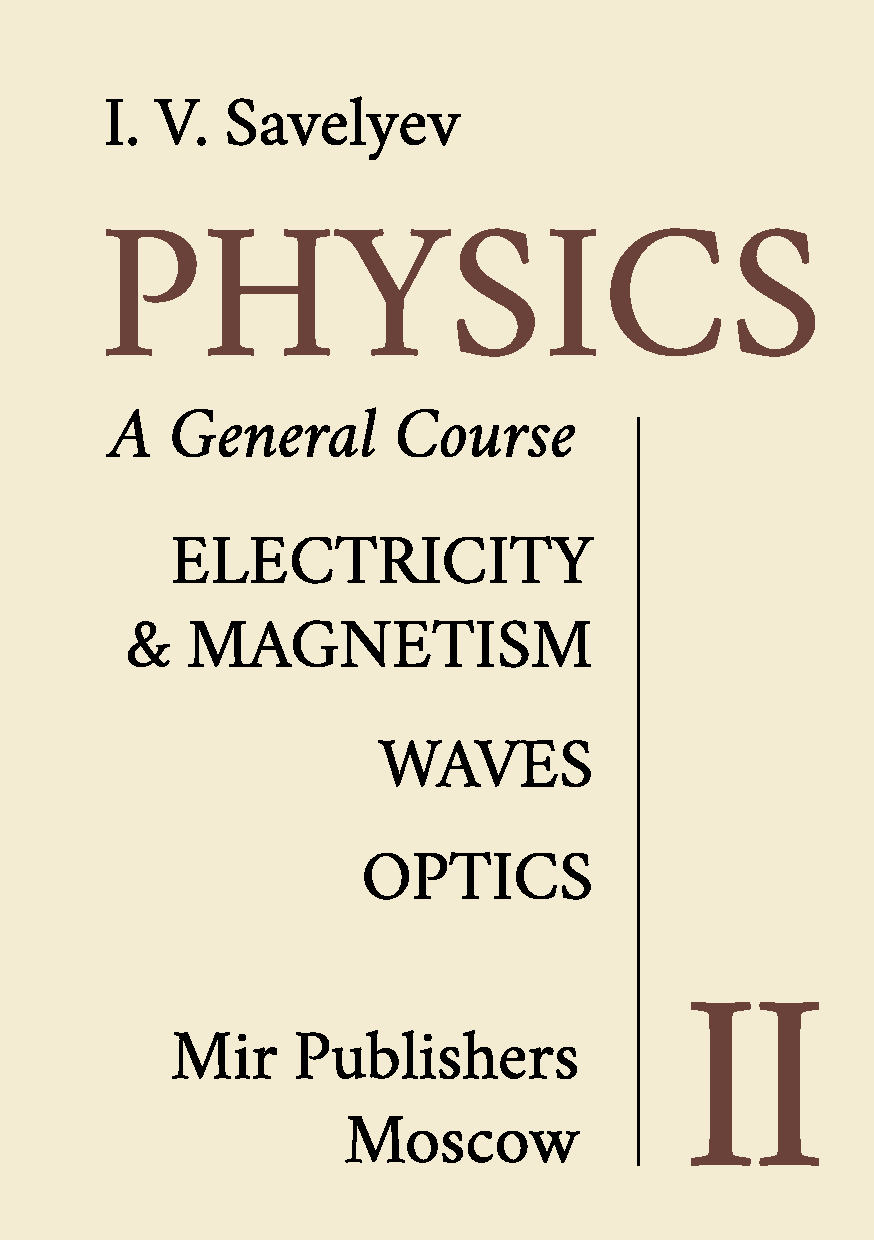
\includepdf{figures/pgc_2_fc.pdf}
\cleardoublepage
% !TEX root = saveliev_physics_general_course_1.tex
%!TEX TS-program = pdflatex
%!TEX encoding = UTF-8 Unicode


%\cleardoublepage
\thispagestyle{empty}
%\maketitle
%\vspace*{1cm}
\noindent
\hspace{50pt}{\large\bfseries I. V. SAVELYEV} \\[40pt]
 
\noindent
\hspace{50pt}{\Huge\bfseries PHYSICS} \\[10pt]

\noindent
\hspace{50pt}{\Large\bfseries A GENERAL COURSE} \\[10pt]

\noindent
\hspace{50pt}{\bfseries (In three volumes)} \\[30pt]

\noindent
\hspace{120pt}{\Large\bfseries VOLUME~I} \\[12pt]

\noindent
\hspace{120pt}{\huge MECHANICS}
\vspace{0.5cm}

\noindent
\hspace{120pt}{\huge MOLECULAR}
\vspace{0.3cm}

\noindent
\hspace{120pt}{\huge PHYSICS}

\vspace*{5cm}
\hspace{120pt}
\includegraphics[width=0.1\textwidth]{figures/mirlogo.pdf}

\hspace{120pt}{\large MIR PUBLISHERS}

\hspace{120pt}{\large MOSCOW}

%\cleardoublepage
\clearpage

\noindent
Translated from Russian by G. Leib

\vspace{40pt}

%Versi\'on electr\'onica publicada en 2020 por\\[1pt]
%Leandro N. Acquaroli
\noindent
First published 1980

\noindent
Revised from the 1977 Russian edition

\noindent
Second printing 1985

\noindent
Third printing 1989

%\url{http://mirtitles.org}

%The project files are available at:

%\url{https://gitlab.com/mirtitles/pfe}

\vfill
\noindent
\textit{Printed in the Union of Soviet Socialist Republics}

\vspace{30pt}

\noindent
ISBN 5-03-000901-9, 1977

\noindent
ISBN 5-03-000900-0, 1980

\thispagestyle{empty}
\cleardoublepage
% !TEX root = saveliev_physics_general_course_1.tex
%!TEX TS-program = pdflatex
%!TEX encoding = UTF-8 Unicode


\chapter*{AUTHOR'S PREFACE TO\\ THE ENGLISH EDITION}
\addcontentsline{toc}{chapter}{Preface}
\chaptermark{\sc Preface}

%\vspace{-1cm}

%\noindent
The present book is the first volume of the three-volume general course in physics. The course is a result of twenty five year's work in the Department of General Physics of the Moscow Institute of Engineering Physics. I was in constant personal contact with my students not only at lectures, but also, perhaps even more importantly, at exercises, consultations, and examinations. These fruitful contacts helped me refine and improve the exposition of the various topics in the course.

The advice and friendly criticism of my colleagues in the department has also been a great help. I would like to make a special mention of the part played by N.~B.~Narozhny, who, in particular, is the author of the original and comparatively simple statistical derivation of the equation $\mathrm{d}S = \mathrm{d}'Q/T$ [\eqn{11_110}].

In writing the book, I have done everything in my power to acquaint students with the basic ideas and methods in physics and to teach them how to think physically. This is why the book is not encyclopedic in its nature. It is mainly devoted to explaining the meaning of physical laws and showing how to apply them consciously. What I have tried to achieve is a deep knowledge of the fundamental principles of physics rather that a shallower acquaintance with the a wide range of questions.

While using the book, try not to memorise the material formalistically and mechanically, but logically, \textit{i.e.}, memorise the material by thoroughly understanding it. I have tried to present physics not as a science for  ``cramming'', not as a certain volume of information to be memorised, but as a clever, logical, and attractive science. It is left to the reader to judge the extent to which I have succeeded in doing this.

Acknowledging the fact that a thick volume by its very appearance makes a student despondent, I have done my utmost to limit the size of the course. This was achieved by carefully choosing the material which in my opinion should be included in a general course of physics. I also tried to be concise, but not at the expense of clarity.

Notwithstanding my desire to reduce the size, I considered it essential to include a number of mathematical sections in the course: on vectors, linear differential equations, the basic concepts of the theory of probability, etc. This was done to impart a ``physical'' tinge to the relevant concepts and relations. In addition, the mathematical ``inclusions'' make it possible to go on with the physics even if, as is often the case, the relevant material has not yet been covered in a mathematics course.

The present course is intended above all for higher technical schools with an extended syllabus in physics. The material has been arranged, however, so that the book can be used as a teaching aid for higher technical schools with ordinary syllabus simply omitting some sections.

\begin{flushright}
	\emph{Igor Savelyev}
\end{flushright}

\noindent
Moscow, July, 1979

%\pagestyle{mystyle}

\cleardoublepage
{\hypersetup{linkcolor=black!80}
	% or \hypersetup{linkcolor=black}, if the colorlinks=true option of hyperref is used
	\tableofcontents
}
\cleardoublepage

\mainmatter

% % !TEX root = saveliev_physics_general_course_2.tex
%!TEX TS-program = pdflatex
%!TEX encoding = UTF-8 Unicode


\chapter*{INTRODUCTION}\label{chap:chapter_introduction}
\addcontentsline{toc}{chapter}{Introduction}
\chaptermark{\sc Introduction}

Physics is a science dealing with the most general properties and forms of motion of matter.

A classical definition of matter was given by V.~Lenin in his book \textit{Materialism and Empirio-Criticism}: ``Matter is a philosophical category denoting the objective reality which is given to man by his sensations, and which is copied, photographed and reflected by our sensations, while existing independently of the''\footnote{V.~I.~Lenin. \textit{Collected Works}, Vol. 14, p. 130. Moscow, Foreign Languages Publishing House (1962).}. Two propositions are significant in this definition, namely, (1) matter is what exists objectively, \ie, independently of anyone's consciousness or sensations, and (2) matter is copied and reflected by our sensations and, consequently, is cognizable.

It follows from the definition of physics that it concentrates knowledge accumulated on the most general properties and phenomena of the world surrounding us. As academician S.~Vavilov noted in one of his articles, ``the extremely common character of a considerable part of the contents of physics, its facts and laws drew physics and philosophy together from time immemorial\ldots. Sometimes physical statements have such a nature that they are difficult to distinguish and separate from philosophical statements, and a physicist must be a philosopher''.

Two kinds of matter are known at present: substance and field. The first kind of matter---substance---includes, for example, atoms, molecules, and all bodies built of them. Electromagnetic, gravitational, and other fields form the second kind of matter. The different kinds of matter can change into each other. For instance, an electron and a positron (representatives of substance) may transform into photons (\ie, into an electromagnetic field). The reverse process is also possible.

Matter is in continuous motion, which is understood to mean any change in general in dialectical materialism\footnote{Dialectical materialism is the name given to the Marxist-Leninist philosophy. The fundamental issue of any philosophy as to what is primary---matter or consciousness---is solved by dialectic materialism in favour of matter when it states that matter is primary and consciousness is secondary. The method of this philosophy is dialectics. It considers matter in constant motion and development whose source is contained in the internal contradictions inherent in objects and phenomena themselves.}. Motion is an inalienable property of matter, which, like matter itself, cannot be created or destroyed. Matter exists and moves in space and in time, which are forms of existence of matter.

The laws of physics are established by generalizing experimental facts. They express the objective regularities existing in nature. These laws are customarily expressed in the form of quantitative relationships between various physical quantities.

The fundamental method of investigation in physics is the running of an experiment, \ie, the observation of the phenomenon being studied in accurately controlled conditions. The latter must permit one to watch the course of the phenomenon and reproduce it each time when these conditions are repeated. Phenomena can be produced experimentally that are not observed in nature. For example, more than ten of the chemical elements known at present have meanwhile not been discovered in nature and were obtained artificially by means of nuclear reactions.

Hypotheses are enlisted to explain experimental data. A hypothesis is a scientific assumption advanced to explain a definite fact or phenomenon and requiring verification and proving to become a scientific theory or law. The correctness of a hypothesis is verified by running the corresponding experiments and by determining whether the corollaries following from the hypothesis agree with the results of experiments and observations. A hypothesis that has successfully passed such verification and has been proved becomes a scientific law or theory.

A physical theory is a system of basic ideas summarizing experimental data and reflecting the objective regularities of nature. A physical theory explains a whole field of natural phenomena from a single viewpoint.

Physics is subdivided into the so-called classical physics and quantum physics. The term classical is applied to the physics whose creation was completed at the beginning of the 20th century. Classical physics was founded by Isaac Newton (1642-1727), who formulated the fundamental laws of classical mechanics. Newtonian mechanics proved to be exceedingly fruitful and mighty, and physicists acquired the conviction that any physical phenomenon can be explained with the aid of Newton's laws.

The edifice of classical physics built up by the end of the last century was very harmonious. Most physicists were convinced that they already knew everything about nature that could be known. The most perspicacious physicists, however, understood that the edifice of classical physics had weak spots. For example, the British physicist William Thomson (Lord Kelvin, 1824-1907) said that there are two dark clouds on the horizon of the cloudless sky of classical physics---the unsuccessful attempts to set up a theory of blackbody radiation, and the contradictory behaviour of ether---the hypothetical medium in which light waves were supposed to propagate. The persistent attempts to surmount these difficulties led to unexpected results. To solve these problems, which were beyond the possibilities of classical physics, it became necessary to revise quite radically the established, habitual notions and introduce concepts that were alien to the spirit of classical physics. Max Planck (1858-1947) succeeded in solving the problem of blackbody radiation in 1900 by introducing the concept of light emission in separate portions---quanta. Thus, at the threshold of the 20th century, the concept of the quantum appeared. It plays an exceedingly important part in modern physics and has resulted in the creation of quantum mechanics.

The contradictory nature of the experimental facts relating to ether induced Albert Einstein (1879-1955) to revise the notions of space and time that were considered to be obvious from Newton's times. The result was the appearance of the theory of relativity. The latter gives equations of motion appreciably differing from those of Newtonian mechanics for bodies travelling with speeds that are noticeable in comparison with the speed of light.

The year 1897 saw the discovery of the electron. The atoms of all the chemical elements were found to contain these particles. Thus, atoms, previously considered indivisible, appeared to have a complicated structure.

The beginning of the 20th century was thus marked in physics by the radical breaking down of numerous habitual concepts and notions. New physical discoveries and theories destroyed the notions of the structure of matter formed by many physicists. Some of them interpreted this as the vanishing of matter. Many physicists lapsed into idealism, and a crisis began in physics.

V.~Lenin in his book \textit{Materialism and Empirio-Criticism} written in 1908 gave annihilating criticism of ``physical'' idealism. He showed that the new discoveries indicate not the vanishing of matter, but the vanishing of the limit up to which matter was known before that time. ``Matter disappears'', wrote Lenin, ``means that the limit within which we have hitherto known matter disappears and that our knowledge is penetrating deeper; properties of matter are likewise disappearing which formerly seemed absolute, immutable, and primary (impenetrability, inertia, mass, etc.) and which are now revealed to be relative and characteristic only of certain states of matter. For the sole 'property' of matter with whose recognition philosophical materialism is bound up is the property of being an objective reality, of existing outside the mind.''\footnote{V.~I.~Lenin. \textit{Collected Works}, Vol. 14, p. 260. Moscow, Foreign Languages Publishing House (1962).}.

The process of recognizing the world is infinite. Our knowledge at any given stage of development of science is due to the historically achieved level of cognition and cannot be considered as final or complete. It is of necessity relative knowledge, \ie, requires further development, further verification, and more precise definition. At the same time, any truly scientific theory, notwithstanding its relativity and incompleteness, contains elements of absolute, \ie, complete, knowledge, and thus signifies a step in the cognition of the objective world. For instance, mechanics based on Newton's laws is not correct, strictly speaking. But for a certain range of phenomena, this mechanics is quite satisfactory. Thus, the development of science did not cross out Newtonian mechanics. It only established the limits within which it is correct. Newtonian mechanics formed a constituent part of the general edifice of the physical science.

The beginning of the 20th century is characterized by persistent attempts to penetrate into the internal structure of atoms. The key to determining their structure was found to be the studying of atomic spectra. The theory of the atom developed by Niels Bohr (1885-1962) in 1913 was the first striking success in explaining the observed spectra. This theory, however, has obvious features of inconsistency: in addition to the motion of an electron in an atom obeying the laws of classical mechanics, the theory imposes special quantum restrictions on this motion. The theory soon had to pay for this lack of consistency. After the first successes in explaining the spectra of the simplest atom---that of hydrogen---it was found that Bohr's theory is unable to explain the behaviour of atoms with two or more electrons.

The need to develop a new comprehensive theory of atoms became pressing. A bold hypothesis of Louis de Broglie put forward in 1924 placed the cornerstone in such a theory. It was known by that time that light, while being a wave process, also exhibits a corpuscular nature in a number of cases, \ie, behaves like a stream of particles. De Broglie put forth the idea that the particles of a substance, in turn, should display wave properties too in definite conditions. De Broglie's hypothesis soon received a brilliant experimental confirmation---it was proved that a wave process is associated with the particles of a substance, and it must be taken into account when considering the mechanics of an atom. A result of this discovery was the development by Erwin Schr\"odinger (1887-1961) and Werner Heisenberg (1901-1976) of a new physical theory---wave or quantum mechanics. The latter achieved striking successes in explaining atomic processes and the structure of a substance. Results were obtained that showed excellent agreement with experimental data when 'it was found possible to surmount the mathematical difficulties.

The latest decades were noted by remarkable achievements in the field of studying the atomic nucleus. Scientists and engineers have mastered nuclear processes to such an extent that the practical use of nuclear energy has become possible. One of the leading places in this field belongs to Soviet physics. Particularly, the first atomic power plant in the world was erected in the USSR.

Finally, in recent years, the walls of laboratories created by the hands of man were moved apart beyond the limits of our globe. On October 4, 1957, an artificial satellite of the Earth was launched in the Soviet Union the first time in history. It was a small laboratory outfitted with apparatus for scientific research. April 12, 1961, saw the first flight of a man into outer space. The first Soviet cosmonaut, Yuri Gagarin, flew around the Earth and landed safely. The first space rockets were built in the Soviet Union. They left the field of the Earth's attraction and transmitted to the Earth by means of radio signals valuable results of studying outer space and, particularly, photographs of the reverse side of the Moon. In 1969, U.S. astronauts landed on the Moon. In 1975, two Soviet automatic spaceships made a soft landing on Venus and transmitted valuable information on the physical conditions on this planet, and also photographs of its surface.

There is no doubt that the nearest future will be marked with new fundamental discoveries in the science of physics.

%\pagestyle{mystyle}

% \cleardoublepage

\part{ELECTRICITY AND MAGNETISM}\label{part:A}
\cleardoublepage
%% !TEX root = saveliev_physics_general_course_2.tex
%!TEX TS-program = pdflatex
%!TEX encoding = UTF-8 Unicode


\chapter{ĐIỆN TRƯỜNG TRONG CHÂN KHÔNG}\label{chap:1}

\section{Điện Tích}\label{sec:1_1}

Tất cả các vật thể trong tự nhiên đều có thể bị nhiễm điện, hay nhận điện tích. Khi vật thể bị nhiễm điện, nó sẽ tương tác với một vật thể nhiễm điện khác. Có hai loại điện tích tồn tại. Nó thường được gọi là điện tích dương và âm. Những điện tích cùng dấu thì hút nhau, trái dấu thì đẩy nhau.

Điện tích là một phần tử được cấu thành từ các hạt nguyên tố\footnote{Hạt nguyên tố được định nghĩa là những hạt vi mô mà với trình độ vật lý hiện tại, nội cấu trúc của nó không được coi như được cấu tạo từ những hạt khác.}. Điện tích của tất cả các hạt nguyên tố (trừ khi nó không tồn tại) có độ lớn như nhau. Nó được gọi là \textbf{điện tích nguyên tố}. Chúng ta sẽ sử dụng biểu tượng $e$ để ký hiệu cho điện tích nguyên tố dương. 

Những hạt nguyên tố bao gồm electron (mang điện tích âm), proton (mang điện tích dương), và neutron (không mang điện tích). Những hạt này là nền tảng để tạo nên nguyên tử, phân tử của tất cả vật thể, và vì thế tất cả vật thể đều có điện tích. Trong các vật thể, những hạt có dấu trái nhau có số lượng bằng nhau và phân bố với mật độ như nhau. Tổng đại số của tất cả các điện tích trong trường hợp này thì bằng không, và mỗi thể tích nguyên tố (cũng như là trên toàn bộ vật thể) sẽ trung hoà về điện tích. Nếu bằng một cách nào đó chúng ta tăng thêm số lượng hạt cùng dấu trong vật thể (cũng như là giảm bớt số lượng hạt ngược dấu), thì vật thể sẽ bị tích điện. Hơn nữa, hoàn toàn khả thi để tích điện mà không cần thay đổi tổng số lượng hạt âm và dương, chỉ cần phân bố lại điện tích trong vật thể. Việc này khiến cho một phần của vật thể có thừa điện tích của một dấu và phần khác bị thừa điện tích ngược dấu. Điều này có thể được thực hiện bằng việc đưa một vật thể tích điện đến gần kim loại chưa tích điện.

Vì điện tích $q$ được tạo nên bởi một số nguyên các $e$, nên
\begin{equation}\label{eq:1_1}
	q = \pm N e.
\end{equation}

\noindent
Một điện tích cơ bản rất nhỏ, đến nỗi các vật mang điện tích vĩ mô có thể được coi là mang điện tích phân bố liên tục.

Nếu một đại lượng vật lý chỉ có thể nhận các giá trị rời rạc, thì nó được gọi là bị lượng tử hoá. Điều này đã được chỉ ra trong \eqn{1_1}, rằng điện tích bị lượng tử hoá. 

Độ lớn của một điện tích là như nhau trong mọi hệ quy chiếu quán tính. Vì thế, điện tích được cho là có tính chất bất biến tương đối tính. Điều này dẫn đến việc độ lớn của điện tích không phụ thuộc vào trạng thái của điện tích là đứng yên hay di chuyển.

Điện tích có thể biến mất và xuất hiện lại. Hai điện tích cơ bản khác dấu tồn tại và biến mất tại cùng một thời điểm. Ví dụ, một electron và một positron (positron là electron mang điện tích dương) khi tiếp xúc với nhau sẽ xảy ra hiện tượng sự hủy hạt, khi đó chúng biến thành một gamma-photon trung hoà về điện. Điều này xảy ra là bởi sự biến mất của $-e$ và $+e$. Ngược lại, trong quá trình sinh cặp, một gamma-photon đi vào trường của một hạt nhân nguyên tử, và biến thành một cặp hạt---một electron và một positron. Quá trình này sinh ra điện tích $-e$và $+e$.

Như vậy, tổng điện tích của hệ mang điện cô lập\footnote{Một hệ mang điện được coi là cô lập nếu như không một bất cứ điện tích nào có thể thoát khỏi hoặc thêm vào hệ thông qua biên giới của hệ} là không đổi. Đây chính là phát biểu của \textbf{định luật bảo toàn điện tích}.

Chúng ta cần lưu ý rằng, định luật bảo toàn điện tích liên hệ mật thiết với sự bất biến tương đối tính của điện tích. Vì nếu độ lớn của điện tích phụ thuộc vào vận tốc của nó, vậy thì khi ta dời một điện tích của một dấu, chúng ta sẽ kiến tổng điện tích của hệ cô lập bị thay đổi.

\section{Định luật Coulomb}\label{sec:1_2}

Định luật được tuân theo bởi lực tương tác của các điện tích điểm được thực nghiệm thành lập vào năm 1785 bởi nhà vật lý người Pháp Charles A. de Coulomb (1736-1806). Một \textbf{điện tích điểm} được định nghĩa là một vật mang điện mà kích thước của nó có thể bỏ qua khi so với khoảng cách từ nó tới những vật thể mang điện khác.

Sử dụng một cái cân xoắn (\fig{1_1}) tương tự với cái được sử dụng bởi H. Cavendish để xác định hằng số hấp dẫn (xem Vol. I, Sec. 6.1), Coulomb đo được lực tương tác của hai quả cầu mang điện phụ thuộc vào độ lớn điện tích của chúng và khoảng cách giữa chúng. Ông ấy bắt đầu từ thực tế rằng khi một quả cầu kim loại mang điện tiếp xúc với một quả cầu giống hệt nhưng không mang điện, điện tích sẽ được phân bố như nhau giữa hai quả cầu.

\begin{figure}[!htb]
	\begin{center}
		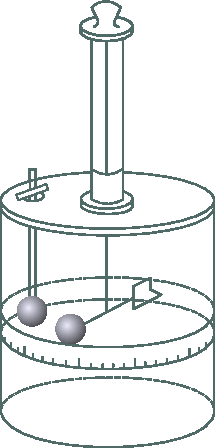
\includegraphics[scale=0.9]{figures/ch_01/fig_1_1.pdf}
		\caption[]{}
		\label{fig:1_1}
	\end{center}
	\vspace{-0.8cm}
\end{figure}

Như là kết quả từ thực nghiệm, Coulomb dẫn đến kết luận rằng \textit{lực tương tác giữa hai điện tích điểm đứng yên tỷ lệ thuận với độ lớn điện tích của mỗi hạt và tỷ lệ nghịch với bình phương khoảng cách giữa chúng}. Hướng của lực trùng với đường thẳng nối các điện tích.

Cần lưu ý rằng hướng của lực tương tác dọc theo đường thẳng nối các điện tích điểm đến từ việc xem xét tính đối xứng. Một không gian trống được giả định là đồng tính và đẳng hướng. Kết quả là, hướng duy nhất khác biệt trong không gian chứa các điện tích tĩnh là từ một điện tích tới các điện tích khác. Giả sử rằng lực $\vec{F}$ tác dụng lên điện tích $q_i$ (\fig{1_2}) tạo một góc $\alpha$ với hướng từ $q_1$ tới $q_2$, và $\alpha$ khác $0$ hoặc $\pi$. Nhưng do tính đối xứng trục, không có căn cứ để xác định lực  $\vec{F}$ khỏi vô số các lực có hướng khác nhưng đều tạo góc  $\alpha$ với trục $q_1$-$q_2$ (hướng của các lực này tạo thành một hình nón với góc ở đỉnh $2\alpha$). Khó khăn xuất hiện như kết quả của điều này biến mất khi $\alpha$ bằng $0$ hoặc $\pi$.

\begin{figure}[!htb]
	\begin{minipage}[t]{0.5\linewidth}
		\begin{center}
			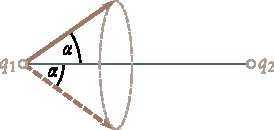
\includegraphics[scale=1]{figures/ch_01/fig_1_2.pdf}
			\caption[]{}
			\label{fig:1_2}
		\end{center}
	\end{minipage}
	\hspace{-0.05cm}
	\begin{minipage}[t]{0.5\linewidth}
		\begin{center}
			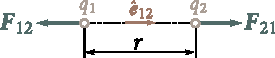
\includegraphics[scale=1]{figures/ch_01/fig_1_3.pdf}
			\caption[]{}
			\label{fig:1_3}
		\end{center}
	\end{minipage}
\vspace{-0.4cm}
\end{figure}

Định luật Coulomb có thể được biểu diễn thông qua biểu thức
\begin{equation}\label{eq:1_2}
	\vec{F}_{12} = -k \frac{q_1 q_2}{r^2}\,\vecuni{12}.
\end{equation}

\noindent
Ở đây, $k$ là một hằng số tỷ lệ được cho là dương, $q_1$ và $q_2$ là độ lớn của những điện tích tương tác, $r$ là khoảng cách giữa các điện tích, $\vecuni{12}$ là vector đơn vị hướng từ điện tích $q_1$ tới $q_2$ và $\vec{F}_{12}$ là lực tác dụng lên điện tích $q_1$ (\fig{1_3}; hình ảnh tương ứng cho trường hợp này).

Lực $\vec{F}_{21}$ khác $\vec{F}_{12}$ ở dấu của nó:
\begin{equation}\label{eq:1_3}
	\vec{F}_{21} = k \frac{q_1 q_2}{r^2}\,\vecuni{12}.
\end{equation}

Độ lớn của lực tương tác, là như nhau cho cả hai điện tích, có thể được viết ở dạng
\begin{equation}\label{eq:1_4}
	F = k \frac{\absolute{q_1 q_2}}{r^2}.
\end{equation}

Thí nghiệm chỉ ra rằng lực tương tác giữa hai điện tích đã cho không đổi khi có các điện tích khác đặt gần chúng. Giả sử chúng ta có điện tích $\ab{q}{a}$ và, thêm vào đó, $N$ điện tích khác $q_1, q_2,\ldots, q_N$. Từ trên có thể thấy rằng lực tổng hợp $\vec{F}$ từ $N$ điện tích $q_i$ tác dụng lên $\ab{q}{a}$ là
\begin{equation}\label{eq:1_5}
	\vec{F} = \sum_{i=1}^N \ab{\vec{F}}{a, $i$}
\end{equation}

\noindent
Với $\ab{\vec{F}}{a, $i$}$ là lực mà điện tích $q_i$ tác dụng lên $\ab{q}{a}$ trong sự có mặt của $N-1$ điện tích khác.

Thực tế thể hiện bởi \eqn{1_5} cho phép chúng ta tính toán lực tương tác giữa những điện tích tập trung trên các vật thể có kích thước hữu hạn, nhờ định luật của sự tương tác giữa các điện tích điểm. Với mục đích này, chúng ta phải chia mỗi vật mang điện thành những điện tích nhỏ $\deriv{q}$ có thể coi như chất điểm, sử dụng \eqn{1_2} để tính lực tương tác giữa các cặp điện tích $\deriv{q}$, sau đó thực hiện tổng hợp vector từ những lực này. Về mặt toán học, phương pháp này hoàn toàn giống với việc tính toán lực hấp dẫn giữa các vật thể có kích thước hữu hạn (xem Vol. I, Sec. 6.1).

Tất cả dữ kiện thực nghiệm có sẵn dẫn đến kết luận rằng định luật Coulomb sử dụng được cho khoảng cách từ \SI{e-15}{\metre} tới ít nhất vài kilomet. Có cơ sở để cho rằng định luật không còn đúng nữa đối với khoảng cách nhỏ hơn \SI{e-16}{\metre}. Với khoảng cách rất lớn, Không có sự xác nhận thực nghiệm cho định luật Coulomb. Nhưng cũng không có lý do để cho rằng định luật này không còn được tuân thủ với khoảng cách rất lớn giữa các điện tích.

\section{Hệ Thống Đơn Vị}\label{sec:1_3}

Chúng ta có thể tạo một hằng số tỉ lệ trong phương trình \eqn{1_2} bằng cách chọn đơn vị cho điện tích (đơn vị của $F$ và $r$ đã được thành lập trong cơ học). Đơn vị của điện tích (khi $F$ và $r$ được đo trong hệ đơn vị cgs) được gọi là \textbf{đơn vị tĩnh điện tuyệt đối} của điện tích (cgse$_q$). Nó là độ lớn của hai điện tích giống nhau tương tác với nhau qua một lực \SI{1}{\dyne} và cách nhau chúng cách nhau \SI{1}{\centi\metre}

Đo lường chi tiết (được mô tả ở \sect{10_3}) cho ta biết giá trị điện tích cơ bản là
\begin{equation}\label{eq:1_6}
	e = \num{4.80e-10}\text{cgse$_q$}.
\end{equation}

Giống như các đơn vị cơ bản như độ dài, khối lượng, thời gian, thì điện tích cũng là một đơn vị cơ bản mà chúng ta dùng để xây dựng hệ thống đơn vị của điện từ học. Hệ thống dựa trên các đơn vị như centimet, gram, giây, và cgse$_q$ còn được gọi là \textbf{hệ thống đơn vị tĩnh điện tuyệt đối} (hệ thống cgse). Nó được tìm ra bởi định luật Coulomb, hay định luật tương tác giữa các điện tích nghỉ. Trong những phần sau, chúng ta sẽ trở nên quen thuộc với \textbf{hệ thống đơn vị điện từ tuyệt đối} (hệ thống cgsm), hệ thống này dựa trên các định luật tương tác giữa các vật dẫn mang dòng điện. Hệ Gauss cũng sử dụng các đơn vị giống với cả hệ thống cgse và cgsm, và nó cũng là một hệ thống đơn vị tuyệt đối.

Phương trình \eqref{eq:1_4} trong hệ cgse sẽ trở thành
\begin{equation}\label{eq:1_7}
	F = \frac{\absolute{q_1 q_2}}{r^2}.
\end{equation}

\noindent
Phương trình chỉ đúng đối với môi trường đang xét là chân không. Nó cần phải xem xét kĩ hơn nếu xét trong môi trường là điện môi.

USSR State Standard GOST 9867-61 có hiệu lực vào ngày 1, tháng 1, 1963, đề xuất về việc sử dụng Hệ Thống Đơn Vị Quốc Tế (SI). Những đơn vị cơ bản trong hệ thống này là mét, kilogram, giây, ampere, kelvin, candela, và mole. Đơn vị của lực trong hệ SI là (\si{\newton}) bằng với \num{e5} dynes. 

Để thành lập các đơn vị trong hệ SI cho các đại lượng điện từ học, ta có thể suy ra từ các định luật. Giống như trong hệ cgsm, các đơn vị được suy ra từ định luật tương tác giữa các vật mang dòng điện. Điều đó dẫn đến việc, hằng số tỉ lệ trong phương trình Coulomb sẽ là đại lượng có thứ nguyên và riêng biệt so với các đơn vị khác.

Đơn vị SI của điện tích là Coulomb (\si{\coulomb}. Nó đã được tìm ra bởi các đo đạc thực nghiệm
\begin{equation}\label{eq:1_8}
	\SI{1}{\coulomb} = \num{2.998e9} \approx \num{3e9}{\text{ cgse$_q$}}.
\end{equation}

Để tìm giá trị của một đơn vị điện tích, ta sẽ đi tính toán lực tương tác giữa hai điện tích có giá trị \SI{1}{\coulomb} và chúng cách nhau \SI{1}{\metre}.
\begin{equation}\label{eq:1_9}
	F = \frac{\num{3e9}\times\num{3e9}}{100^2}\,\text{ cgse$_F$} = \SI{9e14}{\dyne} = \SI{9e9}{\newton} \approx \SI{e9}{\kgf}.
\end{equation}

Một điện tích cơ bản có thể được biểu diễn trong coulombs là
\begin{equation}\label{eq:1_10}
	e = \SI{1.60e-19}{\coulomb}.
\end{equation}

\section{Hiệu Chỉnh Các Công Thức}\label{sec:1_4}

Có nhiều công thức trong điện từ học khi được viết trong hệ cgs (đặc biệt trong hệ Gauss) có thành phần $4\pi$ và hằng số tốc độ ánh sáng trong chân không $c$. Để loại bỏ những thành phần này ra khỏi công thức, mà quan trọng trong thực tiễn, ta cho hằng số tỉ lệ trong định luật Coulomb bằng $1/4\pi\varepsilon_0$. Phương trình của điện tích trong chân không trở thành
\begin{equation}\label{eq:1_11}
	F = \frac{1}{4\pi\varepsilon_0}\frac{\absolute{q_1 q_2}}{r^2}.
\end{equation}

\noindent
Những công thức khác cũng thay theo đó. Việc thay đổi cách viết công thức được gọi là \textbf{hiệu chỉnh}. Hệ thống đơn vị được cấu tạo từ những công thức được hiệu chỉnh cũng được gọi là \text{hiệu chỉnh}.

Đại lượng $\varepsilon_0$ được gọi là \textbf{hằng số điện}. Nó có thứ nguyên là điện dung trên độ dài. Nó còn được biểu diễn dưới đơn vị farad trên mét. Để tìm được giá trị của $\varepsilon_0$, chúng ta sẽ tìm giá trị của lực tương tác trong \eqn{1_11} giữa hai điện tích có giá trị \SI{1}{\coulomb}, và chúng cách nhau \SI{1}{\metre}. Theo \eqn{1_9}, lực tương tác trong trường hợp này là \SI{9e9}{\newton}. Sử dụng giá trị này của lực, cũng như $q_1=q_2=\SI{1}{\coulomb}$ và $r=\SI{1}{\metre}$ vào phương trình \eqn{1_11}, chúng ta sẽ có được
\begin{equation*}
	\num{9e9} = \frac{1}{4\pi\varepsilon_0}\frac{\absolute{1\times 1}}{1^2}
\end{equation*}

\noindent
Hay
\begin{equation}\label{eq:1_12}
	\varepsilon_0 = \frac{1}{4\pi\times\num{9e9}} = \SI{0.885e-11}{\faraday\per\metre}.
\end{equation}

Hệ thống đơn vị Gauss được sử dụng rộng rãi, và tiếp tục được sử dụng trong công đồng vật lý. Vì thế, chúng ta xem trọng việc giúp các độc giả làm quen với cả hệ SI và hệ Gauss. Chúng ta nên trình bày các đại lượng trong đơn vị SI và Gauss cùng một lúc trong cùng một công thức. Các công thức quan trọng trong điện từ học trong cả hệ SI và Gauss được so sánh trong \app{A_3}

\section{Điện Trường.Cường Độ Điện Trường}\label{sec:1_5}

Một điện tích nghỉ tương tác thông qua một trường điện\footnote{Chúng ta sẽ thấy trong \sect{6_2}, nếu một điện tích đang di chuyển, nó còn tạo ra từ trường.}. Một điện tích làm thay đổi tính chất của môi trường xung quanh nó---nó sẽ tạo ra một trường điện. Nếu đặt một điện tích trong trường, nó sẽ chịu một lực. Vì thế, để tìm xem có điện trường không, ta chỉ cần đặt một vật thể nhiễm điện (từ giờ, chúng ta sẽ gọi ngắn gọn là điện tích) trong trường và xem xét lực tác dụng lên điện tích đó.

Do đó, để tìm hiểu và nghiên cứu về điện trường, chúng ta sẽ sử dụng đến điện tích ``thử''. Để lực tác dụng lên điện tích thử tại ``một điểm cho trước'' được xác định, thì điện tích thử buộc phải là chất điểm. Nếu không, lực tác dụng lên điện tích thử sẽ là tổng hợp các lực tác dụng lên từng phần thể tích nhỏ của nó. 

\begin{figure}[!htb]
	\begin{center}
		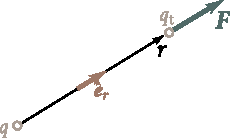
\includegraphics[scale=1]{figures/ch_01/fig_1_4.pdf}
		\caption[]{}
		\label{fig:1_4}
	\end{center}
	\vspace{-0.8cm}
\end{figure}

Chúng ta sẽ đi tìm hiểu về điện trường gây ra bởi một điện tích cố định $q$, bằng các sử dụng điện tích thử để xác định nó. Chúng ta đặt điện tích thử vào trường, sao cho $\vec{r}$ là vector xác định vị trí của nó đối với điện tích $q$ (\fig{1_4}). Chúng ta thấy rằng, điện tích thử sẽ chịu một lực
\begin{equation}\label{eq:1_13}
	\vec{F} = \ab{q}{t} \parenthesis{
	\frac{1}{4\pi\varepsilon_0} \frac{q}{r^2}\,\vecuni{r}
	}
\end{equation}

\noindent
[xem phương trình \eqref{eq:1_3} và \eqref{eq:1_11}]. Ở đây, $\vecuni{r}$ là vector đơn vị của vector vị trí $\vec{r}$.

Khi nhìn vào \eqn{1_13} chúng ta thấy rằng, lực tác dụng lên điện tích thử không chỉ phụ thuộc vào các đại lượng đặc trưng của trường (là $q$ và $\vec{r}$), nhưng còn phụ thuộc vào độ lớn của điện tích thử $\ab{q}{t}$. Nếu chúng ta xét các điện tích thử $\ab{q}{t}'$,$\ab{q}{t}''$, \ldots, thì lực $\vec{F'}$,$\vec{F''}$, \ldots tương ứng sẽ khác nhau.
Chúng ta có thể thấy từ \eqn{1_13}, rằng tỉ lệ $F/\ab{q}{t}$ cho bất kì một điện tích thử nào đều như nhau, và tỉ lệ này chỉ phụ thuộc vào đại lượng  $q$ và $\vec{r}$. Vì thế, nó sẽ trở nên tự nhiên hơn nếu chúng ta sử dụng tỉ lệ này đại lượng để xác định điện trường:
\begin{equation}\label{eq:1_14}
	\vec{E} = \frac{\vec{F}}{\ab{q}{t}}.
\end{equation}

\noindent
Đại lượng vector này được gọi là \textbf{cường độ điện trường} (hay \textbf{độ mạnh điện trường}) tại một điểm xác định (hay tại một điểm mà điện tích thử $\ab{q}{t}$ chịu một lực $\vec{F}$).

Theo \eqn{1_14}, cường độ điện trường bằng với lực tác dụng lên một đơn vị điện tích, tại một vị trí xác định. Hướng của vector $\vec{E}$ sẽ trùng với hướng của lực nếu điện tích thử dương, còn nếu điện tích thử là âm thì ngược lại.

Cần lưu ý rằng \eqn{1_14} vẫn đúng cho trường hợp điện tích thử âm ($\ab{q}{t}<0$). Trong trường này, vector $\vec{E}$ và vector $\vec{F}$ ngược hướng.

Chúng ta đã tiếp cận với ý tưởng về cường độ điện trường khi nghiên cứu về một điện tích điểm cố định. Nhưng định nghĩa về $\vec{E}$ trong \eqref{eq:1_14} cũng đúng cho trường hợp hệ gồm nhiều điện tích. Tuy nhiên, chúng ta cần phải lưu ý vài chỗ. Các điện tích trong một hệ sẽ bị phân bố lại dưới sự tác dụng của điện tích thử. Điều này là hoàn toàn có thể xảy ra, ví dụ, điện tích của hệ nằm trong một vật dẫn. Mặt khác các điện tích này có thể chuyển động tự do trong vật dẫn. Để tránh sự phân bố lại điện tích trong hệ, ta sẽ sử dụng một điện tích thử có giá trị vô cùng bé.

Theo \eqref{eq:1_13} và \eqref{eq:1_14}, cường độ điện trường tạo ra bởi một điện tích điểm tỉ lệ thuận với độ lớn của $q$ và tỉ lệ nghịch với bình phương khoảng cách $r$ từ điện tích đến điểm đang xét:
\begin{equation}\label{eq:1_15}
	\vec{E} = \frac{1}{4\pi\varepsilon_0} \frac{q}{r^2}\, \vecuni{r}.
\end{equation}

\noindent
Vector $\vec{E}$ nằm dọc trên đường thẳng chứa điện tích và điểm đang xét trong trường. Nó có hướng từ điện tích đi ra xa nếu điện tích dương, và có hướng từ xa vô cùng đến điện tích nếu điện tích âm.

Trong hệ Gauss, phương trình cho cường độ điện trường của một điện tích điểm trong chân không có dạng là:
\begin{equation}\label{eq:1_16}
	\vec{E} = \frac{q}{r^2}\, \vecuni{r}.
\end{equation}

Đơn vị của cường độ điện trường là cường độ tại một điểm mà có một đơn vị lực (\SI{1}{\newton} trong hệ SI và \SI{1}{\dyne} trong hệ Gauss) tác dụng lên một đơn vị điện tích (\SI{1}{\coulomb} trong hệ SI và \num{1}\cgse{q} trong hệ Gauss). Đơn vị của cường độ điện trường không có tên riêng trong hệ Gauss. Trong hệ SI thì nó có đơn vị là volt trên mét (\si{\volt\per\metre}) [xem \eqn{1_44}].

Theo \eqn{1_15}, một điện tích \SI{1}{\coulomb} sẽ tạo ra một cường độ điện trường trong chân không tại một điểm cách nó một khoảng \SI{1}{\metre} là:
\begin{equation*}
	E = \frac{1}{4\pi\parenthesis{1/4\pi \times \num{9e9}}} \frac{1}{1^2} = \SI{9e9}{\volt\per\metre}.
\end{equation*}

Xét trong hệ Gauss ta có
\begin{equation*}
	E = \frac{q}{r^2} = \frac{\num{3e9}}{100^2} = \num{3e5}\cgse{E}.
\end{equation*}

\noindent
So sánh hai đáp án trên ta có:
\begin{equation}\label{eq:1_17}
	1\cgse{E} = \SI{3e4}{\volt\per\metre}.
\end{equation}

Theo \eqn{1_14}, lực tác dụng lên điện tích thử là
\begin{equation*}
	\vec{F} = \ab{q}{t} \vec{E}.
\end{equation*}

\noindent
Dễ dàng thấy rằng, bất kì điện tích điểm $q$\footnote{Trong \eqn{1_15}, $q$ là điện tích thiết lập nên trường. Trong \eqn{1_18}, $q$ là điện tích chịu tác dụng của lực $\vec{F}$ tại điểm có cường độ $\vec{E}$.} nào được đặt tại điểm có cường độ điện trường $\vec{E}$, sẽ chịu một lực
\begin{equation}\label{eq:1_18}
	\vec{F} = q \vec{E}.
\end{equation}

\noindent
Nếu điện tích $q$ dương, thì hướng của lực sẽ trùng với hướng của vector $\vec{E}$. Ngược lại, nếu $q$ âm, thì vector $\vec{F}$ sẽ ngược chiều $\vec{E}$.

Chúng ta đã đề cập đến ở \sect{1_2}, rằng lực gây ra bởi một hệ các điện tích sẽ bằng tổng hợp vector lực của từng thành phần trong hệ [xem \eqn{1_15}]. Do đó, nó sẽ đúng khi phát biểu \textit{điện trường gây ra bởi hệ các điện tích, tại một điểm nào đó, sẽ bằng tổng hợp vector điện trường của từng thành phần trong hệ}:
\begin{equation}\label{eq:1_19}
	\vec{E} = \sum_i \vec{E}_i.
\end{equation}

\noindent
Nhận định này được gọi là \textbf{nguyên lý chồng chất điện trường}

Nguyên lý chồng chất cho phép chúng ta tính toán điện trường của một hệ điện tích bất kì. Bằng cách chia nhỏ vật thể nhiễm điện thành những thành phần $\deriv{q}$ rất nhỏ, chúng ta sẽ biến hệ điện tích thành một tập hợp các điện tích điểm. Sau đó, chúng ta chỉ cần tính toán tác dụng của từng điện tích đó lên điểm đang xét theo \eqn{1_15}

Điện trường có thể mô tả qua việc xác định độ lớn và hướng của vector $\vec{E}$ tại một điểm. Tổng hợp những vector này lại sẽ tạo nên một trường vecor cường độ điện trường (so sánh với trường vector vận tốc, Vol. I, Sec. 9.1). Trường vector vận tốc được mô tả bằng các đường dòng. Tương tự, đối với điện trường, chúng ta cũng có thể mô tả nó dưới dạng các đường dòng, mà chúng ta có thể gọi ngắn gọn là đường sức điện. Mật độ đường sức bằng với số đường sức đi qua một đơn vị diện tích (vuông góc với $\vec{E}$), và nó có giá trị bằng với độ lớn của vector $\vec{E}$. Do đó, hình dạng của đường sức cho phép chúng ta xác định được độ lớn và hướng của $\vec{E}$ tại một điểm bất kì (\fig{1_5}).

\begin{figure}[!htb]
	\begin{minipage}[t]{0.5\linewidth}
		\begin{center}
			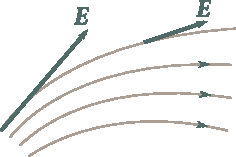
\includegraphics[scale=1]{figures/ch_01/fig_1_5.pdf}
			\caption[]{}
			\label{fig:1_5}
		\end{center}
	\end{minipage}
	\hspace{-0.05cm}
	\begin{minipage}[t]{0.5\linewidth}
		\begin{center}
			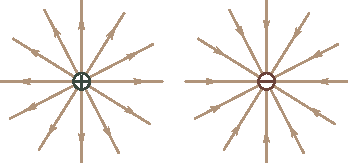
\includegraphics[scale=1]{figures/ch_01/fig_1_6.pdf}
			\caption[]{}
			\label{fig:1_6}
		\end{center}
	\end{minipage}
\vspace{-0.4cm}
\end{figure}

Đường sức của một điện tích điểm là các đường thẳng xuyên tâm, có hướng đi ra xa khỏi điện tích (nếu nó dương), hoặc hướng vào điện tích (nếu nó âm). Điện tích là một đầu mút của đường sức, đầu mút còn lại thì ở xa vô cùng. Chúng ta có, tổng đường sức xuyên qua một mặt cầu có bán kính $r$ sẽ bằng với tích của mật độ đường sức với diện tích bề mặt của mặt cầu $4\pi r^2$. Cho rằng mật độ đường sức có giá trị đại số là $E=(1/4\pi\varepsilon_0)(q/r^2)$. Vì thế, ta có số đường sức xuyên qua toàn bộ mặt cầu là $(1/4\pi\varepsilon_0)(q/r^2) 4\pi r^2=q/\varepsilon_0$. Kết quả này cho ta thấy rằng tổng số đường sức điện xuyên qua một mặt bao quanh điện tích là như nhau. Chúng ta cũng có thể suy ra rằng, các đường sức luôn có một đầu mút là điện tích, và đường sức sẽ hướng từ điện tích ra xa (nếu điện tích dương) hoặc hướng từ vô cùng về điện tích (nếu điện tích âm). Tính chất này của đường sức điện là cơ bản trong trường tĩnh điện, hay đường sức của một hệ điện tích cố định chỉ có thể bắt đầu, và kết thúc duy nhất tại ngay điện tích.

\section{Điện Thế}\label{sec:1_6}

Chúng ta cùng xem xét trường điện trường gây ra bởi một điện tích điểm cố định $q$. Tại một điểm bất kì trong trường, điện tích $q'$ sẽ chịu một lực
\begin{equation}\label{eq:1_20}
	\vec{F} = \frac{1}{4\pi\varepsilon_0}\frac{qq'}{r^2}\, \vecuni{r} = F(r)\vecuni{r}.
\end{equation}

\noindent
Ở đây $F(r)$ là độ lớn của lực $\vec{F}$, $\vec{r}$ là vector giúp xác định vị trí của $q'$ so với $q$, có vector đơn vị là $\vecuni{r}$.

\begin{figure}[!htb]
	\begin{center}
		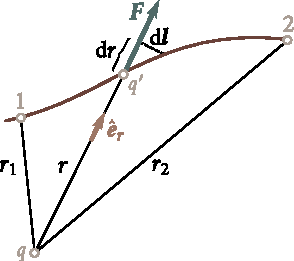
\includegraphics[scale=1]{figures/ch_01/fig_1_7.pdf}
		\caption[]{}
		\label{fig:1_7}
	\end{center}
	\vspace{-0.8cm}
\end{figure}

Lực trong \eqref{eq:1_20} là một lực xuyên tâm (xem Vol. I, Sec. 3.4). Trường xuyên tâm có tính bảo toàn. Vì thế, công của điện trường tác dụng lên điện tích $q'$ khi di chuyển từ một điểm đến một vị trí khác là không phụ thuộc vào hình dạng đường đi. Công này được tính là:
\begin{equation}\label{eq:1_21}
	A_{12} = \int_1^2 F(r) \vecuni{r}\, \deriv{\vec{l}}
\end{equation}

\noindent
Trong đó $\deriv{\vec{l}}$ là độ dời nguyên tố của điện tích $q'$. Hình \fig{1_7} cho chúng ta thấy rằng tích vô hướng của $\vecuni{r}\,\deriv{\vec{l}}$ bằng với biến thiên độ lớn của vector $\vec{r}$, hay $\deriv{r}$. Phương trình \eqref{eq:1_21} có thể được viết dưới dạng
\begin{equation*}
	A_{12} = \int_1^2 F(r)\, \deriv{r}
\end{equation*}

\noindent
[so sánh với phương trình (3.24) của Vol. I]. Sử dụng biểu thức của $F(r)$ ta sẽ có:
\begin{equation}\label{eq:1_22}
	A_{12} = \frac{qq'}{4\pi\varepsilon_0} \int_{r_1}^{r_2} \frac{\deriv{r}}{r^2} = \frac{1}{4\pi\varepsilon_0} \parenthesis{
	\frac{qq'}{r_1} - \frac{qq'}{r_2}
	}.
\end{equation}

Công của một trường bảo toàn có thể được biểu diễn dưới dạng biến thiên thế năng:
\begin{equation}\label{eq:1_23}
	A_{12} = \ab{W}{p,$1$} - \ab{W}{p,$2$}.
\end{equation}

\noindent
So sánh giữa phương trình \eqref{eq:1_22} và \eqref{eq:1_23}, ta thấy rằng thế năng của $q'$ trong điện trường của $q$ còn có thể được biểu diễn là:
\begin{equation*}
	\ab{W}{p} = \frac{1}{4\pi\varepsilon_0} \frac{qq'}{r_2} + \text{constant}.
\end{equation*}

\noindent
Giá trị của hằng số trong phương trình trên thường được chọn là thế năng ở vô cùng (tức là $r=\infty$), ở đó thế năng bị triệt tiêu.
\begin{equation}\label{eq:1_24}
	\ab{W}{p} = \frac{1}{4\pi\varepsilon_0} \frac{qq'}{r_2}.
\end{equation}

Chúng ta sử dụng điện tích $q'$ như là một điện tích thử để nghiên cứu về điện trường. Theo \eqn{1_24}, thế năng không chỉ phụ thuộc vào độ lớn của $q'$, nhưng còn phụ thuộc vào các đại lượng của trường như $q$ và $r$. Vì thế, chúng ta có thể sử dụng thế năng để mô tả điện trường, tương tự cách chúng ta dùng lực.

Với mỗi điện tích thử khác nhau $\ab{q}{t}'$, $\ab{q}{t}''$, \ldots, sẽ có những thế năng khác nhau $\ab{W}{p}'$, $\ab{W}{p}''$, \ldots, tại cùng một vị trí đang xét. Tuy nhiên, tỉ lệ $\ab{W}{p}/\ab{q}{t}$ luôn không đổi đối với mọi điện tích thử [xem \eqn{1_24}].
\begin{equation}\label{eq:1_25}
	\varphi = \frac{\ab{W}{p}}{\ab{q}{t}}
\end{equation}

\noindent
thường được sử dụng cùng với cường độ điện trường $\vec{E}$ nhằm mô tả điện trường.

Có thể thấy từ \eqn{1_25} rằng, điện thế có giá trị đại số bằng với thế năng tại một điểm xác định của một đơn vị điện tích dương. Thay thế năng vào \eqn{1_25}, chúng ta sẽ tính được giá trị của điện thế do một điện tích gây ra.
\begin{equation}\label{eq:1_26}
	\varphi = \frac{1}{4\pi\varepsilon_0} \frac{q}{r}.
\end{equation}

Trong hệ thống Gauss, điện thế của một điện tích điểm trong chân không được xác định bởi công thức
\begin{equation}\label{eq:1_27}
	\varphi = \frac{q}{r}.
\end{equation}

Chúng ta cùng xem xét điện trường tạo bởi $N$ điện tích điểm $q_1, q_2,\ldots, q_N$. Ta cho $r_1, r_2,\ldots, r_N$ lần lượt là khoảng cách từ các điện tích đến điểm đang xét. Công thực hiện bởi trường tổng hợp lên $q'$ này sẽ bằng tổng đại số các công của từng điện tích trong hệ:
\begin{equation*}
	A_{12} = \sum_{i=1}^N A_i.
\end{equation*}

\noindent
Theo \eqn{1_22}, công $A_i$ được tính là:
\begin{equation*}
	A_{i} = \frac{1}{4\pi\varepsilon_0} \parenthesis{
	\frac{q_i q'}{r_{i,1}} - \frac{q_i q'}{r_{i,2}}
	}
\end{equation*}

\noindent
Ở đây, $r_{i,1}$ là khoảng cách từ điện tích $q_i$ đến vị trí ban đầu của $q'$, và $r_{i,2}$ là khoảng cách từ $q_i$ đến vị trí cuối cùng của $q'$. Do đó,
\begin{equation*}
	A_{i2} = \frac{1}{4\pi\varepsilon_0} \sum_{i=1}^N \frac{q_i q'}{r_{i,1}} - \frac{1}{4\pi\varepsilon_0} \sum_{i=1}^N \frac{q_i q'}{r_{i,2}}.
\end{equation*}

\noindent
So sánh phương trình này với \eqn{1_23}, chúng ta sẽ có được thế năng của $q'$ trong điện trường tạo ra bởi một hệ các điện tích:
\begin{equation*}
	\ab{W}{p} = \frac{1}{4\pi\varepsilon_0} \sum_{i=1}^N \frac{q_i q'}{r_{i}}
\end{equation*}

\noindent
Do đó ta có
\begin{equation}\label{eq:1_28}
	\varphi = \frac{1}{4\pi\varepsilon_0} \sum_{i=1}^N \frac{q_i}{r_{i}}.
\end{equation}

So sánh công thức này với \eqn{1_26}, chúng ta sẽ đi đến được kết luận rằng \textit{điện thế của một hệ điện tích bằng với tổng đại số điện thế của từng thành phần trong hệ}. Nếu cường độ điện trường của một hệ là tổng hợp vector các điện trường thành phần trong hệ, thì điện thế sẽ là tổng đại số. Điều này cho ta thấy rằng, tính toán điện thế thường dễ dàng so với điện trường.

Xem xét lại \eqn{1_25}, chúng ta thấy rằng một điện tích $q$ tại một điểm trong điện trường có điện thế $\varphi$ sẽ có thế năng:
\begin{equation}\label{eq:1_29}
	\ab{W}{p} = q\varphi.
\end{equation}

\noindent
Do đó, công của trường tác dụng lên điện tích $q$ có thể được biểu diễn dưới dạng biến thiên thế năng.
\begin{equation}\label{eq:1_30}
	A_{12} = \ab{W}{p,$1$} - \ab{W}{p,$2$} = q \parenthesis{\varphi_1 - \varphi_2}.
\end{equation}

\noindent
Thật vậy, công thực hiện lên điện tích của điện trường bằng với tích của độ lớn điện tích với hiệu điện thế giữa điểm đầu và cuối (hay độ giảm điện thế).

Nếu điện tích $q$ bị dời từ một điểm có điện thế $\varphi$ đến vô cùng (nơi mà ta quy ước điện thế bằng 0), thì công của trường tác dụng lên điện tích là:
\begin{equation}\label{eq:1_31}
	A_{\infty} = q \varphi.
\end{equation}

\noindent
Do đó, điện thế có giá trị đại số bằng với công để dời một đơn vị điện tích dương ra xa vô cùng. Để đưa một đơn vị điện tích dương từ vô cùng về điểm đó, thì ta phải tác dụng một công có cùng độ lớn nhưng ngược dấu với công do lực điện gây ra.

Phương trình \eqref{eq:1_31} có thể dùng để thành lập đơn vị của điện thế. Điện thế được định nghĩa là công tác dụng lên một đơn vị điện tích dương để đưa nó từ vô cùng về một điểm cho trước. Đơn vị SI của điện thế là volt (\si{\volt}), được định nghĩa là điện thế tại điểm mà cần thực hiện một công $1$ joule để dời một điện tích $1$ coulomb từ vô cùng về điểm đó.
\begin{equation}\label{eq:1_32}
	\SI{1}{\joule} = \SI{1}{\coulomb} \times \SI{1}{\volt},\quad  \text{thus,}\quad \SI{1}{\volt} = \frac{\SI{1}{\joule}}{\SI{1}{\coulomb}}.
\end{equation}

Đơn vị tĩnh điện tuyệt đối của điện thế (\cgse{\varphi}) được định nghĩa là điện thế tại một điểm mà cần thực hiện một công \SI{1}{\erg} để đưa một điện tích \num{+1}\cgse{q}, từ vô cùng trở về điểm đó. Thay giá trị \SI{1}{\joule} và \SI{1}{\coulomb} vào \eqn{1_32}, ta sẽ tìm được liên hệ giữa đơn vị volt và đơn vị cgse của điện thế:
\begin{equation}\label{eq:1_33}
	\SI{1}{\volt} = \frac{\SI{1}{\joule}}{\SI{1}{\coulomb}} = \frac{\SI{e7}{\erg}}{\num{3e9}\cgse{q}} = \frac{1}{300}\cgse{\varphi}.
\end{equation}

\noindent
Thus, $1$\cgse{\varphi} equals \SI{300}{\volt}. Do đó, $1$\cgse{\varphi} bằng \SI{300}{\volt}.

Đơn vị của năng lượng và công được gọi là \textbf{electron-volt} (\si{\electronvolt}, được sử dụng thường xuyên trong vật lý. Một electron-volt được định nghĩa là công của trường tác dụng lên một electron (hay điện tích nguyên tố $e$), nếu nó có hiệu điện thế là \SI{1}{\volt}:
\begin{equation}\label{eq:1_34}
	\SI{1}{\electronvolt} = \SI{1.60e-19}{\coulomb} \times \SI{1}{\volt} = \SI{1.60e-19}{\joule} = \SI{1.60e-12}{\erg}.
\end{equation}

\noindent
Những đơn vị thường được sử dụng của electron-volt là:
\begin{align*}
	\text{\SI{1}{\kilo\electronvolt} (kiloelectron-volt)} &= \SI{e3}{\electronvolt},\\
	\text{\SI{1}{\mega\electronvolt} (megaelectron-volt)} &= \SI{e6}{\electronvolt},\\
	\text{\SI{1}{\giga\electronvolt} (gigaelectron-volt)} &= \SI{e9}{\electronvolt}.
\end{align*}

\section{Thế Năng Tương Tác của một Hệ Điện Tích}\label{sec:1_7}

Phương trình \eqref{eq:1_24} biểu diễn thế năng chung của hệ điện tích $q$ và $q'$. Ta kí hiệu các điện tích lần lượt là $q_1$ và $q_2$, ta sẽ có công thức tính thế năng tương tác
\begin{equation}\label{eq:1_35}
	\ab{W}{p} = \frac{1}{4\pi\varepsilon_0} \frac{q_1q_2}{r_{12}}.
\end{equation}

\noindent
Đại lượng $r_{12}$ là khoảng cách giữa các điện tích với nhau.

Ta xét một hệ gồm $N$ hạt điện tích $q_1, q_2, \ldots, q_N$. Chúng ta đã đề cập ở Sec. 3.6 của Vol. I, thế năng tương tác của một hệ bằng tổng đại số thế năng tương tác của từng cặp.
\begin{equation}\label{eq:1_36}
	\ab{W}{p} = \frac{1}{2} \sum_{(i\neq k)} \ab{W}{p,$ik$}(r_{ik})
\end{equation}

\noindent
[xem phương trình (3.60) của Vol. I]

Theo \eqn{1_35}
\begin{equation*}
	\ab{W}{p,$ik$} = \frac{1}{4\pi\varepsilon_0} \frac{q_i q_k}{r_{ik}}.
\end{equation*}

\noindent
Using this equation in \eqref{eq:1_36}, we find that Sử dụng phương trình \eqref{eq:1_36}, chúng ta có thể thấy:
\begin{equation}\label{eq:1_37}
	\ab{W}{p} = \frac{1}{2} \sum_{(i\neq k)} \frac{1}{4\pi\varepsilon_0} \frac{q_i q_k}{r_{ik}}.
\end{equation}

Trong hệ Gauss, đại lượng $1/(4\pi\varepsilon_0)$ được coi bằng $1$ trong phương trình này.

Trong \eqn{1_37}, biểu thức được biểu diễn dưới dạng tổng của chỉ số dưới $i$ và $k$. Các chỉ số $i$ và $k$ có giá trị lần lượt từ $1$ đến $N$. Lưu ý là biểu thức sẽ không bao gồm các hạng tử có $i$ trùng với $k$. Từ đấy ta viết được 
\begin{equation}\label{eq:1_38}
	\ab{W}{p} = \frac{1}{2} \sum_{i=1}^N q_i \sum_{\substack{{i=1}\\ (i\neq k)}}^N \frac{1}{4\pi\varepsilon_0} \frac{q_k}{r_{ik}}.
\end{equation}

\noindent
Còn biểu thức
\begin{equation*}
	\varphi_i =  \frac{1}{4\pi\varepsilon_0} \sum_{\substack{{i=1}\\ (i\neq k)}}^N \frac{q_k}{r_{ik}}
\end{equation*}

\noindent
là điện thế tại vị trí của $q_i$ và được tạo ra bởi những điện tích khác trong hệ, ngoại trừ chính nó. Theo đó, chúng ta có được phương trình để tính thế năng tương tác là:
\begin{equation}\label{eq:1_39}
	\ab{W}{p} = \frac{1}{2} \sum_{i=1}^N q_i \varphi_i.
\end{equation}

\section{Liên Hệ Giữa Cường Độ Điện Trường và Điện Thế}\label{sec:1_8}

Điện trường có thể được mô tả bằng đại lượng vector $\vec{E}$, hoặc với đại lượng vô hướng $\varphi$. Chắc chắn có sự liên hệ giữa hai đại lượng trên. Nếu $\vec{E}$ tỉ lệ thuận với lực tác dụng lên một điện tích nào đó, và $\varphi$ tỉ lệ thuận với thế năng của điện tích tại một vị trí xác định. Như thế liên hệ giữa cường độ điện trường và điện thế, giống như liên hệ của lực với thế năng.

Liên hệ của $\vec{F}$ và thế năng được biểu diễn là:
\begin{equation}\label{eq:1_40}
	\vec{F} = -\nabla\ab{W}{p}
\end{equation}

\noindent
[xem phương trình (3.32) của Vol. I]. Với một hạt điện tích trong trường tĩnh điện, chúng ta có $\vec{F}=q\vec{E}$ và $\ab{W}{p}=q\varphi$. Những điều này đã được nói đến ở \eqn{1_40}. Chúng ta có rằng:
\begin{equation*}
	q \vec{E} = -\nabla(q\varphi).
\end{equation*}

\noindent
Hằng số $q$ có thể được đưa ra khỏi dấu gradient. Chúng ta có thể triệt tiêu $q$, và ta sẽ có công thức
\begin{equation}\label{eq:1_41}
	\vec{E} = -\nabla\varphi
\end{equation}

\noindent
đây liên hệ giữa cường độ điện trường và điện thế.

Sử dụng định nghĩa của gradient [xem phương trình (3.31) của Vol. I], chúng ta có thể ghi là
\begin{equation}\label{eq:1_42}
	\vec{E} = -\diffpartial{\varphi}{x}\vecuni{x} -\diffpartial{\varphi}{y}\vecuni{y} -\diffpartial{\varphi}{z}\vecuni{z}.
\end{equation}

\noindent
\eqn{1_42} khi được chiếu lên các trục toạ độ là:
\begin{equation}\label{eq:1_43}
	E_x = -\diffpartial{\varphi}{x},\quad E_y = -\diffpartial{\varphi}{y},\quad E_z = -\diffpartial{\varphi}{z}.
\end{equation}

\noindent
Tương tự, hình chiếu của vector $\vec{E}$ lên một phương $l$ xác định bằng với đạo hàm của $\varphi$ theo $l$, trong đó dấu trừ thể hiện cho độ giảm của điện thế khi di chuyển theo hướng của $l$.   
\begin{equation}\label{eq:1_44}
	E_l = -\diffpartial{\varphi}{l}.
\end{equation}

\noindent
Có thể thấy rằng việc chọn $l$ là một trục toạ độ, khi áp dụng \eqn{1_43} vào \eqn{1_44}, là việc đúng đắn.

Giờ chúng ta sẽ đi giải thích \eqn{1_41} qua một ví dụ về điện trường của điện tích điểm. Điện thế của trường hợp này được biểu diễn ở \eqn{1_26}. Áp dụng hệ toạ độ Cartesian, ta có cách biểu diễn sau
\begin{equation*}
	\varphi = \frac{1}{4\pi\varepsilon_0} \frac{q}{r} = \frac{1}{4\pi\varepsilon_0} \frac{q}{\parenthesis{x^2 + y^2 + z^2}^{1/2}}.
\end{equation*}

\noindent
Đạo hàm riêng của hàm số này theo biến $x$ là
\begin{equation*}
	\diffpartial{\varphi}{x} = -\frac{1}{4\pi\varepsilon_0} \frac{qx}{\parenthesis{x^2 + y^2 + z^2}^{3/2}} = -\frac{1}{4\pi\varepsilon_0} \frac{qx}{r^3}.
\end{equation*}

\noindent
Tương tự,
\begin{equation*}
	\diffpartial{\varphi}{y} = -\frac{1}{4\pi\varepsilon_0} \frac{qy}{r^3},\quad \diffpartial{\varphi}{y} = -\frac{1}{4\pi\varepsilon_0} \frac{qz}{r^3}.
\end{equation*}

\noindent
Sử dụng các biểu thức đạo hàm đã tính được ở trên, thay vào thì ta có
\begin{equation*}
	\vec{E} = \frac{1}{4\pi\varepsilon_0} \frac{q \parenthesis{x\vecuni{x}+y\vecuni{y}+z\vecuni{z}}}{r^3} = \frac{1}{4\pi\varepsilon_0} \frac{q\vec{r}}{r^3} = \frac{1}{4\pi\varepsilon_0} \frac{q}{r^2}\,\vecuni{r}
\end{equation*}

\noindent
nó tương đương với \eqn{1_15}

Phương trình \eqref{eq:1_41} cho phép chúng ta tìm điện trường tại một điểm đã biết giá trị $\varphi$. Chúng ta có thể tính ngược lại, nếu có giá trị điện trường $\vec{E}$ tại một điểm, thì ta có thể tính ra điện thế. Để tính được điện thế từ điện trường, chúng ta sẽ đi tính công thực hiện bởi lực điện khi dịch chuyển điện tích $q$ từ điểm $1$ đến đến điểm $2$.
\begin{equation*}
	A_{12} = \int_1^2 q \vec{E}\, \deriv{\vec{l}}.
\end{equation*}

\noindent
Mặt khác, theo \eqn{1_30}, công này còn được viết là
\begin{equation*}
	A_{12} = q \parenthesis{\varphi_1 - \varphi_2}.
\end{equation*}

\noindent
Đồng nhất hai biểu thức trên và triệt tiêu $q$, chúng ta sẽ có
\begin{equation}\label{eq:1_45}
	\varphi_1 - \varphi_2 = \int_1^2 \vec{E}\, \deriv{\vec{l}}.
\end{equation}

\noindent
Tích phân được lấy dọc theo đường bất kì nối giữa điểm $1$ và $2$ do công của trường điện gây ra không phụ thuộc vào đường đi. Với một đường cong kín, $\varphi_1=\varphi_2$, và \eqn{1_45} trở thành
\begin{equation}\label{eq:1_46}
	\oint \vec{E}\, \deriv{\vec{l}} = 0
\end{equation}

\noindent
(hình tròn ở giữa dấu tích phân ám chỉ tích phân này được lấy trên một vòng kín). Chúng ta cần lưu ý rằng, liên hệ này chỉ đúng cho trường tĩnh điện. Chúng ta sẽ thấy ở những trang sau, rằng trường của điện tích động (hay trường thay đổi theo thời gian) không phải là trường thế. Vì thế, điều kiện trong \eqref{eq:1_46} không đúng cho trường không là trường thế.

Mặt đẳng thế là bề mặt gồm những điểm có điện thế như nhau.
\begin{equation*}
	\varphi(x,y,z) = \text{constant}.
\end{equation*}

\noindent
Điện thế dọc theo đoạn $\deriv{l}$ trên bề mặt đẳng thế là không đổi ($\deriv{\varphi}=0$). Mặt khác, theo phương trình \eqn{1_44}, thành phần tiếp tuyến của vector $\vec{E}$ với bề mặt bằng không. Vì thế chúng ta có thể nói rằng, vector $\vec{E}$ xuyên thẳng góc với mặt đẳng thế tại một điểm bất kì. Cần nhớ rằng, vector $\vec{E}$ dọc theo đường tiếp tuyến với đường sức $\vec{E}$. Từ đó chúng ta có thể dễ dàng thấy rằng, đường sức điện trường trực giao (vuông góc) với mọi điểm trên mặt đẳng thế.

Đối với một điểm bất kì, chúng ta có thể vẽ một mặt đẳng thế. Do đó, chúng ta sẽ có vô số các bề mặt. Với hai mặt đẳng thế liền kề, thì độ chênh điện thế giữa hai mặt là giống nhau khi xét hai điểm bất kì thuộc hai bề mặt. Mật độ của các mặt đẳng thế cho phép ta tính toán cường độ điện trường. Mật độ các mặt đẳng thế càng dày đặc, thì điện thế dọc theo phương pháp tuyến bị thay đổi nhanh hơn. Và nếu $\nabla\varphi$ sẽ có giá trị lớn hơn tại điểm đang xét, thì $\vec{E}$ lớn hơn. 

Hình \ref{fig:1_8} cho thấy các mặt đẳng thế (nói một cách chính xác là thiết diện của nó với mặt phẳng giấy) của điện tích điểm. Trong tương quan sự phụ thuộc của $E$ và $r$, mật độ các mặt đẳng thế càng dày đặc khi càng đi gần về điện tích. 

\begin{figure}[!htb]
	\begin{minipage}[t]{0.5\linewidth}
		\begin{center}
			
\includegraphics[scale=1]{figures/ch_01/fig_1_8.pdf}
			\caption[]{}
			\label{fig:1_8}
		\end{center}
	\end{minipage}
	\hspace{-0.05cm}
	\begin{minipage}[t]{0.5\linewidth}
		\begin{center}
			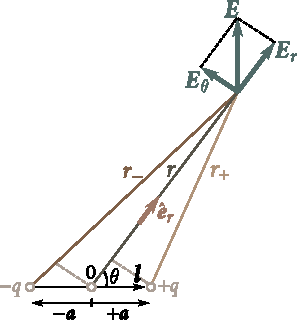
\includegraphics[scale=0.95]{figures/ch_01/fig_1_9.pdf}
			\caption[]{}
			\label{fig:1_9}
		\end{center}
	\end{minipage}
\vspace{-0.4cm}
\end{figure}

Mặt đẳng thế của trường đều là tập hợp các mặt phẳng xếp đều nhau, vuông góc với phương của điện trường.

\section{Lưỡng cực}\label{sec:1_9}

Một \textbf{lưỡng cực điện} được định nghĩa là một hệ hai điện tích điểm $+q$ và $-q$ giống nhau về giá trị và trái dấu, khoảng cách giữa hai điện tích nhỏ hơn rất nhiều so với khoảng cách tới điểm mà trường của hệ đang được quan sát . Đường thẳng đi qua cả hai điện tích gọi là  \textbf{trục lưỡng cực}.

Đầu tiên chúng ta hãy tính điện thế và sau đó là cường độ trường của một lưỡng cực. Trường này có tính đối xứng trục. Do đó, đường sức của trường trong bất kỳ mặt phẳng nào đi qua trục lưỡng cực phải giống nhau, vector $\vec{E}$ nằm trong mặt phẳng này. Vị trí của một điểm so với lưỡng cực được đặc trưng bởi vector vị trí $\vec{r}$ hoặc bởi tọa độ cực $r$ và $\theta$ (\fig{1_9}). Đặt vector $\vec{l}$ có hướng từ điện tích âm tới điện tích dương. Vị trí của điện tích  $+q$ tới tâm của lưỡng cực được xác định bởi vector $\vec{a}$, và của điện tích $-q$ là vector $-\vec{a}$. Hiển nhiên rằng $\vec{l}=2\vec{a}$. Chúng ta sẽ chỉ định khoảng cách tới một điểm cho trước từ $+q$ và $-q$ tương ứng là $r_+$ và $r_-$.

Do $a$ rất nhỏ so với $r$, chúng ta có thể tính xấp xỉ
\begin{equation}\label{eq:1_47}
\begin{split}
	r_+ &= r - a\cos\theta = r - \vec{a}\!\vec{\cdot}\!\vecuni{r},\\
	r_- &= r + a\cos\theta = r + \vec{a}\!\vec{\cdot}\!\vecuni{r}.
\end{split}
\end{equation}

Điện thế tại một điểm xác định bởi vector vị trí $\vec{r}$ là
\begin{equation*}
	\varphi(\vec{r}) = \frac{1}{4\pi\varepsilon_0} \parenthesis{
	\frac{q}{r_+} - \frac{q}{r_-}
	} = \frac{1}{4\pi\varepsilon_0} \frac{q(r_- - r_+)}{r_+ r_-}.
\end{equation*}

\noindent
$r_+r_-$ có thể thay thế bằng $r^2$. Hiệu $r_--r_+$ theo Eqs. \eqref{eq:1_47}, là $2(\vec{a}\!\vec{\cdot}\!\vecuni{r})=\vec{l}\!\vec{\cdot}\!\vecuni{r}$. Từ đó,
\begin{equation}\label{eq:1_48}
	\varphi(\vec{r}) = \frac{1}{4\pi\varepsilon_0} \frac{q(\vec{l}\!\vec{\cdot}\!\vecuni{r})}{r^2} = \frac{1}{4\pi\varepsilon_0} \frac{(\vec{p}\!\vec{\cdot}\!\vecuni{r})}{r^2}
\end{equation}

\noindent
Với
\vspace{-5pt}
\begin{equation}\label{eq:1_49}
	\vec{p} = q\vec{l}
\end{equation}

\noindent
là một đặc trưng của một lưỡng cực gọi là \textbf{moment điện}. vector $\vec{p}$ hướng dọc theo trục lưỡng cực từ điện tích âm tới điện tích dương (\fig{1_10}).

\begin{figure}[!htb]
	\begin{center}
		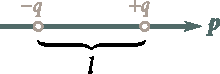
\includegraphics[scale=1]{figures/ch_01/fig_1_10.pdf}
		\caption[]{}
		\label{fig:1_10}
	\end{center}
	\vspace{-0.85cm}
\end{figure}

\eqn{1_48} chỉ ra rằng trường của một lưỡng cực được xác định bởi moment điện của nó $\vec{p}$. Chúng ta sẽ thấy lúc sau rằng biểu hiện của một lưỡng cực trong một điện trường ngoài cũng được xác định bởi moment điện của nó $\vec{p}$. So sánh với \eqn{1_26} chỉ ra rằng điện thế của của một trường lưỡng cực giảm nhanh theo khoảng cách ($1/r^2$) hơn thế năng của một trường điện tích điểm (thay đổi tỷ lệ với $1/r$).

Có thể thấy từ \fig{1_9} rằng $\vec{p}\!\vec{\cdot}\!\vecuni{r}=p\cos\theta$. Do đó, \eqn{1_48} có thể được viết như sau:
\begin{equation}\label{eq:1_50}
	\varphi(r,\theta) = \frac{1}{4\pi\varepsilon_0} \frac{p\cos\theta}{r^2}.
\end{equation}

Để tìm cường độ trường của một lưỡng cực, chúng ta hãy tính hình chiếu của vector $\vec{E}$ theo hai hướng vuông góc với nhau bởi \eqn{1_44}. Một trong số chúng được xác định bởi chuyển động của một điểm do sự thay đổi khoảng cách $r$ (với $\theta$ không đổi), cái còn lại là bởi chuyển động của điểm do thay đổi góc $\theta$ (với $r$ không đổi, xem \fig{1_9}). Hình chiếu đầu tiên nhận được bằng cách vi phân \eqn{1_50} theo $r$:
\begin{equation}\label{eq:1_51}
	E_r = - \diffpartial{\varphi}{r} = \frac{1}{4\pi\varepsilon_0} \frac{2p\cos\theta}{r^3}.
\end{equation}

\noindent
Chúng ta sẽ tìm hình chiếu thứ hai (chúng ta hãy gọi nó là  $E_{\theta}$) bằng cách lấy tỷ lệ giữa sự tăng điện thế $\varphi$ nhận được khi góc $\theta$ tăng một lượng $\deriv{\theta}$ với quãng đường $r\,\deriv{\theta}$ mà ngọn của đoạn $r$ di chuyển được (trong trường hợp này đại lượng $\deriv{l}$ trong \eqn{1_44} bằng với $r\,\deriv{\theta}$). Do đó,
\begin{equation*}
	E_{\theta} = - \frac{1}{r}\diffpartial{\varphi}{\theta}.
\end{equation*}

\noindent
Tính giá trị đạo hàm của hàm số \eqref{eq:1_50} theo $\theta$ ta có
\begin{equation}\label{eq:1_52}
	E_{\theta} = \frac{1}{4\pi\varepsilon_0} \frac{p\sin\theta}{r^3}.
\end{equation}

\noindent
Tổng bình phương của các phương trình \eqref{eq:1_51} và \eqref{eq:1_52} cho ta bình phương của vector $\vec{E}$ (xem \fig{1_9}):
\begin{align*}
	E^2 &= E_r^2 + E_{\theta}^2 = \parenthesis{\frac{1}{4\pi\varepsilon_0}}^2 \parenthesis{\frac{p}{r^3}}^2 \parenthesis{4\cos^2\theta + \sin^2\theta}\\
		&= \parenthesis{\frac{1}{4\pi\varepsilon_0}}^2 \parenthesis{\frac{p}{r^3}}^2 \parenthesis{1 + 3\cos^2\theta}.
\end{align*}

\noindent
Từ đó
\begin{equation}\label{eq:1_53}
	E = \frac{1}{4\pi\varepsilon_0} \frac{p}{r^3} \parenthesis{1 + 3\cos^2\theta}^{1/2}.
\end{equation}

Giả sử trong \eqn{1_53} $\theta=0$, chúng ta được cường độ trên trục lưỡng cực:
\begin{equation}\label{eq:1_54}
	E_{\parallel} = \frac{1}{4\pi\varepsilon_0} \frac{2p}{r^3}.
\end{equation}

\noindent
Vector $\vec{E}_{\parallel}$ hướng dọc theo trục lưỡng cực. Điều này phù hợp với tính đối xứng của bài toán. Kiểm tra \eqn{1_51} chỉ ra rằng $E_r>0$ khi $\theta=0$, và $E_r<0$ khi $\theta=\pi$. Điều này biểu thị rằng trong mọi trường hợp, vector $\vec{E}_{\parallel}$ có hướng trùng với hướng từ $-q$ tới $+q$ (tức là với hướng của $\vec{p}$). Phương trình \eqref{eq:1_54} do đó có thể viết ở dạng vector:
\begin{equation}\label{eq:1_55}
	\vec{E}_{\parallel} = \frac{1}{4\pi\varepsilon_0} \frac{2\vec{p}}{r^3}.
\end{equation}

Giả sử trong \eqn{1_53} $\theta=\pi/2$, chúng ta được cường độ trường trên đường thẳng đi qua tâm lưỡng cực và vuông góc với trục của nó:
\begin{equation}\label{eq:1_56}
	E_{\perp} = \frac{1}{4\pi\varepsilon_0} \frac{p}{r^3}.
\end{equation}

\noindent
Từ \eqn{1_51}, khi $\theta=\pi/2$, hình chiếu $E_r$ bằng không. Từ đó, vector $\vec{E}_{\perp}$ song song với trục lưỡng cực. Từ \eqn{1_52}, khi $\theta=\pi/2$, hình chiếu $E_{\theta}$ là dương. Điều này biểu thị rằng vector $\vec{E}_{\perp}$ hướng theo chiều tăng của góc $\theta$, tức là trực đối với vector $\vec{p}$.

Cường độ trường của một lưỡng cực được đặc trưng bởi sự giảm theo khoảng cách tỷ lệ với $1/r^3$, tức là giảm nhanh hơn so với cường độ trường của một điện tích điểm (giảm tỷ lệ với $1/r^2$).

\begin{figure}[!htb]
	\begin{minipage}[t]{0.5\linewidth}
		\begin{center}
			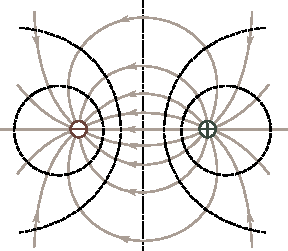
\includegraphics[scale=1]{figures/ch_01/fig_1_11.pdf}
			\caption[]{}
			\label{fig:1_11}
		\end{center}
	\end{minipage}
	\hspace{-0.05cm}
	\begin{minipage}[t]{0.5\linewidth}
		\begin{center}
			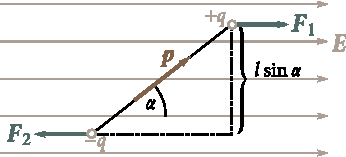
\includegraphics[scale=1]{figures/ch_01/fig_1_12.pdf}
			\caption[]{}
			\label{fig:1_12}
		\end{center}
	\end{minipage}
\vspace{-0.4cm}
\end{figure}

Hình \ref{fig:1_11} cho thấy đường $\vec{E}$ (các đường nét liền) và mặt đẳng thế (các đường nét đứt) của một trường lưỡng cực. Theo \eqn{1_50}, khi $\theta=\pi/2$, điện thế biến mất với mọi $r$. Do đó, mọi điểm thuộc mặt phẳng vuông góc với trục lưỡng cực và đi qua tâm của nó có điện thế bằng không. Điều này có thể dễ đoán bởi vì khoảng cách từ điện tích $+q$ và $-q$ tới bất kì điểm nào thuộc mặt phẳng này là như nhau.

Bây giờ chúng ta hãy xem xét biểu hiện của một lưỡng cực trong một điện trường ngoài. Nếu lưỡng cực được đặt trong một điện trường đều, điện tích $+q$ và $-q$ của lưỡng cực sẽ chịu tác dụng của lực $\vec{F}_1$ và $\vec{F}_2$ có độ lớn bằng nhau, nhưng có hướng ngược nhau (\fig{1_12}). Các lực này tạo thành một cặp có cánh tay đòn là $l\sin\alpha$, tức là phụ thuộc vào định hướng của lưỡng cực trong điện trường. Độ lớn của mỗi lực là $qE$. Nhân nó với cánh tay đòn, chúng ta nhận được độ lớn của moment ngẫu lực tác dụng lên lưỡng cực:
\begin{equation}\label{eq:1_57}
	T = q E l \sin\alpha = p E \sin\alpha
\end{equation}

\noindent
($p$ là moment điện của lưỡng cực). Dễ thấy rằng \eqn{1_57} có thể được viết ở dạng vector
\begin{equation}\label{eq:1_58}
	\vec{T} = \vecprod{p}{E}.
\end{equation}

\noindent
Moment ngẫu lực \eqref{eq:1_58} có khuynh hướng làm quay lưỡng cực sao cho moment điện $\vec{p}$ cùng hướng với trường.

Chúng ta hãy tìm thế năng của lưỡng cực trong điện trường ngoài. Theo \eqn{1_29}, năng lượng này là
\begin{equation}\label{eq:1_59}
	\ab{W}{p} = q\varphi_+ - q\varphi_- = q(\varphi_+ - \varphi_-).
\end{equation}

\noindent
ở đây $\varphi_+$ và $\varphi_-$ là giá trị của điện thế của trường ngoài tại điểm mà $+q$ và $-q$ được đặt.

Điện thế của một trường đều giảm tuyến tính theo hướng của vector $\vec{E}$. Giả sử rằng trục $x$ chỉ hướng này (\fig{1_13}), chúng ta có thể viết $E=E_x=-\diffin{\varphi}{x}$. Xem qua \fig{1_13} chỉ ra rằng hiệu $\varphi_+-\varphi_-$ bằng với độ tăng điện thế trên đoạn $\Delta{x}=l\cos\alpha$:
\begin{equation*}
	\varphi_+ - \varphi_- = \diff{\varphi}{x} l\cos\alpha = -El\cos\alpha.
\end{equation*}

\begin{figure}[!htb]
	\begin{minipage}[t]{0.5\linewidth}
		\begin{center}
			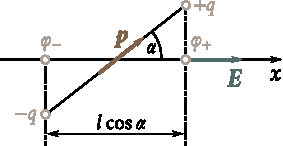
\includegraphics[scale=1]{figures/ch_01/fig_1_13.pdf}
			\caption[]{}
			\label{fig:1_13}
		\end{center}
	\end{minipage}
	\hspace{-0.05cm}
	\begin{minipage}[t]{0.5\linewidth}
		\begin{center}
			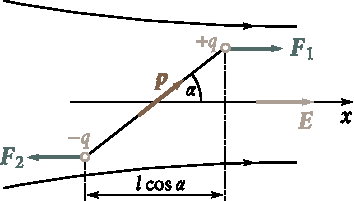
\includegraphics[scale=1]{figures/ch_01/fig_1_14.pdf}
			\caption[]{}
			\label{fig:1_14}
		\end{center}
	\end{minipage}
\vspace{-0.4cm}
\end{figure}

\noindent
Thay giá trị này vào \eqn{1_59}, ta thấy
\begin{equation}\label{eq:1_60}
	\ab{W}{p} = - q E l \cos\alpha = - p E \cos\alpha.
\end{equation}

\noindent
Ở đây $\alpha$ là góc giữa vector $\vec{p}$ và $\vec{E}$. Do đó, chúng ta có thể viết \eqn{1_60} ở dạng
\begin{equation}\label{eq:1_61}
	\ab{W}{p} = - \vecdot{p}{E}.
\end{equation}

\noindent
Chúng ta phải lưu ý rằng biểu thức này không tính đến năng lượng tương tác của các điện tích $+q$ và $-q$ tạo thành lưỡng cực.

Chúng ta đã thu được \eqn{1_61} giả sử đơn giản hóa rằng trường là đều. Tuy nhiên, phương trình này vẫn đúng cho trường không đều.

Chúng ta hãy xét lưỡng cực trong trường không đều đối xứng theo trục $x$\footnote{Một trường hợp cụ thể của một trường như vậy là của một điện tích điểm nếu chúng ta lấy một đường thẳng đi qua điện tích như là trục $x$.}. Hãy đặt tâm của lưỡng cực trên trục này, moment lưỡng cực điện làm với trục một góc $\alpha$, khác $\pi/2$ (\fig{1_14}). Trong trường hợp này, lực tác dụng lên các điện tích lưỡng cực là không giống nhau về độ lớn. Do đó, ngoài moment quay (moment ngẫu lực), lưỡng cực sẽ chịu một lực có xu hướng kéo nó theo hướng của trục $x$. Để tìm giá trị của lực này, chúng ta sử dụng \eqn{1_40}, theo đó
\begin{equation*}
	F_x = -\diffpartial{\ab{W}{p}}{x},\quad F_y = -\diffpartial{\ab{W}{p}}{y},\quad F_z = -\diffpartial{\ab{W}{p}}{z}.
\end{equation*}

\noindent
Theo \eqn{1_60}, có thể viết
\begin{equation*}
	\ab{W}{p}(x,y,z) = -p E(x,y,z)\cos\alpha
\end{equation*}

\noindent
(xem hướng của lưỡng cực so với vector $\vec{E}$ là không đổi, $\alpha=\text{constant}$).

Với các điểm nằm trên trục $x$, đạo hàm của $E$ theo $y$ và $z$ bằng không. Do đó, $\diffinpartial{\ab{W}{p}}{y}=\diffinpartial{\ab{W}{p}}{z}=0$. Vì vậy, Chỉ có thành phần lực $F_x$ khác không. 
\begin{equation}\label{eq:1_62}
	F_x = - \diffpartial{\ab{W}{p}}{x} = p \diffpartial{E}{x} \cos\alpha.
\end{equation}

\noindent
Kết quả này có thể nhận được nếu chúng ta sử dụng sự thật rằng cường độ trường tại các điểm đặt điện tích $+q$ và $-q$ (xem \fig{1_14}) khác một lượng $(\diffinpartial{E}{x})l\cos\alpha$. Theo đó, sự khác biệt giữa các lực tác dụng lên các điện tích là $q(\diffinpartial{E}{x})l\cos\alpha$, giống với \eqn{1_62}.

Khi $\alpha$ nhỏ hơn $\pi/2$, giá trị của $F_x$ xác định bởi \eqn{1_62} là dương. Điều này nói rằng dưới tác dụng của lực thì lưỡng cực bị kéo về vùng có trường mạnh hơn (xem \fig{1_14}). Khi $\alpha$ lớn hơn $\pi/2$, lưỡng cực bị đẩy khỏi trường.

\begin{figure}[!htb]
	\begin{center}
		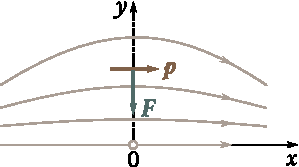
\includegraphics[scale=1]{figures/ch_01/fig_1_15.pdf}
		\caption[]{}
		\label{fig:1_15}
	\end{center}
	\vspace{-0.8cm}
\end{figure}

Ở trường hợp trong \fig{1_15}, chỉ có đạo hàm $\diffinpartial{E}{y}$ khác không cho các điểm trên trục $y$. Do đó, lực tác dụng lên lưỡng cực được xác định bởi thành phần
\begin{equation*}
	F_y = -\diffpartial{\ab{W}{p}}{y} = p \diffpartial{E}{y},\quad (\cos\alpha=1).
\end{equation*}

\noindent
Đạo hàm $\diffinpartial{E}{y}$ âm. Kết quả là, lực có hướng như trong hình. Do đó, trong trường hợp này cũng vậy, lưỡng cực bị kéo về phía trường   .

Lưu ý rằng $-\diffinpartial{\ab{W}{p}}{x}$ cho hình chiếu của lực tác dụng lên hệ theo trục $x$, còn đạo hàm \eqn{1_60} theo $\alpha$ với dấu trừ cho hình chiếu của moment ngẫu lực trên "trục" $\alpha$: $T_{\alpha}=-pE\sin\alpha$. Dấu trừ ở đây là bởi vì "trục" $\alpha$ và moment ngẫu lực $T$ có hướng ngược nhau (xem \fig{1_12}).

\section{Trường của hệ điện tích ở khoảng cách xa}\label{sec:1_10}

Xét hệ $N$ điện tích $q_1, q_2, \ldots, q_N$ trong một thể tích có kích thước $l$, và tìm hiểu về trường tạo ra bởi hệ này tại khoảng cách $r$ rất lớn so với $l$ ($r>l$). Đặt gốc tọa độ $O$ bên trong thể tích chiếm bởi hệ và xác định vị trí của các điện tích bằng các vector vị trí $\vec{r}_i$, (\fig{1_16}; để đơn giản hóa hình ảnh, chúng ta chỉ biểu diễn vector vị trí của điện tích thứ $i$).

\begin{figure}[!htb]
	\begin{center}
		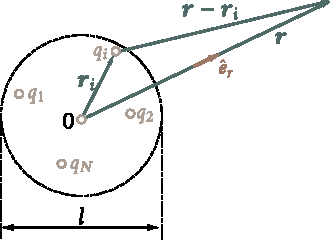
\includegraphics[scale=0.95]{figures/ch_01/fig_1_16.pdf}
		\caption[]{}
		\label{fig:1_16}
	\end{center}
	\vspace{-1.0cm}
\end{figure}

Điện thế tại điểm xác định bởi vector vị trí $\vec{r}$ là
\begin{equation}\label{eq:1_63}
	\varphi(\vec{r}) = \frac{1}{4\pi\varepsilon_0} \sum_{i=1}^N \frac{q_i}{\absolute{\vec{r} - \vec{r}_i}}.
\end{equation}

\noindent
Do $r_i$ rất nhỏ so với $r$, ta có thể cho rằng
\begin{equation*}
	\absolute{\vec{r} - \vec{r}_i} = r - \vec{r}_i\!\vec{\cdot}\!\vecuni{r} = r\parenthesis{1 - \frac{\vec{r}_i\!\vec{\cdot}\!\vecuni{r}}{r}}
\end{equation*}

\noindent
[so sánh với phương trình \eqref{eq:1_47}]. Thay biểu diễn này vào \eqn{1_63} dẫn đến
\begin{equation}\label{eq:1_64}
	\varphi(\vec{r}) = \frac{1}{4\pi\varepsilon_0} \sum_{i=1}^N \frac{q_i}{r} \bracket{\frac{1}{1 - \parenthesis{\vec{r}_i\!\vec{\cdot}\!\vecuni{r}/r}}}.
\end{equation}

\noindent
Sử dụng công thức
\begin{equation*}
	\frac{1}{1-x} \approx 1 + x
\end{equation*}

\noindent
Với $x\ll 1$, ta có thể biến đổi \eqn{1_64} như sau:
\begin{align}
	\varphi(\vec{r}) &= \frac{1}{4\pi\varepsilon_0} \sum_{i=1}^N \frac{q_i}{r} \parenthesis{1 + \frac{\vec{r}_i\!\vec{\cdot}\!\vecuni{r}}{r}}\nonumber\\
	&= \frac{1}{4\pi\varepsilon_0} \frac{1}{r} \sum_{i=1}^N q_i + \frac{1}{4\pi\varepsilon_0} \frac{1}{r^2} \parenthesis{\sum_{i=1}^N q_i \vec{r}_i}\!\vec{\cdot}\!\vecuni{r}. \label{eq:1_65}
\end{align}

\noindent
Số hạng đầu tiên của biểu thức nhận được là điện thế của trường của một điện tích điểm có giá trị $q=\sum_iq_i$ [so sánh với \eqn{1_26}]. Số hạng thứ hai có dạng giống như biểu thức xác định điện thế của một trường lưỡng cực, phần moment điện của lưỡng cực được thay bởi lượng
\begin{equation}\label{eq:1_66}
	\vec{p} = \sum_{i=1}^N q_i \vec{r}_i.
\end{equation}

\noindent
Đại lượng này được gọi là \textbf{moment lưỡng cực điện} của hệ điện tích. Dễ để xác nhận rằng đối với một lưỡng cực \eqn{1_66} biến đổi thành biểu thức $\vec{p}=q\vec{l}$ mà chúng ta đã rất quen thuộc.

\begin{figure}[!htb]
	\begin{minipage}[t]{0.4\linewidth}
		\begin{center}
			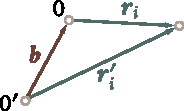
\includegraphics[scale=1]{figures/ch_01/fig_1_17.pdf}
			\caption[]{}
			\label{fig:1_17}
		\end{center}
	\end{minipage}
	\hspace{-0.05cm}
	\begin{minipage}[t]{0.6\linewidth}
		\begin{center}
			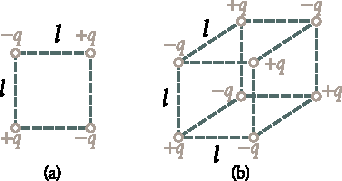
\includegraphics[scale=1]{figures/ch_01/fig_1_18.pdf}
			\caption[]{}
			\label{fig:1_18}
		\end{center}
	\end{minipage}
\vspace{-0.4cm}
\end{figure}

Nếu tổng điện tích của hệ bằng không ($\sum_iq_i=0$), giá trị của moment lưỡng cực không phụ thuộc vào việc chọn gốc tọa độ. Để giải thích việc này, chọn hai gốc tọa độ tùy ý $O$ và $O'$ (\fig{1_17}). Vector vị trí của điện tích thứ $i$ từ các điểm này liên hệ như sau:
\begin{equation}\label{eq:1_67}
	\vec{r}_i' = \vec{b} + \vec{r}_i
\end{equation}

\noindent
(vector $\vec{b}$ như trong hình).Với \eqn{1_67}, moment lưỡng cực trong hệ có gốc $0'$ là
\begin{equation*}
	\vec{p}' = \sum_i q_i \vec{r}_i = \sum_i q_i (\vec{b} + \vec{r}_i) = \vec{b} \sum_i q_i + \sum_i q_i \vec{r}_i.
\end{equation*}

\noindent
Số hạng đầu tiên bằng không (vì $\sum_iq_i=0$). Số hạng thứ hai là $\vec{p}$---moment lưỡng cực trong hệ tọa độ có gốc $O$. Do đó $\vec{p}'=\vec{p}$.

Phương trình \eqref{eq:1_65} về bản chất là hai số hạng đầu tiên của chuỗi khai triển của hàm số \eqref{eq:1_63} thành lũy thừa của $r_i/r$. Khi $\sum_iq_i\neq 0$, số hạng đầu tiên của \eqn{1_65} đóng góp chính vào điện thế (số hạng thứ hai giảm tỷ lệ với $1/r^2$ và do đó nhỏ hơn rất nhiều so với cái đầu tiên). Với một hệ trung hòa điện ($\sum_iq_i=0$), số hạng đầu tiên bằng không, và điện thế được xác định chủ yếu bởi số hạng thứ hai của \eqn{1_65}. Đây là cách mọi việc diễn ra, đặc biệt, cho trường của một lưỡng cực.

Với hệ điện tích mô tả trong \fig{1_18}a được gọi là một \textbf{tứ cực}, cả $\sum_iq_i$ và $\vec{p}$ bằng không, do đó \eqn{1_65} cho điện thế bằng không. Thật ra, trường của một tứ cực, mặc dù nó yếu hơn nhiều so với lưỡng cực (với cùng giá trị của $q$ và $l$), nhưng khác không. Điện thế của trường tạo ra bởi tứ cực được xác định chủ yếu bởi số hạng thứ ba của khai triển tỷ lệ với $1/r^3$. Để nhận được số hạng này, chúng ta phải tính đến đại lượng $(r_i/r)^2$ mà chúng ta đã bỏ qua khi dẫn đến \eqn{1_65}. Với hệ điện tích trong \fig{1_18}b gọi là một \textbf{bát cực}, số hạng thứ ba của khai triển cũng bằng không. Điện thế của trường như vậy được xác định bởi số hạng thứ tư của khai triển, tỷ lệ với $1/r^4$.

Cần lưu ý rằng đại lượng bằng với $\sum_iq_i$ ở tử số của số hạng đầu tiên của \eqn{1_65} được gọi là một \textbf{đơn cực} hoặc một \textbf{đa cực bậc không}, một lưỡng cực cũng được gọi là một \textbf{đa cực bậc một}, một tứ cực được gọi là một \textbf{đa cực bậc hai}, vân vân.

Do đó, trong trường hợp tổng quát, trường của một hệ điện tích tại khoảng cách xa có thể được biểu diễn như là sự chồng chất của các trường tạo bởi đa cực thuộc các cấp khác nhau---đơn cực, lưỡng cực, tứ cực, bát cực, vân vân.

\section{Mô tả các thuộc tính của trường vector}\label{sec:1_11}

Để tiếp tục nghiên cứu điện trường, chúng ta phải làm quen với các công cụ toán học sử dụng để mô tả các tính chất của trường vector. Các công cụ này được gọi là \textbf{phân tích vector}. Trong phần này, ta sẽ xem xét các khái niệm cơ bản và các công thức chọn lọc của phân tích vector, và cũng chứng minh hai định lý chính của nó---định lý Ostrogradsky-Gauss (hoặc là định lý phân kỳ Gauss) và định lý Stokes.

Các đại lượng sử dụng trong phân tích vector có thể được minh họa tốt nhất bởi trường vector vận tốc của chất lỏng đang chảy. Do đó ta đưa ra các đại lượng này khi xử lý với dòng chất lỏng lý tưởng không nén, và sau đó mở rộng kết quả nhận được cho trường vector có bản chất bất kỳ.

Chúng ta đã quen với một trong những khái niệm của phân tích vector. Đó là \textbf{gradient}, sử dụng để mô tả các trường vô hướng. Nếu giá trị của đại lượng vô hướng $\varphi=\varphi(x, y, z)$ gán cho mọi điểm P có tọa độ $x, y, z$, ta nói rằng trường vô hướng của $\varphi$ được thiết lập. Gradient của đại lượng $\varphi$ được định nghĩa là vector
\begin{equation}\label{eq:1_68}
	\grad{\varphi} = \diffpartial{\varphi}{x}\,\vecuni{x} + \diffpartial{\varphi}{y}\,\vecuni{y} + \diffpartial{\varphi}{z}\,\vecuni{z}.
\end{equation}

Độ tăng của hàm $\varphi$ khi dịch chuyển trên chiều dài $\deriv{\vec{l}}=\vecuni{x}\,\deriv{x}+\vecuni{y}\,\deriv{y}+\vecuni{z}\,\deriv{z}$ là
\begin{equation*}
	\deriv{\varphi} = \diffpartial{\varphi}{x}\,\deriv{x} + \diffpartial{\varphi}{y}\,\deriv{y} + \diffpartial{\varphi}{z}\,\deriv{z}
\end{equation*}

\noindent
Có thể viết ở dạng
\begin{equation}\label{eq:1_69}
	\deriv{\varphi} = \grad{\varphi} \ccdot \deriv{\vec{l}}.
\end{equation}

Bây giờ ta sẽ chuyển sang thiết lập các đặc tính của trường vector.

\begin{figure}[!htb]
	\begin{center}
		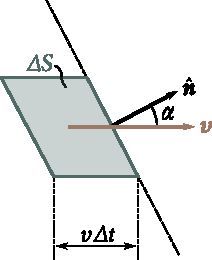
\includegraphics[scale=1]{figures/ch_01/fig_1_19.pdf}
		\caption[]{}
		\label{fig:1_19}
	\end{center}
	\vspace{-0.8cm}
\end{figure}

\textbf{Thông lượng vector.} Giả sử rằng dòng chảy chất lỏng được đặc trưng bởi trường vector vận tốc. Lượng chất lỏng chảy qua một bề mặt tưởng tượng $S$ trong đơn vị thời gian gọi là thông lượng của chất lỏng qua bề mặt này. Để tìm thông lượng, ta chia bề mặt thành các phần nguyên tố có kích thước $\Delta{S}$. Có thể thấy từ \fig{1_19} rằng trong thời gian $\Delta{t}$ lượng chất lỏng bằng
\begin{equation*}
	\Delta{V} = (\Delta{S}\cos\alpha) v\Delta{t}
\end{equation*}

\noindent
sẽ đi qua phần tử $\Delta{S}$. Chia thể tích này với thời gian $\Delta{t}$, ta sẽ tìm được thông lượng qua mặt $\Delta{S}$:
\begin{equation*}
	\Delta{\Phi} = \frac{\Delta{V}}{\Delta{t}} = \Delta{S} v \cos\alpha.
\end{equation*}

\noindent
Chuyển qua vi phân, ta được
\begin{equation}\label{eq:1_70}
	\deriv{\Phi} = (v \cos\alpha)\, \deriv{S}.
\end{equation}

\noindent
Phương trình \eqref{eq:1_70} có thể viết trong hai cách khác nhau. Cách đầu tiên, nếu chúng ta tính đến $v\cos\alpha$ là hình chiếu của vector vận tốc lên pháp tuyến $\vecuni{n}$ của diện tích $\deriv{S}$, ta có thể viết \eqn{1_70} ở dạng
\begin{equation}\label{eq:1_71}
	\deriv{\Phi} = v_n\, \deriv{S}.
\end{equation}

\noindent
Cách thứ hai, ta đưa vào vector $\deriv{\vec{S}}$ có độ lớn bằng diện tích $\deriv{S}$, trong khi hướng của nó trùng với hướng của pháp tuyến $\hatvec{n}$ của diện tích:
\begin{equation*}
	\deriv{\vec{S}} = \deriv{S}\, \hatvec{n}.
\end{equation*}

\noindent
Vì hướng của vector $\hatvec{n}$ được chọn tùy ý (nó có thể là một trong hai bên của diện tích), nên $\deriv{\vec{S}}$ không phải một vector thực, mà là một giả vector. Góc $\alpha$ trong \eqn{1_70} là góc giữa vector $\vec{v}$ và $\deriv{\vec{S}}$. Từ đó, phương trình này có thể được viết ở dạng
\begin{equation}\label{eq:1_72}
	\deriv{\Phi} = \vec{v} \ccdot \deriv{\vec{S}}.
\end{equation}

Bằng cách lấy tổng thông lượng qua tất cả diện tích nguyên tố được chia ra từ bề mặt $S$, ta được thông lượng của chất lỏng qua $S$:
\begin{equation}\label{eq:1_73}
	\Phi_v = \int_S \vec{v} \ccdot \deriv{\vec{S}} = \int_S v_n\, \deriv{S}.
\end{equation}

\noindent
Một biểu thức tương tự cho một trường vector $\vec{a}$ tùy ý, nghĩa là lượng
\begin{equation}\label{eq:1_74}
	\Phi_a = \int_S \vec{a} \ccdot \deriv{\vec{S}} = \int_S a_n\, \deriv{S}
\end{equation}

\noindent
được gọi là \textbf{thông lượng của vector a qua bề mặt} $S$. Theo định nghĩa này, thông lượng của chất lỏng có thể gọi là thông lượng của vector $\vec{v}$ qua bề mặt đã cho [xem \eqn{1_73}].

Thông lượng của một vector là một đại lượng đại số. Dấu của nó phụ thuộc vào việc chọn hướng của pháp tuyến phần tử diện tích được chia ra từ bề mặt $S$ trong tính thông lượng. Đảo hướng của pháp tuyến làm đổi dấu của $a_n$ và, do đó, là dấu của đại lượng \eqref{eq:1_74}. Cách làm thông thường cho mặt kín là tính thông lượng ``hướng ra ngoài'' vùng bên trong bề mặt. Do đó, trong phần sau ta sẽ luôn ngụ ý rằng $\hatvec{n}$ là một ngoại hướng pháp tuyến.

\begin{figure}[!htb]
	\begin{center}
		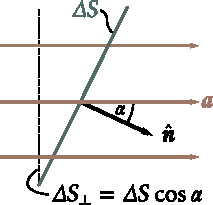
\includegraphics[scale=0.95]{figures/ch_01/fig_1_20.pdf}
		\caption[]{}
		\label{fig:1_20}
	\end{center}
	\vspace{-1.0cm}
\end{figure}

Ta có thể đưa ra một giải thích hình học minh họa cho thông lượng vector. Vì mục đích này, ta sẽ biểu diễn một trường vector bằng một hệ các đường sức $\vec{a}$ được dựng sao cho mật độ các đường sức tại mỗi điểm có trị số bằng với độ lớn của vector $\vec{a}$ tại điểm đó trong trường (so sánh với quy tắc xây dựng các đường sức của vector $\vec{E}$ được nêu ở cuối \sect{1_5}). Ta hãy tìm số giao điểm $\Delta{N}$ của đường sức trường với diện tích ảo $\Delta{S}$. \fig{1_20} chỉ ra rằng số này bằng mật độ đường sức (tức là $a$) nhân với $\Delta{S}_{\perp}=\Delta{S}\cos\alpha$:
\begin{equation*}
	\Delta{N}\, (=)\, a \Delta{S}\cos\alpha = a_n \Delta{S}.
\end{equation*}

\noindent
Ta chỉ nói sự bằng nhau về chỉ số giữa $\Delta{N}$ và $a_n\Delta{S}$. Đó là lý do tại sao dấu bằng nằm trong ngoặc đơn. Theo \eqn{1_74}, biểu thức $a_n\Delta{S}$ là $\Delta{\Phi}$---thông lượng vector qua diện tích $\Delta{S}$. Do đó,
\begin{equation}\label{eq:1_75}
	\Delta{N}\, (=)\, \Delta{\Phi}_a.
\end{equation}

Để dấu của $\Delta{N}$ trùng với dấu của $\Delta{\Phi}_a$, ta phải xem số giao điểm là dương khi góc $\alpha$ giữa chiều dương của đường sức trường và pháp tuyến của diện tích là góc nhọn. Giao điểm được coi là âm nếu góc $\alpha$ là góc tù. Với diện tích trong \fig{1_20}, cả ba giao điểm là dương: $\Delta{N}=+3$ ($\Delta{\Phi}_a$ trong trường hợp này cũng dương vì $a_n>0$). Nếu hướng của pháp tuyến trong \fig{1_20} đảo chiều, giao điểm sẽ trở thành âm ($\Delta{N}=-3$), và thông lượng $\Delta{\Phi}_a$ cũng âm.

Tính tổng của \eqn{1_75} trên bề mặt ảo hữu hạn $S$ dẫn đến
\begin{equation}\label{eq:1_76}
	\Delta{\Phi}_a\, (=)\, \sum\Delta{N} = N_+ - N_-
\end{equation}

\noindent
$N_+$ và $N_-$ lần lượt và tổng số giao điểm dương và âm của đường sức trường với bề mặt $S$.

Người đọc có thể bị rối vì thông lượng được biểu diễn bằng một phân số, số giao điểm của đường trường với bề mặt so với thông lượng cũng sẽ là phân số. Tuy nhiên, đừng nhầm lẫn điều này. Đường sức trường là một hình ảnh có điều kiện bị thiếu đi ý nghĩa vật lý.

Ta hãy lấy một bề mặt tưởng tượng dưới dạng một dải giấy có phần dưới bị xoắn so với phần trên một góc $\pi$ (\fig{1_21}). Hướng của pháp tuyến phải chọn như nhau cho toàn thể bề mặt. Từ đó, nếu ở phần trên của dải, pháp tuyến dương chỉ sang phải, thì pháp tuyến của phần dưới sẽ chỉ sang trái. Theo đó, các giao điểm của đường sức trường miêu tả trong \fig{1_21} với nửa mặt trên là dương, và với nửa dưới là âm.

\begin{figure}[!htb]
	\begin{minipage}[t]{0.4\linewidth}
		\begin{center}
			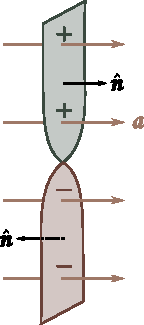
\includegraphics[scale=0.95]{figures/ch_01/fig_1_21.pdf}
			\caption[]{}
			\label{fig:1_21}
		\end{center}
	\end{minipage}
	\hspace{-0.05cm}
	\begin{minipage}[t]{0.6\linewidth}
		\begin{center}
			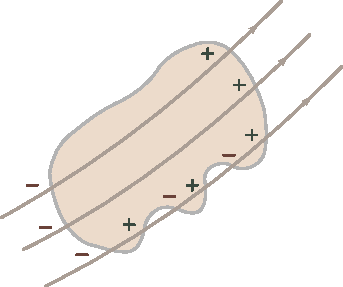
\includegraphics[scale=0.95]{figures/ch_01/fig_1_22.pdf}
			\caption[]{}
			\label{fig:1_22}
		\end{center}
	\end{minipage}
\vspace{-0.4cm}
\end{figure}

Ngoại hướng pháp tuyến được coi là dương với một mặt kín (\fig{1_22}). Do đó, các giao điểm ứng với các điểm mà đường sức đi ra khỏi bề mặt (góc $\alpha$ là góc nhọn) mang dấu dương, và những điểm đường sức đi vào bề mặt (góc $\alpha$ là góc tù) mang dấu âm.

Phân tích \fig{1_22} chỉ ra rằng khi các đường sức trường đi vào một mặt kín liên tục, mỗi đường khi giao nhau với bề mặt sẽ đi vào nó và đi ra khỏi nó cùng một số lượng. Kết quả là thông lượng của vector tương ứng đi qua mặt này bằng không. Dễ thấy rằng nếu đường sức trường kết thúc trong một bề mặt, thông lượng vector qua mặt kín sẽ có trị số bằng với hiệu giữa số đường sức bắt đầu bên trong bề mặt ($\ab{N}{beg}$) và số đường sức kết thúc bên trong bề mặt ($\ab{N}{term}$):
\begin{equation}\label{eq:1_77}
	\Phi_a\, (=)\, \ab{N}{beg} - \ab{N}{term}.
\end{equation}

\noindent
Dấu của thông lượng phụ thuộc vào số nào lớn hơn. Khi $\ab{N}{beg}$ bằng $\ab{N}{term}$, thông lượng bằng không.

\textbf{Divergence.} Giả sử rằng ta được cho trường vector vận tốc của một chất lỏng liên tục không nén. Ta lấy một mặt kín ảo $S$ lân cận điểm P (\fig{1_23}). Nếu trong thể tích giới hạn bởi bề mặt này không có chất lỏng xuất hiện và cũng không biến mất, thì thông lượng chảy ra ngoài qua bề mặt hiển nhiên bằng không. Thông lượng chất lỏng $\Phi_v$ khác không sẽ chỉ ra rằng có nguồn chất lỏng hoặc là phần chìm trong bề mặt, tức là, các điểm mà tại đó chất lỏng đi vào thể tích (phần chìm) hoặc thoát ra khỏi nó (nguồn). Độ lớn của thông lượng xác định tổng công suất đại số của các nguồn và các phần chìm\footnote{Công suất của một nguồn (phần chìm) được định nghĩa là thể tích chất lỏng xả ra (bị hấp thụ) trong đơn vị thời gian. Có thể coi một phần chìm như một nguồn với công suất âm.}. Khi nguồn chiếm ưu thế trước phần chìm, độ lớn của thông lượng sẽ dương, ngược lại, âm.

\begin{figure}[!htb]
	\begin{center}
		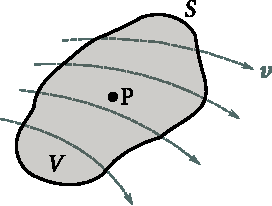
\includegraphics[scale=1]{figures/ch_01/fig_1_23.pdf}
		\caption[]{}
		\label{fig:1_23}
	\end{center}
	\vspace{-0.8cm}
\end{figure}

Thương số nhận được khi chia thông lượng $\Phi_v$ với thể tích,
\begin{equation}\label{eq:1_78}
	\frac{\Phi_v}{V}
\end{equation}

\noindent
cho công suất đơn vị trung bình của các nguồn giới hạn trong thể tích $V$. Giới hạn khi $V$ tiến tới không, tức là, thể tích $V$ co lại thành điểm P, biểu thức \eqref{eq:1_78} cho đúng công suất đơn vị của nguồn tại điểm P, gọi là \textbf{divergence} của vector $\vec{v}$ (được viết là $\diverg{\vec{v}}$). Do đó, theo định nghĩa,
\begin{equation*}
	\diverg{\vec{v}} = \lim_{V\to \text{P}} \frac{\Phi_v}{V}.
\end{equation*}

\noindent
Divergence của bất kì vector $\vec{a}$ được xác định theo cách tương tự:
\begin{equation}\label{eq:1_79}
	\diverg{\vec{a}} = \lim_{V\to \text{P}} \frac{\Phi_a}{V} = \lim_{V\to \text{P}} \frac{1}{V} \oint \vec{a} \ccdot \deriv{\vec{S}}.
\end{equation}

\noindent
Tích phân được lấy trên mặt kín $S$ tùy ý xung quanh điểm P\footnote{Vòng tròn trên dấu tích phân biểu thị rằng lấy tích phân trên một mặt kín.}; $V$ là thể tích giới hạn trong mặt này. Vì sự biến đổi $V\to$P được thực hiện khi $S$ tiến tới không, ta có thể giả sử rằng \eqn{1_79} không phụ thuộc vào hình dạng bề mặt. Giả định này được xác nhận bằng các tính toán chặt chẽ.

Ta hãy bao quanh điểm P bằng một mặt cầu có bán kính rất nhỏ $r$ (\fig{1_24}). Do $r$ rất nhỏ, thể tích $V$ bao quanh bởi hình cầu cũng sẽ rất nhỏ. Do đó với độ chính xác cao, ta có thể xem giá trị của $\diverg{\vec{a}}$ trong giới hạn của thể tích $V$ là không đổi\footnote{Giả sử rằng giá trị của $\diverg{\vec{a}}$ thay đổi liên tục, không có bước nhảy nào, khi đi từ một điểm của trường tới điểm khác.}. Trong trường hợp này, ta có thể viết phù hợp với \eqn{1_79} 
\begin{equation*}
	\Phi_a \approx (\diverg{\vec{a}}) V
\end{equation*}

\noindent
Với $\Phi_a$ là thông lượng của vector a qua bề mặt bao bọc thể tích $V$. Theo \eqn{1_77}, $\Phi_a$ bằng $\ab{N}{beg}$, số đường a bắt đầu bên trong $V$ nếu $\diverg{\vec{a}}$ tại điểm P dương, hoặc $\ab{N}{term}$, số đường a kết thúc bên trong $V$ nếu $\diverg{\vec{a}}$ tại điểm P âm.

Như trên thì các đường của vector $\vec{a}$ bắt đầu ở vùng lân cận gần một điểm nhất thì có divergence dương. Đường sức trường ``phân kỳ'' từ điểm này; ``nguồn'' của trường (\fig{1_24}a). Trái lại, trong vùng lân cận của một điểm có divergence âm, các đường của vector $\vec{a}$ kết thúc. Các đường sức trường ``hội tụ'' về điểm này; ``phần chìm'' của trường (\fig{1_24}b). Giá trị tuyệt đối của $\diverg{\vec{a}}$ càng lớn, số đường bắt đầu hoặc kết thúc ở vùng lân cận của điểm đã cho càng lớn.

Từ định nghĩa \eqref{eq:1_79} có thể thấy rằng divergence là một hàm vô hướng của tọa độ xác định vị trí các điểm trong không gian (ngắn gọn là---một hàm điểm). Định nghĩa \eqref{eq:1_79} là định nghĩa chung nhất độc lập với loại hệ tọa độ sử dụng.

\begin{figure}[!htb]
	\begin{minipage}[t]{0.5\linewidth}
		\begin{center}
			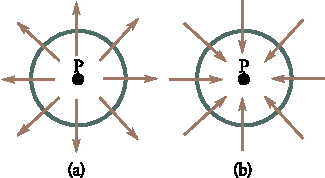
\includegraphics[scale=1.0]{figures/ch_01/fig_1_24.pdf}
			\caption[]{}
			\label{fig:1_24}
		\end{center}
	\end{minipage}
	\hspace{-0.05cm}
	\begin{minipage}[t]{0.5\linewidth}
		\begin{center}
			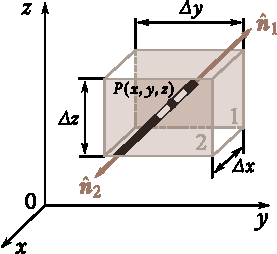
\includegraphics[scale=1.0]{figures/ch_01/fig_1_25.pdf}
			\caption[]{}
			\label{fig:1_25}
		\end{center}
	\end{minipage}
\vspace{-0.4cm}
\end{figure}

Ta hãy tìm biểu thức cho divergence trong hệ tọa độ Descartes. Xét một thể tích nhỏ dạng hình hộp với các cạnh song song với các trục tọa độ trong vùng lân cận điểm $P(x, y, z)$ (\fig{1_25}). Thông lượng vector qua mặt hình hộp được tính từ thông lượng qua từng mặt trong sáu mặt riêng lẻ.

Ta tìm thông lượng qua cặp mặt phẳng vuông góc trục $x$ (trong \fig{1_25} các mặt này được biểu diễn bằng các diện tích bóng mờ và đánh số 1 và 2). Ngoại hướng pháp tuyến $\hatvec{n}_2$ của mặt 2 trùng với hướng của trục $x$. Do đó, với các điểm trên mặt này, $a_{n_2}=a_x$. Ngoại hướng pháp tuyến $\hatvec{n}_1$ của mặt 1 ngược hướng với trục $x$. Do đó, với các điểm trên mặt này, $a_{n_1}=-a_x$. Thông lượng qua mặt 2 có thể được viết ở dạng
\begin{equation*}
	a_{x,2}\Delta{y}\Delta{z}
\end{equation*}

\noindent
với $a_{x,2}$ là giá trị trung bình của $a_x$ trên mặt 2. Thông lượng qua mặt 1 là
\begin{equation*}
	- a_{x,1}\Delta{y}\Delta{z}
\end{equation*}

\noindent
với $a_{x,1}$ là giá trị trung bình của $a_x$ trên mặt 1. Tổng thông lượng qua mặt 1 và 2 là
\begin{equation}\label{eq:1_80}
	(a_{x,2} - a_{x,1}) \Delta{y}\Delta{z}.
\end{equation}

Hiệu $a_{x,2}-a_{x,1}$ là độ tăng giá trị trung bình của $a_x$ khi dịch chuyển dọc theo trục $x$ khoảng $\Delta{x}$. Nhờ độ nhỏ của hình hộp (nhắc lại rằng ta sẽ cho kích thước của nó co lại về không), độ tăng này có thể viết ở dạng $(\diffinpartial{a_x}{x})\Delta{x}$, với giá trị $\diffinpartial{a_x}{x}$ lấy tại điểm P\footnote{Sự thiếu chính xác ta chấp nhận ở đây biến mất khi thể tích co lại thành điểm P trong biến đổi giới hạn.}. Do đó, \eqn{1_80} trở thành
\begin{equation*}
	\diffpartial{a_x}{x}\Delta{x}\Delta{y}\Delta{z} = \diffpartial{a_x}{x}\Delta{V}.
\end{equation*}

\noindent
Lập luận tương tự cho phép ta thu được các biểu thức sau cho thông lượng qua các cặp mặt vuông góc với trục $y$ và $z$:
\begin{equation*}
	\diffpartial{a_y}{y}\Delta{x}\Delta{y}\Delta{z} = \diffpartial{a_y}{y}\Delta{V},\quad \diffpartial{a_z}{z}\Delta{x}\Delta{y}\Delta{z} = \diffpartial{a_z}{z}\Delta{V}.
\end{equation*}

Do đó, thông lượng tổng cộng qua toàn bộ bề mặt kín được xác định bởi biểu thức
\begin{equation*}
	\Phi_a = \parenthesis{\diffpartial{a_x}{x} + \diffpartial{a_y}{y} + \diffpartial{a_z}{z}}\Delta{V}.
\end{equation*}

\noindent
Chia biểu thức này với $\Delta{V}$, ta sẽ tìm được divergence của vector a tại điểm $P(x, y, z)$:
\begin{equation}\label{eq:1_81}
	\diverg{\vec{a}} = \diffpartial{a_x}{x} + \diffpartial{a_y}{y} + \diffpartial{a_z}{z}.
\end{equation}

\textbf{Định lý Ostrogradsky-Gauss.} Nếu ta biết divergence của vector $\vec{a}$ tại mọi điểm trong không gian, ta có thể tính thông lượng của vector này qua mọi mặt kín có kích thước hữu hạn. Ta hãy làm điều này đầu tiên cho thông lượng vector $\vec{v}$ (thông lượng chất lỏng). Tích $\diverg{\vec{v}}$ và $\deriv{V}$ cho công suất của nguồn chất lỏng giới hạn trong thể tích $\deriv{V}$. Tổng của tích này $\int(\diverg{\vec{v}})\,\deriv{V}$, cho ta tổng công suất đại số của các nguồn giới hạn trong thể tích $V$ mà tích phân được lấy. Do chất lỏng không nén, tổng công suất của các nguồn phải bằng thông lượng chất lỏng chảy ra mặt $S$ bao quanh thể tích $V$. Vì thế ta có phương trình
\begin{equation*}
	\oint_S \vec{v} \ccdot \deriv{\vec{S}} = \int_V (\diverg{\vec{v}})\,\deriv{V}.
\end{equation*}

\noindent
Phương trình tương tự cho trường vector có bản chất bất kỳ:
\begin{equation}\label{eq:1_82}
	\oint_S \vec{a} \ccdot \deriv{\vec{S}} = \int_V (\diverg{\vec{a}})\,\deriv{V}.
\end{equation}

\noindent
Liên hệ này được gọi là định lý \textbf{Ostrogradsky-Gauss}. Tích phân bên trái được tính trên một mặt kín tùy ý $S$, và tích phân bên phải được tính trên thể tích $V$ bao bọc bởi bề mặt này.

\textbf{Lưu số.} Ta hãy trở lại với dòng chất lỏng lý tưởng không nén. Tưởng tượng một đường kín---chu tuyến $\Gamma$. Giả sử bằng một cách nào đó ta đóng băng ngay lập tức chất lỏng trong toàn bộ thể tích ngoại trừ một kênh kín rất mỏng có tiết diện không đổi bao gồm đường cong kín $\Gamma$ (\fig{1_26}). Tùy thuộc vào bản chất của trường vector vận tốc, chất lỏng trong kênh sẽ đứng yên hoặc chuyển động dọc đường cong kín (lưu thông) theo một trong hai hướng khả dĩ. Ta hãy lấy đại lượng bằng tích của vận tốc chất lỏng trong kênh và chiều dài đường cong kín $l$ như một cách đo lường chuyển động này. Đại lượng này được gọi là \textbf{lưu số} của vector $\vec{v}$ trên đường cong kín $\Gamma$. Do đó,
\begin{equation*}
	\text{lưu số của $\vec{v}$ trên $\Gamma$} = vl
\end{equation*}

\noindent
(Vì ta giả sử kênh có tiết diện không đổi, nên độ lớn của vận tốc, $v$, không đổi).

\begin{figure}[!htb]
	\begin{center}
		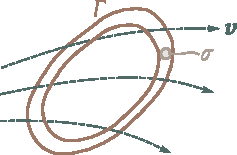
\includegraphics[scale=1]{figures/ch_01/fig_1_26.pdf}
		\caption[]{}
		\label{fig:1_26}
	\end{center}
	\vspace{-0.8cm}
\end{figure}

Tại thời điểm các bức tường đóng băng, thành phần vận tốc vuông góc với tường sẽ bị loại bỏ trong mỗi hạt chất lỏng, và chỉ còn lại thành phần vận tốc tiếp tuyến với đường cong kín $v_l$. Động lượng $\deriv{\vec{p}_l}$, gắn với thành phần này. Độ lớn của động lượng phần chất lỏng chứa trong một đoạn của kênh có chiều dài $\deriv{l}$ là $\rho\sigma v_l\,\deriv{l}$ ($\rho$ là khối lượng riêng chất lỏng, và $\sigma$ là tiết diện của kênh). Vì chất lỏng lý tưởng, tác động của các tường chỉ có thể đổi hướng vector $\deriv{\vec{p}_l}$, chứ không thay đổi độ lớn của nó. Sự sương tác giữa các hạt chất lỏng sẽ dẫn đến sự phân bố lại động lượng giữa chúng và làm cân bằng vận tốc của tất cả các hạt. Tổng đại số thành phần tiếp tuyến của động lượng không đổi: Động lượng một hạt tương tác nhận được bằng với động lượng bị mất của hạt thứ hai. Điều này chỉ ra rằng
\begin{equation*}
	\rho\sigma vl = \oint_{\Gamma} \rho \sigma v_l\,\deriv{l}
\end{equation*}

\noindent
với $v$ là vận tốc ổn định, và $v_l$ là thành phần tiếp tuyến của vận tốc chất lỏng trong thể tích $\sigma\,\deriv{l}$ tại thời điểm trước khi đóng băng. Rút gọn $\rho\sigma$, ta có
\begin{equation*}
	\text{lưu số của $\vec{v}$ trên $\Gamma$} = vl = \oint_{\Gamma} v_l\,\deriv{l}.
\end{equation*}

\noindent
Lưu số của bất kì vector $\vec{a}$ trên một đường kín tùy ý $\Gamma$ được xác định theo cách tương tự:
\begin{equation}\label{eq:1_83}
	\text{lưu số của $\vec{a}$ trên $\Gamma$} = \oint_{\Gamma} \vec{a} \ccdot \deriv{\vec{l}} = \oint_{\Gamma} a_l\,\deriv{l}.
\end{equation}

Có vẻ như khi lưu số khác không, các đường vector phải kín hoặc ít nhất bị uống cong theo cách nào đó hoặc khác theo hướng phá vỡ đường cong kín. Dễ thấy rằng giả thiết này sai. Ta hãy xét dòng chảy tầng của nước trong một con sông. Vận tốc của nước tại đáy sông bằng không và tăng dần khi ta tiếp cận mặt nước (\fig{1_27}). Đường dòng (đường vector $\vec{v}$) là đường thẳng. Mặc dù điều này, lưu số vector $\vec{v}$ trên đường cong kín minh họa bởi đường nét đứt hiển nhiên khác không. Mặt khác, trong trường có các đường cong,lưu số có thể bằng không.

\begin{figure}[!htb]
	\begin{minipage}[t]{0.5\linewidth}
		\begin{center}
			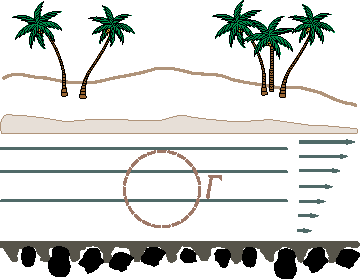
\includegraphics[scale=0.95]{figures/ch_01/fig_1_27.pdf}
			\caption[]{}
			\label{fig:1_27}
		\end{center}
	\end{minipage}
	\hspace{-0.05cm}
	\begin{minipage}[t]{0.5\linewidth}
		\begin{center}
			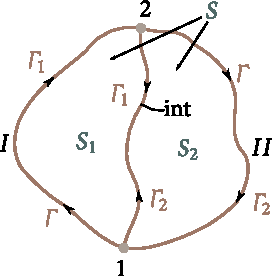
\includegraphics[scale=0.95]{figures/ch_01/fig_1_28.pdf}
			\caption[]{}
			\label{fig:1_28}
		\end{center}
	\end{minipage}
\vspace{-0.65cm}
\end{figure}

Lưu số có tính cộng. Điều này nghĩa là tổng lưu số trên đoạn $\Gamma_1$ và $\Gamma_2$ bao quanh bề mặt $S_1$ và $S_2$ (\fig{1_28}) bằng với thông lượng trên đoạn $\Gamma$ bao quanh bề mặt $S$, cái mà là ghép của bề mặt $S_1$ và $S_2$. Thật vậy, lưu số $C_1$ trên đoạn bao quanh bề mặt $S_1$ có thể biểu diễn như là tổng của các tích phân
\begin{equation}\label{eq:1_84}
	C_1 = \oint_{\Gamma_1} \vec{a} \ccdot \deriv{\vec{l}} = \int_{1,(I)}^2 \vec{a} \ccdot \deriv{\vec{l}} + \int_{2,(\text{int.})}^1 \vec{a} \ccdot \deriv{\vec{l}}.
\end{equation}

\noindent
Tích phân đầu tiên được lấy trên phần $I$ của đường bao ngoài, cái thứ hai lấy trên giao tuyến giữa mặt $S_1$ và $S_2$ theo hướng $2$-$1$.

Tương tự, lưu số $C_2$ lấy trên đoạn bao quanh bề mặt $S_2$ là
\begin{equation}\label{eq:1_85}
	C_2 = \oint_{\Gamma_2} \vec{a} \ccdot \deriv{\vec{l}} = \int_{2,(II)}^1 \vec{a} \ccdot \deriv{\vec{l}} + \int_{1,(\text{int.})}^2 \vec{a} \ccdot \deriv{\vec{l}}.
\end{equation}

\noindent
Tích phân đầu tiên được lấy trên phần $II$ của đường bao ngoài, cái thứ hai lấy trên giao tuyến giữa mặt $S_1$ và $S_2$ theo hướng $1$-$2$.

Lưu số trên đoạn giới hạn bề mặt $S$ có thể biểu diễn ở dạng
\begin{equation}\label{eq:1_86}
	C = \oint_{\Gamma} \vec{a} \ccdot \deriv{\vec{l}} = \int_{1,(I)}^2 \vec{a} \ccdot \deriv{\vec{l}} + \int_{2,(II)}^1 \vec{a} \ccdot \deriv{\vec{l}}.
\end{equation}

\noindent
Số hạng thứ hai trong phương trình \eqref{eq:1_84} và \eqref{eq:1_85} chỉ khác dấu nhau. Do đó, tổng các biểu thức này bằng \eqn{1_86}. Từ đó,
\begin{equation}\label{eq:1_87}
	C = C_1 + C_2.
\end{equation}

Phương trình \eqref{eq:1_87} ta đã chứng minh không phụ thuộc vào hình dạng bề mặt và đúng cho mọi số lượng số hạng. Từ đó, nếu ta chia một bề mặt mở $S$ tùy ý thành một lượng lớn bề mặt nguyên tố $\Delta{S}$\footnote{Trong hình, các mặt nguyên tố được mô tả ở dạng hình chữ nhật. Thực ra, hình dạng của chúng có thể hoàn toàn tùy ý.} (\fig{1_29}), thì lưu số trên đoạn bao quanh $S$ có thể viết dưới dạng tổng lưu số nguyên tố $\Delta{C}$ trên đoạn bao quanh $\Delta{S}$:
\begin{equation}\label{eq:1_88}
	C = \sum_i \Delta{C}_i.
\end{equation}

\begin{figure}[!htb]
	\begin{center}
		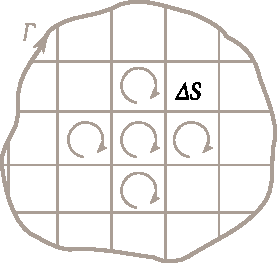
\includegraphics[scale=1]{figures/ch_01/fig_1_29.pdf}
		\caption[]{}
		\label{fig:1_29}
	\end{center}
	\vspace{-0.8cm}
\end{figure}

\textbf{Curl.} Tính cộng được của lưu số cho phép ta đưa ra khái niệm lưu số đơn vị, tức là, xét tỷ số giữa lưu số $C$ với độ lớn của bề mặt $S$ xung quanh nó lưu số ``chảy''. Với mặt $S$ hữu hạn, tỷ lệ $C/S$ cho giá trị trung bình của lưu số đơn vị. Giá trị này miêu tả đặc tính của trường trung bình trên mặt $S$. Để nhận được đặc trưng của trường tại điểm P, ta phải giảm kích thước bề mặt, làm nó co lại thành điểm P. Tỷ lệ $C/S$ tiến tới một giới hạn miêu tả đặc tính của trường tại điểm P.

Do đó, lấy một đường cong kín ảo $\Gamma$ trong một mặt phẳng đi qua điểm P, và xét biểu thức
\begin{equation}\label{eq:1_89}
	\lim_{S\to\text{P}} \frac{C_a}{S}
\end{equation}

\noindent
với $C_a$ là lưu số của vector $\vec{a}$ trên đoạn $\Gamma$ và $S$ là diện tích bề mặt giới hạn bởi đường cong kín.

Giới hạn \eqref{eq:1_89} được tính cho một mặt phẳng định hướng tùy ý không thể là một đặc tính toàn diện của trường tại P vì độ lớn của giới hạn này phụ thuộc vào hướng của đường cong kín trong không gian ngoài các đặc tính của trường tại điểm P. Hướng này có thể được cho bởi hướng của một pháp tuyến dương $\hatvec{n}$ đối với mặt phẳng đường cong kín (một pháp tuyến dương là cái mà liên kết với chiều di chuyển trên chu tuyến khi tích phân theo nguyên tắc nắm tay phải). Khi xác định giới hạn \eqref{eq:1_89} tại điểm P với hướng khác $\hatvec{n}$, ta sẽ nhận được giá trị khác. Với hướng ngược lại, giá trị này chỉ bị đổi dấu (sự đảo hướng $\hatvec{n}$ tương đương với sự đảo chiều di chuyển trên chu tuyến khi tích phân, cái mà chỉ làm đổi dấu lưu số ). Với một hướng xác định của pháp tuyến, độ lớn biểu thức \eqref{eq:1_89} tại điểm đã cho là cực đại.

Do đó, đại lượng \eqref{eq:1_89} như là hình chiếu của một vector lên hướng pháp tuyến của mặt phẳng chứa đường cong kín mà lưu số được lấy. Giá trị lớn nhất của đại lượng \eqref{eq:1_89} xác định độ lớn của vector này, và hướng của pháp tuyến dương $\hatvec{n}$ khi đạt giá trị lớn nhất là hướng của vector. Vector này gọi là \textbf{curl} của vector $\vec{a}$. Ký hiệu của nó là $\curl{\vec{a}}$. Sử dụng ký hiệu này, ta có thể viết biểu thức \eqref{eq:1_89} ở dạng
\begin{equation}\label{eq:1_90}
	(\curl{\vec{a}})_n = \lim_{S\to\text{P}} \frac{C_a}{S} = \lim_{S\to\text{P}} \frac{1}{S} \oint_S \vec{a}\, \deriv{\vec{l}}.
\end{equation}

Ta có thể nhận được hình ảnh minh họa về curl của vector $\vec{v}$ bằng cách tưởng tượng một cánh quạt nhỏ và nhẹ đặt tại điểm cho trước trong một chất lỏng đang chảy (\fig{1_30}). Tại những điểm mà curl khác không, cánh quạt sẽ quay, vận tốc nó càng lớn, khi giá trị hình chiếu của curl lên trục cánh quạt càng lớn.

Phương trình \eqref{eq:1_90} xác định vector $\curl{\vec{a}}$. Định nghĩa này là cái chung nhất mà không phụ thuộc vào loại hệ tọa độ sử dụng. Để tìm biểu thức cho hình chiếu của vector $\curl{\vec{a}}$ lên các trục tọa độ descartes, ta phải xác định giá trị của đại lượng \eqref{eq:1_90} theo hướng của diện tích $S$ mà pháp tuyến $\hatvec{n}$ của diện tích trùng với một trong các trục $x, y, z$. Giả sử, ta hướng $\hatvec{n}$ dọc theo trục $x$, từ đó \eqref{eq:1_90} trở thành $(\curl{\vec{a}})_x$.
Chu tuyến $\Gamma$ trong trường hợp này nằm trong mặt phẳng song song với mặt phẳng tọa độ $yz$. Ta lấy đường cong kín này ở dạng hình chữ nhật với cạnh $\Delta{y}$ và $\Delta{z}$ (\fig{1_31}, trục $x$ hướng về chúng ta trong hình này; chiều di chuyển biểu diễn trong hình liên kết với hướng của trục $x$ bởi định luật nắm tay phải). Đoạn $1$ của đường cong kín ngược hướng với trục $z$. Do đó, $a_l$ trên đoạn này là $-a_z$. Với lý do tương tự, $a$ trên đoạn $2$, $3$, và $4$ bằng $a_y$, $a_z$, và $-a_y$, tương ứng. Từ đó, lưu số có thể viết ở dạng
\begin{equation}\label{eq:1_91}
	\parenthesis{a_{z,3} - a_{z,1}} \Delta{z} - \parenthesis{a_{y,4} - a_{y,2}} \Delta{y}
\end{equation}

\noindent
Với $a_{z,3}$ và $a_{z,1}$ là giá trị trung bình của $a_z$ trên đoạn $3$ và $1$, tương ứng, $a_{y,4}$ và $a_{y,2}$ là giá trị trung bình của $a_{y}$ trên đoạn $4$ và $2$.

\begin{figure}[!htb]
	\begin{minipage}[t]{0.5\linewidth}
		\begin{center}
			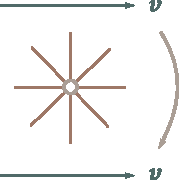
\includegraphics[scale=1]{figures/ch_01/fig_1_30.pdf}
			\caption[]{}
			\label{fig:1_30}
		\end{center}
	\end{minipage}
	\hspace{-0.1cm}
	\begin{minipage}[t]{0.5\linewidth}
		\begin{center}
			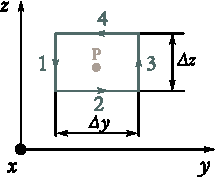
\includegraphics[scale=1]{figures/ch_01/fig_1_31.pdf}
			\caption[]{}
			\label{fig:1_31}
		\end{center}
	\end{minipage}
\vspace{-0.4cm}
\end{figure}

Hiệu $a_{z,3}-a_{z,1}$ là độ tăng giá trị trung bình của $a_z$ trên đoạn $\Delta{z}$ khi đoạn này dịch chuyển theo hướng của trục $y$ đoạn $\Delta{y}$. Nhờ độ nhỏ của $\Delta{y}$ và $\Delta{z}$, độ tăng này có thể biểu diễn ở dạng $(\diffinpartial{a_z}{y})\Delta{y}$, với giá trị của $\diffinpartial{a_z}{y}$ lấy tại điểm P\footnote{Sự thiếu chính xác ta chấp nhận ở đây biến mất khi đường bao co lại thành điểm P trong biến đổi giới hạn.}. Tương tự, hiệu $a_{y,4}-a_{y,2}$ có thể biểu diễn ở dạng $(\diffinpartial{a_y}{z})\Delta{z}$.
Sử dụng những biểu thức này trong \eqn{1_91} và đặt nhân tử chung ngoài dấu ngoặc đơn, ta nhận được biểu thức sau đây cho lưu số:
\begin{equation*}
	\parenthesis{\diffpartial{a_z}{y} - \diffpartial{a_y}{z}} \Delta{y}\Delta{z} = \parenthesis{\diffpartial{a_z}{y} - \diffpartial{a_y}{z}} \Delta{S}
\end{equation*}

\noindent
với $\Delta{S}$ là diện tích của đường cong kín. Chia lưu số cho $\Delta{S}$, ta được biểu thức cho hình chiếu của $\curl{\vec{a}}$ lên trục $x$:
\begin{equation}\label{eq:1_92}
	(\curl{\vec{a}})_x = \diffpartial{a_z}{y} - \diffpartial{a_y}{z}.
\end{equation}

\noindent
Bằng cách tương tự ta có thể tìm được
\begin{align}
	(\curl{\vec{a}})_y &= \diffpartial{a_x}{z} - \diffpartial{a_z}{x}, \label{eq:1_93}\\
	(\curl{\vec{a}})_z &= \diffpartial{a_y}{x} - \diffpartial{a_x}{y}. \label{eq:1_94}
\end{align}

Có thể dễ thấy rằng bất kỳ phương trình \eqref{eq:1_92}-\eqref{eq:1_94} có thể nhận được từ cái trước đó [\eqn{1_94} được xem như cái trước của \eqn{1_92}] bởi cái gọi là sự chuyển vị tuần hoàn của các tọa độ, tức là, thay thế các tọa độ theo cơ chế
\begin{equation*}
	\begin{tikzcd}[column sep=small]
x \arrow[rr, bend left] &           & y \arrow[ld, bend left] \\
                        & z \arrow[lu, bend left] &
\end{tikzcd}
\end{equation*}

Do đó, curl của vector $\vec{a}$ được xác định trong hệ tọa độ Descartes bởi biểu thức sau:
\begin{equation}\label{eq:1_95}
	\curl{\vec{a}} = \vecuni{x}\parenthesis{\diffpartial{a_z}{y} - \diffpartial{a_y}{z}} + \vecuni{y}\parenthesis{\diffpartial{a_x}{z} - \diffpartial{a_z}{x}} + \vecuni{z}\parenthesis{\diffpartial{a_y}{x} - \diffpartial{a_x}{y}}.
\end{equation}

\noindent
Dưới đây ta sẽ chỉ ra một cách tinh tế hơn để viết biểu thức này.

\textbf{Định lý Stokes.} Biết curl của vector $\vec{a}$ tại mọi điểm trên mặt $S$ (không nhất thiết là mặt phẳng), ta có thể tính lưu số của vector này trên chu tuyến $\Gamma$ giới hạn $S$ (chu tuyến cũng có thể không nằm trong một mặt phẳng). Vì ý định này, ta chia bề mặt thành các phần tử rất nhỏ $\Delta{S}$. Do độ nhỏ của chúng, những phần tử này có thể xem như mặt phẳng. Do đó theo \eqn{1_90}, lưu số của vector $\vec{a}$ trên đường cong kín giới hạn $\Delta{S}$ có thể viết ở dạng
\begin{equation}\label{eq:1_96}
	\Delta{C} \approx (\curl{\vec{a}})_n \Delta{S} = \curl{\vec{a}} \ccdot \Delta{\vec{S}}
\end{equation}

\noindent
Với $\hatvec{n}$ là một pháp tuyến dương của phần tử bề mặt $\Delta{S}$.

Theo \eqn{1_88}, tổng của biểu thức \eqref{eq:1_96} trên tất cả $\Delta{S}$ dẫn đến lưu số của vector $\vec{a}$ trên đường cong kín $\Gamma$ giới hạn $S$:
\begin{equation*}
	C = \sum\Delta{C} \approx \sum\curl{\vec{a}} \ccdot \Delta{\vec{S}}.
\end{equation*}

\noindent
Thực hiện biến đổi giới hạn tất cả $\Delta{S}$ tiến tới không (số lượng của chúng tăng không giới hạn), ta được phương trình
\begin{equation}\label{eq:1_97}
	\oint_{\Gamma} \vec{a}\ccdot\deriv{\vec{l}} = \int_S (\curl{\vec{a}}) \ccdot \Delta{\vec{S}}.
\end{equation}

\noindent
Phương trình \eqref{eq:1_97} gọi là \textbf{Định lý Stokes}. Ý nghĩa của nó là lưu số của vector $\vec{a}$ trên một đường cong kín tùy ý $\Gamma$ bằng thông lượng của vector $\curl{\vec{a}}$ qua bề mặt tùy ý $S$ giới hạn bởi đường cong kín cho trước.

\textbf{Toán tử Del}. Viết công thức phân tích vector được đơn giản hóa đáng kể nếu ta đưa vào một toán tử vi phân ký hiệu bởi biểu tượng $\nabla$ (nabla hoặc del) và gọi là \textbf{toán tử del} hoặc \textbf{toán tử Hamilton}. Toán tử này biểu diễn một vector với các thành phần $\diffinpartial{}{x}$, $\diffinpartial{}{y}$ và $\diffinpartial{}{z}$. Kết quả là,
\vspace{-10pt}
\begin{equation}\label{eq:1_98}
	\nabla = \vecuni{x}\diffpartial{}{x} + \vecuni{y}\diffpartial{}{y} + \vecuni{z}\diffpartial{}{z}.
\end{equation}

\noindent
Vector này tự nó không có nghĩa. Nó có nghĩa khi kết hợp với hàm vô hướng hoặc hàm vector mà nó được nhân một cách tượng trưng. Do đó, nếu ta nhân vector $\nabla$ với hàm vô hướng $\varphi$ ta được vector
\begin{equation}\label{eq:1_99}
	\gradop{\varphi} = \vecuni{x}\diffpartial{\varphi}{x} + \vecuni{y}\diffpartial{\varphi}{y} + \vecuni{z}\diffpartial{\varphi}{z}
\end{equation}

\noindent
Là gradient của hàm $\varphi$ [xem \eqn{1_68}].

Tích vô hướng của vector $\nabla$ và $\vec{a}$ cho ta hàm vô hướng
\begin{equation}\label{eq:1_100}
	\divop{\vec{a}} = \nabla_{x}a_{x} + \nabla_{y}a_{y} + \nabla_{z}a_{z}
\end{equation}

\noindent
mà ta có thể xem như divergence của vector $\vec{a}$ [xem \eqn{1_81}].

Cuối cùng, tích vector của vector $\nabla$ và $\vec{a}$ cho ta một vector với các thành phần $(\curlop{\vec{a}})_x=\nabla_{y}a_{z} - \nabla_{z}a_{y}=\diffinpartial{a_z}{y}-\diffinpartial{a_y}{z}$, vân vân., trùng với các thành phần của $\curl{\vec{a}}$ [xem Phương trình. \eqref{eq:1_92}-\eqref{eq:1_94}]. Từ đó, sử dụng cách viết tích vector bằng định thức, ta có
\begin{equation}\label{1_101}
	\curl{\vec{a}} = \curlop{\vec{a}} = \begin{vmatrix}
	\vecuni{x} & \vecuni{y} & \vecuni{z}\\
	\diffpartial{}{x} & \diffpartial{}{y} & \diffpartial{}{z}\\
	a_x & a_y & a_z
	\end{vmatrix}.
\end{equation}

Do đó, có hai cách biểu diễn gradient, divergence, và curl:
\begin{equation*}
	\gradop{\varphi}\equiv\grad{\varphi},\quad \divop{\vec{a}}\equiv\diverg{\vec{a}},\quad \curlop{\vec{a}}\equiv\curl{\vec{a}}.
\end{equation*}

\noindent
Việc sử dụng ký hiệu del có một số ưu điểm. Do đó ta sẽ sử dụng ký hiệu này trong phần sau. Người ta đã quen nhận định ký hiệu $\gradop{\varphi}$ là ``gradient của phi'' (tức là, không nói ``del phi'', mà là ``gradient of phi''), ký hiệu $\divop{\vec{a}}$ là ``divergence của a'' và, cuối cùng, ký hiệu $\curlop{\vec{a}}$ là ``curl của a''.

Khi sử dụng vector $\nabla$, phải nhớ rằng nó là toán tử vi phân tác dụng lên tất cả hàm ở bên phải của nó. kết quả là, trong các biểu thức biến đổi chứa $\nabla$, ta phải xem xét cả hai quy tắc của đại số vector và giải tích vi phân. Ví dụ, đạo hàm của tích hàm số $\varphi$ và $\psi$ là
\begin{equation*}
	(\varphi\psi)' = \varphi'\psi + \varphi\psi'.
\end{equation*}

\noindent
Do đó,
\begin{equation}\label{eq:1_102}
	\grad{(\varphi\psi)} = \gradop{(\varphi\psi)} = \psi\gradop{\varphi} + \varphi\gradop{\psi} = \psi\,\grad{\varphi} + \varphi\,\grad{\psi}.
\end{equation}

\noindent
Tương tự,
\begin{equation}\label{eq:1_103}
	\diverg{(\varphi\vec{a})} = \divop{(\varphi\vec{a})} = \vec{a}\ccdot(\gradop{\varphi}) + \varphi(\divop{\vec{a}}).
\end{equation}

Gradient của hàm $\varphi$ là một hàm vector. Do đó, divergence và curl có thể áp dụng lên nó:
\begin{align}
	\diverg{\grad{\varphi}} &= \divop{\gradop{\varphi}} = (\divop{\nabla})\varphi = \parenthesis{\nabla_x^2 + \nabla_y^2 + \nabla_z^2}\varphi\nonumber\\
	&= \diffsecpartial{\varphi}{x} + \diffsecpartial{\varphi}{y} + \diffsecpartial{\varphi}{z} = \upDelta{\varphi}\label{eq:1_104}
\end{align}

\noindent
($\upDelta$ là toán tử Laplace)
\begin{equation}\label{eq:1_105}
	\curl{\grad{\varphi}} = \curlop{(\gradop{\varphi})} = (\curlop{\nabla})\varphi
\end{equation}

\noindent
(nhớ rằng tích vector của một vector với chính nó là không).

Ta hãy áp dụng divergence và curl lên hàm $\curl{\vec{a}}$:
\begin{equation}\label{eq:1_106}
	\diverg{\curl{\vec{a}}} = \divop{\curlop{\vec{a}}} = 0
\end{equation}

\noindent
(một tích vô hướng bội ba bằng với thể tích của một hình hộp được xây dựng trên các vector được nhân (xem Tập I, phần 22); nếu có hai vector trong số đó trùng nhau, thể tích của hình hộp bằng không):
\begin{equation}\label{eq:1_107}
	\curl{\curl{\vec{a}}} = \curlop{(\curlop{\vec{a}})} = \gradop{(\divop{\vec{a}})} - (\divop{\nabla})\vec{a} = \grad{\diverg{\vec{a}}} - \upDelta{\vec{a}}
\end{equation}

\noindent
[ta đã sử dụng phương trình (1.35) của tập I, cụ thể là, $\vec{a}\times\vec{b}\times\vec{c} = \vec{b}(\vecdot{a}{c}) - \vec{c}(\vecdot{a}{b})$].

Phương trình \eqref{eq:1_106} chỉ ra rằng trường của curl không có nguồn. Từ đó, các đường sức của vector $\curl{\vec{a}}$ không có điểm bắt đầu cũng như kết thúc. Chính vì lý do này mà thông lượng của curl qua bất kì bề mặt $S$ tựa lên đường cong kín cho trước $\Gamma$ là như nhau [xem \eqn{1_97}).

Ta sẽ lưu ý ở kết luận khi toán tử del được sử dụng, Phương trình \eqref{eq:1_82} và \eqref{eq:1_97} có thể ở dạng
\begin{align}
	\oint_S \vec{a} \ccdot \deriv{\vec{S}} &= \oint_V \divop{\vec{a}}\, \deriv{V},\quad\quad\! \text{(Định lý Ostrogradsky-Gauss)}\label{eq:1_108}\\
	\oint_{\Gamma} \vec{a} \ccdot \deriv{\vec{l}} &= \int_S (\curlop{\vec{a}}) \ccdot \deriv{\vec{S}}.\quad \text{(Định lý Stokes)}\label{eq:1_109}
\end{align}

\section{Lưu Số và Curl của Trường Tĩnh Điện}\label{sec:1_12}

Chúng ta đã thành lập ở \sect{1_6} rằng lực tác dụng lên điện tích $q$ trong trường tĩnh điện có tính bảo toàn. Vì thế, công mà lực này thực hiện trên một đường cong kín $\Gamma$ bằng không:
\begin{equation*}
	A = \oint_{\Gamma} q\vec{E} \ccdot \deriv{\vec{l}} = 0.
\end{equation*}

\noindent
Triệt tiêu $q$, chúng ta có
\begin{equation}\label{eq:1_110}
	\oint_{\Gamma} \vec{E} \ccdot \deriv{\vec{l}} = 0
\end{equation}

\noindent
(so sánh với \eqn{1_46}]

Tích phân ở vế trái của \eqn{1_110} là lưu số vector điện trường $\vec{E}$ trên toàn chu tuyến $\Gamma$ [xem phép khai triển \eqref{eq:1_80}]. Do đó, \textit{một trường tĩnh điện luôn có lưu số vector điện trường của một đường cong kín bất kì bằng không}.

Chọn một mặt $S$ nằm trên chu tuyến $\Gamma$, với lưu số điện trường đã biết (\fig{1_32}). Theo định lý Stokes [xem \eqn{1_109}], tích phân của $\curl{\vec{E}}$ trên toàn bộ bề mặt bằng với lưu số vector điện trường $\vec{E}$ trên toàn chu tuyến $\Gamma$:
\begin{equation}\label{eq:1_111}
	\int_S (\curlop{\vec{E}}) \ccdot \deriv{\vec{S}} = \oint_{\Gamma} \vec{E} \ccdot \deriv{\vec{l}}.
\end{equation}

\noindent
Mặt khác lưu số bằng không, nên ta sẽ có
\begin{equation*}
	\int_S (\curlop{\vec{E}}) \ccdot \deriv{\vec{S}} = 0.
\end{equation*}

\noindent
Điều kiện này là luôn đúng với mọi mặt $S$ nằm trên chu tuyến $\Gamma$ bất kì. Miễn là curl của vector $\vec{E}$ tại một điểm bất kì trong không gian bằng không:

\begin{equation}\label{eq:1_112}
	\curlop{\vec{E}} = 0.
\end{equation}

\begin{figure}[!htb]
	\begin{minipage}[t]{0.5\linewidth}
		\begin{center}
			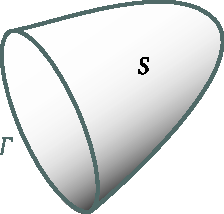
\includegraphics[scale=0.95]{figures/ch_01/fig_1_32.pdf}
			\caption[]{}
			\label{fig:1_32}
		\end{center}
	\end{minipage}
	\hspace{-0.1cm}
	\begin{minipage}[t]{0.5\linewidth}
		\begin{center}
			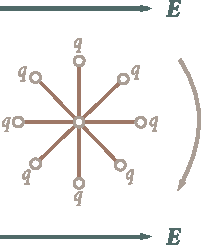
\includegraphics[scale=0.95]{figures/ch_01/fig_1_33.pdf}
			\caption[]{}
			\label{fig:1_33}
		\end{center}
	\end{minipage}
\vspace{-0.4cm}
\end{figure}

Ta xét mô hình quạt ở \fig{1_25}, với mỗi đầu của nó được đính những điện tích dương $q$ (\fig{1_33}; toàn bộ hệ này phải có kích thước rất nhỏ). Nếu tại một điểm bất kì trong điện trường mà $\curl{\vec{E}}$ khác không, mô hình ta đề cập ở trên sẽ quay với một gia tốc tỉ lệ thuận với hình chiếu của curl lên trục quay. Nhưng, với trường tĩnh điện, những mô hình như trên sẽ không quay theo bất kì hướng nào.

Như thế, đặc điểm của trường tĩnh điện là nó không phải là trường xoáy. Chúng ta đã chứng tỏ được điều này vì curl của gradient của một hàm vô hướng luôn bằng không [xem biến đổi ở \eqref{eq:1_96}]. Vì thế, việc $\curl{\vec{E}}$ bằng không tại mọi điểm trong không gian giúp ta viết được biểu thức của $\vec{E}$ dưới dạng gradient của hàm vô hướng (mà ta đã biết nó là điện thế). Chúng ta đã xem xét biểu thức này ở \sect{1_8} [xem \eqn{1_41}; dấu trừ của biểu thức này được suy ra từ các lập luận vật lý]. 

Theo điều kiện từ \eqref{eq:1_110}, thì ta sẽ lập tức nhận ra rằng trường tĩnh điện ở \fig{1_34} là bất khả thi. Với một trường như hình trên, thì lưu số quanh một chu tuyến, mô tả bởi đường nét đứt, thì khác không. Điều này sẽ mâu thuẫn với điều kiện \eqref{eq:1_110}. Nó cũng bất khả thi với việc tồn tại một điện trường đều (khác không) bên trong một thể tích xác định (\fig{1_35}). Trong trường hợp này chu tuyến mô tả bởi đường nét đứt sẽ có lưu số khác không.

\begin{figure}[!htb]
	\begin{minipage}[t]{0.36\linewidth}
		\begin{center}
			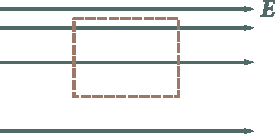
\includegraphics[scale=0.93]{figures/ch_01/fig_1_34.pdf}
			\caption[]{}
			\label{fig:1_34}
		\end{center}
	\end{minipage}
	% \hspace{-0.05cm}
	\hfill{ }
	\begin{minipage}[t]{0.2\linewidth}
		\begin{center}
			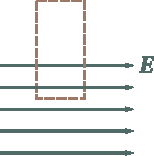
\includegraphics[scale=0.93]{figures/ch_01/fig_1_35.pdf}
			\caption[]{}
			\label{fig:1_35}
		\end{center}
	\end{minipage}
	% \hspace{-0.05cm}
	\hfill{ }
	\begin{minipage}[t]{0.37\linewidth}
		\begin{center}
			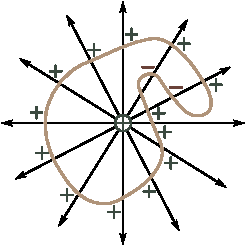
\includegraphics[scale=0.95]{figures/ch_01/fig_1_36.pdf}
			\caption[]{}
			\label{fig:1_36}
		\end{center}
	\end{minipage}
\vspace{-0.45cm}
\end{figure}

\section{Định Luật Gauss}\label{sec:1_13}

Chúng ta đã tính được curl trong một trường tĩnh điện ở chương trước. Giờ chúng ta sẽ đi tìm divergence của nó. Để bắt đầu, chúng ta thử xét trường của một điện tích điểm $q$ và tính thông lượng vector $\vec{E}$ qua diện tích mặt kín $S$ bao lấy điện tích (\fig{1_36}). Chúng ta đã biết được từ \sect{1_5} rằng tổng số đường sức vector $\vec{E}$ phân kỳ từ $q$ hay hội tụ tại $-q$ đều có giá trị đại số là $q/\varepsilon_0$.

Từ \eqn{1_77} ta biết rằng thông lượng của vector $\vec{E}$ qua một diện tích mặt kín bằng với số đường sức thoát ra (nếu điện tích dương), hoặc số đường sức đâm vào (nếu điện tích âm). Cho rằng số đường sức thoát ra hay đâm vào đều có giá trị đại số bằng $q/\varepsilon_0$ (xem \sect{1_5}), chúng ta có thể viết được
\begin{equation}\label{eq:1_113}
	\Phi_E = \frac{q}{\varepsilon_0}.
\end{equation}

\noindent
Dấu của thông lượng phụ thuộc vào dấu của $q$. Thứ nguyên của hai vế là giống nhau.

Giờ chúng ta xét một mặt kín chứa $N$ điện tích $q_1, q_2, \ldots, q_N$. Theo nguyên lý chồng chất, cường độ $\vec{E}$ của hệ sẽ là tổng hợp các cường độ $\vec{E_i}$ của từng điện tích: $\vec{E}=\sum_i\vec{E}_i$
\begin{equation*}
	\Phi_E = \oint_S \vec{E}\ccdot\deriv{\vec{S}} = \oint_S \parenthesis{\sum_i\vec{E}_i}\ccdot\deriv{\vec{S}} = \sum_i\oint_S\vec{E}_i\ccdot\deriv{\vec{S}}.
\end{equation*}

\noindent
Mỗi tích phân bên trong dấu sum bằng $q_i/\varepsilon_0$. Vì thế,
\begin{equation}\label{eq:1_114}
	\Phi_E = \oint_S \vec{E}\ccdot\deriv{\vec{S}} = \frac{1}{\varepsilon_0} \sum_{i=1}^N q_i.
\end{equation}

\noindent
Biểu thức chúng ta vừa tìm được được gọi là \textbf{định luật Gauss}. Dựa theo định lý, \textit{thông lượng của vector điện trường qua diện tích mặt kín bằng với tổng đại số điện tích được chứa trong mặt kín chia cho $\varepsilon_0$}.

Khi xem xét trường tạo ra bởi một hệ điện tích vĩ mô (là hệ được cấu tạo từ vô số các điện tích nguyên tố), ta bỏ qua sự rời rạc trong cấu trúc, và cho rằng nó được phân bố trong không gian liên tục với một mật độ xác định tại mọi nơi. \textbf{Mật độ điện tích khối của một điện tích} $\rho$ được xác định tương tự với khối lượng riêng. Chỉ khác là, ta lấy tỉ lệ giữa $\deriv{q}$ trên một thể tích nhỏ vô hạn (theo quan điểm vật lý) $\deriv{V}$ mà chứa điện tích trên:
\begin{equation}\label{eq:1_115}
	\rho = \diff{q}{V}.
\end{equation}

\noindent
Khi nói về một thể tích rất nhỏ, chúng ta phải hiểu rằng đó là thể tích chứa một lượng điện tích xác định và phân bố đều trong thể tích ấy. Tuy nhiên, vùng thể tích này phải rất lớn so với thể tích của một điện tích nguyên tố riêng lẻ.

Biết được mật độ điện khối trong không gian, chúng ta có thể tính được tổng điện tích được giữ bên trong bề mặt kín $S$. Để tính được điện tích, ta cần phải lấy tích phân của $\rho$ trên toàn bộ thể tích bị giới hạn bởi mặt kín $S$.
\begin{equation*}
	\sum_i q_i = \int_V \rho\,\deriv{V}.
\end{equation*}

\noindent
Ngoài ra, \eqn{1_114} có thể được viết là
\begin{equation}\label{eq:1_116}
	\oint_S \vec{E}\ccdot\deriv{\vec{S}} = \frac{1}{\varepsilon_0} \int_V \rho\,\deriv{V}.
\end{equation}

Theo tích phân Gauss (\eqn{1_108}), chúng ta sẽ có
\begin{equation*}
	\int_V \divop{\vec{E}}\,\deriv{V} = \frac{1}{\varepsilon_0} \int_V \rho\,\deriv{V}.
\end{equation*}

\noindent
Phương trình mà chúng ta vừa thành lập có thể sử dụng cho mọi miền thể tích $V$. Điều này có nghĩa là các biểu thức bên trong dấu tích phân phải bằng nhau tại mọi điểm trong không gian. Từ đây, ta thấy rằng liên hệ giữa divergence của vector $\vec{E}$ và mật độ điện khối là

\begin{equation}\label{eq:1_117}
	\divop{\vec{E}} = \frac{1}{\varepsilon_0} \rho.
\end{equation}

\noindent
Phương trình này còn được gọi là dạng vi phân của định lý Gauss.

Khi xét một dòng chảy chất lỏng, $\divop{\vec{v}}$ cho biết công suất được thực hiện bởi nguồn tại một điểm xác định. Tương tự, đối với tĩnh điện thì điện tích được coi tương tự như nguồn nước ở trường hợp trên. 

\section{Một Số Vận Dụng Của Định Luật Gauss }\label{sec:1_14}

Định luật Gauss cho phép chúng ta tính toán cường độ điện trường một cách đơn giản hơn việc sử dụng $\eqn{1_15}$ để tổng hợp cường độ điện trường của từng điện tích điểm. Một số ví dụ sau đây sẽ có thể cho ta thấy được sự tiện lợi của định luật Gauss. Điều này sẽ giúp chúng ta rất nhiều trong nghiên cứu sâu hơn về điện trường. Trước khi bắt đầu, chúng ta nên tiếp cận đến khái niệm mật độ điện mặt và mật độ điện dài.

Nếu một vật có điện tích được phân bố đều trên bề mặt của nó, thì sự phân bố đó sẽ được đặc trưng bằng đại lượng $\sigma$, hay còn được biết đến là mật độ điện mặt, được xác định bằng
\begin{equation}\label{eq:1_118}
	\sigma = \diff{q}{S}.
\end{equation}

\noindent
Ở đây $\deriv{q}$ là điện tích nằm trong phần diện tích $\deriv{S}$. Với $\deriv{S}$ là diện tích vi phân.

Nếu điện tích được phân bố dọc theo độ dài của một ống trụ (Xét mặt cắt vuông góc với trục ống, mật độ điện mặt của nó là không đổi trên toàn mặt đó), chúng ta sẽ sử dụng đại lương gọi là \textit{mật độ điện dài}
\begin{equation}\label{eq:1_119}
	\lambda = \diff{q}{l}
\end{equation}

\noindent
Ở đây, $\deriv{l}$ là độ dài vi phân dọc theo độ dài dây, và $\deriv{q}$ là điện tích chứa trong ống trụ vi phân trên.

\textbf{Điện trường của Mặt Phẳng Vô Hạn phân bố đều.} Ta giả sử rằng mật độ điện mặt tại mọi điểm là xác định và đều bằng $\sigma$; để tổng quát hoá biểu thức, ta cho rằng điện tích là dương. Do tính đối xứng của sự vô hạn, điện trường sẽ có hướng vuông góc với mặt phẳng. Bởi vì, do tấm rộng vô hạn và phân bố điện tích đều, nên không lý do gì để vector $\vec{E}$ bị nghiêng so với phương vuông góc mặt phẳng. Hai miền đối diện nhau được chia cắt bởi bờ là mặt phẳng vô hạn, cường độ điện trường của chúng cùng độ lớn và ngược chiều nhau.

\begin{figure}[!htb]
	\begin{minipage}[t]{0.5\linewidth}
		\begin{center}
			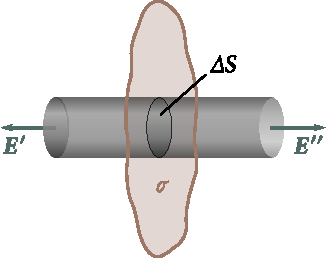
\includegraphics[scale=1]{figures/ch_01/fig_1_37.pdf}
			\caption[]{}
			\label{fig:1_37}
		\end{center}
	\end{minipage}
	\hspace{-0.05cm}
	\begin{minipage}[t]{0.5\linewidth}
		\begin{center}
			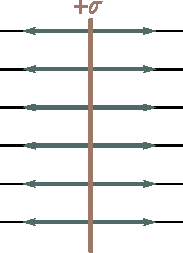
\includegraphics[scale=1]{figures/ch_01/fig_1_38.pdf}
			\caption[]{}
			\label{fig:1_38}
		\end{center}
	\end{minipage}
\vspace{-0.4cm}
\end{figure}

Giờ chúng ta giả sử có một ống trụ, trục của nó vuông góc với mặt phẳng, đáy có diện tích bằng $\Delta{S}$, ống trụ đối xứng hai bên (trung điểm thuộc bề mặt tích điện). Bởi vì đối xứng, chúng ta có $E'=E''=E$. Ta áp dụng định luật Gauss cho các mặt này. Thông lượng qua diện tích mặt bên của ống trụ bằng không, vì $E_n$\footnote{$E_n$ là vector điện trường vuông góc với bề mặt đang xét} tại mỗi điểm đều vuông góc với mặt trụ bên. Tại ngay trên bề mặt, $E_n$ trùng với $E$. Tổng thông lượng qua mặt là $2E\Delta{S}$. Điện tích của mặt phẳng được chứa trong mặt trụ là $\sigma\Delta{S}$. Theo định luật Gauss, ta sẽ có
\begin{equation*}
	2E\Delta{S} = \frac{\sigma\Delta{S}}{\varepsilon_0}
\end{equation*}

\noindent
suy ra
\begin{equation}\label{eq:1_120}
	E = \frac{\sigma}{2\varepsilon_0}.
\end{equation}

\noindent
Kết quả mà chúng ta nhận được không phụ thuộc vào chiều dài của ống trụ mà ta xét. Điều này cho ta thấy rằng cường độ điện trường có độ lớn không phụ thuộc vào khoảng cách đến mặt. Đường sức được mô tả ở \fig{1_38}. Nếu với trường hợp điện tích âm, kết quả vẫn như vậy, chỉ khác là vector $\vec{E}$ và đường sức bị đảo chiều.

Nếu mặt phẳng mà chúng ta xét không phải vô hạn, ví dụ như một đĩa mỏng bị tích điện\footnote{Đối với một đĩa, $\sigma$ ở \eqn{1_120} nên được hiểu là điện tích chứa trong \SI{1}{\metre\squared} nhân độ dày của nó. Với vật dẫn kim loại, điện tích được phân bố trên mặt ngoài của nó. Nên nếu ta xét một mặt của nó thì ta có $\sigma$ chỉ bằng một nửa khi xét toàn đĩa.}, thì kết quả trên chỉ còn đúng cho những điểm mà khoảng cách của nó tới rìa mặt phẳng rất lớn so với khoảng cách của nó đến bề mặt tích điện (trong \fig{1_39} vùng dưới đường nét đứt là vùng chúng ta đang nói tới). Khi xét một điểm càng xa bản tụ hoặc đến gần rìa của nó, thì nó không còn được coi là mặt phẳng vô hạn nữa. Dễ thấy rằng, khi đặt mặt phẳng vào một không gian rộng, thì điện trường mà nó gây ra giống như một điện tích điểm.

\textbf{Điện Trường của Hai Mặt Phẳng Tích Điện Đều.} Điện trường gây ra bởi hai mặt phẳng rộng vô hạn với độ lớn mật độ điện mặt không đổi $\sigma$ có thể tính được dựa vào tổng hợp điện trường của từng mặt (\fig{1_40}). Ở khoảng không gian giữa hai mặt phẳng, điện trường được tổng hợp cùng hướng, nên nó có giá trị là
\begin{equation}\label{eq:1_121}
	E = \frac{\sigma}{\varepsilon_0}.
\end{equation}

\noindent
Ở vùng không gian bên ngoài hai mặt phẳng thì điện trường triệt tiêu nhau nên nó có giá trị bằng không tại mọi điểm.

\begin{figure}[!htb]
	\begin{minipage}[t]{0.5\linewidth}
		\begin{center}
			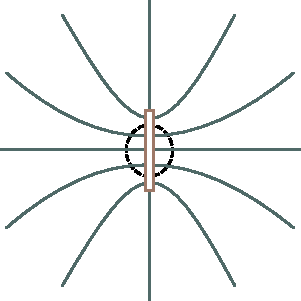
\includegraphics[scale=1]{figures/ch_01/fig_1_39.pdf}
			\caption[]{}
			\label{fig:1_39}
		\end{center}
	\end{minipage}
	\hspace{-0.05cm}
	\begin{minipage}[t]{0.5\linewidth}
		\begin{center}
			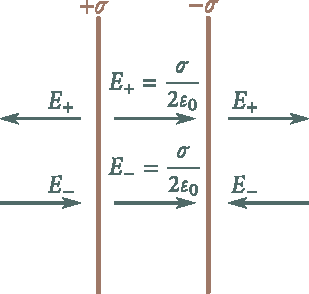
\includegraphics[scale=1]{figures/ch_01/fig_1_40.pdf}
			\caption[]{}
			\label{fig:1_40}
		\end{center}
	\end{minipage}
\vspace{-0.55cm}
\end{figure}

Vì thế, điện trường chỉ tồn tại ở giữa hai mặt phẳng tích điện. Điện trường này có giá trị không đổi và chỉ hướng về một phía; vì thế, nó là điện trường đều. Đường sức điện là những đường thẳng song song cách đều nhau.

Kết quả mà chúng ta nhận được cũng đúng cho trường hợp mặt phẳng không vô hạn, nhưng khoảng cách giữa chúng là vô cùng bé so với độ rộng của chúng (nó còn được gọi là tụ điện phẳng). Trong trường hợp này, tại rìa của chúng, có xuất hiện những sai lệch so với các tính toán trên của ta (như \fig{1_41}).

\textbf{Điện Trường của Mặt Trụ Tích Điện.} Cho rằng ống trụ (bán kính R) có mật độ điện mặt không đổi là $\sigma$. Vì tính đối xứng, nên điện trường gây ra bởi ống trụ có phương xuyên tâm, và giá trị của nó chỉ phụ thuộc vào khoảng cách $r$ đến trục ống trụ. Chúng ta vẽ ra một mặt trụ đồng trục có bán kính $r$ và độ cao là $h$. Với mặt đáy của hình trụ, chúng ta có $E_n=0$ (Ta giả sử điện tích là dương). Vì thế ta có thế tính điện thông của vector $\vec{E}$ qua mặt này bằng $E(r)\times 2\pi rh$. Nếu $r>R$, điện tích là $q=\lambda h$ (với $\lambda$ là mật độ điện dài) được chứa trong mặt trụ. Áp dụng định lý Gauss, ta có thể tìm được 
\begin{equation*}
	E(r)\times 2\pi rh = \frac{2\lambda}{\varepsilon_0}.
\end{equation*}

\noindent
Do đó,
\begin{equation}\label{eq:1_122}
	E(r) = \frac{1}{2\pi\varepsilon_0}\frac{\lambda}{r}\quad (r\geqslant R).
\end{equation}

\noindent
Nếu $r<R$, không có điện tích nào được chứa bên trong mặt trụ, vì thế $E(r)=0$.

\begin{figure}[!htb]
	\begin{minipage}[t]{0.35\linewidth}
		\begin{center}
			
\includegraphics[scale=1]{figures/ch_01/fig_1_41.pdf}
			\caption[]{}
			\label{fig:1_41}
		\end{center}
	\end{minipage}
	\hspace{-0.05cm}
	\begin{minipage}[t]{0.65\linewidth}
		\begin{center}
			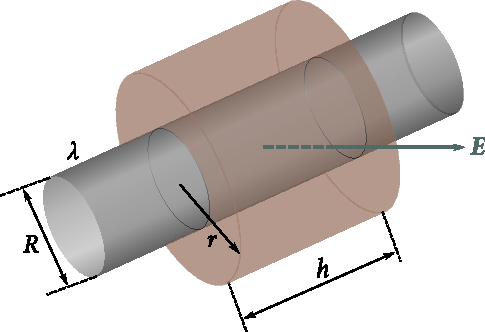
\includegraphics[scale=0.95]{figures/ch_01/fig_1_42.pdf}
			\caption[]{}
			\label{fig:1_42}
		\end{center}
	\end{minipage}
\vspace{-0.4cm}
\end{figure}

Cũng từ đó ta thấy được rằng, nó không tồn tại điện trường bên trong một ống trụ tích điện đều dài vô hạn. Điện trường ở không gian bên ngoài thì phụ thuộc vào mật độ điện tích dài $\lambda$ và khoảng cách tới trục $r$.

Đối với ống trụ tích điện âm, thì chỉ khác ở chiều của điện trường $\vec{E}$ bên ngoài ống. Theo \eqn{1_112}, khi ta càng tiến gần về phía bề mặt của ống trụ (với mật độ $\lambda$ không đổi), thì điện trường có giá trị càng lớn. Và nó đạt giá trị lớn nhất tại ngay mặt của ống trụ. 

Ta có $\lambda=2\pi R\sigma$, thế nó vào $\eqn{1_122}$ và xét tại $r=R$, chúng ta sẽ nhận được điện trường tại gần bề mặt trụ là: 
\begin{equation}\label{eq:1_123}
	E(R) = \frac{\sigma}{\varepsilon_0}.
\end{equation}

Chúng ta có thể tính được điện trường do hai ống trụ đồng trục (tích mật độ như nhau nhưng trái dấu) tạo ra bằng nguyên lý chồng chất ($\fig{1_43}$). Ta nhận thấy rằng, không có điện trường bên trong ống trụ nhỏ hay bên ngoài ống trụ lớn. Điện trường ở vùng không gian giữa hai mặt được xác định thông qua $\eqn{1_122}$. Điều này cũng đúng cho ống trụ hữu hạn nhưng khoảng cách giữa hai mặt là rất bé (được gọi là tụ trụ). Khi lại gần rìa của ống trụ, thì điện trường tại đó sẽ bị sai lệch so với những tính toán ta đã làm trên.

\begin{figure}[!htb]
	\begin{center}
		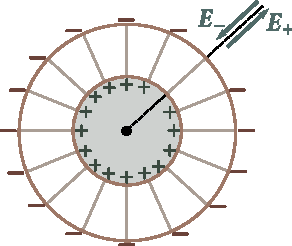
\includegraphics[scale=1]{figures/ch_01/fig_1_43.pdf}
		\caption[]{}
		\label{fig:1_43}
	\end{center}
	\vspace{-0.8cm}
\end{figure}

\textbf{Điện trường của Mặt Cầu Tích Điện.} Điện trường tạo ra bởi một mặt cầu có bán kính $R$ được tích điện với mật độ đều $\sigma$ là đối xứng qua tâm. Điều này có nghĩa là phương của vector $\vec{E}$ sẽ đi qua tâm của hình cầu, với độ lớn của $\vec{E}$ là một hàm của $r$ tính từ tâm. Ta dựng một măt cầu đồng tâm với quả cầu trên. Với mọi điểm trên bề mặt này, thì $E_n=E(r)$. Nếu $r>R$, thì toàn bộ điện tích trên quả cầu đều nằm trong mặt cầu. Vì thế,
\begin{equation*}
	E(r)\times 4\pi r^2 = \frac{q}{\varepsilon_0}
\end{equation*}

\noindent
whence hay
\begin{equation}\label{eq:1_124}
	E(r) = \frac{1}{4\pi\varepsilon_0}\frac{q}{r^2}.\quad (r\geqslant R)
\end{equation}

Với mặt cầu có bán kính $r$ bé hơn $R$ nó sẽ không chứa điện tích, vì thế với $r<R$ thì chúng ta có $E(r)=0$.

Do đó, không có điện trường ở bên trong quả cầu tích điện với mật độ mặt đều $\sigma$. Bên ngoài quả cầu, điện trường sẽ tương tự như một điện tích điểm, có giá trị bằng tổng điện tích của quả cầu và đặt tại tâm.

Theo nguyên lý chồng chất điện trường, chúng ta có thể dễ dàng tính điện trường giữa hai mặt cầu đồng tâm (còn được gọi là tụ cầu) mang lần lượt điện tích $+q$ và $-q$ có cùng giá trị xác định. Điện trường có thể được tính thông qua \eqn{1_124}.

\textbf{Điện Trường của Quả Cầu Điện Tích.} Cho một quả cầu bán kính $R$ có điện tích phân bố đều bên trong quả cầu với một mật độ $\rho$. Điện trường trong trường hợp là đối xứng xuyên tâm. Ta dễ dàng thấy rằng, điện trường bên ngoài của nó giống như ở trường hợp mặt cầu tích điện ta xét vừa rồi [xem \eqn{1_124}]. Nhưng kết quả sẽ khác nhau khi xét bên trong lòng quả cầu. Lấy một mặt cầu bán kính $r$ (với $r<R$), điện trường chứa bên trong nó là $\rho\times 4\pi r^3/3$. Thế nên, định luật Gauss cho mặt này ta được:
\begin{equation*}
	E(r)\times 4\pi r^2 = \frac{1}{\varepsilon_0}\rho \frac{4}{3}\pi r^3.
\end{equation*}

\noindent
Ta thay $q/(4\pi R^3/3)$ bằng $\rho$, ta sẽ có
\begin{equation}\label{eq:1_125}
	E(r) = \frac{1}{4\pi\varepsilon_0}\frac{q}{R^3}r.\quad (r\leqslant R)
\end{equation}

Từ đấy, ta thấy rằng điện trường bên trong quả cầu có dạng tuyến tính phụ thuộc theo $r$ (tính từ tâm). Bên ngoài quả cầu, điện trường tương tự với một điện tích đặt ở tâm quả cầu.

\cleardoublepage
%% !TEX root = saveliev_physics_general_course_2.tex
%!TEX TS-program = pdflatex
%!TEX encoding = UTF-8 Unicode


\chapter{ĐIỆN TRƯỜNG TRONG ĐIỆN MÔI}\label{chap:2}

\section{Phân tử phân cực và không phân cực}\label{sec:2_1}

Điện môi (hoặc vật cách điện) được định nghĩa là chất không có khả năng dẫn điện. Vật cách điện lý tưởng không tồn tại trong tự nhiên. Với mọi chất, thậm chí là một quy mô rất nhỏ, đều dẫn điện. Nhưng chất được gọi là vật dẫn dẫn điện tốt gấp \num{e15} tới \num{e20} lần điện môi.

Nếu điện môi được đưa vào một điện trường, thì trường và bản thân điện môi chịu những thay đổi đáng kể. Để hiểu tại sao điều này xảy ra, ta phải tính đến hạt nhân và phân tử chứa điện tích hạt nhân dương và các electron tích điện âm.

Một phân tử là một hệ với tổng điện tích là không. Kích thước dài của hệ này là rất nhỏ, vào cỡ vài angstrom ( angstrom---\si{\angstrom}---là một đơn vị độ dài bằng với \SI{e-10}{\metre} rất thuận tiện trong vật lý phân tử). Chúng ta đã thành lập trong \sect{1_10} rằng trường tạo bởi hệ như vật được xác định bởi độ lớn và định hướng của moment lưỡng cực điện
\begin{equation}\label{eq:2_1}
    \vec{p} = \sum_i q_i \vec{r}_i
\end{equation}

\noindent
(tổng được thực hiện trên cả các electron và hạt nhân). Đúng vậy, các electron chuyển động trong phân tử, vì vậy moment này thay đổi liên tục. Tốc độ của các electron rất lớn, tuy nhiên, giá trị trung bình của moment \eqref{eq:2_1} được xác định trong thực tế. Vì lý do này, trong phần sau, khi đề cập tới moment lưỡng cực của một phân tử, ta đề cập đến đại lượng
\begin{equation}\label{eq:2_2}
    \vec{p} = \sum_i q_i \average{\vec{r}_i}
\end{equation}

\noindent
(đối với hạt nhân, $\vec{r}_i$ được lấy đơn giản là $\average{\vec{r}_i}$ trong tổng này). Nói cách khác, ta sẽ xem các electron là đứng yên so với hạt nhân tại các điểm nhất định thu được bằng cách lấy trung bình vị trí của electron theo thời gian.

Hành vi của phân tử trong điện trường ngoài cũng được xác định bởi moment lưỡng cực của nó. Ta có thể xác nhận điều này bằng cách tính thế năng của một phân tử trong điện trường ngoài. Chọn gốc tọa độ bên trong phân tử và lợi dụng độ nhỏ của $\average{\vec{r}_i}$, ta viết điện thế tại điểm của điện tích thứ $i$ có dạng
\begin{equation*}
    \varphi_i = \varphi + \gradop{\varphi} \ccdot \average{\vec{r}_i}
\end{equation*}

\noindent
với $\varphi$ là điện thế tại gốc tọa độ [xem \eqn{1_69}]. Do đó,
\begin{equation*}
    \ab{W}{p} = \sum_i q_i \varphi_i = \sum_i q_i \parenthesis{\varphi + \gradop{\varphi} \ccdot \average{\vec{r}_i}} = \varphi \sum_i q_i + \gradop{\varphi} \sum_i q_i \average{\vec{r}_i}.
\end{equation*}

\noindent
Tính đến $\sum_i q_i=0$ và thay $-\vec{E}$ cho $\gradop{\varphi}$, ta được
\begin{equation*}
    \ab{W}{p} = -\vec{E} \sum_i q_i \average{\vec{r}_i} = -\vecdot{p}{E} = -p E \cos\alpha.
\end{equation*}

\noindent
Vi phân biểu thức này theo $\alpha$, ta được \eqn{1_57} cho moment quay; vi phân theo $x$, ta được lực \eqref{eq:1_62}.

Do đó, một phân tử tương đương với một lưỡng cực cả về trường nó thiết lập và lực nó chịu tác dụng trong trường ngoài. Điện tích dương của lưỡng cực này bằng với tổng điện tích của hạt nhân và đặt tại ``tâm tỷ cự'' của các điện tích dương; điện tích âm bằng với tổng điện tích của các electron và đặt tại ``tâm tỷ cự'' của các điện tích âm.

Trong phân tử đối xứng (như \ce{H2},\ce{O2}, \ce{N2}), tâm tỷ cự của các điện tích âm và dương trùng nhau khi không có mặt điện trường ngoài. Những phân tử như vậy không có moment lưỡng cực riêng và được gọi là \textbf{không phân cực}. Trong phân tử bất đối xứng (như là \ce{CO}, \ce{NH}, \ce{HCl}), tâm tỷ cự của các điện tích trái dấu không trùng nhau. Trong trường hợp này, phân tử có moment lưỡng cực riêng và gọi là \textbf{phân cực}.

Dưới tác dụng của điện trường ngoài, các điện tích trong phân tử không phân cực dịch chuyển tương đối so với nhau, điện tích dương theo hướng của trường, điện tích âm theo hướng ngược lại. Kết quả là, phân tử nhận được một moment lưỡng cực mà độ lớn của nó, như được chỉ ra bởi thực nghiệm, tỷ lệ với cường độ trường. Trong điều kiện chuẩn hóa, hằng số tỷ lệ được viết ở dạng $\varepsilon_0\beta$, với $\varepsilon_0$ là hằng số điện, và $\beta$ là một đại lượng được gọi là \textbf{độ phân cực của phân tử}. Vì hướng của $\vec{p}$ và $\vec{E}$ trùng nhau, ta có thể viết
\begin{equation}\label{eq:2_3}
    \vec{p} = \beta \varepsilon_0 \vec{E}.
\end{equation}

\noindent
Moment lưỡng cực có thứ nguyên [$q$]L. Theo \eqn{1_15}, thứ nguyên của $\varepsilon_0\vec{E}$ là [$q$]L$^{-2}$. Do đó, độ phân cực của phân tử $\beta$ có thứ nguyên L$^3$.

Quá trình phân cực của một phân tử không phân cực diễn ra như thể các điện tích dương và âm của phân tử được liên kết với nhau bằng lực đàn hồi. Một phân tử không phân cực, do đó gọi là, hành xử trong trường ngoài như một lưỡng cực đàn hồi.

Tác động của trường ngoài lên phân tử phân cực chủ yếu có xu hướng quay phân tử sao cho moment lưỡng cực được xếp theo hướng của trường. Trường ngoài hầu như không ảnh hưởng đến độ lớn của moment lưỡng cực. Kết quả là, phân tử phân cực hành xử trong trường ngoài như một lưỡng cực cứng.

\section{Phân cực điện môi}\label{sec:2_2}

Khi không có điện trường ngoài, moment lưỡng cực phân tử của điện môi thường hoặc là bằng không (phân tử không phân cực) hoặc là phân bố trong không gian với hướng hỗn loạn (phân tử phân cực). Trong cả hai trường hợp, moment lưỡng cực tổng cộng của điện môi bằng không\footnote{Trong \sect{2_9}, ta sẽ làm quen với những chất có thể có moment lưỡng cực khi không có trường ngoài.}.
    
Điện môi trở nên phân cực dưới tác động của trường ngoài. Điều này có nghĩa là moment lưỡng cực tổng hợp của điện môi khác không. Hoàn toàn tự nhiên khi lấy moment lưỡng cực trên đơn vị thể tích như đại lượng đặc trưng cho độ phân cực. Nếu trường hoặc điện môi (hoặc cả hai) không đồng chất, độ phân cực tại các điểm khác nhau của điện môi sẽ khác nhau. Để đặc trưng cho độ phân cực tại một điểm, ta phải tách ra một thể tích nhỏ vô cùng $\Delta{V}$ chứa điểm này, tìm tổng $\sum_{\Delta{V}}\vec{p}$ của những phân tử giới hạn trong thể tích này, và lấy tỷ lệ
\begin{equation}\label{eq:2_4}
    \vec{P} = \frac{\displaystyle\sum_{\Delta{V}}\vec{p}}{\Delta{V}}.
\end{equation}

\noindent
Đại lượng vector $\vec{P}$ định nghĩa bởi \eqn{2_4} được gọi là \textbf{độ phân cực điện môi}.

Moment lưỡng cực $\vec{p}$ có thứ nguyên là [$q$]L. Do đó, thứ nguyên của $\vec{P}$ là [$q$]L$^{-2}$, tức là, giống với thứ nguyên của $\varepsilon_0\vec{E}$ [xem \eqn{1_15}].

Độ phân cực của bất kỳ loại điện môi đẳng hướng nào được liên kết với cường độ trường tại cùng một điểm bởi mối liên hệ đơn giản
\begin{equation}\label{eq:2_5}
    \vec{P} = \chi \varepsilon_0 \vec{E}
\end{equation}

\noindent
với $\chi$ là một đại lượng độc lập với $\vec{E}$ gọi là \textbf{độ cảm điện của điện môi}\footnote{trong điện môi bất đẳng hướng, hướng của $\vec{P}$ và $\vec{E}$, nói chung, không trùng nhau. Trong trường hợp này, mối liên hệ giữa $\vec{P}$ và $\vec{E}$ được mô tả bởi phương trình
\begin{align*}
    P_x &= \varepsilon\parenthesis{\chi_{xx}E_x + \chi_{xy}E_y+\chi_{xz}E_z},\\
    P_y &= \varepsilon\parenthesis{\chi_{yx}E_x + \chi_{yy}E_y+\chi_{yz}E_z},\\
    P_z &= \varepsilon\parenthesis{\chi_{zx}E_x + \chi_{zy}E_y+\chi_{zz}E_z}.
\end{align*}

\noindent
Sự kết hợp của chín đại lượng $\chi_{ij}$ tạo thành một tensor đối xứng bậc hai gọi là \textbf{tensor của độ cảm điện điện môi} [so sánh với Eqs. (5.30)
của Vol. I). Tensor này đặc trưng cho những tính chất điện của điện môi dị hướng.}. Ở trên ta đã đề cập về thứ nguyên của $\vec{P}$ và $\varepsilon_0\vec{E}$ là giống nhau. Do đó, $\chi$ là một đại lượng không thứ nguyên.

Trong hệ đơn vị Gauss, \eqn{2_5} có dạng
\begin{equation}\label{eq:2_6}
    \vec{P} = \chi \vec{E}.
\end{equation}

Với điện môi tạo thành từ những phân tử không phân cực, \eqn{2_5} nhận được từ những xem xét đơn giản sau. Thể tích $\Delta{V}$ chứa $n\Delta{V}$ phân tử, với $n$ là số phân tử trên đơn vị thể tích. Mỗi moment $\vec{p}$ được xác định trong trường hợp này bởi \eqn{2_3}. Do đó,
\begin{equation*}
    \sum{\Delta{V}} \vec{p} = n \Delta{V} \beta \varepsilon_0 \vec{E}.
\end{equation*}

\noindent
Chia biểu thức này cho $\Delta{V}$, ta được độ phân cực $\vec{P}=n\beta\varepsilon_0\vec{E}$. Cuối cùng, ký hiệu $\chi=n\beta$, ta được \eqn{2_5}.

Với điện môi tạo thành từ những phân tử phân cực, tác động định hướng của trường ngoài bị chống lại bởi chuyển động nhiệt của phân tử có xu hướng phân tán moment lưỡng cực của nó theo mọi hướng. Kết quả là, một hướng ưu tiên của moment lưỡng cực được thiết lập theo hướng của trường. Các tính toán thống kê liên quan, phù hợp với số liệu thực nghiệm, chỉ ra rằng độ phân cực tỷ lệ thuận với cường độ trường, tức là, dẫn đến \eqn{2_5}. Độ cảm điện của những điện môi như vậy tỷ lệ nghịch với nhiệt độ tuyệt đối.

Trong tinh thể ion, các phân tử riêng lẻ mất đi tính độc lập của chúng. Toàn bộ tinh thể, như nó đã từng, là một phân tử lớn duy nhất. Mạng tinh thể của một tinh thể ion có thể được xem như hai mạng lồng vào nhau, một trong số đó được tạo thành bởi ion dương, và cái còn lại bởi ion âm. Khi một trường ngoài tác động lên các ion tinh thể, hai mạng di chuyển tương đối với nhau, dẫn đến sự phân cực của điện môi. Sự phân cực trong trường hợp này cũng kết hợp với cường độ trường bởi \eqn{2_5}. Ta phải chú ý rằng liên hệ tuyến tính giữa $\vec{E}$ và $\vec{P}$ mô tả bởi \eqn{2_5} chỉ được áp dụng với trường không quá mạnh [chú ý tương tự cho \eqn{2_3}].

\section{Trường bên trong điện môi}\label{sec:2_3}

Các điện tích trong các phân tử điện môi được gọi là \textbf{điện tích liên kết}. Tác động của một trường chỉ có thể làm điện tích liên kết dịch chuyển nhỏ khỏi vị trí cân bằng của chúng; không thể thoát khỏi phân tử chứa nó.

Theo ví dụ của L. Landau và E. Lifshitz\footnote{Xem L. D. Landau and E. M. Lifshitz. Elektrodinamika sploshnykh sred (Electrodynamics of Continuous Media). Moscow, Gostekhizdat (1957), p. 57.}, ta sẽ gọi các điện tích mà, mặc dù nằm trong giới hạn của điện môi, nhưng không nằm trong các phân tử, và cả các điện tích nằm bên ngoài điện môi, là các điện tích ngoài\footnote{Thông thường ta gọi những điện tích này \textbf{tự do}. Tuy nhiên cái tên này không chính xác bởi vì trong một số trường hợp điện tích ngoài không tự do.}.

Trường trong điện môi là chồng chất của trường $\ab{\vec{E}}{extr}$ tạo bởi các điện tích ngoài, và trường $\ab{\vec{E}}{bound}$ của các điện tích liên kết. Trường tổng hợp được gọi là \textbf{vi mô} (hoặc \textbf{đúng}):
\begin{equation}\label{eq:2_7}
    \ab{\vec{E}}{micro} = \ab{\vec{E}}{extr} + \ab{\vec{E}}{bound}.
\end{equation}

Trường vi mô thay đổi mạnh trong giới hạn khoảng cách liên phân tử. Do chuyển động của các điện tích liên kết, trường $\ab{\vec{E}}{micro}$ cũng thay đổi theo thời gian. Những thay đổi này không bị phát hiện trong thang vĩ mô. Do đó, một trường được đặc trưng bởi đại lượng \eqref{eq:2_7} trung bình trên một thể tích vô cùng nhỏ, túc là,
\begin{equation*}
    \vec{E} = \average{\ab{\vec{E}}{micro}} = \average{\ab{\vec{E}}{extr}} + \average{\ab{\vec{E}}{bound}}.
\end{equation*}

Sau đây, ta sẽ ký hiệu trường trung bình của các điện tích ngoài là $\vec{E}_0$, và trường trung bình của các điện tích liên kết là $\vec{E}'$. Theo đó, ta định nghĩa trường vĩ mô là đại lượng
\begin{equation}\label{eq:2_8}
    \vec{E} = \vec{E}_0 + \vec{E}'.
\end{equation}

Độ phân cực $\vec{P}$ là một đại lượng vĩ mô. Do đó, $\vec{E}$ trong \eqn{2_5} nên được hiểu là trường xác định bởi \eqn{2_8}.

Khi không có điện môi (tức là, trong chân không), trường vĩ mô là
\begin{equation*}
    \vec{E} = \vec{E}_0 = \average{\ab{\vec{E}}{extr}}.
\end{equation*}

\noindent
Nó chính xác là đại lượng được hiểu là $\vec{E}$ trong \eqn{1_117}.

Nếu các điện tích ngoài tĩnh, trường xác định bởi \eqn{2_8} có cùng tính chất như một điện trường tĩnh trong chân không. Đặc biệt, nó có thể được mô tả bằng điện thế $\varphi$ liên quan tới cường độ trường \eqref{eq:2_8} bởi Eqs. \eqref{eq:1_41} và \eqref{eq:1_45}.

\section{Điện tích liên kết mặt và khối}\label{sec:2_4}

Khi điện môi không phân cực, mật độ điện khối $\rho'$ và mật độ điện mặt $\sigma'$ của các điện tích liên kết bằng không. Sự phân cực gây ra mật độ điện mặt, và trong vài trường hợp mật độ điện khối của điện tích liên kết cũng trở nên khác không.

Hình \ref{fig:2_1} minh họa sơ đồ điện môi phân cực của phân tử không phân cực (a) và phân cực (b). Quan sát hình vẽ cho thấy sự phân cực xảy ra khi xuất hiện các điện tích liên kết dư thừa cùng dấu trong lớp mỏng bề mặt của điện môi. Nếu thành phần pháp tuyến của cường độ trường $\vec{E}$ đối với tiết diện đã cho của bề mặt khác không, thì dưới tác động của trường, điện tích của một dấu sẽ di chuyển vào bên trong và dấu kia sẽ xuất hiện ở bề mặt.

\begin{figure}[!htb]
	\begin{minipage}[t]{0.64\linewidth}
		\begin{center}
			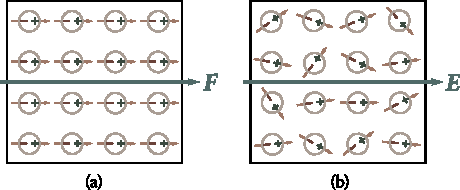
\includegraphics[scale=1]{figures/ch_02/fig_2_1.pdf}
			\caption[]{}
			\label{fig:2_1}
		\end{center}
	\end{minipage}
	\hfill{}%space{-0.05cm}
	\begin{minipage}[t]{0.34\linewidth}
		\begin{center}
			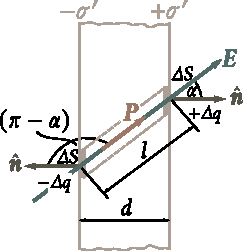
\includegraphics[scale=1]{figures/ch_02/fig_2_2.pdf}
			\caption[]{}
			\label{fig:2_2}
		\end{center}
	\end{minipage}
\vspace{-0.4cm}
\end{figure}

Có một liên hệ đơn giản giữa độ phân cực $\vec{P}$ và mật độ điện tích liên kết mặt $\sigma'$. Để tìm nó, ta  xét một bản mặt song song vô hạn của điện môi đồng chất đặt trong một điện trường đồng nhất (\fig{2_2}). Ta hãy tách ra một thể tích nguyên tố trong bản ở dạng một hình trụ rất mỏng có đường sinh song song với $\vec{E}$ trong điện môi, và có diện tích đáy $\Delta{S}$ trùng với bề mặt bản. Độ lớn của thể tích này là
\begin{equation*}
    \Delta{V} = l \Delta{S} \cos\alpha
\end{equation*}

\noindent
Với $l$ là khoảng cách giữa các đáy của hình trụ và $\alpha$ là góc giữa vector $\vec{E}$ và một ngoại hướng pháp tuyến với bề mặt tích điện dương của điện môi.

Thể tích $\Delta{V}$ có moment lưỡng cực điện với độ lớn
\begin{equation*}
    P\Delta{V} = Pl\Delta{S}\cos\alpha
\end{equation*}

\noindent
($P$ là độ lớn của độ phân cực).

Theo quan điểm vĩ mô, thể tích có thể được xem như tương đương với một lưỡng cực tạo bởi $+\sigma'\Delta{S}$ và $-\sigma'\Delta{S}$ với khoảng cách $l$. Do đó, moment điện của nó có thể được viết ở dạng $\sigma'\Delta{S}l$. Đồng nhất hai biểu thức cho moment điện, ta có
\begin{equation*}
    Pl\Delta{S}\cos\alpha = \sigma'\Delta{S}l.
\end{equation*}

\noindent
Do đó, ta nhận được mối qua hệ cần thiết giữa $\sigma'$ và $\vec{P}$:
\begin{equation}\label{eq:2_9}
    \sigma' = P \cos\alpha = \ab{P}{n}
\end{equation}

\noindent
với $\ab{P}{n}$ là hình chiếu của độ phân cực lên một ngoại hướng pháp tuyến của bề mặt liên quan. Ở bề mặt bên phải trong \fig{2_2}, ta có $\ab{P}{n}>0$, theo đó, $\sigma'$ cho nó là dương; ở bề mặt bên trái $\ab{P}{n}<0$, theo đó, $\sigma'$ của nó là âm.

Biểu diễn $\vec{P}$ qua $\chi$ và $\vec{E}$ bằng \eqn{2_5}, ta được công thức
\begin{equation}\label{eq:2_10}
    \sigma' = \chi \varepsilon_0 \ab{E}{n}
\end{equation}

\noindent
với $\ab{E}{n}$ là thành phần pháp tuyến của cường độ trường bên trong điện môi. Theo \eqn{2_10}, tại nơi đường sức trường đi ra khỏi điện môi ($\ab{E}{n}>0$), điện tích liên kết dương xuất hiện ở bề mặt, trong khi tại nơi đường sức trường đi vào  điện môi ($\ab{E}{n}<0$), điện tích mặt âm xuất hiện.

Phương trình \eqref{eq:2_9} và \eqref{eq:2_10} vẫn đúng trong trường hợp tổng quát nhất khi một điện môi không đồng chất hình dạng bất kỳ đặt trong một điện trường không đồng nhất. Với $\ab{P}{n}$ và $\ab{E}{n}$ trong trường hợp này, ta phải hiểu thành phần pháp tuyến của vector liên quan được lấy gần trực tiếp với bề mặt nguyên tố mà $\sigma'$ được xác định.

Bây giờ ta hãy tìm mật độ khối của điện tích liên kết bên trong điện môi không đồng chất. Xét một diện tích ảo nhỏ $\Delta{S}$ (\fig{2_3}) trong điện môi đẳng hướng không đồng chất với phân tử không phân cực.
Cho rằng một đơn vị thể tích điện môi có $n$ hạt giống hệt nhau với điện tích $+e$ và $n$ hạt giống hệt nhau với điện tích $-e$. Ở gần diện tích $\Delta{S}$, điện trường và điện môi có thể được xem là đồng nhất.
Do đó, khi trường xuất hiện, mọi điện tích dương gần $\Delta{S}$ sẽ dịch chuyển một khoảng cách bằng nhau $l_1$ theo hướng của $\vec{E}$, và mọi điện tích âm sẽ dịch chuyển theo hướng ngược lại cùng một đoạn $l_2$ (xem \fig{2_3}).
Một số điện tích nhất định cùng dấu (dương nếu $\alpha<\pi/2$ và âm nếu $\alpha>\pi/2$) sẽ đi qua diện tích $\Delta{S}$ theo hướng của một pháp tuyến với nó, và một số điện tích nhất định trái dấu (âm nếu $\alpha<\pi/2$ và dương nếu $\alpha<\pi/2$) theo hướng ngược với $\hatvec{n}$.
Diện tích $\Delta{S}$ sẽ bị cắt bởi tất cả tất cả điện tích $+e$ nằm cách nó một khoảng không quá $l_1\cos\alpha$ trước khi trường được bật, tức là, bởi tất cả $+e$ trong hình trụ xiên có thể tích $l_1\Delta{S}\cos\alpha$. Lượng điện tích này là $nl_1\Delta{S}\cos\alpha$, trong khi điện tích chúng mang theo hướng của pháp tuyến tới diện tích là $enl_1\Delta{S}\cos\alpha$ (khi $\alpha>\pi/2$, điện tích được mang theo hướng của pháp tuyến do sự dịch chuyển của điện tích $+e$ là âm).
Tương tự, diện tích $\Delta{S}$ sẽ bị cắt bởi tất cả điện tích $-e$ trong thể tích $l_2\Delta{S}\cos\alpha$. Những điện tích này sẽ mang điện tích $enl_2\Delta{S}\cos\alpha$ theo hướng pháp tuyến của diện tích (từ \fig{2_3} chỉ ra rằng khi $\alpha<\pi/2$, điện tích $-e$ sẽ mang lượng điện tích $-enl_2\Delta{S}\cos\alpha$ qua $\Delta{S}$ theo hướng ngược với $\hatvec{n}$, tương đương với việc mang điện tích $enl_2\Delta{S}\cos\alpha$ theo hướng của $\hatvec{n}$).

\begin{figure}[!htb]
	\begin{center}
		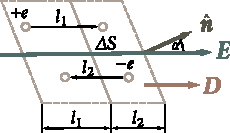
\includegraphics[scale=1.1]{figures/ch_02/fig_2_3.pdf}
		\caption[]{}
		\label{fig:2_3}
	\end{center}
	\vspace{-0.8cm}
\end{figure}

Do đó, khi trường được bật, điện tích
\begin{equation*}
    \Delta{q}' = enl_1\Delta{S}\cos\alpha + enl_2\Delta{S}\cos\alpha = en (l_1+l_2) \Delta{S} \cos\alpha
\end{equation*}

\noindent
được mang qua diện tích $\Delta{S}$ theo hướng pháp tuyến của nó. Tổng $l_1+l_2$ là khoảng cách $l$ mà điện tích liên kết dịch chuyển về phía nhau trong điện môi.Như là kết quả của của sự dịch chuyển này, mỗi cặp điện tích nhận được moment lưỡng cực $p=el=e(l_1+l_2)$. Số cặp trong trong một đơn vị thể tích là $n$. Kết quả là, tích $e(l_1+l_2)n=eln=p$ cho ta độ lớn của độ phân cực $P$. Từ đó, điện tích đi qua diện tích $\Delta{S}$ theo hướng pháp tuyến khi trường được bật là [xem \eqn{2_9}]
\begin{equation*}
    \Delta{q}' = P \Delta{S} \cos\alpha.
\end{equation*}

Vì điện môi đẳng hướng, hướng của vector $\vec{E}$ và $\vec{P}$ trùng nhau (xem \fig{2_3}). Kết quả là, $\alpha$ là góc giữa vector $\vec{P}$ và $\hatvec{n}$, và trong liên hệ này ta có thể viết
\begin{equation*}
    \Delta{q}' = (\vec{P} \ccdot \hatvec{n})\, \Delta{S}.
\end{equation*}

\noindent
Chuyển từ $\Delta$ sang vi phân, ta có
\begin{equation*}
    \deriv{q} = (\vec{P} \ccdot \hatvec{n})\, \deriv{S} = \vec{P} \ccdot \deriv{\vec{S}}.
\end{equation*}

Ta đã tìm được điện tích liên kết $\deriv{q'}$ mà đi qua diện tích nguyên tố $\deriv{S}$ theo hướng pháp tuyển khi trường được bật; $\vec{P}$ là độ phân cực thiết lập dưới tác dụng của điện trường tại vị trí diện tích $\deriv{S}$.

Tưởng tượng một mặt đóng $S$ bên trong điện môi. Khi trường được bật, một điện tích liên kết $q'$ sẽ cắt bề mặt này và đi ra từ nó. Điện tích này là
\begin{equation*}
    \ab{q'}{em} = \oint_S \deriv{q'} = \oint_S \vec{P} \ccdot \deriv{\vec{S}}
\end{equation*}

\noindent
(ta đã đồng ý lấy ngoại hướng pháp tuyến cho diện tích $\deriv{S}$ của mặt kín). Kết quả là, một điện tích liên kết dư sẽ xuất hiện trong thể tích giới hạn bởi bề mặt $S$. Giá trị của nó là
\begin{equation}\label{eq:2_11}
    \ab{q'}{sur} = - \ab{q'}{em} = - \oint_S \vec{P} \ccdot \deriv{\vec{S}} = - \ab{\Phi}{P}
\end{equation}

\noindent
($\ab{\Phi}{P}$ là thông lượng của vector $\vec{P}$ qua mặt $S$).

Đưa vào mật độ điện tích liên kết khối $\rho'$, ta có thể viết
\begin{equation*}
    \ab{q'}{sur} = \int_V \rho'\, \deriv{V}
\end{equation*}

\noindent
(tích phân được lấy trên toàn bộ thể tích giới hạn bởi bề mặt $S$). Chúng ta do đó có được công thức
\begin{equation*}
    \int_V \rho'\, \deriv{V} = - \oint_S \vec{P} \ccdot \deriv{\vec{S}}.
\end{equation*}

\noindent
Biến đổi tích phân mặt theo định lý Ostrogradsky-Gauss [xem \eqn{1_108}). Kết quả là
\begin{equation*}
    \int_V \rho'\, \deriv{V} = - \int_V \divop{\vec{P}}\, \deriv{V}.
\end{equation*}

\noindent
Phương trình này phải được tuân thủ cho bất kì thể tích được chọn tùy ý $V$. Điều này chỉ có thể xảy ra nếu phương trình sau được tuân thủ tại mọi điểm của điện môi:
\begin{equation}\label{eq:2_12}
    \rho' = - \divop{\vec{P}}.
\end{equation}

\noindent
Kết quả là, mật độ điện tích liên kết bằng với divergence của độ phân cực $\vec{P}$ lấy trái dấu.

Ta nhận được \eqn{2_12} khi xét điện môi với phân tử không phân cực. Phương trình này vẫn đúng cho điện môi với phân tử phân cực.

\begin{figure}[!htb]
	\begin{center}
		
\includegraphics[scale=1]{figures/ch_02/fig_2_4.pdf}
		\caption[]{}
		\label{fig:2_4}
	\end{center}
	\vspace{-0.8cm}
\end{figure}

Phương trình \eqref{eq:2_12} có thể giải thích bằng sơ đồ. Các điểm với $\divop{\vec{P}}$ dương là nguồn của trường vector $\vec{P}$, và các đường sức từ $\vec{P}$ phân kì từ chúng (\fig{2_4}). Các điểm với $\divop{\vec{P}}$ âm là phần chìm của trường vector $\vec{P}$, và các đường sức của $\vec{P}$ hội tụ tại chúng.
Trong sự phân cực điện môi, các điện tích liên kết dương dịch chuyển theo hướng của vector $\vec{P}$, tức là, theo hướng của các đường $\vec{P}$; Các điện tích liên kết âm dịch chuyển theo hướng ngược lại (trong hình các điện tích liên kết thuộc về các phân tử riêng biệt được bao quanh bởi hình bầu dục). Kết quả là, sự dư thừa các điện tích liên kết âm được tạo thành tại những điểm có $\divop{\vec{P}}$ dương, và sự dư thừa các điện tích liên kết dương tại nơi có $\divop{\vec{P}}$ âm.
 Điện tích liên kết chỉ khác điện tích ngoài ở chỗ chúng không thể rời khỏi giới hạn phân tử của chúng. Nếu không thì, chúng có cùng đặc tính với toàn bộ điện tích khác. Đặc biệt, chúng là nguồn của một điện trường. Do đó, khi mật độ điện tích liên kết $\rho'$ khác không, \eqn{1_117} phải được viết ở dạng
\begin{equation}\label{eq:2_13}
    \divop{\vec{E}} = \frac{1}{\varepsilon_0} \parenthesis{\rho + \rho'}.
\end{equation}

\noindent
Ở đây $\rho$ là mật độ điện tích ngoài.

Đưa \eqn{2_5} for $\vec{P}$ vào \eqn{2_12} và sử dụng \eqn{1_103}. Kết quả là
\begin{equation*}
    \rho' = - \divop{(\chi\varepsilon_0\vec{E})} = - \varepsilon_0 \divop{(\chi\vec{E})} = - \varepsilon_0 [\vec{E}\ccdot\gradop{\chi} + \chi \divop{\vec{E}}].
\end{equation*}

\noindent
Thay thể $\divop{\vec{E}}$ bằng giá trị của nó từ \eqn{2_13}, ta nhận được phương trình
\begin{equation*}
    \rho' = - \varepsilon_0 (\vec{E}\ccdot\gradop{\chi}) - \chi\rho - \chi\rho'.
\end{equation*}

\noindent
Vì thế,
\begin{equation}\label{eq:2_14}
    \rho' = - \parenthesis{\frac{1}{1+\chi}} [\varepsilon_0 (\vec{E}\ccdot\gradop{\chi}) + \chi\rho].
\end{equation}

Ta có thể thấy từ \eqn{2_14} rằng mật độ điện tích liên kết khối có thể khác không trong hai trường hợp: (1) nếu điện môi không đồng nhất ($\gradop{\chi}\neq 0$), và (2) nếu tại một khu vực cho trước trong điện môi. mật độ điện tích ngoài khác không ($\rho\neq 0$).

Khi không có điện tích ngoài trong điện môi, mật độ điện tích liên kết khối là
\begin{equation}\label{eq:2_15}
    \rho' = - \parenthesis{\frac{\varepsilon_0}{1+\chi}} (\vec{E}\ccdot\gradop{\chi}).
\end{equation}

\section{Vector điện dịch}\label{sec:2_5}

Ta chú ý ở phần trước rằng không chỉ có điện tích ngoài, mà điện tích liên kết cũng là nguồn của trường. Theo,
\begin{equation}\label{eq:2_16}
    \divop{\vec{E}} = \frac{1}{\varepsilon_0} \parenthesis{\rho + \rho'}
\end{equation}

\noindent
[xem \eqn{2_13}].

Phương trình \eqref{eq:2_16} hầu như không dùng để tìm vector $\vec{E}$ bởi vì nó thể hiện đặc tính của đại lượng chưa biết $\vec{E}$ thông qua điện tích liên kết, cái mà được xác định bởi đại lượng $\vec{E}$ chưa biết [xem phương trình \eqref{eq:2_10} và \eqref{eq:2_14}].

Tính toán trường thường được đơn giản hóa khi ta đưa vào một đại lượng phụ mà nguồn của nó chỉ là các điện tích ngoài $\rho$. Để thiết lập đại lượng này trông như thế nào, ta đưa vào \eqn{2_12} của $\rho'$ vào \eqn{2_16}:
\begin{equation*}
    \divop{\vec{E}} = \frac{1}{\varepsilon_0} (\rho - \divop{\vec{P}})
\end{equation*}

\noindent
Theo đó
\begin{equation}\label{eq:2_17}
    \divop{(\varepsilon_0\vec{E} + \vec{P})} = \rho
\end{equation}

\noindent
(Ta đặt $\varepsilon_0$ trong ký hiệu del). Biểu thức trong dấu ngoặc đơn trong \eqn{2_17} là đại lượng cần tìm. Nó được ký hiệu bởi $\vec{D}$ và được gọi là vector điện dịch (hoặc cảm ứng điện).

Do đó, vector \textbf{điện dịch} là một đại lượng xác định bởi liên hệ
\begin{equation}\label{eq:2_18}
    \vec{D} = \varepsilon_0\vec{E} + \vec{P}.
\end{equation}

\noindent
Thay \eqn{2_5} cho $\vec{P}$, ta có
\begin{equation}\label{eq:2_19}
    \vec{D} = \varepsilon_0\vec{E} + \chi\varepsilon_0\vec{E} = \varepsilon_0 (1+\chi) \vec{E}.
\end{equation}

Đại lượng vô hướng
\begin{equation}\label{eq:2_20}
    \varepsilon = 1 + \chi
\end{equation}

\noindent
được gọi là \textbf{hằng số điện môi tương đối} hoặc đơn giản là \textbf{hằng số điện môi} của môi trường\footnote{Cái gọi là hằng số điện môi tuyệt đối của môi trường $\ab{\varepsilon}{a}=\varepsilon_0\varepsilon$ được giới thiệu trong kỹ thuật điện. Đại lượng này bị thiếu đi ý nghĩa vật lý, tuy nhiên, ta sẽ không dùng nó.}. Do đó, \eqn{2_19} có thể được viết ở dạng
\begin{equation}\label{eq:2_21}
    \vec{D} = \varepsilon_0 \varepsilon \vec{E}.
\end{equation}

\noindent
Theo \eqn{2_21}, vector $\vec{D}$ tỷ lệ với vector $\vec{E}$. Nhắc lại cho người đọc rằng chúng ta đang giải quyết với điện môi đẳng hướng. Trong điện môi không đẳng hướng, vector $\vec{E}$ và $\vec{D}$, nói chung, là không thẳng hàng.

Phù hợp với \eqn{1_15} và \eqn{2_21}, vector điện dịch của trường của một điện tích điểm trong chân không là
\begin{equation}\label{eq:2_22}
    \vec{D} = \frac{1}{4\pi} \frac{q}{r^2} \vecuni{r}.
\end{equation}

Đơn vị của độ điện dịch là coulomb trên mét bình phương (\si{\coulomb\per\metre\squared}).

Phương trình \eqref{eq:2_17} có thể được viết như
\begin{equation}\label{eq:2_23}
    \divop{\vec{D}} = \rho.
\end{equation}

\noindent
Tích phân phương trình này trên một thể tích bất kỳ $V$ dẫn đến
\begin{equation*}
    \int_V \divop{\vec{D}}\, \deriv{V} = \int_V \rho\, \deriv{V}.
\end{equation*}

\noindent
Ta hãy biến đổi vế trái theo định lý Ostrogradsky-Gauss [xem \eqn{1_108}]:
\begin{equation}\label{eq:2_24}
    \oint_S \vec{D} \ccdot \deriv{\vec{S}} = \int_V \rho\, \deriv{V}.
\end{equation}

\noindent
Đại lượng bên vế trái là $\Phi_D$---thông lượng của vector $\vec{D}$ qua mặt kín $S$, trong khi đó ở vế phải là tổng điện tích ngoài $\sum_iq_i$ giới hạn bởi bề mặt này. Do đó, \eqn{2_24} có thể được viết ở dạng
\begin{equation}\label{eq:2_25}
    \Phi_D = \sum_i q_i.
\end{equation}

\noindent
Phương trình \eqref{eq:2_24} và \eqref{eq:2_25} thể hiện định luật Gauss cho vector $\vec{D}$: \textit{thông lượng điện dịch qua một mặt kín bằng tổng đại số của điện tích ngoài giới hạn trong mặt này}.

Trong chân không, $\vec{P}=0$, vì vậy đại lượng $\vec{D}$ xác định bởi \eqn{2_18} chuyển thành $\varepsilon_0\vec{E}$, phương trình \eqref{eq:2_24} và \eqref{eq:2_25} chuyển thành phương trình \eqref{eq:1_114} và \eqref{eq:1_116}.

Đơn vị của thông lượng vector điện dịch là coulomb. Xem \eqn{2_25}, một điện tích \SI{1}{\coulomb} tạo ra thông lượng điện dịch \SI{1}{\coulomb} qua bề mặt bao quanh nó.

Trường của vector $\vec{D}$ có thể minh họa bằng các đường điện dịch (ta sẽ gọi chúng là các đường dịch cho ngắn gọn). Hướng và mật độ của chúng được xác định theo cách giống hệt như các đường của vector $\vec{E}$ (xem \sect{1_5}). Các đường của vector $\vec{E}$ có thể bắt đầu và kết thúc tại cả điện tích ngoài và liên kết. Nguồn của trường vector $\vec{D}$ chỉ là điện tích ngoài. Do đó, các đường dịch chỉ có thể bắt đầu và kết thúc tại điện tích ngoài. Những đường này đi qua mà không bị ngắt quãng tại các điểm có điện tích liên kết.

Cảm ứng điện\footnote{Thuật ngữ ``điện dịch'' không áp dụng cho đại lượng \eqref{eq:2_27}.} trong hệ Gauss được xác định bởi biểu thức
\begin{equation}\label{eq:2_26}
    \vec{D} = \vec{E} + 4\pi\vec{P}.
\end{equation}

\noindent
Thay $\vec{P}$ trong phương trình này bằng giá trị của nó trong \eqn{2_6}, ta có
\begin{equation}\label{eq:2_27}
    \vec{D} = (1 + 4\pi\chi) \vec{E}.
\end{equation}

Đại lượng
\begin{equation}\label{eq:2_28}
    \varepsilon = 1 + 4\pi\chi.
\end{equation}

\noindent
được gọi là \textbf{hằng số điện môi}. Đưa đại lượng này vào \eqn{2_27} ta có
\begin{equation}\label{eq:2_29}
    \vec{D} = \varepsilon \vec{E}.
\end{equation}

Trong hệ Gauss, cảm ứng điện trong chân không trùng với điện trường $\vec{E}$. Kết quả là, cảm ứng điện của trường một điện tích điểm trong chân không được xác định bởi \eqn{1_16}.

Theo \eqn{2_22} độ điện dịch tạo bởi điện tích \SI{1}{\coulomb} tại khoảng cách \SI{1}{\metre} là
\begin{equation*}
    D = \frac{1}{4\pi}\frac{q}{r^2} = \frac{1}{4\pi\times 1^2} = \frac{1}{4\pi} \si{\coulomb\per\metre\squared}.
\end{equation*}

\noindent
Trong hệ Gauss, cảm ứng điện trong trường hợp này là
\begin{equation*}
    D = \frac{q}{r^2} = \frac{\num{3e9}}{\num{e4}} = \SI{3e5}{\cgse{D}}.
\end{equation*}

\noindent
Do đó,
\begin{equation*}
    \SI{1}{\coulomb\per\metre\squared} = 4\pi \times  \SI{3e5}{\cgse{D}}.
\end{equation*}

Trong hệ Gauss, biểu thức của định luật Gauss có dạng
\begin{align}
    \oint_S \vec{D} \ccdot \deriv{\vec{S}} &= 4\pi \int_V \rho\, \deriv{V}\label{eq:2_30}\\
    \Phi_D &= 4\pi \sum_i q_i.\label{eq:2_31}
\end{align}

\noindent
Theo \eqn{2_31}, một điện tích \SI{1}{\coulomb} tạo ra một thông lượng của vector cảm ứng điện bằng $4\pi q=4\pi\times\SI{3e9}{\cgse{\Phi_D}}$. Do đó tồn tại mối liên hệ sau giữa các đơn vị của thông lượng của vector $\vec{D}$:
\begin{equation*}
    \SI{1}{\coulomb} = 4\pi \times \SI{3e9}{\cgse{\Phi_D}}.
\end{equation*}

\section{Các ví dụ tính toán điện trường trong điện môi}\label{sec:2_6}

Ta sẽ xem xét một vài ví dụ của điện trường trong điện môi để khám phá ý nghĩa của đại lượng $\vec{D}$ và $\varepsilon$.

\textbf{Trường trong một bản phẳng.} Xét hai mặt phẳng song song vô hạn tích điện trái dấu. Trường chúng tạo ra trong chân không được đặc trưng bởi điện trường $\vec{E}_0$ và điện dịch $\vec{D}_0=\varepsilon_0\vec{E}_0$. Đưa vào trường này một bản điện môi đồng chất đẳng hướng và xếp nó như trong \fig{2_5}. Điện môi phân cực dưới tác dụng của trường, và điện tích liên kết có mật độ mặt $\sigma'$ sẽ xuất hiện trên bề mặt. Những điện tích này sẽ thiết lập một trường đồng nhất bên trong bản mà cường độ của nó theo \eqn{1_121} là $E'=\sigma'/\varepsilon_0$. Trong trường hợp đã cho, $E'=0$ bên ngoài điện môi.

\begin{figure}[!htb]
	\begin{center}
		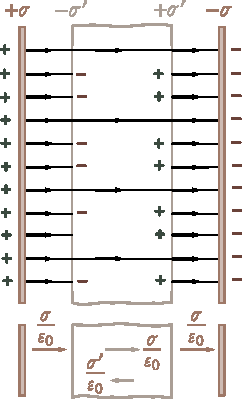
\includegraphics[scale=1]{figures/ch_02/fig_2_5.pdf}
		\caption[]{}
		\label{fig:2_5}
	\end{center}
	\vspace{-0.8cm}
\end{figure}

Cường độ trường $E_0$ bằng $\sigma/\varepsilon_0$. Cả hai trường hướng vào nhau, do đó, bên trong điện môi ta có
\begin{equation}\label{eq:2_32}
    E = E_0 - E' = E_0 - \frac{\sigma'}{\varepsilon_0} = \frac{1}{\varepsilon_0}(\sigma - \sigma').
\end{equation}

\noindent
Bên ngoài điện môi, $E=E_0$.

Độ phân cực của điện môi là do trường \eqref{eq:2_32}. Cái sau vuông góc với mặt bản. Do đó, $\ab{E}{n}=E$, và phù hợp với \eqn{2_10}, $\sigma'=\chi\varepsilon_0E$. Sử dụng giá trị này trong \eqn{2_32}, ta có
\begin{equation*}
    E = E_0 - \chi E
\end{equation*}

\noindent
từ đó
\begin{equation}\label{eq:2_33}
    E = \frac{E_0}{1 + \chi} = \frac{E_0}{\varepsilon}.
\end{equation}

\noindent
Vì vậy, trong trường hợp này, hằng số điện môi $\varepsilon$
chỉ ra điện trường bị yếu đi bao nhiêu lần trong điện môi.

Nhân \eqn{2_33} với $\varepsilon_0\varepsilon$, ta có độ điện dịch trong bản:
\begin{equation}\label{eq:2_34}
    D = \varepsilon_0 \varepsilon E = \varepsilon_0 E_0 D_0.
\end{equation}

\noindent
Do đó, độ điện dịch bên trong bản trùng với độ điện dịch của trường ngoài $D_0$. Thay $\sigma/\varepsilon_0$ cho $E_0$ trong \eqn{2_34}, ta được
\begin{equation}\label{eq:2_35}
    D = \sigma.
\end{equation}

Để tìm $\sigma'$, biểu diễn $E$ và $E_0$ trong \eqn{2_33} qua mật độ điện tích:
\begin{equation*}
    \frac{1}{\varepsilon_0} (\sigma - \sigma') = \frac{\sigma}{\varepsilon_0\varepsilon}
\end{equation*}

\noindent
từ đó
\begin{equation}\label{eq:2_36}
    \sigma' = \frac{\varepsilon - 1}{\varepsilon} \sigma.
\end{equation}

Hình \ref{fig:2_5} được vẽ với giả sử $\varepsilon=3$. Do đó, mật độ của đường sức trong điện môi bằng một phần ba bên ngoài bản. Các đường sức cách đều nhau vì trường là đồng nhất. Trong trường hợp này, $\sigma'$ có thể tìm được mà không cần dùng đến \eqn{2_36}. Đúng vậy, vì cường độ điện trường bên trong bản bằng một phần ba cường độ bên ngoài nó, nên ba đường sức bắt đầu (hoặc kết thúc) trên
điện tích ngoài, hai đường phải kết thúc (hoặc bắt đầu tương ứng) trên điện tích liên kết. Do đó mật độ điện tích liên kết phải bằng hai phần ba mật độ điện tích ngoài.

Trong hệ Gauss, cường độ điện trường $E'$ tạo ra bởi điện tích liên kết $\sigma'$ là $4\pi\sigma'$. Do đó, \eqn{2_32} trở thành
\begin{equation}\label{eq:2_37}
    E = E_0 - E' = E_0 - 4\pi\sigma'.
\end{equation}

\noindent
Mật độ điện mựt $\sigma'$ liên hệ với cường độ điện trường $E$ theo phương trình $\sigma'=\chi \ab{E}{n}$. Do đó ta có thể viết
\begin{equation*}
    E = E_0 - 4\pi\chi E
\end{equation*}

\noindent
từ đó
\begin{equation*}
    E = \frac{E_0}{1 + 4\pi\chi} = \frac{E_0}{\varepsilon}.
\end{equation*}

\noindent
Do đó, hằng số điện môi $\varepsilon$, như đối tác của nó $\varepsilon$ trong hệ SI, cho biết trường bên trong điện môi bị yếu đi bao nhiêu lần. Do đó, giá trị của $\varepsilon$ trong hệ SI và hệ Gauss là như nhau. Từ đây, tính đến Eqs. \eqref{eq:2_20} và \eqref{eq:2_28}, ta kết luận rằng độ cảm điện trong hệ Gauss ($\ab{\chi}{Gs}$) và trong hệ SI ($\ab{\chi}{SI}$) khác nhau bởi hệ số $4\pi$:
\begin{equation}\label{eq:2_38}
    \ab{\chi}{SI} = 4\pi\ab{\chi}{Gs}.
\end{equation}

\textbf{Trường bên trong một lớp cầu.} Bao bọc một quả cầu tích điện bán kính $R$ bằng một lớp cầu đồng tâm của điện môi đồng chất đẳng hướng (\fig{2_6}). Điện tích liên kết $q_1'$ phân bố với mật độ $\sigma_1'$ sẽ xuất hiện trên mặt trong của lớp ($q_1'=4\pi R_1^2\sigma_1'$), và điện tích $q_2'$ phân bố với mật độ $\sigma_2'$ sẽ xuất hiện trên mặt ngoài của nó ($q_2'=4\pi R_2^2\sigma_2'$). Dấu của điện tích $q_2'$ trùng với dấu của điện tích $q$ của quả cầu, trong khi đó $q_1'$ trái dấu.
Các điện tích $q_1'$ và $q_2'$ tạo ra một trường tại khoảng cách $r$ bên ngoài $R_1$ và $R_2$, tương ứng, nó trùng với trường của một điện tích điểm cùng độ lớn [xem \eqn{1_124}]. Điện tích $q_1'$ và $q_2'$ không tạo ra trường bên trong bề mặt mà nó được phân bố. Do đó, cường độ trường $E'$ trong điện môi là
\begin{equation*}
    E' = \frac{1}{4\pi\varepsilon_0}\frac{q_1'}{r^2} = \frac{1}{4\pi\varepsilon_0} \frac{4\pi R_1^2\sigma_1'}{r^2} = \frac{1}{\varepsilon_0} \frac{R_1^2 \sigma_1'}{r^2}
\end{equation*}

\noindent
và ngược hướng với cường độ trường $E_0$. Trường tổng hợp trong điện môi là
\begin{equation}\label{eq:2_39}
    E(r) = E_0 - E' = \frac{1}{4\pi\varepsilon_0} \frac{q}{r^2} - \frac{1}{\varepsilon_0} \frac{R_1^2 \sigma_1'}{r^2}.
\end{equation}

\begin{figure}[!htb]
	\begin{center}
		\includegraphics[scale=1.0]{figures/ch_02/fig_2_6.pdf}
		\caption[]{}
		\label{fig:2_6}
	\end{center}
	\vspace{-0.8cm}
\end{figure}

\noindent
Nó giảm tỷ lệ với $1/r^2$. Chúng ta có thể, do đó, viết
\begin{equation*}
    \frac{E(R_1)}{E(r)} = \frac{r^2}{R_1^2}\quad \Rightarrow\quad E(R_1) = E(r) \frac{r^2}{R_1^2},
\end{equation*}

\noindent
với $E(R_1)$ là cường độ điện trường trong điện môi gần với mặt trong của lớp. Chính xác là cường độ này xác định đại lượng $\sigma_1'$:
\begin{equation}\label{eq:2_40}
    \sigma_1' = \chi\varepsilon_0 E(R_1) = \chi\varepsilon_0 E(r) \frac{r^2}{R_1^2}
\end{equation}

\noindent
(tại môi điểm của bề mặt $|\ab{E}{n}|=E$).

Đưa \eqn{2_40} vào \eqn{2_39}, ta có
\begin{equation*}
    E(r) = \frac{1}{4\pi\varepsilon_0} \frac{q}{r^2} - \frac{1}{\varepsilon_0} \frac{R_1^2 \chi \varepsilon_0 E(r) r^2}{r^2 R_1^2} = E_0(r) - \chi E(r).
\end{equation*}

\noindent
Từ phương trình này, ta thấy rằng bên trong điện môi $E=E_0/\varepsilon$, và, do đó, $D=\varepsilon_0E_0$ [so sánh với phương \eqref{eq:2_33} và \eqref{eq:2_34}].

Trường bên trong điện môi thay đổi tỷ lệ với $1/r^2$. Do đó, có liên hệ $\sigma_1' :\sigma_2' = R_1 : R_2$. Từ đó,  $q_1'=q_2'$. Kết quả là, trường tạo bởi những điện tích này tại khoảng cách quá $R_2$ triệt tiêu lẫn nhau vì thế bên ngoài lớp cầu $E'=0$ và $E=E_0$.

Giả sử rằng $R_1=R$ và $R_2=\infty$, ta được trường hợp của một quả cầu tích điện chìm trong điện môi đồng nhất vô hạn và đẳng hướng. Cường độ trường bên ngoài quả cầu là
\begin{equation}\label{eq:2_41}
    E = \frac{1}{4\pi\varepsilon_0} \frac{q}{\varepsilon r^2}.
\end{equation}

\noindent
Cường độ điện trường tạo ra trong điện môi vô hạn bởi một điện tích điểm cũng tương tự.

Cả hai ví dụ xem xét trên được đặc trưng với thực tế rằng điện môi là đồng nhất và đẳng hướng, và bề mặt giới hạn nó trùng với mặt đẳng thế của điện trường của điện tích ngoài. Kết quả ta nhận được trong trường hợp này là trường hợp tổng quát. \textit{Nếu điện môi đồng nhất và đẳng hướng hoàn toàn lấp đầy thể tích giới hạn bởi bề mặt đẳng tích của trường của điện tích ngoài, thì vector điện dịch trùng với vector của cường độ điện trường của điện tích ngoài nhân với $\varepsilon_0$, và, do đó, cường độ trường bên trong điện môi là $1/\varepsilon$ của cường độ trường của điện tích ngoài}.

Nếu các điều kiện trên không được tuân thủ, vector $\vec{D}$ và $\varepsilon_0\vec{E}$ không trùng nhau. Hình \ref{fig:2_7} biểu diễn trường trong bản điện môi. Bản lệch so với mặt phẳng mang điện tích ngoài. Vector $\vec{E}'$ vuông góc với mặt bản, do đó, $\vec{E}$ và $\vec{E}_0$ là không thẳng hàng. Vector $\vec{D}$ có hướng giống $\vec{E}$, do đó, $\vec{D}$ và $\varepsilon_0\vec{E}_0$ không cùng hướng. Ta cũng có thể chỉ ra rằng chúng không cùng độ lớn.
Ở ví dụ được xem xét ở trên nhờ hình dạng được chọn đặc biệt của điện môi, trường $\vec{E}'$ chỉ khác không ở trong điện môi. Trong trường hợp tổng quát, $\vec{E}'$ có thể khác không cả ở bên ngoài điện môi. Ta đặt một thanh làm bằng điện môi vào một trường đồng chất ban đầu (\fig{2_8}). Do sự phân cực, điện tích liên kết trái dấu tạo thành ở hai đầu thanh. Trường của chúng bên ngoài thanh tương đương với trường của một lưỡng cực (các đường sức của $\vec{E}'$ là các đường nét đứt trong hình). Dễ thấy rằng trường tổng cộng $\vec{E}$ gần các đầu thanh lớn hơn trường $\vec{E}_0$.

\begin{figure}[!htb]
	\begin{minipage}[t]{0.46\linewidth}
		\begin{center}
			\includegraphics[scale=1.2]{figures/ch_02/fig_2_7.pdf}
			\caption[]{}
			\label{fig:2_7}
		\end{center}
	\end{minipage}
	\hfill{}%space{-0.05cm}
	\begin{minipage}[t]{0.5\linewidth}
		\begin{center}
			\includegraphics[scale=1.2]{figures/ch_02/fig_2_8.pdf}
			\caption[]{}
			\label{fig:2_8}
		\end{center}
	\end{minipage}
\vspace{-0.4cm}
\end{figure}

\section{Các điều kiện trên mặt phân cách hai điện môi}\label{sec:2_7}

Gần mặt phân cách giữa hai điện môi, vector $\vec{E}$ và $\vec{D}$ phải tuân theo điều kiện biên xác định từ quan hệ \eqref{eq:1_112} và \eqref{eq:2_23}:
\begin{equation*}
    \curlop{\vec{E}} = 0,\quad \divop{\vec{D}} = \rho.
\end{equation*}

Xét bề mặt phân cách giữa hai điện môi với hằng số điện môi $\varepsilon_1$ và $\varepsilon_2$ (\fig{2_9}). Chọn trục $x$ hướng bất kì trên bề mặt. Ta lấy một chu tuyến hình chữ nhật nhỏ dài $a$ và rộng $b$ mà một phần trong điện môi thứ nhất và một phần trong điện môi thứ hai. Trục $x$ đi qua trung điểm của cạnh $b$.

Giả sử rằng một trường đã được thiết lập trong điện môi thứ nhất có cường độ $\vec{E}_1$, và trong điện môi thứ hai có cường độ $\vec{E}_2$. Vì $\curlop{\vec{E}}=0$, lưu số của vector $\vec{E}$ trên chu tuyến ta đã chọn phải bằng không [xem \eqn{1_110}]. Với kích thước nhỏ của chu tuyến và hướng của chu tuyến trong \fig{2_9}, lưu số của vector $\vec{E}$ có thể được viết ở dạng
\begin{equation}\label{eq:2_42}
    \oint E_l\,\deriv{l} = E_{1,x} a - E_{2,x} a + \average{E_b} 2b
\end{equation}

\noindent
với $\average{E_b}$ là giá trị trung bình của $E_l$ trên phần vuông góc mặt phân cách của chu tuyến. Biểu thức này bằng không, ta được phương trình
\begin{equation*}
    \parenthesis{E_{1,x} - E_{2,x}} a = \average{E_b} 2b.
\end{equation*}

\noindent
Trong giới hạn, khi độ rộng $b$ của chu tuyến tiến tới không, ta có
\begin{equation}\label{eq:2_43}
    E_{1,x} = E_{2,x}.
\end{equation}

\noindent
Giá trị của hình chiếu vector $\vec{E}_1$ và $\vec{E}_2$ lên trục $x$ được lấy ở lân cận mặt phân cách giữa ranh giới của các điện môi.

Phương trình \eqref{eq:2_43} được tuân thủ khi trục $x$ được chọn tùy ý. Chỉ có một điều quan trọng là trục này ở trong mặt phẳng phân cách giữa các điện môi. Nghiên cứu \eqn{2_43} chỉ ra rằng với trục $x$ được chọn như thế thì $E_{1,x}=0$, hình chiếu của $E_{2,x}=0$ cũng sẽ bằng không. Điều này có nghĩa là vector $\vec{E}_1$ và $\vec{E}_2$ tại hai điểm gần nhau được lấy ở hai phía đối diện của mặt phân cách là nằm trong cùng mặt phẳng với pháp tuyến của mặt phân cách. Biểu diễn mỗi vector $\vec{E}_1$ và $\vec{E}_2$ ở dạng tổng các thành phần pháp tuyến và tiếp tuyến:
\begin{equation*}
    \vec{E}_1 = \vec{E}_{1,n} + \vec{E}_{1,\tau},\quad \vec{E}_2 = \vec{E}_{2,n} + \vec{E}_{2,\tau}.
\end{equation*}

\noindent
Phù hợp với \eqn{2_43}
\begin{equation}\label{eq:2_44}
    E_{1,\tau} = E_{2,\tau}.
\end{equation}

\noindent
Ở đây $\vec{E}_{i,\tau}$ là hình chiếu của vector $\vec{E}_i$ lên vector đơn vị $\hatvec{\tau}$ hướng dọc theo giao tuyến của mặt phân cách điện môi với mặt phẳng chứa vector $\vec{E}_1$ và $\vec{E}_2$.

\begin{figure}[!htb]
	\begin{minipage}[t]{0.48\linewidth}
		\begin{center}
			\includegraphics[scale=1.0]{figures/ch_02/fig_2_9.pdf}
			\caption[]{}
			\label{fig:2_9}
		\end{center}
	\end{minipage}
	\hfill{}%space{-0.05cm}
	\begin{minipage}[t]{0.48\linewidth}
		\begin{center}
			\includegraphics[scale=1.0]{figures/ch_02/fig_2_10.pdf}
			\caption[]{}
			\label{fig:2_10}
		\end{center}
	\end{minipage}
\vspace{-0.4cm}
\end{figure}

Thay thế phù hợp với \eqn{2_21} Hình chiếu của vector $\vec{D}$ chia $\varepsilon_0\varepsilon$ cho hình chiếu của vector $\vec{E}$, ta có tỷ lệ
\begin{equation*}
    \frac{D_{1,\tau}}{\varepsilon_0\varepsilon_1} = \frac{D_{2,\tau}}{\varepsilon_0\varepsilon_2}
\end{equation*}

\noindent
do đó
\begin{equation}\label{eq:2_45}
    \frac{D_{1,\tau}}{D_{2,\tau}} = \frac{\varepsilon_1}{\varepsilon_2}.
\end{equation}

Bây giờ ta lấy một mặt trụ ảo chiều cao $h$ trên mặt phân cách giữa giữa các điện môi (\fig{2_10}). Đáy $S_1$ nằm trong điện môi thứ nhất, và đáy $S_2$ trong cái thứ hai. Hai đáy có kích thước giống nhau ($S_1=S_2=S$) và nhỏ tới mức mà trong giới hạn của chúng, trường có thể xem là đồng nhất. Áp dụng định lý Gauss [xem \eqn{2_25}] vào mặt này. Nếu không có điện tích ngoài trên mặt phân cách giữa các điện môi, vế phải trong \eqn{2_25} bằng không. Do đó, $\Phi_D=0$.

Thông lượng qua mặt $S_1$ là $D_{1,n}S$, với $D_{1,n}$ là hình chiếu của vector $\vec{D}$ trong điện môi thứ nhất lên pháp tuyến $\hatvec{n}_1$. Tương tự, thông lượng qua đáy $S_2$ là $D_{2,n}S$, với $D_{2,n}$ là hình chiếu của vector $\vec{D}$ trong điện môi thứ hai lên pháp tuyến $\hatvec{n}_2$. Thông lượng qua
mặt bên có thể được viết ở dạng $\average{D}_n\ab{S}{side}$, với $\average{D}_n$ là giá trị của $D_n$ trung bình trên toàn bộ mặt bên, và $\ab{S}{side}$ là độ lớn của mặt này. Do đó có thể viết
\begin{equation}\label{eq:2_46}
    \Phi_D = D_{1,n} S + D_{2,n} S + \average{D}_n\ab{S}{side} = 0.
\end{equation}

\noindent
Nếu độ cao $h$ của hình trụ tiến tới không, thì $\ab{S}{side}$ cũng tiến tới không. Do đó, trong giới hạn, ta có
\begin{equation*}
    D_{1,n} = - D_{2,n}.
\end{equation*}

\noindent
Ở đây $D_{i,n}$ là hình chiếu lên $\hatvec{n}_i$ của vector $\vec{D}$ trong điện môi thứ $i$ ở rất gần mặt phân cách của nó với điện môi khác. Dấu của hình chiếu khác nhau vì pháp tuyến $\hatvec{n}_1$ và $\hatvec{n}_2$ của đáy hình trụ ngược hướng. Nếu ta chiếu $\vec{D}_1$ và $\vec{D}_2$ lên cùng pháp tuyến, ta có điều kiện
\begin{equation}\label{eq:2_47}
    D_{1,n} = D_{2,n}.
\end{equation}

Sử dụng \eqn{2_21} để thay thế hình chiếu của $\vec{D}$ với hình chiếu tương ứng của vector $\vec{E}$ nhân bởi $\varepsilon_0\varepsilon$, ta có liên hệ
\begin{equation*}
    \varepsilon_0 \varepsilon_1 E_{1,n} = \varepsilon_0 \varepsilon_2 E_{2,n}
\end{equation*}

\noindent
do đó
\begin{equation}\label{eq:2_48}
    \frac{E_{1,n}}{E_{2,n}} = \frac{\varepsilon_2}{\varepsilon_1}.
\end{equation}

Kết quả ta nhận được chỉ ra rằng khi đi qua mặt phân cách giữa hai điện môi, thành phần pháp tuyến của vector $\vec{D}$ và thành phần pháp tuyến của vector $\vec{E}$ thay đổi liên tục. Tuy nhiên, thành phần tiếp tuyến của vector $\vec{D}$ và thành phần
pháp tuyến của vector $\vec{E}$, bị gián đoạn khi đi qua mặt phân cách.

Phương trình \eqref{eq:2_44}, \eqref{eq:2_45}, \eqref{eq:2_47}, và \eqref{eq:2_48} xác định các điều kiện mà vector $\vec{E}$ và $\vec{D}$ phải tuân theo trên mặt phân cách giữa hai điện môi (nếu không có điện tích ngoài trên mặt phân cách này). Ta đã nhận được những phương trình này cho một trường tĩnh điện. Chúng cũng đúng cho trường thay đổi theo thời gian (xem
\sect{16_3}).

Các điều kiện ta đã tìm được vẫn đúng cho mặt phân cách giữa điện môi và chân không. Trong trường hợp này, một trong các hằng số điện môi phải bằng một đơn vị.

Ta phải chú ý rằng điều kiện \eqref{eq:2_47} có thể nhận được trên cơ sở của sự thật rằng các đường điện dịch đi qua mặt phân cách giữa hai điện môi mà không bị gián đoạn (\fig{2_11}). Theo
các nguyên tắc để vẽ những đường này, số đường sức tới diện tích $\Delta{S}$ từ điện môi thứ nhất là $D_1\Delta{S}_1=D_1\Delta{S}\cos\alpha_1$. Tương tự, số đường sức đi ra từ diện tích $\Delta{S}$ vào điện môi thứ hai là $D_2\Delta{S}_2=D_2\Delta{S}\cos\alpha_2$. Nếu các đường sức không bị gián đoạn tại mặt phân cách, cả hai số này phải bằng nhau:
\begin{equation*}
    D_1\Delta{S}\cos\alpha_1 = D_2\Delta{S}\cos\alpha_2.
\end{equation*}

\noindent
Rút gọn $\Delta{S}$ và tính đến tích $D\cos\alpha$ cho giá trị của thành phần pháp tuyến vector $\vec{D}$, ta nhận được điều kiện \eqref{eq:2_47}.

Các đường điện dịch bị cong (khúc xạ) trên mặt phân cách giữa các điện môi, do góc $\alpha$ giữa pháp tuyến với mặt phân cách và đường $\vec{D}$ thay đổi. \fig{2_12} chỉ ra rằng
\begin{equation*}
    \tan\alpha_1 : \tan\alpha_2 = \frac{D_{1,\tau}}{D_{1,n}} : \frac{D_{2,\tau}}{D_{2,n}}
\end{equation*}

\noindent
Từ các phương trình \eqref{eq:2_45} và \eqref{eq:2_47}, ta có định luật của sự khúc xạ điện dịch:
\begin{equation}\label{eq:2_49}
    \frac{\tan\alpha_1}{\tan\alpha_2} = \frac{\varepsilon_1}{\varepsilon_2}.
\end{equation}

\noindent
Khi các đường điện dịch đi vào một điện môi với hằng số điện môi $\varepsilon$ bé hơn, góc tạo bởi chúng với pháp tuyến giảm, do đó, các đường cách xa nhau; trái lại, khi các đường đi vào một điện môi với hằng số điện môi $\varepsilon$ lớn hơn, chúng trở nên gần nhau hơn.

\begin{figure}[!htb]
	\begin{minipage}[t]{0.48\linewidth}
		\begin{center}
			\includegraphics[scale=1.1]{figures/ch_02/fig_2_11.pdf}
			\caption[]{}
			\label{fig:2_11}
		\end{center}
	\end{minipage}
	\hfill{}%space{-0.05cm}
	\begin{minipage}[t]{0.48\linewidth}
		\begin{center}
			\includegraphics[scale=1.1]{figures/ch_02/fig_2_12.pdf}
			\caption[]{}
			\label{fig:2_12}
		\end{center}
	\end{minipage}
\vspace{-0.4cm}
\end{figure}

\section{Lực tác dụng lên một điện tích trong điện môi}\label{sec:2_8}

Nếu ta đưa vào điện trường trong chân không một vật mang điện có kích thước nhỏ tới nỗi mà trường ngoài trong vật thể có thể được coi là đồng nhất, thì vật thể sẽ chịu lực
\begin{equation}\label{eq:2_50}
    \vec{F} = q \vec{E}.
\end{equation}

\noindent
Để đặt một vật mang điện trong trường được tạo ra trong một điện môi, phải có một cái hốc trong điện môi. Trong một điện môi lỏng, vật mang điện tự nó tạo hốc bằng cách dịch chuyển điện môi khỏi thể tích nó chiếm. Trường bên trong hốc $\ab{\vec{E}}{cav}$ sẽ khác với với trường trong một điện môi liên tục. Do đó, ta không thể tính lực tác dụng lên vật mang điện đặt trong hốc như là tích của điện tích $q$ và cường độ trường $\vec{E}$ trong điện môi trước khi vật thể được đưa vào nó.

Khi tính lực tác dụng lên một vật mang điện trong điện môi lỏng, ta phải tính đến các trường hợp khác. Sức căng cơ học được thiết lập trên ranh giới với vật thể trong điện môi. Nó tạo ra một lực cơ học phụ $\ab{\vec{F}}{ten}$ tác dụng lên vật thể.

Do đó, lực tác dụng lên một vật mang điện trong điện môi, nói chung, không thể được xác định bởi \eqn{2_50}, và nó thường rất khó để tính toán. Những tính toán này cho một kết quả rất thú vị đối với một điện môi lỏng. Kết quả của lực điện $q\ab{\vec{E}}{cav}$ và lực cơ học $\ab{\vec{F}}{ten}$ được tìm thấy bằng chính xác với $q\vec{E}$, với $\vec{E}$ là cường độ trường trong điện môi liên tục
\begin{equation}\label{eq:2_51}
    \vec{F} = q\ab{\vec{E}}{cav} + \ab{\vec{F}}{ten} = q\vec{E}.
\end{equation}

Cường độ trường trong điện môi đồng chất vô hạn tạo ra bởi một điện tích được xác định bởi \eqn{2_49}. Do đó, ta có biểu thức sau cho lực tương tác giữa hai điện tích điểm chìm trong điện môi đồng chất vô hạn:
\begin{equation}\label{eq:2_52}
    F = \frac{1}{4\pi\varepsilon_0} \frac{q_1q_2}{\varepsilon r^2}.
\end{equation}

\noindent
Công thức này thể hiện định luật Coulomb cho điện tích trong điện môi. Nó chỉ đúng cho điện môi điện môi lỏng.

Một vài tác giả đặc trưng \eqn{2_52} như ``biểu thức tổng quát nhất của định luật coulomb''. Trong vấn đề này, ta sẽ đề cập đến Richard P. Feynman: ``Nhiều cuốn sách cũ hơn về điện bắt đầu với định luật 'quan trọng' mà lực giữa hai điện tích là\ldots [\eqn{2_52} được cho]\ldots, Một quan điểm mà hoàn toàn không thỏa đáng. Đầu tiên, nó không đúng về mặt tổng quát; nó chỉ đúng cho môi trường lấp đầy bởi chất lỏng. Thứ hai, nó phụ thuộc vào sự thật rằng $\varepsilon$ là một hằng số chỉ xấp xỉ đúng cho hầu hết vật liệu thực tế''\footnote{R. P. Feynman, R. B. Leighton, M. Sands. The Feynman Lectures on Physics. Vol. II. Reading, Mass., Addison-Wesley (1965), p. 10-8.}.

Ta sẽ không trả lời câu hỏi liên quan đến lực tác dụng lên một điện tích nằm trong một cái hốc làm từ điện môi rắn.

\section{Sắt điện}\label{sec:2_9}

Có một nhóm vật liệu có thể có tính chất phân cực tự phát khi không có trường ngoài. Chúng được gọi là \textbf{sắt điện}. Hiện tượng này lần đầu tiên được phát hiện ở muối Rochelle, và nghiên cứu cụ thể đầu tiên về tính chất điện của muối này được thực hiện bởi nhà vật lý người Liên Xô I. Kurchatov và P. Kobeko.

Chất sắt điện khác các điện môi ở một số đặc điểm :

1. Trong khi hằng số điện môi $\varepsilon$ của điện môi bình thường chỉ vài đơn vị, một số ngoại lệ lớn (ví dụ, nước có $\varepsilon=81$), hằng số điện môi của chất sắt điện có thể có bậc cỡ vài nghìn.

2. Sự phụ thuộc của $P$ vào $E$ là không tuyến tính (xem nhánh $1$ của đường cong trong \fig{2_13}). Do đó, hằng số điện môi phụ thuộc vào cường độ trường.

3. Khi trường thay đổi, giá trị của độ phân cực $P$ (và, do đó, của điện dịch $D$) trễ pha so với cường độ trường $E$. Kết quả là, $P$ và $D$ được xác định không chỉ bởi giá trị của $E$ tại thời điểm đó, mà còn vào giá trị trước đó của $E$, tức là, chúng phụ thuộc vào trạng thái trước đó của điện môi. Hiện tượng này gọi là \textbf{điện trễ} (từ tiếng Hy Lạp ``husterein''---nghĩa là tới trễ). Khi trường thay đổi tuần hoàn, sự phụ thuộc của $P$ vào $E$  tuân theo đường cong trong \fig{2_13} và được gọi là  \textbf{lặp điện trễ}.
Khi trường bắt đầu xuất hiện, độ phân cực tăng với $E$ theo nhánh $1$ của đường cong. $P$ giảm dọc theo nhánh $2$. Khi $E$ biến mất, vật liệu giữ lại một giá trị của độ phân cực $\ab{P}{r}$ gọi là \textbf{độ phân cực dư}. Độ phân cực chỉ biến mất dưới tác động của một trường hướng ngược lại $\ab{E}{c}$. Giá trị này của cường độ trường gọi là \textbf{lực cưỡng bức}. Khi $E$ thay đổi hơn nữa, ta nhận được nhánh $3$ của vòng lặp điện trễ, vân vân.

\begin{figure}[!htb]
    \begin{center}
		\includegraphics[scale=1.0]{figures/ch_02/fig_2_13.pdf}
		\caption[]{}
		\label{fig:2_13}
	\end{center}
    \vspace{-0.8cm}
\end{figure}

Hành vi của sự phân cực của chất sắt điện là tương tự với sự từ hóa của chất sắt từ (xem \sect{7_9}), và đó là nguồn gốc cái tên của nó.

Chỉ có chất kết tinh không có tâm đối xứng mới có thể là chất sắt điện. Ví dụ, tinh thể của muối Rochelle thuộc hệ hình thoi (xem Sec. 13.2 of Vol. I). Tương tác của các hạt trong tinh thể sắt điện dẫn đến sự thật rằng moment lưỡng cực của chúng xếp song song tự phát với cái khác. Trong các trường hợp riêng biệt, hướng giống nhau của moment lưỡng cực mở rộng ra toàn bộ tinh thể. Tuy nhiên, thông thường, các vùng xuất hiện trong tinh thể mà trong đó moment lưỡng cực là song song với nhau, nhưng các hướng của sự phân cực trong các vùng khác nhau là khác nhau. Do đó, moment tổng cộng của toàn bộ tinh thể có thể bằng không. Vùng có sự phân cực tự phát còn được gọi là \textbf{miền}. Dưới tác dụng của trường ngoài, moment của vùng xoay như một tổng thể duy nhất, sắp xếp chúng theo hướng của trường.

Mỗi chất sắt điện có một nhiệt độ mà tại đó vật chất mất đặc tính khác biệt của nó và trở thành điện môi bình thường. Nhiệt độ này được gọi là \textbf{điểm Curie }. Muối Rochelle có hai điểm Curie, cụ thể là, \SI{-15}{\degreeCelsius} và \SI{+22}{\degreeCelsius}, và nó chỉ biểu hiện như chất sắt điện giữa hai nhiệt độ này. Đặc tính điện của nó trở nên bình thường tại nhiệt độ dưới \SI{-15}{\degreeCelsius} và trên \SI{+22}{\degreeCelsius}.

\cleardoublepage
%% !TEX root = saveliev_physics_general_course_2.tex
%!TEX TS-program = pdflatex
%!TEX encoding = UTF-8 Unicode


\chapter[CONDUCTORS IN AN ELECTRIC FIELD]{CONDUCTORS IN AN ELECTRIC \\FIELD}\label{chap:3}
\chaptermark{VẬT DẪN TRONG ĐIỆN TRƯỜNG}


\section{Cân bằng điện tích trên vật dẫn}\label{sec:3_1}

Các hạt mang điện trong vật dẫn có thể chuyển động dưới tác dụng của một lực rất nhỏ. Do đó, phải có các điều kiện sau đây để các điện tích trên vật dẫn cân bằng:
\begin{enumerate}[1.]
    \item Cường độ trường tại mọi nơi bên trong vật dẫn phải bằng không:
    \begin{equation}\label{eq:3_1}
        \vec{E} = 0.
    \end{equation}

    \noindent
    Phù hợp với \eqn{1_41}, điều này chỉ ra rằng điện thế bên trong vật dẫn phải là hằng số ($\varphi=\text{constant}$).

    \item Điện trường trên bề mặt vật dẫn phải hướng dọc theo pháp tuyến bề mặt tại mọi điểm:
    \begin{equation}\label{eq:3_2}
        \vec{E} = \vec{E}_n.
    \end{equation}

    \noindent
    Kết quả là, khi các điện tích ở trạng thái cân bằng, bề mặt vật dẫn là một mặt đẳng thế.
\end{enumerate}

Nếu một điện tích $q$ được truyền cho một vật dẫn, điện tích sẽ phân bố sao cho đạt được điều kiện cân bằng. Ta hãy tưởng tượng một bề mặt đóng kín tùy ý bị giới hạn hoàn toàn trong một vật. Khi các điện tích cân bằng, không có điện trường tại mọi điểm trong vật dẫn; do đó, thông lượng của vector điện dịch qua bề mặt biến mất. Theo định lý Gauss, tổng điện tích bên trong bề mặt cũng phải bằng không. Điều này đúng cho bề mặt có kích thước bất kỳ được sắp xếp tùy ý bên trong vật dẫn. Từ đó, khi cân bằng, không thể có điện tích dư nào bên trong vật dẫn---tất cả chúng sẽ được phân bố trên bề mặt vật dẫn với mật độ nhất định $\sigma$.

Vì không có điện tích dư trong vật dẫn ở trạng thái cân bằng, việc loại bỏ vật chất từ một thể tích bên trong vật dẫn sẽ không có ảnh hưởng gì đến phân bố cân bằng của điện tích. Do đó, một điện tích dư sẽ được phân bố trên một vật dẫn rỗng giống như một vật dẫn đặc, tức là, dọc theo mặt ngoài của nó. Không có điện tích dư phân bố trên bề mặt của một cái hốc ở trạng thái cân bằng. Kết luận này tuân theo thức tế rằng các điện tích nguyên tố tạo thành điện tích đã cho $q$ đẩy lẫn nhau và, kết quả là, có xu hướng chiếm các vị trí xa nhau nhất.

Tưởng tượng một mặt trụ nhỏ tạo bởi pháp tuyến của bề mặt một vật dẫn và độ lớn đáy $\deriv{S}$, một đáy bên trong và cái còn lại bên ngoài vật dẫn (\fig{3_1}). Thông lượng của vector điện dịch qua phần trong của bề mặt bằng không vì $\vec{E}$ và, do đó, $\vec{D}$ không có trong vật dẫn. Bên ngoài vật dẫn ở gần nó, cường độ trường $\vec{E}$ hướng dọc theo pháp tuyến bề mặt. Do đó, đối với mặt bên hình trụ nhô ra ngoài, $D_n=0$, và với đáy ngoài $D_n=D$ (đáy ngoài được cho là rất gần bề mặt vật dẫn). Do đó, thông lượng qua bề mặt là $D\,\deriv{S}$, với $D$ là giá trị của điện dịch ở sát bề mặt vật dẫn. Hình trụ chưa một điện tích $\sigma\,\deriv{S}$ ($\sigma$ là mật độ điện mặt tại điểm cho trước trên bề mặt vật dẫn).

\begin{figure}[!htb]
	\begin{center}
		\includegraphics[scale=1]{figures/ch_03/fig_3_1.pdf}
		\caption[]{}
		\label{fig:3_1}
	\end{center}
	\vspace{-0.8cm}
\end{figure}

Áp dụng định lý Gauss, ta có $D\,\deriv{S}=\sigma\,\deriv{S}$, tức là, $D=\sigma$. Do đó ta thấy rằng cường độ trường gần bề mặt vật dẫn là
\begin{equation}\label{eq:3_3}
    E = \frac{\sigma}{\varepsilon_0\varepsilon}
\end{equation}

\noindent
với $\varepsilon$ là hằng số điện môi của môi trường xung quanh vật dẫn [so sánh với \eqn{1_123} nhận được cho trường hợp khi $\varepsilon=1$].

Ta hãy xem xét trường tạo ra bởi vật dẫn tích điện trong \fig{3_2}. Tại khoảng cách rất lớn từ vật dẫn, mặt đẳng thế có dạng hình cầu đặc trưng của một điện tích điểm (do thiếu không gian, một mặt cầu được chỉ ra trong hình tại khoảng cách nhỏ từ vật dẫn; các đường nét đứt là đường sức trường). Khi ta tiếp cận vật dẫn, các mặt đẳng thế trở nên càng lúc càng giống bề mặt vật dẫn, cũng là một mặt đẳng thế. Gần mặt phân cách, các mặt đẳng thế dày đặc hơn, từ đó, cường độ trường cũng mạnh hơn ở đây. Do đó, mật độ điện tích trên mặt phân cách là đặc biệt lớn [xem \eqn{3_3}]. Ta có thể đi đến cùng một kết luận bằng cách xem xét rằng do lực đẩy lẫn nhau giữa chúng, điện tích có xu hướng chiếm các vị trí xa nhau nhất có thể.

\begin{figure}[!htb]
	\begin{minipage}[t]{0.48\linewidth}
		\begin{center}
			\includegraphics[scale=1]{figures/ch_03/fig_3_2.pdf}
			\caption[]{}
			\label{fig:3_2}
		\end{center}
	\end{minipage}
	\hfill{ }%space{-0.05cm}
	\begin{minipage}[t]{0.48\linewidth}
		\begin{center}
			\includegraphics[scale=1]{figures/ch_03/fig_3_3.pdf}
			\caption[]{}
			\label{fig:3_3}
		\end{center}
	\end{minipage}
\vspace{-0.4cm}
\end{figure}

Gần chỗ lõm của vật dẫn, các mặt đẳng thế có mật độ thấp hơn (xem \fig{3_3}). Do đó, cường độ trường và mật độ điện tích tại các điểm này sẽ nhỏ hơn. Nói chung, mật độ điện tích với một điện thế xác định của vật dẫn được xác định bởi độ cong của bề mặt---nó tăng với sự gia tăng độ cong dương (lồi) và giảm dần với độ tăng độ cong âm (lõm). Mật độ điện tích đặc biệt lớn tại các điểm nhọn. Kết quả là, cường độ trường gần các điểm này có thể lớn tới nỗi làm ion hóa các phân tử khí xung quanh vật dẫn. Ion trái dấu $q$ bị hút về vật dẫn và trung hòa điện tích của nó. Ion cùng dấu $q$ bắt đầu di chuyển ra xa vật dẫn, mang theo các phân tử khí trung hòa. Kết quả là một chuyển động đáng chú ý của khí gọi là gió điện. Điện tích của vật dẫn giảm dần, nó chảy ra khỏi điểm, như nó đã từng, và bị mang đi bởi gió. Hiện tượng này do đó được gọi là sự phát ra điện tích từ một điểm.

\section{Vật dẫn trong điện trường}\label{sec:3_2}

Khi một vật dẫn không tích điện được đưa vào một điện trường, các hạt mang điện chuyển động: các hạt dương theo hướng của vector $\vec{E}$, những hạt âm theo hướng ngược lại. Kết quả là, các điện tích trái dấu gọi là \textbf{điện tích cảm ứng} xuất hiện tại các đầu vật dẫn (\fig{3_4}, các đường nét đứt mô tả các đường sức trường ngoài). Trường của các điện tích này hướng ngược lại trường ngoài. Do đó, sự tích tụ các điện tích tại các đầu vật dẫn làm suy yếu trường bên trong nó. Các hạt mang điện sẽ được phân bố lại cho tới khi các điều kiện \eqref{eq:3_1} và \eqref{eq:3_2} được thiết lập, tức là, cho tới khi cường độ trường trong vật dẫn biến mất và các đường sức trường bên ngoài vật dẫn vuông góc với bề mặt của nó (xem \fig{3_4}). Do đó, một vật dẫn trung hòa được đưa vào một điện trường làm gián đoạn một phần đường sức---chúng kết thúc trên các điện tích cảm ứng âm và bắt đầu lại trên các điện tích cảm ứng dương.

\begin{figure}[!htb]
	\begin{center}
		\includegraphics[scale=1]{figures/ch_03/fig_3_4.pdf}
		\caption[]{}
		\label{fig:3_4}
	\end{center}
	\vspace{-0.8cm}
\end{figure}

Các điện tích cảm ứng tự phân bố trên mặt ngoài vật dẫn. Nếu vật dẫn chứa một khoảng trống, thì khi phân bố cân bằng các điện tích cảm ứng, trường bên trong nó biến mất. Che chắn tĩnh điện dựa trên hiện tượng này. Nếu một dụng cụ được bảo vệ khỏi ảnh hưởng của trường ngoài, nó được bao quanh bởi một bề mặt dẫn điện. Trường ngoài được bù trừ bên trong bề mặt bởi các điện tích cảm ứng xuất hiện trên bề mặt của nó. Một bề mặt như vậy cũng hoạt động khá tốt nếu nó được làm không đặc, nhưng ở dạng mạng lưới dày đặc.

\section{Điện dung}\label{sec:3_3}

Một điện tích $q$ truyền cho một vật dẫn được phân bố trên bề mặt vật dẫn làm cho cường độ trường bên trong vật dẫn biến mất. Phân bố như vậy là duy nhất. Do đó, nếu ta truyền cho một vật dẫn đã mang điện tích $q$ một điện tích cùng độ lớn, thì điện tích thứ hai phải phân bố trên vật dẫn chính xác giống như cách của điện tích thứ nhất. Nếu không thì, điện tích sẽ tạo ra bên trong vật dẫn một trường khác không. Ta phải chú ý rằng điều này chỉ đúng cho một vật dẫn ở xa các vật thể khác (một vật dẫn cô lập). Nếu các vật thể khác ở gần vật dẫn, việc truyền cho phần sau một lượng điện tích mới sẽ tạo ra sự thay đổi trong sự phân cực của các vật thể này hoặc điện tích cảm ứng trên chúng. Kết quả là, sự giống nhau trong phân bố của các lượng điện tích khác nhau sẽ bị phá vỡ.

Do đó, các điện tích khác nhau về độ lớn phân bố trên một vật dẫn cô lập theo một cách tương tự nhau (tỷ lệ của mật độ điện tích tại hai điểm tùy ý trên bề mặt vật dẫn với bất kì độ lớn điện tích nào cũng sẽ như nhau). Do đó, điện thế của một vật dẫn cô lập tỷ lệ thuận với điện tích trên nó. Đúng vậy, sự tăng điện tích một số lần nhất định dẫn đến cường độ trường tại mọi điểm trong không gian xung quanh vật dẫn tăng cùng một số lần. Theo đó, công cần thiết để chuyển một điện tích nguyên tố từ vô cực đến bề mặt của một vật dẫn, tức là, điện thế của vật dẫn, tăng cùng số lần. Do đó, với một vật dẫn cô lập
\begin{equation}\label{eq:3_4}
    q = C \varphi.
\end{equation}

\noindent
Hằng số tỷ lệ $C$ giữa điện thế và điện tích gọi là \textbf{điện dung}. Từ \eqn{3_4}, ta có
\begin{equation}\label{eq:3_5}
    C = \frac{q}{\varphi}.
\end{equation}

\noindent
Theo \eqn{3_5}, điện dung về mặt số học bằng với điện tích truyền cho vật dẫn tăng điện thế nó lên một đơn vị.

Ta hãy tính điện thế của một quả cầu tích điện bán kính $R$. Mối liên hệ giữa hiệu điện thế và cường độ trường cho bởi \eqn{1_45}. Do đó, ta có thể tìm điện thế của quả cầu $\varphi$ bằng cách tích phân \eqn{2_41} theo $r$ từ $R$ tới $\infty$ (ta giả sử rằng điện thế tại vô cực là không):
\begin{equation}\label{eq:3_6}
    \varphi = \frac{1}{4\pi\varepsilon_0} \int_0^{\infty} \frac{q}{\varepsilon r^2}\, \deriv{r} = \frac{1}{4\pi\varepsilon_0} \frac{q}{\varepsilon R}.
\end{equation}

\noindent
So sánh Eqs. \eqref{eq:3_5} và \eqref{eq:3_6}, ta tìm được điện dung của một quả cầu cô lập bán kính $R$ nhúng trong chất điện môi vô hạn đồng nhất có hằng sô điện môi $\varepsilon$ là
\begin{equation}\label{eq:3_7}
    C = 4\pi\varepsilon_0 \varepsilon R.
\end{equation}

Đơn vị của điện dung là điện dung của một vật dẫn mà điện thế của nó thay đổi \SI{1}{\volt} khi một điện tích \SI{1}{\coulomb} truyền cho nó. Đơn vị này của điện dung gọi là \textbf{farad} (\si{\faraday}).
Trong hệ Gauss, công thức của điện dung một quả cầu cô lập có dạng
\begin{equation}\label{eq:3_8}
    C = \varepsilon R.
\end{equation}

\noindent
Vì $\varepsilon$ là một đại lượng không thứ nguyên, điện dung xác định bởi \eqn{3_8} có thứ nguyên của độ dài. Đơn vị của điện dung là điện dung của một quả cầu cô lập với bán kính \SI{1}{\centi\metre} trong chân không. Đơn vị này của điện dung gọi là \textbf{centimetre}. Theo \eqn{3_5},
\begin{equation}\label{eq:3_9}
    \SI{1}{\faraday} = \frac{\SI{1}{\coulomb}}{\SI{1}{\volt}} = \frac{\num{3e9}{\cgse{C}}}{1/300} = \SI{9e11}{\centi\metre}.
\end{equation}

Một quả cầu cô lập có bán kính \SI{9e11}{\centi\metre}, tức là, bán kính gấp $1500$ lần bán kính trái đất, sẽ có điện dung \SI{1}{\faraday}. Do đó, ta có thể thấy Farad là một đơn vị rất lớn. Vì lí do này, các ước của farad thường được sử dụng---millifarad (\si{\milli\faraday}), microfarad (\si{\micro\faraday}), nanofarad (\si{\nano\faraday}), và picofarad (\si{\pico\faraday}) (see Vol. I, Table 3.1).

\section{Tụ điện}\label{sec:3_4}

Vật dẫn cô lập có điện dung nhỏ. Thậm chí một quả cầu có kích thước bằng trái đất cũng có điện dung chỉ \SI{700}{\micro\faraday}. Tuy nhiên, trong thực tế cần phải có các thiết bị có điện thế thấp so với các vật thể xung quanh sẽ tích trữ lượng điện tích đáng kể (tức là, có ``sức chứa'' điện tích lớn). Thiết bị như vậy, gọi là \textbf{tụ điện}, dựa trên thực tế rằng điện dung của một vật dẫn tăng lên khi các vật thể khác được đưa lại gần nó. Điều này là do dưới tác dụng của trường được thiết lập bởi vật dẫn mang điện, điện tích cảm ứng (trên vật dẫn) hoặc liên kết (trên điện môi) xuất hiện trên vật thể mang nó. Các điện tích trái dấu với điện tích $q$ của vật dẫn sẽ gần với vật dẫn hơn các điện tích cùng dấu với $q$ và, kết quả là, sẽ có ảnh hưởng lớn hơn lên điện thế của nó. Do đó, khi một vật được mang lại gần một vật dẫn tích điện, điện thế của vật dẫn giảm dần giá trị tuyệt đối. Theo \eqn{3_5}, điều này làm tăng điện dung của vật dẫn.

Tụ điện được làm ở dạng hai vật dẫn đặt gần nhau. Các vật dẫn tạo thành một tụ điện gọi là \textbf{bản} của nó. Để tránh các vật thể bên ngoài làm ảnh hưởng điện dung của một tụ điện, các bản được định hình và sắp xếp tương đối với nhau sao cho trường tạo bởi các điện tích tích tụ trên nó tập trung bên trong vật dẫn. Điều kiện này được thỏa mãn (xem \sect{1_14}) bởi hai bản được sắp xếp gần nhau, hai hình trụ đồng trục, và hai quả cầu đồng tâm. Do đó, ta thường gặp tụ điện bản song song (mặt phẳng), trụ, và cầu. Vì trường bị giam cầm bên trong tụ điện, các đường điện dịch bắt đầu trên một bản và kết thúc ở bản còn lại. Kết quả là, các điện tích bên ngoài được tạo ra trên các bản có cùng độ lớn và trái dấu nhau.

Đặc tính cơ bản của một tụ điện là điện dung của nó, được hiểu là đại lượng tỷ lệ thuận với điện tích $q$ và tỷ lệ nghịch với hiệu điện thế giữa các bản:
\begin{equation}\label{eq:3_10}
    C = \frac{q}{\varphi_1 - \varphi_2}.
\end{equation}

Hiệu điện thế $\varphi_1-\varphi_2$ được gọi là \textbf{điện áp} giữa các điểm liên quan\footnote{Một định nghĩa tổng quát hơn của đại lượng gọi là điện áp sẽ được đưa ra ở \sect{5_3} [see \eqn{5_18}].}. Ta sẽ sử dụng ký hiệu $U$ để chỉ điện áp. Từ đó, \eqn{3_10} có thể được viết như sau:
\begin{equation}\label{eq:3_11}
    C = \frac{q}{U}.
\end{equation}

\noindent
Ở đây, $U$ là điện áp giữa các bản.

Điện dung tụ điện được đo trong cùng đơn vị như điện dung của vật dẫn cô lập (xem phần trước).

Độ lớn của điện dung được xác định bởi dạng hình học của tụ điện (hình dạng và kích thước của các bản và khoảng cách tách biệt giữa chúng), và cũng bởi đặc tính điện môi của môi trường lấp đầy không gian giữa các bản. Ta hãy tìm phương trình cho điện dung của tụ điện phẳng. Nếu diện tích của bản là $S$ và điện tích trên nó là $q$, thì cường độ trường giữa các bản là
\begin{equation*}
    E = \frac{\sigma}{\varepsilon_0 \varepsilon} = \frac{q}{\varepsilon_0 \varepsilon S}
\end{equation*}

\noindent
[xem Eqs. \eqref{eq:1_121} và \eqref{eq:2_33}; $\varepsilon$ là hằng số điện môi của môi trường lấp đầy khoảng trống giữa các bản].

Phù hợp với \eqn{1_45}, hiệu điện thế giữa các bản là
\begin{equation*}
    \varphi_1 - \varphi_2 = E d = \frac{q d}{\varepsilon_0 \varepsilon S}.
\end{equation*}

\noindent
Từ đó, với điện dung của một tụ phẳng, ta có
\begin{equation}\label{eq:3_12}
    C = \frac{\varepsilon_0 \varepsilon S}{d}
\end{equation}

\noindent
với $S$ là diện tích của một bản, $d$ là khoảng cách giữa các bản, và $\varepsilon$ là hằng số điện môi của chất lấp đầy không gian giữa hai bản.

Cần phải chú ý rằng độ chính xác trong xác định điện dung của một tụ phẳng thực bằng \eqn{3_12} càng lớn, khoảng cách $d$ khi so sánh với kích thước của các bản càng nhỏ.

Có thể thấy từ \eqn{3_12} rằng thứ nguyên của hằng số điện $\varepsilon_0$ bằng với thứ nguyên của điện dung chia cho độ dài. Do đó, $\varepsilon_0$ được đo bằng farad trên mét [xem \eqn{1_12}].

Nếu ta bỏ qua sự phân tán của trường gần cạnh bản, ta có thể dễ dàng nhận được phương trình sau cho điện dung của một tụ trụ:
\begin{equation}\label{eq:3_13}
    C = \frac{2\pi\varepsilon_0\varepsilon l}{\ln\parenthesis{\dfrac{R_2}{R_1}}}
\end{equation}

\noindent
với $l$ là độ dài của tụ, $R_1$ và $R_2$ là bán kính bản trong và ngoài.

Độ chính xác trong xác định điện dung của một tụ điện bằng \eqn{3_13} càng lớn, khoảng cách giữa các bản $d=R_2-R_1$ khi so sánh với $l$ và $R_1$ càng nhỏ.

Điện dung của một tụ cầu là
\begin{equation}\label{eq:3_14}
    C = 4\pi\varepsilon_0\varepsilon \parenthesis{\frac{R_1 R_2}{R_2 - R_1}}
\end{equation}

\noindent
với $R_1$ và $R_2$ là bán kính bản trong và ngoài.

Ngoài điện dung, mọi tụ điện được đặc trưng bằng điện áp cực đại $\ab{U}{max}$ có thể đặt vào bản của nó mà không có nguy cơ bị đánh thủng. Khi điện áp này bị vượt quá, một tia lửa đánh qua không gian các bản. Kết quả là điện môi bị đánh thủng và tụ điện bị hỏng.

\cleardoublepage
%% !TEX root = saveliev_physics_general_course_2.tex
%!TEX TS-program = pdflatex
%!TEX encoding = UTF-8 Unicode
\chapter[Năng lượng điện trường]{Năng lượng \\điện trường}\label{chap:4}
\chaptermark{Năng lượng điện trường}

\section{Năng lượng của vật dẫn tích điện}\label{sec:4_1}

Điện tích $q$ trên một vật dẫn có thể được xem là một hệ các điện tích điểm $\Delta{q}$. Trong \sect{1_7}, ta thu được biểu thức sau cho năng lượng tương tác của một hệ các điện tích [xem \eqn{1_39}]:
\begin{equation}\label{eq:4_1}
	\ab{W}{p} = \frac{1}{2} \sum_i q_i \varphi_i.
\end{equation}

\noindent
Ở đây, $\varphi_i$ là điện thế gây ra bởi các điện tích khác ngoài $q_i$ tại vị trí đặt $q_i$.

Bề mặt vật dẫn là đẳng thế. Do đó, điện thế tại vị trí của các điện tích điểm $\Delta{q}$ là bằng nhau và bằng điện thế $\varphi$ của vật dẫn. Sử dụng \eqn{4_1}, ta thu được phương trình mô tả năng lượng của một vật dẫn tích điện

\begin{equation}\label{eq:4_2}
	\ab{W}{p} = \frac{1}{2} \sum \varphi \Delta{q} = \frac{1}{2} \varphi \sum \Delta{q} = \frac{1}{2} \varphi q.
\end{equation}

\noindent
Xét thêm \eqn{3_5}, ta có thể viết thành
\begin{equation}\label{eq:4_3}
	\ab{W}{p} = \frac{\varphi q}{2} = \frac{q^2}{2 C} = \frac{C \varphi^2}{2}.
\end{equation}

\noindent
Bất kỳ biểu thức nào trong số chúng đều cho biết năng lượng của một vật dẫn tích điện.

\section{Năng lượng của tụ điện}\label{sec:4_2}

Xem rằng điện thế của bản tụ phẳng mang điện tích $+q$ là $\varphi_1$, của bản còn lại mang điện tích $-q$ là $\varphi_2$. Do đó, mỗi điện tích cơ bản $\Delta{q}$ được chia nhỏ ra từ $+q$ đều ở điểm có điện thế bằng $\varphi_1$, và mỗi điện tích được chia nhỏ ra từ $-q$ đều ở điểm có điện thế bằng $\varphi_2$. Từ \eqn{4_1}, năng lượng của một hệ điện tích như vậy là
\begin{equation}\label{eq:4_4}
	\ab{W}{p} = \frac{1}{2} \bracket{ (+q) \varphi_1 + (-q) \varphi_2} = \frac{1}{2} q \parenthesis{\varphi_1 - \varphi_2} = \frac{1}{2} q U.
\end{equation}

\noindent
Sử dụng \eqn{3_11}, ta có thể viết ba công thức tính năng lượng của vật dẫn tích điện:
\begin{equation}\label{eq:4_5}
	\ab{W}{p} = \frac{q U}{2} = \frac{q^2}{2 C} = \frac{C U^2}{2}.
\end{equation}

\noindent
Phương trình \eqref{eq:4_5} chỉ khác với \eqref{eq:4_3} ở chỗ là chứa $U$ thay vì $\varphi$.

\begin{figure}[!htb]
	\begin{center}
		\includegraphics[scale=1]{figures/ch_04/fig_4_1.pdf}
		\caption[]{}
		\label{fig:4_1}
	\end{center}
	\vspace{-0.8cm}
\end{figure}

Biểu thức thế năng cho phép chúng ta tìm lực mà các bản song song của một tụ điện hút lẫn nhau. Chúng ta hãy giả sử rằng khoảng cách giữa các bản có thể thay đổi. Ta có thể gắn gốc tọa độ của trục $x$ với bản bên trái (\fig{4_1}). Từ đó, tọa độ $x$ của bản tụ thứ hai sẽ xác định khoảng cách giữa hai tấm bản. Dựa vào \eqns{3_12}{4_5}, ta có
%The expression for the potential energy permits us to find the force with which the plates of a parallel-plate capacitor attract each other. Let us assume that the separation distance of the plates can be changed. We shall associate the origin of the $x$-axis with the left-hand plate (\fig{4_1}). The coordinate $x$ of the second plate will, therefore, determine the separation distanced of the plates. According to \eqns{3_12}{4_5}, we have
\begin{equation*}
	\ab{W}{p} = \frac{q^2}{2 C} = \frac{q^2}{2 \varepsilon_0 \varepsilon S} x.
\end{equation*}

\noindent
Hãy đạo hàm biểu thức này theo biến x, giả sử rằng điện tích của hai bản là không đổi (tụ điện đã được ngắt khỏi nguồn điện). Kết quả là ta được thành phần theo phương $x$ của lực tác dụng lên bản bên phải:
\begin{equation*}
	F_x = - \diffpartial{\ab{W}{p}}{x} = - \frac{q^2}{2 \varepsilon_0 \varepsilon S}.
\end{equation*}

\noindent
Độ lớn của biểu thức này cho biết lực mà các bản hút nhau:
\begin{equation}\label{eq:4_6}
	F = \frac{q^2}{2 \varepsilon_0 \varepsilon S}.
\end{equation}

Bây giờ, hãy tính lực hút giữa hai bản tụ song song bằng tích của điện trường do một bản tạo ra và điện tích tập trung trên bản còn lại. Bằng \eqn{1_120}, độ lớn của điện trường do một bản tạo ra là 
\begin{equation}\label{eq:4_7}
	E = \frac{\sigma}{2 \varepsilon_0} = \frac{q}{2 \varepsilon_0 S}.
\end{equation}

\noindent
Một chất điện môi làm suy yếu điện trường trong vùng không gian giữa các bản đi $e$ lần, nhưng điều này chỉ xảy ra bên trong chất điện môi [xem \eqn{2_33} và các nội dung liên quan]. Các điện tích trên bản tụ nằm ngoài lớp điện môi, do đó chịu tác dụng của cường độ điện trường trong \eqn{4_7}. Nhân điện tích của một tấm $q$ với cường độ này, chúng ta có biểu thức sau cho lực:
% A dielectric weakens the field in the space between the plates $e$ times, but this occurs only inside the dielectric [see \eqn{2_33} and the related text]. The charges on the plates are outside the dielectric and are, therefore, acted upon by the field strength given by \eqn{4_7}. Multiplying the charge of a plate $q$ by this strength, we get the following expression for the force:
\begin{equation}\label{eq:4_8}
	F' = \frac{q^2}{2 \varepsilon_0 S}.
\end{equation}

Hai phương trình \eqref{eq:4_6} và \eqref{eq:4_8} không tương đồng.  Độ lớn của lực cho bởi \eqn{4_6} thu được từ biểu thức cho năng lượng phù hợp với dữ liệu thực nghiệm. Ta giải thích như sau: ngoài lực ``điện'' trong \eqn{4_8}, các bản còn chịu tác dụng của các lực cơ học từ chất điện môi có xu hướng tách chúng ra xa nhau (xem \sect{2_8}; chúng ta phải lưu ý rằng chúng ta nghĩ đến một chất điện môi lỏng). Có một điện trường phân tán ở rìa của các bản, điện trường này có cường độ giảm dần khi khoảng cách đến rìa bản tăng (\fig{4_2}). Các phân tử của chất điện môi có moment lưỡng cực và chịu tác dụng của một lực kéo chúng vào vùng có điện trường mạnh hơn [xem \eqn{1_62}]. Kết quả là áp suất giữa các bản tăng lên và xuất hiện một lực làm yếu đi lực cho bởi \eqn{4_8} $e$ lần.
%The value of the force given by \eqn{4_6} obtained from the expression for the energy agrees with experimental data. The explanation is that apart from the ``electric'' force given by \eqn{4_8}, the plates experience mechanical forces from the side of the dielectric that tend to spread them apart (see \sect{2_8}; we must note that we have in mind a fluid dielectric). There is a dispersed field at the edges of the plates whose magnitude diminishes with an increasing distance from the edges (\fig{4_2}). The molecules of the dielectric have a dipole moment and experience the action of a force pulling them into the region with the stronger field [see \eqn{1_62}]. The result is an increase in the pressure between the plates and the appearance of a force that weakens the force given by \eqn{4_8} $e$ times.

\begin{figure}[!htb]
	\begin{minipage}[t]{0.48\linewidth}
		\begin{center}
			\includegraphics[scale=1]{figures/ch_04/fig_4_2.pdf}
			\caption[]{}
			\label{fig:4_2}
		\end{center}
	\end{minipage}
	\hfill{ }%space{-0.05cm}
	\begin{minipage}[t]{0.48\linewidth}
		\begin{center}
			\includegraphics[scale=1]{figures/ch_04/fig_4_3.pdf}
			\caption[]{}
			\label{fig:4_3}
		\end{center}
	\end{minipage}
\vspace{-0.4cm}
\end{figure}

Nếu một tụ điện không khí được tích điện và được nhúng một phần vào chất điện môi lỏng thì chất lỏng sẽ bị hút vào khoảng không giữa các bản (\fig{4_3}). Hiện tượng này được giải thích như sau. Hằng số điện môi của không khí gần như bằng một. Do đó, trước khi các bản được nhúng vào chất điện môi, ta có thể xem rằng điện dung của tụ điện là $C_0=\varepsilon_0S/d$ và năng lượng của nó là $W_0=q^2/2C_0$. Khi không gian giữa các bản được lấp đầy một phần bằng chất điện môi, tụ có thể được coi là hai tụ điện được mắc song song, một tụ có diện tích bản tụ là $xS$ ($x$ là tỉ số diện tích của phần được lấp đầy bởi chất lỏng so với điện tích cả bản) chứa đầy chất điện môi có $\varepsilon>1$, và một tụ có diện tích bản tụ bằng $(1-x)S$. Khi được mắc song song, điện dung của chúng được tính tổng: 
%If a charged capacitor with an air gap is partially immersed in a liquid dielectric, the latter will be drawn into the space between the plates (\fig{4_3}). This phenomenon is explained as follows. The permittivity of air virtually equals unity. Consequently, before the plates are immersed in the dielectric, we can consider that the capacitance of the capacitor is $C_0=\varepsilon_0S/d$, and its energy is $W_0=q^2/2C_0$. When the space between the plates is partially filled with the dielectric, the capacitor can be considered as two capacitors connected in parallel, one of which has a plate area of $xS$ ($x$ is the relative part of the space filled with the liquid) and is filled with a dielectric for which $\varepsilon>1$, and the other has a plate area equal to $(1-x)S$. In the parallel connection of capacitors, their capacitances are summated:
\begin{equation*}
	C = C_1 + C_2 = \frac{\varepsilon_0 S (1-x)}{d} + \frac{\varepsilon_0 \varepsilon S x}{d} = C_0 + \frac{\varepsilon_0 (\varepsilon - 1) S}{d} x > C_0.
\end{equation*}

\noindent
Vì $C>C_0$, năng lượng $W=q^2/2C$ sẽ nhỏ hơn $W_0$ (điện tích $q$ xem như không đổi---tụ điện đã được ngắt khỏi nguồn điện trước khi được nhúng trong chất lỏng). Vì vậy, việc lấp đầy không gian giữa các tấm bằng chất điện môi có lợi về mặt năng lượng. Đây là lý do tại sao chất điện môi bị hút vào trong tụ điện và mực chất lỏng dâng lên trong vùng không gian ngăn cách giữa hai bản tụ. Điều này dẫn đến sự gia tăng thế năng hấp dẫn. Về lâu dài, mức điện môi trong không gian sẽ tự xác lập ở một độ cao nhất định, tương ứng với năng lượng tổng cộng (điện và hấp dẫn) nhỏ nhất. Hiện tượng trên tương tự như sự dâng lên mao dẫn của chất lỏng trong khoảng hẹp giữa các bản (xem mục 14.5 của Tập I).

Việc hút chất điện môi vào không gian giữa các bản cũng có thể được giải thích theo quan điểm vi mô. Có một điện trường không đều ở rìa của các bản tụ điện. Các phân tử của chất điện môi có moment lưỡng cực bên trong hoặc thu được dưới tác dụng của điện trường; nên chúng chịu tác dụng của các lực có xu hướng dịch chuyển chúng sang vùng có điện trường mạnh hơn, tức là vào trong tụ điện. Các lực này làm cho chất lỏng bị hút vào không gian giữa các bản tụ cho đến khi các lực điện tác dụng lên chất lỏng ở phần rìa các bản cân bằng với trọng lượng của cột chất lỏng. 

\section{Năng lượng điện trường}\label{sec:4_3}

Năng lượng của một tụ tích điện có thể được biểu diễn thông qua các đại lượng đặc trưng cho điện trường trong vùng không gian giữa các bản. Hãy làm điều này đối với một tụ điện phẳng (tụ điện có hai bản song song). Đưa biểu thức \eqref{eq:3_12} cho điện dung vào phương trình $\ab{W}{p}=CU^2/2$ [xem \eqn{4_5}], ta được
\begin{equation*}
	\ab{W}{p} = \frac{C U^2}{2} = \frac{\varepsilon_0 \varepsilon S U^2}{2 d} = \frac{\varepsilon_0 \varepsilon}{2} \parenthesis{\frac{U}{d}}^2 S d.
\end{equation*}

\noindent
Tỉ số $U/d$ bằng cường độ điện trường giữa các bản; tích số $Sd$ là thể tích bị điện trường chiếm chỗ. Do đó,
\begin{equation}\label{eq:4_9}
	\ab{W}{p} = \frac{\varepsilon_0 \varepsilon E^2}{2} V.
\end{equation}

Phương trình $\ab{W}{p}=q^2/(2C)$ liên hệ năng lượng của một tụ điện với điện tích trên các bản của nó, trong khi \eqn{4_9} liên hệ năng lượng này với cường độ điện trường. Thật hợp lý khi đặt câu hỏi rằng: rốt cuộc thì năng lượng được dự trữ ở đâu (tức là tập trung ở đâu), vật mang năng lượng là gì---điện tích hay điện trường? Câu hỏi này không thể được trả lời trong phạm vi tĩnh điện học, ngành nghiên cứu các trường của điện tích cố định, không đổi theo thời gian. Các trường không đổi và các điện tích tạo ra chúng không thể tồn tại tách biệt với nhau. Tuy nhiên, các trường biến thiên theo thời gian có thể tồn tại độc lập với các điện tích tạo ra chúng và lan truyền trong không gian dưới dạng sóng điện từ. Thực nghiệm chứng tỏ rằng sóng điện từ truyền tải năng lượng. Cụ thể, năng lượng duy trì sự sống trên Trái Đất được cung cấp từ Mặt trời bằng sóng điện từ; năng lượng làm cho máy thu thanh phát ra âm thanh được mang từ trạm phát bằng sóng điện từ,... Những sự thật này khiến chúng ta nhận ra vật mang năng lượng là một trường. 

Nếu một trường là thuần nhất (đó là trường hợp của tụ điện phẳng), năng lượng giới hạn bên trong nó phân bố trong không gian với mật độ không đổi $w$ bằng năng lượng điện trường chia cho thể tích mà nó chiếm chỗ. Kiểm tra \eqn{4_9} cho thấy mật độ năng lượng của trường có cường độ $E$ được thiết lập trong môi trường có hằng số điện môi $\varepsilon$ là
\begin{equation}\label{eq:4_10}
	w = \frac{\varepsilon_0 \varepsilon E^2}{2}.
\end{equation}

\noindent
Kết hợp với \eqn{2_21}, ta có thể viết \eqn{4_10} như sau:
\begin{equation}\label{eq:4_11}
	w = \frac{\varepsilon_0 \varepsilon E^2}{2} = \frac{E D}{2} = \frac{D^2}{2 \varepsilon_0 \varepsilon}.
\end{equation}

Trong một điện môi đẳng hướng, hướng của các vectơ $\vec{E}$ và $\vec{D}$ trùng nhau. Do đó, chúng ta có thể viết phương trình cho mật độ năng lượng ở dạng
\begin{equation*}
	w = \frac{\vecdot{E}{D}}{2}.
\end{equation*}

\noindent
Thay $\vec{D}$ trong phương trình này bằng giá trị của nó trong \eqn{2_18}, ta nhận được biểu thức sau cho $w$:
\begin{equation}\label{eq:4_12}
	w = \frac{\vec{E} (\varepsilon_0 \vec{E} + \vec{P})}{2} = \frac{\varepsilon_0 \vec{E}^2}{2} + \frac{\vecdot{E}{P}}{2}.
\end{equation}

\noindent
Số hạng đầu tiên của phương trình chính là mật độ năng lượng của trường $\vec{E}$ trong chân không. Số hạng thứ hai, như chúng ta sẽ tiến hành chứng minh, là năng lượng tiêu hao cho sự phân cực của chất điện môi.

Một chất điện môi bị phân cực khi các điện tích chứa trong các phân tử bị dịch chuyển khỏi vị trí của chúng dưới tác dụng của điện trường $\vec{E}$. Công thực hiện để dịch chuyển các điện tích $q$, đi một khoảng $\deriv{\vec{r}_i}$ trên một đơn vị thể tích của chất điện môi là
\begin{equation*}
	\deriv{A} = \sum_{V=i} q_i \vec{E}\, \deriv{\vec{r}_i} = \vec{E}\, \deriv\parenthesis{\sum_{V=i} q_i \vec{r}_i}
\end{equation*}

\noindent
(để cho đơn giản, ta xem điện trường là thuần nhất). Dựa vào \eqn{2_1}, $\sum_{V=i}q_i\vec{r}_i$ bằng moment lưỡng cực của một đơn vị thể tích, tức là, độ phân cực của chất điện môi $\vec{P}$. Vì thế,
\begin{equation}\label{eq:4_13}
	\deriv{A} = \vec{E}\, \deriv{\vec{P}}.
\end{equation}

\noindent
Vector $\vec{P}$ liên hệ với vector $\vec{E}$ bằng biểu thức $\vec{P}=\chi \varepsilon_0\vec{E}$ [xem \eqn{2_5}]. Vì vậy, $\deriv{\vec{P}}=\chi\varepsilon_0\, \deriv{\vec{E}}$. Dử dụng giá trị của $\deriv{\vec{P}}$ trong \eqn{4_13}, ta được biểu thức
\begin{equation*}
	\deriv{A} = \chi \varepsilon_0 \vec{E}\, \deriv{\vec{E}} = \deriv{\parenthesis{\frac{\chi \varepsilon_0 \vec{E}^2}{2}}} = \deriv{\parenthesis{\frac{\vecdot{E}{P}}{2}}}.
\end{equation*}

\noindent
Cuối cùng, tích phân cho chúng ta biểu thức sau tính công cần thực hiện để phân cực một đơn vị thể tích của chất điện môi:
\begin{equation}\label{eq:4_14}
	A = \frac{\vecdot{E}{P}}{2},
\end{equation}

\noindent
trùng với số hạn thứ hai trong \eqn{4_12}. Do đó, các biểu thức \eqref{eq:4_11}, ngoài năng lượng nội tại của trường $\varepsilon_0 E^2/2$, còn bao gồm năng lượng $(\vecdot{E}{P})/2$ dành cho sự phân cực của điện môi khi trường được thiết lập.

Biết mật độ của năng lượng điện trường tại mọi điểm, ta có thể tính năng lượng điện trường bị giới hạn trong bất kỳ thể tích $V$ nào. Với mục đích này, chúng ta phải tính tích phân
\begin{equation}\label{eq:4_15}
	W = \int_V w\, \deriv{V} = \int_V \frac{\varepsilon_0 \varepsilon E^2}{2}\ \deriv{V}.
\end{equation}

\noindent
Ví dụ, chúng ta hãy tính năng lượng điện trường của một quả cầu dẫn tích điện có bán kính $R$ đặt trong một chất điện môi vô hạn thuần nhất. Cường độ điện trường ở đây là một hàm chỉ phụ thuộc vào $r$:
\begin{equation*}
	E = \frac{1}{4\pi\varepsilon_0} \frac{q}{\varepsilon r^2}.
\end{equation*}

\noindent
Hãy chia không gian xung quanh hình cầu của chúng ta thành các lớp cầu đồng tâm có độ dày $\deriv{r}$. Thể tích của mỗi lớp là $\deriv{V}=4\pi r^2\,\deriv{r}$. Nó chứa năng lượng
\begin{equation*}
	\deriv{W} = w\, \deriv{V} = \frac{\varepsilon_0 \varepsilon}{2} \parenthesis{\frac{1}{4\pi\varepsilon_0} \frac{q}{\varepsilon r^2}} 4\pi r^2\,\deriv{r} = \frac{1}{2} \frac{q^2}{4\pi \varepsilon_0 \varepsilon}\, \frac{\deriv{r}}{r^2}.
\end{equation*}

\noindent
Năng lượng điện trường là
\begin{equation*}
	W =  \int \deriv{W} = \frac{1}{2} \frac{q^2}{4\pi \varepsilon_0 \varepsilon}\, \int_R^{\infty} \frac{\deriv{r}}{r^2} = \frac{1}{2} \frac{q^2}{4\pi \varepsilon_0 \varepsilon R} = \frac{q^2}{2 C}
\end{equation*}

\noindent
[dựa vào \eqn{3_7}, $4\pi\varepsilon_0 \varepsilon R$ 
là điện dung của một quả cầu].

Biểu thức chúng ta thu được trùng với biểu thức năng lượng của một vật dẫn có điện dung $C$ và mang điện tích $q$ [xem \eqn{4_3}].


\cleardoublepage
%% !TEX root = saveliev_physics_general_course_2.tex
%!TEX TS-program = pdflatex
%!TEX encoding = UTF-8 Unicode


\chapter[Dòng điện không đổi]{Dòng điện không đổi}\label{chap:5}
\chaptermark{Dòng điện không đổi}
\vspace{-0.3 cm}
\section{Dòng điện}\label{sec:5_1}

Nếu có một lượng điện tích khác không chuyển động xuyên qua một mặt phẳng tưởng tượng, một \textbf{dòng điện} (hay gọi tắt là \textbf{dòng}) được cho là chạy qua mặt phẳng đó. Dòng điện có thể chạy trong chất rắn (kim loại, chất bán dẫn), chất lỏng (chất điện giải) và chất khí (dòng điện chạy qua chất khí còn gọi là sự phóng điện). 

Để có dòng điện chạy qua, vật thể nhất định (hoặc môi trường nhất định) phải chứa các phần tử mang điện có thể di chuyển trong giới hạn của toàn bộ vật thể. Những phần tử đó được gọi là \textbf{hạt tải điện}. Đó có thể là electron hay ion hoặc cuối cùng là các hạt vĩ mô thừa điện tích (ví dụ như các hạt bụi hay giọt chất lỏng tích điện).

% A current is produced if there is an electric field inside a body. The charge carriers participate in the molecular thermal motion and, consequently, travel with a certain velocity $\vec{v}$ even in the absence of a field. But in this case, an identical number of carriers of either sign pass on the average in both directions through an arbitrary area mentally drawn in the body, so that the current is zero.

Dòng điện được sinh ra nếu có một điện trường bên trong vật thể. Các hạt tải điện tham gia vào chuyển động nhiệt phân tử và do đó chuyển động với một vận tốc nhất định $\vec{v}$ ngay cả khi không có trường. Nhưng trong trường hợp này, một lượng giống nhau các hạt tải điện dương hoặc âm truyền trung bình qua một vùng tùy ý được vẽ trong vật thể từ cả hai hướng, do đó dòng điện bằng không. Khi trường được bật lên, chuyển động có trật tự với vận tốc $\vec{u}$ được chồng lên chuyển động hỗn loạn của các hạt với vận tốc $\vec{v}$\footnote{Tương tự, trong dòng khí, chuyển động có trật tự được đặt chồng lên chuyển động nhiệt hỗn loạn của các phân tử.}. Do đó, vận tốc của các hạt sẽ là $\vec{v}+\vec{u}$. Vì giá trị trung bình của $\vec{v}$ (nhưng không phải của $v$) bằng không nên vận tốc trung bình của hạt là $\average{\vec{u}}$:
\begin{equation*}
    \average{\vec{v}+\vec{u}} = \average{\vec{v}} + \average{\vec{u}} = \average{\vec{u}}.
\end{equation*}
\noindent
Từ những gì đã nói ở trên, dòng điện có thể được định nghĩa là chuyển động có trật tự của các điện tích.

Một đặc tính định lượng của dòng điện là độ lớn của điện tích truyền qua bề mặt đang xét trong một đơn vị thời gian. Nó được gọi là \textbf{cường độ dòng điện} hoặc đơn giản hơn là \textbf{cường độ}. Chúng ta phải lưu ý rằng dòng điện về bản chất là dòng chuyển dời của các điện tích qua một bề mặt (so sánh với dòng chảy của chất lỏng, thông lượng năng lượng,...).

% A quantitative characteristic of an electric current is the magnitude of the charge carried through the surface being considered in unit time. It is called the \textbf{current strength}, or more often simply the \textbf{current}. We must note that a current is in essence a flow of a charge through a surface (compare with the flow of a fluid, energy flux, etc.).


Nếu điện tích $\deriv{q}$ được truyền qua một bề mặt trong thời gian $\deriv{t}$, thì cường độ dòng điện là
\begin{equation}\label{eq:5_1}
    I = \diff{q}{t}.
\end{equation}

\noindent
Dòng điện có thể được tạo ra do chuyển động của các điện tích dương hoặc điện tích âm. Sự dịch chuyển của một điện tích âm theo một hướng tương đương với sự dịch chuyển của một điện tích dương cùng độ lớn theo hướng ngược lại. Nếu dòng điện được tạo ra bởi các hạt mang cả hai dấu, thì hạt mang điện dương sẽ chuyển điện tích $\deriv{q^+}$ theo một hướng qua bề mặt đã cho trong thời gian $\deriv{t}$, còn hạt mang điện âm thì mang điện tích $\deriv{q^-}$ theo hướng ngược lại trong cùng một thời gian, khi ấy
\begin{equation*}
    I = \diff{q^+}{t} + \frac{|\deriv{q^-}|}{\deriv{t}}.
\end{equation*}

Hướng chuyển động của các hạt tải điện dương đã được quy ước là hướng của dòng điện.

Dòng điện có thể phân bố không đồng đều trên bề mặt mà nó chạy qua. Dòng điện có thể được mô tả chi tiết hơn bằng vector mật độ dòng điện $\vec{j}$. Vector này về mặt biểu thức là bằng cường độ dòng điện $\deriv{I}$ chạy qua diện tích $\deriv{S_{\perp}}$ đặt tại một điểm xác định vuông góc với hướng chuyển động của các hạt tải điện chia cho độ lớn của diện tích này:
\begin{equation}\label{eq:5_2}
    j = \diff{I}{S_{\perp}}.
\end{equation}

\noindent
Hướng của $\vec{j}$ được chọn là hướng vector vận tốc $\vec{u}^+$ của chuyển động có trật tự của điện tích dương (hoặc ngược hướng của vector $\vec{u}^-$).

%The field of the current density vector can be depicted by means of current lines that are constructed in the same way as the streamlines in a flowing liquid, the lines of the vector $\vec{E}$, etc.
Trường của vector mật độ dòng điện có thể được mô tả bằng các đường được xây dựng tương tự các đường dòng trong chất lưu đang chảy, các đường của vector cường độ điện trường $\vec{E}$,...%các đường sức điện

Biết được vector mật độ dòng điện tại mọi điểm trong không gian, chúng ta có thể tìm được dòng điện $I$ qua mọi bề mặt $S$:
\begin{equation}\label{eq:5_3}
    I = \int_S \vec{j} \ccdot \deriv{\vec{S}}.
\end{equation}

\noindent
Từ \eqn{5_3}, ta có thể nhận thấy rằng dòng điện là thông lượng của vector mật độ dòng điện qua một bề mặt [xem \eqn{1_74}].

Giả sử một đơn vị thể tích chứa $n^+$ hạt mang điện dương và $n^-$ hạt mang điện âm. Giá trị đại số của các điện tích lần lượt là $e^+$ và $e^-$. Nếu các hạt có vận tốc trung bình $u^+$ và $u^-$ dưới tác dụng của trường, thì $n^+u^+$ hạt điện tích dương sẽ đi qua một đơn vị diện tích trong một đơn vị thời gian\footnote{Ngoài ra, biểu thức tính số phân tử bay qua một đơn vị diện tích trong một đơn vị thời gian còn chứa thêm hệ số $1/4$ do thực tế là các phân tử chuyển động hỗn loạn [xem Eq. (11.23) Vol. I]. Yếu tố này không xuất hiện trong trường hợp đã nêu bởi vì tất cả các hạt mang dấu điện tích đã cho đều chuyển động có trật tự theo một hướng.}, và chúng sẽ dịch chuyển một lượng điện tích $e^+n^+u^+$. Tương tự, các hạt mang điện âm sẽ chuyển lượng điện tích $e^-n^-u^-$ theo hướng ngược lại. Do đó, ta nhận được biểu thức sau cho mật độ 
dòng điện:
\begin{equation}\label{eq:5_4}
    j = e^+n^+u^+ + e^-n^-u^-.
\end{equation}

\noindent
Biểu thức này có thể viết dưới dạng vector:
\begin{equation}\label{eq:5_5}
    \vec{j} = e^+ n^+ \vec{u}^+ + e^- n^- \vec{u}^-
\end{equation}

\noindent
(Cả hai số hạng này có cùng hướng: vector $\vec{u}^-$ ngược hướng với $\vec{j}$; nên khi nhân nó với một số vô hướng âm $e^-$,ta được một  vector cùng hướng với $\vec{j}$).

Tích số $e^+n^+$ cho ta mật độ điện tích khối của các hạt tải điện dương $\rho^+$. Tương tự, $e^-n^-$ cho ta mật độ điện tích khối của các hạt tải điện âm $\rho^-$. Do vậy, \eqn{5_5} có thể được viết dưới dạng
\begin{equation}\label{eq:5_6}
    \vec{j} = \rho^+ \vec{u}^+ + \rho^- \vec{u}^-
\end{equation}
Một dòng điện không biến thiên theo thời gian được gọi là dòng điện \textbf{không đổi} (đừng nhầm lẫn với dòng điện một chiều có hướng không đổi, nhưng cường độ có thể thay đổi). Đối với dòng điện không đổi, ta có
\begin{equation}\label{eq:5_7}
    I = \diff{q}{t},
\end{equation}

\noindent
trong đó $q$ là điện tích dịch chuyển qua bề mặt đang xét trong khoảng thời gian hữu hạn $t$.

Trong hệ SI, đơn vị của cường độ dòng điện, \textbf{ampere} (\si{\ampere}), là một đơn vị cơ bản. Định nghĩa của nó sẽ được đưa ra ở trang sau (xem \sect{6_1}). Đơn vị của điện tích, \textbf{coulomb} (\si{\coulomb}), được định nghĩa là điện tích dịch chuyển qua tiết diện của dây dẫn với cường độ dòng điện một ampere trong một giây.

Đơn vị của cường độ dòng điện trong hệ thống đơn vị cgse là cường độ mà tại đó một đơn vị điện tích trong hệ cgse ($1 \cgse{q}$) dịch chuyển qua một mặt phẳng cho trước trong một giây. Từ \eqns{1_8}{5_7} ta suy ra
\begin{equation}\label{eq:5_8}
    \SI{1}{\ampere} = \num{3e9} \cgse{I}.
\end{equation}

\section{Phương trình liên tục}\label{sec:5_2}

Chúng ta hãy xem xét một bề mặt khép kín tưởng tượng $S$ (\fig{5_1}) trong môi trường có dòng điện chạy qua. Biểu thức $\oint_S\vec{j}\ccdot\deriv{\vec{S}}$ cho ta biết điện tích xuất hiện trong thể tích $V$ được bao bọc bởi bề mặt $S$ trong một đơn vị thời gian. Do bảo toàn điện tích, đại lượng này phải bằng tốc độ giảm điện tích $q$ có trong thể tích đã cho:
\begin{equation*}
    \oint_S \vec{j} \ccdot \deriv{\vec{S}} = - \diff{q}{t}.
\end{equation*}

\begin{figure}[!htb]
	\begin{minipage}[t]{0.48\linewidth}
		\begin{center}
			\includegraphics[scale=1]{figures/ch_05/fig_5_1.pdf}
			\caption[]{}
			\label{fig:5_1}
		\end{center}
	\end{minipage}
	\hfill{ }%space{-0.05cm}
	\begin{minipage}[t]{0.48\linewidth}
		\begin{center}
			\includegraphics[scale=1]{figures/ch_05/fig_5_2.pdf}
			\caption[]{}
			\label{fig:5_2}
		\end{center}
	\end{minipage}
\vspace{-0.4cm}
\end{figure}

Thay $q$ bằng $\int_V \rho\,\deriv{V}$, ta có phương trình
\begin{equation}\label{eq:5_9}
    \oint_S \vec{j} \ccdot \deriv{\vec{S}} = - \diff{}{t} \int_V \rho\, \deriv{V} = - \int_V \diffpartial{\rho}{t}\, \deriv{V}.
\end{equation}

\noindent
Chúng tôi đã viết đạo hàm riêng của $\rho$ theo $t$ bên trong tích phân vì mật độ điện tích khối có thể
không chỉ phụ thuộc vào thời gian, mà còn vào  
tọa độ (tích phân $\int_V \rho\,\deriv{V}$ là một hàm chỉ phụ thuộc vào thời gian). Chúng ta hãy biến đổi vế trái của \eqn{5_9} theo định lý Ostrogradsky-Gauss. Kết quả là, ta nhận được
\begin{equation}\label{eq:5_10}
    \int_V (\divop{\vec{j}})\, \deriv{V} = - \int_V \diffpartial{\rho}{t}\, \deriv{V}.
\end{equation}

\noindent
Phương trình \eqref{eq:5_10} cần phải được chú ý khi lựa chọn thể tích $V$ tùy ý để lấy tích phân. Điều này chỉ có thể thực hiện được nếu tại mọi điểm trong không gian, điều kiện sau được thỏa mãn 
\begin{equation}\label{eq:5_11}
    \divop{\vec{j}} = - \diffpartial{\rho}{t}.
\end{equation}

\noindent
Phương trình \eqref{eq:5_11} được gọi là \textbf{phương trình liên tục}. Nó [giống \eqn{5_9}] phát biểu định luật bảo toàn điện tích. Dựa vào \eqn{5_11}, điện tích giảm dần tại các điểm là nguồn của vector $\vec{j}$.

Đối với một dòng điện không đổi, điện thế, mật độ điện tích và các đại lượng khác tại các điểm khác nhau là không đổi. Do đó, đối với dòng điện không đổi, \eqn{5_11} có dạng
\begin{equation}\label{eq:5_12}
    \divop{\vec{j}} = 0.
\end{equation}

\noindent
Vì thế, đối với dòng điện không đổi, vector $\vec{j}$ không có khởi điểm. Điều này có nghĩa là các dòng điện không có điểm bắt đầu và kết thúc. Vì vậy, các đường của dòng điện không đổi luôn kín. Theo đó, $\oint_S\vec{j}\ccdot\deriv{\vec{S}}$ bằng không. Do đó, đối với dòng điện không đổi, hình tương tự như \fig{5_1} có dạng được hiển thị trong \fig{5_2}.

\section{Suất điện động}\label{sec:5_3}

Nếu một điện trường được thiết lập trong một vật dẫn và không có biện pháp nào được thực hiện để duy trì nó thì chuyển động của các hạt tải điện rất nhanh sẽ dẫn đến sự biến mất của trường bên trong vật dẫn và ngừng dòng điện. Để duy trì dòng điện trong một thời gian đủ dài, cần phải liên tục loại bỏ khỏi đầu dây dẫn có điện thế thấp hơn (các hạt tải điện được coi là dương) các điện tích do dòng điện mang đến và liên tục cung cấp điện thế cao hơn ở đầu còn lại (\fig{5_3}). Nói cách khác, cần phải luân chuyển các điện tích theo một con đường khép kín. Điều này phù hợp với thực tế là các đường của dòng điện không đổi là khép kín (xem phần trước).

\begin{figure}[!htb]
	\begin{center}
		\includegraphics[scale=1]{figures/ch_05/fig_5_3.pdf}
		\caption[]{}
		\label{fig:5_3}
	\end{center}
	\vspace{-0.8cm}
\end{figure}
Lưu số của vector cường độ điện trường bằng không. Do đó, trong một mạch kín, ngoài các phần mà các điện tích dương di chuyển theo chiều giảm của điện thế $\varphi$, phải có các phần mà các điện tích dương di chuyển theo hướng tăng lên của điện thế $\varphi$, tức chống lại các lực của trường tĩnh điện (xem thêm phần mạch điện ở \fig{5_3} được hiển thị bằng đường gạch ngang). Chuyển động của các hạt tải điện trên các phần này chỉ có thể thực hiện được khi có sự hỗ trợ của các lực không có nguồn gốc tĩnh điện, được gọi là \textbf{lực lạ}. Vì vậy, để duy trì dòng điện, các lực lạ cần thiết tác động trên toàn bộ chiều dài của mạch điện hoặc trên các phần riêng biệt của nó. Các lực này có thể là do các quá trình hóa học, sự khuếch tán của các hạt tải điện trong môi trường không đồng nhất hoặc qua mặt phân cách giữa hai chất khác nhau, từ trường biến thiên theo thời gian thiết lập nên điện trường (nhưng không phải trường tĩnh điện) (xem \sect{9_1}),...

% The circulation of the strength vector of an electrostatic field equals zero. Therefore, in a closed circuit, in addition to sections on which the positive carriers travel in the direction of a decrease in the potential $\varphi$, there must be sections on which the positive charges are carried in the direction of a growth in $\varphi$, \ie, against the forces of the electrostatic field (see the part of the circuit in \fig{5_3} shown by the dash line). Motion of the carriers on these sections is possible only with the aid of forces of a non-electrostatic origin, called \textbf{extraneous forces}. Thus, to maintain a current, extraneous forces are needed that act either over the entire length of the circuit or on separate sections of it. These forces may be due to chemical processes, the diffusion of the current carriers in a non-uniform medium or through the interface between two different substances, to electric (but not electrostatic) fields set up by magnetic fields varying with time (see \sect{9_1}), etc.

Các lực lạ có thể được đặc trưng bởi khả năng thực hiện công để dịch chuyển điện tích dọc theo một mạch. Đại lượng bằng công lực lạ thực hiện trên một đơn vị điện tích dương được gọi là \textbf{suất điện động} (viết tắt là \textbf{e.m.f.}) $\mathcal{E}$ trong một đoạn mạch hoặc trên một phần của mạch. Do đó, nếu công của các lực lạ lên điện tích $q$ là $A$ thì
% Extraneous forces can be characterized by the work they do on charges travelling along a circuit. The quantity equal to the work done by the extraneous forces on a unit positive charge is called the \textbf{electromotive force} (\textbf{e.m.f.}) $\mathcal{E}$ acting in a circuit or on a section of it. Hence, if the work of the extraneous forces on the charge $q$ is $A$, then
\begin{equation}\label{eq:5_13}
    \mathcal{E} = \frac{A}{q}.
\end{equation}

So sánh hai phương trình \eqns{1_31}{5_13}, ta thấy suất điện động có cùng thứ nguyên với điện thế. Vì vậy, $\mathcal{E}$ được đo bằng các đơn vị giống như $\varphi$.

Lực lạ $\ab{\vec{F}}{extr}$ tác dụng lên điện tích $q$ có thể được biểu diễn dưới dạng
\begin{equation}\label{eq:5_14}
    \ab{\vec{F}}{extr} = \vec{E}^* q.
\end{equation}

\noindent
Đại lượng vector $\vec{E}^*$ được gọi là \textbf{cường độ điện trường lạ}. Công [của lực lạ tác dụng lên điện tích $q$ trong phần mạch $1$-$2$] là 
\begin{equation*}
    A_{12} = \int_1^2 \ab{\vec{F}}{extr}\, \deriv{\vec{l}} = q \int_1^2 \vec{E}^* \ccdot \deriv{\vec{l}}.
\end{equation*}

\noindent
Chia công này cho $q$, ta được suất điện động trong phần mạch đó:
\begin{equation}\label{eq:5_15}
    \mathcal{E}_{12} = \int_1^2 \vec{E}^* \ccdot \deriv{\vec{l}}.
\end{equation}

\noindent
Một tích phân vòng kín tương tự cho ta suất điện động trong mạch này:
\begin{equation}\label{eq:5_16}
    \mathcal{E} = \oint \vec{E}^* \ccdot \deriv{\vec{l}}.
\end{equation}

\noindent
Do đó, suất điện động trong một mạch kín có thể được xác định như là lưu số của cường độ điện trường lạ.


Ngoài các lực lạ, điện tích còn chịu tác dụng của các lực của trường tĩnh điện $\vec{F}_E=q\vec{E}$.
Vì thế, hợp lực tác dụng tại mỗi điểm của mạch lên điện tích $q$ là
\begin{equation*}
    \vec{F} = \vec{F}_E + \ab{\vec{F}}{extr} = q (\vec{E} + \vec{E}^*).
\end{equation*}

\noindent
Công lực này thực hiện lên điện tích $q$ trong phần mạch $1$-$2$ được xác định bởi biểu thức
\begin{equation}\label{eq:5_17}
    A_{12} = q \int_1^2 \vec{E} \ccdot \deriv{\vec{l}} + q \int_1^2 \vec{E}^* \ccdot \deriv{\vec{l}} = q (\varphi_1 - \varphi_2) + q \mathcal{E}_{12}.
\end{equation}

Đại lượng có giá trị bằng công lực tĩnh điện và lực lạ thực hiện để dịch chuyển một đơn vị điện tích dương được định nghĩa là \textbf{hiệu điện thế} hay đơn giản hơn là \textbf{điện áp} $U$ trong phần xác định của mạch điện. Dựa vào \eqn{5_17},
\begin{equation}\label{eq:5_18}
    U_{12} = \varphi_1 - \varphi_2 + \mathcal{E}_{12}.
\end{equation}

Đoạn mạch không có lực lạ tác dụng gọi là \textbf{thuần nhất}. Đoạn mạch chịu tác dụng của lực lạ gọi là \textbf{không thuần nhất}. Đối với đoạn mạch thuần nhất 
% A section of a circuit on which no extraneous forces act is called \textbf{homogeneous}. A section on which the current carriers experience extraneous forces is called \textbf{inhomogeneous}. For a homogeneous section of a circuit
\begin{equation}\label{eq:5_19}
    U_{12} = \varphi_1 - \varphi_2,
\end{equation}

\noindent
Nghĩa là điện áp trùng với hiệu điện thế giữa hai đầu đoạn mạch.
% \ie, the voltage coincides with the potential difference across the ends of the section.

\section{Định luật Ohm. Điện trở của vật dẫn.}\label{sec:5_4}

Nhà vật lý người Đức Georg Ohm (1789-1854) dựa vào thực nghiệm đã thiết lập một định luật rằng \textit{dòng điện chạy trong vật dẫn kim loại thuần nhất} (tức không có sự tác động của lực lạ) \textit{tỉ lệ thuận với điện áp $U$ đặt lên vật dẫn đó}:
% The German physicist Georg Ohm (1789-1854) experimentally established a law according to which \textit{the current flowing in a homogeneous} (in the meaning that no extraneous forces are present) \textit{metal conductor is proportional to the voltage drop $U$ in the conductor}:
\begin{equation}\label{eq:5_20}
    I = \frac{1}{R} U.
\end{equation}

\noindent
Nhắc lại là đối với vật dẫn thuần nhất, điện áp $U$ bằng hiệu điện thế $\varphi_1-\varphi_2$ [xem \eqn{5_18}].

Đại lượng $R$ trong \eqn{5_20} được gọi là {điện trở} của vật dẫn. Đơn vị của điện trở là ohm (\si{\ohm}) bằng với điện trở của một vật dẫn có dòng điện \SI{1}{\ampere} chạy qua ở điện áp $\SI{1}{\volt}$.

Giá trị của điện trở phụ thuộc vào hình dạng, kích thước của vật dẫn và các đặc tính của vật liệu chế tạo vật dẫn. Đối với dây dẫn hình trụ thuần nhất
\begin{equation}\label{eq:5_21}
    R = \rho \frac{l}{S},
\end{equation}

\noindent
trong đó $l$ là chiều dài dây dẫn, $S$ là tiết diện dây và $\rho$ hệ số phụ thuộc vào đặc tính của vật liệu được gọi là \textbf{điện trở suất}.

Nếu $l=1$ và $S=1$ thì $R$ có giá trị bằng $\rho$. Trong hệ SI, $\rho$ được đo bằng ohm-mét (\si{\ohm\metre}).

Hãy cùng đi tìm liên hệ giữa hai vector $\vec{j}$ và $\vec{E}$ tại cùng một điểm trên vật dẫn. Trong một dây dẫn đẳng hướng, chuyển động có trật tự của các hạt tải điện diễn ra theo hướng của vector $\vec{E}$. Do đó, hướng của hai vector $\vec{j}$ và $\vec{E}$ trùng nhau\footnote{Nói chung, trong các vật thể dị hướng, hướng của các vector $\vec{j}$ và $\vec{E}$ không trùng nhau. Mối liên hệ giữa $\vec{j}$ và $\vec{E}$ đối với các vật thể như vậy được hình thành dưới sự hỗ trợ của tensor độ dẫn điện.}. Chúng ta hãy tính nhẩm thể tích một hình trụ cơ bản có đường sinh song song với hai vector $\vec{j}$ và $\vec{E}$ trong vùng lân cận của một điểm nhất định (\fig{5_4}). Một dòng điện có cường độ bằng $j\,\deriv{S}$ chạy qua tiết diện của hình trụ. Hiệu điện thế đặt vào hình trụ là $E\,\deriv{l}$, trong đó $E$ cường độ điện trường tại điểm đã cho. Cuối cùng, điện trở của hình trụ, dựa vào \eqn{5_21}, là $\rho(\diffin{l}{S})$. Sử dụng các giá trị này trong \eqn{5_21}, ta đi đến phương trình
\begin{equation*}
    j\, \deriv{S} = \frac{1}{\rho} \diff{S}{l} E\, \deriv{l}\quad \text{hay}\quad j = \frac{1}{\rho} E.
\end{equation*}

\noindent
Tận dụng thực tế là các vector $\vec{j}$ và $\vec{E}$ cùng hướng, ta có thể viết
\begin{equation}\label{eq:5_22}
    \vec{j} = \frac{1}{\rho} \vec{E} = \sigma \vec{E}.
\end{equation}

\noindent
Phương trình này biểu diễn định luật Ohm dưới dạng vi phân.

\begin{figure}[!htb]
	\begin{center}
		\includegraphics[scale=1]{figures/ch_05/fig_5_4.pdf}
		\caption[]{}
		\label{fig:5_4}
	\end{center}
	\vspace{-0.8cm}
\end{figure}

Đại lượng $\sigma$ trong \eqn{5_22} là nghịch đảo của $\rho$, được gọi là \textbf{độ dẫn điện} của vật liệu. Đơn vị nghịch đảo của ohm được gọi là \textbf{siemens} (\si{\siemens}). Do đó, đơn vị của $\sigma$ là siemens trên mét (\si{\siemens\per\metre}).

Để đơn giản, chúng ta giả sử rằng vật dẫn chứa các hạt tải điện chỉ mang một dấu điện tích. Dựa vào \eqn{5_5}, mật độ dòng điện trong trường hợp này là
\begin{equation}\label{eq:5_23}
    \vec{j} = e n \vec{u}.
\end{equation}

\noindent
So sánh biểu thức này với \eqn{5_22} dẫn chúng ta đến kết luận rằng vận tốc của chuyển động có trật tự của các hạt tải điện tỉ lệ với cường độ điện trường $\vec{E}$, tức tỉ lệ với lực truyền chuyển động có trật tự cho các hạt tải điện. Tỉ lệ thuận giữa vận tốc với lực tác dụng lên vật được quan sát khi ngoài lực tạo ra chuyển động, vật còn chịu thêm lực cản của môi trường. Lực này là do sự tương tác của các hạt tải điện với các phần tử tạo nên vật dẫn. Sự hiện diện của lực cản đối với chuyển động có trật tự của các hạt tải điện gây ra điện trở của vật dẫn.

Khả năng dẫn dòng điện của một chất được đặc trưng bởi điện trở suất $\rho$ hoặc độ dẫn điện $\sigma$. Độ lớn của chúng được xác định bởi bản chất hóa học của chất và các điều kiện xung quanh, cụ thể là nhiệt độ môi trường. 

Điện trở suất $\rho$ thay đổi phụ thuộc trực tiếp vào nhiệt độ tuyệt đối $T$ đối với hầu hết các kim loại ở nhiệt độ gần với nhiệt độ phòng:
\begin{equation}\label{eq:5_24}
    \rho \propto T.
\end{equation}

\noindent
Sự sai lệch so với tỉ lệ này được quan sát thấy ở nhiệt độ thấp (\fig{5_5}). Sự phụ thuộc của $\rho$ vào $T$ thường tuân theo đường cong $1$. Độ lớn của điện trở suất dư $\ab{\rho}{res}$ phụ thuộc rất nhiều vào độ tinh khiết của vật liệu và sự hiện diện của ứng suất cơ dư trong mẫu vật. Đây là lý do tại sao $\ab{\rho}{res}$ giảm đi đáng kể sau khi tôi luyện. Điện trở suất $\rho$ của một kim loại hoàn toàn tinh khiết, có mạng tinh thể cân đối lý tưởng biến mất ở độ không tuyệt đối.
% The magnitude of the residual resistivity $\ab{\rho}{res}$ depends very greatly on the purity of the material and the presence of residual mechanical stresses in the specimen. This is why $\ab{\rho}{res}$ appreciably diminishes after annealing. Điện trở suất $\rho$ of a perfectly pure metal with an ideal regular crystal lattice vanishes at absolute zero. 

\begin{figure}[!htb]
	\begin{center}
		\includegraphics[scale=1]{figures/ch_05/fig_5_5.pdf}
		\caption[]{}
		\label{fig:5_5}
	\end{center}
	\vspace{-0.8cm}
\end{figure}

Điện trở của một nhóm lớn kim loại và hợp kim ở nhiệt độ vài kelvin sẽ biến mất ngay lập tức (đường cong $2$ trong \fig{5_5}). Hiện tượng này, được gọi là \textbf{siêu dẫn}, được phát hiện lần đầu tiên vào năm 1911 bởi nhà khoa học Hà Lan Heike Kamerlingh Onnes (1853-1926) ở thủy ngân. Tính siêu dẫn sau đó được phát hiện trong chì, thiếc, kẽm, nhôm và các kim loại khác, cũng như trong một số hợp kim. Mỗi vật liệu siêu dẫn đều có nhiệt độ tới hạn riêng $\ab{T}{cr}$ mà tại đó nó chuyển sang trạng thái siêu dẫn. Trạng thái siêu dẫn bị can thiệp khi từ trường tác dụng lên chất siêu dẫn. Độ lớn của từ trường tới hạn phá hủy tính siêu dẫn $\ab{B}{cr}$ (kí hiệu $B$ là viết tắt của cảm ứng từ---xem \sect{6_2}) bằng không khi $T=\ab{T}{cr}$ và tăng khi nhiệt độ thấp hơn.

% The resistance of a large group of metals and alloys at a temperature of the order of several kelvins vanishes in a jump (curve $2$ in \fig{5_5}). This phenomenon, called \textbf{superconductivity}, was first discovered in 1911 by the Dutch scientist Heike Kamerlingh Onnes (1853-1926) for mercury. Superconductivity was later discovered in lead, tin, zinc, aluminium, and other metals, as well as in a number of alloys. Every superconductor has its own critical temperature $\ab{T}{cr}$ at which it passes over into a superconducting state. The superconducting state is violated when a magnetic field acts on a superconductor. The magnitude of the critical field $\ab{B}{cr}$ (the symbol $B$ stands for the magnetic induction---see \sect{6_2}) destroying superconductivity equals zero when $T=\ab{T}{cr}$ and grows with lowering of the temperature.
Một chứng minh lý thuyết hoàn chỉnh về hiện tượng siêu dẫn được đưa ra vào năm 1957 bởi J. Bardeen, L. Cooper và J. Schrieffer (xem Vol. III, Sec. 8.2).

Sự phụ thuộc vào nhiệt độ của điện trở làm cơ sở cho việc thiết kế các nhiệt kế điện trở. Một nhiệt kế như vậy là một dây kim loại (thường là bạch kim) được quấn trên thân bằng sứ hoặc mica. Một nhiệt kế điện trở được chia độ theo các điểm nhiệt độ không đổi giúp ta có thể đo cả nhiệt độ thấp và nhiệt độ cao với độ chính xác khoảng vài phần trăm kelvin. Thời gian gần đây, nhiệt kế điện trở bán dẫn ngày càng được ưa chuộng.
% The temperature dependence of resistance underlies the design of resistance thermometers. Such a thermometer is a metal (usually platinum) wire wound onto a porcelain or mica body. A resistance thermometer graduated according to constant temperature points makes it possible to measure both low and high temperatures with an accuracy of the order of several hundredths of a kelvin. Recent times have seen semiconductor resistance thermometers coming into greater and greater favour.

\section{Định luật Ohm cho đoạn mạch không thuần nhất}\label{sec:5_5}

Các lực lạ $e\vec{E}^*$ tác dụng lên các hạt tải điện trên một đoạn mạch không thuần nhất cùng các lực tĩnh điện $e\vec{E}$. Các lực lạ có khả năng tạo ra chuyển động có trật tự của các hạt tải điện ở mức độ tương tự như lực tĩnh điện. Chúng ta đã tìm thấy trong phần trước rằng trong một vật dẫn thuần nhất, vận tốc trung bình của chuyển động có trật tự của các hạt tải điện tỉ lệ với lực tĩnh điện $e\vec{E}$. Khá rõ ràng là ở nơi các lực lạ tác dụng lên các hạt tải điện cùng với lực tĩnh điện, vận tốc trung bình của chuyển động có trật tự của các hạt tải điện sẽ tỉ lệ với tổng lực $e\vec{E}+ e\vec{E}^*$. Theo đó, mật độ dòng điện tại các điểm này tỉ lệ thuận với tổng các cường độ trường
% The extraneous forces $e\vec{E}^*$ act on current carriers on an inhomogeneous section of a circuit in addition to the electrostatic forces $e\vec{E}$. Extraneous forces are capable of producing ordered motion of current carriers to the same extent as electrostatic forces are. We found in the preceding section that in a homogeneous conductor, the average velocity of ordered motion of the current carriers is proportional to the electrostatic force $e\vec{E}$. It is quite obvious that, where extraneous forces are exerted on the carriers in addition to the electrostatic forces, the average velocity of ordered motion of the carriers will be proportional to the total force $e\vec{E}+ e\vec{E}^*$. Accordingly, the current density at these points is proportional to the sum of the strengths $\vec{E}+\vec{E}^*$:
\begin{equation}\label{eq:5_25}
    \vec{j} = \sigma \parenthesis{\vec{E}+\vec{E}^*}.
\end{equation}

Phương trình \eqref{eq:5_25} tóm tắt \eqn{5_22} đối với một vật dẫn không thuần nhất. Nó biểu diễn định luật Ohm cho phần mạch không thuần nhất dưới dạng vi phân.

Chúng ta có thể chuyển định luật Ohm từ dạng vi phân sang dạng tích phân. Chúng ta hãy xem xét một đoạn mạch không thuần nhất. Giả sử rằng có một đường bên trong phần này (chúng ta sẽ gọi nó là đường dẫn điện) tuân theo các điều kiện sau: ($1$) trong mọi mặt cắt vuông góc với đường dẫn, các đại lượng $\vec{j}$, $\sigma$, $\vec{E}$, $\vec{E}^*$ có các giá trị giống nhau với đủ độ chính xác và ($2$) các vector $\vec{j}$, $\vec{E}$ và $\vec{E}^*$ tại mọi điểm đều hướng theo tiếp tuyến của đường dẫn. Tiết diện của dây dẫn có thể thay đổi (\fig{5_6}).
% We can pass over from Ohm's law in the differential form to its integral form. Let us consider an inhomogeneous section of a circuit. Assume that there is a line inside this section (we shall call it the current path) complying with the following conditions: ($1$) in every cross section perpendicular to the path, the quantities $\vec{j}$, $\sigma$, $\vec{E}$, $\vec{E}^*$ have the same values with sufficient accuracy, and ($2$) the vectors $\vec{j}$, $\vec{E}$, and $\vec{E}^*$ at every point are directed along a tangent to the path. The cross section of the conductor may vary (\fig{5_6}).

\begin{figure}[!htb]
	\begin{center}
		\includegraphics[scale=1]{figures/ch_05/fig_5_6.pdf}
		\caption[]{}
		\label{fig:5_6}
	\end{center}
	\vspace{-0.8cm}
\end{figure}

Chúng ta hãy chọn một hướng chuyển động tùy ý dọc theo đường dẫn. Giả sử rằng hướng đã chọn trong \fig{5_6} tương ứng với chuyển động từ đầu $1$ đến đầu $2$ của đoạn mạch (hướng $1$-$2$). Chiếu các vector trong \eqn{5_25} lên phần tử đường dẫn $\deriv{\vec{l}}$. Kết quả là
% Let us choose an arbitrary direction of motion along the path. Assume that the chosen \fig{5_6} direction corresponds to motion from end $1$ to end $2$ of the circuit section (direction $1$-$2$). Let us project the vectors in \eqn{5_25} onto the path element $\deriv{\vec{l}}$. The result is
\begin{equation}\label{eq:5_26}
    j_l = \sigma (E_l + E_l^*).
\end{equation}

\noindent
Nhờ vào các giả thiết của chúng ta, hình chiếu của mỗi vector bằng độ lớn của vector đó và nhận dấu dương hay âm tùy thuộc vào hướng của vector đó so với $\deriv{\vec{l}}$. Ví dụ, $j_l=j$ nếu dòng điện chạy theo hướng $1$-$2$ và $j_l=-j$ nếu dòng điện chạy theo hướng $2$-$1$.
% Owing to our assumption, the projection of each of the vectors equals the magnitude of the vector taken with the sign plus or minus depending on the direction of the vector relative to $\deriv{\vec{l}}$. For example, $j_l=j$ if the current flows in direction $1$-$2$, and $j_l=-j$ if it flows in direction $2$-$1$.

Do sự bảo toàn điện tích, dòng điện không đổi trong mỗi phần phải giống nhau. Do đó, đại lượng $I=j_lS$ là không đổi dọc theo đường dẫn. Dòng điện trong trường hợp này nên được xem như một đại lượng mang giá trị đại số. Hãy nhớ rằng ta đã chọn hướng $1$-$2$ một cách tùy ý. Vì thế, nếu dòng điện chạy theo hướng đã chọn, nó sẽ được xem là dương và nếu nó chạy theo hướng ngược lại (tức từ đầu $2$ đến đầu $1$) thì được xem là âm.


Hãy dùng tỉ lệ $I/S$ thay thế cho $j_l$ và điện trở suất $\rho$ thay thế cho độ dẫn điện $\sigma$ trong \eqn{5_26}. Ta được
\begin{equation*}
    I \frac{\rho}{S} = E_l + E_l^*.
\end{equation*}

\noindent
Nhân phương trình trên với $\deriv{l}$ và tích phân theo đường dẫn
\begin{equation*}
    I \int_1^2 \rho\, \frac{\deriv{l}}{S} = \int_1^2 E_l\, \deriv{l} + \int_1^2 E_l^*\, \deriv{l}.
\end{equation*}

\noindent
Đại lượng $\rho(\deriv{l}/S)$ là điện trở của đoạn đường dẫn có độ dài $\deriv{l}$ và tích phân của đại lượng này là điện trở $R$ của đoạn mạch. Tích phân đầu tiên ở vế phải cho $\varphi_1-\varphi_2$ và tích phân thứ hai cho suất điện động $\mathcal{E}_{12}$ đặt vào đoạn mạch. Do đó, ta đi đến phương trình
\begin{equation}\label{eq:5_27}
    I R = \varphi_1 - \varphi_2 + \mathcal{E}_{12}.
\end{equation}

Suất điện động $\mathcal{E}_{12}$, như cường độ dòng điện $I$, là một đại mang giá trị đại số. Nếu suất điện động này tạo điều kiện cho chuyển động của các hạt tải điện dương theo hướng đã chọn (hướng $1$-$2$), ta có $\mathcal{E}_{12}>0$. Còn nếu suất điện động này ngăn cản chuyển động của các hạt tải điện dương theo hướng đã cho, $\mathcal{E}_{12}<0$.

Hãy viết \eqn{5_27} dưới dạng
\begin{equation}\label{eq:5_28}
    I= \frac{\varphi_1 - \varphi_2 + \mathcal{E}_{12}}{R}.
\end{equation}

\noindent
Phương trình này biểu diễn định luật Ohm cho một đoạn mạch không thuần nhất. Giả sử rằng $\varphi_1=\varphi_2$, ta nhận được phương trình của định luật Ohm cho một mạch kín:
\begin{equation}\label{eq:5_29}
    I= \frac{\mathcal{E}}{R}.
\end{equation}

\noindent
Ở đây, $\mathcal{E}$ là suất điện động được đặt vào mạch điện và $R$ là tổng trở của toàn mạch.

\section{Mạch đa vòng. Định luật Kirchhoff}\label{sec:5_6}

Việc tính toán các mạng hoặc mạch đa vòng sẽ đơn giản đáng kể nếu chúng ta sử dụng hai định luật do nhà vật lý người Đức Gustav Kirchhoff (1824-1887) xây dựng. Định luật đầu tiên liên quan đến các nút mạng. Một \textbf{nút} được định nghĩa là giao điểm của ba dây dẫn trở lên (\fig{5_7}). Dòng điện chạy về phía nút mạng được xem là mang một dấu (cộng hoặc trừ) và dòng điện chạy ra xa nút mạng sẽ mang dấu ngược lại (trừ hoặc cộng).

% \begin{figure}[t]
% 	\begin{center}
% 		\includegraphics[scale=1]{figures/ch_05/fig_5_7.pdf}
% 		\caption[]{}
% 		\label{fig:5_7}
% 	\end{center}
% 	\vspace{-0.8cm}
% \end{figure}

\begin{figure}[!htb]
	\begin{minipage}[t]{0.38\linewidth}
		\begin{center}
			\includegraphics[scale=1]{figures/ch_05/fig_5_7.pdf}
			\caption[]{}
			\label{fig:5_7}
		\end{center}
	\end{minipage}
	\hfill{ }%space{-0.05cm}
	\begin{minipage}[t]{0.58\linewidth}
		\begin{center}
			\includegraphics[scale=1]{figures/ch_05/fig_5_8.pdf}
			\caption[]{}
			\label{fig:5_8}
		\end{center}
	\end{minipage}
\vspace{-0.4cm}
\end{figure}

Định luật Kirchhoff đầu tiên, còn được gọi là \textbf{định luật nút}, phát biểu rằng \textit{tổng đại số của tất cả các dòng điện đi vào một nút phải bằng không}:
\begin{equation}\label{eq:5_30}
    \sum_k I_k = 0.
\end{equation}

\noindent
Định luật này tuân theo phương trình liên tục, tức là hệ quả của định luật bảo toàn điện tích. Đối với một dòng điện không đổi, $\divop{\vec{j}}$ bằng không tại mọi điểm [xem \eqn{5_21}]. Do đó, thông lượng của vector $\vec{j}$ hay tổng đại số của các dòng điện chạy qua một mặt kín tưởng tượng bao quanh một nút phải bằng không.
% This rule follows from the continuity equation, \ie, in the long run from the law of charge conservation. For a steady current, $\divop{\vec{j}}$ equals zero everywhere [see \eqn{5_21}]. Hence, the flux of the vector $\vec{j}$, \ie, the algebraic sum of the currents flowing through an imaginary closed surface surrounding a junction, must be zero.

Phương trình \eqref{eq:5_30} có thể được viết cho mỗi nút trong $N$ nút mạng. Tuy nhiên, chỉ có $N-1$ phương trình là độc lập còn phương trình thứ $N$ sẽ là một hệ quả của hệ phương trình trên.

Định luật thứ hai liên quan đến bất kỳ vòng kín nào được lấy ra từ mạch đa vòng (ví dụ: xem vòng lặp $1$-$2$-$3$-$4$-$1$ trong \fig{5_8}). Chọn một chiều mắt mạng bất kì (ví dụ, theo chiều kim đồng hồ như trong hình) và áp dụng định luật Ohm cho mỗi vòng không phân nhánh:
% The second rule relates to any closed loop separated from a multiloop circuit (see, for example, loop $1$-$2$-$3$-$4$-$1$ in \fig{5_8}). Let us choose a direction of circumvention (for example, clockwise as in the figure) and apply Ohm's law to each unbranched loop section:
\begin{align*}
    I_1 R_1 &= \varphi_1 - \varphi_2 + \mathcal{E}_1\\
    I_2 R_2 &= \varphi_2 - \varphi_3 + \mathcal{E}_2\\
    I_3 R_3 &= \varphi_3 - \varphi_4 + \mathcal{E}_3\\
    I_4 R_4 &= \varphi_4 - \varphi_1 + \mathcal{E}_4.
\end{align*}

\noindent
Khi tính tổng các biểu thức này, các điện thế sẽ bị triệt tiêu và ta có phương trình
\begin{equation}\label{eq:5_31}
    \sum_k I_k R_k = \sum_k \mathcal{E}_k,
\end{equation}

\noindent
phát biểu \textbf{Định luật Kirchhoff 2}, còn được gọi là \textbf{định luật mắt mạng}.

% \begin{figure}[t]
% 	\begin{center}
% 		\includegraphics[scale=1]{figures/ch_05/fig_5_8.pdf}
% 		\caption[]{}
% 		\label{fig:5_8}
% 	\end{center}
% 	\vspace{-0.8cm}
% \end{figure}

Phương trình \eqref{eq:5_31} có thể được viết cho tất cả các vòng kín có thể tách ra được từ một mạch điện đa vòng nhất định. Tuy nhiên, chỉ những phương trình cho các vòng không được tạo nên bằng việc chồng các vòng khác lên nhau thì mới độc lập. Ví dụ, đối với mạch điện được mô tả trong \fig{5_9}, ta có thể viết được ba phương trình:
% Only the equations for the loops that cannot be obtained by the superposition of other loops on one another will be independent, however. For example, for the circuit depicted in \fig{5_9}, we can write three equations:
\begin{enumerate}[(1)]
    \item cho vòng $1$-$2$-$3$-$6$-$1$,
    \item cho vòng $3$-$4$-$5$-$6$-$3$, và
    \item cho vòng $1$-$2$-$3$-$4$-$5$-$6$-$1$.
\end{enumerate}

Vòng cuối cùng có được bằng cách chồng hai vòng đầu tiên. Vì vậy, các phương trình sẽ không độc lập. Chúng ta có thể coi hai phương trình bất kỳ trong ba phương trình đó là độc lập.

Khi viết phương trình của định luật mắt mạng, chúng ta phải chỉ định các dấu của dòng điện và suất điện động phù hợp với chiều dương đã chọn. Ví dụ, dòng điện $I_1$ trong \fig{5_9} phải âm vì nó đi ngược lại với chiều dương đã chọn. Suất điện động cũng âm vì nó hoạt động ngược chiều dương...
% In writing the equations of the loop rule, we must appoint the signs of the currents and e.m.f.'s in accordance with the chosen direction of circumvention. For example, the current $I_1$ in \fig{5_9} must be considered negative because it flows oppositely to the chosen direction of circumvention. The e.m.f. must also be considered negative because it acts in the direction opposite to that of circumvention, and so on.

Chúng ta có thể chọn chiều dương trong mỗi vòng hoàn toàn tùy ý và độc lập với các cách chọn chiều dương trong các vòng khác. Ở đây, có thể xảy ra trường hợp rằng cùng một dòng điện hoặc cùng một suất điện động có thể được đưa vào các phương trình khác nhau với các dấu trái ngược nhau (điều này xảy ra với dòng điện $I_2$ trong \fig{5_9} khi xem xét các chiều dương được chỉ định trong các vòng). Tuy nhiên, điều này không có ý nghĩa gì vì sự thay đổi hướng xung quanh một vòng chỉ dẫn đến sự đảo ngược của tất cả các dấu trong \eqn{5_31}.
% We may choose the direction of circumvention in each loop absolutely arbitrarily and independently of the choice of the directions in the other loops. It may happen, here, that the same current or the same e.m.f. may be included in different equations with opposite signs (this happens with the current $I_2$ in \fig{5_9} for the indicated directions of circumvention in the loops). This is of no significance, however, because a change in the direction around a loop results only in a reversal of all the signs in \eqn{5_31}.

\begin{figure}[!htb]
	\begin{center}
		\includegraphics[scale=1]{figures/ch_05/fig_5_9.pdf}
		\caption[]{}
		\label{fig:5_9}
	\end{center}
	\vspace{-0.8cm}
\end{figure}

Khi viết các phương trình, hãy nhớ rằng dòng điện chạy trong bất kì tiết diện nào của phần mạch không phân nhánh là như nhau. Ví dụ, cùng một dòng điện $I_2$ chạy từ nút $6$ đến nguồn điện $\mathcal{E}_2$ cũng như từ nguồn $\mathcal{E}_2$ đến nút $3$.

Số lượng các phương trình độc lập được viết dựa theo định luật nút và vòng bằng số dòng điện phân biệt chạy trong một mạch đa vòng. Vì vậy, nếu ta biết suất điện động và điện trở của tất cả các đoạn mạch không phân nhánh, ta có thể tính được tất cả các dòng điện. Ta cũng có thể giải quyết các vấn đề khác, chẳng hạn như tìm các suất điện động được đặt vào mỗi đoạn mạch để có dòng điện cần thiết với các điện trở đã cho.
% The number of independent equations compiled in accordance with the junction and loop rules equals the number of different currents flowing in a multiloop circuit. Therefore, if we know the e.m.f.'s and resistances for all the unbranched sections, we can calculate all the currents. We can also solve other problems, for instance find the e.m.f.'s that must be connected in each of the sections of a circuit to obtain the required currents with the given resistances.

\section{Công suất của dòng điện}\label{sec:5_7}

Hãy phân tích một đoạn mạch bất kì có dòng điện không đổi chạy qua và điện áp $U$ được đặt vào hai đầu của nó. Lượng điện tích $q=It$ chạy qua mọi tiết diện của dây dẫn trong thời gian $t$. Điều này tương đương với thực tế là lượng điện tích $It$ được truyền từ đầu này sang đầu khác của dây dẫn trong thời gian $t$. Lực tĩnh điện và lực lạ tác dụng lên đoạn mạch thực hiện công
%Let us consider an arbitrary section of a steady current circuit across whose ends the voltage $U$ is applied. The charge $q=It$ will flow during the time $t$ through every cross section of the conductor. This is equivalent to the fact that the charge $It$ is carried during the time $t$ from one end of the conductor to the other. The forces of the electrostatic field and the extraneous forces acting on the given section do the work
\begin{equation}\label{eq:5_32}
    A = U q = U I t
\end{equation}

\noindent
[nhắc lại rằng điện áp $U$ được định nghĩa là công lực điện và lực lạ thực hiện để dịch chuyển một đơn vị điện tích dương; xem \eqn{5_18}].

Chia công $A$ cho thời gian thực hiện công $t$, ta được công suất dòng điện thực hiện trên đoạn mạch đang xét:
\begin{equation}\label{eq:5_33}
    P = U I = (\varphi_1 - \varphi_2) I + \mathcal{E}_{12} + I.
\end{equation}

\noindent
Công suất này có thể được chuyển hóa thành công do mạch ngoài thực hiện (để làm được như vậy, mạch điện phải dịch chuyển trong không gian) hay để tiến hành các phản ứng hóa học hoặc làm tăng nhiệt độ cho mạch đó.

Tỉ số giữa công suất $\Delta{P}$ do dòng điện sinh ra trong thể tích $\Delta{V}$ của dây dẫn với độ lớn của thể tích đó được gọi là \textbf{công suất đơn vị của dòng điện} $\ab{P}{u}$, tương ứng với điểm đang xét của dây dẫn. Theo định nghĩa trên, công suất đơn vị có công thức 
%The ratio of the power $\Delta{P}$ developed by a current in the volume $\Delta{V}$ of a conductor to the magnitude of this volume is called the \textbf{unit power of the current} $\ab{P}{u}$, corresponding to the given point of the conductor. By definition, the unit power is
\begin{equation}\label{eq:5_34}
    \ab{P}{u} = \frac{\Delta{P}}{\Delta{V}}.
\end{equation}

\noindent
Nói cách khác, công suất đơn vị là công suất trên một đơn vị thể tích của dây dẫn.
%Speaking conditionally, the unit power is the power developed in unit volume of a conductor.

Biểu thức cho công suất đơn vị có thể được thiết lập từ những lập luận sau đây. Lực $e(\vec{E}+\vec{E}^*)$ tạo ra một công suất
%An expression for the unit power can be obtained proceeding from the following considerations. The force $e(\vec{E}+\vec{E}^*)$ develops a power of
\begin{equation*}
    P' = e (\vec{E} + \vec{E}^*) (\vec{v} + \vec{u})
\end{equation*}

\noindent
dựa trên chuyển động của hạt tải điện. Hãy lấy giá trị trung bình biểu thức này cho các hạt tải điện bị giới hạn trong thể tích $\Delta{V}$ mà trong đó $\vec{E}$ và $\vec{E}^*$ xem như không đổi. Kết quả là
%upon the motion of a current carrier. Let us average this expression for the carriers confined in the volume $\Delta{V}$ within which $\vec{E}$ and $\vec{E}^*$ may be considered constant. The result is
\begin{equation*}
    \average{P'} = e (\vec{E} + \vec{E}^*) \average{\vec{v} + \vec{u}} = e (\vec{E} + \vec{E}^*) \average{\vec{v}} + e (\vec{E} + \vec{E}^*) \average{\vec{u}} = e (\vec{E} + \vec{E}^*) \average{\vec{u}}
\end{equation*}

\noindent
(hãy nhớ rằng $\average{\vec{v}}=0$).

Ta có thể xác định công suất $\Delta{P}$ được thực hiện trong thể tích $\Delta{V}$ bằng cách nhân $\average{P'}$ với số lượng hạt tải điện bên trong thể tích đó, nghĩa là bằng $n\Delta{V}$ ($n$ số hạt tải điện trong thể tích đơn vị). Do đó,
\begin{equation*}
    \Delta{P} = \average{P'} n \Delta{V} = e (\vec{E} + \vec{E}^*) \ccdot \average{\vec{u}} n \Delta{V} = \vec{j} \ccdot (\vec{E} + \vec{E}^*) \Delta{V}
\end{equation*}

\noindent
[xem \eqn{5_23}]. Từ đây,
\begin{equation}\label{eq:5_35}
    \ab{P}{u} = \vec{j} \ccdot (\vec{E} + \vec{E}^*)
\end{equation}

\noindent
Biểu thức này là một dạng vi phân của tích phân \eqref{eq:5_33}.

\section{Định luật Joule-Lenz}\label{sec:5_8}

Khi một vật dẫn đứng yên và không có biến đổi hóa học nào xảy ra bên trong nó, thì công của dòng điện được cho bởi \eqn{5_32} sẽ làm tăng nội năng của vật dẫn và kết quả là vật dẫn đó bị nóng lên. Thông thường người ta nói rằng khi dòng điện chạy trong vật dẫn thì nhiệt lượng
%When a conductor is stationary and no chemical transformations occur in it, the work of a current given by \eqn{5_32} goes to increase the internal energy of the conductor, and as a result the latter gets heated. It is customary to say that when a current flows in a conductor, the heat
\begin{equation*}
    Q = U I t
\end{equation*}

\noindent
tỏa ra. Thay $U$ bằng $RI$ theo định luật Ohm, ta được biểu thức
\begin{equation}\label{eq:5_36}
    Q = R I^2 t.
\end{equation}

Phương trình \eqref{eq:5_36} được thiết lập bằng thực nghiệm độc lập bởi nhà vật lý người Anh James Joule (1818-1889) và nhà vật lý người Nga Emil Lenz (1804 1865), và nó được gọi là \textbf{định luật Joule-Lenz}.

Nếu cường độ dòng điện thay đổi theo thời gian thì nhiệt lượng tỏa ra trong thời gian $t$ được tính bằng phương trình
\begin{equation}\label{eq:5_37}
    Q = \int_0^t R I^2\, \deriv{t}.
\end{equation}

Chúng ta có thể chuyển từ phương trình xác định nhiệt lượng tỏa ra trên toàn bộ dẫn \eqn{5_36} sang một biểu thức đặc trưng cho sự tỏa nhiệt tại các điểm khác nhau của vật dẫn. Hãy tách ra từ vật dẫn, như cách chúng ta đã làm trong việc suy luận ra \eqn{5_22}, một thể tích hình trụ cơ bản (xem \fig{5_4}). Theo định luật Joule-Lenz, nhiệt lượng dưới đây sẽ được tỏa ra trên thể tích này trong thời gian $\deriv{t}$:
%We can pass over from \eqn{5_36} determining the heat liberated in an entire conductor to an expression characterizing the liberation of heat at different spots of the conductor. Let us separate in a conductor, in the same way as we did in deriving \eqn{5_22}, an elementary volume in the form of a cylinder (see \fig{5_4}). According to the Joule-Lenz law, the following amount of heat will be liberated in this volume during the time $\deriv{t}$:
\begin{equation}\label{eq:5_38}
    \deriv{Q} = R I^2\, \deriv{t} = \frac{\rho\, \deriv{l}}{\deriv{S}} (j\, \deriv{S})^2\, \deriv{t} = \rho j^2\, \deriv{V}\, \deriv{t}
\end{equation}

\noindent
($\deriv{V}=\deriv{S}\, \deriv{l}$ là độ lớn của thể tích cơ bản).

Chia \eqn{5_38} cho $\deriv{V}$ và $\deriv{t}$, ta sẽ tính được nhiệt lượng tỏa ra trên một đơn vị thể tích trong một đơn vị thời gian:
\begin{equation}\label{eq:5_39}
    \ab{Q}{u} = \rho j^2.
\end{equation}

\noindent
Tương tự với tên của đại lượng \eqn{5_34},đại lượng $\ab{Q}{u}$ có thể được gọi là \textbf{nhiệt năng đơn vị của dòng điện}.

Phương trình \eqref{eq:5_39} là một dạng vi phân của định luật Joule-Lenz. có thể được suy ra từ \eqn{5_35}. Sử dụng $\vec{j}/\sigma= \rho\vec{j}$ thay cho $\vec{E}+\vec{E}^*$ trong \eqn{5_35} [xem \eqn{5_25}], ta được phương trình 
\begin{equation*}
    \ab{P}{u} = \rho \vec{j}^2,
\end{equation*}

\noindent
trùng khớp với \eqn{5_39}.

Cần phải lưu ý rằng Joule và Lenz đã thiết lập định luật của họ cho một đoạn mạch thuần nhất. Tuy nhiên, theo như những gì đã nói trong mục này, \eqns{5_36}{5_39} cũng có tác dụng đối với phần không thuần nhất với điều kiện là các lực lạ tác dụng lên nó có nguồn gốc phi hóa học.


\cleardoublepage
%% !TEX root = saveliev_physics_general_course_2.tex
%!TEX TS-program = pdflatex
%!TEX encoding = UTF-8 Unicode


\chapter[TỪ TRƯỜNG TRONG CHÂN KHÔNG]{TỪ TRƯỜNG\\ TRONG CHÂN KHÔNG}\label{chap:6}
\chaptermark{TỪ TRƯỜNG TRONG CHÂN KHÔNG}

\section{Tương tác giữa dòng điện}\label{sec:6_1}
Thực nghiệm đã cho biết dòng điện có thể tác dụng lực lên nhau. Ví dụ, hai dây dẫn thẳng và tiết diện rất nhỏ đặt song song nhau và có dòng điện chạy qua sẽ hút nhau nếu dòng điện trong chúng chạy cùng chiều nhau, và đẩy nhau nếu dòng điện chạy ngược chiều nhau. Lực tương tác trên một đơn vị chiều dài của mỗi dây dẫn tỉ lệ thuận với các cường độ dòng điện $I_1$ và $I_2$ qua chúng và tỉ lệ nghịch với khoảng cách $b$ giữa chúng:
\begin{equation}\label{eq:6_1}
    \ab{F}{u} = k \frac{2 I_1 I_2}{b}.
\end{equation}

\noindent
Chúng ta sẽ làm rõ lí do tại sao lại đặt hệ số tỉ lệ là $2k$ trong các trang sau.

Định luật về tương tác giữa các dòng điện đã được thiết lập vào năm 1820 bởi nhà vật lý Andre Ampere (1775-1836). Biểu thức tổng quát cho mọi vật dẫn của định luật trên sẽ được giới thiệu ở \sect{6_6}. Biểu thức \eqref{eq:6_1} đã được sử dụng để quy ước đơn vị của cường độ dòng điện trong hệ SI và trong hệ đơn vị điện từ chuẩn (cgsm). Đơn vị SI của cường độ dòng điện---\textbf{ampere}---được định nghĩa là cường độ của dòng điện không đổi cần được cho chạy qua hai dây dẫn thẳng dài vô hạn, song song nhau, tiết diện không đáng kể và đặt trong chân không, cách nhau $1$ mét để lực tương tác giữa các dây dẫn trên là \num{2e-7} newton trên mét.

Đơn vị của điện tích, \textbf{coulomb}, được định nghĩa là lượng điện tích chạy qua tiết diện của một vật dẫn trong $1$ giây khi có dòng điện không đổi $1$ ampere. Vì vậy mà coulomb còn được gọi là \textbf{ampere-giây} (\si{\ampere\second}).

Phương trình \eqref{eq:6_1} được viết lại như sau:
\begin{equation}\label{eq:6_2}
    \ab{F}{u} = \frac{\mu_0}{4\pi} \frac{2 I_1 I_2}{b},
\end{equation}

\noindent
trong đó $\mu_0$ được gọi là \textbf{hằng số từ} [giống như \eqn{1_11}]. Để tính giá trị của $\mu_0$, chúng ta sẽ sử dụng định nghĩa của ampere: khi $I_1=I_2=\SI{1}{\ampere}$ và $b=\SI{1}{\metre}$, lực tương tác $\ab{F}{u}$ sẽ bằng \SI{2e-7}{\newton\per\metre}.

Thay các giá trị trên vào \eqref{eq:6_2}:
\begin{equation*}
    \num{2e-7} = \frac{\mu_0}{4\pi} \frac{2\times 1\times 1}{1}.
\end{equation*}

\noindent
Vậy,
\begin{equation}\label{eq:6_3}
    \mu_0 = 4 \pi \times \num{e-7} = \SI{1.26e-6}{\henry\per\metre}
\end{equation}

\noindent
(ký hiệu \si{\henry\per\metre} có nghĩa là henry trên mét---xem \sect{8_5}).

Hằng số $k$ trong biểu thức \eqref{eq:6_1} sẽ bằng 1 nếu ta chọn đơn vị phù hợp cho dòng điện. Đây là lí do vì sao hệ đơn vị điện từ chuẩn (cgsm$_I$) được thành lập. Trong hệ trên, đơn vị của dòng điện được định nghĩa là cường độ dòng điện cần được cho chạy qua dây dẫn thẳng dài vô hạn, tiết diện nhỏ để lực tác dụng lên một dây dẫn tương tự được đặt song song và cách nhau \SI{1}{\centi\metre} là $2$ dyn trên centimét của dây ($1$ dyn = \SI{e-5}{\newton})
 
Trong hệ cgse, hằng số $k$ là một đại lượng có thứ nguyên. Từ phương trình \eqref{eq:6_1}, thứ nguyên của $k$ được xác định là:
\begin{equation}\label{eq:6_4}
    [k] = \frac{[\ab{F}{u} b]}{[I]^2} = \frac{[F]}{[I]^2}.
\end{equation}

\noindent
Ta thấy rằng vì $\ab{F}{u}$ có thứ nguyên là lực chia chiều dài; vậy, thứ nguyên của tích $\ab{F}{u}b$ sẽ là thứ nguyên của lực. Từ \eqref{eq:1_7}\eqref{eq:5_7}:
\begin{equation*}
    [F] = \frac{[q]^2}{\text{L}^2};\quad [I] = \frac{[q]}{\text{T}}.
\end{equation*}

\noindent
Từ các giá trị ở \eqref{eq:6_4}, ta có được:
\begin{equation*}
    [k] = \frac{\text{T}^2}{\text{L}^2}.
\end{equation*}

\noindent
Vậy, trong hệ cgse, hằng số $k$ có thể viết là
\begin{equation}\label{eq:6_5}
    k = \frac{1}{c^2},
\end{equation}

\noindent
với $c$ là đại lượng có thứ nguyên vận tốc, gọi là \textbf{hằng số điện từ}. Để tìm giá trị của nó, chúng ta sẽ sử dụng liên hệ đã được thiết lập bằng thực nghiệm \eqref{eq:1_8} giữa coulomb và đơn vị cgse của điện tích. Lực \SI{2e-7}{\newton\per\metre} sẽ tương đương với \SI{2e-4}{\dyne\per\centi\metre}. Từ biểu thức \eqref{eq:6_1}, đây là lực tương tác giữa hai dòng điện có cường độ \num{3e9} \cgse{I} (\ie, \SI{1}{\ampere}) khi $b=\SI{100}{\centi\metre}$. Vậy,
\begin{equation*}
    \num{2e-4} = \frac{1}{c^2} \frac{2\times \num{3e9} \times \num{3e9}}{100},
\end{equation*}

\noindent
suy ra
\begin{equation}\label{eq:6_6}
    c = \SI{3e10}{\centi\metre\per\second} = \SI{3e8}{\metre\per\second}.
\end{equation}

Giá trị của hằng số điện từ bằng với vận tốc ánh sáng trong chân không. Từ lý thuyết của J. Maxwell, ta có thể thấy rằng sóng điện từ trong chân không có vận tốc bằng hằng số điện từ $c$. Sự trùng hợp giữa $c$ và vận tốc ánh sáng là cơ sở để Maxwell đoán rằng ánh sáng là một loại sóng điện từ.

Giá trị của $k$ trong biểu thức \eqref{eq:6_1} là $1$ trong hệ đơn vị cgsm và $1/c^2=1/\parenthesis{\num{3e10}}^2$ \si{\second\squared\per\centi\metre\squared} trong hệ đơn vị cgse. Vậy, dòng điện có cường độ $1$ cgsm$_I$ là tương đương với dòng có cường độ \num{3e10}\cgse{I}:
\begin{equation}\label{eq:6_7}
    1 \cgs{m}{I} = \SI{3e10}{\cgs{e}{I}} = \SI{10}{\ampere}.
\end{equation}

\noindent
Nhân 2 vế của liên hệ trên với \SI{1}{\second}, ta được
\begin{equation}\label{eq:6_8}
    1 \cgs{m}{q} = \SI{3e10}{\cgs{e}{q}} = \SI{10}{\coulomb}.
\end{equation}

\noindent
Vậy,
\begin{equation}\label{eq:6_9}
    \ab{I}{cgsm} = \frac{1}{c} \ab{I}{cgse}.
\end{equation}

\noindent
Tương tự,
\begin{equation}\label{eq:6_10}
    \ab{q}{cgsm} = \frac{1}{c} \ab{q}{cgse}.
\end{equation}

Tồn tại mối liên hệ giữa các hằng số $\varepsilon_0$, $\mu_0$, và $c$. Để thiết lập liên hệ trên, chúng ta sẽ tìm thứ nguyên và giá trị số của tích $\varepsilon_0\mu_0$. Từ phương trình \eqref{eq:1_11}, đơn vị của $\varepsilon_0$ là
\begin{equation}\label{eq:6_11}
    [\varepsilon_0] = \frac{[q]^2}{\text{L}^2 [F]}.
\end{equation}

\noindent
Từ \eqref{eq:6_2}
\begin{equation}\label{eq:6_12}
    [\mu_0] = \frac{[\ab{F}{u} b]}{[I]^2} = \frac{[F] \text{T}^2}{[q]^2}.
\end{equation}

\noindent
Nhân hai biểu thức \eqref{eq:6_11}\eqref{eq:6_12} cho ta
\begin{equation}\label{eq:6_13}
    [\varepsilon_0\mu_0] = \frac{\text{T}^2}{\text{L}^2} = \frac{1}{[v]^2}
\end{equation}

\noindent
($v$ là tốc độ).

Dựa trên các phương trình \eqref{eq:1_11} và \eqref{eq:6_3}, giá trị của tích $\varepsilon_0\mu_0$ là
\begin{equation}\label{eq:6_14}
    \varepsilon_0\mu_0 = \frac{1}{4 \pi \times \num{9e9}} \times 4\pi \times \num{e-7} = \frac{1}{\parenthesis{\num{3e8}}^2}\, \si{\second\squared\per\centi\metre\squared}.
\end{equation}

Cuối cùng, từ các phương trình \eqref{eq:6_6}, \eqref{eq:6_13}, và \eqref{eq:6_14}, chúng ta sẽ rút ra được mối liên hệ rất thú vị sau:
\begin{equation}\label{eq:6_15}
    \varepsilon_0\mu_0 = \frac{1}{c^2}.
\end{equation}

\section{Từ trường}\label{sec:6_2}

Dòng điện tương tác với nhau thông qua \textbf{từ trường}. Vào năm 1820, nhà vật lý học người Đan Mạch Hans Oersted (1777-1851) đã phát hiện ra ảnh hưởng của dòng điện lên nam châm. Oersted đã đặt một kim la bàn bên dưới dây dẫn có dòng điện chay qua. Khi dòng được bật lên, kim la bàn luôn xoay sao cho hướng của nó vuông góc với hướng của dây. Nó sẽ quay ngược lại nếu chúng ta đảo chiều dòng điện.

Thí nghiệm của Oersted đã cho thấy từ trường có hướng và do đó, phải được biểu diễn bằng một đại lượng vector. Chúng ta kí hiệu đại lượng trên là $\vec{B}$. Sẽ hợp lí nếu chúng ta gọi $\vec{B}$ là cường độ từ trường, giống như với cường độ điện trường $\vec{E}$. Tuy nhiên, vì các lí do về lịch sử phát hiện nên chúng ta sẽ gọi $\vec{B}$ là \textbf{cảm ứng từ}. Thay vào đó, chúng ta đặt tên cường độ từ trường cho đại lượng thứ cấp $\vec{H}$ , giống như đại lượng thứ cấp $\vec{D}$ của điện trường.

Không như điện trường, từ trường chỉ tác dụng lực lên các điện tích chuyển động. Các điện tích đứng yên không chịu ảnh hưởng của từ trường.

Một vật dẫn có dòng điện là một hệ trung hòa điện, trong đó một loại điện tích sẽ chuyển động theo một hướng và loại còn lại sẽ chuyển động ngược lại (hoặc đứng yên). Từ đây, ta suy ra rằng từ trường được sinh ra bởi các điện tích chuyển động.

Vậy, điện tích chuyển động (dòng điện) thay đổi tính chất của không gian xung quanh nó---bằng cách sinh ra từ trường. Trường trên tương tác với các điện tích chuyển động (dòng điện) bằng cách tác dụng lực lên chúng.

Thực nghiệm đã cho thấy nguyên lý chồng chập vẫn đúng cho từ trường, giống như điện trường: \textit{trường $\vec{B}$ được sinh ra từ nhiều điện tích chuyển động (dòng điện) là tương đương với tổng vector của các trường $\vec{B}_i$ do từng điện tích chuyển động (dòng điện) sinh ra:}
\begin{equation}\label{eq:6_16}
    \vec{B} = \sum_i \vec{B}_i
\end{equation}

\noindent
[giống với \eqn{1_19}].

\section{Từ trường của Điện tích chuyển động}\label{sec:6_3}

Vì không gian là đẳng hướng nên nếu điện tích đứng yên thì tất cả các phương bình đẳng.   Đây là lí do tại sao điện trường tĩnh của điện tích điểm là đối xứng cầu.

Khi một điện tích điểm di chuyển với vận tốc $\vec{v}$, một hướng được ưu tiên sẽ xuất hiện trong không gian (hướng của vector $\vec{v}$). Do đó, chúng ta có thể dự đoán rằng từ trường của điện tích chuyển động sẽ có đối xứng trục. Lưu ý rằng ở đây chúng ta đang xem xét chuyển động tự do của điện tích \ie, chuyển động với vận tốc không đổi. Để xuất hiện gia tốc, điện tích phải chịu ảnh hưởng của một trường nào đó (điện trường hoặc từ trường). Sự tồn tại của trường này sẽ phá vỡ tính đẳng hướng của không gian.

Chúng ta sẽ xem xét từ trường ở điểm $P$ bởi điện tích $q$ chuyển động với vận tốc $\vec{v}$ (\fig{6_1}). Các xáo động trong không gian được truyền từ điểm này sang điểm kia với vận tốc giới hạn $c$. Vì lý do này, cảm ứng từ $\vec{B}$ tại điểm $P$ ở thời điểm $t$ không được xác định bởi vị trí của điện tích ở $t$ mà bởi vị trí của điện tích ở một thời điểm trước đó $t-\tau$:
\begin{equation*}
    \vec{B}(P,t) = f\{q, \vec{v}, \vec{r}(t-\tau)\}.
\end{equation*}

\noindent
Ở đây, $P$ là kí hiệu của các tọa độ của điểm $P$ được xác định trong hệ quy chiếu đứng yên, và $\vec{r}(t-\tau)$ là vector vị trí nối tới điểm $P$ từ vị trí của điện tích trong quá khứ, ở thời điểm $t-\tau$.

\begin{figure}[t]
	\begin{center}
		\includegraphics[scale=1]{figures/ch_06/fig_6_1.pdf}
		\caption[]{}
		\label{fig:6_1}
	\end{center}
	\vspace{-0.8cm}
\end{figure}

Nếu vận tốc của điện tích điểm nhỏ hơn đáng kể so với $c$ ($v\ll c$) thì thời gian trễ $\tau$ sẽ rất nhỏ. Khi đó, chúng ta có thể coi rằng giá trị của $\vec{B}$ tại thời điểm $t$ sẽ được quyết định bởi vị trí của điện tích điểm vào cùng thời điểm $t$. Nếu điều kiện trên thỏa mãn thì
\begin{equation}\label{eq:6_17}
    \vec{B}(P,t) = f\{q, \vec{v}, \vec{r}(t)\}
\end{equation}

\noindent
[ta thấy rằng vì $\vec{v}=\text{constant}$ nên $\vec{v}(t-\tau)=\vec{v}(t)$].

Hàm ở \eqref{eq:6_17} chỉ có thể được xác lập bằng thực nghiệm. Tuy nhiên, trước khi xem xét kết quả thí nghiệm, chúng ta sẽ thử tìm dạng hợp lí nhất của hệ thức trên. Giả thiết đơn giản nhất là độ lớn của $\vec{B}$ tỉ lệ thuận với điện tích $q$ và vận tốc $v$ (khi $\vec{v}\to 0$, từ trường biến mất). Chúng ta phải thiết lập vector $\vec{B}$ từ đại lượng vô hướng $q$ và hai vector $\vec{v}$ và $\vec{r}$. Chúng ta có thể lấy tích vector của hai vector trên rồi nhân chúng với đại lượng vô hướng. Khi đó, ta sẽ có biểu thức sau
\begin{equation}\label{eq:6_18}
    q (\vecprod{v}{r}).
\end{equation}

\noindent
Độ lớn của đại lượng trên tăng khi đi xa khỏi điện tích (tăng $r$). Khó có thể tồn tại một trường với tính chất như vậy---với tất cả các trường mà chúng ta đã biết đến (tĩnh điện, hấp dẫn), ta đều thấy rằng trường yếu đi khi đi xa khỏi nguồn, tỉ lệ thuận với $1/r^2$. Chúng ta sẽ giả sử rằng từ trường của điện tích chuyển động cũng thay đổi tương tự khi $r$ thay đổi. Khi đó, ta có thể đưa đại lượng trên về tỉ lệ với bình phương $r$ bằng cách chia \eqn{6_18} cho $r^3$. Kết quả là
\begin{equation}\label{eq:6_19}
    \frac{q (\vecprod{v}{r})}{r^3}.
\end{equation}

Thực nghiệm cho thấy rằng khi $v\ll c$, cảm ứng từ được sinh ra bởi điện tích chuyển động được xác định bởi công thức
\begin{equation}\label{eq:6_20}
    \vec{B} = k' \frac{q (\vecprod{v}{r})}{r^3},
\end{equation}

\noindent
trong đó $k'$ là hệ số tỉ lệ.

Chúng ta phải nhấn mạnh rằng các lập luận ta sử dụng để có được \eqref{eq:6_19} không nên được coi như cách chứng minh \eqn{6_20}. Các lập luận trên thiếu tính xác thực và mục đích chính của nó là để giúp chúng ta nhớ và hiểu \eqn{6_20}. Công thức trên chỉ có thể được chúng minh bằng thực nghiệm.

Từ \eqn{6_20}, ta có thể thấy rằng vector $\vec{B}$ tại mọi điểm $P$ đều có hướng vuông góc với mặt phẳng chứa vector $\vec{v}$ và điểm $P$, sao cho sự quay theo chiều của $\vec{B}$ tạo một tam diện thuận với hướng của $\vec{v}$ (xem kí hiệu hình tròn có dấu chấm ở giữa trong \eqn{6_1}). Lưu ý rằng $\vec{B}$ là một giả vector. Giá trị của hằng số tỉ lệ $k'$ phụ thuộc vào hệ đơn vị được sử dụng trong \eqn{6_20}. Biểu thức trên có thể được hữu tỷ hóa như sau:
\begin{equation}\label{eq:6_21}
    \vec{B} = \frac{\mu_0}{4\pi} \frac{q (\vecprod{v}{r})}{r^3}.
\end{equation}

\noindent
Ta có thể viết lại phương trình trên dưới dạng
\begin{equation}\label{eq:6_22}
    \vec{B} = \frac{\mu_0}{4\pi} \frac{q (\vec{v}\times\vecuni{r})}{r^3}
\end{equation}

\noindent
[có thể so với \eqn{1_15}]. Ta thấy rằng trong những biểu thức giống nhau giữa điện và từ mà có $\varepsilon_0$ trong mẫu số thì $\mu_0$ sẽ ở trong tử số và ngược lại.

Đơn vị SI của cảm ứng từ là \textbf{tesla} (\si{\tesla}) để vinh danh nhà phát minh người Croatia tên là Nikola Tesla (1856-1943).

Đơn vị của cảm ứng từ $B$ trong hệ đơn vị cgse và cgsm được chọn sao cho hằng số $k'$ trong \eqn{6_20} bằng 1. Do đó, mối liên hệ giữa các đơn vị của $B$ trong các hệ trên cũng giống như mối liên hệ giữa các đơn vị của điện tích:
\begin{equation}\label{eq:6_23}
    1 \cgs{m}{B} = \num{3e10} \cgs{e}{B}
\end{equation}

\noindent
[xem \eqn{6_8}].

Đơn vị của cảm ứng từ trong hệ cgsm có tên riêng---\textbf{gauss} (\si{\gauss}).

Nhà toán học người Đức Karl Gauss (1777-1855) đã đề xuất một hệ đơn vị trong đó tất cả các đại lượng liên quan đến điện (điện tích, dòng điện, cường độ điện trường, ...) đều được đo bằng hệ đơn vị cgse, và mọi đại lượng liên quan tới từ (cảm ứng từ, moment từ, etc.) đều được đo bằng hệ đơn vị cgsm. Hệ đơn vị kể trên được gọi là hệ đơn vị \textbf{Gaussian}, để tưởng nhớ người sáng tạo ra nó.

Trong hệ Gaussian, do \eqns{6_9}{6_10} mà mọi biểu thức chứa dòng điện hay điện tích sẽ được nhân thêm với $1/c$ ứng với mỗi đại lượng $I$ hay $q$ trong biểu thức đó. Hằng số được nhân thêm này giúp chuyển đổi giá trị của đại lượng liên quan ($I$ hay $q$) từ hệ đơn vị cgse sang hệ đơn vị cgsm (hệ đơn vị cgsm được thiết lập sao cho hệ số tỉ lệ trong mọi biểu thức bằng $1$). Ví dụ, trong hệ Gaussian, \eqn{6_20} có dạng là
\begin{equation}\label{eq:6_24}
    \vec{B} = \frac{1}{c} \frac{q (\vecprod{v}{r})}{r^3}.
\end{equation}

Ta thấy rằng sự xuất hiện của một hướng được ưu tiên trong không gian (hướng của vector $\vec{v}$) khi có điện tích chuyển động dẫn tới việc điện trường của điện tích trên mất đi đối xứng cầu và trở thành đối xứng trục. Các phép tính cho thấy các đường sức điện của điện trường sinh ra bởi điện tích chuyển động tự do sẽ có dạng như \fig{6_2}. Vector $\vec{E}$ tại điểm $P$ sẽ hướng theo vector vị trí $\vec{r}$ kẻ từ vị trí hiện tại của điện tích đến điểm $P$. Biểu thức của cường độ điện trường là
\begin{equation}\label{eq:6_25}
    E = \frac{1}{4\pi\varepsilon_0} \frac{q}{r^2} \frac{1 - \parenthesis{v^2/c^2}}{\bracket{1 - \parenthesis{v^2/c^2}\sin^2\theta}^{3/2}},
\end{equation}

\noindent
trong đó $\theta$ là góc giữa hướng của vận tốc $\vec{v}$ và vector vị trí $\vec{r}$.

\begin{figure}[t]
	\begin{center}
		\includegraphics[scale=1]{figures/ch_06/fig_6_2.pdf}
		\caption[]{}
		\label{fig:6_2}
	\end{center}
	\vspace{-0.8cm}
\end{figure}

Khi $v\ll c$, điện trường của điện tích chuyển động tự do tại thời điểm nào đó không quá khác biệt so với điện trường tĩnh sinh ra bởi điện tích đứng yên đặt ở vị trí của điện tích chuyển động vào thời điểm này. Chúng ta nên nhớ rằng điện trường ``tĩnh'' này cũng di chuyển cùng với điện tích. Do đó, điện trường tại mọi điểm trong không gian sẽ thay đổi theo thời gian.

Khi $v$ trở nên đáng kể so với $c$, ta thấy rằng ở khoảng cách cố định với điện tích thì điện trường theo phương vuông góc với $\vec{v}$ mạnh hơn đáng kể so với điện trường theo phương song song với chuyển động (xem \fig{6_2} cho trường hợp $v/c=0.8$). Đường sức điện thưa dần khi tới gần hướng chuyển động và tập trung chủ yếu ở quanh mặt phẳng chứa điện tích và vuông góc với vector $\vec{v}$.

\section{Định luật Biot-Savart}\label{sec:6_4}

Chúng ta sẽ khảo sát từ trường sinh ra bởi một dây mảnh có dòng điện chạy qua. Ta sẽ tập trung vào một đoạn rất nhỏ của dây $\deriv{l}$. Phần tử này chứa $nS\, \deriv{l}$ đường dòng điện ($n$ là số đường dòng trong một đơn vị thể tích, và $S$ là tiết diện của dây ở vị trí của phần tử dây $\deriv{l}$). Xét tại điểm có vị trí tương đối so với phần tử dòng $\deriv{l}$ được xác định bởi vector $\vec{r}$ (\fig{6_3}), một đường dòng $e$ sẽ sinh cảm ứng từ
\begin{equation*}
    \vec{B} = \frac{\mu_0}{4\pi} \frac{e [(\vec{v} + \vec{u}) \times \vec{r}]}{r^3}
\end{equation*}

\noindent
[xem lại \eqn{6_21}]. Ở đây, ta thấy $\vec{v}$ là vận tốc của chuyển động hỗn loạn, còn $\vec{u}$ là vận tốc của chuyển động có trật tự của đường dòng.

\begin{figure}[t]
	\begin{center}
		\includegraphics[scale=1]{figures/ch_06/fig_6_3.pdf}
		\caption[]{}
		\label{fig:6_3}
	\end{center}
	\vspace{-0.8cm}
\end{figure}

Giá trị trung bình của cảm ứng từ của mỗi đường dòng có trong phần tử dòng $\deriv{l}$ là
\begin{equation*}
    \average{\vec{B}} = \frac{\mu_0}{4\pi} \frac{e [(\average{\vec{v}} + \average{\vec{u}}) \times \vec{r}]}{r^3} = \frac{\mu_0}{4\pi} \frac{e (\average{\vec{u}} \times \vec{r})}{r^3}
\end{equation*}

\noindent
($\average{\vec{v}}=0$). Nhân biểu thức trên với số đường dòng trong một phần tử dây (tương đương với $nS\, \deriv{l}$), chúng ta suy ra được thành phần từ trường sinh ra bởi $\deriv{l}$:
\begin{equation*}
    \deriv{\vec{B}} = \average{\vec{B}} n S\, \deriv{l} = \frac{\mu_0}{4\pi} \frac{S [(ne\average{\vec{u}}) \times \vec{r}]\, \deriv{l}}{r^3}
\end{equation*}

\noindent
(chúng ta đã đưa các đại lượng vô hướng $n$ và $e$ vào trong tích vector). Vì $ne\average{\vec{u}}=\vec{j}$ nên ta có thể viết lại biểu thức như sau
\begin{equation}\label{eq:6_26}
    \deriv{\vec{B}} = \frac{\mu_0}{4\pi} \frac{S (\vecprod{j}{r})\, \deriv{l}}{r^3}.
\end{equation}

Chúng ta thiết lập đại lượng vector $\deriv{\vec{l}}$ dọc theo trục của phần tử dòng, $\deriv{l}$ cùng chiều với chiều của dòng điện. Độ lớn của vector này là $\deriv{l}$. Do chiều của vector $\vec{j}$ vầ $\deriv{\vec{l}}$ trùng nhau, ta có phương trình 
\begin{equation}\label{eq:6_27}
    \vec{j}\, \deriv{l} = j\, \deriv{\vec{l}}.
\end{equation}

\noindent
Thế vào phương trình \eqn{6_26}, ta được
\begin{equation*}
    \deriv{\vec{B}} = \frac{\mu_0}{4\pi} \frac{S j (\deriv{\vec{l}}\times\vec{r})}{r^3}.
\end{equation*}

\noindent
Cuối cùng, xem xét rằng tích $Sj$ cho ta dòng  $I$ trong dây, ta thu được biểu thức xác định cảm ứng từ sinh ra bởi một phần tử dòng như sau :
\begin{equation}\label{eq:6_28}
    \deriv{\vec{B}} = \frac{\mu_0}{4\pi} \frac{I (\deriv{\vec{l}}\times\vec{r})}{r^3}.
\end{equation}

Ta đã suy ra phương trình \eqn{6_28} từ phương trình \eqn{6_21}. Tuy nhiên, phương trình \eqref{eq:6_28} đã được kiểm chứng bằng thực nghiệm trước khi phương trình \eqn{6_21} được tìm ra . Hơn nữa, phương trình \eqn{6_21} được suy ra từ phương trình \eqn{6_28}.

Vào năm 1820, các nhà Vật Lý người Pháp Jean Biot (1774-1862) và Felix Savart (1791-1841) đã tìm hiểu về từ trường sinh ra chạy trong sợi dây có các hình dạng khác nhau. Nhà thiên văn, nhà toán học Pierre Laplace (1749-1827) phân tích kết quả thực nghiệm thu được và tìm ra rằng từ trường của bất cứ dòng điện nào đều có thể được tính bằng tổng vector ( chồng chập ) của từ trường sinh ra bởi từng phần tử của dòng điện. Laplace thu được phương trình \eqn{6_28} cho cảm ứng từ sinh ra bởi một phần tử dòng có chiều dài $\deriv{l}$.Phương trình  \eqn{6_28} được gọi là   \textbf{ Định luật Biot-Savart-Laplace }, hoặc  \textbf{ Định luật  Biot-Savart}. Hình \fig{6_3} thể hiện rằng vector $\deriv{\vec{B}}$ có hướng vuông góc với mặt phẳng chứa vector $\deriv{\vec{l}}$ và điểm mà từ trường đang được tính sao cho hướng của $\deriv{\vec{l}}$ và hướng quay quanh $\deriv{\vec{l}}$ theo hướng của $\deriv{\vec{B}}$ thoả mãn quy tắc nắm tay phải.
Độ lớn của $\deriv{\vec{B}}$ được xác định bởi biểu thức 
\begin{equation}\label{eq:6_29}
    \deriv{B} = \frac{\mu_0}{4\pi} \frac{I\, \deriv{l}\, \sin\theta}{r^3},
\end{equation}

\noindent
với $\alpha$ là góc hợp bởi vector $\deriv{\vec{l}}$ và vector $\vec{r}$.

Chúng ta sẽ sử dụng \eqn{6_28} để tính từ trường sinh ra bởi dòng điện thẳng, \ie, từ trường sinh ra bởi dòng điện truyền qua dây dẫn thẳng, mảnh và dài vô hạn (\fig{6_4}). Tất cả các vector $\deriv{\vec{B}}$ tại một điểm đều có cùng hướng (trong trường hợp này, hướng của chúng là ngoài hình vẽ). Do đó, thay vì cộng các vector $\deriv{\vec{B}}$ thì ta chỉ cần cộng giá trị của chúng. Chúng ta sẽ tính cảm ứng từ tại điểm cách dây một khoảng là $b$.

\begin{figure}[t]
	\begin{center}
		\includegraphics[scale=1]{figures/ch_06/fig_6_4.pdf}
		\caption[]{}
		\label{fig:6_4}
	\end{center}
	\vspace{-0.8cm}
\end{figure}

Xem xét \fig{6_4}, ta có được
\begin{equation*}
    r = \frac{b}{\sin\alpha},\quad \deriv{l} = \frac{r\, \deriv{\alpha}}{\sin\alpha} = \frac{b\, \deriv{\alpha}}{\sin^2\alpha}.
\end{equation*}

\noindent
Thế các giá trị trên vào \eqn{6_29}:
\begin{equation*}
    \deriv{B} = \frac{\mu_0}{4\pi} \frac{Ib\, \deriv{\alpha} \sin\alpha \sin^2\alpha}{b^2 \sin^2\alpha} = \frac{\mu_0}{4\pi} \frac{I}{b} \sin\alpha\, \deriv{\alpha}.
\end{equation*}

Góc $\alpha$ bị giới hạn từ $0$ tới $\pi$ cho mọi phần tử của dòng điện thẳng dài vô hạn. Do đó
\begin{equation*}
    B = \int \deriv{B} = \frac{\mu_0}{4\pi} \frac{I}{b} \int_0^{\pi} \sin\alpha\, \deriv{\alpha} = \frac{\mu_0}{4\pi} \frac{2I}{b}.
\end{equation*}

\noindent
Vậy, cảm ứng từ của dòng điện thẳng có công thức là
\begin{equation}\label{eq:6_30}
    B = \frac{\mu_0}{4\pi} \frac{2I}{b}.
\end{equation}

Các đường sức từ của dòng điện thẳng là các đường tròn đồng tâm quanh dây dẫn (\fig{6_5}).

\begin{figure}[t]
	\begin{center}
		\includegraphics[scale=1]{figures/ch_06/fig_6_5.pdf}
		\caption[]{}
		\label{fig:6_5}
	\end{center}
	\vspace{-0.8cm}
\end{figure}

\section{Lực Lorentz}\label{sec:6_5}

Một điện tích chuyển động trong từ trường sẽ chịu tác dụng của một lực mà ta gọi là \textbf{lực từ}. Lực này phụ thuộc vào điện tích $q$, vận tốc $\vec{v}$, và cảm ứng từ $\vec{B}$ tại vị trí của điện tích vào thời điểm đang xét. Chúng ta có thể giả thiết rằng $F$ tỉ lệ thuận với các đại lượng $q$, $v$, và $B$. Ngoài ra, ta cũng có thể đoán rằng hướng và độ lớn của vector $\vec{F}$ sẽ phụ thuộc vào hướng của các vector $\vec{v}$ và $\vec{B}$. 

Để ``thiết lập'' vector $\vec{F}$ từ đại lượng vô hướng $q$ và các vector $\vec{v}$ và $\vec{B}$, chúng ta sẽ lấy tích vector của $\vec{v}$ và $\vec{B}$ rồi nhân kết quả nhận được với đại lượng vô hướng $q$. Khi đó, ta sẽ thu được biểu thức
\begin{equation}\label{eq:6_31}
    q (\vecprod{v}{B}).
\end{equation}

Thực nghiệm đã cho thấy rằng lực $\vec{F}$ tác dụng lên điện tích chuyển động trong từ trường được biểu diễn bởi công thức
\begin{equation}\label{eq:6_32}
    \vec{F} = k q (\vecprod{v}{B}),
\end{equation}

\noindent
trong đó $k$ là hệ số tỉ lệ phụ thuộc vào hệ đơn vị đang được sử dụng để biểu diễn các đại lượng trong công thức.

Lưu ý rằng không được coi các lập luận được sử dụng để suy ra công thức \eqref{eq:6_31} như cách chứng minh công thức \eqn{6_32}. Các lập luận trên thiếu tính xác thực. Mục đích chính của chúng là để giúp ta nhớ \eqn{6_32}. Công thức trên chỉ có thể được thiết lập bằng thực nghiệm.

Công thức \eqn{6_32} có thể được coi như định nghĩa của cảm ứng từ $\vec{B}$.

Đơn vị của cảm ứng từ $\vec{B}$---tesla----được đặt sao cho hệ số tỉ lệ $k$ trong \eqn{6_32} bằng 1. Do đó, trong hệ đơn vị SI, công thức trên trở thành
\begin{equation}\label{eq:6_33}
    \vec{F} = q (\vecprod{v}{B}).
\end{equation}

Độ lớn của lực từ là
\begin{equation}\label{eq:6_34}
    F = q v B \sin\alpha,
\end{equation}

\noindent
với $\alpha$ là góc hợp bởi vector $\vec{v}$ và vector $\vec{B}$. Ta có thể nhận thấy từ phương trình \eqn{6_34} là một điện tích chuyển động dọc theo đường sức từ sẽ không chịu tác dụng bởi lực từ. 

Lực từ có hướng vuông góc với mặt phẳng chứa vector $\vec{v}$ và vector $\vec{B}$. Nếu điện tích $q$ có dấu dương thì lực từ có hướng trùng với hướng của $vecprod{v}{B}$, còn nếu điện tích $q$ âm thì hướng của lực $\vec{F}$ ngược với hướng của tích $\vecprod{v}{B}$ (\fig{6_6}).

Do hướng của lực từ luôn vuông góc với hướng vận tốc của điện tích chuyển động, lực từ không sinh công lên điện tích. Do đó, ta không thể thay đổi năng lượng của điện tích bằng cách đặt nó trong từ trường đều.

\begin{figure}[t]
	\begin{center}
		\includegraphics[scale=1]{figures/ch_06/fig_6_6.pdf}
		\caption[]{}
		\label{fig:6_6}
	\end{center}
	\vspace{-0.8cm}
\end{figure}

Lực tác dụng lên một điện tích chuyển động trong đồng thời điện trường và từ trường có biểu thức là
\begin{equation}\label{eq:6_35}
    \vec{F} = q \vec{E} + q (\vecprod{v}{B}).
\end{equation}

\noindent
Biểu thức trên được suy ra từ các kết quả thực nghiệm bởi nhà vật lý người Hà Lan Hendrik Lorentz (1853-1928) và do đó nó được gọi là \textbf{lực Lorentz}.

Giả sử rằng điện tích $q$ đang chuyển động với vận tốc $\vec{v}$ song song với một sợi dây dẫn thẳng dài vô hạn có dòng điện $I$ chạy qua (\fig{6_7}).

Từ \eqns{6_30}{6_34}, hạt mang điện sẽ chịu lực từ có độ lớn là 
\begin{equation}\label{eq:6_36}
    F = qvB = qv \frac{\mu_0}{4\pi} \frac{2I}{b},
\end{equation}

\noindent
trong đó $b$ là khoảng cách từ điện tích tới dây dẫn. Lực sẽ hướng vào dây nếu đây là điện tích dương và chiều của dòng điện và chiều chuyển động của hạt mang điện là như nhau (xem \fig{6_7}). Khi điện tích là âm và các điều kiện khác giữ nguyên, lực sẽ đảo chiều.

Xem xét hai điện tích điểm $q_1$ và $q_2$ di chuyển trên hai đường thẳng song song nhau với cùng vận tốc $v$ nhỏ hơn rất nhiều $c$ (\fig{6_8}). Khi $v\ll c$, điện trường sẽ gần như không đổi so với trường hợp tĩnh (xem \sect{6_3}). Do đó, độ lớn của lực điện $\ab{F}{e}$ tác dụng lên các điện tích sẽ tương đương với
\begin{equation}\label{eq:6_37}
    \ab{F}{e,$1$} = \ab{F}{e,$2$} = \ab{F}{e} = \frac{1}{4\pi\varepsilon_0} \frac{q_1 q_2}{r^2}.
\end{equation}

\begin{figure}[t]
	\begin{minipage}[t]{0.48\linewidth}
		\begin{center}
			\includegraphics[scale=1]{figures/ch_06/fig_6_7.pdf}
			\caption[]{}
			\label{fig:6_7}
		\end{center}
	\end{minipage}
	\hfill{ }%space{-0.05cm}
	\begin{minipage}[t]{0.48\linewidth}
		\begin{center}
			\includegraphics[scale=1]{figures/ch_06/fig_6_8.pdf}
			\caption[]{}
			\label{fig:6_8}
		\end{center}
	\end{minipage}
\vspace{-0.4cm}
\end{figure}

Phương trình \eqref{eq:6_21} và \eqref{eq:6_3} cho ta biểu thức của lực từ tác dụng lên điện tích $\ab{F}{m}$ :
\begin{equation}\label{eq:6_38}
    \ab{F}{m,$1$} = \ab{F}{m,$2$} = \ab{F}{m} = \frac{\mu_0}{4\pi} \frac{q_1 q_2 v^2}{r^2}
\end{equation}

\noindent
( vector toạ độ $\vec{r}$ vuông góc với vector $\vec{v}$).

Chúng ta hãy tìm tỉ số giữa lực điện và lực từ. Từ phương trình \eqns{6_37}{6_38} ta có :  
\begin{equation}\label{eq:6_39}
    \frac{\ab{F}{m}}{\ab{F}{e}} = \varepsilon_0 \mu_0 v^2 = \frac{v^2}{c^2}
\end{equation}

[see \eqn{6_15}].Chúng ta thu được phương trình \eqn{6_39} giả thiết rằng $v\ll c$. Tỉ số này không đổi, với mọi $v$.

Lực điện $\ab{\vec{F}}{e}$ và lực từ $\ab{\vec{F}}{m}$ có hướng ngược nhau. Hình \ref{fig:6_8} đã được vẽ cho 2 điện tích dương giống nhau. Cho 2 điện tích âm giống nhau, hướng của lực tương tác không đổi, còn hướng của từ trường $\vec{B}_1$ và $\vec{B}_2$ bị đảo chiều. Với các điện tích trái dấu, hướng của từ trường và điện trường sẽ đảo ngược lại so với hình vẽ.
Khảo sát phương trình \eqn{6_39} cho ta thấy lực từ yếu hơn lực Coulomb    shows that the magnetic force is weaker than the Coulomb one by a factor equal to the square of the ratio of the speed of the charge to that of light. Lí do cho điều này là tương tác từ giữa các điện tích chuyển động là một hiệu ứng tương đối tính( xem \sect{6_7} ). Từ trường sẽ biến mất nếu vận tốc ánh sáng là vô cùng.

\section{Định luật Ampere}\label{sec:6_6}

Nếu một dây dẫn mang dòng điện được đặt vào trong từ trường thì mỗi phần tử mang điện sẽ chịu lực là
\begin{equation}\label{eq:6_40}
    \vec{F} = e [(\vec{v} + \vec{u}) \times \vec{B}]
\end{equation}

\noindent
[xem lại \eqn{6_33}]. Ở đây, $\vec{v}$ là vận tốc của chuyển động hỗn loạn của hạt mang điện, còn $\vec{u}$ là vận tốc của chuyển động có trật tự. Tác dụng của lực lên hạt mang điện sẽ được truyền đến dây dẫn chứa các hạt này. Hệ quả là xuất hiện một lực tác dụng lên dây dẫn có dòng chạy qua và được đặt trong từ trường.

Chúng ta hãy tìm giá trị của lực $\deriv{\vec{F}}$ tác dụng lên một phần tử dây có chiều dài $\deriv{l}$. Ta lấy giá trị trung bình của \eqn{6_40} trên mọi hạt mang điện trong phần tử dây $\deriv{l}$:
\begin{equation}\label{eq:6_41}
    \average{\vec{F}} = e [(\average{\vec{v}} + \average{\vec{u}}) \times \vec{B}] = e (\average{\vec{u}} \times \vec{B})
\end{equation}

\noindent
($\vec{B}$ là cảm ứng từ tại vị trí của phần từ $\deriv{l}$ ). Phần tử dây chứa $nS\,\deriv{l}$ hạt mang điện ($n$ là số hạt mang điện trên một đơn vị thể tích, còn $S$ là tiết diện của dây tại điểm đang xét). Nhân phương trình \eqn{6_41} với số hạt mang điện, ta tính được lực mà chúng ta đang xem xét :
\begin{equation*}
    \deriv{\vec{F}} = \average{\vec{F}} n S\, \deriv{l} = [(ne\average{\vec{u}}) \times \vec{B}] S\, \deriv{l}.
\end{equation*}

\noindent
 Chú ý rằng $ne\average{\vec{u}}$ là mật độ dòng $\vec{j}$, và $S\,\deriv{l}$ cho ta thể tích của một phần tử dây $\deriv{V}$, ta có
\begin{equation}\label{eq:6_42}
    \deriv{\vec{F}} = (\vecprod{j}{B})\, \deriv{V}.
\end{equation}

\noindent
Từ đó, ta thu được biểu thức của mật độ lực tác dụng lên một đơn vị thể tích của vật dẫn.
\begin{equation}\label{eq:6_43}
    \ab{\vec{F}}{u.v} = \vecprod{j}{B}.
\end{equation}

Viết lại phương trình \eqn{6_42} dưới dạng
\begin{equation*}
    \deriv{\vec{F}} = (\vecprod{j}{B}) S\, \deriv{l}.
\end{equation*}

\noindent
Dựa vào phương trình \eqn{6_27} $\vec{j}S\,\deriv{l}$, ta thay $jS\,\deriv{\vec{l}}= I\,\deriv{\vec{l}}$, ta có phương trình
\begin{equation}\label{eq:6_44}
    \deriv{\vec{F}} = I (\deriv{\vec{l}} \times \vec{B}).
\end{equation}

\noindent
 Phương trình này xác định lực từ tác dụng lên một đơn vị dòng điện   $\deriv{\vec{l}}$ đặt trong từ trường . Phương trình \eqref{eq:6_44} được thiết lập bằng thực nghiệm bởi Ampere và được gọi là \textbf{ Định luật Ampere}.

Chúng ta đã thu được định luật Ampere dựa trên phương trình \eqn{6_33} cho lực từ. Phương trình cho lưc từ trên thực tế được suy ra từ thực nghiệm \eqref{eq:6_44}.

Độ lớn của lực từ \eqref{eq:6_44} được xác định bởi biểu thức
\begin{equation}\label{eq:6_45}
    \deriv{F} = I B\, \deriv{l}\, \sin\alpha,
\end{equation}

\noindent
với góc $\alpha$ là góc hợp giữa vector $\deriv{\vec{l}}$ và vector $\vec{B}$ (\fig{6_9}). Lực có phương pháp tuyến với mặt phẳng chứa vector $\deriv{\vec{l}}$ và $\vec{B}$.

\begin{figure}[t]
	\begin{minipage}[t]{0.35\linewidth}
		\begin{center}
			\includegraphics[scale=1]{figures/ch_06/fig_6_9.pdf}
			\caption[]{}
			\label{fig:6_9}
		\end{center}
	\end{minipage}
	\hfill{ }%space{-0.05cm}
	\begin{minipage}[t]{0.59\linewidth}
		\begin{center}
			\includegraphics[scale=1]{figures/ch_06/fig_6_10.pdf}
			\caption[]{}
			\label{fig:6_10}
		\end{center}
	\end{minipage}
\vspace{-0.4cm}
\end{figure}

Chúng ta hãy sử dụng định luật Ampere để tính lực tương tác giữa hai dây dẫn thẳng, song song, dài vô hạn có dòng điện chạy qua và được đặt trong chân không. Nếu khoảng cách giữa các dòng điện là $b$ (\fig{6_10}), thì mỗi phần tử của dòng điện $I_2$ sẽ nằm trong từ trường có cảm ứng từ là $B_1=(\mu_0/4\pi)(2I_1/b)$ [xem \eqn{6_30}]. Góc $\alpha$ giữa các phần tử dòng điện $I_2$ và vector $\vec{B}_1$ là góc vuông. Do vậy, từ \eqn{6_45}, lực tác dụng lên một đơn vị độ dài của dòng điện $I_2$ là
\begin{equation}\label{eq:6_46}
    \ab{F}{21,u} = I_2 B_1 = \frac{\mu_0}{4\pi} \frac{2 I_1 I_2}{b}.
\end{equation}

\noindent
Biểu thức \eqref{eq:6_46} khớp với \eqn{6_2}.

Chúng ta sẽ có công thức tương tự cho lực $\ab{F}{21,u}$ tác dụng lên một đơn vị độ dài của dòng $I_1$. Dễ thấy rằng khi dòng chạy theo cùng hướng, chúng sẽ hút nhau và khi dòng chạy ngược chiều nhau, chúng sẽ đẩy nhau.

\section{Từ trường dưới góc nhìn Tương đối tính}\label{sec:6_7}

Điện và từ có mối liên hệ rất chặt chẽ. Dựa trên các tiên đề của thuyết tương đối và sự bất biến của điện tích, ta có thể cho thấy rằng tương tác từ giữa các điện tích và dòng điện là hệ quả của định luật Coulomb. Chúng ta sẽ sử dụng ví dụ của một điện tích chuyển động với vận tốc $v_0$\footnote{Chúng ta kí hiệu vận tốc của điện tích là $v_0$ để giống với kí hiệu được sử dụng trong Chương 8 của Vol. I.} song song với dòng điện thẳng dài vô hạn để cho thấy nhận định trên (\fig{6_11}).

Theo \eqn{6_36}, lực từ tác dụng lên điện tích trong trường hợp đang xét đến là
\begin{equation}\label{eq:6_47}
    F = q v_0 \frac{\mu_0}{4\pi} \frac{2 I}{b}
\end{equation}

\noindent
(ý nghĩa của các kí hiệu được giải thích trong \fig{6_11}). Lực trên hướng vào dây dẫn mang dòng điện ($q>0$). Trước khi ta bắt đầu chứng minh \eqn{6_47} dựa trên định luật Coulomb và các liên hệ tương đối tính, hãy xem xét hiệu ứng sau. Giả thiết ta có một chuỗi các điện tích có độ lớn như nhau là $e$ đặt cách nhau một khoảng rất nhỏ $l_0$ (\fig{6_12}). Do $l_0$ rất nhỏ, chúng ta có thể tính ra mật độ điện dài $\lambda_0$:
\begin{equation}\label{eq:6_48}
    \lambda_0 = \frac{e}{l_0}.
\end{equation}

\begin{figure}[t]
	\begin{minipage}[t]{0.48\linewidth}
		\begin{center}
			\includegraphics[scale=1]{figures/ch_06/fig_6_11.pdf}
			\caption[]{}
			\label{fig:6_11}
		\end{center}
	\end{minipage}
	\hfill{ }%space{-0.05cm}
	\begin{minipage}[t]{0.48\linewidth}
		\begin{center}
			\includegraphics[scale=1]{figures/ch_06/fig_6_12.pdf}
			\caption[]{}
			\label{fig:6_12}
		\end{center}
	\end{minipage}
\vspace{-0.4cm}
\end{figure}

\noindent
Chúng ta sẽ cho các điện tích trên chuỗi chuyển động dọc theo chuỗi với vận tốc như nhau $u$. Khoảng cách giữa các điện tích sẽ giảm và bằng
\begin{equation*}
    l = l_0 \bracket{1 - \frac{u^2}{c^2}}^{1/2}
\end{equation*}

\noindent
[xem Eq. 8.19 của Vol. I]. Do giá trị độ lớn của điện tích là hằng số, nên mật độ điện tích dài trong hệ quy chiếu gắn với các điện tích đang chuyển động sẽ thay đổi và trở thành 
\begin{equation}\label{eq:6_49}
    \lambda = \frac{e}{l} = \frac{\lambda_0}{\sqrt{1 - \parenthesis{u^2/v^2}}}.
\end{equation}

Giờ chúng ta xét trong hệ quy chiếu K, hai dòng điện tích có cùng độ lớn, nhưng ngược dấu, chuyển động ngược nhau với vận tốc $u$  và xấp xỉ trùng nhau (\fig{6_13}a) . Sự kết hợp của 2 dòng điện tích này tương đương một dòng điện dài vô hạn có giá trị là. 
\begin{equation}\label{eq:6_50}
    I = 2 \lambda u = \frac{2 \lambda_0 u}{\sqrt{1 - \parenthesis{u^2/v^2}}},
\end{equation}

\noindent
 với  $\lambda$ là đại lượng được xác định bởi phương trình \eqn{6_49}. Tông mật độ điện  dài của dòng điện tích bằng 0, nên không xuất hiện điện trường. Điện tích $q$ chịu lực từ có độ lớn được tính từ phương trình \eqns{6_47}{6_50} có giá trị là
\begin{equation}\label{eq:6_51}
    F = q v_0 \frac{\mu_0}{4\pi} \frac{4 \lambda_0 u}{b \sqrt{1 - \parenthesis{u^2/v^2}}}.
\end{equation}

\begin{figure}[t]
	\begin{center}
		\includegraphics[scale=1]{figures/ch_06/fig_6_13.pdf}
		\caption[]{}
		\label{fig:6_13}
	\end{center}
	\vspace{-0.8cm}
\end{figure}

Giờ chúng ta xem xét trong hệ quy chiếu K$'$ khi mà điện tích $q$ đứng yên. (\fig{6_13}b). Trong hệ quy chiếu này, điện tích $q$ cũng chịu lực ( kí hiệu là $F'$ ). Lực này không phải là lực từ, do điện tích $q$ đang đứng yên. Lực $F'$ thuần tuý là lực điện. Trong trường hợp này lực điện xuất hiện do mật độ điện tích dài của dòng điện tích dương và dòng điện tích âm là khác nhau ( ta sẽ thấy ở dưới là dòng điện tích âm có giá trị lớn hơn ). Sự chênh lệch mật độ điện tích ở hai dòng điện tích sinh ra điện trường tác dụng lực $F’$ lên điện tích dương $q$ hướng về phía dòng điện tích (xem hình  \fig{6_13}b).

GIờ ta xem xét lực $F’$ để thuyết phục chúng ta rằng là nó “bằng” với lực $F$ tính bởi phương trình \eqn{6_51}. Từ "bằng" được đặt trong dấu ngoặc kép vì lực không phải một đại lượng bất biến. Khi chuyển từ một hệ quy chiếu quán tính này sang một hệ quy chiếu quán tính khác, lực được biến đổi theo một định luật khá là phức tạp. Trong trường hợp cụ thể này, khi mà lực $\vec{F}'$ vuông góc với vận tốc tương đối giữa hệ quy chiếu K và K’, ($\vec{F}' \perp \vec{v}_0$), phép biến đổi có dạng
\begin{equation*}
    \vec{F} = \frac{\vec{F}' \sqrt{1 - \parenthesis{v_0^2/c^2}} + \vec{v}_0 (\vec{F}'\ccdot\vec{v}')/c^2}{1 + (\vec{v}_0\ccdot\vec{v}')/c^2}
\end{equation*}

\noindent
($\vec{v}'$ là vận tốc của một hạt chiu lực $\vec{F}'$ trong hệ quy chiếu K'). Nếu $\vec{v}'=0$ ( trong trường hợp này ta đang xét ), công thức cho sự biến đổi của lực có dạng như sau:
\begin{equation*}
    \vec{F} = \vec{F}' \bracket{1 - \parenthesis{ \frac{v_0^2}{c^2} }}^{1/2}.
\end{equation*}

Từ phương trình này, ta thấy lực vuông góc với $\vec{v}_0$ tác dụng lên điện tích ở trạng thái nghỉ trong hệ quy chiếu K' cũng vuông góc với vector $\vec{v}_0$ trong hệ quy chiéu K. Độ lớn của lực trong trường hợp này, được tính bởi công thức :
\begin{equation}\label{eq:6_52}
    F = F' \bracket{1 - \parenthesis{ \frac{v_0^2}{c^2} }}^{1/2}.
\end{equation}

Mật độ điện tích dài của dòng điện tích dương và dòng điện tích âm trong hệ quy chiếu K' có giá trị là [ xem phương trình  \eqn{6_49}]
\begin{equation}\label{eq:6_53}
    \lambda_+' = \frac{\lambda_0}{\sqrt{1 - \parenthesis{u_+'^2/c^2}}},\quad \lambda_-' = - \frac{\lambda_0}{\sqrt{1 - \parenthesis{u_-'^2/c^2}}},
\end{equation}

\noindent
với $u_+'$ và $u_-'$ là vận tốc của điện tích $+e$ và $-e$ trong hệ quy chiếu K'. Chuyển từ hệ quy chiêu K sang hệ quy chiếu K', hình chiếu của vận tốc của hạt lên trục $x$ trùng với hướng của $\vec{v}_0$ được biến đổi theo phương trình
\begin{equation*}
    u_x' = \frac{u_x - v_0}{1 - \parenthesis{u_xv_0/c^2}}
\end{equation*}

\noindent
[ xem phương trình (8.28) của Vol. I; ta thế $u$ và $u'$ cho $v$ và $v'$]. Cho điện tích $+e$, thành phần $u_x$ bằng $u$, với $-e$ thì bằng $-u$ ( xem hình \fig{6_13}a). Do đó,
\begin{equation*}
    \parenthesis{u_x'}_+ = \frac{u - v_0}{1 - \parenthesis{uv_0/c^2}},\quad \parenthesis{u_x'}_- = \frac{-u - v_0}{1 + \parenthesis{uv_0/c^2}}.
\end{equation*}

\noindent
Do thành phần vận tốc theo các phương còn lại bằng 0, ta có
\begin{equation}\label{eq:6_54}
    u_+' = \frac{|u - v_0|}{1 - \parenthesis{uv_0/c^2}},\quad u_-' = \frac{u + v_0}{1 + \parenthesis{uv_0/c^2}}.
\end{equation}

Để đơn giản hoá các phép toán, chúng ta dùng các biến không thứ nguyên sau ( chia các vận tốc cho $c$ ):
\begin{equation*}
    \beta_0 = \frac{v_0}{c},\quad \beta = \frac{u}{c},\quad \beta_+' = \frac{u_+'}{c},\quad \beta_- = \frac{u_-'}{c}.
\end{equation*}

\noindent
Phương trình \eqref{eq:6_53} và \eqref{eq:6_54} từ đó có dạng
\begin{align}
    \lambda_+' &= \frac{\lambda_0}{\sqrt{1 - \beta_+'^2}},\quad \lambda_- = \frac{\lambda_0}{\sqrt{1 - \beta_-'^2}} \label{eq:6_55}\\
    \beta_+' &= \frac{|\beta - \beta_0|}{1 - \beta \beta_0},\quad \beta_-' = \frac{\beta + \beta_0}{1 + \beta \beta_0}.
\end{align}

\noindent 
Dựa trên các phương trình ta đã thu được, ta có biểu thức cho tổng mật độ điện tích dài của hệ:
\begin{align*}
    \lambda' &= \lambda_+' + \lambda_-'\\
    &= \frac{\lambda_0}{\bracket{ 1 - \parenthesis{ \dfrac{\beta-\beta_0}{1-\beta\beta_0} }^2}^{1/2}} - \frac{\lambda_0}{\bracket{ 1 - \parenthesis{ \dfrac{\beta+\beta_0}{1+\beta\beta_0} }^2}^{1/2}}\\
    &= \frac{\lambda_0 \parenthesis{1-\beta\beta_0}}{\sqrt{\parenthesis{1-\beta\beta_0}^2 - \parenthesis{\beta-\beta_0}^2}} - \frac{\lambda_0 \parenthesis{1+\beta\beta_0}}{\sqrt{\parenthesis{1+\beta\beta_0}^2 - \parenthesis{\beta+\beta_0}^2}}.
\end{align*}

\noindent
Dễ dàng nhận thấy 
\begin{equation*}
    \parenthesis{1-\beta\beta_0}^2 - \parenthesis{\beta-\beta_0}^2 = \parenthesis{1+\beta\beta_0}^2 - \parenthesis{\beta+\beta_0}^2 = \parenthesis{1-\beta_0^2} \parenthesis{1+\beta^2}.
\end{equation*}

\noindent
Từ đó,
\begin{equation}\label{eq:6_57}
    \lambda' = \frac{-2 \lambda_0 \beta \beta_0}{\sqrt{\parenthesis{1-\beta_0^2} \parenthesis{1+\beta^2}}} = \frac{-2 \lambda_0 u v_0}{c^2 \sqrt{1 - \parenthesis{v_0^2/c^2}} \sqrt{1 - \parenthesis{u^2/c^2}}}.
\end{equation}

Từ \eqn{1_122}, ta có được điện trường sinh ra bởi dây thẳng, dài vô hạn và có mật độ điện dài $\lambda'$ tại điểm cách dây một khoảng $b$ là
\begin{equation*}
    E' = \frac{1}{2\pi\varepsilon_0} \frac{\lambda'}{b}.
\end{equation*}

\noindent
Trong trường trên, lực tác dụng lên điện tích $q$ là 
\begin{equation*}
    F' = q E' = \frac{q \lambda'}{2\pi\varepsilon_0 b}.
\end{equation*}

\noindent
Thay \eqn{6_57} vào, ta được (ở đây chúng ta đã bỏ dấu trừ đi)
\begin{align}
    F' &= \frac{q\lambda_0 u v_0}{ \pi\varepsilon_0 vc^2 \sqrt{1 - \parenthesis{v_0^2/c^2}} \sqrt{1 - \parenthesis{u^2/c^2}} } \nonumber\\
    &= qv_0 \frac{\mu_0}{4\pi} \frac{4\lambda_0 u}{\sqrt{1 - \parenthesis{u^2/c^2}}} \frac{1}{\sqrt{1 - \parenthesis{v_0^2/c^2}}} \label{eq:6_58}
\end{align}

\noindent
[lưu ý rằng $\mu_0=1/(\varepsilon_0c^2)$; xem lại \eqn{6_15}].

Biểu thức trên chỉ khác \eqn{6_51} một hằng số nhân $\sqrt{1 - \parenthesis{v_0^2/c^2}}$. Do đó, ta có thể viết
\begin{equation*}
    F = F' \bracket{ 1 - \parenthesis{\frac{v_0^2}{c^2}} }^{1/2},
\end{equation*}

\noindent
trong đó $F$ là lực được tính ra từ \eqn{6_51}, còn $F'$ là lực được tính ra từ \eqn{6_58}. So sánh với \eqn{6_52}, ta thấy được $F$ và $F'$ là các giá trị của cùng một lực nhưng ở hai hệ quy chiếu khác nhau K và K'.

Chú ý rằng trong hệ quy chiếu $K'$ chuyển động với vận tốc khác $v_0$ so với hệ quy chiều K, lực tác dụng lên điện tích sẽ bao gồm cả lực điện và lực từ.

Các kết quả ta thu được cho thấy điện trường và từ trường có mối liên hệ mật thiết với nhau và tạo thành một trường điện từ thống nhất. Với những hệ quy chiếu đặc biệt, có thể chỉ còn thành phần điện trường hoặc từ trường. Tuy vậy, với các hệ quy chiếu khác, ta sẽ thấy sự xuất hiện của cả điện trường và từ trường.

Trong các hệ quy chiếu quán tính khác nhau, điện trường và từ trường sinh ra bởi một tập hợp các điện tích sẽ khác nhau. Các phương trình miêu tả sự biến đổi của điện từ trường khi chuyển từ hệ quy chiếu K sang hệ quy chiếu K' di chuyển với vận tốc $\vec{v}_0$ tương đối so với K (cách chứng minh cho hệ thức biến đổi trên vượt quá chương trình của cuốn sách này) là
\begin{equation}\label{eq:6_59}
    \begin{cases}
        & \!\!\!\!\! E_x' = E_x,\quad E_y = \dfrac{E_y-v_0B_z}{\sqrt{1-\beta^2}},\quad E_z' = \dfrac{E_z+v_0B_y}{\sqrt{1-\beta^2}},\\
        & \!\!\!\!\! B_x' = B_x,\quad B_y = \dfrac{B_y+v_0E_z}{\sqrt{1-\beta^2}},\quad B_z' = \dfrac{B_z-v_0E_y}{\sqrt{1-\beta^2}}.
    \end{cases}
\end{equation}

Ở đây, $E_x$, $E_y$, $E_z$, $B_x$, $B_y$, $B_z$ là các thành phần của các vector $\vec{E}$ và $\vec{B}$ đặc trưng cho trường điện từ trong hệ quy chiếu K, còn các biểu tượng $E_x'$, $E_y'$, $E_z'$, $B_x'$, $B_y'$, $B_z'$ là các thành phần tương ứng của các vector $\vec{E}'$ và $\vec{B}'$ đặc trưng cho trường trong hệ quy chiếu K'. Kí tự Hy Lạp $\beta$ được dùng để kí hiệu tỉ số $v_0/c$.

Nếu ta tách các vector $\vec{E}$ và $\vec{B}$ cũng như $\vec{E}'$ và $\vec{B}'$ thành các thành phần song song với vector $\vec{v}_0$ (và cũng là thành phần hướng theo trục $x$ và $x'$) và thành phần vuông góc với vector này (\ie, chẳng hạn, ta có thể biểu diễn $\vec{E}$ dưới dạng $\vec{E}=\vec{E}_{\parallel}+\vec{E}_{\perp}$, etc.), ta có thể viết lai Eqs. \eqref{eq:6_59} dưới dạng vector:
\begin{equation}\label{eq:6_60}
    \begin{cases}
        & \!\!\!\!\! \vec{E}_{\parallel}' = \vec{E}_{\parallel},\quad \vec{E}_{\perp}' = \dfrac{\vec{E}_{\perp} + (\vec{v}_0 \times \vec{B}_{\perp})}{\sqrt{1-\beta^2}},\\
        & \!\!\!\!\! \vec{B}_{\parallel}' = \vec{B}_{\parallel},\quad \vec{B}_{\perp}' = \dfrac{\vec{B}_{\perp}- \parenthesis{1/c^2} (\vec{v}_0 \times \vec{E}_{\perp})}{\sqrt{1-\beta^2}}.
    \end{cases}
\end{equation}

\noindent
Trong hệ đơn vị Gauss, hệ thức \eqref{eq:6_60} có dạng là
\begin{equation}\label{eq:6_61}
    \begin{cases}
        & \!\!\!\!\! \vec{E}_{\parallel}' = \vec{E}_{\parallel},\quad \vec{E}_{\perp}' = \dfrac{\vec{E}_{\perp} + \parenthesis{1/c} (\vec{v}_0 \times \vec{B}_{\perp})}{\sqrt{1-\beta^2}},\\
        & \!\!\!\!\! \vec{B}_{\parallel}' = \vec{B}_{\parallel},\quad \vec{B}_{\perp}' = \dfrac{\vec{B}_{\perp}- \parenthesis{1/c} (\vec{v}_0 \times \vec{E}_{\perp})}{\sqrt{1-\beta^2}}.
    \end{cases}
\end{equation}

\noindent
Khi $\beta\ll 1$ (\ie, $v_0\ll c$), biểu thức \eqref{eq:6_60} được đơn giản hóa:
\begin{align*}
    \vec{E}_{\parallel}' &= \vec{E}_{\parallel},\quad \vec{E}_{\perp}' = \vec{E}_{\perp} + \vec{v}_0 \times \vec{B}_{\perp},\\
    \vec{B}_{\parallel}' &= \vec{B}_{\parallel},\quad \vec{B}_{\perp}' = \vec{B}_{\perp}-\parenthesis{1/c^2} (\vec{v}_0 \times \vec{E}_{\perp}).
\end{align*}

\noindent
Cộng các phương trình trên vào nhau, ta được
\begin{equation}\label{eq:6_62}
    \begin{cases}
        & \!\!\!\!\! \vec{E}' = \vec{E}_{\parallel}' + \vec{E}_{\perp}' = \vec{E}_{\parallel} + \vec{E}_{\perp} + (\vec{v}_0 \times \vec{B}_{\perp}) = \vec{E} + (\vec{v}_0 \times \vec{B}_{\perp}),\\
        & \!\!\!\!\! \vec{B}' = \vec{B}_{\parallel}' + \vec{B}_{\perp}' = \vec{B}_{\parallel} + \vec{B}_{\perp} - \dfrac{1}{c^2} (\vec{v}_0 \times \vec{E}_{\perp}) = \vec{B} + \dfrac{1}{c^2} (\vec{v}_0 \times \vec{E}_{\perp}).
    \end{cases}
\end{equation}

Do các vector $\vec{v}_0$ và $\vec{B}_{\parallel}$ cùng phương nên tích vector của chúng bằng không. Vì vậy mà $\vec{v}_0 \times \vec{B} = \vec{v}_0 \times \vec{B}_{\parallel} + \vec{v}_0 \times \vec{B}_{\perp} = \vec{v}_0 \times \vec{B}_{\perp}$.
Tương tự, $\vec{v}_0 \times \vec{E} = \vec{v}_0 \times \vec{E}_{\perp}$. Từ đây, ta có thể viết lại hệ thức \eqref{eq:6_62} như sau
\begin{equation}\label{eq:6_63}
    \vec{E}' = \vec{E} + \vec{v}_0 \times \vec{B},\quad \vec{B}' = \vec{B} - \dfrac{1}{c^2} (\vec{v}_0 \times \vec{E}).
\end{equation}

\noindent
Các trường sẽ biến đổi như trên nếu vận tốc tương đối $v_0$ của hệ quy chiếu K' nhỏ hơn rất nhiều vận tốc ánh sáng trong chân không $c$ ($v_0\ll c$).

Các phương trình \eqref{eq:6_63} sẽ có dạng sau nếu được biểu diễn bằng hệ đơn vị Gauss:
\begin{equation}\label{eq:6_64}
    \vec{E}' = \vec{E} + \dfrac{1}{c} (\vec{v}_0 \times \vec{B}),\quad \vec{B}' = \vec{B} - \dfrac{1}{c} (\vec{v}_0 \times \vec{E}).
\end{equation}

Ở ví dụ xét trong hệ quy chiếu K lúc mở đầu phần, trong đó ta có điện tích $q$  di chuyển với vận tốc $\vec{v}_0$ song song với dây dẫn mang dòng điện, chỉ xuất hiện thành phần $\vec{B}_{\perp}$ vuông góc với $\vec{v}_0$; các thành phần $\vec{B}_{\parallel}$, $\vec{E}_{\perp}$. và $\vec{E}_{\parallel}$ bằng không.
Từ hệ thức \eqref{eq:6_60} trong hệ quy chiếu K', trong đó điện tích $q$ đứng yên (hệ quy chiếu này chuyển động với vận tốc $\vec{v}_0$ tương đối so với K), thành phần $\vec{B}_{\perp}'$ bằng với $\vec{B}_{\perp}/\sqrt{1-\beta^2}$ và xuất hiện thêm thành phần vuông góc của điện trường là $\vec{E}_{\perp}'=(\vec{v}_0 \times \vec{B}_{\perp})/\sqrt{1-\beta^2}$.

Trong hệ quy chiếu K, điện tích chịu tác dụng của lực 
\begin{equation}\label{eq:6_65}
    \vec{F} = q (\vec{v}_0 \times \vec{B}_{\perp}).
\end{equation}

\noindent
Do điện tích $q$ không chuyển động trong hệ quy chiếu K', sẽ chỉ có lực điện tác dụng lên nó trong hệ quy chiếu này
\begin{equation}\label{eq:6_66}
    \vec{F}' = q \vec{E}_{\perp}' = \frac{q (\vec{v}_0 \times \vec{B}_{\perp})}{\sqrt{1-\beta^2}}.
\end{equation}

\noindent
Từ \eqns{6_65}{6_66}, ta được kết quả là $\vec{F} = \vec{F}' \sqrt{1-\beta^2}$, giống với kết quả có được từ \eqn{6_52}.

l\section{ Dòng điện kín đặt trong từ trường }\label{sec:6_8}

Ta sẽ khảo sát các tính chất của 1 vòng dây kín mang dòng điện khi đặt trong từ trường, bắt đầu với giả thiết từ trường đều  ($\vec{B}=\text{constant}$). Từ phương trình \eqn{6_44}, một phần tử của vòng dây $\deriv{\vec{l}}$ chịu lực 
\begin{equation}\label{eq:6_67}
    \deriv{\vec{F}} = I (\upd\vecprod{l}{B}).
\end{equation}

\noindent
Tổng hơp của các lực tác dụng lên từng phần tử của vòng dây là \begin{equation}\label{eq:6_68}
    \vec{F} = \oint I (\upd\vecprod{l}{B}).
\end{equation}

\noindent
 Đưa các hằng số  $I$ và $\vec{B}$ ra ngoài tích phân, ta có
\begin{equation*}
    \vec{F} = I \bracket{ \parenthesis{\oint \deriv{\vec{l}} } \times \vec{B} }.
\end{equation*}

\noindent
 Tích phân $\oint\deriv{\vec{l}}$ bằng 0, do đó, $\vec{F}=0$. Vì thế, tổng hợp lực tác dụng lên một dòng điện kín đặt trong từ trường đều bằng 0. Điều này đúng cho mọi đường kín với hình dạng bất kì ( bao gồm các đường cong không đồng phẳng ) và với tất cả các cách sắp xếp của đường kín này trong từ trường. Chỉ có tính đồng nhất của từ trường là cần thiết để cho tổng hợp lực bằng 0.

Trong phần kế tiếp, ta sẽ chi xét đến các đường cong đồng phẳng. Xét tổng hợp moment lực sinh ra bởi các lực tác dung lên đường kín. Do tổng của các lực tác dụng lên đường kín bằng 0 trong từ trường đều, tổng hợp moment lực xét với bất kì trục quay nào cũng như nhau. Thật vậy, tổng hợp moment lực so với trục quay qua điểm $0$ được xác định bởi biểu thức
\begin{equation*}
    \vec{T} = \int (\vec{r} \times \deriv{\vec{F}}),
\end{equation*}

\noindent
với $\vec{r}$ là vector vị trí từ điểm $0$ đến điểm đặt lực $\deriv{\vec{F}}$. Xét điểm $0'$ lệch so với điểm $0$ một đoạn $b$. Do đó, $\vec{r}=\vec{b}+\vec{r}'$ hay $\vec{r}'=\vec{r}-\vec{b}$. Từ đó, tổng hợp moment lực so với trục quay qua điểm $0'$ là 
\begin{align*}
    \vec{T}' &=  \int (\vec{r}' \times \deriv{\vec{F}}) = \int ([\vec{r} - \vec{b}] \times \deriv{\vec{F}}) = \int (\vec{r} \times \deriv{\vec{F}}) - \int (\vec{b} \times \deriv{\vec{F}})\\
    &= \vec{T} - \bracket{ \vec{b} \times \int \deriv{\vec{F}} } = \vec{T},
\end{align*}

\noindent
$\int\deriv{\vec{F}}=0$. Tổng hợp moment lực tính được so với hai trục quay bất kì $0$ và $0'$ là trùng nhau. Do đó, ta kết luận rằng tổng hợp moment lực lên vòng dây không phụ thuộc vào vị trí của trục quay ( giống với ngẫu lực ) 
\begin{figure}[t]
	\begin{center}
		\includegraphics[scale=1]{figures/ch_06/fig_6_14.pdf}
		\caption[]{}
		\label{fig:6_14}
	\end{center}
	\vspace{-0.8cm}
\end{figure}

Xem xét một dòng kín đồng phẳng bất kì đặt trong từ trường đều $\vec{B}$. Giả sử dòng kín được đặt sao cho vector pháp tuyến $\hatvec{n}$ của nó có chiều dương vuông góc với vector $\vec{B}$. (\fig{6_14}). Vector pháp tuyến có chiều dương trùng với chiều dương của vector dòng điện xác định bởi quy tắc nắm tay phải.

Chia diện tích bao bởi dòng kín thành các dải mảnh có chiều dày $\deriv{y}$ song song với chiều của vector $\vec{B}$ ( xem hình \fig{6_14}a; hình \fig{6_14}b là bản phóng to của một dải được nêu ). Lực $\deriv{\vec{F}}_1$ hướng vào hình vẽ được tác dụng vào một phần tử $\deriv{\vec{l}}_1$   bao phía bên trái của dải vừa được cắt ra. Độ lớn của lực này là $\deriv{F}_1 = IB\, \deriv{l}_1\, \sin\alpha_1 = IB\, \deriv{y}$ ( xem hình \fig{6_14}b).
Lực  $\deriv{\vec{F}}_2$ tác dụng hướng ra khỏi mặt phẳng được tác dụng vào phần tử dây $\deriv{\vec{l}}_2$ bao phía bên phải của dải. Độ lớn của lực này là  $\deriv{F}_2 = IB\, \deriv{l}_2\, \sin\alpha_2 = IB\, \deriv{y}$.

Kết quả mà ta thu được chứng tỏ rằng lực tác dụng lên 2 phần tử vòng dây đối xứng nhau $\deriv{\vec{l}}_1$ và $\deriv{\vec{l}}_2$ sinh ra moment lực có biểu thức là
\begin{equation*}
    \deriv{T} = I B x\, \deriv{y} = I B\, \deriv{S}
\end{equation*}

\noindent
($\deriv{S}$  là diện tích của dải ). Phương trình  \fig{6_14} cho thấy vector  $\deriv{\vec{T}}$ có phương vuông góc với vector $\hatvec{n}$ và vector $\vec{B}$ và do đó có thể viết lại dưới dạng
\begin{equation*}
    \deriv{\vec{T}} = I (\hatvec{n} \times \vec{B})\, \deriv{S}.
\end{equation*}

\noindent
Xét tổng của các moment của các dải trên cả vòng dây cho ta tổng hợp moment lực tác dụng lên cả vòng dây :
\begin{equation}\label{eq:6_69}
    \vec{T} = \int I (\hatvec{n} \times \vec{B})\, \deriv{S} = I (\hatvec{n} \times \vec{B}) \int \deriv{S} = I (\hatvec{n} \times \vec{B})\, \deriv{S}
\end{equation}

\noindent
(Từ trường đang được giả thiết là từ trường đồng nhất, do đó tích  $\hatvec{n}\times\vec{B}$ là như nhau cho mọi dải mảnh và có thể được đặt ngoài dấu tích phân.)   Đại lượng $S$ trong phương trình \eqn{6_69} là diện tích của cả vòng dây.

Phương trình \eqref{eq:6_69} có thể được viết dưới dạng
\begin{equation}\label{eq:6_70}
    \vec{T} = (I S \hatvec{n}) \times \vec{B}.
\end{equation}

\noindent
Phương trình này giống như phương trình \eqn{6_58} khi xác định moment lực tác dụng lên lưỡng cực điện đặt trong điện trường. Tương đương với vector $\vec{E}$ trong phương trình \eqn{6_70} là vector $\vec{B}$, còn với moment lượng cực điện $\vec{p}$ là biểu thức $IS\hatvec{n}$. Đây là nguyên nhân gọi đại lượng
\begin{equation}\label{eq:6_71}
    \ab{\vec{p}}{m} = I S \hatvec{n}
\end{equation}

\noindent
 là  \textbf{ moment lưỡng cực từ} của một dòng điện kín. Hướng của vector $\ab{\vec{p}}{m}$  trùng với chiều dương của vector pháp tuyến của vòng dây. 
Dùng các kí hiệu của phương trình \eqn{6_71}, ta có thể viết phương trình \eqn{6_70} như sau:
\begin{equation}\label{eq:6_72}
    \vec{T} = \ab{\vec{p}}{m} \times \vec{B}\quad (\ab{\vec{p}}{m} \perp \vec{B}).
\end{equation}

\begin{figure}[t]
	\begin{center}
		\includegraphics[scale=1]{figures/ch_06/fig_6_15.pdf}
		\caption[]{}
		\label{fig:6_15}
	\end{center}
	\vspace{-0.8cm}
\end{figure}

Giờ, chúng ta sẽ giả thiết rằng $\vec{B}$ cùng hướng với vector pháp tuyến của vòng $\hatvec{n}$ và, do đó, cũng cùng hướng với cả vector $\ab{\vec{p}}{m}$ (\fig{6_15}). Trong trường hợp này, lực tác dụng lên các phần khác nhau của vòng đều nằm trong một mặt phẳng---mặt phẳng vòng dây. Lực tác dụng lên một phần tử dây $\deriv{\vec{l}}$ được tính từ \eqn{6_67}. Chúng ta sẽ tính moment lực tổng hợp quanh điểm $0$ trong mặt phẳng vòng dây được sinh ra từ các lực trên:
\begin{equation*}
    \vec{T} = \int \deriv{\vec{T}} = \int (\vec{r} \times \deriv{\vec{F}}) = I \oint [\vec{r} \times (\deriv{\vec{l}} \times \vec{B})]
\end{equation*}

\noindent
($\vec{r}$ là vector vị trí được nối từ điểm $0$ đến phần tử dây $\deriv{\vec{l}}$). Ta có thể sử dụng Eq. (1.35) từ Vol. I để biến đổi tích phân trên. Hệ quả là
\begin{equation*}
    \vec{T} = I \bracket{ \oint (\vecdot{r}{B})\, \deriv{\vec{l}} - \oint \vec{B} (\vec{r} \ccdot \deriv{\vec{l}}) }.
\end{equation*}

Tích phân đầu tiên bằng không do $\vec{r}$ và $\vec{B}$ vuông góc nhau. Đại lượng vô hướng xuất hiện trong tích phân thứ hai là $r\,\deriv{r} = \deriv{\parenthesis{r^2}}/2$. Do vậy, tích phân thứ hai có thể được viết lại như sau
\begin{equation*}
    \frac{1}{2} \vec{B} \oint \deriv{\parenthesis{r^2}}.
\end{equation*}

\noindent
Vi phân toàn phần của $r^2$ nằm trong tích phân mà tích phân của một hàm trên một đường kín bằng không. Do đó, thành phần thứ hai trong biểu thức của $\vec{T}$ cũng bằng không. Vậy, chúng ta đã chứng minh được rằng moment lực $\vec{T}$ quanh điểm $0$ bất kì trong mặt phẳng của vòng dây là bằng không. Moment lực quanh mọi điểm khác cũng sẽ có giá trị tương đương và bằng 0 (xem lại ở trên).

Do đó, khi mà vector $\ab{\vec{p}}{m}$ và $\vec{B}$ cùng phương, lực từ tác dụng lên từng phần tử của vòng dây không có xu hướng làm quay hoặc dịch chuyển vòng khỏi vị trí ban đầu. Chúng chỉ có xu hướng kéo giãn vòng trong mặt phẳng của nó. Nếu vector $\ab{\vec{p}}{m}$ và vector $\vec{B}$ có hướng ngược nhau, lực từ có xu hướng ép vào vòng.

Xét khi vector $\ab{\vec{p}}{m}$ và vector $\vec{B}$ hợp với nhau góc bất kì $\alpha$ (\fig{6_16}). Ta sẽ chia cảm ứng từ $\vec{B}$ thành hai thành phần: $\vec{B}_{\parallel}$  song song với vector $\ab{\vec{p}}{m}$ và $\vec{B}_{\perp}$  vuông góc với nó, và xét tác động của từng thành phần một cách riêng biệt. Thành phần $\vec{B}_{\parallel}$ sẽ sinh ra lực kéo giãn hoặc ép vào vòng. Thành phần $\vec{B}_{\perp}$ có độ lớn là $B\sin\alpha$ sẽ sinh ra một moment lực có độ lớn xác định bởi phương trình \eqn{6_72}:
\begin{equation*}
    \vec{T} = \ab{\vec{p}}{m} \times \vec{B}_{\perp}.
\end{equation*}

\begin{figure}[t]
	\begin{center}
		\includegraphics[scale=1]{figures/ch_06/fig_6_16.pdf}
		\caption[]{}
		\label{fig:6_16}
	\end{center}
	\vspace{-0.8cm}
\end{figure}

\noindent
Hình \fig{6_16} cho thấy
\begin{equation*}
    \ab{\vec{p}}{m} \times \vec{B}_{\perp} = \ab{\vec{p}}{m} \times \vec{B}.
\end{equation*}

\noindent
Do đó, trong trường hợp tổng quát, moment lực tác dụng lên một vòng dây kín đồng phẳng trong từ trường đồng nhất được xác định bởi phương trình \begin{equation}\label{eq:6_73}
    \vec{T} = \ab{\vec{p}}{m} \times \vec{B}.
\end{equation}

\noindent
Độ lớn của vector $\vec{T}$ là
\begin{equation}\label{eq:6_74}
    T = \ab{p}{m} B \sin\alpha.
\end{equation}

Để tăng góc a hợp giữa vector $\ab{\vec{p}}{m}$ và vector $\vec{B}$ một khoảng $\deriv{\alpha}$, công sau đây phải được thực hiện để chống lại lực từ tác dụng lên vòng dây đặt trong từ trường:
\begin{equation}\label{eq:6_75}
    \deriv{A} = T\, \deriv{\alpha} = \ab{p}{m} B \sin\alpha\, \deriv{\alpha}.
\end{equation}

\noindent
Khi trở lại vị trí ban đầu của nó, vòng dây có thể trả lại công dành cho việc làm quay nó bằng cách thực hiện công lên các các vật thể khác. Do đó, công trong phương trình \eqref{eq:6_75} làm tăng thế năng $\ab{W}{p,mech}$ mà một dòng điện kín có khi đặt trong từ trường bởi giá trị sau
\begin{equation*}
    \deriv{\ab{W}{p,mech}} = \ab{p}{m} B \sin\alpha\, \deriv{\alpha}.
\end{equation*}

\noindent
Tích phân phương trình trên, ta thu được
\begin{equation*}
    \ab{W}{p,mech} = - \ab{p}{m} B \cos\alpha + \text{constant}.
\end{equation*}

\noindent
Giả sử rằng $\text{constant}=0$, ta thu được biểu thức sau:
\begin{equation}\label{eq:6_76}
    \ab{W}{p,mech} = - \ab{p}{m} B \cos\alpha = - \ab{\vec{p}}{m} \ccdot \vec{B}
\end{equation}

\noindent
[So sánh với phương trình \eqn{6_61}].

Từ biểu thức \eqref{eq:6_76}, ta thấy rằng vị trí cực tiểu năng lượng, hay còn gọi là vị trí cân bằng bền, ứng với khi các vector $\ab{\vec{p}}{m}$ và $\vec{B}$ nằm song song và cùng chiều nhau

Đại lượng biểu diễn bởi \eqn{6_76} không đặc trưng cho tổng thế năng của vòng dây, mà chỉ là thành phần thế năng xuất hiện do moment lực tác dụng lên vòng, như được thấy ở \eqref{eq:6_73}. Để nhấn mạnh điều này, thế năng được biểu diễn trong \eqn{6_76} có thêm chỉ từ "mech". Tổng thế năng của vòng dây sẽ gồm nhiều số hạng khác ngoài $\ab{W}{p,mech}$.

Giờ chúng ta sẽ xem xét một dòng điện kín đồng phẳng đặt trong từ trường không đồng nhất. Chúng ta sẽ xét trường hợp dòng điện tròn để đơn giản hóa. Giả sử rằng từ trường thay đổi nhanh nhất theo hướng $x$ trùng với hướng của $\vec{B}$ tại tâm của dòng điện, và moment từ của vòng dây cũng hướng theo $\vec{B}$ (\fig{6_17}a).

\begin{figure}[t]
	\begin{center}
		\includegraphics[scale=1]{figures/ch_06/fig_6_17.pdf}
		\caption[]{}
		\label{fig:6_17}
	\end{center}
	\vspace{-0.8cm}
\end{figure}

Ở đây, do $\vec{B}\neq\text{constant}$, nên \eqn{6_68} sẽ có thể khác không. Lực $\deriv{\vec{F}}$ tác dụng lên một phần tử dòng sẽ vuông góc với $\vec{B}$, \ie, với đường sức từ mà cắt $\deriv{\vec{l}}$. Do đó, các lực tác dụng lên các phần tử dòng khác nhau sẽ đều nằm trên một nón đối xứng (\fig{6_17}b). Lực tổng hợp $\vec{F}$ sẽ hướng theo chiều tăng của $\vec{B}$ và, do đó, có xu hướng kéo vòng dây vào vùng có từ trường lớn hơn. Dễ thấy rằng sự thay đổi của từ trường càng mạnh ($\diffinpartial{B}{x}$ càng lớn), thì góc đỉnh của nón nói trên sẽ càng nhỏ và, nếu các điều kiện khác không đổi, lực tổng hợp $\vec{F}$ sẽ càng lớn.
Nếu chúng ta đảo chiều dòng điện (giờ $\ab{\vec{p}}{m}$ song song ngược chiều với $\vec{B}$) thì hướng của các lực $\deriv{\vec{F}}$ và lực tổng hợp $\vec{F}$ sẽ bị đảo ngược (\fig{6_17}c). Do đó, với cách sắp xếp $\ab{\vec{p}}{m}$ và $\vec{B}$ như trên, vòng dây sẽ bị đẩy ra khỏi từ trường

Ta dễ dàng thu được biểu thức định lượng cho lực $\vec{F}$ bằng cách sử dụng \eqn{6_76} về năng lượng của vòng dây trong từ trường. Nếu hướng của moment từ so với từ trường là không đổi ($a=\text{constant}$), thì $\ab{W}{p,mech}$ sẽ chỉ phụ thuộc vào $x$ (thông qua $B$). Đạo hàm $\ab{W}{p,mech}$ theo $x$ và đổi dấu kết quả, ta thu được hình chiếu của lực lên trục $x$ là:
\begin{equation*}
    F_x = - \diffpartial{\ab{W}{p,mech}}{x} = \ab{p}{m} \diffpartial{B}{x} \cos\alpha.
\end{equation*}

\noindent
Nếu chúng ta giả thiết rằng từ trường thay đổi không đáng kể theo các phương còn lại thì ta có thể bỏ qua hình chiếu của lực lên các phương khác và đặt $F=F_x$. Vậy,
\begin{equation}\label{eq:6_77}
    F = \ab{p}{m} \diffpartial{B}{x} \cos\alpha.
\end{equation}

Từ phương trình ta thu được, ta thấy rằng lực tác dụng lên vòng dây có dòng điện được đặt trong từ trường không đều phụ thuộc vào cách sắp xếp moment từ của vòng dây so với hướng của từ trường. Nếu các vector $\ab{\vec{p}}{m}$ và $\vec{B}$ trùng hướng nhau ($\alpha=0$), thì lực là dương, \ie, hướng theo chiều tăng của $vec{B}$ ($\diffinpartial{B}{x}=0$ được giả thiết là dương; nếu không thì dấu và chiều của lực sẽ bị đảo ngược nhưng khi đó, lực vẫn có xu hướng kéo vòng dây vào vùng có từ trường mạnh như trước). Nếu $\ab{\vec{p}}{m}$ và $\vec{B}$ song song và ngược chiều nhau ($\alpha=\pi$), lực sẽ là âm, \ie, hướng theo chiều giảm của $\vec{B}$. Dựa trên hình \fig{6_17}, chúng ta cũng đã suy ra điều trên một cách định tính rồi.

Dễ dạng nhận thấy rằng dòng điện kín đặt trong từ trường không đều sẽ phải chịu tác dụng của cả lực, như được tính ở \eqref{eq:6_77}, và moment lực, như ta thấy ở \eqref{eq:6_73}.

\section{Từ trường của Dòng điện vòng}\label{sec:6_9}

Chúng ta hãy xem xét từ trường sinh ra bởi dòng điện chạy trong dây dẫn mảnh có dạng một vòng tròn bán kính $R$ (một dòng điện tròn). Ta sẽ xác định cảm ứng từ tại tâm vòng dây (\fig{6_18}). Tại tâm vòng, mọi phần tử dòng đều sinh ra cảm ứng từ có hướng vuông góc với mặt phẳng vòng dây. Do vậy, độ lớn của tổng vector của các $\deriv{\vec{B}}$ chính là tổng độ lớn của chúng. Từ \eqn{6_29},
\begin{equation*}
    \deriv{B} = \frac{\mu_0}{4\pi} \frac{I\, \deriv{l}}{R^2}
\end{equation*}

\noindent
($\alpha=\pi/2$). Tích phân biểu thức này trên toàn bộ vòng dây:
\begin{equation*}
    B = \int \deriv{B} = \frac{\mu_0}{4\pi} \frac{I}{R^2} \oint \deriv{l} = \frac{\mu_0}{4\pi} \frac{I}{R^2} 2\pi R = \frac{\mu_0}{4\pi} \frac{2I \parenthesis{\pi R^2}}{R^3}.
\end{equation*}

Biểu thức trong ngoặc là độ lớn của moment từ $\ab{p}{m}$ [xem lại \eqn{6_71}]. Do vậy, cảm ứng từ tại tâm dòng điện tròn có độ lớn là
\begin{equation}\label{eq:6_78}
    B = \frac{\mu_0}{4\pi} \frac{2\ab{p}{m}}{R^3}.
\end{equation}

Xem xét \fig{6_18}, ta thấy được rằng hướng của vector $\vec{B}$ trùng với hướng vector pháp tuyến của mặt phẳng vòng dây, \ie, với hướng của vector $\ab{\vec{p}}{m}$. Do vậy, \eqn{6_78} có thể được viết dưới dạng vector:
\begin{equation}\label{eq:6_79}
    \vec{B} = \frac{\mu_0}{4\pi} \frac{2\ab{\vec{p}}{m}}{R^3}.
\end{equation}

\begin{figure}[t]
	\begin{minipage}[t]{0.35\linewidth}
		\begin{center}
			\includegraphics[scale=0.98]{figures/ch_06/fig_6_18.pdf}
			\caption[]{}
			\label{fig:6_18}
		\end{center}
	\end{minipage}
	\hfill{ }%space{-0.05cm}
	\begin{minipage}[t]{0.61\linewidth}
		\begin{center}
			\includegraphics[scale=0.98]{figures/ch_06/fig_6_19.pdf}
			\caption[]{}
			\label{fig:6_19}
		\end{center}
	\end{minipage}
\vspace{-0.4cm}
\end{figure}

Giờ chúng ta sẽ tính  $\vec{B}$ tại một điểm trên trục của vòng dây, cách tâm vòng dây một đoạn $r$ (\fig{6_19}). Các vector  $\deriv{\vec{B}}$ pháp tuyển với mặt phẳng chứa phần tử dòng $\deriv{\vec{l}}$ và điểm mà chúng ta đang xét. Do đó, các vector này nằm trên một hình nón đối xứng. (\fig{6_19}b). Do tính đối xứng, ta có thể kết luận rằng vector tổng hợp $\vec{B}$ có hướng dọc theo trục của vòng dây.
Mỗi phần tử vector $\deriv{\vec{B}}$ đóng góp  $\deriv{\vec{B}_{parallel}}$ có độ lớn là $\deriv{B}\sin\beta=\deriv{B}(R/b)$ cho vector tổng hợp. Góc $\alpha$ hợp giữa vector $\deriv{\vec{l}}$ và vector $\vec{b}$ là góc vuông, do đó : 
\begin{equation*}
    \deriv{B_{\parallel}} = \deriv{B} \frac{R}{b} = \frac{\mu_0}{4\pi} \frac{I\, \deriv{l}}{b^2} \frac{R}{b} = \frac{\mu_0}{4\pi} \frac{I R\, \deriv{l}}{b^3}.
\end{equation*}

\noindent
Tích phân phương trình cho toàn bộ vòng dây và thay thể $\sqrt{R^2+r^2}$ bởi $b$, ta thu được 
\begin{align}
    B &= \int \deriv{B_{\parallel}} = \frac{\mu_0}{4\pi} \frac{I R}{b^3} \oint \deriv{l} = \frac{\mu_0}{4\pi} \frac{I R}{b^3} 2\pi R = \frac{\mu_0}{4\pi} \frac{2\parenthesis{I \pi R^2}}{\parenthesis{R^2+r^2}^{3/2}} \nonumber\\
    &= \frac{\mu_0}{4\pi} \frac{2 \ab{p}{m}}{\parenthesis{R^2+r^2}^{3/2}}. \label{eq:6_80}
\end{align}

\noindent
Biểu thức này xác định độ lớn của cảm ứng từ tại một điểm trên trục của vòng dây. Khi mà $\vec{B}$ và $\ab{\vec{p}}{m}$ cùng hướng, ta có thể viết phương trình \eqn{6_80} dưới dạng vector:
\begin{equation}\label{eq:6_81}
    \vec{B} = \frac{\mu_0}{4\pi} \frac{2 \ab{\vec{p}}{m}}{\parenthesis{R^2+r^2}^{3/2}}.
\end{equation}

\noindent
Biểu thức này không phụ thuốc vào dấu của $r$. Do đó, ở các điểm có đối xứng trục với nhau qua tâm của dòng điện,  $\vec{B}$ có cùng độ lớn và hướng.

Khi $r=0$, phương trình \eqn{6_81}, như dự đoán, trở thành biểu thức \eqn{6_79} cho cảm ứng từ tại tâm của một dòng điện tròn.

Ở những điểm cách xa vòng dây, ta có thể bỏ qua thành phần $R^2$ trong mẫu số, và khi đó phương trình \eqref{eq:6_81} trở thành
\begin{equation}\label{eq:6_82}
    \vec{B} = \frac{\mu_0}{4\pi} \frac{2 \ab{\vec{p}}{m}}{r^3}\quad (\text{along the current axis}),
\end{equation}

\noindent
giống như biểu thủc \eqn{1_55} xác định cường độ điện tường trên trục của một lưỡng cực điện.

Các tính toán nằm ngoài phạm vi của sách cho thấy rằng ta có thể thiết lập moment lưỡng cực từ $\ab{\vec{p}}{m}$ cho mọi hệ các dòng điện hay điện tích chuyển động mà bị giới hạn trong một vùng không gian hữu hạn (tương tự như moment lưỡng cực điện cho một nhóm các điện tích). Công thức liên hệ giữa từ trường của hệ trên ở khoảng cách rất lớn so với kích cỡ của hệ và $\ab{\vec{p}}{m}$ cũng tương tự với công thức liên hệ giữa điện trường của nhóm các điện tích tại một điểm cách rất xa nhóm và moment lưỡng cực điện (xem lại \sect{1_10}). Cụ thể, từ trường của vòng dây đồng phẳng có hình dạng bất kì ở điểm cách rất xa vòng dây sẽ là
\begin{equation}\label{eq:6_83}
    B = \frac{\mu_0}{4\pi} \frac{2 \ab{p}{m}}{r^3} \sqrt{1 + 3 \cos^2\theta},
\end{equation}

\noindent
trong đó $r$ là khoảng cách từ vòng dây đến điểm được chọn, và $\theta$ là góc tạo bởi hướng của vector $\ab{\vec{p}}{m}$ và hướng từ vòng dây đến điểm này [có thể so sánh với \eqn{1_53}]. Khi $\theta=0$, \eqn{6_83} sẽ cho kết quả giống với \eqn{6_82} về độ lớn của vector $\vec{B}$.

\begin{figure}[t]
	\begin{center}
		\includegraphics[scale=1]{figures/ch_06/fig_6_20.pdf}
		\caption[]{}
		\label{fig:6_20}
	\end{center}
	\vspace{-0.8cm}
\end{figure}

Hình \ref{fig:6_20} cho thấy các đường sức từ của dòng điện tròn. Hình trên chỉ biểu diễn các đường sức từ nằm trong một trong các mặt phẳng đi qua trục của dòng điện vì hình vẽ đường sức từ trong các mặt phẳng còn lại sẽ không khác gì so với hình này.

Qua chương trước và chương này, chúng ta có thể thấy rằng moment lưỡng cực từ là một thông số rất quan trọng của một dòng điện vòng vì nó giúp chúng ta biết được từ trường sinh ra bởi vòng cũng như ảnh hưởng của từ trường lên vòng đó.

\section{Công thực hiện khi một dòng điện chuyển động trong từ trường}\label{6_10}

Xét một dòng điện kín tạo bởi các dây dẫn cố định và một thanh di động có chiều dài $l$ trượt trên khung dây đó (\fig{6_21}). Đặt khung dây trong từ trường ngoài đồng nhất có phương vuông góc với mặt phẳng của khung dây. Với hướng của dòng điện và từ trường như hình vẽ. Với hướng của dòng điện và từ trường như hình vẽ, lưc $\vec{F}$ tác dụng lên thanh sẽ hướng về bên phải và có độ lớn là
\begin{equation*}
    F = I B l.
\end{equation*}

\noindent
Khi thanh di chuyển sang bên phải một đoạn $\deriv{h}$, lực này thực hiện công dương bằng
\begin{equation}\label{eq:6_84}
    \deriv{A} = F\, \deriv{h} = I B l\, \deriv{h} = I B\, \deriv{S},
\end{equation}

\noindent
trong đó $\deriv{S}$ ứng với vùng được tô màu (xem \fig{6_21}a).

Hãy xem xét từ thông $\Phi$ qua khung dây thay đổi như nào khi mà thanh chuyển động Khi tính từ thông qua diện tích khung dây, ta giả sử vector $\hatvec{n}$ trong phương trình
\begin{equation*}
    \Phi = \int \vec{B} \ccdot \hatvec{n}\, \deriv{S},
\end{equation*}

\noindent
là vector pháp tuyến theo chiều dương, ( vector xác định thông qua dòng điện bởi quy tắc nắm tay phải ) (xem  \sect{6_8}). Do đó, trong trường hợp của hình \fig{6_21}a, từ thông sẽ có giá trị dương và có giá trị là $BS$ ($S$ là diện tích của khung dây ). Khi thanh di chuyển về bên phải, diện tích của khung dây thay đổi 1 khoảng $\deriv{S}$. Vì thế, từ thông qua khung dây cũng tăng lên 1 đoạn $\deriv{\Phi}=B\,\deriv{S}$. Phương trình  \eqref{eq:6_84} do đó, có thể được viết dưới dạng
\begin{equation}\label{eq:6_85}
    \deriv{A} = I\, \deriv{\Phi}.
\end{equation}

\begin{figure}[t]
	\begin{center}
		\includegraphics[scale=1.1]{figures/ch_06/fig_6_21.pdf}
		\caption[]{}
		\label{fig:6_21}
	\end{center}
	\vspace{-0.8cm}
\end{figure}

\noindent
Khi từ trường hướng ra khỏi mặt phẳng (\fig{6_21}b), lực tác dụng lên thanh có hướng vê phia bên trai. Do đó, khi mà thanh chuyển động về phía bên phải một đoạn $\deriv{h}$, lực từ thực hiện công âm \begin{equation}\label{eq:6_86}
    \deriv{A} = - I B l\, \deriv{h} = - I B\, \deriv{S}.
\end{equation}

\noindent
Trong trường hợp này, từ thông qua khung dây có giá trị là $-BS$. Khi diện tích của khung dây tăng một khoảng $\deriv{S}$, từ thông biến đổi 1 đoạn $\deriv{\Phi}=-B\,\deriv{S}$. Do đó, phương trình \eqn{6_86} có thể được viết dưới dạng của phương trình \eqn{6_85}.

Đại lượng $\deriv{\Phi}$ trong phương trình \eqn{6_85} là từ thông qua vùng diện tích mà thanh đi qua trong quá trình chuyển động. Tương tự, ta có thể nói công thực hiện bởi lực từ trên 1 phần của dòng điện kín bằng tích của dòng điện và từ thông qua diện tích mà phần này đi qua trong quá trình chuyển động.

Các biểu thức \eqref{eq:6_84} và \eqref{eq:6_85} có thể được gộp thành một biểu thức vector. Để làm điều này, chúng ta sẽ so sánh vector $\vec{l}$ có hướng của dòng điện với thanh (\fig{6_22}). Với hướng bất kì của vector $\vec{B}$ (hướng vào hay hướng ra khỏi chúng ta), lực tác dụng lên thanh có thể được biểu diễn là
\begin{equation*}
    \vec{F} = I \vecprod{l}{B}.
\end{equation*}

\noindent
Khi thanh di chuyển một đoạn $\derivec{h}$, lực thực hiện công
\begin{equation*}
    \deriv{A} = \vec{F}\, \derivec{h} = I \vecprod{l}{B}\, \derivec{h}.
\end{equation*}

\noindent
Chúng ta sẽ thay đổi các nhân tử trong tích vô hướng bội ba trên [xem lại Eq. (1.34) của Vol. I]. Khi đó, ta thu được
\begin{equation}\label{eq:6_87}
    \deriv{A} = I \vec{B} (\derivec{h} \times \vec{l}).
\end{equation}

\begin{figure}[t]
	\begin{center}
		\includegraphics[scale=1.1]{figures/ch_06/fig_6_22.pdf}
		\caption[]{}
		\label{fig:6_22}
	\end{center}
	\vspace{-0.8cm}
\end{figure}

Nhìn qua \fig{6_22}, ta thấy được rằng tích vector $(\derivec{h}\times\vec{l})$ có độ lớn bằng với diện tích $\deriv{S}$ được bao bởi thanh trong khi nó chuyển động và có hướng của vector pháp tuyến $\hatvec{n}$. Do vậy,
\begin{equation}\label{eq:6_88}
    \deriv{A} = I (\vec{B} \ccdot \hatvec{n})\, \deriv{S}.
\end{equation}

\noindent
Trong trường hợp được miêu tả ở \fig{6_22}a, ta có $\vec{B}\ccdot\hatvec{n}=B$, và ta nhận được \eqn{6_84}. Trong trường hợp ở \fig{6_22}b, ta lại có $\vec{B}\ccdot\hatvec{n}=-B$ và do đó ta thu được \eqn{6_86}.

Độ thay đổi của từ thông qua dòng điện kín do sự chuyển động của thanh là $\vec{B}\ccdot\hatvec{n}\,\deriv{S}$ . Do vậy, \eqn{6_88} có thể được viết lại thành \eqref{eq:6_85}. Tuy nhiên sử dụng \eqn{6_88} có lợi hơn so với việc sử dụng \eqref{eq:6_85} vì khi đó chúng ta sẽ ``tự động'' có được dấu của $\deriv{\Phi}$ cũng như dấu của $\deriv{A}$.

Chúng ta hãy xem xét một dòng điện kín và có hình dạng tùy ý không đổi đặt trong từ trường bất kì. Ta sẽ tìm công tác dụng lên một phần tử dây vô cùng nhỏ trong đó. Giả sử phần từ dây $\derivec{l}$ chuyển dời một đoạn $\derivec{h}$ (\fig{6_23}). Công mà lực từ thực hiện lên nó là:
\begin{equation}\label{eq:6_89}
    \deriv{\ab{A}{el}} = I (\derivec{l} \times \vec{B}) \ccdot \derivec{h}.
\end{equation}

\noindent
Ở đây, $\vec{B}$ là cảm ứng từ tại vị trí của phần tử dòng $\derivec{l}$.

Đảo vị trí các nhân tử trong \eqn{6_89}, ta được
\begin{equation}\label{eq:6_90}
    \deriv{\ab{A}{el}} = I \vec{B} \ccdot (\derivec{h} \times \derivec{l}).
\end{equation}

\noindent
Giá trị của tích vector $\derivec{h} \times\derivec{l}$ bằng với diện tích của hình bình hành tạo bởi $\derivec{h}$ và $\derivec{l}$, tương đương với diện tích mà vector $\derivec{l}$ quét qua trong quá trinh chuyển động. Hướng của vector này trùng với hướng của chiều dương vector pháp tuyến của diện tích $\deriv{S}$. Do đó.
\begin{equation}\label{eq:6_91}
    \vec{B} \ccdot (\derivec{h} \times \derivec{l}) = (\vec{B} \ccdot \hatvec{n})\, \deriv{S} = \deriv{\ab{\Phi}{el}},
\end{equation}

\noindent
trong đó $\deriv{\ab{\Phi}{el}}$ là độ biến thiên của từ thông qua vòng dây do sự dịch chuyển của phần tử vòng dây $\derivec{l}$.

\begin{figure}[t]
	\begin{center}
		\includegraphics[scale=0.98]{figures/ch_06/fig_6_23.pdf}
		\caption[]{}
		\label{fig:6_23}
	\end{center}
	\vspace{-0.9cm}
\end{figure}

Theo phương trình \eqn{6_91}, ta có thể viết lại phương trình \eqn{6_90} dưới dạng 
\begin{equation}\label{eq:6_92}
    \deriv{\ab{A}{el}} = I\, \deriv{\ab{\Phi}{el}}.
\end{equation}

\noindent
Tổng của phương trình \eqn{6_92} với tất cả các phân tử của vòng dây cho ta  biểu thức của công lực từ sau một dịch chuỷen rất nhỏ của vòng dây:  
\begin{equation}\label{eq:6_93}
    \deriv{A} = \int \deriv{\ab{A}{el}} = \int I \, \deriv{\ab{\Phi}{el}} = I \int \deriv{\ab{\Phi}{el}} = I\, \deriv{\Phi}
\end{equation}

\noindent
($\deriv{\Phi}$  là tổng độ biến thiên từ thông qua vòng dây).

Để xác định công thực hiện lên một vòng dây thực hiện dịch chuyển đáng kể, ta tích phân phương trình \eqn{6_93} trên toàn bộ vòng dây:
\begin{equation}\label{eq:6_94}
    A_{12} = \int \deriv{A} = I \int \deriv{\ab{\Phi}{el}} = I \parenthesis{\Phi_2 - \Phi_1}.
\end{equation}

\noindent
Ở đây, $\Phi_1$ và $\Phi_2$ là các giá trị của từ thông qua vòng dây lần lượt ở vị trí ban đầu và vị trí cuối cùng của nó. Do vậy, công thực hiện bởi lực từ lên vòng dây trên sẽ bằng với tích của dòng điện với sự thay đổi của từ thông qua vòng.

Cụ thể, khi một vòng dây đồng phẳng đặt trong một trường đều quay từ vị trí mà các vector $\ab{\vec{P}}{m}$ và $\vec{B}$ ngược chiều nhau (ở vị trí này $\Phi=-BS$) tới vị trí mà tại đó hai vector trên cùng chiều nhau (lúc này $\Phi=BS$), công do lực từ tác dụng lên vòng dây sẽ là:
\begin{equation*}
    A = I [BS - (BS)] = 2 I B S.
\end{equation*}

\noindent
Ta sẽ thu được kết quả tương tự nếu sử dụng \eqn{6_91} dành cho thế năng của vòng dây trong từ trường:
\begin{equation*}
    A = \ab{W}{init} - \ab{W}{fin} = \ab{p}{m} B - (- \ab{p}{m} B) = 2 \ab{p}{m} B = 2 I S B
\end{equation*}

\noindent
($\ab{p}{m}=IS$).

Lưu ý rằng công được biểu diễn bởi phương trình \eqn{6_94} không thực sự được thực hiện bởi từ trường ngoài, mà là bởi nguồn điện được sử dụng để duy trì dòng điện không đổi qua vòng dây. Trong phần \sect{8_2}, ta sẽ cho thấy rằng khi từ thông qua một vòng dây thay đổi, một suất điện động cảm ứng $\ab{\mathcal{E}}{i}=-(\diffin{\Phi}{t})$ sẽ xuất hiện trong vòng dây trên. Do vậy, nguồn điện không chỉ phải sinh công để giải phóng nhiệt lượng Joule mà còn phải sinh công để chống lại suất điện động trên. Biểu thức của công thực hiện bởi nguồn là 
\begin{equation*}
    A = \int \deriv{A} = -\int \ab{\mathcal{E}}{i} l\, \deriv{t} = \int \diffin{\Phi}{t} I\, \deriv{t} = \int I\, \deriv{\Phi} = I (\Phi_2 - \Phi_1),
\end{equation*}

\noindent
, giống với \eqn{6_94}.

\section{Divergence và Curl của Từ trường}\label{sec:6_11}

Do không tồn tại từ tích trong tự nhiên\footnote{Nhà vật lý học người Anh Paul Dirac đã giả sử rằng các từ tích (được gọi là đơn cực từ Dirac) có tồn tại trong tự nhiên. Tuy vậy, mọi nỗ lực tìm kiếm các từ tích trên đều không đưa ra kết quả} nên các đường sức từ của $\vec{B}$ không có điểm đầu hay điểm kết. Dựa trên \eqn{1_77}, ta thấy rằng thông lượng của $\vec{B}$ qua một mặt kín phải bằng không. Vậy, với từ trường và mặt kín bất kì, điều kiện
\begin{equation}\label{eq:6_95}
    \Phi_B = \oint_S \vec{B}\, \derivec{S} = 0,
\end{equation}

\noindent
phải thỏa mãn. Phương trình trên biểu diễn định luật Gauss cho $\vec{B}$: từ thông qua một mặt kín bất kì sẽ bằng không.

Thay tích phân mặt trong \eqn{6_95} bằng một tích phân thể tích sao cho phù hợp với \eqn{1_108}, ta sẽ thấy được là
\begin{equation*}
    \int_V \divop{\vec{B}}\, \deriv{V} = 0.
\end{equation*}

\noindent
Điều kiện trên phải thỏa mãn với vùng thể tích $V$ bất kì. Điều này chỉ xảy ra nếu như hàm bên trong tích phân bằng không tại mọi điểm trong không gian. Vậy, div của từ trường bằng không ở mọi nơi: 
\begin{equation}\label{eq:6_96}
    \divop{\vec{B}} = 0.
\end{equation}

Giờ chúng ta sẽ xem xét lưu số của vector $\vec{B}$. Từ định nghĩa, lưu số bằng với tích phân sau
\begin{equation}\label{eq:6_97}
    \oint \vec{B} \ccdot \derivec{l}.
\end{equation}

\noindent
Chúng ta sẽ xem xét tích phân trên với từ trường của dòng điện thẳng do khi đó, rất dễ tính tích phân trên. Giả sử rằng có một vòng kín nằm trong mặt phẳng vuông góc với chiều dòng điện (\fig{6_24}; dòng điện vuông góc với mặt phẳng hình vẽ và hướng ra ngoài hình vẽ). Tại mỗi điểm của vòng kín trên, vector $\vec{B}$ có hướng tiếp tuyến với chu vi đường tròn có tâm ở trên dây và đi qua điểm này. Chúng ta sẽ dùng $B\,\deriv{l_B}$ thay cho $\vec{B}\ccdot \derivec{l}$ trong biểu thức của lưu số ($\deriv{l_B}$ là hình chiếu của một phần tử vòng lên vector $\vec{B}$). Từ hình vẽ, ta thấy $\deriv{l_B}$ bằng $b\,\deriv{\alpha}$, trong đó $b$ là khoảng cách từ dây mang dòng điện đến $\derivec{l}$, và $\deriv{\alpha}$ là góc quay của đường nối tâm khi ta di chuyển dọc theo phần tử $\derivec{l}$.
Vậy, thay biểu thức \eqn{6_30} dành cho $B$ vào, ta được
\begin{equation}\label{eq:6_98}
    \vec{B} \ccdot \derivec{l} = B\,\deriv{l_B} = \frac{\mu_0}{4\pi} \frac{2I}{b} b\, \deriv{\alpha} = \frac{\mu_0 I}{2\pi}\, \deriv{\alpha}.
\end{equation}

\begin{figure}[t]
	\begin{center}
		\includegraphics[scale=1.0]{figures/ch_06/fig_6_24.pdf}
		\caption[]{}
		\label{fig:6_24}
	\end{center}
	\vspace{-0.8cm}
\end{figure}

Từ \eqn{6_98}, ta có
\begin{equation}\label{eq:6_99}
    \oint \vec{B} \ccdot \derivec{l} = \frac{\mu_0 I}{2\pi} \oint \deriv{\alpha}.
\end{equation}

\noindent
Sau khi chúng ta đi quanh vòng kín, ta thấy rằng đường nối tâm liên tục quay theo một chiều, do đó, $\oint\deriv{\alpha}= 2\pi$. Kết quả sẽ khác nếu vòng kín trên không bao lấy dòng điện (\fig{6_24}b). Khi đó, trong khi đi quanh vòng, đường nối tâm lúc đầu sẽ quay theo một chiều (đoạn $1$-$2$), và rồi quay theo chiều còn lại ($2$-$1$), dẫn tới $\oint\deriv{\alpha}$ bằng không. Dựa trên kết quả trên, ta có thể viết là
\begin{equation}\label{eq:6_100}
    \oint \vec{B} \ccdot \derivec{l} = \mu_0 I,
\end{equation}

\noindent
trong đó $I$ là dòng điện được bao bởi vòng kín trên. Nếu vòng kín do ta chọn không bao quanh dòng điện, lưu số của vector $\vec{B}$ sẽ là không.

Dấu của biểu thức \eqref{eq:6_100} phụ thuộc vào chiều quay quanh vòng kín (góc $\alpha$ sẽ được đo theo chiều trên). Nếu hướng quay quanh vòng tạo thành một tam diện thuận với hướng của dòng điện thì đại lượng \eqref{eq:6_100} là dương, còn trong trường hợp ngược lại thì nó là âm. Ta có thể xác định dấu trong biểu thức bằng cách coi $I$ như một đại lượng đại số. Nếu chiều dòng điện và chiều quay theo vòng kín liên hệ với nhau qua quy tắc nắm tay phải thì giá trị của $I$ là dương; dòng điện có chiều ngược lại sẽ có giá trị âm.

Phương trình \eqref{eq:6_100} sẽ giúp chúng ta dễ dàng nhớ lại \eqn{6_30} cho từ trường $B$ của dòng điện thẳng. Tưởng tượng có một vòng kín đồng phẳng có dạng đường tròn bán kính $b$ (\fig{6_25}). Tại mọi điểm trên vòng kín này, vector $\vec{B}$ đều có cùng độ lớn và hướng theo phương tiếp tuyến của đường tròn. Do đó, lưu số sẽ bằng với tích của $B$ và độ dài chu vi $2\pi b$, và \eqn{6_100} sẽ có dạng
\begin{equation*}
    B \times 2\pi b = \mu_0 I.
\end{equation*}

\noindent
Từ đây ta được $B=\mu_0 I/(2\pi b)$ [giống với \eqn{6_30}].

\begin{figure}[t]
	\begin{minipage}[t]{0.41\linewidth}
		\begin{center}
			\includegraphics[scale=1]{figures/ch_06/fig_6_25.pdf}
			\caption[]{}
			\label{fig:6_25}
		\end{center}
	\end{minipage}
	\hfill{ }%space{-0.05cm}
	\begin{minipage}[t]{0.55\linewidth}
		\begin{center}
			\includegraphics[scale=1]{figures/ch_06/fig_6_26.pdf}
			\caption[]{}
			\label{fig:6_26}
		\end{center}
	\end{minipage}
\vspace{-0.4cm}
\end{figure}

Trong trường hợp vòng kín được chọn là không đồng phẳng (\fig{6_26}), ta thấy rằng đường nối tâm lúc này sẽ không chỉ quay quanh dây mà còn di chuyển dọc theo dây nữa. Khi đó, mọi lập luận ta đã sử dụng để có được \eqn{6_100} vẫn sẽ đúng nếu ta hiểu $\deriv{\alpha}$ là góc quay của hình chiếu của đường nối tâm lên mặt phẳng vuông góc với dòng điện. Góc quay của hình chiếu này là $2\pi$ nếu như vòng kín bao quanh dòng điện, và bằng không nếu vòng kín không chứa dòng điện. Vậy chúng ta lại thu được \eqn{6_100}.

Ta đã chứng minh được \eqn{6_100} cho dòng điện thẳng. Ta có thể chứng minh rằng công thức trên vẫn đúng cho các dòng điện có dạng khác, chẳng hạn như dòng điện tròn.

Giả sử rằng vòng kín ta chọn bao lấy nhiều dây mang dòng điện. Từ nguyên lý chồng chập [xem lại \eqn{6_16}]:
\begin{equation*}
    \oint \vec{B}\ccdot \derivec{l} = \oint \parenthesis{ \sum_k \vec{B}_k }\, \derivec{l} = \sum_k \oint \vec{B}_k\, \derivec{l}.
\end{equation*}

\noindent
Mỗi tích phân trong tổng trên bằng với $\mu_0I_k$. Do đó,
\begin{equation}\label{eq:6_101}
    \oint \vec{B}\ccdot \derivec{l} = \mu_0 \sum_k I_k
\end{equation}

\noindent
(lưu ý rằng $I_k$ là một đại lượng đại số).

Nếu có dòng chạy trong toàn không gian quanh vị trí của vòng kín, tổng đại số của các dòng điện được bao bởi vòng sẽ có thể được biểu diễn dưới dạng
\begin{equation}\label{eq:6_102}
    \sum_k I_k = \int_S \vec{j}\ccdot \derivec{S} = \int_S \vec{j}\ccdot \hatvec{n}\, \deriv{S}.
\end{equation}

\noindent
Tích phân trên được lấy qua mặt $S$ bất kì được bao bởi vòng. Vector $\vec{j}$ là mật độ dòng điện ở vị trí của phần tử diện tích $\deriv{S}$; $\hatvec{n}$ là vector pháp tuyến của phần tử trên và hướng theo chiều dương (\ie, là vector pháp tuyến mà liên hệ với chiều quay quanh vòng kín để tính lưu số qua quy tắc bàn tay phải).

Thay \eqn{6_102} cho tổng dòng điện trong \eqn{6_101}, ta có 
\begin{equation*}
    \oint \vec{B}\ccdot \derivec{l} = \mu_0 \int_S \vec{j}\ccdot \derivec{S}.
\end{equation*}

Từ định luật Stokes, ta biến đổi vế trái của phương trình trên và thu được
\begin{equation*}
    \int_S (\curlop{\vec{B}}) \ccdot \derivec{S} = \mu_0 \int_S \vec{j}\ccdot \derivec{S}.
\end{equation*}

\noindent
Biểu thức trên phải đúng với mọi mặt $S$ được chọn để tính tích phân. Điều này chỉ khả thi nếu các hàm được tích phân như nhau tại mọi điểm. Vậy, chúng ta kết luận rằng curl của vector cảm ứng từ tại một điểm sẽ tỉ lệ thuận với mật độ khối dòng điện tại điểm đó:
\begin{equation}\label{eq:6_103}
    \curlop{\vec{B}} = \mu_0 \vec{j}.
\end{equation}

\noindent
Hệ số tỉ lệ trong hệ đơn vị SI là $\mu_0$.

Lưu ý rằng \eqns{6_101}{6_103} chỉ đúng cho từ trường trong chân không khi không có sự xuất hiện của điện trường biến thiên theo thời gian.

Vậy ta đã tìm được div và curl của từ trường trong chân không. Chúng ta sẽ so sánh các kết quả trên với các kết quả tương tự cho điện trường. Từ phương trình \eqref{eq:1_112}, \eqref{eq:1_117}, \eqref{eq:6_96} và \eqref{eq:6_103}:
\begin{align*}
    \divop{\vec{E}} = \frac{1}{\varepsilon_0}\rho &\quad \text{(div của $\vec{E}$ bằng $\rho$ chia cho $\varepsilon_0$)}\\
    \curlop{\vec{E}} = 0 &\quad \text{(curl của $\vec{E}$ bằng không)}\\
    \divop{\vec{B}} = 0 &\quad \text{(div của $\vec{B}$ bằng không)}\\
    \curlop{\vec{B}} = \mu_0 \vec{j} &\quad \text{(curl của $\vec{B}$ bằng $\mu_0$ nhân với $\vec{j}$)}.
\end{align*}

So sánh các phương trình trên với nhau sẽ cho ta thấy rằng từ trường và điện trường tĩnh có bản chất khác nhau. Curl của điện trường tĩnh bằng không; do vậy, điện trường tĩnh là trường thế và có thể được biểu diễn thông qua điện thế vô hướng $\varphi$. Curl của từ trường tại các điểm có dòng điện là khác không và lưu số của vector $\vec{B}$ tỉ lệ thuận với cường độ dòng điện được bao bởi vòng kín. Đây là lí do vì sao chúng ta không thể thiết lập một hàm thế vô hướng cho từ trường mà liên hệ với $\vec{B}$ qua một phương trình có dạng tương tự \eqn{1_41}. Nếu làm vậy thì hàm thế này sẽ không đơn trị---sau mỗi lần quay quanh vòng kín và trở về điểm đầu, hàm thế sẽ tăng thêm một lượng là $\mu_0 I$. Trường mà có curl khác không được gọi là \textbf{trường xoáy} hay  \textbf{trường solenoid}.

Do div của vector $\vec{B}$ bằng không ở mọi điểm nên vector này có thể được biểu diễn như là curl của một hàm $\vec{A}$:
\begin{equation}\label{eq:6_104}
    \vec{B} = \curlop{\vec{A}},
\end{equation}

\noindent
do div của curl luôn bằng không [xem lại \eqn{1_106}]. Hàm $\vec{A}$ được gọi là \textbf{thế vector}. Chúng ta sẽ không đi sâu vào thế vector do nó nằm ngoài phạm vi của cuốn sách hiện tại.

\section{Từ trường của Solenoid và Toroid}\label{sec:6_12}

Cuộn solenoid là một dây dẫn được cuốn lại thành hình xoắn ốc quanh một hình trụ tròn. Các đường sức từ của một cuộn solenoid có dạng xấp xỉ như \fig{6_27}. Hướng của các đường sức từ bên trong solenoid liên hệ với chiều dòng điện trong cuộn dây qua quy tắc bàn tay phải.

Trong thực tế, một cuộn solenoid sẽ luôn có thành phần dòng điện hướng dọc theo trục của nó. ngoài ra, mật độ dài của dòng điện $\ab{j}{lin}$ (bằng với tỉ số của cường độ dòng $\deriv{I}$ với chiều dài của một phần tử solenoid $\deriv{l}$) biến đổi tuần hoàn dọc theo solenoid. Giá trị trung bình của mật độ dài là
\begin{equation}\label{eq:6_105}
    \average{\ab{j}{lin}} = \average{\diff{I}{l}} = nI,
\end{equation}

\noindent
trong đó $n$ là số vòng của solenoid trên một đơn vị độ dài và $I$ là cường độ dòng điện chạy qua solenoid.

Trong điện từ học, việc khảo sát một solenoid dài vô tận, không có thành phần dòng hướng theo trục và có mật độ dài của dòng $\ab{j}{lin}$ không đổi xuyên suốt chiều dài của solenoid là rất quan trọng. Lý do là vì từ trường tạo bởi solenoid trên là đồng nhất và bị giới hạn bên trong solenoid (tương tự với việc điện trường sinh ra bởi tụ điện phẳng rộng vô hạn là đồng nhất và bị giới hạn bên trong tụ điện).

Vậy chúng ta hãy tưởng tượng rằng có một solenoid có dạng một mặt trụ vô cùng mỏng và có mật độ dài dòng điện không đổi chạy quanh
\begin{equation}\label{eq:6_106}
    \ab{j}{lin} = nI.
\end{equation}

\noindent
Ta sẽ chia mặt trụ trên thành các dòng điện tròn giống hệt nhau---gọi là vòng. Từ \fig{6_28}, ta thấy rằng một cặp vòng đặt đối xứng nhau qua mặt phẳng vuông góc với trục của solenoid sẽ sinh ra tại mọi điểm trên mặt phẳng này một vector cảm ứng từ tổng hợp có hướng song song với trục . Do vậy, từ trường ở mọi điểm, dù ở bên trong hay bên ngoài solenoid vô tận này, đều phải hướng song song với trục của solenoid.

Ta thấy từ \fig{6_27} rằng hướng của từ trường bên trong và bên ngoài solenoid hữu hạn là ngược chiều nhau. Hướng của từ trường không thay đổi khi ta thay đổi chiều dài của solenoid, vậy nên khi xét trường hợp giới hạn $l\to\infty$, hướng của chúng vẫn phải ngược nhau. Trong một solenoid vô tận, giống như với solenoid hữu hạn, hướng của từ trường trong cuộn solenoid phải liên hệ với chiều dòng điện chạy quanh cuộn qua quy tắc bàn tay phải.

\begin{figure}[t]
	\begin{minipage}[t]{0.48\linewidth}
		\begin{center}
			\includegraphics[scale=1]{figures/ch_06/fig_6_27b.pdf}
			\caption[]{}
			\label{fig:6_27}
		\end{center}
	\end{minipage}
	\hfill{ }%space{-0.05cm}
	\begin{minipage}[t]{0.48\linewidth}
		\begin{center}
			\includegraphics[scale=1]{figures/ch_06/fig_6_28.pdf}
			\caption[]{}
			\label{fig:6_28}
		\end{center}
	\end{minipage}
\vspace{-0.4cm}
\end{figure}

Vì vector $\vec{B}$ song song với trục solenoid nên từ trường bên trong cũng như bên ngoài cuộn phải là đồng nhất. Để chứng minh điều này, ta sẽ giả thiết có một vòng hình chữ nhật $1$-$2$-$3$-$4$ đặt bên trong cuộn (\fig{6_29}; $4$-$1$ hướng dọc theo trục của solenoid).

Chọn chiều quay quanh vòng kín là cùng chiều kim đồng hồ, ta sẽ có lưu số của $\vec{B}$ là $(B_2 - B_1)a$. Vòng kín ta chọn không chứa dòng điện, do vậy lưu số phải bằng không [từ \eqn{6_101}]. Từ đó ta suy ra $\vec{B}_1 = \vec{B}_2$. Ta thấy rằng khi ta thay đổi khoảng cách giữa đoạn $2$-$3$ của vòng kín trên với trục solenoid, ta luôn nhận được kết quả là $\vec{B}_2$ ở khoảng cách này bằng với $\vec{B}_1$ trên trục của solenoid. Nói cách khác, từ trường bên trong cuộn solenoid là đồng nhất.

Giờ ta hãy khảo sát vòng kín $1'$-$2'$-$3'$-$4'$. Ta sẽ kí hiệu $\vec{B}_1'$ và $\vec{B}_2'$ bằng nét gạch vì, như ta sẽ thấy sau đây, từ trường bên ngoài một solenoid vô hạn là bằng không. Ở trên, ta đã chứng minh rằng từ trường bên ngoài cuộn solenoid phải ngược chiều với từ trường bên trong cuộn. Vòng kín $1'$-$2'$-$3'$-$4'$ không chứa dòng điện; do vậy, lưu số của vector $\vec{B}'$ quanh vòng kín này bằng với $(B_1' - B_2')a$ và phải bằng không. Từ đây ta được $\vec{B}_1'=\vec{B}_2'$.
Khoảng cách từ trục của cuộn solenoid đến đoạn $1'$-$4'$ và $2'$-$3'$ được chọn bất kì. Do đó, giá trị của $\vec{B}'$ tại bất kì điểm nào nằm ngoài trục cũng sẽ như nhau. Vậy ta đã chứng minh được rằng từ trường bên ngoài cuộn là đồng nhất.

Lưu số quanh vòng kín trong hình \fig{6_30} là $a(B+B')$ (khi đi theo chiều kim đồng hồ). Vòng trên chứa dòng điện có độ lớn là $\ab{j}{lin}a$. Từ \eqn{6_101}, ta thu được phương trình sau:
\begin{equation*}
    a(B+B') = \mu_0 \ab{j}{lin} a,
\end{equation*}

\noindent
và sau khi loại bỏ $a$ ở hai vế và thay $\ab{j}{lin}$ bằng $nI$ [xem lại \eqn{6_106}]
\begin{equation}\label{eq:6_107}
    (B+B') = \mu_0 n I.
\end{equation}

\noindent
Phương trình trên cho thấy rằng từ trường ở cả bên trong và bên ngoài một solenoid dài vô tận là hữu hạn.

\begin{figure}[t]
	\begin{minipage}[t]{0.48\linewidth}
		\begin{center}
			\includegraphics[scale=1]{figures/ch_06/fig_6_29.pdf}
			\caption[]{}
			\label{fig:6_29}
		\end{center}
	\end{minipage}
	\hfill{ }%space{-0.05cm}
	\begin{minipage}[t]{0.48\linewidth}
		\begin{center}
			\includegraphics[scale=1]{figures/ch_06/fig_6_30.pdf}
			\caption[]{}
			\label{fig:6_30}
		\end{center}
	\end{minipage}
\vspace{-0.4cm}
\end{figure}

Chúng ta sẽ xét một mặt phẳng vuông góc với trục của solenoid (\fig{6_31}). Do các đường sức từ $\vec{B}$ kín nên từ thông qua mặt trong $S$ và mặt ngoài $S'$ của mặt phẳng trên phải là như nhau. Vì từ trường là đồng nhất và vuông góc với mặt phẳng được chọn vậy nên từ thông sẽ bằng độ lớn cảm ứng từ nhân với diện tích của phần có đường sức từ đi qua. Ta sẽ thu được hệ thức
\begin{equation*}
    BS = B'S'.
\end{equation*}

Vế trái của phương trình trên là hữu hạn trong khi đại lượng $S'$ ở vế phải lớn vô cùng nên ta suy ra $B'=0$.

Ta đã chứng minh được rằng cảm ứng từ bên ngoài một cuộn solenoid dài vô hạn bằng không. Từ trường bên trong cuộn là đồng nhất. Thay $B' = 0$ vào \eqn{6_107}, ta sẽ có được biểu thức cho cảm ứng từ bên trong solenoid:
\begin{equation}\label{eq:6_108}
    B = \mu_0 n I.
\end{equation}

Tích $nI$ được gọi là ampe-vòng trên mét. Với $n = 1000$ vòng trên mét và cường độ dòng điện có độ lớn \SI{1}{\ampere}, cảm ứng từ bên trong cuộn solenoid sẽ là $4\pi\times\SI{e-4}{\tesla}=4\pi \si{\gauss}$.

Các vòng được đặt đối xứng sẽ sinh ra từ trường tương tự trên trục của solenoid [xem lại \eqn{6_81}]. Do đó, ở đầu hở của một solenoid bán vô hạn, cảm ứng từ trên trục sẽ có giá trị bằng một nửa giá trị tính được trong \eqn{6_108}:
\begin{equation}\label{eq:6_109}
    B = \frac{1}{2} \mu_0 n I.
\end{equation}

Trên thực tế, nếu chiều dài của một solenoid lớn hơn đáng kể so với đường kính của nó thì \eqn{6_108} sẽ đúng với các điểm ở giữa cuộn, còn \eqn{6_109} sẽ đúng với các điểm ở trên trục và gần hai đầu của cuộn solenoid.

Toroid là một dây dẫn được quấn quanh một vật có hình xuyến (\fig{6_32}). Chúng ta hãy xem xét một vòng kín có dạng một đường tròn bán kính $r$ và có tâm trùng với tâm của toroid kể trên. Do tính đối xứng nên vector $\vec{B}$ tại mọi điểm phải có chiều tiếp tuyến với vòng kín. Vậy lưu số của $\vec{B}$ là
\begin{equation*}
    \oint \vec{B} \ccdot \derivec{l} = B \times 2\pi r
\end{equation*}

\noindent
($\vec{B}$ là cảm ứng từ ở những điểm thuộc vòng kín).

\begin{figure}[t]
	\begin{minipage}[t]{0.48\linewidth}
		\begin{center}
			\includegraphics[scale=1]{figures/ch_06/fig_6_31.pdf}
			\caption[]{}
			\label{fig:6_31}
		\end{center}
	\end{minipage}
	\hfill{ }%space{-0.05cm}
	\begin{minipage}[t]{0.48\linewidth}
		\begin{center}
			\includegraphics[scale=1]{figures/ch_06/fig_6_32.pdf}
			\caption[]{}
			\label{fig:6_32}
		\end{center}
	\end{minipage}
\vspace{-0.4cm}
\end{figure}

Nếu vòng kín nằm bên trong toroid, nó sẽ bao lấy dòng điện $2\pi RnI$ ($R$ là bán kính của toroid, còn $n$ là số vòng cuốn trên một đơn vị độ dài). Trong trường hợp này, ta sẽ có
\begin{equation*}
    B \times 2\pi r = \mu_0 2\pi R n I,
\end{equation*}

\noindent
từ đây ta được
\begin{equation}\label{eq:6_110}
    B = \mu_0 n I \frac{R}{r}.
\end{equation}

Nếu vòng kín nằm ngoài toroid, tổng dòng điện đi qua mặt của vòng sẽ là không và từ đó ta sẽ được $B\times 2\pi r = 0$. Vậy cảm ứng từ bên ngoài toroid bằng không.

Nếu toroid có bán kính $R$ lớn hơn rất nhiều so với bán kính của một vòng cuốn, tỉ số $R/r$ cho mọi điểm bên trong toroid sẽ xấp xỉ bằng một, và thay vì \eqn{6_110} thì ta sẽ thu được phương trình giống với \eqn{6_108} cho cuộn solenoid dài vô hạn. Trong trường hợp này, ta có thể coi từ trường trong toroid là đều. Tuy nhiên, vì từ trường bên trong cuộn toroid có hướng khác nhau ở các điểm khác nhau nên ta chỉ có thể nói rằng độ lớn của $\vec{B}$ là đồng nhất bên trong toàn bộ toroid.

Một cuộn toroid thật sẽ có thành phần dòng điện hướng dọc theo trục của nó. Thành phần dòng điện này sẽ sinh ra từ trường tương tự như từ trường tạo bởi dòng điện tròn ngoài thành phần từ trường được miêu tả trong \eqn{6_110}.

\cleardoublepage
%% !TEX root = saveliev_physics_general_course_2.tex
%!TEX TS-program = pdflatex
%!TEX encoding = UTF-8 Unicode


\chapter[TỪ TRƯỜNG TRONG VẬT CHẤT]{TỪ TRƯỜNG\\ TRONG VẬT CHẤT}\label{chap:7}
\chaptermark{TỪ TRƯỜNG TRONG VẬT CHẤT}

\section{Sự Từ hóa của Vật liệu từ}\label{sec:7_1}

Ở các chương trước, chúng ta đã giả thiết là các vật dẫn mang dòng điện đều được đặt trong chân không.
Nếu các vật dẫn trên được đặt trong vật chất, từ trường sẽ thay đổi.
Lý do là vì mọi vật chất đều là vật liệu từ, \ie, đều có thể xuất hiện lưỡng cực từ dưới tác dụng của từ trường (bị từ hóa).
Vật chất bị từ hóa sẽ sinh ra từ trường $\vec{B}'$ mà sẽ chồng chập với từ trường $\vec{B}_0$ sinh ra bởi dòng điện.
Hai từ trường trên sẽ cho ra từ trường tổng là
\begin{equation}\label{eq:7_1}
    \vec{B} = \vec{B}_0 + \vec{B}'
\end{equation}

\noindent
[xem lại \eqn{2_8}].

Từ trường thực (vi mô) ở trong một vật liệu từ biến thiên mạnh khi ta di chuyển giữa các phân tử.
Do vậy, $\vec{B}$ sẽ được hiểu là từ trường trung bình (vĩ mô) (xem lại \sect{2_3}).
Để giải thích hiện tượng từ hóa, Ampere đã giả sử rằng có các dòng điện vòng chạy quanh các phân tử tạo thành vật chất (dòng điện vi mô).
Các dòng điện vòng trên đều có moment từ và đều sinh ra từ trường trong không gian quanh nó.
Khi không có từ trường ngoài, các dòng điện vi mô trên sẽ sắp xếp một cách hỗn loạn, do vậy mà từ trường tổng do chúng sinh ra sẽ bằng không.
Tương tự, moment từ của vật trên sẽ bằng không do các moment từ của từng phân tử trong nó định hướng một cách hỗn loạn.
Dưới ảnh hưởng của từ trường ngoài, moment lưỡng cực từ của các phân tử sẽ ưu tiên hướng theo một phương, làm cho vật bị từ hóa -- tổng moment từ của nó giờ khác không. Từ trường của các dòng điện vòng đơn lẻ trong trường hợp này cũng không triệt tiêu nhau nữa, do đó vật sẽ sinh ra từ trường $\vec{B}'$.

Sự từ hóa của vật chất có thể được đặc trưng bởi moment từ của một đơn vị thể tích vật chất từ.
Đại lượng này được gọi là \textbf{độ từ hóa} và được kí hiệu bởi $\vec{M}$.
Nếu chất trên được từ hóa không đồng đều, độ từ hóa tại một điểm sẽ được tính bởi biểu thức sau:
\begin{equation}\label{eq:7_2}
    \vec{M} = \frac{1}{\Delta{V}} \sum_{\Delta{V}} \ab{\vec{p}}{m}\,,
\end{equation}

\noindent
trong đó $\Delta{V}$ là một thể tích nhỏ vô cùng (từ góc nhìn vật lý) bao quanh điểm được xét, còn $\ab{\vec{p}}{m}$ là moment lưỡng cực từ của một phân tử.
Ta lấy tổng này trên mọi phân tử được chứa trong vùng có thể tích $\Delta{V}$ [giống với \eqn{2_4}].

Từ trường $\vec{B}'$, giống như từ trường $\vec{B}_0$, không có nguồn.
Do vậy, divergence của từ trường tổng trong \eqn{7_1} bằng không:
\begin{equation}\label{eq:7_3}
    \divop{\vec{B}} = \divop{\vec{B}_0} + \divop{\vec{B}'} = 0.
\end{equation}

\noindent
Do vậy, \eqn{6_96} và \eqn{6_95} không chỉ đúng cho từ trường trong chân không mà còn đúng cho từ trường trong vật chất nữa.

\section{Cường độ Từ trường}\label{sec:7_2}

Chúng ta hãy viết biểu thức cho curl của từ trường tổng \eqref{eq:7_1}:
\begin{equation*}
    \curlop{\vec{B}} = \curlop{\vec{B}_0} + \curlop{\vec{B}'}.
\end{equation*}

\noindent
Theo \eqn{6_103}, $\curlop{\vec{B}_0}=\mu_0\vec{j}$, trong đó $\vec{j}$ là mật độ dòng điện của dòng vĩ mô.
Tương tự, curl của vector $\vec{B}'$ sẽ phải tỉ lệ thuận với mật độ của dòng vi mô:
\begin{equation*}
    \curlop{\vec{B}'} = \mu_0 \ab{\vec{j}}{mol}.
\end{equation*}

\noindent
Do vậy, curl của từ trường tổng sẽ được tính bởi biểu thức sau
\begin{equation}\label{eq:7_4}
    \curlop{\vec{B}} = \mu_0 \parenthesis{\vec{j} + \ab{\vec{j}}{mol}}.
\end{equation}

Xem xét \eqn{7_4}, ta thấy rằng khi tính curl của từ trường trong vật chất từ, ta gặp phải vấn đề tương tự với điện trường trong điện môi [xem lại \eqn{2_16}]: để tính curl của $\vec{B}$, ta phải biết cả mật độ dòng điện của dòng vi mô và vĩ mô.
Tuy nhiên, mật độ dòng vi mô lại phụ thuộc vào giá trị của vector $\vec{B}$.
Cách xử lý vấn đề này cũng giống cách ta dùng trong \sect{2_5}: Ta sẽ tìm một đại lượng mà curl chỉ phụ thuộc vào mật độ dòng vĩ mô.

Để tìm dạng của đại lượng thứ cấp trên, chúng ta phải tìm phương trình miêu tả mật độ dòng vi mô $\ab{\vec{j}}{mol}$ theo độ từ hóa $\vec{M}$ (trong \sect{2_5} chúng ta đã biểu diễn mật độ của điện tích hưởng ứng theo độ phân cực của điện môi $\vec{P}$).
Để làm điều này, ta sẽ tính tổng đại số của các dòng điện vi mô được bao bởi vòng kín $\Gamma$. Tổng trên bằng
\begin{equation}\label{eq:7_5}
    \int_S \ab{\vec{j}}{mol} \ccdot \derivec{S},
\end{equation}

\noindent
trong đó  $S$ là diện tích của mặt được bao bởi vòng kín này.

Tổng đại số của các dòng vi mô chỉ bao gồm các dòng được ``xâu'' vào vòng kín (xem dòng $\ab{I}{mol}'$ trong \fig{7_1}).
Các dòng điện không được ``xâu'' vào vòng sẽ không cắt mặt được bao bởi vòng hoặc sẽ cắt nó hai lần theo hai chiều ngược nhau (xem dòng $\ab{I}{mol}''$ trong \fig{7_1}).
Hệ quả là các dòng trên sẽ không đóng góp vào tổng đại số của các dòng điện được bao bởi vòng kín.

\begin{figure}[!htb]
	\begin{minipage}[t]{0.48\linewidth}
		\begin{center}
			\includegraphics[scale=1]{figures/ch_07/fig_7_1.pdf}
			\caption[]{}
			\label{fig:7_1}
		\end{center}
	\end{minipage}
	\hfill{ }%space{-0.05cm}
	\begin{minipage}[t]{0.48\linewidth}
		\begin{center}
			\includegraphics[scale=1]{figures/ch_07/fig_7_2.pdf}
			\caption[]{}
			\label{fig:7_2}
		\end{center}
	\end{minipage}
\vspace{-0.4cm}
\end{figure}

Nhìn vào \fig{7_2}, ta thấy rằng phần tử vòng kín $\deriv{l}$ mà tạo góc $\alpha$ với hướng của độ từ hóa $\vec{M}$ sẽ xâu qua các dòng điện vi mô có tâm nằm trong hình trụ nghiêng với thể tích $\ab{S}{mol} \cos\alpha\,\deriv{l}$ (trong đó $\ab{S}{mol}$ là diện tích được bao bởi một dòng điện phân tử riêng biệt).
Đặt n là số phân tử trên một đơn vị thể tích, khi đó tổng dòng được bao bởi phần tử $\deriv{l}$ sẽ là $\ab{I}{mol} \ab{S}{mol} n \cos\alpha\, \deriv{l}$.
Tích $\ab{I}{mol}\ab{S}{mol}$ bằng với moment từ $\ab{p}{m}$ của một dòng điện vi mô đơn lẻ.
Do đó, biểu thức $\ab{I}{mol}\ab{S}{mol}n$ chính là moment từ trên một đơn vị thể tích, \ie, nó cho biết độ lớn của vector $\vec{M}$, trong khi đó $\ab{I}{mol}\ab{S}{mol}\cos\alpha$ lại cho hình chiếu của vector $\vec{M}$ lên hướng của phần tử vòng kín $\deriv{l}$.
Vậy, tổng dòng điện vi mô được bao bởi phần tử $\deriv{l}$ là $\vec{M}\ccdot\derivec{l}$, còn tổng dòng điện vi mô được bao bởi vòng kín trên [xem lại \eqn{7_5}] là
\begin{equation*}
    \int_S \ab{\vec{j}}{mol} \ccdot \derivec{S} = \oint \vec{M} \ccdot \derivec{l}.
\end{equation*}

\noindent
Biến đổi vế phải của phương trình trên theo định luật Stokes, ta được
\begin{equation*}
    \int_S \ab{\vec{j}}{mol} \ccdot \derivec{S} = \int_S (\curlop{\vec{M}}) \ccdot \derivec{S}.
\end{equation*}

\noindent
Phương trình trên phải đúng với mọi mặt $S$ được chọn.
Điều này chỉ xảy ra khi hàm được lấy tích phân ở hai vế bằng nhau ở mọi điểm trong chất từ:
\begin{equation}\label{eq:7_6}
    \ab{\vec{j}}{mol} = \curlop{\vec{M}}.
\end{equation}

\noindent
Từ biểu thức trên, ta thấy mật độ dòng vi mô phụ thuộc vào curl của độ từ hóa. Khi $\curlop{\vec{M}}=0$, các dòng điện phân tử được sắp xếp sao cho giá trị trung bình của chúng bằng 0.

Ta có thể minh họa kết luận của phương trình \eqref{eq:7_6} như sau.
Hình \ref{fig:7_3} cho thấy các vector độ từ hóa $\vec{M}_1$ và $\vec{M}_2$ ở gần điểm P nào đó. Điểm này và cả 2 vector đều nằm trong mặt phẳng hình vẽ.
Vòng kín $\Gamma$ được vẽ bởi đường nét đứt cũng nằm trong mặt phẳng hình.
Nếu độ từ hóa $\vec{M}_1$ và $\vec{M}_2$ có độ lớn như nhau, lưu số của $\vec{M}$ quanh vòng kín $\Gamma$ sẽ bằng không.
Đồng thời, $\curlop{\vec{M}}$ tại điểm P cũng sẽ bằng không.

\begin{figure}[!htb]
	\begin{center}
		\includegraphics[scale=1]{figures/ch_07/fig_7_3.pdf}
		\caption[]{}
		\label{fig:7_3}
	\end{center}
	\vspace{-0.8cm}
\end{figure}

Các dòng điện vi mô $i_1'$ và $i_2'$ chạy trong vòng kín được minh họa ở \fig{7_3} bởi các đường nét liền có thể được coi như độ từ hóa $\vec{M}_1$ và $\vec{M}_2$.
Các vòng này chạy trong mặt phẳng vuông góc với mặt phẳng hình vẽ.
Nếu chiều của vector $\vec{M}_1$ và $\vec{M}_2$ giống nhau, hướng của các dòng $i_1'$ và $i_2'$ tại điểm P sẽ đối nghịch nhau.
Do $M_1=M_2$ nên các dòng $i_1'$ và $i_2'$ có độ lớn bằng nhau, dẫn tới hệ quả là tổng các dòng điện vi mô tại điểm P, giống như $\curlop{\vec{M}}$, bằng không: $\ab{\vec{j}}{mol}=0$.

Giờ ta giả sử rằng $M_1>M_2$.
Khi đó, lưu số của $\vec{M}$ quanh vòng kín $\Gamma$ sẽ khác không và trường vector $\vec{M}$ tại điểm P sẽ được đặc trưng bởi vector $\curlop{\vec{M}}$ hướng ra ngoài mặt phẳng hình vẽ và ra xa chúng ta.
Dòng vi mô lớn hơn ứng với độ từ hóa cao hơn; vậy, trong trường hơp này ta có $i_1'>i_2'$.
Hệ quả là tại điểm P sẽ xuất hiện một dòng điện tổng khác không và được đặc trưng bởi mật độ dòng $\ab{\vec{j}}{mol}$.
Đại lượng này cũng hướng ra xa chúng ta tương tự $\curlop{\vec{M}}$, .
Khi $M_1<M_2$, các vector $\curlop{\vec{M}}$ and $\ab{\vec{j}}{mol}$ sẽ hướng tới chúng ta thay vì hướng ra ngoài.

Vậy ta thấy rằng các vector $\curlop{\vec{M}}$ và $\ab{\vec{j}}{mol}$ có cùng chiều [xem \eqn{7_6}] và tại các điểm mà curl của độ từ hóa khác không, mật độ dòng vi mô sẽ khác không.

Thay \eqn{7_6} cho mật độ dòng vi mô vào \eqn{7_4}:
\begin{equation*}
    \curlop{\vec{B}} = \mu_0 \vec{j} + \mu_0 \curlop{\vec{M}}.
\end{equation*}

\noindent
Chia hai vế phương trình cho $\mu_0$ và kết hợp các curl lại, ta được
\begin{equation}\label{eq:7_7}
    \curlop{\parenthesis{\frac{\vec{B}}{\mu_0} - \vec{M}}} = \vec{j}.
\end{equation}

\noindent
Từ đây ta suy ra rằng
\begin{equation}\label{eq:7_8}
    \vec{H} = \frac{\vec{B}}{\mu_0} - \vec{M},
\end{equation}

\noindent
chính là đại lượng thứ cấp chúng ta cần tìm: đại lượng mà curl của nó chỉ phụ thuộc vào các dòng vĩ mô.
Đại lượng này được gọi là \textbf{cường độ từ trường.}

Vậy từ \eqn{7_7}:
\begin{equation}\label{eq:7_9}
    \curlop{\vec{H}} = \vec{j}
\end{equation}

\noindent
(curl của vector $\vec{H}$ bằng với vector của mật độ dòng vĩ mô).

Chúng ta sẽ chọn một vòng kín $\Gamma$ bất kì bao quanh diện tích  $S$ và viết biểu thức sau
\begin{equation*}
    \int_S \curlop{\vec{H}} \ccdot \derivec{S} = \int_S \vec{j} \ccdot \derivec{S}.
\end{equation*}

\noindent
Từ định lý Stokes, ta thấy vế trái của biểu thức trên bằng với lưu số của vector $\vec{H}$ quanh vòng kín $\Gamma$.
Do vậy, ta có:
\begin{equation}\label{eq:7_10}
    \oint_{\Gamma} \vec{H} \ccdot \derivec{l} = \int_S \vec{j} \ccdot \derivec{S}.
\end{equation}

\noindent
Nếu ta đang xét các dòng vĩ mô chảy qua dây dẫn được bao bởi vòng kín, \eqn{7_10} có thể được viết lại dưới dạng sau:
\begin{equation}\label{eq:7_11}
    \oint_{\Gamma} \vec{H} \ccdot \derivec{l} = \sum_k I_k.
\end{equation}

\noindent
Phương trình \eqref{eq:7_10} và \eqref{eq:7_11} giúp biểu diễn định lý về lưu số của the vector $\vec{H}$: \textit{lưu số của vector cường độ từ trường quanh một vòng kín bằng với tổng đại số của các dòng vĩ mô được bao bởi vòng này}.

Cường độ từ trường $\vec{H}$ tương đương với cảm ứng điện trường $\vec{D}$.
It was originally assumed that magnetic masses similar to electric charges exist in nature, and the science of magnetism developed along the lines of that of electricity.
Back in those times, the relevant names were introduced: the ``magnetic induction'' for $\vec{B}$ and the ``field strength'' (formerly ``field intensity'') for $\vec{H}$.
It was later established that no magnetic masses exist in nature and that the quantity called the magnetic induction is actually the analogue not of the electric displacement $\vec{D}$, but of the electric field strength $\vec{E}$ (accordingly, $\vec{H}$ is the analogue of $\vec{D}$ instead of $\vec{E}$).
It was decided not to change the established terminology, however, moreover because owing to the different nature of an electric and a magnetic field (an electrostatic field is potential, a magnetic one is solenoidal\footnote{A solenoidal field is one having no sources. At each point of such a field,
the divergence is zero.}) the quantities $\vec{B}$ and $\vec{D}$ display many similarities in their behaviour (for example, the $\vec{B}$ lines, like the $\vec{D}$ lines, are not disrupted at the interface between two media).

In a vacuum, $\vec{M}=0$, therefore, $\vec{H}$ transforms into $\vec{B}/\mu_0$ and \eqns{7_10}{7_11} transform into \eqns{6_103}{6_101}.

In accordance with \eqn{6_30}, the strength of the field of a line current in a vacuum is determined by the expression
\begin{equation}\label{eq:7_12}
    H = \frac{1}{4\pi}\frac{2I}{b},
\end{equation}

\noindent
whence it can be seen that the magnetic field strength has a dimension equal to that of current divided by that of length.
In this connection, the SI unit of magnetic field strength is called the ampere per metre (\si{\ampere\per\metre}).

In the Gaussian system, the magnetic field strength is defined as the quantity
\begin{equation}\label{eq:7_13}
    \vec{H} = \vec{B} - 4\pi \vec{M}.
\end{equation}

\noindent
It follows from this definition that in a vacuum $\vec{H}$ coincides with $\vec{B}$.
Accordingly, the unit of $\vec{H}$ in the Gaussian system, called the \textbf{oersted} (\si{\oersted}), has the same value and dimension as the unit of magnetic induction---the gauss (\si{\gauss}).
In essence, the oersted and gauss are different names of the same unit.
If the latter measures $\vec{H}$, it is called the oersted, and if it measures $\vec{B}$, the gauss.

It is customary practice to associate the magnetization not with the magnetic induction, but with the field strength.
It is assumed that at every point of a magnetic
\begin{equation}\label{eq:7_14}
    \vec{M} = \ab{\chi}{m} \vec{H},
\end{equation}

\noindent
where $\ab{\chi}{m}$ is a quantity characteristic of a given magnetic and called the \textbf{magnetic susceptibility}\footnote{In anisotropic media, the directions of the vectors $\vec{M}$ and $\vec{H}$, generally speaking, do not coincide. For such media, the relatiom between the vectors $\vec{M}$ and $\vec{H}$ is achieved by means of the \textbf{magnetic susceptibility tensor} (see the footnote number 2 on page 55).}.
Experiments show that for weakly magnetic (non-ferromagnetic) substances in not too strong fields
$\ab{\chi}{m}$ is independent of $\vec{H}$.
According to \eqn{7_8}, the dimension of $\vec{H}$ coincides with that of $\vec{M}$.
Hence, $\ab{\chi}{m}$ is a dimensionless quantity.

Using \eqn{7_14} for $\vec{M}$ in \eqn{7_8}, we get
\begin{equation*}
    \vec{H} = \frac{\vec{B}}{\mu_0} - \ab{\chi}{m} \vec{H},
\end{equation*}

\noindent
whence
\begin{equation}\label{eq:7_15}
    \vec{H} = \frac{\vec{B}}{\mu_0 (1 + \ab{\chi}{m})}.
\end{equation}

The dimensionless quantity
\begin{equation}\label{eq:7_16}
    \mu = 1 + \ab{\chi}{m},
\end{equation}

\noindent
is called the \textbf{relative permeability} or simply the \textbf{permeability} of a substance\footnote{The so-called absolute permeability $\ab{\mu}{a}=\mu_0\mu$ is introduced in electrical engineering. This quantity is deprived of a physical meaning, however, and we shall not use it.}.

Unlike the dielectric susceptibility $\chi$ that can have only positive values (the polarization $\vec{P}$ in an isotropic dielectric is always directed along the $\vec{E}$ field), the magnetic susceptibility $\ab{\chi}{m}$ may be either positive or negative.
Hence, the permeability may be either greater or smaller than unity.

With account taken of \eqn{7_16}, \eqn{7_15} can be written as follows:
\begin{equation}\label{eq:7_17}
    \vec{H} = \frac{\vec{B}}{\mu_0\mu}.
\end{equation}

\noindent
Thus, the magnetic field strength $\vec{H}$ is a vector having the same direction as the vector $\vec{B}$, but whose magnitude is $\mu_0\mu$ times smaller (in anisotropic media the vectors $\vec{H}$ and $\vec{B}$, generally speaking, do not coincide in direction).

Equation \eqref{eq:7_14} relating the vectors $\vec{M}$ and $\vec{H}$ has exactly the same form in the Gaussian system too.
Using this equation in \eqn{7_13}, we get
\begin{equation*}
    \vec{H} = \vec{B} - 4\pi\ab{\chi}{m} \vec{H},
\end{equation*}

\noindent
whence
\begin{equation}\label{eq:7_18}
    \vec{H} = \frac{\vec{B}}{1 + 4\pi\ab{\chi}{m}}.
\end{equation}

The dimensionless quantity
\begin{equation}\label{eq:7_19}
    \mu = 1 + 4\pi\ab{\chi}{m},
\end{equation}

\noindent
is called the \textbf{permeability} of a substance.
Introducing this quantity into \eqn{7_18}, we get
\begin{equation}\label{eq:7_20}
    \vec{H} = \frac{\vec{B}}{\mu}.
\end{equation}

The value of $\mu$ in the Gaussian system of units coincides with its value in the SI.
A comparison of \eqns{7_16}{7_19} shows that the value of the magnetic susceptibility in the SI is $4\pi$ times that of $\ab{\chi}{m}$ in the Gaussian system:
\begin{equation}\label{eq:7_21}
    \ab{\chi}{m,SI} = 4\pi\ab{\chi}{m,Gs}.
\end{equation}

\section{Calculation of the Field in Magnetics}\label{sec:7_3}

Let us consider the field produced by an infinitely long round magnetized rod. We shall consider the magnetization $\vec{M}$ to be the same everywhere and directed along the axis of the rod.
Let us divide the rod mentally into layers of thickness $\deriv{l}$ at right angles to the axis.
We shall divide each layer in turn into small cylindrical elements with bases of an arbitrary shape and of area $\deriv{S}$ (\fig{7_4}a).
Each such element has the magnetic moment
\begin{equation}\label{eq:7_22}
    \deriv{\ab{p}{m}} = M\, \deriv{S}\, \deriv{l}.
\end{equation}

The field $\derivec{B}'$ set up by an element at distances that are great in comparison with its dimensions is equivalent to the field that would produce the current $I=M\,\deriv{l}$ flowing around the element along its side surface (see \fig{7_4}b).
Indeed, the magnetic moment of such a current is $\deriv{\ab{p}{m}}=I\,\deriv{S}=M\,\deriv{l}\,\deriv{S}$ [compare with \eqn{7_22}], while the magnetic field at great distances is determined only by the
magnitude and direction of the magnetic moment (see \sect{6_9}).

\begin{figure}[!htb]
	\begin{center}
		\includegraphics[scale=1]{figures/ch_07/fig_7_4.pdf}
		\caption[]{}
		\label{fig:7_4}
	\end{center}
	\vspace{-0.8cm}
\end{figure}

The imaginary currents flowing in the section of the surface common for two adjacent elements are identical in magnitude and opposite in direction, therefore their sum is zero. Thus, when summating the currents flowing around the side surfaces of the elements of one layer, only the currents flowing along the side surface of the layer will remain uncompensated.

It follows from the above that a rod layer of thickness $\deriv{l}$ sets up a field equivalent to the one which would be produced by the current $M\,\deriv{l}$ flowing around the layer along its side surface (the linear density of this current is $\ab{j}{lin}=M$).
The entire infinite magnetized rod sets up a field equivalent to the field of a cylinder around which flows a current having the linear density $\ab{j}{lin}=M$. We established in \sect{6_2} that outside such a cylinder the field vanihes, while inside it the field is homogeneous and equals $\mu_0\ab{j}{lin}$ in magnitude.

We have, thus, determined the nature of the field $\vec{B}'$ set up by a homogeneously magnetized infinitely long round rod.
Outside the rod, the field vanishes.
Inside it, the field is homogeneous and equals
\begin{equation}\label{eq:7_23}
    \vec{B}' = \mu_0 \vec{M}.
\end{equation}

Assume that we have a homogeneous field $\vec{B}_0$ set up by macrocurrents in a vacuum.
According to \eqn{7_17}, the strength of this field is
\begin{equation}\label{eq:7_24}
    \vec{H}_0 = \frac{\vec{B}_0}{\mu_0}.
\end{equation}

\noindent
Let us introduce into this field (we shall call it an external one) an infinitely long round rod of a homogeneous and isotropic magnetic, arranging it along the direction of $\vec{B}_0$.
It follows from considerations of symmetry that the magnetization $\vec{M}$ set up in the rod is collinear with the vector $\vec{B}_0$.

The magnetized rod produces inside itself the field $\vec{B}'$ determined by \eqn{7_23}.
The field inside the rod, as a result, becomes equal to
\begin{equation}\label{eq:7_25}
    \vec{B} = \vec{B}_0 + \vec{B}' = \vec{B}_0 + \mu_0 \vec{M}.
\end{equation}

\noindent
Using this value of $\vec{B}$ in \eqn{7_8}, we get the strength of the field inside the rod
\begin{equation*}
    \vec{H} = \frac{\vec{B}}{\mu_0} - \vec{M} = \frac{\vec{B}_0}{\mu_0} = \vec{H}_0
\end{equation*}

\noindent
[see \eqn{7_24}]. Thus, the strength of the field in the rod coincides with that of the external field.

Multiplying $\vec{H}$ by $\mu_0\mu$ we get the magnetic induction inside the rod:
\begin{equation}\label{eq:7_26}
    \vec{B} = \mu_0\mu\vec{H} = \mu_0\mu \frac{\vec{B}_0}{\mu_0} = \mu \vec{B}_0.
\end{equation}

\noindent
Hence, it follows that the permeability $\mu$ shows how many times the field increases in a magnetic [compare with \eqn{7_26}].

It must be noted that since the field $\vec{B}'$ is other than zero only inside the rod, the magnetic field outside the rod remains unchanged.

The result we have obtained is correct when a homogeneous and isotropic magnetic fills the volume bounded by surfaces formed by the strength lines of the external field\footnote{We remind our reader that for an electric field $\vec{D} = \vec{D}_0$ provided that a homogeneous and isotropic dielectric fills the volume bounded by equipotential surfaces, \ie, surfaces orthogonal to the strength lines of the external field.}.
Otherwise, the field strength determined by \eqn{7_8} does not coincide with $\vec{H}_0=\vec{B}_0/\mu_0$.

It is conditionally assumed that the field strength in a magnetic is
\begin{equation}\label{eq:7_27}
    \vec{H} = \vec{H}_0 - \ab{\vec{H}}{d},
\end{equation}

\noindent
where $\vec{H}_0$ is the external field, and $\ab{\vec{H}}{d}$ is the so-called \textbf{demagnetizing field}.
The latter is assumed to be proportional to the magnetization
\begin{equation}\label{eq:7_28}
    \ab{\vec{H}}{d} = N \vec{M}.
\end{equation}

\noindent
The proportionality constant $N$ is known as the \textbf{demagnetization factor}.
It depends on the shape of a magnetic.
We have seen that $\vec{H} = \vec{H}_0$ for a body whose surface is not intersected by strength lines of the external field, \ie, the demagnetization factor is zero.
For a thin disk perpendicular to the external field, $N = 1$, and for a sphere, $N = 1/3$.

The relevant calculations show that when a homogeneous and isotropic magnetic having the shape of an ellipsoid is placed in a homogeneous external field, the magnetic field in it is also homogeneous, although it differs from the external one.
This also holds for a sphere, which is a particular case of an ellipsoid, and for a long rod and a thin disk, which can be considered as the extreme cases of an ellipsoid.

In concluding, let us find the field strength of an infinitely long solenoid filled with a homogeneous and isotropic magnetic (or submerged in an infinite homogeneous and isotropic magnetic.).
Applying the theorem on circulation [see \eqn{7_11}] to the loop shown in \fig{6_30}, we get the equation $Ha = naI$.
Hence,
\begin{equation}\label{eq:7_29}
    H = nI.
\end{equation}

\noindent
Thus, the field strength inside an infinitely long solenoid equals the product of the current and the number of turns per unit length.
Outside the solenoid, the field strength vanishes.

\section{Conditions at the Interface of Two Magnetics}\label{sec:7_4}

Near the interface of two magnetics, the vectors $\vec{B}$ and $\vec{H}$ must comply with definite boundary conditions that follow from the relations
\begin{equation}\label{eq:7_30}
    \divop{\vec{B}} = 0,\quad \curlop{\vec{H}} = \vec{j}
\end{equation}

\noindent
[see \eqns{7_3}{7_9}].
We are considering stationary fields, \ie, ones that do not vary with time.

Let us take on the interface of two magnetics of permeabilities $\mu_1$ and $\mu_2$ an imaginary cylindrical surface of height $h$ with bases $S_1$ and $S_2$ at different sides of the interface (\fig{7_5}).
The flux of the vector $\vec{B}$ through this interface is
\begin{equation}\label{eq:7_31}
    \Phi_B = \ab{B}{$1$,n} S + \ab{B}{$2$,n} S + \average{\ab{B}{n}} \ab{S}{side}
\end{equation}

\noindent
[compare with \eqn{2_46}].

Since $\divop{\vec{B}}=0$, the flux of the vector $\vec{B}$ through any closed surface is zero.
Equating expression \eqref{eq:7_31} to zero and making the transition $h\to 0$, we arrive at the equation $\ab{B}{$1$,n}=-\ab{B}{$2$,n}$.
If we project $\vec{B}_1$ and $\vec{B}_2$ onto the same normal, we get the condition
\begin{equation}\label{eq:7_32}
    \ab{B}{$1$,n} = \ab{B}{$2$,n}
\end{equation}

\noindent
[compare with \eqn{2_47}].

Replacing in accordance with \eqn{7_17} the components of $\vec{B}$ with the corresponding components of $\vec{H}$ multiplied by $\mu_0\mu$, we get the equation
\begin{equation*}
    \mu_0\mu_1 \ab{H}{$1$,n} = \mu_0\mu_2 \ab{H}{$2$,n},
\end{equation*}

\noindent
whence
\begin{equation}\label{eq:7_33}
    \frac{\ab{H}{$1$,n}}{\ab{H}{$2$,n}} = \frac{\mu_2}{\mu_1}.
\end{equation}

\begin{figure}[!htb]
	\begin{minipage}[t]{0.48\linewidth}
		\begin{center}
			\includegraphics[scale=1]{figures/ch_07/fig_7_5.pdf}
			\caption[]{}
			\label{fig:7_5}
		\end{center}
	\end{minipage}
	\hfill{ }%space{-0.05cm}
	\begin{minipage}[t]{0.48\linewidth}
		\begin{center}
			\includegraphics[scale=1]{figures/ch_07/fig_7_6.pdf}
			\caption[]{}
			\label{fig:7_6}
		\end{center}
	\end{minipage}
\vspace{-0.4cm}
\end{figure}

Now let us take a rectangular loop on the interface of the magnetics (\fig{7_6}) and calculate the circulation of $\vec{H}$ for it.
With small dimensions of the loop, the circulation can be written in the form
\begin{equation}\label{eq:7_34}
    \oint H_l\, \deriv{l} = H_{1,\tau} a - H_{2,\tau} a + \average{H_l} 2b,
\end{equation}

\noindent
where $\average{H_l}$ is the average value of $\vec{H}_l$ on the parts of the loop at right angles to the interface.
If no macroscopic currents flow along the interface of the magnetics, $\curlop{\vec{H}}$ within the limits of the loop will equal zero.
Consequently, the circulation will also be zero.
Assuming that \eqn{7_34} is zero and performing the limit transition $b\to 0$, we arrive at the expression
\begin{equation}\label{eq:7_35}
    H_{1,\tau} = H_{2,\tau}
\end{equation}

\noindent
[compare with \eqn{2_44}].

Replacing the components of $\vec{H}$ with the corresponding components of $\vec{B}$ divided by $\mu_0\mu$, we get the relation
\begin{equation*}
    \frac{B_{1,\tau}}{\mu_0\mu_1} = \frac{B_{2,\tau}}{\mu_0\mu_2},
\end{equation*}

\noindent
whence it follows that
\begin{equation}\label{eq:7_36}
    \frac{B_{1,\tau}}{B_{2,\tau}} = \frac{\mu_1}{\mu_2}.
\end{equation}

Summarizing, we can say that in passing through the interface between two magnetics, the normal component of the vector $\vec{B}$ and the tangential component of the vector $\vec{H}$ change continuously.

The tangential component of the vector $\vec{B}$ and the normal component of the vector $\vec{H}$ in passing through the interface of the magnetics, however, experience a discontinuity.
Thus, when passing through the interface of two media, the vector $\vec{B}$ behaves similar to the vector $\vec{D}$, and the vector $\vec{H}$ similar to the vector $\vec{E}$.

Figure \ref{fig:7_7} shows the behaviour of the $\vec{B}$ lines when intersecting the surface between two magnetics.
Let the angles between the $\vec{B}$ lines and a normal to the interface be $\alpha_1$ and $\alpha_2$, respectively.
The ratio of the tangents of these angles is
\begin{equation*}
    \frac{\tan{\alpha_1}}{\tan{\alpha_2}} = \frac{B_{1,\tau}/\ab{B}{$1$,n}}{B_{2,\tau}/\ab{B}{$2$,n}},
\end{equation*}

\noindent
whence with a view to \eqns{7_32}{7_36} we get a law of refraction of the magnetic field lines similar to \eqn{2_49}:
\begin{equation}\label{eq:7_37}
    \frac{\tan{\alpha_1}}{\tan{\alpha_2}} = \frac{\mu_1}{\mu_2}.
\end{equation}

\begin{figure}[!htb]
	\begin{center}
		\includegraphics[scale=1.1]{figures/ch_07/fig_7_7.pdf}
		\caption[]{}
		\label{fig:7_7}
	\end{center}
	\vspace{-0.8cm}
\end{figure}

Upon passing into a magnetic with a greater value of $\mu$, the magnetic field lines deviate from a normal to the surface.
This leads to crowding of the lines.
The crowding of the $\vec{B}$ lines in a substance with a great permeability makes it possible to form magnetic beams, \ie, impart the required shape and direction to them.
In particular, for magnetic shielding of a space, it is surrounded with an iron screen.
A glance at \fig{7_8} shows that the crowding of the magnetic field lines in the body of the screen results in weakening of the field inside it.

Figure \ref{fig:7_9} is a schematic view of a laboratory electromagnet.
It consists of an iron core onto which coils supplied with a current are fitted.
The magnetic field lines are mainly concentrated inside the core.
Only in the narrow air gap do they pass in a medium with a low value of $\mu$.
The vector $\vec{B}$ intersects the boundaries between the air gap and the core along a normal to the interface.
It thus follows, in accordance with \eqn{7_32}, that the magnetic induction in the gap and in the core is identical in value.
Let us apply the theorem on the circulation of $\vec{H}$ to the loop along the axis of the core.
We can assume that the field strength is identical everywhere in the iron and is $\ab{H}{iron} = B/(\mu_0\ab{\mu}{iron})$.
In the air, $\ab{H}{air} = B/(\mu_0\ab{\mu}{air})$.
Let us denote the length of the loop section in the iron by $\ab{l}{iron}$ and in the gap by $\ab{l}{air}$.
The Circulation can, thus, be written in the form
$\ab{H}{iron}\ab{l}{iron} + \ab{H}{air}\ab{l}{air}$.
According to \eqn{7_11}, this circulation must equal
$NI$, where $N$ is the total number of turns of the electromagnet coils, and $I$ is the current.
Thus,
\begin{equation*}
    \frac{B}{\mu_0\ab{\mu}{iron}} \ab{l}{iron} + \frac{B}{\mu_0\ab{\mu}{air}} \ab{l}{air} = NI.
\end{equation*}

\noindent
Hence,
\begin{equation*}
    B = \mu_0 I \frac{N}{\parenthesis{\dfrac{\ab{l}{air}}{\ab{\mu}{air}} + \dfrac{\ab{l}{iron}}{\ab{\mu}{iron}}}} \approx \mu_0 I \frac{N}{\parenthesis{\ab{l}{air} + \dfrac{\ab{l}{iron}}{\ab{\mu}{iron}}}}
\end{equation*}

\noindent
($\ab{\mu}{air}$ differs from unity only in the fifth digit after the decimal point).

\begin{figure}[!htb]
	\begin{minipage}[t]{0.48\linewidth}
		\begin{center}
			\includegraphics[scale=1]{figures/ch_07/fig_7_8.pdf}
			\caption[]{}
			\label{fig:7_8}
		\end{center}
	\end{minipage}
	\hfill{ }%space{-0.05cm}
	\begin{minipage}[t]{0.48\linewidth}
		\begin{center}
			\includegraphics[scale=1]{figures/ch_07/fig_7_9.pdf}
			\caption[]{}
			\label{fig:7_9}
		\end{center}
	\end{minipage}
\vspace{-0.4cm}
\end{figure}

Usually, $\ab{l}{air}$ is of the order of \SI{0.1}{\metre}, $\ab{l}{iron}$ is of the order of \SI{1}{\metre}, while $\ab{\mu}{iron}$ reaches values of the order of several thousands.
We may, therefore, disregard the second addend in the denominator and write that
\begin{equation}\label{eq:7_38}
    B = \mu_0 I \frac{N}{\ab{l}{air}}.
\end{equation}

\noindent
Consequently, the magnetic induction in the gap of an electromagnet has the same value as it would have inside a toroid without a core when $N/\ab{l}{air}$ turns are wound on the torus per unit length [see \eqn{6_110}].
By increasing the total number of turns and reducing the dimensions of the air gap, we can obtain fields with a high value of $B$.
In practice, fields with $B$ of the order of several teslas (several tens of thousands of gausses) are obtained with the aid of electromagnets having an iron core.

\section{Kinds of Magnetics}\label{sec:7_5}

Equation \eqref{eq:7_14} determines the magnetic susceptibility $\ab{\chi}{m}$ of a unit volume of a substance.
This susceptibility is often replaced with the molar (for chemically simple substances---the atomic) susceptibility $\ab{\chi}{m,mol}$ ($\ab{\chi}{m,at}$) related to one mole of a substance.
It is evident that $\ab{\chi}{m,mol} = \ab{\chi}{m} \ab{V}{mol}$, where $\ab{V}{mol}$ is the volume of
a mole of a substance.
Whereas $\ab{\chi}{m}$ is a dimensionless quantity,
$\ab{\chi}{m,mol}$ is measured in \si{\metre\cubed\per\mole}.

Depending on the sign and magnitude of the magnetic susceptibility, all magnetics are divided into three groups:
\begin{enumerate}[(1)]
    \item \textbf{diamagnetics}, for which $\ab{\chi}{m}$ is negative and small in absolute value ($|\ab{\chi}{m,mol}|$ is about \SIrange{e-11}{e-10}{\metre\cubed\per\mole});
    \item \textbf{paramagnetics}, for which $\ab{\chi}{m}$ is also not great, but positive
    ($\ab{\chi}{m,mol}$ is about \SIrange{e-10}{e-10}{\metre\cubed\per\mole});
    \item \textbf{ferromagnetics}, for which $\ab{\chi}{m}$ is positive and reaches very     great values ($\ab{\chi}{m,mol}$ is about \SI{1}{\metre\cubed\per\mole}). In addition, unlike diamagnetics and paramagnetics for which $\ab{\chi}{m}$ does not depend on $H$, the susceptibility of ferromagnetics is a function of the magnetic field strength.
\end{enumerate}

Thus, the magnetization $\vec{M}$ in isotropic substances may either coincide in direction with $\vec{H}$ (in paramagnetics and ferromagnetics), or be directed oppositely to it (in diamagnetics).
We remind our reader that in isotropic dielectrics the polarization is always directed in the same way as $\vec{E}$.

\section{Gyromagnetic Phenomena}\label{sec:7_6}

The nature of molecular currents became clear after the British physicist Ernest Rutherford (1871-1937) established experimentally that the atoms of all substances consist of a positively charged nucleus and negatively charged electrons travelling around it.

The motion of electrons in atoms obeys quantum laws; in particular, the concept of a trajectory cannot be applied to the electrons travelling in an atom.
The diamagnetism of a substance can be explained, however, by using the very simple Bohr model of an atom.
According to this model, the electrons in atoms travel along stationary circular orbits.

\begin{figure}[!htb]
	\begin{center}
		\includegraphics[scale=1]{figures/ch_07/fig_7_10.pdf}
		\caption[]{}
		\label{fig:7_10}
	\end{center}
	\vspace{-0.8cm}
\end{figure}

Assume that an electron is moving with the speed $v$ in an orbit of radius $r$ (\fig{7_10}).
The charge $e\nu$, where $e$ is the charge of an electron and $\nu$ is its number of revolutions a second, will be carried through an area at any place along the path of the electron in one second.
Hence, an electron travelling in orbit will form the ring current $I=e\nu$.
Since the charge of an electron is negative, the direction of motion of the electron and the direction of the current will be opposite.
The magnetic moment of the current set up by an electron is
\begin{equation*}
    \ab{p}{m} = IS = e\nu\pi r^3.
\end{equation*}

\noindent
The product $2\pi r\nu$ gives the speed of the electron $v$, therefore, we can write that
\begin{equation}\label{eq:7_39}
    \ab{p}{m} = \frac{evr}{2}.
\end{equation}

\noindent
The moment \eqref{eq:7_39} is due to the motion of an electron in orbit and is, therefore, called the \textbf{orbital magnetic moment}.
The direction of the vector $\ab{\vec{p}}{m}$ forms a right-handed system with the direction of the current, and a left-handed one with that of motion of the electron (see \fig{7_10}).

An electron moving in orbit has the angular momentum
\begin{equation}\label{eq:7_40}
    L = mvr
\end{equation}

\noindent
($m$ is the mass of an electron). The vector $\vec{L}$ is called the \textbf{orbital angular momentum} of an electron.
It forms a right-handed system with the direction of motion of the electron.
Hence, the vectors $\ab{\vec{p}}{m}$ and $\vec{L}$ are directed oppositely.

The ratio of the magnetic moment of an elementary particle to its angular momentum is called the \textbf{gyromagnetic} (or \textbf{magneto mechanical}) ratio.
For an electron, it is
\begin{equation}\label{eq:7_41}
    \frac{\ab{p}{m}}{L} = - \frac{e}{2m}
\end{equation}

\noindent
($m$ is the mass of an electron; the minus sign indicates that the magnetic moment and the angular momentum are directed oppositely).

Owing to its rotation about the nucleus, an electron is similar to a spinning top or gyroscope.
This circumstance underlies the so-called \textbf{gyromagnetic phenomena} consisting in that the magnetization of a magnetic leads to its rotation, and, conversely, the rotation of a magnetic leads to its magnetization.
The existence of the first phenomenon was proved experimentally by A. Einstein and W. de Haas, and of the second by S. Barnett.

Einstein and de Haas based their experiment on the following reasoning.
If we magnetize a rod made of a magnetic, then the magnetic moments of the electrons will be aligned in the direction of the field and the angular momenta in the opposite direction.
As a result, the total angular momentum of the electrons $\sum_i\vec{L}_i$ will become other than zero (initially owing to the chaotic orientation of the individual momenta it equalled zero).
The angular momentum of the system rod + electrons must remain unchanged.
Therefore, the rod acquires the angular momentum $-\sum_i\vec{L}_i$ and, consequently, begins to rotate.
A change in the direction of magnetization leads to a change in the direction of rotation of the rod.

A mechanical model of this experiment can be carried out by seating a person on a rotatable stool and having him hold a massive rotating wheel in his hands.
When he holds the axle of the wheel upward, he begins to rotate in the direction opposite to that of rotation of the wheel.
When he turns the axle downward, he begins to rotate in the other direction.

\begin{figure}[!htb]
	\begin{center}
		\includegraphics[scale=1]{figures/ch_07/fig_7_11.pdf}
		\caption[]{}
		\label{fig:7_11}
	\end{center}
	\vspace{-0.8cm}
\end{figure}

Einstein and de Haas conducted their experiment as follows (\fig{7_11}).
A thin iron rod was suspended on an elastic thread and placed inside a solenoid.
The thread was twisted very slightly when the rod was magnetized using a constant magnetic field.
The resonance method was used to increase the effect---the solenoid was fed with an alternating current whose frequency was chosen equal to the natural frequency of mechanical oscillations of the system.
In these conditions, the amplitude of the oscillations reached values that could be measured by watching the displacement of a light spot reflected by a mirror fastened to the thread.
The data obtained in the experiment were used to calculate the gyromagnetic ratio, which was found to equal $-(e/m)$.
Thus, the sign of the charge of the carriers setting up the molecular currents coincided with the sign of the charge of an electron.
The result obtained, however, was double the expected value of the gyromagnetic ratio \eqref{eq:7_41}.

To understand Barnett's experiment, we must remember that when an attempt was made to bring a gyroscope into rotation about a certain direction, the gyroscope axis turned so that the directions of the natural and forced rotations of the gyroscope coincided (see Sec. 5.9 of Vol. I).
If we place a gyroscope fastened in a universal joint on the disk of a centrifugal machine and begin to rotate it, the gyroscope axis will align itself vertically, and in such a way that the direction of rotation of the gyroscope will coincide with that of the disk.
When the direction of rotation of the centrifugal machine is reversed, the gyroscope axis will turn through $180$ degrees, \ie, in such a way that the directions of the two rotations will again coincide.

Barnett rotated an iron rod very rapidly about its axis and measured the produced magnetization.
Barnett also obtained a value for the gyromagnetic ratio from the results of his experiment double that given by \eqn{7_41}.

It was discovered later that apart from the orbital magnetic moment \eqref{eq:7_39} and the orbital angular momentum \eqref{eq:7_40}, an electron has its intrinsic angular momentum $\ab{L}{s}$ and magnetic moment $\ab{p}{m,s}$ for which the gyromagnetic ratio is
\begin{equation}\label{eq:7_42}
    \frac{\ab{p}{m,s}}{\ab{L}{s}} = - \frac{e}{m},
\end{equation}

\noindent
\ie, coincides with the value obtained in the experiments conducted by Einstein and de Haas and by Barnett.
It thus follows that the magnetic properties of iron are due not to the orbital, but to the intrinsic magnetic moment of its electrons.

Attempts were initially made to explain the existence of the intrinsic magnetic moment and angular momentum of an electron by considering it as a charged sphere spinning about its axis.
Accordingly, the intrinsic angular momentum of an electron was named its \textbf{spin}.
It was discovered quite soon, however, that such a notion results in a number of contradictions, and it became necessary to reject the hypothesis of a ``spinning'' electron.
It is assumed at present that the intrinsic angular momentum (spin) and the intrinsic (spin) magnetic moment associated with it are inherent properties of an electron like its mass and charge.

Not only electrons, but also other elementary particles have a spin.
The spin\footnote{More exactly, the maximum value of the projection of the spin onto a direction separated in space, for example, onto that of the extenal field.} of elementary particles is an integral or half-integral multiple of the quantity $\hslash$ equal to Planck's constant $h$ divided by $2\pi$
\begin{equation}\label{eq:7_43}
    \hslash = \frac{h}{2\pi} = \SI{1.05e-34}{\joule\second} = \SI{1.05e-2}{\erg\second}.
\end{equation}

\noindent
In particular, for an electron, $\ab{L}{s}=\hslash/2$; in this connection, the spin of an electron is said to equal $1/2$.
Thus, $\hslash$ is a natural unit of the angular momentum like the elementary charge $e$ is a natural unit of charge.

In accordance with \eqn{7_42}, the intrinsic magnetic moment of an electron is
\begin{equation}\label{eq:7_44}
    \ab{p}{m} = - \frac{e}{m} \ab{L}{s} = - \frac{e}{m} \frac{\hslash}{2} = - \frac{e\hslash}{2m}.
\end{equation}

\noindent
The quantity\footnote{According to the equation $W=-\ab{\vec{p}}{m}\ccdot\vec{B}$, the dimension of magnetic moment equals that of energy (joule or erg) divided by the dimension of magnetic induction (tesla or gauss).}
\begin{equation}\label{eq:7_45}
    \ab{\mu}{B} = \frac{e\hslash}{2m} = \SI{0.927e-23}{\joule\per\tesla} = \SI{0.927e-20}{\erg\per\gauss}
\end{equation}

\noindent
is called the \textbf{Bohr magneton}.
Hence, the intrinsic magnetic moment of an electron equals one Bohr magneton.

The magnetic moment of an atom consists of the orbital and intrinsic moments of the electrons in it, and also of the magnetic moment of the nucleus (which is due to the magnetic moments of the elementary particles---protons and neutrons---forming
the nucleus).
The magnetic moment of a nucleus is much smaller than
the moments of the electrons.
For this reason, they may be disregarded when considering many questions, and we may consider the magnetic moment of an atom to equal the vector sum of the magnetic moments of its electrons.
The magnetic moment of a molecule may also be considered equal to the sum of the magnetic moments of all its electrons.

0. Stern and W. Gerlach determined the magnetic moments of atoms experimentally.
They passed a beam of atoms through a greatly inhomogeneous magnetic field.
The inhomogeneity of the field was achieved by using a special shape of the electromagnet pole shoes (\fig{7_12}).
By \eqn{6_77}, the atoms of the beam must experience the force
\begin{equation*}
    F = \ab{p}{m} \diffpartial{B}{x} \cos\alpha,
\end{equation*}

\noindent
whose magnitude and sign depend on the angle $\alpha$ made by the vector $\ab{\vec{p}}{m}$ with the direction of the field.
When the moments of the atoms are distributed chaotically by directions, the beam contains particles for which the values of $\alpha$ vary within the limits from $0$ to $\pi$.
It was assumed accordingly that a narrow beam of atoms after passing between the poles would form on a screen a continuous extended trace whose edges would correspond to atoms having orientations at angles of $\alpha=0$ and $a=\pi$ (\fig{7_13}).
The experiment gave unexpected results.
Instead of a continuous extended trace, separate lines were obtained that were arranged symmetrically with respect to the trace of the beam obtained in the absence of a field.

\begin{figure}[!htb]
	\begin{minipage}[t]{0.45\linewidth}
		\begin{center}
			\includegraphics[scale=1]{figures/ch_07/fig_7_12.pdf}
			\caption[]{}
			\label{fig:7_12}
		\end{center}
	\end{minipage}
	\hfill{ }%space{-0.05cm}
	\begin{minipage}[t]{0.52\linewidth}
		\begin{center}
			\includegraphics[scale=1]{figures/ch_07/fig_7_13.pdf}
			\caption[]{}
			\label{fig:7_13}
		\end{center}
	\end{minipage}
\vspace{-0.4cm}
\end{figure}

The Stern-Gerlach experiment showed that the angles at which the magnetic moments of atoms are oriented relative to a magnetic field can have only discrete values, \ie, that the projection of a magnetic moment onto the direction of a field is quantized.

The number of possible values of the projection of the magnetic moment onto the direction of the magnetic field for different atoms is different.
It is two for silver, aluminium, copper, and the alkali metals, four for vanadium, nitrogen, and the halogens, five for oxygen, six for manganese, nine for iron, ten for cobalt, etc.

Measurements gave values of the order of several Bohr magnetons for the magnetic moments of atoms.
Some atoms showed no deflections (see, for example, the trace of mercury and magnesium atoms in \fig{7_13}), which indicates that they have no magnetic moment.

\section{Diamagnetism}\label{sec:7_7}

An electron travelling in an orbit is like a spinning top.
Therefore, all the features of behaviour of gyroscopes under the action of external forces must be inherent in it, in particular, precession of the electron orbit must appear in the appropriate conditions.
The conditions needed for precession appear if an atom is in an external magnetic field $\vec{B}$ (\fig{7_14}).
In this case, the torque $\vec{T} = \ab{\vec{p}}{m}\times\vec{B}$ is exerted on the orbit.
It tends to set up the orbital magnetic moment of an electron $\ab{\vec{p}}{m}$ in the direction of the field (the angular momentum $\vec{L}$ will be set np against the field).
The torque $\vec{T}$ causes the vectors $\ab{\vec{p}}{m}$ and $\vec{L}$ to precess about the direction of the magnetic induction vector $\vec{B}$ whose velocity is simple to find (see Sec. 5.9 of Vol. I).

During the time $\deriv{t}$, the vector $\vec{L}$ receives the increment $\derivec{L}$ equal to
\begin{equation*}
    \derivec{L} = \vec{T}\, \deriv{t}.
\end{equation*}

\noindent
The vector $\derivec{L}$ like the vector $\vec{T}$, is perpendicular to the plane passing through the vectors $\vec{B}$ and $\vec{L}$; its magnitude is
\begin{equation*}
    |\derivec{L}| = \ab{p}{m} B \sin\alpha\, \deriv{t},
\end{equation*}

\noindent
where $\alpha$ is the angle between $\ab{\vec{p}}{m}$ and $\vec{B}$.

\begin{figure}[!htb]
	\begin{center}
		\includegraphics[scale=1]{figures/ch_07/fig_7_14.pdf}
		\caption[]{}
		\label{fig:7_14}
	\end{center}
	\vspace{-0.8cm}
\end{figure}

During the time $\deriv{t}$, the plane containing the vector $\vec{L}$ will turn about the direction of $\vec{B}$ through the angle
\begin{equation*}
    \deriv{\theta} = \frac{|\deriv{L}|}{L\sin\alpha} = \frac{\ab{p}{m}B\sin\alpha\, \deriv{t}}{L\sin\alpha} = \frac{\ab{p}{m}}{L} B\, \deriv{t}.
\end{equation*}

\noindent
Dividing this angle by the time $\deriv{t}$, we find the angular velocity of precession
\begin{equation*}
    \ab{\omega}{L} = \diff{\theta}{t} = \frac{\ab{p}{m}}{L} B.
\end{equation*}

\noindent
Introducing the value of the ratio of the magnetic moment and angular momentum from \eqn{7_41}, we get
\begin{equation}\label{eq:7_46}
    \ab{\omega}{L} = \frac{eB}{2m}.
\end{equation}

The frequency \eqref{eq:7_46} is called the \textbf{frequency of Larmor precession}
or simply the \textbf{Larmor frequency}.
It depends neither on the angle of inclination of an orbit with respect to the direction of the magnetic field nor on the radius of the orbit or the speed of the electron, and, consequently, is the same for all the electrons in an atom.

The precession of an orbit causes additional motion of the electron about the direction of the field.
If the distance $r'$ from the electron to an axis parallel to $\vec{B}$ and passing through the centre of the orbit did not change, the additional motion of the electron would occur along a circle of radius $r'$ (see the unshaded circle in the right part of \fig{7_14}).
The ring current $I' = e (\ab{\omega}{L}/2\pi)$ (see the shaded circle) would correspond to it.
The magnetic moment of this current is
\begin{equation}\label{eq:7_47}
    \ab{p}{m}' = I' S' = e \frac{\ab{\omega}{L}}{2\pi} \pi r'^2 = \frac{e\ab{\omega}{L}}{2} r'^2,
\end{equation}

\noindent
and is directed oppositely to $\vec{B}$ (see the figure). It is called the \textbf{induced magnetic moment}.

Indeed, owing to the motion of an electron in its orbit, the distance $r'$ constantly changes.
Therefore, in \eqn{7_47}, we must replace $r'^2$ with its average value in time $\average{r'^2}$.
The latter depends on the angle $\alpha$ characterizing the orientation of the orbit plane relative to $\vec{B}$.
In particular, for an orbit perpendicular to the vector $\vec{B}$, the quantity $r'$ is constant and equals the radius of the orbit $r$.
For an orbit whose plane passes through the direction of $\vec{B}$, the quantity $r'$ varies according to the law $r' = r\sin(\omega t)$, where $\omega$ is the angular velocity of revolution of an electron in its orbit (\fig{7_15}; the vector $\vec{B}$ and the orbit are in the plane of the drawing).
Consequently, $\average{r'^2}=\average{r^2\sin^2(\omega t)} = r^2/2$ (the quantity $\average{\sin^2(\omega t)}=1$).
Averaging over all possible values of $\alpha$, considering them to be equally probable, yields
\begin{equation}\label{eq:7_48}
    \average{r'^2} = \frac{2}{3} r^2.
\end{equation}

\begin{figure}[!htb]
	\begin{center}
		\includegraphics[scale=1]{figures/ch_07/fig_7_15.pdf}
		\caption[]{}
		\label{fig:7_15}
	\end{center}
	\vspace{-0.8cm}
\end{figure}

Using in \eqn{7_47} the value \eqref{eq:7_46} for $\ab{\omega}{L}$ and \eqref{eq:7_48} for $\average{r'^2}$, we get the following expression for the average value of the induced magnetic moment of one electron:
\begin{equation}\label{eq:7_49}
    \average{\ab{p}{m}'} = - \frac{e^2}{6m}r^2 B
\end{equation}

\noindent
(the minus sign reflects the circumstance that the vectors $\average{\ab{\vec{p}}{m}'}$ and $\vec{B}$ have opposite directions).
We assumed the orbit to be circular.
In the general case (for example, for an elliptical orbit), we must take $\average{r^2}$ instead of $r^2$, \ie, the mean square of the distance from an electron to the nucleus.

Summation of \eqn{7_49} over all the electrons yields the induced magnetic moment of an atom
\begin{equation}\label{eq:7_50}
    \ab{p}{m,at}' = \sum \average{\ab{p}{m}'} = - \frac{e^2 B}{6m} \sum_{k=1}^Z \average{r^2_k}
\end{equation}

\noindent
($Z$ is the atomic number of a chemical element; the number of electrons in an atom is $Z$).

Thus, the action of an external magnetic field sets up precession of the electron orbits with the same angular velocity \eqref{eq:7_46} for all the electrons.
The additional motion of the electrons due to precession leads to the production of an induced magnetic moment of an atom [\eqn{7_50}] directed against the field.
Larmor precession appears in all substances without exception.
When atoms by themselves have a magnetic moment, however, a magnetic field not only induces the moment \eqref{eq:7_50}, but also has an orienting action on the magnetic moments of atoms, aligning them in the direction of the field.
The positive (\ie, directed along the field) magnetic moment that appears may be considerably greater than the negative induced moment.
The resultant moment is, therefore, positive and the substance behaves like a paramagnetic.

Diamagnetism is found only in substances whose atoms have no magnetic moment (the vector sum of the orbital and spin magnetic moments of the atom electrons is zero).
If we multiply \eqn{7_50} by the Avogadro constant $\ab{N}{A}$ for such a substance, we get the magnetic moment for a mole of the substance.
Dividing it by the field strength $H$, we find the molar magnetic susceptibility $\ab{\chi}{m,mol}$.
The permeability of dielectrics virtually equals unity.
We can therefore assume that $B/H = \mu_0$.
Thus,
\begin{equation}\label{eq:7_51}
    \ab{\chi}{m,mol} = \frac{\ab{N}{A}\ab{p}{m,at}'}{H} = - \frac{\mu_0 \ab{N}{A} e^2}{6m} \sum_{k=1}^Z \average{r^2_k}.
\end{equation}

\noindent
We must note that the strict quantum-mechanical theory gives exactly the same expression.

Introduction of the numerical values of $\mu_0$, $\ab{N}{A}$, $e$ and $m$ in \eqn{7_51} yields
\begin{equation*}
    \ab{\chi}{m,mol} = -\num{3.55e9} \sum_{k=1}^Z \average{r^2_k}.
\end{equation*}

\noindent
The radii of electron orbits have a value of the order of \SI{e-10}{\metre}.
Hence, the molar diamagnetic susceptibility of the order of \num{e-11} to \num{e-10} is obtained, which agrees quite well with experimental data.

\section{Paramagnetism}\label{sec:7_8}

If the magnetic moment $\ab{p}{m}$ of the atoms differs from zero, the relevant substance is paramagnetic.
A magnetic field tends to align the magnetic moments of the atoms along $\vec{B}$, while thermal motion tends to scatter them uniformly in all directions.
As a result, a certain preferential orientation of the moments is established along the field.
Its value grows with increasing $\vec{B}$ and diminishes with increasing temperature.

The French physicist and chemist Pierre Curie (1859-1906) established experimentally a law (named \textbf{Curie's law} in his honour) according to which the susceptibility of a paramagnetic is
\begin{equation}\label{eq:7_52}
    \ab{\chi}{m,mol} = \frac{C}{T},
\end{equation}

\noindent
where $C$ is the Curie constant depending on the kind of substance and $T$ the absolute temperature.

The classical theory of paramagnetism was developed by the French physicist Paul Langevin (1872-1946) in 1905.
We shall limit ourselves to a treatment of this theory for not too strong fields and not very low temperatures.

According to \eqn{6_76}, an atom in a magnetic field has the potential energy $W=-\ab{p}{m}B\cos\theta$ that depends on the angle $\theta$ between the vectors $\ab{\vec{p}}{m}$ and $\vec{B}$.
Therefore, the equilibrium distribution of the moments by directions must obey Boltzmann's law (see
Sec. 11.8 of Vol. I).
According to this law, the probability of the fact that the magnetic moment of an atom will make with the direction of the vector $\vec{B}$ an angle within the limits from $\theta$ to $\theta+\deriv{\theta}$ is proportional to
\begin{equation*}
    \exp\parenthesis{-\frac{W}{kT}} = \exp\parenthesis{\frac{\ab{p}{m} B \cos\theta}{kT}}.
\end{equation*}

\noindent
Introducing the notation
\begin{equation}\label{eq:7_53}
    a = \frac{\ab{p}{m} B}{kT},
\end{equation}

\noindent
we can write the expression determining the probability in the form
\begin{equation}\label{eq:7_54}
    \exp(a\cos\theta).
\end{equation}

In the absence of a field, all the directions of the magnetic moments are equally probable.
Consequently, the probability of the fact that the direction of a moment will form with a certain direction $z$ an angle within the limits from $\theta$ to $\theta + \deriv{\theta}$ is
\begin{equation}\label{eq:7_55}
    (\deriv{P_{\theta}})_{B=0} = \diff{\Omega_{\theta}}{4\pi} = \frac{2\pi\sin\theta\, \deriv{\theta}}{4\pi} = \frac{1}{2}\sin\theta\, \deriv{\theta}.
\end{equation}

\noindent
Here, $\deriv{\Omega_{\theta}}=2\pi\sin\theta\, \deriv{\theta}$ is the solid angle enclosed between cones having apex angles of $\theta$ and $\theta+\deriv{\theta}$ (\fig{7_16}).

When a field is present, the multiplier \eqref{eq:7_54} appears in the expression for the
probability:
\begin{equation}\label{eq:7_56}
    \deriv{P_{\theta}} = A\, \exp(a\cos\theta) \frac{1}{2}\sin\theta\, \deriv{\theta}
\end{equation}

\noindent
($A$ is a proportionality constant that is meanwhile unknown).

\begin{figure}[!htb]
	\begin{center}
		\includegraphics[scale=1]{figures/ch_07/fig_7_16.pdf}
		\caption[]{}
		\label{fig:7_16}
	\end{center}
	\vspace{-0.8cm}
\end{figure}

The magnetic moment of an atom has a magnitude of the order of one Bohr magneton, \ie, about \SI{e-23}{\joule\per\tesla} [see \eqn{7_45}].
At the usually achieved fields, the magnetic induction is of the order of \SI{1}{\tesla} (\SI{e4}{\gauss}).
Hence, $\ab{p}{m}B$ is of the order of \SI{e-23}{\joule}.
The quantity $kT$ at room temperature is about \SI{4e-21}{\joule}.
Thus, $a=\ab{p}{m}B/(kT)$ is much smaller than unity, and $\exp(a\cos\theta)$ may be replaced with the approximate expression $1+a\cos\theta$.
In this approximation, \eqn{7_56} becomes
\begin{equation*}
    \deriv{P_{\theta}} = A (1+a\cos\theta) \frac{1}{2} \sin\theta\, \deriv{\theta}.
\end{equation*}

The constant $A$ can be found by proceeding from the fact that the sum of the probabilities of all possible values of the angle $\theta$ must equal unity:
\begin{equation*}
    1 = \int_0^{\pi} A (1+a\cos\theta) \frac{1}{2} \sin\theta\, \deriv{\theta}.
\end{equation*}

\noindent
Hence, $A=1$, so that
\begin{equation*}
    \deriv{P_{\theta}} = (1+a\cos\theta) \frac{1}{2} \sin\theta\, \deriv{\theta}.
\end{equation*}

Assume that unit volume of a paramagnetic contains $n$ atoms.
Consequently, the number of atoms whose magnetic moments form angles from $\theta$ to $\theta+\deriv{\theta}$ with the direction of the field will be
\begin{equation*}
    \deriv{n_{\theta}} = n\, \deriv{P_{\theta}} = n (1+a\cos\theta) \frac{1}{2} \sin\theta\, \deriv{\theta}.
\end{equation*}

\noindent
Each of these atoms makes a contribution of $\ab{p}{m}\cos\theta$ to the resultant magnetic moment.
Therefore, we get the following expression for the magnetic moment of unit volume (\ie, for the magnetization):
\begin{equation*}
    M = \int_0^{\pi} \ab{p}{m}\cos\theta\, \deriv{n_{\theta}} = \frac{1}{2} n\ab{p}{m} \int_0^{\pi} (1+a\cos\theta) \frac{1}{2} \sin\theta\, \deriv{\theta} = \frac{n\ab{p}{m}a}{3}.
\end{equation*}

\noindent
Substitution for $a$ of its value from \eqn{7_53} yields
\begin{equation*}
    M = \frac{n \ab{p}{m}^2 B}{3kT}.
\end{equation*}

\noindent
Finally, dividing $M$ by $H$ and assuming that $B/H = \mu_0$ (for a paramagnetic $\mu$ is virtually equal to unity), we find the susceptibility
\begin{equation}\label{eq:7_57}
    \ab{\chi}{m} = \frac{\mu_0 n \ab{p}{m}^2}{3kT}.
\end{equation}

Substituting the Avogadro constant $\ab{N}{A}$ for $n$, we get an expression the molar susceptibility:
\begin{equation}\label{eq:7_58}
    \ab{\chi}{m,mol} = \frac{\mu_0 \ab{N}{A} \ab{p}{m}^2}{3kT}.
\end{equation}

\noindent
We have arrived at Curie's law.
A comparison of \eqns{7_52}{7_58} gives the following expression for the Curie constant:
\begin{equation}\label{eq:7_59}
    C = \frac{\mu_0 \ab{N}{A} \ab{p}{m}^2}{3k}.
\end{equation}

It must be remembered that \eqn{7_58} has been obtained assuming that $\ab{p}{m}B\ll kT$.
In very strong fields and at low temperatures, deviations are observed from proportionality between the magnetization of a paramagnetic $M$ and the field strength $H$.
In particular, a state of magnetic saturation may set in when all the $\ab{\vec{p}}{m}$'s are lined up along the field, and a further increase in $H$ does not result in a growth in $M$.

The values of $\ab{\chi}{m,mol}$ calculated by \eqn{7_58} in a number of cases agree quite well with the values obtained experimentally.

The quantum theory of paramagnetism takes account of the fact that only discrete orientations of the magnetic moment of an atom relative to a field are possible.
It arrives at an expression for $\ab{\chi}{m,mol}$ similar to \eqn{7_58}.

\section{Ferromagnetism}\label{sec:7_9}

Substances capable of having magnetization in the absence of an external magnetic field form a special class of magnetics.
According to the name of their most widespread representative---ferrum (iron)---they have been called \textbf{ferromagnetics}.
In addition to iron, they include nickel, cobalt, gadolinium, their alloys and compounds, and also certain alloys and compounds of manganese and chromium with non-ferromagnetic elements.
All these substances display ferromagnetism only in the crystalline state.

Ferromagnetics are strongly magnetic substances.
Their magnetization exceeds that of diamagnetics and paramagnetics which belong to the category of weakly magnetized substances an enormous number of times (up to \num{e10}).

The magnetization of weakly magnetized substances varies linearly with the field strength.
The magnetization of ferromagnetics depends on $H$ in an intricate way.
Figure \ref{fig:7_17} shows the magnetization curve for a ferromagnetic whose magnetic moment was initially zero (it is called the \textbf{initial} or \textbf{zero magnetization curve}).
Already in fields of the order of several oersteds (about \SI{100}{\ampere\per\metre}), the magnetization $M$ reaches saturation.
The initial magnetization curve in a $B$-$H$ diagram is shown in \fig{7_18} (curve $0$-$1$).
We remind our reader that $B=\mu_0(H+M)$.
Therefore, when saturation is reached, $B$ continues to grow with increasing $H$ according to a linear law: $B=\mu_0H+\text{constant}$, where $\text{constant}=\mu_0\ab{M}{sat}$.

\begin{figure}[!htb]
	\begin{minipage}[t]{0.48\linewidth}
		\begin{center}
			\includegraphics[scale=1]{figures/ch_07/fig_7_17.pdf}
			\caption[]{}
			\label{fig:7_17}
		\end{center}
	\end{minipage}
	\hfill{ }%space{-0.05cm}
	\begin{minipage}[t]{0.48\linewidth}
		\begin{center}
			\includegraphics[scale=1]{figures/ch_07/fig_7_18.pdf}
			\caption[]{}
			\label{fig:7_18}
		\end{center}
	\end{minipage}
\vspace{-0.4cm}
\end{figure}

A magnetization curve for iron was first obtained and investigated in detail by the Russian scientist Aleksandr Stoletov (1839-1896).
The ballistic method of measuring the magnetic induction which he developed has been finding wide application (see \sect{8_3}).

Apart from the non-linear relation between $H$ and $M$ (or between $H$ and $B$), ferromagnetics are characterized by the presence of hysteresis.
If we bring magnetization up to saturation (point $1$ in \fig{7_18}) and then diminish the magnetic field strength, the induction $B$ will no longer follow the initial curve $0$-$1$, but will change in accordance with curve $1$-$2$.
As a result, when the strength of the external field vanishes (point $2$), the magnetization does not vanish and is characterized by the quantity $\ab{B}{r}$ called the \textbf{residual induction}.
The magnetization for this point has the value $\ab{M}{r}$ called the \textbf{retentivity} or \textbf{remanence}.

The magnetization vanishes only under the action of the field $\ab{H}{c}$ directed oppositely to the field that produced the magnetization.
The field strength $\ab{H}{c}$ is called the coercive force.

The existence of remanence makes it possible to manufacture permanent magnets, \ie, bodies that have a magnetic moment and produce a magnetic field in the space surrounding them without the expenditure of energy for maintaining the macroscopic currents.
A permanent magnet retains its properties better when the coercive force of the material it is made of is higher.

When an alternating magnetic field acts on a ferromagnetic, the induction changes in accordance with curve $1$-$2$-$3$-$4$-$5$-$1$ (\fig{7_18}) called a \textbf{hysteresis loop} (a similar curve is obtained in an $M$-$H$ diagram).
If the maximum values of $H$ are such that the magnetization reaches saturation, we get the so-called \textbf{maximum hysteresis loop} (the solid loop in \fig{7_18}).
If saturation is not reached at the amplitude values of $H$, we get a loop called a \textbf{partial cycle} (the dash line in the figure).
The number of such partial cycles is infinite, and all of them are within the maximum hysteresis loop.

Hysteresis results in the fact that the magnetization of a ferromagnetic is not a unique function of $H$.
It depends very greatly on the previous history of a specimen---on the fields which it was in previously.
For example, in a field of strength $H_1$ (\fig{7_18}), the induction may have any value ranging from $B_1'$ to $B_1''$.

It follows from everything said above about ferromagnetics that they are very similar in their properties to ferroelectrics (see \sect{2_9}).
In connection with the ambiguity of the dependence of $B$ on $H$, the concept of permeability is applied only to the initial magnetization curve.
The permeability of ferromagnetics $\mu$ (and, consequently, their magnetic susceptibility $\ab{\chi}{m}$) is a function of the field strength.
Figure \ref{fig:7_19}a shows an initial magnetization curve.
Let us draw from the origin of coordinates a siraight line that passes through an arbitrary point on the curve.
The slope of this line is proportional to the ratio $B/H$, \ie, to the permeability $\mu$ for the relevant value of the field strength.
When $H$ grows from zero, the slope (and, consequently, $\mu$) first grows. At point $2$ it reaches a maximum (straight line $0$-$2$ is a tangent to the curve) and then diminishes.
Figure \fig{7_19}b shows how $\mu$ depends on $H$.
A glance at the figure shows that the maximum value of the permeability is reached somewhat earlier than saturation.
Upon an unlimited increase in $H$, the permeability
approaches unity asymptotically.
This can be seen from the circumstance that $M$ in the expression $\mu=1+M/H$ cannot exceed the value $\ab{M}{sat}$.

\begin{figure}[!htb]
	\begin{center}
		\includegraphics[scale=1]{figures/ch_07/fig_7_19.pdf}
		\caption[]{}
		\label{fig:7_19}
	\end{center}
	\vspace{-0.8cm}
\end{figure}

The quantities $\ab{B}{r}$ (or $\ab{M}{r}$), $\ab{H}{c}$ and $\ab{\mu}{max}$ are the basic characteristics of a ferromagnetic.
If the coercive force $\ab{H}{c}$ is great, the ferromagnetic is called \textbf{hard}.
It is characterized by a broad hysteresis loop.
A ferromagnetic with a low $\ab{H}{c}$ (and accordingly with a narrow hysteresis loop) is called \textbf{soft}.
The characteristic of a ferromagnetic is chosen depending on the use it is to be put to.
Thus, hard ferromagnetics are used for permanent magnets, and soft ones for the cores of transformers.
Table \ref{table:7_1} gives the characteristics of several typical ferromagnetics.

\begin{table}[!htb]
	\renewcommand{\arraystretch}{1.2}
	\caption{}
	\vspace{-0.6cm}
	\label{table:7_1}
	\begin{center}\resizebox{0.8\linewidth}{!}{
			\begin{tabular}{llccc}
				\toprule[1pt]
				\textbf{Substance} & \textbf{Composition} & $\ab{\mu}{max}$ & $\ab{B}{r}$, \si{\tesla} & $\ab{H}{c}$, \si{\ampere\per\metre}\\
				\midrule[0.5pt]\midrule[0.5pt]
				Iron & $99.9\%$ Fe & $5000$ & --- & $80$\\
                Supermalloy & $79\%$ Ni, $5\%$, Mo, $16\%$ Fe & $800000$ & --- & $0.3$\\
                Alniko & $10\%$ Al, $19\%$ Ni, $18\%$ Co & --- & $0.9$ & $52000$\\
				\bottomrule[1pt]
			\end{tabular}
	}\end{center}
\end{table}

The fundamentals of the theory of ferromagnetism were presented by the Soviet physicist Yakov Frenkel (1894-1952) and the German physicist Werner Heisenberg (1901-1976) in 1928.
It follows from experiments involving the studying of gyromagnetic phenomena (see \sect{7_6}) that the intrinsic (spin) magnetic moments of electrons are responsible for the magnetic properties of ferromagnetics.
In definite conditions, forces\footnote{These forces are called \textbf{exchange} ones. Their explanation is given only by quantum mehcanics.} may appear in crystals that make the magnetic moments of the electrons become lined up parallel to one another.
The result is the setting up of regions of \textbf{spontaneous magnetization}, also called \textbf{domains}.
Within the confines of each domain, a ferromagnetic is spontaneously magnetized to saturation and has a definite magnetic moment.
The directions of these moments are different for different domains (\fig{7_20}), so that in the absence of an external field the total moment of an entire body is zero.
Domains have dimensions of the order of \SIrange{1}{10}{\micro\metre}.

\begin{figure}[!htb]
	\begin{center}
		\includegraphics[scale=1]{figures/ch_07/fig_7_20.pdf}
		\caption[]{}
		\label{fig:7_20}
	\end{center}
	\vspace{-0.8cm}
\end{figure}

The action of a field on domains at different stages of the magnetization process is different.
First, with weak fields, displacement of the domain boundaries is observed.
As a result, the domains whose moments make a smaller angle with $\vec{H}$ grow at the expense of the domains for which the angle $\theta$ between the vectors $\ab{\vec{p}}{m}$ and $\vec{H}$ is greater.
For example, domains $1$ and $3$ in \fig{7_20} grow at the expense of domains $2$ and $4$.
With an increase in the field strength, this process goes on further and further until the domains with a smaller $\theta$ (which have a smaller energy in a magnetic field) completely absorb the domains that are less advantageous from the energy viewpoint.
In the next stage, the magnetic moments of the domains turn in the direction of the field.
The moments of the electrons within the confines of a domain turn simultaneously without violating their
strict parallelism to one another.
\textit{These processes (excluding slight displacements of the boundaries between the domains in very weak fields) are irreversible, and this is exactly what causes hysteresis}.

There is a definite temperature $\ab{T}{C}$ for every ferromagnetic at which the regions of spontaneous magnetization (domains) break up and the substance loses its ferromagnetic properties.
This temperature is called the \textbf{Curie point}. It is \SI{768}{\degreeCelsius} for iron and \SI{365}{\degreeCelsius} for nickel.
At a temperature above the Curie point, a ferromagnetic becomes an ordinary paramagnetic whose magnetic susceptibility obeys the \textbf{Curie-Weiss law}
\begin{equation}\label{eq:7_60}
    \ab{\chi}{m,mol} = \frac{C}{T - \ab{T}{C}}
\end{equation}

\noindent
[compare with \eqn{7_52}].
When a ferromagnetic is cooled to below its Curie point, domains once more appear in it.

Exchange forces sometimes result in the appearance of so-called \textbf{antiferromagnetics} (chromium, manganese, etc.).
The existence of antiferromagnetics was predicted by the Soviet physicist Lev Landau (1908-1968) in 1933.
In antiferromagnetics, the intrinsic magnetic moments of the electrons are spontaneously oriented antiparallel to one another.
Such an orientation involves adjacent atoms in
pairs.
The result is that antiferromagnetics have an extremely low magnetic susceptibility and behave like very weak paramagnetics.
There is also a temperature $\ab{T}{N}$ for antiferromagnetics at which the antiparallel orientation of the spins vanishes.
This temperature is known as the \textbf{antiferromagnetic Curie point} or the \textbf{Ne\'el point}.
Some antiferromagnetics (for example, erbium, dysprosium, alloys of manganese and copper) have two such points (an upper and a lower Neel point), the antiferromagnetic properties being observed only at the intermediate temperatures.
Above the upper point, the substance behaves like a paramagnetic, and at temperatures below the lower Ne\'el point it becomes a ferromagnetic.

\cleardoublepage
%% !TEX root = saveliev_physics_general_course_2.tex
%!TEX TS-program = pdflatex
%!TEX encoding = UTF-8 Unicode


\chapter[CẢM ỨNG ĐIỆN TỪ]{CẢM ỨNG ĐIỆN TỪ}\label{chap:8}
\chaptermark{CẢM ỨNG ĐIỆN TỪ}

\section{Các hiện tượng cảm ứng điện từ}\label{sec:8_1}

Vào năm 1831, nhà vật lý kiêm hoá học người Anh Michael Faraday (1791-1867) khám phá ra rằng có một dòng điện được sinh ra trong một vòng dây dẫn kín khi từ thông do một nguồn từ trường sinh ra đi qua nó thay đổi. 
Hiện tượng này được gọi là \textbf{cảm ứng điện từ}, và dòng điện sinh ra được gọi là \textbf{dòng điện cảm ứng}.

Hiện tượng cảm ứng điện từ cho biết khi từ thông trong mạch kín biến thiên thì xuất hiện một suất điện động cảm ứng $\ab{\mathcal{E}}{i}$.

Giá trị của $\ab{\mathcal{E}}{i}$ không phụ thuộc vào cách từ thông $\Phi$ thay đổi ra sao mà chỉ được xác định bằng độ biến thiên của $\Phi$ theo thời gian, tức là bằng giá trị của $\diffin{\Phi}{t}$. Sự thay đổi về dấu giá trị của $\diffin{\Phi}{t}$ sẽ quyết định hướng của suất điện động cảm ứng $\ab{\mathcal{E}}{i}$.

Ta xét đến một ví dụ sau đây.
Hình \ref{fig:8_1} là vòng dây dẫn kín $1$ đang có dòng điện $I_1$ có thể điều chỉnh được.
Dòng điện này sẽ tạo ra một từ trường đi qua qua vòng dây kín $2$.
Nếu chúng ta tăng dòng điện $I_1$ thì từ thông $\Phi$ xuyên qua vòng $2$ cũng sẽ tăng lên.
Sự tăng từ thông này sẽ dẫn đến sự xuất hiện trong vòng $2$ một dòng điện cảm ứng $I_2$ được đo bởi điện kế.
Nếu ta giảm dòng điện $I_1$ thì sẽ làm cho từ thông qua vòng $2$ giảm theo.
Điều này sẽ dẫn đến sự xuất hiện trong nó một dòng điện cảm ứng có hướng ngược lại với chiều ban đầu trong trường hợp đầu tiên.
Dòng điện cảm ứng $I_2$ cũng có thể được tạo ra bằng cách đưa vòng $2$ đến gần vòng lặp $1$ hoặc di chuyển nó ra xa.
Trong hai trường hợp này, chiều của dòng điện cảm ứng ngược nhau.
Cuối cùng, cảm ứng điện từ có thể được tạo ra mà không cần chuyển động tịnh tiến của vòng $2$, nhưng bằng cách quay nó để thay đổi góc giữa pháp tuyến của vòng dây và hướng của từ trường.

\begin{figure}[!h]
	\begin{center}
		\includegraphics[scale=1]{figures/ch_08/fig_8_1.pdf}
		\caption[]{}
		\label{fig:8_1}
	\end{center}
	\vspace{-0.8cm}
\end{figure}

E. Lenz đã đề ra một quy tắc cho phép chúng ta tìm ra hướng của dòng điện cảm ứng.
\textbf{Quy tắc Lenz} phát biểu rằng một dòng điện cảm ứng luôn có hướng để chống lại nguyên nhân tạo ra nó.
Ví dụ, nếu sự biến thiên $\Phi$ là do chuyển động của vòng $2$, thì một dòng điện cảm ứng được tạo ra theo hướng sao cho lực tương tác từ với vòng $1$ chống lại chuyển động của vòng.
Khi vòng $2$ tiến đến gần vòng $1$ (xem \fig{8_1}), dòng điện $I_2'$ được được tạo ra có mômen từ hướng ngược lại với từ trường do dòng điện $I_1$ sinh ra (góc $\alpha$ giữa các vector $\ab{\vec{p}}{m}'$ và $\vec{B}$ là $\pi$ s).
Do đó, vòng $2$ sẽ chịu một lực đẩy ra xa vòng $1$ [xem \eqn{6_77}].
Khi vòng $2$ di chuyển ra xa khỏi vòng $1$, dòng điện $I_2''$ được sinh ra tạo ra một mômen từ $\ab{\vec{p}}{m}''$ trùng với hướng của từ trường sinh ra bởi dòng điện $I_1$ ($\alpha=0$) do đó lực tác động vào vòng $2$ có hướng hướng về vòng $1$.

Giả sử rằng cả hai vòng đều đứng yên và dòng điện trong vòng $2$ được tạo ra bằng cách thay đổi dòng $I_1$ trong vòng $1$.
Bây giờ dòng điện $I_2$ được tạo ra theo hướng sao cho từ thông mà nó tự tạo ra có xu hướng làm suy yếu sự thay đổi của từ thông bên ngoài dẫn đến thiết lập dòng điện cảm ứng.
Khi $I_1$ tăng lên, tức là, từ thông bên ngoài hướng về bên phải tăng lên, một dòng điện $I_2'$ được tạo ra tạo ra một từ thông hướng sang trái.
Khi $I_1$ giảm đi, dòng điện $I_2''$ được thiết lập mà từ thông nội tại có cùng hướng với từ thông bên ngoài và do đó, có xu hướng giữ cho từ thông bên ngoài không thay đổi.

\section{Suất điện động cảm ứng}\label{sec:8_2}

Chúng ta đã giải thích chung trong phần trước rằng sự thay đổi trong từ thông $\Phi$ qua một vòng kín sẽ thiết lập ra suất điện động cảm ứng $\ab{\mathcal{E}}{i}$ bên trong nó.
Để tìm ra mối liên hệ giữa $\ab{\mathcal{E}}{i}$ và độ biến thiên của $\Phi$, ta xét một ví dụ sau đây.

Ta đặt một thanh thẳng dẫn điện chiều dài $l$ đặt lên một vòng dây sao cho nó có thể chuyển động không ma sát trên vòng dây (\fig{8_2}a).
Ta đặt hệ trong một điện trường đều sao cho vector từ trường vuông góc với mặt phẳng vòng dây.
Tác động vào thanh sao cho nó chuyển động với vận tốc ban đầu $\vec{v}$.
Các hạt tải điện (electron) bên trong thanh sẽ bắt đầu chuyển động tương đối so với từ trường với cùng vận tốc với thanh (kéo theo).
Hệ quả là, mỗi electron sẽ bắt đầu chịu lực từ theo công thức
\begin{equation}\label{eq:8_1}
    \vec{F}_{\parallel} = -e (\vecprod{v}{B}),
\end{equation}

\noindent
có chiều dọc theo thanh [xem \eqn{6_33}; điện tích của electron là $-e$].
Lực này tương đương với một suất điện động tạo ra
\begin{equation*}
    \vec{E} = \vecprod{v}{B}.
\end{equation*}

\noindent
Trường này không có nguồn gốc tĩnh điện. Sự chuyển động thành vòng tuần hoàn của electron sinh ra một suất điện động cảm ứng
\begin{equation}\label{eq:8_2}
    \ab{\mathcal{E}}{i} = \oint \vec{E} \ccdot \derivec{l} = \oint (\vecprod{v}{B}) \ccdot \derivec{l} = \int_1^2 (\vecprod{v}{B}) \ccdot \derivec{l}
\end{equation}

\noindent

Để có thể biết được chiều của suất điện động cảm ứng liên quan đến dấu của $\ab{\mathcal{E}}{i}$, chúng ta sẽ giả sử $\ab{\mathcal{E}}{i}$ có giá trị dương khi chiều của tuân theo quy tắc bàn tay phải.

\begin{figure}[!h]
	\begin{center}
		\includegraphics[scale=1]{figures/ch_08/fig_8_2.pdf}
		\caption[]{}
		\label{fig:8_2}
	\end{center}
	\vspace{-0.8cm}
\end{figure}

Chọn chiều pháp tuyến $\hat{\boldsymbol{n}}$ như \fig{8_2}.
Do đó, khi tính toán trên cả vòng kín, chúng ta phải xét vòng theo chiều kim đồng hồ và chọn hướng của vector $\vec{l}$ cho phù hợp.
Nếu chúng ta để vector hằng $\vecprod{v}{B}$ trong \eqn{8_2} ra bên ngoài tích phân, ta sẽ thu được
\begin{equation*}
    \ab{\mathcal{E}}{i} = (\vecprod{v}{B}) \int_1^2 \derivec{l} = (\vecprod{v}{B}) \ccdot \vec{l},
\end{equation*}

\noindent
với $\vec{l}$ là vector được chỉ ra trong \fig{8_2}b.
Sắp xếp lại các nhân tử trong biểu thức thu được, sau đó nhân và chia nó cho $\deriv{t}$:
\begin{equation}\label{eq:8_3}
    \ab{\mathcal{E}}{i} = \vec{B} \ccdot (\vecprod{l}{v}) = \frac{\vec{B} \ccdot (\vec{l} \times \vec{v}\, \deriv{t})}{\deriv{t}}.
\end{equation}

\noindent
Nhìn lướt qua \fig{8_2} b cho thấy 
\begin{equation*}
    \vec{l} \times \vec{v}\, \deriv{t} = - \hatvec{n}\, \deriv{S},
\end{equation*}

\noindent
với $\deriv{S}$ là phần diện tích tăng lên của vòng trong thời gian $\deriv{t}$.
Theo định nghĩa của từ thông,
$\vec{B}\ccdot{\derivec{S}}=\vec{B}\ccdot\hatvec{n}\,\deriv{S}$ là từ thông đi xuyên qua diện tích $\deriv{S}$, tức là, sự tăng lên của từ thông $\deriv{\Phi}$ đi qua vòng dây.
Như vậy,
\begin{equation*}
    \vec{B} \ccdot (\vec{l} \times \vec{v}\, \deriv{t}) = - \vec{B} \ccdot \hatvec{n}\, \deriv{S} = - \deriv{\Phi}.
\end{equation*}

\noindent
Từ biểu thức này, \eqn{8_3} có thể viết dưới dạng
\begin{equation}\label{eq:8_4}
    \ab{\mathcal{E}}{i} = - \diff{\Phi}{t}.
\end{equation}

Ta nhận thấy rằng $\diffin{\Phi}{t}$ và $\ab{\mathcal{E}}{i}$ có dấu giá trị ngược nhau.
Dấu của từ thông và của $\ab{\mathcal{E}}{i}$ liên quan đến việc chọn chiều một pháp tuyến đến mặt phẳng của một vòng dây.
Với việc chọn chiều pháp tuyến như trên (xem \fig{8_2}), dấu của $\diffin{\Phi}{t}$ là dương, và dấu của $\ab{\mathcal{E}}{i}$ là âm.
Nếu chúng ta đã chọn chiều pháp tuyến đi xuyên qua hình vẽ hướng về phía chúng ta, thì dấu của $\diffin{\Phi}{t}$ sẽ là âm và dấu của $\ab{\mathcal{E}}{i}$ sẽ dương.

Đơn vị SI của từ thông cảm ứng là \textbf{weber} (\si{\weber}), định nghĩa là số đường sức từ đi qua \SI{1}{\metre\squared} trong đó các đường sức từ có cảm ứng từ $B = \SI{1}{\tesla}$ trùng với pháp tuyến của mặt diện tích.
Nếu độ biến thiên theo thời gian của từ thông \SI{1}{\weber\per\second}, thì suất điện động cảm ứng \SI{1}{\volt} được sinh ra trong vòng dây.
Trong hệ đơn vị Gauss, \eqn{8_4} có dạng
\begin{equation}\label{eq:8_5}
    \ab{\mathcal{E}}{i} = - \frac{1}{c} \diff{\Phi}{t}.
\end{equation}

\noindent
Đơn vị của $\Phi$ trong hệ này là \textbf{maxwell} (\si{\maxwell}) bằng với từ thông đi qua một diện tích \SI{1}{\centi\metre\squared} với cảm ứng từ $B = \SI{1}{\gauss}$.
Phương trình \eqref{eq:8_5} cho ta $\ab{\mathcal{E}}{i}$
với đơn vị cgse$_U$.
Để đổi sang đơn vị volt, ta nhân kết quả thu được với $300$. vì $300/c = \num{e-8}$, ta có
\begin{equation}\label{eq:8_6}
    \ab{\mathcal{E}}{i}(V) = -\num{e-8}\, \diff{\Phi}{t} \parenthesis{\si{\maxwell\per\second}}.
\end{equation}

Theo lý luận dẫn ta đến \eqn{8_4}, một phần của các ngoại lực duy trì dòng điện trong vòng dây là do sự có mặt của lực từ.
Công của các lực này lên một đơn vị điện tích dương, theo định nghĩa suất điện động, khác 0.
Tình huống này rõ ràng mâu thuẫn với luận điểm được đưa ra trong \sect{6_5} rằng lực từ trường không thể sinh công lên điện tích.
Sự mâu thuẫn này sẽ bị loại bỏ nếu chúng ta tính đến rằng lực \eqref{eq:8_1} không phải là lực từ tổng cộng tác dụng lên một electron, mà chỉ là thành phần của lực này song song với vật dẫn và do vận tốc $\vec{v}$ (xem lực $\vec{F}_{\parallel}$ trong \fig{8_3}).
Thành phần này làm cho êlectron bắt đầu chuyển động dọc theo dây dẫn với vận tốc $\vec{u}$, do đó lực từ vuông góc với dây dẫn và bằng
\begin{equation*}
    \vec{F}_{\parallel} = - e (\vecprod{u}{B})
\end{equation*}

\noindent
(thành phần lực này không đóng góp vào chuyển động thành dòng của electron vì nó vuông góc với $\derivec{l}$).

\begin{figure}[!h]
	\begin{center}
		\includegraphics[scale=1]{figures/ch_08/fig_8_3.pdf}
		\caption[]{}
		\label{fig:8_3}
	\end{center}
	\vspace{-0.8cm}
\end{figure}

Lực từ tổng cộng tác dụng lên một electron là
\begin{equation*}
    \vec{F} = \vec{F}_{\parallel} + \vec{F}_{\perp},
\end{equation*}

\noindent
và công của lực này lên một electron trong thời gian $\deriv{t}$ is
\begin{equation*}
    \deriv{A} = \vec{F}_{\parallel} \ccdot \vec{u}\, \deriv{t} + \vec{F}_{\perp} \ccdot \vec{v}\, \deriv{t} = F_{\parallel} u\, \deriv{t} + F_{\perp} v\, \deriv{t}
\end{equation*}

\noindent
(hướng của vector $\vec{F}_{\parallel}$ và $\vec{u}$ là cùng chiều, và của $\vec{F}_{\perp}$ và $\vec{v}$ là ngược chiều; xem \fig{8_3}).
Độ lớn của hai thành phần lực từ là $F_{\parallel}=evB$ và $F_{\perp}=euB$, ta thầy rằng công của cả hai thành phần lực từ bằng không.

Lực $\vec{F}_{\perp}$ có chiều đối ngược so với vận tốc của thanh $\vec{v}$.
Do đó, đối với thanh chuyển động với vận tốc $\vec{v}$, ngoại lực $\ab{\vec{F}}{ext}$ phải đặt vào thanh để cân bằng với tổng lực $\vec{F}_{\perp}$ tác dụng vào toàn bộ electron tự do có trong thanh.
Chính xác là do tác dụng của lực này mà năng lượng được giải phóng trong vòng dây bởi dòng điện cảm ứng sẽ được tạo ra.

Giải thích về sự xuất hiện của suất điện động cảm ứng liên quan đến trường hợp khi từ trường không đổi, trong khi hình dạng của vòng thay đổi.
Tuy nhiên, từ thông qua vòng lặp cũng có thể được thay đổi bằng cách thay đổi $\vec{B}$. Trong trường hợp này, lời giải thích về sự xuất hiện của suất điện động cảm ứng sẽ khác nhau về nguyên tắc.
Từ trường thay đổi theo thời gian sẽ tạo ra một điện trường xoáy $\vec{E}$ (điều này được giải thích chi tiết trong \sect{9_1}).
Tác động của điện trường $\vec{E}$ làm cho các hạt tải điện trong một vật dẫn bắt đầu chuyển động --- một dòng điện cảm ứng được tạo ra.
Mối quan hệ giữa suất điện động cảm ứng và sự biến thiên từ thông trong trường hợp này cũng được mô tả bởi \eqn{8_4}.

Giả sử vòng dây có suất điện động cảm ứng bao gồm $N$ vòng thay vì chỉ một vòng, tức là, nó là một solenoid.
Bởi vì các vòng dây được nối tiếp với nhau, $\ab{\mathcal{E}}{i}$ sẽ bằng với tổng của suất điện động cảm ứng được tạo ra bởi mỗi vòng dây:
\begin{equation*}
    \ab{\mathcal{E}}{i} = - \sum \diff{\Phi}{t} = - \diff{}{t}\parenthesis{\sum \Phi}.
\end{equation*}

Đại lượng
\begin{equation}\label{eq:8_7}
    \Psi = \sum \Phi,
\end{equation}

\noindent
được gọi là \textbf{từ thông liên kết} hay \textbf{từ thông tổng cộng}. Đơn vị cúa nó giống với đơn vị của $\Phi$.
Nếu từ thông đi qua các vòng dây là như nhau, thì
\begin{equation}\label{eq:8_8}
    \Psi = N \Phi.
\end{equation}

\noindent
Suất điện động cảm ứng sinh ra trong solenoid đó được xác định bởi
\begin{equation}\label{eq:8_9}
    \ab{\mathcal{E}}{i} = - \diff{\Psi}{t}.
\end{equation}

\section{Phương pháp đo cảm ứng từ}\label{sec:8_3}

Giả sử rằng tổng từ thông của một vòng dây thay đổi từ $\Psi_1$ thành $\Psi_2$.
Hãy tìm điện tích $q$ chạy qua mỗi phần của vòng dây.
Giá trị tức thời của cường độ dòng điện trong mạch vòng là
\begin{equation*}
	I = \frac{\mathcal{E}}{R} = - \frac{1}{R} \diff{\Psi}{t}.
\end{equation*}

\noindent
Từ đó,
\begin{equation*}
	\deriv{q} = I\, \deriv{t} = - \frac{1}{R} \diff{\Psi}{t}\, \deriv{t} = - \frac{1}{R}\, \deriv{\Psi}.
\end{equation*}

\noindent
Tích phân biểu thức này tạo ra tổng điện tích:
\begin{equation}\label{eq:8_10}
	q = \int \deriv{q} = - \frac{1}{R} \int_1^2 \deriv{\Psi} = \frac{1}{R} (\Psi_1 - \Psi_2).
\end{equation}

Phương trình \eqref{eq:8_10} làm cơ sở cho phương pháp đo cảm ứng từ được phát triển bởi A. Stoletov.
Nó bao gồm những điều sau đây.
Một cuộn dây nhỏ có $N$ vòng được đặt trong một từ trường đang xét.
Cuộn dây được bố trí sao cho vector $\vec{B}$ vuông góc với mặt phẳng của các vòng dây (\fig{8_4} a).
Do đó, tổng từ thông đi qua cuộn dây sẽ là
\begin{equation*}
	\Psi_1 = NBS,
\end{equation*}

\noindent
trong đó $S$ là diện tích của một vòng, phải nhỏ đến mức 
từ trường đi quá có thể giới hạn coi là đồng nhất đều.

\begin{figure}[!h]
	\begin{center}
		\includegraphics[scale=1]{figures/ch_08/fig_8_4.pdf}
		\caption[]{}
		\label{fig:8_4}
	\end{center}
	\vspace{-0.8cm}
\end{figure}

Khi quay cuộn dây $180$ độ (\fig{8_4}b), từ thông qua cuộn dây bằng $\Psi_2=-NBS$ ($\hatvec{n}$ và $\vec{B}$ là ngược chiều nhau).
Do đó, sự thay đổi từ thông tổng cộng qua cuộn dây sau khi quay là $\Psi_1 - \Psi_2 = 2NBS$. Nếu cuộn dây quay đủ nhanh, một xung điện tích được tạo ra trong vòng dây với độ lớn
\begin{equation}\label{eq:8_11}
	q = \frac{1}{R} 2NBS
\end{equation}

\noindent
chạy qua [xem \eqn{8_10}].

Điện tích chạy trong mạch có thể được đo bởi một máy đo gọi là \textbf{điện kế xung kích}.
Sau đó là một điện kế có chu kỳ dao động riêng rất lớn.
Sau khi đo được $q$ và biết được giá trị của $R$, $N$, và $S$, chúng ra sẽ tìm được $B$ theo \eqn{8_11}.
Ở đây, $R$ là điện trở của toàn bộ mạch bao gồm cuộn dây, các dây nối và điện kế.

Thay vì quay cuộn dây, chúng ta có thể bật (hoặc tắt) từ trường đang được nghiên cứu, hoặc đảo ngược hướng của nó.

Để đo $B$, trường hợp cũng được sử dụng là điện trở của bismuth tăng lên rất nhiều dưới tác dụng của từ trường --- khoảng năm phần trăm của một phần mười tesla (mỗi \SI{1000}{\gauss}).
Do đó, chúng ta có thể xác định cảm ứng từ của từ trường bằng cách đặt một cuộn dây bismuth được chia độ (\fig{8_5}) vào trong từ trường và đo sự thay đổi tương đối trong điện trở của nó.

Chúng ta phải lưu ý rằng điện trở của các kim loại khác cũng tăng lên khi trong từ trường, nhưng ở một mức độ nhỏ hơn nhiều.
Ví dụ, đối với đồng, mức tăng điện trở bằng khoảng một phần mười nghìn so với bismuth.

\section{Dòng điện Eddy}\label{sec:8_4}

Dòng điện cảm ứng cũng có thể được tạo ra trong các vật dẫn rắn có khối lượng lớn.
Trong trường hợp này chúng được gọi là \textbf{dòng điện Eddy}.
Điện trở của một vật dẫn lớn nhỏ, do đó, dòng điện Eddy có thể đạt giá trị rất cao.

\begin{figure}[!h]
	\begin{minipage}[t]{0.48\linewidth}
		\begin{center}
			\includegraphics[scale=1]{figures/ch_08/fig_8_5.pdf}
			\caption[]{}
			\label{fig:8_5}
		\end{center}
	\end{minipage}
	\hfill{ }%space{-0.05cm}
	\begin{minipage}[t]{0.48\linewidth}
		\begin{center}
			\includegraphics[scale=1]{figures/ch_08/fig_8_6.pdf}
			\caption[]{}
			\label{fig:8_6}
		\end{center}
	\end{minipage}
\vspace{-0.4cm}
\end{figure}

Theo quy tắc Lenz, dòng điện Eddy chọn các đường đi và hướng trong một vật dẫn sao cho nó có xu hướng chống lại nguyên nhân sinh ra nó càng nhiều càng tốt.
Đây là lý do tại sao các vật dẫn chuyển động trong một từ trường mạnh bị chậm lại do sự tương tác của dòng điện xoáy với từ trường.
Nguyên lý này được áp dụng để giảm chấn các bộ phận chuyển động của điện kế, máy đo địa chấn, và phổ biến nhất là phanh từ trong các loại phương tiện, thay thế cho các phanh ma sát.
Một tấm dẫn phẳn (ví dụ, nhôm, đồng) được gắn chặt vào bộ phận có thể chuyển động của một dụng cụ (\fig{8_6}) và được đưa vào khe giữa các cực của một nam châm vĩnh cửu mạnh hình chữ U.
Chuyển động của tấm làm cho dòng điện Eddy được tạo ra trong nó, và tác dụng với từ trường của nam châm và hãm chuyển động của hệ thống.
Ưu điểm của một thiết bị như vậy là tác động phanh chỉ xuất hiện khi đĩa chuyển động và biến mất khi đĩa đứng yên.
Do đó, phanh từ hoàn toàn không cản trở thiết bị đến vị trí cân bằng của nó một cách chính xác.

Tác dụng nhiệt của dòng điện Eddy còn được dùng trong công nghiệp luyện kim, cụ thể là lò nung từ.
 Một lò nung từ bao gồm một cuộn dây được cấp một dòng điện tần số cao có giá trị lớn.
Nếu chúng ta đặt một vât dẫn điện bên trong cuộn dây, dòng điện Eddy mạnh sẽ được tạo ra bên trong vật dẫn và
có thể làm nóng nó đến nhiệt độ nóng chảy.
Phương pháp này dùng để nấu chảy kim loại trong chân không.
Các vật liệu sau nóng chảy có độ tinh khiết cực cao.

Dòng điện xoáy cũng được sử dụng để làm nóng các thành phần kim loại bên trong của hệ thống chân không để tẩy dầu mỡ cho chúng.

Dòng điện Eddy thường không mong muốn và phải thực hiện các biện pháp đặc biệt để loại bỏ chúng.
Ví dụ, để tránh thất thoát năng lượng cho việc làm nóng lõi máy biến áp bởi dòng điện Eddy, các lõi được ghép bằng các tấm cách điện mỏng. Lõi biến áp thường được sản xuất bằng ferrrite (vật liệu từ tính bán dẫn có điện trở cao) để giảm thiểu tối đa hiệu ứng dòng Eddy.

Dòng điện Eddy được thiết lập trong vật dẫn mang dòng điện xoay chiều được định hướng để làm suy yếu dòng điện bên trong vật dẫn và phân bố dòng điện lên gần bề mặt.
Kết quả là, dòng điện thay đổi nhanh chóng được phân bố
không đều trên tiết diện của dây dẫn --- nó bị ép ra bề mặt của dây dẫn.
Hiện tượng này được gọi là \textbf{hiệu ứng bề mặt} (\textit{skin effect}).
Do hiệu ứng này xảy ra, phần bên trong của dây dẫn trong mạch tần số cao bị triệt tiêu. Đây là lý do tại sao các dây dẫn được sử dụng cho các mạch như vậy có dạng ống rỗng, để tiết kiệm chi phí nguyên liệu và giảm khối lượng chế tạo dây điện.

\section{Hiện tượng tự cảm}\label{sec:8_5}

Một dòng điện $I$ chạy trong một vòng dây dẫn kín sẽ tạo ra một từ trường, và chính từ trường này đi xuyên qua vòng dây tạo ra một từ thông $\Psi$.
Khi $I$ thay đổi, $\Psi$ cũng thay đổi, và kết quả là một suất điện động cảm ứng được sinh ra trong vòng dây.
Hiện tượng này được gọi là \textbf{tự cảm}.
Theo định luật Biot-Savart, cảm ứng từ $B$ tỉ lệ với cường độ dòng điện thiết lập từ trường.
Do đó, dòng điện $I$ trong vòng dây và từ thông $\Psi$ qua vòng dây mà nó tạo ra tỷ lệ thuận với nhau:
\begin{equation}\label{eq:8_12}
	\Psi = L I.
\end{equation}

\noindent
Hệ số tỉ lệ $L$ giữa cường độ dòng điện và từ thông được gọi là \textbf{độ tự cảm} của một vòng dây.

Ta chỉ quan sát thấy sự phụ thuộc tuyến tính của $\Psi$ vào $I$ nếu độ từ thẩm $\mu$ của môi trường xung quanh vòng dây không phụ thuộc vào cường độ từ trường $H$, tức là không có sự xuất hiện của sắt từ
Nếu không, $\mu$ sẽ là một hàm phụ thuộc vào $I$ (theo $H$, xem \fig{7_19}b), và, vì $B=\mu_0\mu H$, sự phụ thuộc của $\Psi$ vào $I$ cũng sẽ khá phức tạp.
Phương trình \eqref{eq:8_12}, tuy nhiên, cũng được mở rộng cho trường hợp này, và độ tự cảm $L$ được coi là một hàm của $I$.
Đối với đòng điện không đổi $I$, từ thông tổng cộng $\Psi$ có thể thay đổi do sự thay đổi hình dạng của vòng dây.

Từ trên có thể thấy rằng độ tự cảm $L$ phụ thuộc vào dạng hình học của một vòng dây (tức là, về hình dạng và kích thước của nó), và cả về tính chất từ tính ($\mu$) của môi trường xung quanh vòng dây.
Nếu vòng dây là cứng và không có chất sắt từ gần nó thì độ tự cảm $L$ là một đại lượng không đổi.
Đơn vị SI của độ tự cảm là độ tự cảm của một vật dẫn trong đó tổng từ thông $\Psi$ là \SI{1}{\weber} tạo ra bởi dòng điện $I$ có giá trị \SI{1}{\ampere} bên trong dây dẫn. Đơn vị này được gọi là \textbf{henry} (\si{\henry}).

Trong hệ đơn vị Gauss, độ tự cảm có thứ nguyên là độ dài.
Theo đó, đơn vị của độ tự cảm trong hệ này là
được gọi là \textbf{centimetre}.
Một vòng dây có từ thông \SI{1}{\maxwell} (\SI{e-8
}{\weber}) tạo ra bởi dòng điện \SI{1}{\cgs{m}{I}} (\ie, \SI{10}{\ampere}) có độ tự cảm \SI{1}{\centi\metre}.

Bây giờ ta sẽ tính độ tự cảm của một cuộn dây solenoid.
Chúng ta sẽ sử dụng một solenoid dài đến mức có thể coi là vô hạn
Khi dòng điện $I$ chạy bên trong solenoid, một từ trường gần như là đều được tạo ra bên trong ống solenoid với cảm ứng từ $B=\mu_0\mu nI$ [xem \eqns{6_108}{7_26}].
Từ thông đi qua mỗi vòng dây là $\Phi=BS$, và từ thông tổng cộng đi qua solenoid là
\begin{equation}\label{eq:8_13}
	\Psi = N\Phi = nlBS = \mu_0 \mu n^2 l S I,
\end{equation}

\noindent
với $l$ là độ dài của solenoid (được coi là rất lớn), $S$ là tiết diện, và $n$ số vòng dây trên một đơn vị chiều dài (tích $nl$ sẽ cho ta tổng số vòng dây $N$).

Từ hai phương trình \eqn{8_12} và \eqn{8_13} cho ta biểu thức của độ tự cảm của solenoid dài
\begin{equation}\label{eq:8_14}
	L = \mu_0 \mu n^2 l S = \mu_0 \mu n^2 V,
\end{equation}

\noindent
với $V = lS$ là thể tích của ống solenoid.

Từ phương trình \eqn{8_14} thứ nguyên của $\mu_0$ là thứ nguyên của độ tự cảm chia cho thứ nguyên độ dài.
Do đó, $\mu_0$ được có đơn vị là H/m [xem \eqn{6_3}].

Khi dòng điện trong vòng dây thay đổi, một suất điện động tự cảm $\ab{\mathcal{E}}{s}$ được tạo ra
\begin{equation}\label{eq:8_15}
	\ab{\mathcal{E}}{s} = - \diff{\Psi}{t} = - \diff{(LI)}{t} = - \parenthesis{L\, \diff{I}{t} + I\, \diff{L}{t}}.
\end{equation}

\noindent
Nếu độ tự cảm không đổi khi dòng điện thay đổi (điều này chỉ có thể xảy ra khi không có chất sắt từ), biểu thức cho suất điện động tự cảm trở thành
\begin{equation}\label{eq:8_16}
	\ab{\mathcal{E}}{s} = - L\, \diff{I}{t}.
\end{equation}

\noindent
Dấu trừ trong \eqn{8_16} là do quy tắc Lenz, theo đó dòng điện cảm ứng có hướng để chống lại nguyên nhân tạo ra nó.
Đối với trường hợp đang xét, nguyên nhân tạo ra $\ab{\mathcal{E}}{s}$ là sự thay đổi $I$ trong vòng dây.
Chúng ta hãy giả sử quy ước chiều kim đồng hồ là chiều dương.
Trong những điều kiện này, dòng điện sẽ lớn hơn 0 nếu nó chạy theo chiều kim đồng hồ trong mạch và nhỏ hơn 0 nếu nó chạy ngược chiều kim đồng hồ.
Tương tự, $\ab{\mathcal{E}}{s}$ sẽ lớn hơn
0 nếu nó được tác động theo chiều kim đồng hồ và nhỏ hơn 0 nếu nó được tác động theo chiều ngược kim đồng hồ.

Giá trị của $\diffin{I}{t}$ sẽ dương trong hai trường hợp---hoặc khi dòng điện dương tăng lên hoặc khi giảm giá trị tuyệt đối của dòng điện âm.
Việc kiểm tra \eqn {8_16} cho thấy rằng trong những trường hợp này $\ab{\mathcal{E}}{s}<0$.
Điều này cho thấy rằng suất điện động tự cảm hướng ngược chiều kim đồng hồ và do đó ngược với sự biến thiên dòng điện ở trên.

Giá trị của $\diffin{I}{t}$ sẽ âm trong hai trường hợp---hoặc khi cường độ dòng điện dương giảm đi hoặc khi cường độ dòng điện âm tăng lên. Trong hai trường hợp, $\ab{\mathcal{E}}{s}>0$ và do đó, ngược lại với chiều biến thiên dòng điện.

Phương trình \eqref{eq:8_16} tạo sự khả thi để có thể xác định độ tự cảm là một hằng số tỷ lệ giữa tốc độ thay đổi của dòng điện trong một vòng dây và suất điện động tự cảm.
Quy ước như vậy là đúng, tuy nhiên chỉ khi $L=\text{constant}$.
Nếu có sự xuất hiện của sắt từ, $L$ sẽ là một hàm phụ thuộc vào $I$ (qua $H$).
Do đó, $\diffin{L}{t}$ có thể được viết thành $(\diffin{L}{I})(\diffin{I}{t})$.
Thay vào phương trình \eqn{8_15}, ta thu được
\begin{equation}\label{eq:8_17}
	\ab{\mathcal{E}}{s} = - \parenthesis{L + I\, \diff{L}{I}}\, \diff{I}{t}.
\end{equation}

\noindent
Dễ thấy rằng nếu có sự xuất hiện của sắt từ thì hằng số tỉ lệ giữa $\diffin{I}{t}$ và $\ab{\mathcal{E}}{s}$ không bằng $L$.

\section{Dòng điện khi mạch đóng và mở}\label{sec:8_6}

Theo quy tắc Lenz, các dòng điện bổ sung được thiết lập do hiện tượng tự cảm ứng luôn có hướng để ngăn chặn bất kỳ sự thay đổi nào của dòng điện trong mạch.
Kết quả là dòng điện tăng đến giá trị ổn định khi đóng mạch hoặc giảm xuống 0 khi mở mạch không phải ngay lập tức mà là thay đổi từ từ.

Chúng ta sẽ đầu tiên nghiên cứu xem dòng điện trong một đoạn mạch thay đổi như thế nào khi công tắc mở.
Lắp một mạch điện như (\fig{8_7}).
Dòng điện khi ổn định chạy trong mạch có giá trị
\begin{equation}\label{eq:8_18}
	I_0 = \frac{\mathcal{E}}{R}
\end{equation}

\noindent
(ta có thể bỏ qua điện trở trong của nguồn điện).

\begin{figure}[!h]
	\begin{center}
		\includegraphics[scale=1]{figures/ch_08/fig_8_7.pdf}
		\caption[]{}
		\label{fig:8_7}
	\end{center}
	\vspace{-0.8cm}
\end{figure}

Tại thời điểm $t=0$, ta ngắt nguồn điện và nối ngắn mạch.
Ngay khi dòng điện bắt đầu giảm, một suất điện động tử cảm xuất hiện ngăn chặn sự giảm dòng điện trong mạch.
Dòng điện trong mạch sẽ tuân theo phương trình
\begin{equation*}
	IR = \ab{\mathcal{E}}{s} = - L \diff{I}{t},
\end{equation*}

\noindent
hay
\begin{equation}\label{eq:8_19}
	\diff{I}{t} + \frac{R}{L} I = 0.
\end{equation}

\noindent
Phương trình \eqref{eq:8_19} là một phương trình vi phân tuyến tính thuần nhất cấp một.
Phân ly biến số, ta có
\begin{equation*}
	\frac{\deriv{I}}{I} = - \frac{R}{L}\, \deriv{t},
\end{equation*}

\noindent
nguyên hàm lên ta được
\begin{equation*}
	\ln{I} = - \frac{R}{L} t + \ln(\text{constant})
\end{equation*}

\noindent
Biến đổi tiếp ta thu được hàm của $I$ theo $t$
\begin{equation}\label{eq:8_20}
	I = \text{constant} \times \exp\parenthesis{- \frac{R}{L} t}.
\end{equation}

\noindent
Phương trình \eqref{eq:8_20} là một nghiệm tổng quát của phương trình \eqn{8_19}.
Hằng số được xác định bởi các điều kiện ban đầu
Tại thời điểm $t=0$, giá trị của cường độ dòng điện là \eqn{8_18}.
Do đó, $\text{constant}=I_0$.
Lắp vào \eqn{8_20}, cuối cùng ta thu được
\begin{equation}\label{eq:8_21}
	I = I_0\, \exp\parenthesis{- \frac{R}{L} t}.
\end{equation}

Như vậy, sau khi nguồn điện bị ngắt, dòng điện trong mạch không biến mất ngay lập tức mà giảm dần theo hàm mũ theo phương trình \eqref{eq:8_21}.
Đồ thị hàm $I$ theo thời gian được mô tả ở \fig{8_8} (đường cong $1$).
Độ giảm dòng điện được xác định bởi
\begin{equation}\label{eq:8_22}
	\tau = \frac{L}{R},
\end{equation}

\noindent
có thứ nguyên thời gian và được gọi là \textbf{thời gian riêng} của mạch điện.
Thay $1/\tau$ vào $R/L$ trong \eqn{8_21}, ta được
\begin{equation}\label{eq:8_23}
	I = I_0\, \exp\parenthesis{- \frac{t}{\tau}}.
\end{equation}

\begin{figure}[!h]
	\begin{center}
		\includegraphics[scale=1]{figures/ch_08/fig_8_8.pdf}
		\caption[]{}
		\label{fig:8_8}
	\end{center}
	\vspace{-0.8cm}
\end{figure}

\noindent
Theo như phương trình trên, $\tau$ là thời gian dòng điện trong mạch giảm $1/e$-th lần so với giá trị ban đầu.
Nhìn lướt qua \eqn{8_22} ta thấy thời gian riêng $\tau$ tăng và dòng điện trong mạch giảm chậm khi độ tự cảm $L$ tăng hoặc điện trở $R$ giảm.

Để đơn giản hóa tính toán , ta coi rằng mạch bị ngắn mạch khi nguồn bị ngắt.
Nếu chúng ta chỉ đơn giản là ngắt mạch điện bằng một cuộn cảm có độ tự cảm cao, thì điện áp cảm ứng cao được thiết lập sẽ tạo ra tia lửa điện hoặc hồ quang tại nơi cắt mạch điện.

Bây giờ ta sẽ xét khi mạch đóng.
Sau khi nguồn điện được bật lên, một suất điện động tự cảm sẽ xuất hiện ngược chiều và cản trở sự tăng dòng điện trong mạch và dòng sẽ tăng từ từ đến giá trị \eqn{8_18}.
Theo định luật Ohm
\begin{equation*}
	IR = \mathcal{E} + \ab{\mathcal{E}}{s} + \mathcal{E} - L\, \diff{I}{t},
\end{equation*}

\noindent
hay
\begin{equation}\label{eq:8_24}
	\diff{I}{t} + \frac{R}{L} I = \frac{\mathcal{E}}{L}.
\end{equation}

Chúng ta đã đi đến một phương trình vi phân tuyến tính không thuần nhất chỉ khác với \eqn{8_19} ở chỗ bên phải chứa đại lượng không đổi $\mathcal{E}/L$ thay vì 0.
Theo lý thuyết về phương trình vi phân, nghiệm tổng quát của một phương trình không thuần nhất tuyến tính có thể nhận được bằng cách thêm bất kỳ nghiệm riêng nào của nó vào nghiệm tổng quát của phương trình thuần nhất tương ứng (xem Phần 7.4 của Tập I).
Nghiệm tổng quá của phương trình vi phân tuyến tính thuần nhất được đưa ra ở \eqn{8_20}.
Dễ thấy rằng $I=\mathcal{E}/R=I_0$ là một nghiệm riêng của \eqn{8_24}.
Do đó, hàm
\begin{equation*}
	I = I_0 + \text{constant} \times \exp\parenthesis{- \frac{R}{L} t},
\end{equation*}

\noindent
là nghiệm tổng quát của \eqn{8_24}.
Tại thời điểm ban đầu, dòng điện trong mạch là không
Do đó, $\text{constant}=-I_0$, và
\begin{equation}\label{eq:8_25}
	I = I_0 \bracket{1 - \exp\parenthesis{ -\frac{R}{L} t}}.
\end{equation}

\noindent
Hàm này mô tả sự tăng lên từ từ của dòng điện trong mạch sau khi nguồn điện đóng. 
Hàm \eqref{eq:8_25} được mô tả ở đồ thị trên \fig{8_8} (đường cong $2$).

\section{Hiện tượng hỗ cảm}\label{sec:8_7}

Ta đặt vòng dây $1$ và $2$ sát lại gần nhau (\fig{8_9}).
Nếu có dòng điện $I_1$ chạy trong vòng $1$, nó sẽ tạo ra một từ thông đi qua vòng $2$ tỉ lệ thuận với $I_1$, \ie,
\begin{equation}\label{eq:8_26}
	\Psi_2 = L_{21} I_1
\end{equation}

\noindent
(trường tạo ra thông lượng này được mô tả trong hình bằng các đường liền nét).
Khi dòng $I_1$ biến thiên, một suất điện động cảm ứng.
\begin{equation}\label{eq:8_27}
	\ab{\mathcal{E}}{i,$2$} = - L_{21}\, \diff{I_1}{t},
\end{equation}

\noindent
được tạo ra trong vòng $2$ (giả sử rằng không có sắt từ gần các vòng).

\begin{figure}[!h]
	\begin{center}
		\includegraphics[scale=1]{figures/ch_08/fig_8_9.pdf}
		\caption[]{}
		\label{fig:8_9}
	\end{center}
	\vspace{-0.8cm}
\end{figure}

Tương tự, khi có dòng điện $I_2$ chạy trong vòng $2$ thì sẽ có từ thông đi qua vòng $1$:
\begin{equation}\label{eq:8_28}
	\Psi_1 = L_{12} I_2
\end{equation}

\noindent
(trường tạo ra thông lượng này được mô tả trong hình bằng các đường nét đứt).
Khi dòng $I_2$ biến thiên, một suất điện động cảm ứng
\begin{equation}\label{eq:8_29}
	\ab{\mathcal{E}}{i,$1$} = - L_{12}\, \diff{I_2}{t},
\end{equation}

\noindent
được tạo ra trong vòng $1$.

Vòng $1$ và $2$ are được gọi là \textbf{cặp xung đối}, trong khi hiện tượng thiết lập suất điện động cảm ứng trong một trong các vòng khi những biến thiên về dòng điện trong vòng khác được gọi là \textbf{hỗ cảm}.

Các hệ số tỉ lệ $L_{12}$ và $L_{21}$ được gọi là \textbf{độ hỗ cảm} của các vòng dây.
Các tính toán liên quan cho thấy rằng trong trường hợp không có sắt từ, các hệ số này luôn bằng nhau:
\begin{equation}\label{eq:8_30}
	L_{12} = L_{21}.
\end{equation}

\noindent
Độ lớn của chúng phụ thuộc vào hình dạng, kích thước,
và sự sắp xếp lẫn nhau của các vòng, và cả về tính từ thấm của môi trường xung quanh các vòng.
Đại lượng $L_{12}$ có thứ nguyên trùng với độ tự cảm $L$.

Ta sẽ đi tìm độ hỗ cảm của hai cuộn dây quấn vào chung một lõi sắt hình xuyến (\fig{8_10}).
Các đường cảm ứng từ phân bố chủ yếu bên trong lõi [đọc đoạn văn liên quan đến \eqn{7_31}].
Do đó, chúng ta có thể coi rằng từ trường được thiết lập bởi bất kỳ cuộn dây nào sẽ có cùng cường độ trong suốt lõi.
Nếu cuộn dây thứ nhất có $N_1$ vòng và mang dòng điện $I_1$ chạy trong nó, theo định lý Ampere [xem \eqn{7_11}], ta có
\begin{equation}\label{eq:8_31}
	Hl = N_1 I_1
\end{equation}

\noindent
(ở đây, $l$ là độ dài của cuộn dây).

\begin{figure}[!h]
	\begin{center}
		\includegraphics[scale=1]{figures/ch_08/fig_8_10.pdf}
		\caption[]{}
		\label{fig:8_10}
	\end{center}
	\vspace{-0.8cm}
\end{figure}

Từ thông đi qua tiết diện của lõi là $\Phi=BS=\mu_0\mu HS$, với $S$ là tiết diện của lõi.
 Từ \eqn{8_31} và nhân với $N_2$, ta thu được tổng từ thông đi qua cuộn dây thứ hai:
\begin{equation*}
	\Psi_2 = \frac{S}{l} \mu_0 \mu N_1 N_2 I_1.
\end{equation*}

\noindent
So sánh phương trình trên với \eqn{8_26} ta thấy
\begin{equation}\label{eq:8_32}
	L_{21} = \frac{S}{l} \mu_0 \mu N_1 N_2.
\end{equation}

Tương tự ta sẽ có
\begin{equation}\label{eq:8_33}
	L_{12} = \frac{S}{l} \mu_0 \mu N_1 N_2,
\end{equation}

\noindent
ta thấy $L_{21} = L_{12}$.
Trong một vài trường hợp đặc biệt, ta không thể khẳng định rằng $L_{12}=L_{21}$. Nhân tử $\mu$ trong biểu thức phụ thuộc vào cường độ từ trường $H$ bên trong lõi.
Nếu $N_1\neq N_2$, thì cùng một dòng điện đi qua một lần qua cuộn thứ nhất và một lần khác qua cuộn thứ hai sẽ thiết lập một trường có cường độ $H$ khác nhau trong lõi.
Theo đó, các giá trị của $\mu$ trong cả hai trường hợp sẽ khác nhau khi $I_1=I_2$ thì giá trị số của $L_{12}$ và $L_{21}$ sẽ không trùng nhau.

\section{Năng lượng từ trường}\label{sec:8_8}

Xét mạch như \fig{8_11}.
Khi khoá đóng, dòng $I$ sẽ đươc tạo ra bên trong ống solenoid.
Nó sẽ tạo ra một từ trường gần đề bên trong lòng ống.
Nếu khoá mở, một dòng điện giảm dần đều sẽ chạy qua điện trở $R$.
Dòng này được duy trì bởi suất điện động tự cảm bên trong cuộn dây solenoid.
Công của dòng điện trong thời gian $\deriv{t}$ là
\begin{equation}\label{eq:8_34}
	\deriv{A} = \ab{\mathcal{E}}{s} I\, \deriv{t} = -\diff{\Psi}{t} I\, \deriv{t} = -I\, \deriv{\Psi}.
\end{equation}

\begin{figure}[!h]
	\begin{center}
		\includegraphics[scale=0.95]{figures/ch_08/fig_8_11.pdf}
		\caption[]{}
		\label{fig:8_11}
	\end{center}
	\vspace{-0.8cm}
\end{figure}

Nếu độ tự cảm của cuộn solenoid không phụ thuộc vào $I$ ($L=\text{constant}$), khi đó $\deriv{\Psi}=L\,\deriv{I}$, và \eqn{8_34} trở thành
\begin{equation}\label{eq:8_35}
	\deriv{A} = - LI\, \deriv{I}.
\end{equation}

\noindent
Tích phân biểu thức theo biến $I$ với cận từ $I$ đến không, ta thu được công mạch điện tác dụng để triệt tiêu hết từ trường là:
\begin{equation}\label{eq:8_36}
	A = - \int_I^0 LI\, \deriv{I} = \frac{LI^2}{2}.
\end{equation}

Công \eqref{eq:8_36} được truyền lại cho sự toả nhiệt của điện trở mạch, bao gồm $R$, cuộn solenoid, và dây nối.
Vì không có thay đổi nào khác xảy ra trong môi trường xung quanh mạch, chúng ta vẫn có thể kết luận rằng từ trường là thứ, và chính xác là công do\eqn{8_36} tạo ra.
Do đó, chúng ta kết luận rằng một vật dẫn có độ tự cảm $L$ có dòng điện $I$ chạy qua mang năng lượng
\begin{equation}\label{eq:8_37}
	W = \frac{LI^2}{2},
\end{equation}

\noindent
Năng lượng này có dạng biểu thức tương đối giống với năng lượng của một tụ điện lý tưởng tích điện $CU^2/2$; xem \eqn{4_5}].

Phương trình \eqref{eq:8_36} có thể được hiểu là công được thực hiện để chống lại suất điện động tự cảm. khi dòng điện tăng từ $0$ đến $I$, đồng nghĩa với việc thiết lập một từ trường có năng lượng cho bởi \eqn{8_37}.
Công chống lại suất điện động tự cảm là
\begin{equation*}
	A' = \int_0^I (-\ab{\mathcal{E}}{s}) I\, \deriv{t}.
\end{equation*}

\noindent
Biến đổi tương tự cũng đưa tua đến \eqn{8_35}, ta có
\begin{equation}\label{eq:8_38}
	A' = \int_0^I LI\, \deriv{I} = \frac{LI^2}{2}.
\end{equation}

\noindent
Dòng điện được sử dụng hoàn toàn để tạo ra một từ trường tạo ra bởi các vòng dây.
Phương trình \eqref{eq:8_38} không tính đến công sử dụng bởi nguồn điện để làm toả nhiệt các vật dẫn trong thời gian dòng điện đạt giá trị ổn định.

Ta hãy biểu diễn năng lượng từ trường được cho bởi \eqn{8_37} qua các đại lượng riêng của từ trường.
Đối với solenoid dài vô hạn
\begin{equation*}
	L = \mu_0\mu n^2V,\quad H=nI,\quad\text{or}\quad I=\frac{H}{n}
\end{equation*}

\noindent
[xem \eqn{7_29} và \eqn{8_14}].
Sử dụng các giá trị của $L$ và $I$ trong \eqn{8_37} và thực hiện các phép biến đổi liên quan, ta thu được
\begin{equation}\label{eq:8_39}
	W = \frac{\mu_0 \mu H^2}{2} V.
\end{equation}

Từ \sect{6_12} ta thấy rằng từ trường của một solenoid dài vô hạn là đồng nhất và chỉ khác 0 bên trong lòng ống solenoid.
Do đó, năng lượng cho bởi \eqn{8_39} phân bố chủ yếu bên trong lòng ống solenoid và có mật độ năng lượng $w$ được biểu diễn bằng việc chia $W$ cho $V$
\begin{equation}\label{eq:8_40}
	w = \frac{\mu_0 \mu H^2}{2}.
\end{equation}

\noindent
Sử dụng \eqn{7_17}, ta có thể viét ra mật độ năng lượng của từ trường trong lòng ống solenoid:
\begin{equation}\label{eq:8_41}
	w = \frac{\mu_0 \mu H^2}{2} = \frac{HB}{2} = \frac{B^2}{2 \mu_0 \mu}.
\end{equation}

Các biểu thức chúng ta thu được cho mật độ năng lượng của từ trường khác với Eqs. \eqref{eq:4_11} đối với mật độ năng lượng của điện trường chỉ khi các đại lượng tĩnh điện bên trong chúng đã được thay thế bằng các đại lượng từ trường liên quan.

Biết mật độ của năng lượng trường tại mọi điểm, chúng ta có thể tìm thấy năng lượng của từ trường bên trong một thể tích bất kỳ $V$.
Vì lý do này ta phải tính tích phân trên toàn không gian chứa từ trường
\begin{equation}\label{eq:8_42}
	W = \int_V w\, \deriv{V} = \int_V \frac{\mu_0 \mu H^2}{2}\, \deriv{V}.
\end{equation}

Đối với các vòng kết hợp (trong trường hợp không có sắt từ), năng lượng từ trường được xác định bởi phương trình
\begin{equation}\label{eq:8_43}
	W = \frac{L_1 I_1^2}{2} + \frac{L_2 I_2^2}{2} + \frac{L_{12} I_1 I_2}{2} + \frac{L_{21} I_2 I_1}{2}.
\end{equation}

\noindent
Một biểu thức tương tự thu được đối với năng lượng của các vòng $N$ được ghép nối tiếp với nhau:
\begin{equation}\label{eq:8_44}
	W = \frac{1}{2} \sum_{i,k=1}^N L_{i,k} I_i I_k,
\end{equation}

\noindent
với $L_{i,k}=L_{k,i}$ là độ hỗ cảm của vòng dây thứ $i$-th và $k$-th, và $L_{i,i}=L_i$ là độ tự cảm của vòng dây thứ $i$-th.

\section{Công nghịch từ của sắt từ}\label{sec:8_9}

Sự biến thiên của dòng điện trong mạch là kết quả của việc chống lại suất điện động tự cảm:
\begin{equation}\label{eq:8_45}
	\derivp{A} = (-\ab{\mathcal{E}}{s}) I\, \deriv{t} = \diff{\Psi}{t} I\, \deriv{t} = I\, \deriv{\Psi}.
\end{equation}

\noindent
Nếu độ tự cảm $L$ của mạch không đổi (chỉ khi không có sắt từ), công này chuyển hoá hoàn toàn thành năng lượng từ trường: $\derivp{A}=\deriv{W}$.
Bây giờ chúng ta sẽ nghiên cứu ảnh hưởng của chất sắt từ.

Đối với ống solenoid dài vô hạn, $H=nI$, $\Psi=nlBS$.
Khi đó,
\begin{equation*}
	I = \frac{H}{n},\quad \deriv{\Psi} = nlS\, \deriv{B}.
\end{equation*}

\noindent
Lắp vào \eqn{8_45}, ta thu được
\begin{equation}\label{eq:8_46}
	\derivp{A} = H\, \deriv{B} \times V,
\end{equation}

\noindent
với $V=lS$ là thể tích của solenoid, tức là, phần thể tích chứa từ trường mang năng lượng.

Ta sẽ xem \eqn{8_46} với sự tăng lên của năng lượng từ trường.
Tôi nhắc nhở người đọc rằng năng lượng là một hàm của trạng thái.
Do đó, tổng các gia số của nó cho một quá trình tuần hoàn bằng không:
\begin{equation*}
	\oint \deriv{W} = 0.
\end{equation*}

\noindent
Nếu lõi của solenoid được làm bằng sắt từ, thì mối liên hệ giữa $B$ và $H$ được mô tả bằng đường cong như \fig{8_12}.
Phần tử $H\,\deriv{B}$ là diện tích của phần được tô đậm trong hình.
Kết quả là, tích phân $\oint H\,\deriv{B}$ được tính dọc theo vòng từ trễ bằng diện tích $S_l$ được bao quanh bởi vòng dây.
Do đó, tích phân của biểu thức \eqref{eq:8_46}, tức là, $\oint\derivp{A}$, khác không.
Do đó nếu có mặt sắt từ, công do \eqn{8_46} đưa ra không bằng với độ tăng lên của năng lượng từ trường.
Sau khi hoàn thành chu kỳ đảo nghịch từ, $H$ và $B$ và, do đó, năng lượng từ trường sẽ quay về giá trị ban đầu.
Do đó, công $\oint\derivp{A}$ không chuyển hoá thành năng lượng từ trường.
Thực nghiệm cho thấy nó được dùng để tăng nội năng của chất sắt từ, tức là làm nóng nó lên

\begin{figure}[!h]
	\begin{center}
		\includegraphics[scale=1]{figures/ch_08/fig_8_12.pdf}
		\caption[]{}
		\label{fig:8_12}
	\end{center}
	\vspace{-0.8cm}
\end{figure}

Do đó, việc hoàn thành một chu kỳ đảo chiều từ của một chất sắt từ được tham gia bởi công trên một đơn vị thể tích bằng với diện tích của vòng từ trễ:
\begin{equation}\label{eq:8_47}
	\ab{A}{u.vol} = \oint H\, \deriv{B} = S_l.
\end{equation}

\noindent
Công này làm nóng chất sắt từ

Nếu không có sự xuất hiện của sắt từ, $B$ là một hàm của $H$ ($B=\mu_0\mu H$, với $\mu=\text{constant}$).
Do đó, biểu thức $H\,\deriv{B}=\mu_0\mu H\, \deriv{H}$ là một vi phân
\begin{equation}\label{eq:8_48}
	\deriv{w} = H\,\deriv{B},
\end{equation}

\noindent
xác định sự tăng lên của năng lượng từ trường.
Tích phân của \eqn{8_48}với cận từ $0$ đến $H$ dẫn đến \eqn{8_40} cho mật độ của năng lượng từ trường (trước khi tích phân, $H\,\deriv{B}$ phải được biến đổi bằng cách thay $\mu_0\mu\,\deriv{H}$ với $\deriv{B}$).

\cleardoublepage
%% !TEX root = saveliev_physics_general_course_2.tex
%!TEX TS-program = pdflatex
%!TEX encoding = UTF-8 Unicode


\chapter[CÁC PHƯƠNG TRÌNH MAXWELL]{CÁC PHƯƠNG TRÌNH MAXWELL}\label{chap:9}
\chaptermark{CÁC PHƯƠNG TRÌNH MAXWELL}

\section{Điện trường xoáy}\label{sec:9_1}

Xét suất điện động trên một vòng dây tĩnh mang dòng điện, và từ thông biến thiên do biến thiên từ trường.
Việc có dòng điện cảm ứng cho thấy sự biến thiên từ trường sinh ra các ngoại lực trong vòng dây tác dụng lên các hạt tải điện.
Các ngoại lực này không thể liên quan tới các quá trình hóa hoặc nhiệt trong vòng dây, càng không thể do lực từ do lực từ không sinh công trên hạt tích điện.
Sử dụng loại trừ, ta được dòng cảm ứng là do điện trường bên trong vòng dây.
Đặt $\vec{E}_B$ là độ lớn của trường này (ký hiệu này, cũng như $\vec{E}_q$ dưới đây, được dùng tạm và ta sẽ bỏ ký tự dưới $B$ và $q$ sau).
Suất điện động bằng lưu số vector $\vec{E}_B$ dọc vòng dây:
\begin{equation}\label{eq:9_1}
    \ab{\mathcal{E}}{i} = \oint \vec{E}_B \ccdot \derivec{l}.
\end{equation}

Thế vào \eqn{9_1} $\ab{\mathcal{E}}{i} = -\diffin{\Phi}{t}$ cho $\ab{\mathcal{E}}{i}$ và biểu thức $\int\vec{B}\ccdot\derivec{S}$ cho $\Phi$, ta có
\begin{equation*}
    \oint \vec{E}_B \ccdot \derivec{l} = -\diff{}{t} \int_S \vec{B} \ccdot \derivec{S}
\end{equation*}

\noindent
(tích phân bên phải được lấy trên bất kỳ mặt nào có biên nằm trên vòng kín).
Do vòng kín và mặt được chọn không đổi theo thời gian, có thể đảo phép đạo hàm thời gian và tích phân mặt:
\vspace{-12pt}
\begin{equation}\label{eq:9_2}
    \oint \vec{E}_B \ccdot \derivec{l} =  - \int_S \diffpartial{\vec{B}}{t} \ccdot \derivec{S}.
\end{equation}

\noindent
Do vector $\vec{B}$ phụ thuộc vào, một cách tổng quát, cả thời gian và tọa độ, ta phải đặt phép đạo hàm riêng theo thời gian vào bên trong tích phân (tích phân $\int\vec{B}\ccdot\derivec{S}$ là một hàm của thời gian).

Biến đổi vế trái của \eqn{9_2} dùng định lý Stokes:
\begin{equation*}
    \int_S (\curlop{\vec{E}_B}) \ccdot \derivec{S} = - \int_S \diffpartial{\vec{B}}{t} \ccdot \derivec{S}.
\end{equation*}

\noindent
Do mặt được chọn là ngẫu nhiên, ta phải có biểu thức sau
\begin{equation}\label{eq:9_3}
    \curlop{\vec{E}_B} = - \diffpartial{\vec{B}}{t}.
\end{equation}

\noindent
Curl của trường $\vec{E}_B$ tại mọi điểm trong không gian bằng ngược dấu đọa hàm của vector $\vec{B}$.

Nhà vật lý người Anh James Maxwell cho rằng từ trường biến thiên theo thời gian sinh ra trường $\vec{E}_B$ cho dù có hay không một vòng dây trong không gian.
Sự hiện diện của vòng dây chỉ giúp phát hiện ra điện trường tại các điểm tương ứng trong không gian do dòng điện cảm ứng trong cuộn dây.

Do đó, theo Maxwell, \textit{một từ trường biến thiên theo thời gian sinh ra điện trường}.
Trường này $\vec{E}_B$ khác biệt hẳn so với trường tĩnh điện $\vec{E}_q$ sinh ra bởi điện tích đứng yên.
Trường tĩnh điện là trường thế, các đường sức bắt đầu và kết thúc tại các điện tích.
Curl của vector $\vec{E}_q$ bằng 0 tại mọi điểm:
\begin{equation}\label{eq:9_4}
    \curlop{\vec{E}_q} = 0
\end{equation}

\noindent
[see \eqn{1_112}].
Theo \eqn{9_3}, curl của $\vec{E}_B$ khác không.
Do đó, trường $\vec{E}_B$ giống từ trường khi đều là trường xoáy
Các đường sức của $\vec{E}_B$ được khép kín.

Do đó một điện trường có thể là trường thế ($\vec{E}_q$) hoặc trường xoáy ($\vec{E}_B$).
Trong trường hợp tổng quát, điện trường có thể gồm thành phần $\vec{E}_q$ sinh ra bởi điện tích và thành phần $\vec{E}_B$ sinh ra bởi từ trường biến thiên theo thời gian.
Cộng \eqns{9_3}{9_4}, ta có curl của điện trường tổng hợp $\vec{E}=\vec{E}_B+\vec{E}_B$:
\begin{equation}\label{eq:9_5}
    \curlop{\vec{E}} = - \diffpartial{\vec{B}}{t}.
\end{equation}

\noindent
Đây là một công thức nền tảng trong lý thuyết điện từ Maxwell.

Sự tồn tại mối liên hệ giữa từ trường và điện trường [biểu diễn như ở \eqn{9_5}] là một lý do tại sao tính toán riêng rẽ các trường này chỉ mang tính tương đối.
Một điện trường được thiết lập bởi hệ các điện tích đứng yên.
Nếu các điện tích này đứng yên tương đối so với một hệ quy chiếu quán tính nào đó, khi này chúng sẽ di chuyển so với một hệ quy chiếu quán tính khác, và do đó thiết lập nên không chỉ điện trường mà còn từ trường.
Một đoạn dây thẳng mang dòng điện không đổi sinh ra từ trường không đổi tại mọi điểm trong không gian.
Mặt khác, đoạn dây này di chuyển trong các hệ quy chiếu quán tính khác.
Do đó , từ trường mà nó gây ra tại tọa độ $x$, $y$, $z$ cho trước sẽ thay đổi, và do đó sinh ra một điện trường xoáy.
Do đó, một trường "thuần túy" điện trường hoặc từ trường so với một HQC quán tính nào đó sẽ là hỗn hợp của điện trường và từ trường, hình thành một điện từ trường so với các HQC khác.

\section{Dòng điện dịch}\label{sec:9_2}

Với một điện từ trường tĩnh (\ie không thay đổi theo thời gian), curl của vector $\vec{H}$ cho bởi \eqn{7_9} bằng mật độ dòng cục bộ:
\begin{equation*}
    \curlop{\vec{H}} = \vec{j}.
\end{equation*}

\noindent
Vector $\vec{j}$ liên hệ với mật độ điện tích bởi định luật bảo toàn điện tích \eqref{eq:5_11}:
\begin{equation*}
    \divop{\vec{j}} = - \diffpartial{\rho}{t}.
\end{equation*}

Một điện từ trường chỉ tĩnh chỉ khi mật độ điện tích $\rho$và mật độ dòng $j$không phụ thuộc thời gian.
Trong trường hợp này, theo  \eqn{5_11}, div của $\vec{j}$ bằng không.
Do đó, các đường dòng (đường của vector $\vec{j}$) không có điểm nguồn và khép kín.

Ta hãy xem xét liệu \eqn{7_9} có đúng với trường biến thiên theo thời gian.
Xét dòng điện khi một tụ điện được nạp từ một nguồn điện áp không đổi $U$.
Dòng điện biến thiên theo thời gian (dòng ngừng khi điện thế trên tụ bằng $U$).
Các đường dòng bị ngắt tại không gian giữa các bản tụ (\fig{9_1}; các đường dòng biên trong bản được cho bởi đường nét đứt).

\begin{figure}[t]
	\begin{center}
		\includegraphics[scale=1]{figures/ch_09/fig_9_1.pdf}
		\caption[]{}
		\label{fig:9_1}
	\end{center}
	\vspace{-0.8cm}
\end{figure}

Chọn một đường tròn kín $\Gamma$ chắn đoạn dây mà dòng chạy về phía bản tụ và tích phân  \eqn{7_9} trên mặt $S_1$ chắn bởi đường kín và cắt dây dẫn:
\begin{equation*}
    \int_{S_1} \curlop{\vec{H}} \ccdot \derivec{S} = \int_{S_1} \vec{j} \ccdot \derivec{S}.
\end{equation*}

\noindent
Biến đổi vế trái theo định luật Stokes ta được thông lượng của vector $\vec{H}$ trên vòng $\Gamma$:
\begin{equation}\label{eq:9_6}
    \oint_{\Gamma} \vec{H} \ccdot \derivec{l} = \int_{S_1} \vec{j} \ccdot \derivec{S} = I
\end{equation}

\noindent
($I$ là dòng nạp tụ).
Áp dụng tương tự cho mặt $S_2$ không cắt đoạn dây mang dòng điện (see \fig{9_1}), ta đi đến kết luận sai nghiễm nhiên như sau:
\begin{equation}\label{eq:9_7}
    \oint_{\Gamma} \vec{H} \ccdot \derivec{l} = \int_{S_2} \vec{j} \ccdot \derivec{S} = 0.
\end{equation}

\noindent
Kết quả ta nhận được cho thấy rằng với trường biến thiên \eqn{7_9} không còn chính xác.
Kết quả này cho thấy rằng phương trình của ta thiếu thành phần phụ thuộc vào đạo hàm của trường.
Với các trường tĩnh, đạo hàm này bằng 0.

Việc \eqn{7_9} không đúng với các trường không tĩnh có thể phát hiện bởi lý luận như sau.
Lấy div hai vế của \eqn{7_9}:
\begin{equation*}
    \divop{(\curlop{\vec{H}})} = \divop{\vec{j}}.
\end{equation*}

\noindent
Div của một curl luôn phải bằng không [see \eqn{1_106}].
Do đó ta có kết quả div của vector  $\vec{j}$ phải luôn bằng không.
Nhưng kết luận này trái với phương trình liên tục \eqref{eq:5_11}.
Một cách tổng quát, trong các quá trình không tĩnh, $\rho$ có thể biến thiên theo thời gian (cụ thể trong trường hợp này là mật độ điện tích trên bản tụ được tích điện).
Theo \eqn{5_11}, div $\vec{j}$ khác không.

Để tạo sự gắn kết cho \eqns{5_11}{7_9}, Maxwell đưa thêm một số hạng vào vế phải của \eqn{7_9}.
Số hạng này, lẽ dĩ nhiên có thứ nguyên của mật độ dòng.
Maxwell gọi nó là mật độ dòng điện dịch.
Do đó, theo Maxwell, \eqn{7_9} sẽ có dạng
form
\begin{equation}\label{eq:9_8}
    \curlop{\vec{H}} = \vec{j} + \ab{\vec{j}}{d}.
\end{equation}

Tổng của dòng điện dẫn và dòng điện dịch thường được gọi là \textbf{dòng điện tổng}.
Mật độ dòng tổng là
\begin{equation}\label{eq:9_9}
    \ab{\vec{j}}{tot} = \vec{j} + \ab{\vec{j}}{d}.
\end{equation}

Nếu ta giả sử rằng div của dòng điện dịch bằng dòng điện dẫn nhưng trái dấu:
\begin{equation}\label{eq:9_10}
    \divop{\ab{\vec{j}}{d}} = - \divop{\vec{j}},
\end{equation}

\noindent
thì div của vế phải \eqn{9_8}, cũng như vế trái, luôn bằng không.

Thế $\diffinpartial{\rho}{t}$ bằng $\divop{\vec{j}}$ tại \eqn{9_10} theo \eqn{5_11}, ta có biểu thức cho div của dòng điện dịch
\begin{equation}\label{eq:9_11}
    \divop{\ab{\vec{j}}{d}} = \diffinpartial{\rho}{t}.
\end{equation}

\noindent
Để liên hẹ dòng điện dịch với các đại lượng đặc trưng cho điện tích trong điện trường biến thiên theo thời gian, hãy sử dụng \eqn{2_23} mà theo đó div của vector điện dịch bằng mật độ khối điện tích tự do:
\begin{equation*}
    \divop{\vec{D}} = \rho.
\end{equation*}

\noindent
Đạo hàm theo thời gian của phương trình này
\begin{equation*}
    \diffpartial{}{t} (\divop{\vec{D}}) = \diffpartial{\rho}{t}.
\end{equation*}

\noindent

Đảo thứ tự đạo hàm theo thời gian và theo tọa độ ở vế trái.
Ta nhận được biểu thức cho đạo hàm của $\rho$ theo $t$:
\begin{equation*}
    \diffpartial{\rho}{t} = \divop{\parenthesis{ \diffpartial{\vec{D}}{t} }}.
\end{equation*}

\noindent
Thế biểu thức này vào \eqn{9_11} có
\begin{equation*}
    \divop{\ab{\vec{j}}{d}} = \divop{\parenthesis{ \diffpartial{\vec{D}}{t} }}.
\end{equation*}

\noindent
Hay
\begin{equation}\label{eq:9_12}
    \ab{\vec{j}}{d} = \diffpartial{\vec{D}}{t}.
\end{equation}

Thế \eqn{9_12} vào \eqn{9_8}, ta nhận được phương trình
\begin{equation}\label{eq:9_13}
    \curlop{\vec{H}} = \vec{j} + \diffpartial{\vec{D}}{t},
\end{equation}

\noindent
mà cũng như \eqn{9_5} là một trong các phương trình nền tảng của lý thuyết Maxwell

Ta phải nhận định rõ rằng thuật ngữ ``dòng điện dịch'' hoàn toàn đưa ra để tiện lợi cho tính toán.
Về bản chất, dòng điện dịch là một điện trường biến thiên theo thời gian.
Lý do duy nhất ta gọi đại lượng này trong \eqn{9_12} là ``dòng điện'' chỉ là thứ nguyên của địa lượng này trùng với mật độ dòng.
Trong tất cả tính chất vật lý của một dòng điện thực, dòng điện dịch chỉ có một trong đó--khả năng sinh ra từ trường.

Việc sinh ra ``dòng điện dịch'' tại \eqn{9_12} đưa ra sự đối xứng bình đnăgr cho điện trường và từ trường.
Từ hiện tượng cảm ứng điện từ ta tìm được rằng từ trường biến thiên sinh ra điện trường.
Từ \eqn{9_13} tìm được rằng một điện trường biến thiên sinh ra từ trường.

Dòng điện dịch tồn tại ở mọi nơi có điện trường biến thiên.
Cụ thể hơn, nó cũng tồn tại trong vật dẫn mang dòng điện xoay chiều.
Mặc dù vậy, dòng điện dịch trong lòng vật dẫn thông thường bỏ qua được khi so với dòng điện dẫn.

Ta nhận xét rằng \eqn{9_6} là công thức sơ bộ.
Để chặt chẽ, ta phải thêm vào vế phải thành phần dòng điện dịch do điện trường nhỏ trong lân cận mặt $S_1$.

Ta chứng minh rằng tích phân mặt tại vế phải \eqn{9_8} có cùng một giá trị với các mặt $S_1$ and $S_2$ (xem \fig{9_1}).
Cả dòng điện dẫn và dòng điện dịch do điện trường bên ngoài tụ ``chảy'' qua mặt $S_1$.
Do đó, với mặt đầu tiên
\begin{equation*}
    \text{Int}_1 = \int_{S_1} \vec{j} \ccdot \derivec{S} + \diff{}{t} \int_{S_1} \vec{D} \ccdot \derivec{S} = I + \diff{}{t} \ab{\Phi}{$1$,in}
\end{equation*}

\noindent
(ta đã thay thứ tự đạo hàm theo thời gian và theo tọa độ ở số hạng thứ hai).
Đại lượng ký hiệu $I$ là dòng điện chạy vào vật dẫn vào bản tụ bên tay trái,  $\ab{\Phi}{$1$,in}$ là thông lượng vector $\vec{D}$ chạy vào thể tích $V$ bao bởi mặt $S_1$ và $S_2$ (xem \fig{9_1}).

Với mặt thứ hai, $\vec{j}=0$, cho nên
\begin{equation*}
    \text{Int}_2 = \diff{}{t} \int_{S_2} \vec{D} \ccdot \derivec{S} = \diff{}{t} \ab{\Phi}{$2$,out}
\end{equation*}

\noindent
với $\ab{\Phi}{$2$,out}$ là thông lượng vector  $\vec{D}$ chạy ra khỏi $V$ qua mặt $S_2$.

Hiệu của hai tích phân này là
\begin{equation*}
    \text{Int}_2 - \text{Int}_1 = \diff{}{t} \ab{\Phi}{$2$,out} - \diff{}{t} \ab{\Phi}{$1$,in} - I.
\end{equation*}

\noindent
Dòng $I$ có thể ký hiệu là $\diffin{q}{t}$, với $q$ là điện tích trên bản tụ.
Thông lượng vào trong qua mặt $S_1$ equals
thông lượng ra ngoài trên cùng mặt nhưng trái dấu.
Thế $-\ab{\Phi}{$1$,out}$ vào $\ab{\Phi}{$1$,in}$ và $\diffin{q}{t}$ cho $I$, ta có
\begin{equation}\label{eq:9_14}
    \text{Int}_2 - \text{Int}_1 = \diff{}{t} \parenthesis{\ab{\Phi}{$2$,out} + \ab{\Phi}{$1$,out}} - \diff{q}{t} = \diff{}{t} \parenthesis{\Phi_D - q},
\end{equation}

\noindent
với $\Phi_D$ là thông lượng của vector $\vec{D}$ qua mặt kín hợp bởi mặt $S_1$ và $S_2$.
Theo \eqn{2_25}, thông lượng này phải bằng điện tích bên trong mặt.
Trong trường hợp này, nó chính là điện tích $q$ trên bản tụ.
Do đó, vế phải của \eqn{9_14} bằng không.
Từ đó độ lớn của tích phân mặt mật độ dòng điện tổng không phụ thuộc vào cách chọn mặt để tích phân.

có thể dựng các đường dòng cho dòng điện dịch giống như với dòng điện dẫn.
Theo \eqn{2_35}, độ điện dịch trong không gian giữa hai bản tụ bằng mật độ điện tích trên một bản: $D=\sigma$.
Do đó,
\begin{equation*}
    \dot{D} = \dot{\sigma}.
\end{equation*}

\noindent
Vế trái của công thức trên cho ta mật độ dòng điện dịch trong không gian giữa hai bản tụ, còn vế phải là mật độ dòng điện dẫn tại không gian giữa hai bản.
Sự đồng nhất của hai đại lượng này thể hiện rằng đường dòng của dòng điện dẫn chuyển thành đường dòng của dòng điện dịch tại biên của các bản tụ mà không bị ngắt quãng.
Do đó, đường dòng của dòng điện tổng là khép kín.

\section{Các phương trình Maxwell}\label{sec:9_3}

Việc tìm ra dòng điện dịch cho phép Maxwell đưa ra một lý thuyết tổng quát duy nhất cho các hiện tượng điện và từ.
Lý thuyết này giải thích toàn bộ các kết quả thực nghiệm tại thời điểm này và dự đoán các hiện tượng mới, mà sẽ được kiểm chứng về sau.
Hệ quả chính của lý thuyết Maxwell là kết luận về sự tồn tại của sóng điện từ truyền với tốc độ ánh sáng.
Nghiên cứu lý thuyết tính chất của các sóng này dẫn Maxwell dến lý thuyết điện từ của ánh sáng.

Lý thuyết này dựa trên \textbf{các phương trình Maxwell}.
Các phương trình này đóng vai trò tương đương trong điện từ học như các định luật Newton trong cơ học hoặc các định luật cơ bản của nhiệt động lực học.

\textbf{Cặp phương trình Maxwell đầu tiên} bao gồm \eqns{9_5}{7_3}:
\begin{align}
    \curlop{\vec{E}} &= - \diffpartial{\vec{B}}{t},\label{eq:9_5rev} \tag{9.5}\\
    \divop{\vec{B}} &= 0.\label{eq:7_3rev} \tag{7.3}
\end{align}

\noindent
Phương trình đầu liên hệ giá trị của $\vec{E}$ đến sự thay đổi của vector $\vec{B}$ theo thời gian và là một cách biểu diễn của định luật cảm ứng điện từ
Phương trình thứ hai chỉ ra sự không tồn tại của nguồn từ trường, \ie, từ tích.

\textbf{Cặp phương trình Maxwell thứ hai} bao gồm \eqns{9_13}{2_23}:
\begin{align*}
    \curlop{\vec{H}} &= \vec{j} + \diffpartial{\vec{D}}{t},\label{eq:9_13rev} \tag{9.13}\\
    \divop{\vec{D}} &= \rho.\label{eq:2_23rev} \tag{2.23}
\end{align*}

\noindent
Phương trình đầu thiết lập mối quan hệ giữa dòng điện dẫn và dòng điện dịch với từ trường chúng sinh ra.
Phương trình thứ hai chỉ ra rằng điện tích tự do là nguồn của vector $\vec{D}$.
Phương trình \eqref{eq:9_5rev}, \eqref{eq:7_3rev}, \eqref{eq:9_13rev} và \eqref{eq:2_23rev} là các phương trình Maxwell ở dạng vi phân.
Chúng ta chú ý rằng cặp đầu tiên chỉ gồm các tính chất đặc trưng của trường, cụ thể là $\vec{E}$ và $\vec{B}$.
Cặp thứ hai chỉ bao gồm các đại lượng phụ $\vec{D}$ và $\vec{H}$.

Mỗi phương trình vector \eqref{eq:9_5rev} và \eqref{eq:9_13rev} tương đương với ba phương trình vô hướng liên hệ các thành phần vector ở vế trái và phải.
Với phương trình \eqref{eq:1_81} và \eqref{eq:1_92}-\eqref{eq:1_91}, ta biểu diễn các phương trình Maxwell dạng vô hướng:
\begin{align}
    & \begin{cases}
        &\!\!\!\! \diffpartial{E_z}{y} - \diffpartial{E_y}{z} = - \diffpartial{B_x}{t}\\[8pt]
        &\!\!\!\! \diffpartial{E_x}{z} - \diffpartial{E_z}{x} = - \diffpartial{B_y}{t}\\[8pt]
        &\!\!\!\! \diffpartial{E_y}{x} - \diffpartial{E_x}{y} = - \diffpartial{B_z}{t}\\
    \end{cases}\label{eq:9_15}\\[5pt]
    & \quad\,\diffpartial{B_x}{x} + \diffpartial{B_y}{y} + \diffpartial{B_z}{z} = 0,\label{eq:9_16}
\end{align}

\noindent
(cặp phương trình đầu tiên),
\begin{align}
    & \begin{cases}
        &\!\!\!\! \diffpartial{H_z}{y} - \diffpartial{H_y}{z} = j_x + \diffpartial{D_x}{t}\\[8pt]
        &\!\!\!\! \diffpartial{H_x}{z} - \diffpartial{H_z}{x} = j_y + \diffpartial{D_y}{t}\\[8pt]
        &\!\!\!\! \diffpartial{H_y}{x} - \diffpartial{H_x}{y} = j_z + \diffpartial{D_z}{t}
    \end{cases}\label{eq:9_17}\\[5pt]
    & \quad\,\diffpartial{D_x}{x} + \diffpartial{D_y}{y} + \diffpartial{D_z}{z} = \rho,\label{eq:9_18}
\end{align}

\noindent
(cặp phương trình thứ hai).

Ta có tổng cộng $8$ phương trình gồm $12$ hàm là ẩn (ba thành phần của từng vector $\vec{E}$, $\vec{B}$, $\vec{D}$, $\vec{H}$.
Do số phương trình ít hơn số ẩn, \eqref{eq:9_5rev}, \eqref{eq:7_3rev}, \eqref{eq:9_13rev} và \eqref{eq:2_23rev} là chưa đủ để tìm các trường theo phân bố điện tích và dòng điện cho trước.
Để tính các trường, ta cần phương trình liên hệ $\vec{D}$ và $\vec{j}$ với $\vec{E}$ và $\vec{H}$ và $\vec{B}$ vào hệ phương trình này.
Chúng có dạng sau
\begin{align}
    \vec{D} &= \varepsilon_0\varepsilon \vec{E}, \label{eq:2_21rev}\tag{2.21}\\
    \vec{B} &= \mu_0\mu \vec{H}, \label{eq:7_17rev}\tag{7.17}
    % \vec{j} &= \sigma \vec{E}. \label{eq:5_22rev}\tag{5:22}
\end{align}
\begin{equation}\label{eq:5_22rev}
    \vec{j} = \sigma \vec{E}. \tag{5.22}
\end{equation}

Hệ các phương trình \eqref{eq:9_5rev}, \eqref{eq:7_3rev}, \eqref{eq:9_13rev} và \eqref{eq:2_23rev}, và \eqref{eq:2_21rev},
\eqref{eq:7_17rev}, \eqref{eq:5_22rev} là nền tảng cho điện động lực học cho môi trường tĩnh

Các phương trình
\begin{align}
    \oint_{\Gamma} \vec{E} \ccdot \derivec{l} &= - \diff{}{} \int_S \vec{B} \ccdot \derivec{S}, \label{eq:9_19}\\
    \oint_S \vec{B} \ccdot \derivec{S} &= 0, \label{eq:9_20}
\end{align}

\noindent
(cặp thứ nhất) và
\begin{align}
    \oint_{\Gamma} \vec{H} \ccdot \derivec{l} &= \int_S \vec{j} \ccdot \derivec{S} + \diff{}{} \int_S \vec{B} \ccdot \derivec{S}, \label{eq:9_21}\\
    \oint_S \vec{D} \ccdot \derivec{S} &= \int_V \rho\, \deriv{V}, \label{eq:9_22}
\end{align}

\noindent
(cặp thứ hai) được gọi là \textbf{Các phương trình Maxwell dạng tích phân}.

Phương trình \eqref{eq:9_19} nhận được khi lấy tích phân \eqn{9_5} trên mặt $S$ bất kỳ và biến đổi vế trái dựa theo định lý Stokes thành tích phân vòng kín $\Gamma$ là biên của mặt $S$.
Ta suy được phương trình \eqref{eq:9_21} tương tự \eqn{9_13}.
Phương trình \eqref{eq:9_20} và \eqref{eq:9_22} thu được từ \eqns{7_3}{2_23} bằng cách tích phân trên thể tích $V$ bất kỳ với phép biến đổi vế trái theo định lý Ostrogradsky-Gauss thành tích phân trên mặt kín $S$ bao quanh thể tích $V$.
\cleardoublepage
%% !TEX root = saveliev_physics_general_course_2.tex
%!TEX TS-program = pdflatex
%!TEX encoding = UTF-8 Unicode


\chapter[CHUYỂN ĐỘNG CỦA ĐIỆN TÍCH TRONG ĐIỆN TRƯỜNG\\
VÀ TỪ TRƯỜNG]{CHUYỂN ĐỘNG ỦA ĐIỆN TÍCH \\TRONG ĐIỆN TRƯỜNG\\ VÀ TỪ TRƯỜNG}\label{chap:10}
\chaptermark{MOTION OF CHARGED PARTICLES}

\section{Chuyển động của điện tích trong từ trường}\label{sec:10_1}

Xét một hạt điện tích $e'$ chuyển động trong từ trường đều với vận tốc $\vec{v}$ vuông góc với $\vec{B}$.
Lực từ tác dụng tác dụng lên điện tích một gia tốc vuông góc với vận tốc
\begin{equation}\label{eq:10_1}
    \ab{a}{n} = \frac{F}{m} = \frac{e'}{m} vB
\end{equation}

\noindent
[xem \eqn{6_33}; $\vec{v}$ và $\vec{B}$ vuông góc với nhau].
Gia tốc này chỉ thay đổi hướng của vận tốc và giữ nguyên độ lớn.
Do đó, gia tốc đưa ra bởi \eqn{10_1} sẽ giữ nguyên độ lớn.
Trong những điều kiện này, hạt sẽ chuyển động tròn đều với bán kính được xác định bởi công thức $\ab{a}{n}=v^2/R$.
Thế giá trị $\ab{a}{n}$ tại \eqn{10_1} vào phương trình này và giải phương trình theo $R$, ta có
\begin{equation}\label{eq:10_2}
    R = \frac{m}{e'} \frac{v}{B}.
\end{equation}

Do đó, khi một hạt tích điện chuyển động trong một từ trường đều vuông góc với mặt phẳng của chuyển động, quỹ đạo của hạt là một đường tròn.
Bán kính đường trong này phụ thuộc vào vận tốc hạt, cường độ cảm ứng từ và tỉ số của điện tích $e'$ so với khối lượng $m$.
Tỉ số $e'/m$ được gọi là \textbf{điện tích riêng}.

Để tìm chu kỳ $T$ cho chuyển động tròn của hạt điện tích,
ta lấy chu vi đường tròn $2\pi R$ chia cho vận tốc điện tích $v$. Kết quả là
\begin{equation}\label{eq:10_3}
    T = 2\pi \frac{m}{e'} \frac{1}{B}.
\end{equation}

\noindent
Biện luận kết quả \eqn{10_3} cho thấy chu kỳ quay của hạt điện tích không phụ thuộc vào vận tốc. 
Nó chỉ phụ thuộc vào điện tích riêng và cường độ cảm ứng từ.

Xét chuyển động của hạt tích điện khi vận tốc tạo góc $\alpha$ với hướng của từ trường đều, và  $\alpha$ không phải góc vuông.
Ta phân tích $\vec{v}$ thành hai thành phần : $\vec{v}_{\perp}$ vuông góc với $\vec{B}$, và  $\vec{v}_{\parallel}$ song song với to $\vec{B}$ (\fig{10_1}).
Độ lớn của các thành phần này là
\begin{equation*}
    v_{\perp} = v\sin\alpha,\quad v_{\parallel}=v\cos\alpha.
\end{equation*}

Lực từ có độ lớn
\begin{equation*}
    F = e' v B \sin\alpha = e' v_{\perp} B,
\end{equation*}

\noindent
và nằm trong mặt phẳng vuông góc với $\vec{B}$.
Gia tốc gây ra bởi lực này vuông góc với thành phần $\vec{v}_{\perp}$.
Thành phần của lực từ theo hướng của $\vec{B}$ bằng không.
Do đó lực này không thể ảnh hưởng tới độ lớn của $\vec{v}_{\parallel}$.
Do đó chuyển động hạt tích điện khi này có thể xem là chồng chập của hai chuyển động: (1) tịnh tiến dọc theo hướng của $\vec{B}$ với vận tốc không đổi $v_{\parallel}=v\cos\alpha$, và (2) chuyển động tròn đều trong mặt phẳng vuông góc với vector $\vec{B}$

\begin{figure}[t]
	\begin{minipage}[t]{0.48\linewidth}
		\begin{center}
			\includegraphics[scale=1]{figures/ch_10/fig_10_1.pdf}
			\caption[]{}
			\label{fig:10_1}
		\end{center}
	\end{minipage}
	\hfill{ }%space{-0.05cm}
	\begin{minipage}[t]{0.48\linewidth}
		\begin{center}
			\includegraphics[scale=1]{figures/ch_10/fig_10_2.pdf}
			\caption[]{}
			\label{fig:10_2}
		\end{center}
	\end{minipage}
\vspace{-0.4cm}
\end{figure}

Bán kính đường tròn được xác định bởi \eqn{10_2} với $v_{\perp} = v\sin\alpha$ thay thế cho $v$.
Quỹ đạo chuyển động là một đường xoắn ốc với trục trùng với hướng của $\vec{B}$ (\fig{10_2}).
Bước của đường xoắn ốc này $l$ có thể tìm được bằng cách nhân $v_{\parallel}$ với chuy kỳ quay  $T$ tìm được bởi \eqn{10_3}:
\begin{equation}\label{eq:10_4}
    l = v_{\parallel} T = 2\pi \frac{m}{e'} \frac{1}{B} v \cos\alpha.
\end{equation}
Hướng xoắn của đường xoắn ốc phụ thuộc vào dấu của điện tích.
Nếu là dương, quỹ đạo xoắn ngược chiều kim đồng hồ.
Quỹ đạo của một điện tích âm sẽ xoắn cùng chiều kim đồng hồ (giả thiết rằng ta đang nhìn đường xoắn ốc theo chiều của $\vec{B}$; hạt sẽ chuyển động ra xa ta nếu $\alpha<\pi/2$, và lại gần nếu $\alpha>\pi/2$).

\section{Sự chệch hướng của hạt tích điện 
do điện trường và từ trường}\label{sec:10_2}

Xem xét một chùm tia nhỏ những điện hạt mang điện giống nhau (chẳng hạn như electron) đập vào một màn vuông góc với chùm tại điểm O khi không có xuất hiện các trường (\fig{10_3}).
Hãy xét độ dịch chuyển của vết chùm tia trên màn gây ra bởi một điện trường đều vuông góc (với chùm tia) và tác dụng trên một đoạn đường chiều dài $l_1$.
Đặt vận tốc đầu của hạt là $\vec{v}_0$.
Khi vào vùng có trường, mỗi hạt sẽ chịu một gia tốc đều về cường độ và hướng $a_{\perp}=(e'/m)E$ và vuông góc với $\vec{v}_0$ (tại đây, $e'/m$ là điện tích riêng của hạt).
Chuyển động dưới tác dụng của trường sẽ diễn ra trong thời gian $t = l_1/v_0$.
Trong thời gian này, hạt sẽ bị lệch một đoạn
\begin{equation}\label{eq:10_5}
    y_1 = \frac{1}{2} a_{\perp} t^2 = \frac{1}{2} \frac{e'}{m} E \frac{l_1^2}{v_0^2},
\end{equation}

\noindent
và sẽ có được thành vận tốc $\vec{v}_0$:
\begin{equation*}
    v_{\perp} = a_{\perp} t = \frac{e'}{m} E \frac{l_1}{v_0}.
\end{equation*}

\begin{figure}[t]
	\begin{center}
		\includegraphics[scale=0.98]{figures/ch_10/fig_10_3.pdf}
		\caption[]{}
		\label{fig:10_3}
	\end{center}
	\vspace{-0.85cm}
\end{figure}

Hạt tích điện sẽ bay theo một đường thẳng theo hướng tạo với vector $\vec{v}_0$ một góc $\alpha$ được xác định theo biểu thức
\begin{equation}\label{eq:10_6}
    \tan\alpha = \frac{v_{\perp}}{v_0} - \frac{e'}{m} E \frac{l_1}{v_0^2}.
\end{equation}

\noindent
Như vậy, chùm tia bị dịch chuyển so với \eqn{10_5} thêm một đoạn
\begin{equation*}
    y_2 = l_2 \tan\alpha = \frac{e'}{m} E \frac{l_1 l_2}{v_0^2},
\end{equation*}

\noindent
với $l_2$ là khoảng cách tới màn từ biên của vùng có trường.

Độ dịch chuyển vết trên màn của tia so với điểm $O$ là 
\begin{equation}\label{eq:10_7}
    y = y_1 + y_2 = \frac{e'}{m} E \frac{l_1}{v_0^2} \parenthesis{\frac{1}{2} l_1 + l_2}.
\end{equation}

\noindent
Thế vào \eqn{10_6}, biểu thức về độ dịch chuyển có thể viết dưới dạng
\begin{equation*}
    y = \parenthesis{\frac{1}{2} l_1 + l_2} \tan\alpha.
\end{equation*}

\noindent
Do đó hạt tích điện bay khi rời vùng có điện trường lệch một góc $\alpha$ đưa ra bởi  \eqn{10_6}.

Giả thiết rằng trên đoạn $l_1$ ta đưa vào một từ trường đều vuông góc với vận tốc $\vec{v}_0$ của các hạt (\fig{10_4}; từ trường vuông góc với mặt phẳng hình vẽ, vùng có trường nằm trong đường tròn gạch).
Do tác dụng của từ trường, mỗi hạt chịu một gia tốc $a_{\perp}=(e'/m)v_0B$ có cường độ không đổi.
Xét giới hạn mà độ lệch của chùm tia bởi từ trường là không lớn, chúng ta có thể coi gia tốc $a_{\perp}$không đổi về cường độ và luôn vuông góc với $v_0$.
Từ đó, chúng ta có thể sử dụng các công thức ở trên để tìm độ dịch chuyển, thế $a_{\perp}=(e'/m)E$ với giá trị $a_{\perp}=(e'/m)v_0B$.
Từ đó, ta nhận được biểu thức cho độ lệch, được ký hiệu là $x$:
\begin{equation}\label{eq:10_8}
    x = \frac{e'}{m} B \frac{l_1}{v_0} \parenthesis{\frac{1}{2} l_1 + l_2}.
\end{equation}

\begin{figure}[t]
	\begin{center}
		\includegraphics[scale=0.98]{figures/ch_10/fig_10_4.pdf}
		\caption[]{}
		\label{fig:10_4}
	\end{center}
	\vspace{-0.85cm}
\end{figure}

Góc lệch của chùm tia do từ trường được tìm bởi biểu thức
\begin{equation}\label{eq:10_9}
    \tan\beta = \frac{e'}{m} B \frac{l_1}{v_0}.
\end{equation}

\noindent
With a view to \eqn{10_3}, we can write \eqn{10_8} in the form
\begin{equation*}
    x = \parenthesis{\frac{1}{2} l_1 + l_2} \tan\beta.
\end{equation*}

\noindent
Do đó, với các góc lệch nhỏ, hạt rời khỏi từ trường tại góc lệch$\beta$ với độ lớn cho bởi \eqn{10_9}.

Phân tích \eqns{10_7}{10_8} cho thấy độ lệch do từ trường và do điện trường đều tỉ lệ với điện tích riêng của hạt.

Độ lệch của một chùm tia electron bởi từ trường hay điện trường được sử dụng trong các ống cathode.
Một ống làm lệch điện trường (\fig{10_5}), đặt cạnh một súng điện tử tạo ra một chùm các electron tốc độ cao (chùm tia electron), bao gồm 2 cặp tấm làm lệch vuông góc lẫn nhau.
Bằng cách đưa điện áp vào bất kỳ cặp nào, chúng ta có thể tạo ra một độ lệch tương ứng của chùm electron theo phương vuông góc với các tấm làm lệch.
Màn của ống được phủ một lớp huỳnh quang, do đó một điểm sẽ sáng lên trên màn khi chùm electron va vào.

\begin{figure}[t]
	\begin{center}
		\includegraphics[scale=1]{figures/ch_10/fig_10_5.pdf}
		\caption[]{}
		\label{fig:10_5}
	\end{center}
	\vspace{-0.8cm}
\end{figure}

Ống cathode được dùng trong các dao động ký (oscillograph) - dụng cụ nghiên cứu các quá trình diễn ra nhanh.
Một điện áp thay đổi tuyến tính theo thời gian (điện áp quét) được đưa vào một tấm, và điện áp cần nghiên cứu vào tấm còn lại.
Do khối lượng không đáng kể của một chùm electron, độ lệch của nó gần như ngay lập tức thay đổi theo hiệu điện thế giữa 2 tấm làm lệch và chùm tia sẽ vẽ lên màn của dao động ký một biểu đồ điện thế cần nghiên cứu theo thời gian.
Nhiều đại lượng phi điện tử có thể được chuyển thành tín hiệu điện áp với các dụng cụ thích hợp (bộ chuyển đổi/cảm biến).
Do đó dao động ký được dùng để nghiên cứu đa dạng các quá trình.

Ống cathode là một phần thiết yếu của thiết bị truyền hình.
Trong TV, một ống sử dụng từ trường để điều khiển chùm electron được dùng rộng rãi.
Trong những ống này, các tấm làm lệch được thay thế bằng hai hệ cuộn dây vuông góc lẫn nhau bên ngoài gây ra một từ trường vuông góc với chùm tia.
Thay đổi về dòng trong cuộn kiểm soát chuyển động các điểm sáng tạo nên bởi chùm electron trên màn.

\section{Xác định điện tích và khối lượng
của một electron}\label{sec:10_3}

Điện tích riêng của một electron (\ie, tỉ số $e/m$) đo được lần đầu tiên bởi nhà vật lý người Anh Joseph J. Thomson (1856-1940) vào năm 1897 với dụng cụ là một ống phóng điện \fig{10_6}.
Chùm tia electron (tia cathode; xem \sect{12_6}) phát ra từ một cổng tại anode A đi qua giữa hai tấm của một tụ điện phẳng và va vào một màn huỳnh quang, tạo ra một chấm sáng.
Bằng cách đưa điện áp vào tụ, có thể tạo được một trường điện từ coi như là đều tác dụng lên chùm tia

\begin{figure}[t]
	\begin{center}
		\includegraphics[scale=1]{figures/ch_10/fig_10_6.pdf}
		\caption[]{}
		\label{fig:10_6}
	\end{center}
	\vspace{-0.8cm}
\end{figure}

Ống được đặt giữa hai cực của một nam châm điện, có thể tạo ra một từ trường đều vuông góc với điện trường trên cùng một khoảng trong quỹ đạo của chùm electron (vùng có từ trường được cho trong \fig{10_6} nằm trong đường tròn gạch).
Khi các trường được tắt đi, tia sẽ đập lên màn tại điểm $O$.
Mỗi trường gây ra sự lệch của chùm tia theo phương dụng một cách độc lập.
Độ lớn sự lệch được tính từ \eqns{10_7}{10_8} trong các phần trước.

Sau khi bật từ trường và đo độ lệch của chùm tia
\begin{equation}\label{eq:10_10}
    x = \frac{e}{m} B \frac{l_1}{v_0} \parenthesis{\frac{1}{2} l_1 + l_2},
\end{equation}

\noindent
do từ trường tạo ra, Thomson bật thêm điện trường và tùy chỉnh giá trị sao cho chùm tia sẽ chạm điểm $O$.
Khi này, lực do điện trường và từ trường tác dụng lên chùm electron bằng nhau về độ lớn nhưng ngược chiều.
Điều kiện quan sất được là
\begin{equation}\label{eq:10_11}
    eE = ev_0 B.
\end{equation}

\noindent
Bằng cách giải các phương trình \eqref{eq:10_10} and \eqref{eq:10_11}, Thomson
đã tính được $e/m$ và $v_0$.
H. Busch sử dụng phương pháp hội tụ từ (magnetic focussing) để xác định điện tích riêng của electron.
Phương pháp này được thể hiện sau đây
Xét một chùm tia electron hơi tỏa ra có vận tốc v $v$ đều nhau về độ lớn bay ra từ một điểm trong một từ trường đều.
Chùm tia này đối xứng so với phương của từ trường.
Hướng các electron bay ra tạo một góc nhỏ $\alpha$ với chiều của $\vec{B}$.
Ta tìm được trong \sect{10_1} rằng các electron trong trường hợp này chuyển động theo quỹ đạo xoắn ốc trong một khoảng thời gian như nhau
\begin{equation*}
    T = 2\pi \frac{m}{e} \frac{1}{B},
\end{equation*}

\noindent
thực hiện được một vòng quay và dịch chuyển dọc hướng của trường một đoạn $l$ bằng
\begin{equation}\label{eq:10_12}
    l = v\cos\alpha \times T.
\end{equation}

\noindent
Do góc $\alpha$ khá nhỏ, chiều dài \eqref{eq:10_12} với các electron khác nhau có cùng $vT$ hầu như là bằng nhau (với các góc nhỏ $\cos\alpha\approx 1$).
Do đó, chùm tia hơi mở này sẽ hội tụ tại một điểm cách điểm phát electron một đoan
\begin{equation}\label{eq:10_13}
    l = vT = 2 \pi \frac{m}{e} \frac{v}{B}
\end{equation}

\noindent

\begin{figure}[t]
	\begin{center}
		\includegraphics[scale=1]{figures/ch_10/fig_10_7.pdf}
		\caption[]{}
		\label{fig:10_7}
	\end{center}
	\vspace{-0.8cm}
\end{figure}

Trong thí nghiệm của Busch (\fig{10_7}) được gia tốc khi đi qua hiệu điện thế $U$ giữa cathode và anode A.
Từ đó, chúng nhận được vận tốc $v$ có thể tìm được từ liên hệ
\begin{equation}\label{eq:10_14}
    eU = \frac{mv^2}{2}.
\end{equation}

\noindent
Sau khi thoát khỏi một cổng trên anode, các electron này tạo ra một chùm tia hẹp hướng dọc theo chiều của một ống chân không được đưa vào trong một cuộn dây (solenoid).
Một tụ điện được cấp điện thế biến đổi được đưa vào lõi cuộn 
Điện trường do tụ gây ra làm chệch hướng các electron trong tia khỏi trục của cuộn dây một góc nhỏ $\alpha$ biến đổi theo thời gian.
Điều này dẫn tới sự ``xoáy'' của chùm tia --- các electron bắt đầu chuyển động theo các quỹ đạo xoắn ốc khác nhau.
Một màn huỳnh quang được đặt tại đầu ra của cuộn dây.
Nếu cảm ứng từ $B$ được chọn sao cho khoảng cách $l'$ từ tụ đến màn thỏa mãn yêu cầu
\begin{equation}\label{eq:10_15}
    l' = n l
\end{equation}

\noindent
($l$ là bước của đường xoắn ốc và $n$ là một số nguyên dương), thì giao điểm của các quỹ đạo electron va vào màn được hội tụ vào một điểm và sinh ra một điiểm sáng rõ trên màn.
Nếu điều kiện \eqref{eq:10_15} không đạt được, điểm sáng trên màn sẽ bị nhòe đi.
Ta có thể tìm $e/m$ and $v$ bằng cách giải hệ phương trình \eqref{eq:10_13}, \eqref{eq:10_14}, và
\eqref{eq:10_15}.

Kết quả chính xác nhất của điện tích riêng electron được đưa ra với xem xét kết quả của nhiều phương pháp, là
\begin{equation}\label{eq:10_16}
    \frac{e}{m} = \SI{1.76e11}{\coulomb\per\kilo\gram} = \num{5.27e17} \cgs{e}{q}\,\si{\per\gram}.
\end{equation}

\begin{figure}[t]
	\begin{center}
		\includegraphics[scale=1]{figures/ch_10/fig_10_8.pdf}
		\caption[]{}
		\label{fig:10_8}
	\end{center}
	\vspace{-0.8cm}
\end{figure}

Phương trình \eqref{eq:10_16} cho tỉ số giữa điện tích electron và khối lượng nghỉ $m$.
Trong thí nghiệm thực hiện bởi Thomson, Busch và trong các thí nghiệm tương tự, người ta đo được tỉ số giữa điện tích và khối lượng tương đối tính.
\begin{equation}\label{eq:10_17}
    \ab{m}{r} = \frac{m}{\sqrt{1 - \parenthesis{v^2/c^2}}},
\end{equation}

\noindent
Trong thí nghiệm của Thomson, tốc độ electron vào khoảng $0.1c$.
Tại tốc độ này, khối lượng tương đối tính cao hơn khối lượng nghỉ khoảng $0.5\%$.
Trong các thí nghiệm sau đó, tốc độ của electron đạt tới rất cao.
Trong tất cả trường hợp, người làm thưc nghiệm đều phát hiện sự giảm của $e/m$ với sự tăng của $v$, đều diễn ra theo \eqn{10_17}.

Điện tích của một electron được xác định với độ chính xac cao bởi nhà khoa học Mỹ Robert Milikan (1886-1953) vào năm 1909.
Ông đưa các giọt dầu cực nhỏ vào khoảng không giản giữa 2 bản tụ nằm ngang(\fig{10_8}).
Khi dầu được tách thành giọt, các giọt này được tích điện và có thể lơ lửng trên không khi chọn đúng độ lớn và chiều của điện thế của tụ.
Điều kiện cân bằng là
\begin{equation}\label{eq:10_18}
    P' = e' E.
\end{equation}

\noindent
Ở đây $e'$ là điện tích của một giọt và $P'$ và hợp lực của lực đẩy và trọng lực
\begin{equation}\label{eq:10_19}
    P' = \frac{4}{3} \pi r^2 (\rho - \rho_0) g
\end{equation}

\noindent
($\rho$ là mật độ của giọt, $r$ là bán kính và $\rho_0$ là mật độ không khí).

Phương trình \eqref{eq:10_18} và \eqref{eq:10_19} can thể sử dụng để tìm $e$ nếu ta biết$r$.
Để tìm bán kính, tốc độ rơi đều $v_0$ của một giọt được đo trong điều kiện không có từ trường
Chuyển động đều của giọt cho thấy rằng lực $P'$ được cân bằng bởi lực cản $F = 6\pi\eta rv$ [xem Pt. (9.24) cuốn I; $\eta$ là độ nhớt không khí]:
\begin{equation}\label{eq:10_20}
    P' = 6 \pi \eta r v_0.
\end{equation}

\noindent
Chuyển động của một giọt được quan sát với sự trợ giúp của một kính hiển vi
Để đo $v_0$, người ta đo thời gian giọt này chuyển động giữa 2 sợi mảnh soi được bởi kính hiển vi.

Việc giữ một giọt chất lỏng lơ lửng một cách chính xác gần như bất khả thi
Do đó, thay vì chọn một điện trường phù hợp với điều kiện \eqref{eq:10_18}, một điện trường được bật lên mà theo đó giọt dầu này bắt đầu chuyển động hướng lên với một tốc độ nhỏ
Vận tốc hướng lên đều $v_E$ được xác định từ điều kiện rằng lực $P'$ và lực$6\pi\eta rv$ cân bằng với lực $e'E$:
\begin{equation}\label{eq:10_21}
    P' + 6\pi\eta rv_E = e'E.
\end{equation}

Khử $P'$ và $r$ từ Eqs. \eqref{eq:10_19}, \eqref{eq:10_20}, and \eqref{eq:10_21}, ta có biểu thức cho $e'$:
\begin{equation}\label{eq:10_22}
    e' = 9\pi \bracket{ \frac{2\eta^3 v_0}{(\rho-\rho_0)g} }^{1/2} \parenthesis{ \frac{v_0+v_E}{E} }
\end{equation}

\noindent
(Millikan đưa ra một chỉnh sửa cho phương trình này khi tính đến việc độ lớn của giọt dầu có thể so sánh với chiều dài tự do trung bình của phân tử không khí).

Do đó bằng cách đo tốc độ rơi tự do của giọt dầu $v_0$ và tốc độ đi lên $v_E$ trong một điện trường xác định $E$, ta có thể xác định điện tích của giọt dầu $e'$.
Khi đo tốc độ $v_E$ tại các giá trị nào đó của $e'$, Millikan ion hóa không khí bằng cách chiếu tia X qua không gian giữa hai bản tụ.
Các ion khác nhau dính vào giọt dầu và làm thay đổi điện tích của nó.
Từ đó tốc độ $v_E$ thay đổi theo.
Sau khi đo giá trị tốc độ mới, không gian giữa hai bản tụ tiếp tục được chiếu xạ, và cứ thế tiếp diễn.

Thay đổi về điện tích của giọt $\Delta{e'}$ và chính điện tích $e'$ được đo bởi Millikan sau mỗi lần đều được xác định là một số nguyên lần của một đai lượng $e$.
Đây là bằng chứng thực nghiệm về bản chất rời rạc của điện tích, \ie, việc tất cả điện tích đều chứa các điện tích cơ bản có cùng độ lớn

Giá trị của điện tích cơ bản được thiết lập dựa theo đo đạc của Millikan và các dữ liệu thu được bằng các phương pháp khác là
\begin{equation}\label{eq:10_23}
    e = \SI{1.60e-19}{\coulomb} = \SI{4.80e-10} {\cgs{e}{q}}.
\end{equation}

\noindent
Điện tích của một electron có cùng giá trị

Khối lượng nghỉ của một electrong đo được từ \eqns{10_16}{10_23} là
\begin{equation}\label{eq:10_24}
    m = \SI{0.91e-30}{\kilo\gram} = \SI{0.91e-23} {\gram}.
\end{equation}

\noindent
Giá trị này vào khoảng $1/1840$ khối lượng của hạt nhân nguyên tử nhẹ nhất-hạt nhân hydro.

Các định luật điện phân được thiết lập bằng thực nghiệm bởi Michael Faraday vào năm 1836 đóng vai trò lớn trong việc phát hiện bản chất rời rạc của điện tích.
Theo các định luật này, khối lượng $m$ của một chất
được giải phóng khi một dòng điện đi qua một chất điện li\footnote{Chất điện li là hỗn hợp của muối, kiềm hoặc acid trong nước và một số chất lỏng khác và đồng thời các muối tan ở trạng thái tinh thể ion ở thể rắn. Các biến đổi hóa học diễn ra trong chất điện li khi có dòng điện đi qua. Các chất này được gọi là vật dẫn điện li(electrolytic conductior) (vật dẫn loại hai) để phân biệt khỏi vật dẫn điện tử (electronic conductor) (vật dẫn loại một) khi mà dòng điện đi qua không đi kèm phản ứng hóa học} tỉ lệ thuận với điện tích $q$truyền đi bởi dòng điện:
\begin{equation}\label{eq:10_25}
    m = \frac{1}{F} \frac{M}{z} q.
\end{equation}

\noindent
Tại đây $M$ là khối lượng một mol chất được giải phóng, $z$ là hóa trị của chất này và $F$ là \textbf{hằng số Faraday} (\textbf{số Faraday}) có giá trị bằng
\begin{equation}\label{eq:10_26}
    F = \SI{96.5e3}{\coulomb\per\mole}.
\end{equation}

Chia hai vế của \eqn{10_25} cho khối lượng của một ion, ta có
\begin{equation*}
    N = \frac{1}{F} \frac{\ab{N}{A}}{z} q,
\end{equation*}

\noindent
với $\ab{N}{A}$ là hằng số Avogadro và $N$ là số lượng ion trong khối lượng $m$.

Từ đó điện tích của một ion
\begin{equation*}
    e' = \frac{q}{N} = \frac{F}{\ab{N}{A}} z.
\end{equation*}

\noindent
Do đó, điện tích của một ion là một số nguyên lần của đại lượng
\begin{equation}\label{eq:10_27}
    e = \frac{F}{\ab{N}{A}},
\end{equation}

\noindent
chính là điện tích cơ bản.

Từ đó, bản chất rời rạc của điện tích được thể hiện bởi ion trong các chất điện li có thể được suy ra từ phân tích các định luật điện phân.

Thế $F$ cho \eqn{10_27} giá trị từ \eqn{10_26} và cho $\ab{N}{A}$ giá trị từ thí nghiệm của J.Perrin (xem phần 11.9 của tập I), ta tìm được giá trị tương đối khớp với giá trị tìm được bởi Millikan.

Do độ chính xác của hằng số Faraday và độ chính xác của giá trị $e$ thu được bởi Millikan lớn hơn rất nhiều so với độ chính xác của thí nghiệm Perrin dùng để tìm $\ab{N}{A}$, \eqn{10_27} được sử dụng để xác định hằng số Avogadro.
Ở đây, $F$ được tìm từ thực nghiệm với điện phân và giá trị của $e$ thu được bởi Millikan được sử dụng

\section{Xác định điện tích riêng của Ion. Khối phổ kế(Mass spectrograph)}\label{sec:10_4}

Phương pháp xác định điện tích riêng đưa ra tại các phần trước phù hợp khi tất cả các hạt trong một chùm tia có cùng vận tốc.
Tất cả electron cấu thành chùm tia được gia tốc bởi cùng một hiệu điện thế đưa vào giữa cathode mà electron bay ra và anode.
Do đó, độ loe giá trị vận tốc của electron trong một chùm tia là rất nhỏ.
Nếu không có điều này, một chùm tia electron sẽ tạo thành một điểm nhòe trên màn và không thể đo đạc được

Ion được hình thành do sự ion-hóa các phân tử của một chất khí diễn ra tại phần thể tích có kích thước đáng kể.
Xuất hiện tại các phần khác nhau của khối khí này, các ion di chuyển qua các hiệu điện thế khác nhau, và do đó, vận tốc của chúng sẽ khác nhau.
Từ đó, phương pháp được dùng để đo điện tích riêng của electron không thể được áp dụng cho ion.
Trong năm 1907, J.J. Thomson phát triển ``phương pháp parabol'', cho phép khắc phục được khó khăn nêu trên.

\begin{figure}[t]
	\begin{center}
		\includegraphics[scale=1]{figures/ch_10/fig_10_9.pdf}
		\caption[]{}
		\label{fig:10_9}
	\end{center}
	\vspace{-0.8cm}
\end{figure}

Trong thí nghiệm của Thomson, một chùm tia ion dương hẹp xuyên qua một vùng có tác động đồng thời của điện trường và từ trường song song (\fig{10_9}).
Cả hai trường có thể coi là đều và vuông góc với phương ban đầu của chùm tia.
Chúng làm chệch quỹ đạo của các ion: từ trường làm chệch theo phương của trục $x$, điện trường dọc theo trục $y$.
Theo \eqns{10_8}{10_7}, độ lệch này là
\begin{equation}\label{eq:10_28}
    \begin{split}
        x &= \frac{e'}{m} B \frac{l_1}{v} \parenthesis{\frac{1}{2} l_1 + l_2}\\
        y &= \frac{e'}{m} E \frac{l_1}{v^2} \parenthesis{\frac{1}{2} l_1 + l_2},
    \end{split}
\end{equation}

\noindent
với $v$ là vận tốc của một ion nào đó với điện tích riêng $e'/m$, $l_1$ là chiều dài vùng mà các trường tác động lên chùm tia và $l_2$ là khoảng cách từ biên của vùng trên tới tấm phim dùng để ghi các ion đập vào.

Các công thức \eqref{eq:10_28} là tọa độ của điểm mà một ion có giá trị $e'/m$ cho trước và vận tốc $v$ đập lên phim.
Các ion có cùng điện tích riêng, nhưng vận tốc khác nhau, đập vào các điểm khác nhau trên phim.
Khử vận tốc $v$ từ pt. \eqref{eq:10_28}, ta có phương trình đường chứa vết các ion có cùng giá trị $e'/m$:
\begin{equation}\label{eq:10_29}
    y = \frac{E}{B^2 l_1 (0.5 l_1 + l_2)} \frac{m}{e'} x^2.
\end{equation}

Phân tích \eqn{10_29} cho thấy các ion có cùng giá trị $e'/m$ và các giá trị khác nhau của $v$ để lại vệt có dạng parabol trên phim.
Ion có các giá trị $e'/m$ khác tương ứng với các parabol khác nhau.
Phương trình \eqref{eq:10_29} có thể dùng để tìm điện tích riêng của ion ứng với mỗi parabol nếu các tham số của dụng cụ đã biết (\ie, $E$, $B$, $l_1$, and $l_2$), và độ lệch $x$ và $y$ được đo.
Khi chiều của một trường được đảo lại, tọa độ liên quan bị đảo dấu và đưa đến các parabol đối xứng với ban đầu.
Chia đôi khoảng cách giữa các điểm tương ứng trên các parabol đối xứng này giúp tìm được $x$ và $y$.
Vệt để lại trên phim khi các trường được tắt cho biết gốc tọa độ. Hình \ref{fig:10_10} cho thấy parabol đầu tiên thu được bởi Thomson.

\begin{figure}[t]
	\begin{center}
		\includegraphics[scale=0.9]{figures/ch_10/fig_10_10.pdf}
		\caption[]{}
		\label{fig:10_10}
	\end{center}
	\vspace{-0.8cm}
\end{figure}

Khi thí nghiệm với khí neon tinh khiết, Thomson phát hiện rằng khí này vẽ ra hai parabol tương ứng với khối lượng hạt nhân tương đối $20$ và $22$.
Kết quả này đưa đến giả thiết rằng có hai biến thể của nguyên tử neon không thể phân biệt bằng phương pháp hóa học (ngày nay ta gọi chúng là \textbf{đồng vị} của neon).
This assumption was proved by the British scientist Francis Aston (1877-1945), who improved the method of determining the specific charge of ions.
Giả thiết này được chứng minh bởi nhà khoa học Anh Francis Aston (1877-1945), người cải thiện phương pháp xác định điện tích riêng của ion.
\begin{figure}[t]
	\begin{center}
		\includegraphics[scale=1]{figures/ch_10/fig_10_11.pdf}
		\caption[]{}
		\label{fig:10_11}
	\end{center}
	\vspace{-0.75cm}
\end{figure}

Dụng cụ của Aston, được ông gọi là \textbf{khối phổ kế} (mass spectrograph), được thiết kế như sau (\fig{10_11}).
Một chùm ion được tách ra bởi các khe xuyên qua một từ trường và điện trường.
Những trường này được định hướng sao cho các ion chuyển động tới các phía khác nhau.
Khi chúng đi qua điện trường, các ion với giá trị $e'/m$ cho trước bị lệch nhiều khi vận tốc thấp hơn.
Do đó, các ion rời điện trường dưới dạng một chùm tia tỏa ra.
Quxy đạo của các ion cũng được bẻ cong nhiều hơn trong từ trường khi vận tốc thấp hơn.
Do các ion bị lệch về hai phía bởi hai trường, sau khi rời từ trường chúng tạo thành một chùm tia hội tụ tại một điểm.

\begin{figure}[t]
	\begin{center}
		\includegraphics[scale=0.93]{figures/ch_10/fig_10_12.pdf}
		\caption[]{}
		\label{fig:10_12}
	\end{center}
	\vspace{-0.9cm}
\end{figure}

Các ion với giá trị điện tích riêng khác được hội tụ tại các điểm khác (quỹ đạo của các ion với một giá trị $e'/m$ được cho trong \fig{10_11}).
Các tính toán cho thấy các điểm hội tụ của các chùm ion có các giá trị $e'/m$ khác nhau gần như nằm trên một đường thẳng (đường gạch trong hình).
Đặt một tấm phim dọc theo đường này, Aston thu được một số đường thẳng trên nó, mỗi đường ứng với một giá trị của $e'/m$.
Sự tương tự của ảnh trên phim với ảnh một dải quang phổ là lý do Aston gọi nó là khối phổ (mass spectrogram), và dụng cụ thí nghiệm này - khối phổ kế (mass spectrograph).
Hình \ref{fig:10_12} cho thấy dải khối phổ thu được bởi Aston (số khối của các ion tương ứng được chỉ ra tương ứng với đường).

K. Bainbridge thiết kế một dụng cụ theo hướng khác
Trong khối phổ kế Bainbridge (\fig{10_13}), một chùm ion đi qua bộ lọc vận tốc, tách cácác ion có vận tốc khác nhau khỏi chùm.
Trong bộ lọc này, các ion chịu tác dụng của điện trường và từ trường vuông góc làm lệch các ion đến các phía khác nhau.
Chỉ các ion có tác dụng của điện trường và từ trường bù trừ lẫn nnhau vượt qua được khe lọc.
Điều kiện này là $e'E = e'vB$.
Do đó vận tốc của các ion rời bộ lọc không phụ thuộc vào khối lượng hay vận tốc có giá trị như nhau bằng $v = E/B$.

\begin{figure}[t]
	\begin{center}
		\includegraphics[scale=1]{figures/ch_10/fig_10_13.pdf}
		\caption[]{}
		\label{fig:10_13}
	\end{center}
	\vspace{-0.8cm}
\end{figure}

Sau khi rời bộ lọc, các ion đi vào vùng từ trường đều có giá trị $B'$ vuông góc với vận tốc.
Trong vùng này, chúng di chuyển dọc đường tròn có bán kính phụ thuộc vào $e'/m$:
\begin{equation*}
    R = \frac{m}{e'}\frac{v}{B'}
\end{equation*}

[see \eqn{10_21}].

Sau khi đi được một nửa đường tròn, các ion đập vào tấm phim tại khoảng cách $2R$ tính từ khe lọc.
Do đó, ion của từng loại (xác định bởi giá trị $e'/m$) để một vết trên phim dưới dạng một vạch nhỏ.
Điện tích riêng của ion có thể được tính khi tham số của dụng cụ đã được biết.
Do điện tích của các ion là một số nguyên lần điện tích cơ bản $e$, khổi lượng ion có thể được tính từ giá trị đã biết $e'/m$.

Hiện tại, người ta sử dụng đa dạng loại khối phổ kế.
Các dụng cụ cũng thiết kế để ghi nhận ion bằng thiết bị điện tử thay vì một tấm phim.
Chúng được gọi là \textbf{máy khối phổ (mass spectrometer)}.

\section{Gia tốc của hạt tích điện}\label{sec:10_5}

Các thí nghiệm sử dụng chùm hạt tích điện năng lượng cao có vai trò quan trọng trong vật lý hạt nhân và hạt cơ bản.
Các thiết bị được sử dụng để tạo ra các chùm hạt như thế được gọi là \textbf{Máy gia tốc hạt}.
Có nhiều loại thiết bị như thế.
Chúng ta sẽ làm quen với nguyên lý hoạt động của một số trong đó.

\begin{figure}[t]
	\begin{center}
		\includegraphics[scale=1]{figures/ch_10/fig_10_14.pdf}
		\caption[]{}
		\label{fig:10_14}
	\end{center}
	\vspace{-0.8cm}
\end{figure}

\textbf{Máy phát Van De Graaff}. Trong năm 1929, R. van de Graaff thiết kế một máy phát tĩnh điện dựa trên nguyên lý rằng điện tích dư sẽ có vị trí nằm trên mặt ngoài của vật dẫn.
Sơ đồ của máy phát được cho trong\fig{10_14}.
Một khối cầu rỗng bằng kim loại để làm vật dẫn được đặt trên một trụ cách điện
Một đai bằng lụa hoặc sợi cao su di chuyển liên tục gắn trên trục được đưa lại khối cầu
Một chuỗi các kim nhọn có dạng cái lược được đặt tại gốc của cột gần đai này.
Các điện tích sinh ra bởi một máy phát điện thế (voltage generator-VG) với vài kilovolt chạy vào đai từ các điểm kim nhọn.
Vật dẫn chứa một chuỗi kim nhọn thứ hai để các điện tích chạy vào từ đai.
Chuỗi kim này được nối tới vật dẫn như hình \fig{10_14} sao cho điện tích chạy khỏi đai ngay lập tức truyền đến mặt ngoài.
Khi điện tích tự lại trên vật dẫn, điện thế vật dẫn tăng lên cho đến khi lượng điện tích rò ra ngoài bằng lượng điện tích được đưa đến
Sự rò rỉ này đa phần do sự ion hóa không khí gần bề mặt điện tích
Dòng điện chạy qua không khí được gọi là phóng điện hình vương miện (corona discharge) (xem phần \sect{12_8}).
Bề mặt vật dẫn được mài cẩn thận để giảm thiểu sự phóng điện này.


Điện thế mà vật dẫn có thể phóng điện được giới hạn bởi điều kiện rằng tại điện trường khoảng \SI{3}{\kilo\volt\per\metre}
(\SI{30}{\kilo\volt\per\centi\metre}) sẽ có hiện tượng phóng điện trong không khí tại áp suất khí quyển
Với một hình cầu,  $E=\varphi/r$.
Do đó, để đạt được hiệu điện thế cao hơn, độ lớn của vật dẫn cũng phải tăng(có thể lên tới đường kính \SI{10}{\metre}).
Hiệu điện thế lớn nhất có thể thu được trên thức tế với một máy phát van de Graaff là khoảng \SI{10}{\mega\volt} (\SI{e7}{\volt}).

Các hạt được gia tốc trong một ống phóng điện mà hiệu điện thế của các điện cực được lấy từ máy phát. 
Một máy phát van de Graaff cocó thể được thiết kế thành 2 trụ tương đương đặt gần nhau với phần vật dẫn được tích điện trái dấu.
Trong trường hợp này, ống phóng điện được nối giữa các vật phẫn

Chú ý rằng đai phát điện, vật dẫn, ống phóng và đất phải được nối thành một mạch kín.
Trong ống phóng, các điện tích di chuyển do tác động của lực tĩnh điện.
Điện tích được đưa từ đất vào vật dãn bởi các lực ngoại li với một phần là lực cơ học khiến đai phát điện chuyển động.
\begin{figure}[t]
	\begin{center}
		\includegraphics[scale=1]{figures/ch_10/fig_10_15.pdf}
		\caption[]{}
		\label{fig:10_15}
	\end{center}
	\vspace{-0.8cm}
\end{figure}

\textbf{Betatron.} Đây là tên được đặt cho máy gia tốc cảm ứng electron sử dụng điện trường xoáy
Nó bao gồm một buồng chân không hình xuyến được đặt giữa các cực của một nam châm điện có hình dạng đặc biệt (\fig{10_15}).
Cuộn dây của nam châm được tiếp một dòng điện xoay chiều có tần số khoảng \SI{100}{\hertz}.
Từ trường biến thiên này có hai chức năng: thứ nhất, nó tạo ra một điện trường xoáy giúp tăng tốc các electron, và thứ hai, nó giữ các electron trong một quỹ đạo trùng với trục của hình xuyến

Để giữ các electron này trong một quỹ đạo với bán kính không đổi, từ trường phải được tăng khi vân tốc tăng [theo \eqn{10_2},bán kính quỹ đạo tỉ lệ thuận với $v/B$].
Do đó, chỉ có ở các kỳ thứ hai và thứ tư của một chu kỳ có thể được dùng để gia tốc vì tại thời điểm đầu của các kỳ này, dòng điện trong nam châm điện bằng không.
Do đó một betatron hoạt động theo nhịp
Tại thời điểm đầu của nhịp, một súng electron bắn một chùm electron vào hình xuyến.
Chùm tia này cắt qua điện trường xoáy và bắt đầu chuyển động theo một quỹ đạo tròn với vận tốc tăng dần đều.
Trong kỳ tăng của từ trường (khoảng \SI{e-3}{\second}), các electron có thể hoàn thành hàng triệu vòng xoay và nhận được năng lượng khoảng vài trăm \si{\mega\electronvolt}.
Với năng lượng lớn thế này, tốc độ của electron đạt tới xấp xỉ tốc độ ánh sáng $c$.

Để một electron được tăng tốc chuyển động trong một quỹ đạo tròn bán kính $r_0$, một liên hệ đơn giản mà ta sẽ suy ra sau đây phải đạt được giữa điện trường tại quỹ đạo và bên trong nó.
Điện trường xoáy này được hướng dọc tiếp tuyến quỹ đạo mà electron đang di chuyển
Do đó, lưu số của vector $\vec{E}$ dọc quỹ đạo này là $2\pi r_0E$.
Khi đó theo công thức \eqn{9_19}, lưu số của vector $\vec{E}$ là $-(\diffin{\Phi}{t})$, với $\Phi$ là từ thông qua mặt bao bởi quỹ đạo
Dấu trừ thể hiện chiều của $\vec{E}$.
Ở đây ta chỉ quan tâm tới độ lớn của trường, do đó ta sẽ bỏ qua dấu trừ này.
Thế vào công thức cho lưu số, ta được
\begin{equation*}
    E = \frac{1}{2\pi r_0} \diff{\Phi}{t}.
\end{equation*}

\noindent
Từ trường vuông góc với mặt phẳng chuyển động.
Do đó có thể giả thiết rằng $\Phi=\pi r^2_0\average{B}$, với $\average{B}$ là giá trị trung bình của cường độ cảm ứng từ.
Do đó,
\begin{equation}\label{eq:10_30}
    E = \frac{1}{2\pi r_0} \diff{}{t} \parenthesis{ \pi r^2_0 \average{B}} = \frac{r_0}{2} \diff{}{t} \average{B}.
\end{equation}

Phương trình chuyển động tương đối tính của electron trên quỹ đạo:
\begin{equation}\label{eq:10_31}
    \diff{}{t}\bracket{ \frac{m \vec{v}}{\sqrt{1-\parenthesis{v^2/c^2}}} } = e \vec{E} + e \vec{v} \times \ab{\vec{B}}{orb}
\end{equation}

\noindent
($\ab{\vec{B}}{orb}$ là cường độ cảm ứng từ trên quỹ đạo).

Vận tốc của một electron chuyển động dọc một đường tròn bán kính $r_0$ có thể viết dưới dạng $\vec{v}=\omega r_0 \hatvec{\tau}$, với $\omega$ là vận tốc góc của electron và  $\hatvec{\tau}$ vector đơn vị tiếp tuyến với quỹ đạo.
Vector $\vec{E}$ có thể được viết dưới dạng 
\begin{equation*}
    \vec{E} = E \hatvec{\tau} = \frac{r_0}{2} \diff{}{t} \average{B} \hatvec{\tau}
\end{equation*}

\noindent
[xem \eqn{10_30}].
Cuối cùng, tích $\vecprod{v}{B}$ có thể viết dưới dạng $vB\hatvec{n}=\omega r_0 B\hatvec{n}$, với $\hatvec{n}$ là vector đơn vị pháp tuyến với quỹ đạo.
Thế những điều được đưa ra ở trên, có thể viết \eqn{10_31} dưới dạng:
\begin{equation}\label{eq:10_32}
    \diff{}{t}\bracket{ \frac{\omega r_0 \hatvec{\tau}}{\sqrt{1 - \parenthesis{\omega^2r_0^2/c^2}}} } = \frac{er_0}{2} \diff{}{t} \average{B} \hatvec{\tau} + e\omega r_0 \ab{B}{orb} \hatvec{n}.
\end{equation}

Đạo hàm theo thời gian của vector đơn vị $\hatvec{\tau}$ là $\hatvec{\tau}=\omega\hatvec{n}$ [xem Eq. (1.56) tại Tập I; vận tốc góc chuyển động quay của vector đơn vị $\hatvec{\tau}$ bằng vận tốc góc của electron].
Do đó, lấy đạo hàm ở vế trái của \eqn{10_32}, ta có công thức
\begin{equation*}
    \diff{}{t}\bracket{ \frac{\omega r_0}{\sqrt{1 - \parenthesis{\omega^2r_0^2/c^2}}} } \hatvec{\tau} + \bracket{ \frac{\omega r_0}{\sqrt{1 - \parenthesis{\omega^2r_0^2/c^2}}} } \omega \hatvec{n} = \frac{e r_0}{2} \diff{}{t} \average{B} \hatvec{\tau} + e \omega r_0 \ab{B}{orb} \hatvec{n}.
\end{equation*}

\noindent
Quy đồng thừa số của các vector đơn vị tương ứng ở vế trái và vế phải của phương trình, ta có
\begin{align}
    \diff{}{t}\bracket{ \frac{\omega r_0}{\sqrt{1 - \parenthesis{\omega^2r_0^2/c^2}}} } &= \frac{e r_0}{2} \diff{}{t} \average{B}, \label{eq:10_33}\\
    \frac{\omega r_0}{\sqrt{1 - \parenthesis{\omega^2r_0^2/c^2}}} &= er_0 \ab{B}{orb}. \label{eq:10_34}
\end{align}

\noindent
Từ \eqn{10_33} suy ra
\begin{equation}\label{eq:10_35}
    \frac{\omega r_0}{\sqrt{1 - \parenthesis{\omega^2r_0^2/c^2}}} = \frac{e r_0}{2} \average{B}
\end{equation}

\noindent
($\omega$ và $\average{B}$ tại khỏi đầu của một nhịp bằng 0.)

So sánh \eqns{10_34}{10_35} cho thấy:
\begin{equation*}
    \ab{B}{orb} = \frac{1}{2} \average{B}.
\end{equation*}

\noindent
Do đó, để một electron chuyển động liên tục trong một quỹ đạo tròn, cảm ứng từ trên quỹ đạo phải bằng một nửa giá trị trung bình của cảm ứng từ bên trong quỹ đạo.
Ta có thể đạt điều này bằng cách mài các trụ thành hình nón cụt  (như \fig{10_15}).

Tại thời điểm cuối một kỳ gia tốc, một từ trường được bật lên thêm để đẩy electron khỏi quỹ đạo cân bằng và hướng về một bia đặc biệt bên trong hình xuyến.
Khi đập vào bia, electron phát ra bức xạ điện từ năng lượng cao (tia gamma, tia X).

Betatron được sủ dụng chủ yếu cho pháp lý hạt nhân. Các máy gia tốc nhỏ đạt đến nawg lượng \SI{50}{\mega\electronvolt} được sử dụng trong công nghiệp làm nguồn cho các tia X rất mạnh để phát hiện các lỗi trong vật liệu.

\textbf{Cyclotron.} Máy gia tốc này được đưa trên nguyên lý rằng chu kỳ chuyển động của một hạt tích điện trong một từ trường đều không phụ thuộc vào vận tốc [xem  \eqn{10_3}].
Thiết bị này gồm hai điện cực dưới dạng nửa một hộp trụ tròn thấp (\fig{10_16}\footnote{Hình này được lấy từ \texttt{https://commons.wikimedia.org/wiki/File:Zyclotron.svg}.}) gọi là dee.
Các dee được đặt trong một vùng chân không đặt giữa hai cực của một nam châm điện lớn.
Từ trường sinh ra bởi nam châm là đều và vuông góc với mặt phẳng của dee.
Các dee được được cung cấp một điện áp xoay chiều từ một máy phát điện cao tần.

\begin{figure}[t]
	\begin{center}
		\includegraphics[scale=1]{figures/ch_10/fig_10_16.pdf}
		\caption[]{}
		\label{fig:10_16}
	\end{center}
	\vspace{-0.8cm}
\end{figure}

Ta đưa một hạt tích điện vào khe giữa hai dee vào thời điểm điện tích đạt giá trị lớn nhất
Hạt này sẽ bị kéo vào một dee dưới tác động của điện trường.
Không gian bên trong dee là đẳng thế, do đó hạt chỉ chuyển động dưới tác động của từ trường
Trong tường hợp này, hạt chuyện động trong một đường tròn với bán kính tỉ lệ thuận với vận tốc [xem \eqn{10_2}].
Ta chọn tần số điện áp giữa các dee sao cho tại thời điểm mà hạt tiếp cận khe giữa hai dee sau khi chuyển động một nửa đường tròn, hiệu điện thế giữa hai dee sẽ đảo dấu và đạt giá trị cực đại (của biên độ).
Bây giờ hạt sẽ được gia tốc lần nữa và bay vào dee thứ hai với năng lượng gấp đôi lần chuyển động trong dee thứ nhất.
Với vận tốc lớn hơn, hạt sẽ chuyển động theo một đường tròn với bán kính lớn hơn ($R$ tỉ lệ thuận với $v$), nhưng thời gian di chuyển sẽ giữ nguyên.
Do đó, tại thời điểm hạt tới khe giữa hai dee, điện áp giữa chúng sẽ đổi dấu lần nữa vào đạt giá trị cực đại.

Do đó hạt chuyển động theo một đường cong gần giống một đường xoắn ốc, và mỗi lần đi qua khe giữa hai dee nó nhận được thêm một phần năng lượng bằng $e'\ab{U}{m}$ ($e'$ là điện tích của hạt, and $\ab{U}{m}$ là biên độ của điện áp do máy phát).
Với một nguồn xoay chiều tương đối nhỏ ($\ab{U}{m}$ khoảng \SI{e5}{\volt}) ta có thể dùng cyclotron để gia tốc proton tới năng lượng khoảng \SI{25}{\mega\electronvolt}.
Tại mức năng lượng cao hơn [theo \eqn{10_3} thì bán kính tỉ lệ thuận với $m$ (khối lượng tương đối tính - ND)], và sự đồng bộ giữa chuyển động của hạt và biến thiên điện trường bị vi phạm.

Để tránh việc này và thu được hạt năng lượng cao hơn, hoặc tần số điện áp cung cấp cho dee hoặc cảm ứng từ phải thay đổi.
Thiết bị thay đổi tần số của điện áp phù hợp trong quá trình gia tốc hạt được gọi là \textbf{phasotron} (hoặc \textbf{synchrocyclotron}).
Máy gia tốc mà tần số giữa nguyên trong khi cảm ứng từ thay đổi để tỉ số $m/B$ giữ nguyên được gọi là \textbf{synchrotron} (các thiết bị kiểu này chỉ được dùng để gia tốc electron).

Trong một máy gia tốc \textbf{synchrophasotron} hoặc một synchrotron proton, cả tần số điện áp và cảm ứng từ được thay đổi.
Hạt được gia tốc chuyển động theo quỹ đạo tròn thay vì xoắn ốc.
Sự tnawg trong vận tốc và khối lượng của hạt được cân đối bởi sự tăng trong cảm ứng từ sao cho bán kính đưa ra bởi \eqn{10_2} giữ nguyên.
Chuy kỳ chuyển động một vòng biến thiên theo sự tăng của khối lượng và sự tăng của  $B$.
Để điện áp gia tốc đồng bộ với chuyển động của hạt, tần số của điện áp này phải thay đổi theo quy luật xác định
Một synchrophasotron không có dee và các hạt tích điện được gia tốc trên các phần khác nhau của quỹ đạo bởi từ trường sinh ra bởi máy phát tần số biến thiên

Máy gia tốc mạnh nhất hiện tại (năm 1979)---môt synchrotron proton---được đưa vào sử dụng năm 1974 tại Phòng thí nghiệm Gia tốc Quốc gia Fermi tại Batavia, Illinois, Hoa Kỳ.
Nó có thể đưa proton lên tới năng lượng \SI{400}{\giga\electronvolt} (\SI{4e11}{\electronvolt}).
Tốc độ của proton có năng lượng này ít hơn tốc độ ánh sáng trong chân không ít hơn $0.0003\%$ ($v = 0.9999972c$).

\cleardoublepage
%% !TEX root = saveliev_physics_general_course_2.tex
%!TEX TS-program = pdflatex
%!TEX encoding = UTF-8 Unicode


\chapter[THUYẾT VỀ SỰ DẪN ĐIỆN\\ TRONG KIM LOẠI]{THUYẾT VỀ SỰ DẪN ĐIỆN\\ TRONG KIM LOẠI}\label{chap:11}
\chaptermark{THUYẾT VỀ SỰ DẪN ĐIỆN TRONG KIM LOẠI}

\section{Bản chất của hạt mang điện tích trong kim loại}\label{sec:11_1}

Đã có rất nhiều những thí nghiệm được thực hiện nhằm giải mã bản chất của những hạt mang điện tích trong kim loại
Trước hết, chúng ta hãy chú ý vào thí nghiệm được thực hiện bởi nhà vật lý người Đức Carl Riecke (1845-1915).
Ông sử dụng 3 xi lanh---trong đó 2 cái làm từ đồng và cái còn lại làm từ nhôm---đều được mài nhẵn hoàn toàn các đầu.
Sau khi cân, những chiếc xi lanh được đặt theo hàng thẳng theo thứ tự: ống đồng - ống nhôm - ống đồng. 
Một dòng điện được truyền qua dây dẫn tổng hợp này theo một hướng duy nhất trong suốt 1 năm.
Trong suốt thời gian này,một điện tích có giá trị \SI{3.5e6}{\coulomb} đi qua những ống xi lanh .
Việc cân xi lanh đã cho thấy rằng, sự dịch chuyển của dòng điện không làm thay đổi khối lượng của các ống xi lanh.
Khi kiểm tra các đầu ống đã ương tác với nhau bằng kính hiển vị, Không hề có sự liên kết nào từ kim loại này sang kim loại kia được phát hiện.
Kết quả của cuộc thí nghiệm đã chứng mình rằng dòng điện được truyền qua các nguyên tử trong kim loại mà qua các hạt tương tác với nhau ở trong tất cả các loại kim loại.
Hạt electron được tìm ra bởi nhà vật lý Joseph John Thompson vào năm 1897 có thể chính là những hạt Riecke đã giả thuyết.

Để giải thích dòng điện có thể chạy qua kim loại qua các electron tự do, chúng ta cần phải xác định 
Những thí nghiệm đã từng được thực hiện. Nếu kim loại chứa các hạt điện tích dịch chuyển, thì khi một tấm kim loại giảm tốc, các hạt điện tích này sẽ theo tiếp tục di chuyển theo quán tính trong 1 khoảng thời, và kết quả là xung điện sẽ xuất hiện trong tấm.
Giả sử ban đầu có một đoạn dây dẫn di chuyển theo phương của vecto vận tốc $\vec{v}_0$ (\fig{11_1}).
sau đó giảm tốc theo phương của vector gia tốc $\vec{a}$.Vì có quán tính, electron tự do mang điện sẽ tiếp tục di chuyển với gia tốc tương đối $-\vec{a}$ so với dây dẫn
Các hạt mang điện tích được truyền cùng gia tốc trong một dây điện tĩnh nếu một trường điện từ có giá trị $\vec{E}=-m\vec{a}/e'$ được sinh ra bên trong, \ie, Hiệu điện thế giữa hai đầu dây dẫn được tính theo công thức
\begin{equation*}
    \varphi_1 - \varphi_2 = \int_1^2 \vec{E} \ccdot \derivec{l} = -\int_1^2 \frac{m \vec{a}}{e'} \ccdot \derivec{l} = - \frac{mal}{e'},
\end{equation*}

\noindent
($m$ và $e'$ là khối lượng và điện tích của hạt mang điện $l$ là chiều dài của dây dẫn).
Trong trường hợp này, cường độ dòng điện $I = (\varphi_1 - \varphi_2)/R$, trong đó  $R$ là điện trở của dây dẫn ($I$ có dấu dương nếu dòng điện di chuyển cùng phương với dây dẫn).
Do đó, điện tích đi qua mỗi mặt cắt của dây dẫn trong khoảng thời gian $\deriv{t}$ được tính bằng công thức:
\begin{equation*}
    \deriv{q} = I\, \deriv{t} = - \frac{mal}{e'R}\, \deriv{t} = - \frac{ml}{e'R}\, \deriv{v}.
\end{equation*}

\noindent
Lượng điện tích đi qua dây dẫn trong thời gian dây dẫn giảm tốc
\begin{equation}\label{eq:11_1}
    q = \int_1^2 \deriv{q} = - \int_{v_0}^0 \frac{ml}{e'R}\, \deriv{v} = \frac{m}{e'} \frac{lv_0}{R}
\end{equation}

\noindent
(Điện tích được coi có giá trị dương khi hạt mang điện tích di chuyển theo chiều chuyển động của dây dẫn).

\begin{figure}[!htb]
	\begin{center}
		\includegraphics[scale=1]{figures/ch_11/fig_11_1.pdf}
		\caption[]{}
		\label{fig:11_1}
	\end{center}
	\vspace{-0.8cm}
\end{figure}

Vì vậy, bằng việc đo chiều dài $l$, vận tốc ban đầu $v_0$, và điện trở  $R$, và điện tích $q$ khi hạt di chuyển qua dây dẫn đang giảm tốc, chúng ta có thể tìm ra điện tích cơ bản của các hạt mang điện tích, dấu của giá trị phụ thuộc vào hướng của hạt.

Thí nghiệm đầu tiên cho các dây dẫn di chuyển nhanh dần được thực hiện vào năm 1913 bởi hai nhà vật lý học người Xô Viết là Leonid Mandelshtam (1879-1944) và Nikolai Papaleksi (1880-1947).
Họ đã chế một cuộn dây quay quanh trục. Một chiếc điện thoại được kết nối với hai đầu của cuộn dây, và âm thanh được tạo bởi các xung điện đã được nghe qua điện thoại.

Một kết quả được chứng minh bằng toán học đã được thực hiện bởi hai nhà vật lý học người Mý R. Tolman và T. Stewart vào năm 1916. Một ống được làm tự cuộn dây dài \SI{500}{\metre} quay quanh trục với vận tốc quay tuyến tính \SI{300}{\metre\per\second}.
Khi ống dây bị đột ngột bị hãm lại, và hai nhà vật lý đã sử dụng điện kế Ballistic  nhằm đo lượng điện tích đi qua trong mạch dây trong thời gian ống dây bị hãm lại.
Kết quả của tính điện tích cơ bản được tính bởi công thức \eqn{11_1} được cho rằng rất gần với tỉ lệ điện tích trên khối lượng của các hạt electron $e/m$.
Do đó, electron là hạt mang điện đã được chứng minh bằng thực nghiệm.

Dòng điện cỏ thể tạo ra bởi chỉ hiệu điện thế rất rất nhỏ.
Kết quả này đã cho chúng ta nhận xét rằng các hạt mang điện---electron---chuyển động trong kim loại mà gần như không bị cản trở.
Kết quả từ thí nghiệm của Tolman và Stewart cũng cho kết luận tương tự.

Sự tồn tại của electron tự do trong kim loại có thể được giải thích là do trong quá trình các mạng tinh thể được hình thành, các electron hoá trị sẽ tách chúng ra khỏi những nguyên tử trong kim loại
Chúng trở thành ``tập hợp'' thể hiện đặc tính của cả một miếng kim loại.
Nếu một hạt eleectron bị tách ra khỏi , mật độ electron tự do (tưc là số electron $n$ trên một đơn vị thể tích ) tương đương với số nguyên tử trong một đơn vị thể tích.
số hạt electron tự do được cho bởi công thức $(\delta/M)\ab{N}{A}$, trong đó: $\delta$ là mật độ nguyên tử, $M$ là nguyên tử khối, $\ab{N}{A}$ là hằng số Avogrado.
Những giá trị $\delta/M$ của các kim loại dao động trong khoảng \SI{2e4}{\mole\per\metre\cubed} (từ Kali) tới \SI{2e5}{\mole\per\metre\cubed} (tới Beri).
Do đó, chúng ta có những giá trị mật độ electron tự do (hay còn gọi là các electron dẫn):
\begin{equation}\label{eq:11_2}
    n = \text{\SIrange{e28}{e29}{\per\metre\cubed}} \parenthesis{\text{\SIrange{e22}{e23}{\per\centi\metre\cubed}}}.
\end{equation}

\section{Thuyết cơ bản về kim loại}\label{sec:11_2}

Tiếp tục với khái niệm về các electron tự do, Nhà vật lý học người Đức Paul Drude  (1863-1906) đã đưa ra thuyết cơ bản về kim loại, về sau đã được cải tiến bởi H.  Lorentz.
Ông cho rằng các electron dẫn điện trong kim loại có thể coi như các phân tử trong một khí lý tưởng.
Trong khoảng thời gian giữa các lần va chạm, các phân tử chuyển động hoàn toàn tự do, trên  quãng đường tự do trung bình $l$.
Thật vậy, không giống trong một khí các phân tử có quãng đường tự do được xác định dựa vào sự va chạm giữa phân tử này với phân tử khác, các electron không thật sự va chạm với electron khác, mà là do các ion hình thành nên tinh thể kim loại.
Những sự va chạm này gây ra sự cân bằng nhiệt giữa khối khí electron và các tinh thể.

Khi cho rằng kết quả của lý thuyết về khí động lực học có thể áp dụng lên một khối khí electro, chúng ra có thể sử dụng phương trình dưới đểu ước lượng vận tốc trung bình:
\begin{equation}\label{eq:11_3}
    \average{v} = \parenthesis{\frac{8kT}{\pi m}}^{1/2}
\end{equation}

\noindent
[Xem lại phương trình (11.65) ở Vol. I].
Tính toán phương trình này trong nhiệt độ phòng (khoảng \SI{300}{\kelvin}) thì ta có kết quả như dưới đây:
\begin{equation*}
    \average{v} = \parenthesis{\frac{8 \times \num{1.38e-23} \times 300}{ 3.14 \times \num{0.91e-30} }}^{1/2} \approx \SI{e5}{\metre\per\second}.
\end{equation*}

Khi một trường xuất hiện, các chuyển động có trật tự của các electron với tốc độ trung bình  $\average{u}$ bị chồng chất do sự chuyển động hỗn loạn bởi nhiệt xảy ra với vận tốc  $\average{v}$.
Chúng ra dễ dàng tinh toán giá trị của $\average{u}$ bằng phương trình
\begin{equation}\label{eq:11_4}
    j = ne\average{u}
\end{equation}

\noindent
[xem \eqn{5_23}].

 \SI{e7}{\ampere\per\metre\squared} (\SI{10}{\ampere\per\milli\metre\squared}).
Lấy giá trị \SI{e29}{\per\metre\cubed} cho $n$,  ta có
\begin{equation*}
    \average{u} = \frac{j}{en} \approx \frac{\num{e7}}{\num{1.6e-19} \times \num{e29}} \approx \SI{e-3}{\metre\per\second}.
\end{equation*}

\noindent
Do đó, ngay cả khi mật độ điện tích rất cao, tốc độ trung bình của các hạt điện tích có chuyển động theo trật tự  $\average{u}$ có giá trị khoảng $1/\num{e8}$ tốc độ truyền nhiệt trung bình $\average{v}$.
Vì vậy khi tính toán, độ lớn vận tốc tổng hợp $|\vec{v}+\vec{u}|$ có thể được thay thế bằng tốc độ truyền nhiệt $|\vec{v}|$.

Chúng ta tìm ra sự biến thiện giá trị trung bình động năng của electron sinh ra bởi một trường.
Bình phương trung bình của vận tốc là
\begin{equation}\label{eq:11_5}
    \average{(\vec{v}+\vec{u})^2} = \average{\vec{v}^2 + 2\vecdot{v}{u} + \vec{u}^2} = \average{\vec{v^2}} + 2 \average{\vecdot{v}{u}} + \average{\vec{u}^2}.
\end{equation}

\noindent
The two events consisting in that the velocity of thermal motion of the electrons sẽ nhận giá trị $\vec{v}$, trong khi đó vận tốc của hạt chuyển động có trật tự có giá trị  $\vec{u}$, are statistically independent.
Do đó, theo lý thuyết về nhân các xác suất [xem phương trình (11.4) ở Vol. I], ta có $\average{\vecdot{v}{u}} = \average{\vec{v}}\ccdot\average{\vec{u}}$.
Tuy nhiên $\average{\vec{v}}$ có giá trị bằng không, nên số hạng thứ hai trong \eqn{11_5} sẽ biến mất, và nó có dạng
\begin{equation*}
    \average{(\vec{v}+\vec{u})^2} = \average{\vec{v^2}} + \average{\vec{u}^2}.
\end{equation*}

\noindent
Vì thế, động năng của các hạt electron  chuyển động có trật tự tăng theo công thức
\begin{equation}\label{eq:11_6}
    \average{\Delta{\ab{\varepsilon}{k}}} = \frac{m\average{u^2}}{2}.
\end{equation}

\textbf{Định luật Ohm.} Drude cho rằng khi một electron va chạm với ion trong tinh thể, năng lượng sinh ra \eqref{eq:11_6} do hạt electron được chuyển sang ion và tốc độ $u$ as a result of the collision vanishes.
Chúng ta hãy coi rằng sự tăng tốc của trường và của các hạt electron là đồng nhất.
từ đây, dưới sự chuyển động của trường, hạt electron có gia tốc không đổi  $eE/m$,và di chuyển và vận tốc sẽ đạt giá trị
\begin{equation}\label{eq:11_7}
    \ab{u}{max} = \frac{eE}{m} \tau,
\end{equation}

\noindent
trong đó $\tau$ là khoảng thời gian trung bình trôi qua liên tiếp giữa các lần va chạm của hạt electrong với các ion trong mạng tinh thể .

Drude không xét đến sự phân bố các hạt electron với vận tốc và được gán cùng với giá trị của vận tốc $v$ với mọi hạt electron.
Nó gần đúng với
\begin{equation*}
    \tau = \frac{l}{v}
\end{equation*}

\noindent
(chúng tôi nhắc người đọc rằng $|\vec{v}+\vec{u}|$ gần như bằng $|\vec{v}|$).
Sử dụng giá trị $\tau$ ở phương trình \eqn{11_7}, ta có
\begin{equation}\label{eq:11_8}
    \ab{u}{max} = \frac{eEl}{mv}.
\end{equation}

\noindent
Vận tốc $u$ biến thiên tuyến tính trong khoảng thời gian nó đi hết quãng đường  $l$.
Vì vậy, vận tốc trung bình bằng một nửa vận tốc cưc đại:
\begin{equation*}
    \average{u} = \frac{1}{2} \ab{u}{max} = \frac{eEl}{2mv}.
\end{equation*}

\noindent
Đưa phương trình này vào \eqn{11_4}, chúng ta có
\begin{equation*}
    j = \frac{ne^2l}{2mv} E.
\end{equation*}

mật độ dòng điện tỉ lệ thuận với độ mạnh của trường.
Chúng ta đến với định luật Ohm.
Dựa vào phương trình \eqn{5_22}, hệ số tỉ lệ giữa $j$ và $E$ là điện dẫn suất
\begin{equation}\label{eq:11_9}
    \sigma = \frac{ne^2l}{2mv}.
\end{equation}

\noindent
Nếu các electron không va chạm với các ion trong tinh thể, chúng sẽ di chuyển tự do và, khả năng dẫn điện nhiệt của kim loại sẽ lớn vô cùng.
Do đó, \textit{Theo các khái niệm cơ bản, điện trở của kim loại sinh ra do sự va chạm của các electron tư do với các ion trong tinh thể kim loại }.

\textbf{Định luật Joule-Lenz.} cuối quãng đường tự do, một hạt electron tự do sẽ nhận thêm động năng bằng
\begin{equation}\label{eq:11_10}
    \average{\Delta{\ab{\varepsilon}{k}}} = \frac{m \ab{u}{max}^2}{2} = \frac{e^2l^2}{2mv} E^2
\end{equation}

\noindent
[xem \eqns{11_6}{11_8}].
Khi electron va chạm với một ion, theo giả thuyết, nó chuyển hoàn toàn năng lượng nhận được cho tinh thể .
Năng lượng được truyền cho tinh thể  làm tăng nội năng của kim loại hiển nhiên làm kim loại tăng nhiệt.

Every electron experiences on an average $1/\tau=v/l$ collisions a second, communicating each time the energy expressed by \eqn{11_10} to the lattice.
Hence, the following amount of heat should be liberated in unit volume per unit time:
\begin{equation*}
    \ab{Q}{u} = n \frac{1}{\tau} \average{\Delta{\ab{\varepsilon}{k}}} = \frac{ne^2l}{2mv} E^2
\end{equation*}

\noindent
($n$ là số electron truyền trên một đơn vị thể tích).

$\ab{Q}{u}$ là đơn vị thermal power of a current (xem \sect{5_8}).
The factor of $E^2$ coincides with the value given by \eqn{11_9} for $\sigma$.
Passing over in the expression $\sigma E^2$ from $\sigma$ and $E$ to $\rho$ and $j$, chúng ta có được $\ab{Q}{u}=\rho j^2$ biểu diễn định luật Joule-Lenz [xem \eqn{5_39}].

\textbf{Định luật Wiedemann-Franz.} It is known from experiments that in addition to their high electrical conductivity, các kim loại bị chia ra vởi conductivity.
The German physicists G. Wiedemann and R. Franz discovered an empirical law according to which the ratio of the thermal conductivity $\varkappa$ to the electrical conductivity $\sigma$ is about the same for all metals and changes in proportion to the absolute temperature.
Ví dụ, với khôm ở nhiệt độ phòng, tỉ lệ đó bằng \SI{5.8e-6}{\joule\ohm\per\second\per\kelvin}, với đồng là \SI{6.4e-6}{\joule\ohm\per\siemens\per\kelvin}, với chì là \SI{7.0e-6}{\joule\ohm\per\second\per\kelvin}.

Tinh thể phi kim loại cũng có khả năng dẫn nhiệt.
Tuy nhiên, độ dẫn nhiệt của kim loại vượt xa đáng kể so với độ dẫn nhiệt của chất điện môi.
Do đó, theo đó, các electron tự do thay vì mạng tinh thể chịu trách nhiệm truyền nhiệt trong kim loại.
Coi các electron này như một chất khí đơn nguyên tử, chúng ta có thể áp dụng một biểu thức từ lý thuyết động học của chất khí cho tính dẫn nhiệt:
\begin{equation}\label{eq:11_11}
    \varkappa = \frac{1}{3} n m v l c_V
\end{equation}

\noindent
[xem phương trình (16.26) tại Vol. I; mật độ $\rho$ bị thay thế bởi product $nm$, và $\average{v}$ với $v$].
Nhiệt dung đặc trưng của khí đơn nguyên tử là  $c_V = 3R/(2M) = 3k/(2m)$.
sử dụng kết quả từ \eqn{11_11}, ta được
\begin{equation*}
    \varkappa = \frac{1}{2} n k v l.
\end{equation*}

Chia $\varkappa$ trong \eqn{11_9} cho $\sigma$ và thế $3k/(2T)$ với $mv^2/2$, chúng ta có biểu thức
\begin{equation}\label{eq:11_12}
    \frac{\varkappa}{\sigma} = \frac{k m v^2}{e^2} = 3 \parenthesis{\frac{k}{e}}^2 T.
\end{equation}

\noindent
biểu diễn cho định luật Wiedemann-Franz.

Introduction of the numerical values of $k$ và $e$ into \eqn{11_12} yields
\begin{equation*}
    \frac{\varkappa}{\sigma} = \num{2.23e-8}\, T.
\end{equation*}

\noindent
Khi $T = \SI{300}{\kelvin}$, chúng ta được giá trị \SI{3.7e-6}{\joule\ohm\per\second\per\kelvin} cho $\varkappa/\sigma$, điều cũng hợp lý với các dữ liệu từ thí nghiệm (xem các giá trị $\varkappa/\sigma$ trên nhôm, đồng và chì).
It was later established, however, that such a good coincidence is accidental, because when H. Lorentz performed the calculations more accurately, taking
into account the distribution of the electrons by velocities, the value of $2(k/e)^2 T$ was obtained for the ratio $\varkappa/\sigma$, nó không còn đúng với dữ liệu từ các thí nghiệm.

Như vậy, Lý thuyết cơ bản có thể được dùng để giải thích định luật Ohm và định luật Joule-Lenz, cũng như cho một lời giải thích định tính về định luật Wiedemann-Franz.
Song song với đó, nó cùng gặp những trở ngại đáng kể.
They include two basic ones.
Có thể nhận thấy rằng từ phương trình \eqn{11_9} điện trở của kim loại (\ie, the quantity that is the reciprocal of $\sigma$) tỉ lệ thuận với căn bậc hai của $T$.
Thực vậy, chúng ta không có nền tảng nào để thừa nhận các giá trị  $n$ và $l$ phụ thuộc vào nhiệt độ.
Mặt khác, vận tốc chuyển động nhiệt  tỉ lệ thuận với căn bậc hai của  $T$.
Với kết luận lý thuyết này contradicts experimental data according to which the electrical resistance of metals grows in proportion to the first power of $T$, \ie, more rapidly than $T^{1/2}$ [see expression \eqref{eq:5_24}].

Điều trở ngại thứ hai của thuyết cơ bản rằng khối khí electron phải có nhiệt dung mol bằng  $(3/2)R$.
thêm lượng này vào nhiệt dung một kim loại có nhiệt dung $3R$ [xem phương trình (13.1) ở Vol. I], chúng ta có nhiệt dung mol của một kim loại bằng $(9/2)R$ .
Do đó, đúng với thuyết electron cổ điển, nhiệt dung mol phải lớn hơn gấp  $1.5$nhiệt dung mol của các chất điện môi.
Thật ra nhiệt dung riêng của các kim loại không khác đáng kể mấy so với các tinh thể phi kim loại
Chỉ có lý thuyết lượng tử trong kim loại mới có thể giải thích những sự khác biệt này.

\section{Hiệu ứng Hall}\label{sec:11_3}

If a metal plate through which a steady electric current is flowing is placed in a magnetic field perpendicular to it, then a potential difference of $\ab{U}{H} = \varphi_1 - \varphi_2$ (\fig{11_2}) is set up between the plate faces parallel to the directions of the current and field.
This phenomenon was discovered by the American physicist E. Hall in 1879 and is called the \textbf{Hall effect} or the \textbf{galvanomagnetic effect}.

\begin{figure}[!htb]
	\begin{minipage}[t]{0.48\linewidth}
		\begin{center}
			\includegraphics[scale=1]{figures/ch_11/fig_11_2.pdf}
			\caption[]{}
			\label{fig:11_2}
		\end{center}
	\end{minipage}
	\hfill{ }%space{-0.05cm}
	\begin{minipage}[t]{0.48\linewidth}
		\begin{center}
			\includegraphics[scale=1]{figures/ch_11/fig_11_3.pdf}
			\caption[]{}
			\label{fig:11_3}
		\end{center}
	\end{minipage}
\vspace{-0.4cm}
\end{figure}

The Hall potential difference is determined by the expression
\begin{equation}\label{eq:11_13}
    \ab{U}{H} = \ab{R}{H} b j B.
\end{equation}

\noindent
Here, $b$ is the width of the plate, $I$ the current density, $B$ the magnetic induction of the field and $ab{R}{H}$ is a constant of proportionality known as the \textbf{Hall coefficient}.

The Hall effect is easily explained by the electron theory.
In the absence of a magnetic field, the current in the plate is due to the electric field $\vec{E}_0$ (\fig{11_3}).
The equipotential surfaces of this field form a system of planes perpendicular to the vector $\vec{E}_0$.
Two of them are shown in the figure by solid straight lines.
The potential at all the points of each surface and, consequently, at points $1$ and $2$ too is the same.
The current carriers---electrons---have a negative charge, therefore, the velocity of their ordered motion $\vec{u}$ is directed oppositely to the current density vector $\vec{j}$.

When the magnetic field is switched on, each carrier experiences the magnetic force $\vec{F}$ directed along side $b$ of the plate and having a magnitude of
\begin{equation}\label{eq:11_14}
    F = euB.
\end{equation}

\noindent
As a result, the electrons acquire a velocity component directed toward the upper (in the figure) face of the plate.
A surplus of negative charges is formed at this face and, accordingly, a surplus of positive charges at the lower face.
Consequently, an additional transverse electric field $\vec{E}_B$ is produced.
When the strength of this field reaches a value such that its action on the charges balances the force given by \eqn{11_14}, a stationary distribution of the charges in a transverse direction will set in.
The corresponding value of $E_B$ is determined by the condition $eE_B = euB$.
Hence,
\begin{equation*}
    E_B = uB.
\end{equation*}

The field $\vec{E}_B$ adds to the field $\vec{E}_0$ to form the resultant field $\vec{E}$.
The equipotential surfaces are perpendicular to the field strength vector.
Consequently, they will turn and occupy the position shown by the dash line in \fig{11_3}.
Points $1$ and $2$ which were formerly on the same equipotential surface now have different potentials.
To find the voltage appearing between these points, the distance $b$ between them must be multiplied by the strength $E_B$:
\begin{equation*}
    \ab{U}{H} = b E_B = b u B.
\end{equation*}

\noindent
Let us express $u$ through $j$, $n$, and $e$ in accordance with the equation $j = neu$.
The result is
\begin{equation}\label{eq:11_15}
    \ab{U}{H} = \frac{1}{ne} b j B.
\end{equation}

\noindent
Equations \eqref{eq:11_13} and \eqref{eq:11_15} coincide if we assume that
\begin{equation}\label{eq:11_16}
    \ab{R}{H} = \frac{1}{ne}.
\end{equation}

Inspection of \eqn{11_16} shows that by measuring the Hall coefficient, we can find the concentration of the current carriers in a given metal (\ie, the number of carriers per unit volume).

An important characteristic of a substance is the mobility of the current carriers in it.
By the mobility of the current carriers is meant the average velocity acquired by the carriers at unit electric field strength.
If the carriers acquire the velocity $u$ in a field of strength $E$, then their mobility $u_0$ is
\begin{equation}\label{eq:11_17}
    u_0 = \frac{u}{E}.
\end{equation}

\noindent
The mobility can be related to the conductivity $\sigma$ and to the carrier concentration $n$.
For this purpose, let us divide the equation $j=neu$ by the field strength $E$.
Taking into account that $j/E=\sigma$ and $u/E=u_0$, we get
\begin{equation}\label{eq:11_18}
    \sigma = ne u_0.
\end{equation}

Having measured the Hall coefficient $\ab{R}{H}$ and the conductivity $\sigma$, we can use \eqns{11_16}{11_18} to find the concentration and
mobility of the current carriers in the relevant specimen.

The Hall effect is observed not only in metals, but also in semiconductors.
The sign of the effect can be used to see whether a semiconductor belongs to the n- or p-type\footnote{In n-type semiconductors, the current carriers are negative, and in p-type ones they are positive (see Vol. III).}.
Figure \ref{fig:11_4} compares the Hall effect for specimens with positive and negative carriers.
The direction of the magnetic force is reversed both when the direction of motion of the charge changes and when its sign is reversed.
Hence, when the current and field have the same direction, the magnetic force exerted on positive and negative carriers has the same direction.
Therefore, with positive carriers, the potential of the upper (in the figure) face is higher than that of the lower one, and with negative carriers the potential is lower.
We can thus establish the sign of the current carriers after determining that of the Hall potential difference.

\begin{figure}[!htb]
	\begin{center}
		\includegraphics[scale=1]{figures/ch_11/fig_11_4.pdf}
		\caption[]{}
		\label{fig:11_4}
	\end{center}
	\vspace{-0.8cm}
\end{figure}

It is of interest to note that in some metals the sign of $\ab{U}{H}$ corresponds to positive current carriers.
This anomaly is explained by the quantum theory.

\cleardoublepage
%% !TEX root = saveliev_physics_general_course_2.tex
%!TEX TS-program = pdflatex
%!TEX encoding = UTF-8 Unicode


\chapter[DÒNG ĐIỆN TRONG CHẤT KHÍ]{DÒNG ĐIỆN TRONG CHẤT KHÍ}\label{chap:12}

\chaptermark{DÒNG ĐIỆN 
TRONG CHẤT KHÍ}

\section{Dẫn điện bán duy trì và tự duy trì}\label{sec:12_1}

Sự dẫn điện qua một chất khí được gọi là \textbf{phóng điện}.
Các chất khí tại trạng thái thông thường đều cách điện và không tồn tại các hạt tải điện.
Chỉ khi có các điều kiện đặc biệt thì các hạt tải (ion, electron) mới tồn tại và sự phóng điện diễn ra.

Các hạt tải điện có thể tồn tại trong chất khí do các tác nhân bên ngoài không liên quan đến sự tồn tại của điện trường.
Trong trường hợp này, chất khí đang có \textbf{dẫn điện bán duy trì}
Sự phóng điện bán duy trì có thể diễn ra do sự đun nóng một chất khí (ion hóa nhiệt), tác động của các tia cực tím hoặc tia X, và cũng có thể do phóng xạ.

Nếu các hạt tải điện xuất hiện do tác dụng của điện trường bên trong chất khí, sự dẫn điện được gọi là \textbf{tự duy trì}.
Bản chất của sự phóng điện phụ thuộc vào nhiều yếu tố: vào tính chất hóa học của chất khí và các điện cực, vào nhiệt độ và áp suất của chất khí, vào hình dạng, kích thước và cách bố trí 
của các điện cực, vào điện áp đặt lên điện cực, vào mật độ và cường độ dòng điện, v.v.
Đây chính là lý do sự phóng điện trong chất khí có thể có nhiều dạng rất khác nhau.
Một vài kiểu phóng điện có đi kèm với hiệu ứng âm thanh và ánh sáng---chẳng hạn như sấm chớp.

\section{Phóng điện bán duy trì}\label{sec:12_2}

Cho một chất khí với hai điện cực (\fig{12_1}) chịu tác dụng của một tác nhân ion hóa (chẳng hạn như tia X).
Sự ion hóa này khiến một hoặc nhiều electron bị tách rời khỏi các phân tử khí.
Các phân tử khí này sau đó trở thành các ion tích điện dương.
Tại áp suất không quá thấp, phần lớn các electron sẽ bị các phân tử trung hòa về điện giữ lại và trở thành các ion tích điện âm.
Đặt $\Delta{\ab{n}{i}}$ ký hiệu cho số cặp ion xuất hiện do tác động của sự ion hóa trong một đơn vị thể tích trên một giây.

\begin{figure}[t]
	\begin{center}
		\includegraphics[scale=1]{figures/ch_12/fig_12_1.pdf}
		\caption[]{}
		\label{fig:12_1}
	\end{center}
	\vspace{-0.8cm}
\end{figure}

Quá trình ion hóa một chất khí diễn ra kèm theo sự tái hợp của các ion, \ie, sự trung hòa điện tích của các ion trái dấu khi chúng va vào nhau hoặc sự tạo thành một phân tử trung hòa bởi một ion dương và một electron.

Khả năng hai ion trái dấu va vào nhau tỉ lệ thuận với số lượng của cả các ion dương và ion âm.
Do đó, số cặp ion $\Delta{\ab{n}{r}}$ tái hợp trong một đơn vị thể tích trên một giây tỉ lệ thuận với bình phương số cặp ion $n$ trong một đơn vị thể tích:
\begin{equation}\label{eq:12_1}
    \Delta{\ab{n}{r}} = rn^2
\end{equation}

\noindent
($r$ là hằng số tỉ lệ).

Tại trạng thái cân bằng, số lượng ion xuất hiện bằng số lượng ion tái hợp, do đó
\begin{equation}\label{eq:12_2}
    \Delta{\ab{n}{i}} = rn^2.
\end{equation}

\noindent
Ta có biểu thức sau cho mật độ ion cân bằng (số cặp ion trong một đơn vị thể tích)
\begin{equation}\label{eq:12_3}
    n = \parenthesis{\frac{\Delta{\ab{n}{i}}}{r}}^{1/2}.
\end{equation}

Khoảng vài cặp ion xuất hiện mỗi giây trong một \SI{1}{\centi\metre} quyển dưới tác động của bức xạ vũ trụ và các chất phóng xạ trong vỏ Trái đất.
Giá trị hằng số $r$ cho không khí là \SI{1.6e-6}{\centi\metre\cubed\per\second}.
Thay các giá trị này vào \eqn{12_3} cho kết quả mật độ ion cân bằng trong không khí vào khoảng \SI{e3}{\centi\metre\cubed}
Mật độ này không đủ lớn để sự dẫn điện có thể được chú ý đến.
Không khí khô tinh khiết là vật cách điện rất tốt.

Nếu chúng ta đặt điện áp vào các điện cực, số ion sẽ giảm đi, không chỉ vì sự tái hợp, mà còn do các ion bị kéo lại do điện trường từ các điện cực.
Giả sử như $\Delta{\ab{n}{j}}$ cặp ion bị kéo lại từ mỗi đơn vị thể tích trong một giây.
Nếu điện tích mỗi ion là $e'$, khi đó sự trung hòa của một cặp điện tích trên các điện cực tương ứng với một điện tích $e'$ di chuyển dọc theo mạch
Cứ mỗi giây, $\Delta{\ab{n}{j}}Sl$ cặp ion bị giữ lại bởi các điện cực (ở đây $S$ là tiết diện các điện cưc, $l$ là khoảng cách giữa chúng và tích $Sl$ bằng thể tích không gian giữa các điện cực).
Do đó, dòng điện trong mạch là
\begin{equation*}
    I = e' \Delta{\ab{n}{j}} Sl,
\end{equation*}

\noindent
với
\begin{equation}\label{eq:12_4}
    \Delta{\ab{n}{j}} = \frac{I}{e' l S} = \frac{j}{e' l},
\end{equation}

\noindent
với $j$ là mật độ dòng điện.

Khi có dòng điện chạy qua, tồn tại điều kiện cân bằng sau:
\begin{equation*}
    \Delta{\ab{n}{i}} = \Delta{\ab{n}{r}} + \Delta{\ab{n}{j}}
\end{equation*}

\noindent
Thế vào $\Delta{\ab{n}{r}}$ và $\Delta{\ab{n}{j}}$ giá trị của chúng từ \eqns{12_1}{12_4}, ta có phương trình
\begin{equation}\label{eq:12_5}
    \Delta{\ab{n}{i}} = rn^2 + \frac{j}{e' l}.
\end{equation}

Mật độ dòng được xác định bởi biểu thức
\begin{equation}\label{eq:12_6}
    j = e' n \parenthesis{u_0^+ + u_0^-} E,
\end{equation}

\noindent
với $u_0^+$ và $u_0^-$ lần lượt là hoạt tính của các ion dương và âm [tham khảo \eqn{11_17}].

Hãy khảo sát hai trường hợp giới hạn---trường yếu và mạnh.

Với các trường yếu, mật độ dòng sẽ rất nhỏ, và số hạng $j/(e'l)$ trong \eqn{12_5} có thể bỏ qua khi so với $rn^2$ (điều này thể hiện rằng ion rời không gian giữa các điện cực chủ yếu do sự tái hợp)
Phương trình \eqref{eq:12_5} trở thành \eqn{12_2}, và ta nhận được \eqn{12_3} cho mật độ ion cân bằng.
Từ giá trị của $n$ tại \eqn{12_6}, ta có
\begin{equation}\label{eq:12_7}
    j = e' \parenthesis{\frac{\Delta{\ab{n}{i}}}{r}}^{1/2} \parenthesis{u_0^+ + u_0^-} E.
\end{equation}

\noindent
Nhân tử trước $E$ trong \eqn{12_7} không phụ thuộc vào cường độ trường.
Do đó, với giá trị của trường yếu, sự phóng điện bán duy trì tuân thủ định luật Ohm.

Hoạt tính của các ion trong chất khi có cỡ giá trị khoảng \SI{e-4}{\metre\squared\per\volt\per\second} [or \SI{1}{\centi\metre\squared\per\volt\per\second}]. Do đó, tại trạng thái cân bằng  $n = \SI{e3}{\per\centi\metre\cubed} = \SI{e9}{\per\metre\cubed}$ và cường độ trường $E = \SI{1}{\volt\per\metre}$, mật độ dòng sẽ bằng
\begin{equation*}
    j = \num{1.6e-19} \times \num{e9} \parenthesis{\num{e-4}+\num{e-4}} \times 1 \sim \SI{e-14}{\ampere\per\metre\squared} = \SI{e-18}{\ampere\per\centi\metre\squared}
\end{equation*}

\noindent
[tham khảo \eqn{12_6}; giả thiết các ion tích điện nhẹ].

Với giả thiết trường mạnh, ta có thể bỏ qua số hạng $rn^2$ trong \eqn{12_5} so với $j/e'l$.
Điều này thể hiện rằng gần như tất cả các ion xuất hiện sẽ va vào điện cực trước khi có thời gian để tái hợp.
Trong những điều kiện này, \eqn{12_5} trở thành
\begin{equation*}
    \Delta{\ab{n}{i}} = \frac{j}{e' l},
\end{equation*}

\noindent
với
\begin{equation}\label{eq:12_8}
    j = e' \Delta{\ab{n}{i}} l.
\end{equation}

\noindent
Mật độ dòng này được sinh ra bởi tất cả các ion xuất phát từ các điểm ion hóa trong một cột khí nằm giữa các điện cực.
Do đó, mật độ dòng này lớn nhất tại giá trị cho trước của ion hóa [?] và khoảng cách $l$ giữa các điện cực.
Giá trị này được gọi là mật độ dòng bão hòa $\ab{j}{sat}$

Ta hãy tính $\ab{j}{sat}$ với các điều kiện sau: $\Delta{\ab{n}{i}} = \SI{e-3}{\per\centi\metre\cubed}$ (đây xấp xỉ mật độ hình thành ion tại không khí ở các điều kiện thường), $l = \SI{0.1}{\metre}$.
Đưa những dữ liệu này vào \eqn{12_8} cho ta
\begin{equation*}
    \ab{j}{sat} = \num{1.6e-19} \times \num{e7} \times \num{e1} \sim \SI{e-13}{\ampere\per\metre\squared} = \SI{e-17}{\ampere\per\centi\metre\squared}.
\end{equation*}

\noindent
Những kết quả này cho thấy rằng sự dẫn điện của không khí trong điều kiện thường là không đáng kể.

\begin{figure}[t]
	\begin{center}
		\includegraphics[scale=1]{figures/ch_12/fig_12_2.pdf}
		\caption[]{}
		\label{fig:12_2}
	\end{center}
	\vspace{-0.8cm}
\end{figure}

Tại các giá trị trung gian của $E$, có sự chuyển tiếp mượt từ pha phụ thuộc tuyến tính của $j$ vào $E$ cho tới khi bão hòa; khi sự bão hòa diễn ra, $j$ ngừng phụ thuộc vào $E$ (tham khảo đường cong tại $\fig{12_2}$.
Vùng bão hòa được tiếp nối bởi vùng có sự tăng mạnh của dòng điện (hãy quan sát phần đường cong được vẽ bằng nét đứt).
Lý giải cho điều này là bắt đầu từ một giá trị nhất định của $E$, các electron\footnote{Do quãng đường tự do trung bình của chúng lớn hơn, các electron nhận được khả năng ion hóa do va chạm sớm hơn của các ion khí} sinh ra bởi các nguồn ion hóa ngoài nhận được năng lượng đáng kể khi đang trên quỹ đạo tự do.
Năng lượng này đủ để ion hóa các phân tử chúng va chạm.
Các ion tự do sản sinh ra trong sự ion hóa này, sau khi tăng tốc, tiếp tục gây ra sự ion hóa.
Từ đó, sự sản sinh dây chuyền các ion chính do tác nhân ion hóa bên ngoài diễn ra, và dòng phóng điện được nhân lên nhiều lần
Quá trình này không mất đi bản chất của một sự phóng điện 
bán duy trì, do sau khi tác nhân ion hóa ngoài dừng lại, sự phóng điện chỉ tiếp tục đến khi tất cả các electron (chính và thứ cấp) đến được anode (biên của không gian chứa các hạt ion hóa---electron---di chuyển về phía anode).
Để một sự phóng điện tự duy trì, cần có hai dòng ion phản ứng dây chuyền va vào nhau/
Điều này chỉ diễn ra khi sự ion hóa do va chạm có khả năng sinh ra các hạt tải điện mang điện trái dấu.

Ta cần chú ý rằng các dòng phóng điện bán duy trì được nhân lên bởi sự sinh ra của các hạt tải điện tỉ lệ thuận với số các ion chính được sinh ra bởi tác nhân ion hóa ngoài.
Tính chất này của sự phóng điện được dùng trong các bộ đếm tỉ lệ (tham khảo các phần sau).

\section{Buồng Ion và bộ đếm}\label{sec:12_3}

Các buồng ion hóa và máy đếm được sử dụng để phát hiện và đếm các hạt cơ bản, cũng như đo đạc cường độ của các tia X và tia gamma.
Khả năng của các dụng cụ trên được dựa vào sự phóng điện bán duy trì trong chất khí.

\begin{figure}[t]
	\begin{center}
		\includegraphics[scale=1]{figures/ch_12/fig_12_3.pdf}
		\caption[]{}
		\label{fig:12_3}
	\end{center}
	\vspace{-0.8cm}
\end{figure}

Sơ đồ của một buồng ion hóa và một bộ đếm là như nhau (\fig{12_3}).
Chúng chỉ khác nhau về điều kiện hoạt động và các tính năng cấu trúc.
Một bộ đếm (\fig{12_3}b) bao gồm một thân máy hình trụ có một dây mỏng (anode) được duỗi ra gắn vào các trụ cách điện.
Thân máy của bộ đếm chính là cathode.
Một màn mica hoặc nhôm được đặt tại một đầu của máy đếm để nhận các hạt ion hóa.
Một số hạt, cũng như tia X và tia gamma có thể xuyên vào máy đếm hoặc buồng ion hóa trực tiếp qua lớp tường của chúng.
Một buồng ion hóa (\fig{12_3}b) có các điện cực với nhiều hình dạng khác nhau.
Cụ thể hơn, chúng có thể giống như một bộ đếm nhưng có hình dạng của các tấm phẳng, ...

Giả thiết rằng một hạt tích điện tốc độ cao sinh ra $N_0$ cặp các ion chính (electron và các ion dương) bay vào không gian giữa các điện cực.
Các ion này được điện trường đưa vào không gian giữa các điện cực, và do đó, một điện tích nhất định $q$ mà chúng ta sẽ gọi là một xung dòng điện, chạy qua điện trở $R$.
Hình \ref{fig:12_4} cho thấy liên hệ giữa xung dòng $q$ và điện áp $U$ giữa các điện cực với hai lượng ion chính $N_0$ khác nhau ba lần ($N_{02} = 3N_{01}$.
Đồ thị này có thể được chia thành sáu vùng.
Vùng I và II đã được khảo sát ở phần trước.
Cụ thể hơn, vùng II là khu vực của dòng điện bão hòa---tất các các ion sinh ra bởi hạt ion hóa đến được các điện cực mà không có 
thời gian để tái hợp.
Dĩ nhiên, trong điều kiện này xung dòng điện không phụ thuộc vào điện áp.

Kể từ giá trị $\ab{U}{p}$, cường độ điện trường đủ lớn để các electron có khả năng ion hóa các phân tử bằng va chạm. Do đó, lượng electron và ion dương tăng đột ngột như một phản ứng dây chuyền.
Theo đó, $AN_0$ ion chạm đến các điện cực.
Đại lượng $A$ được gọi là \textbf{hệ số khuếch đại chất khí}.
Tại vùng III, hệ số này không phụ thuộc vào số ion chính (nhưng có phụ thuộc vào điện áp).
Do đó, nếu ta giữ nguyên điện áp, xung dòng điện sẽ tỉ lệ thuận với số ion chính.
Vùng III được gọi là \textbf{vùng tuyến tính}, và điện áp $\ab{U}{p}$ gọi là \textbf{ngưỡng của vùng tuyến tính}.
Hệ số khuếch đại chất khí thay đổi trong vùng này từ $1$ tại điểm đầu đến \num{e3}-\num{e4} tại điểm cuối (\fig{12_4} chưa có tỉ lệ xích theo trục $q$; chỉ có tỉ lệ $1$:$3$ giữa tọa độ trong 
vùng II và III).

\begin{figure}[t]
	\begin{center}
		\includegraphics[scale=1]{figures/ch_12/fig_12_4.pdf}
		\caption[]{}
		\label{fig:12_4}
	\end{center}
	\vspace{-0.8cm}
\end{figure}

Tại vùng IV, được gọi là \textbf{vùng tuyến tính từng phần}, hệ số khuếch đại $A$ phụ thuộc ngày càng nhiều vào $N_0$.
Tại vùng này, chênh lệch giữa xung dòng điện sinh ra bởi các giá trị khác nhau của số ion chính trở nên càng ít dần đi.

Tại điện áp tương ứng với vùng V(còn được biết là \textbf{vùng Geiger}, và điện áp $\ab{U}{g}$ là ngưỡng của vùng này), quá trình này bắt đầu có những tính chất của sự phóng điện bán duy trì.
Các ion chính sinh ra càng kéo theo sự xuất hiện của nhiều ion thêm nữa.
Xung dòng điện ở vùng này hoàn toàn không phụ thuộc vào số lượng ion chính

Tại vùng VI, điện áp cao đến mức sự phóng điện, sau khi được bắt đầu, sẽ không dừng lại.
Do đó, nó được gọi là \textbf{vùng phóng điện liên tục}.

\textbf{Buồng Ion hóa}. Một buồng ion hóa là một dụng cụ hoạt động không dựa vào sự khuếch đại chất khí, \ie, tại điện áp tương ứng với vùng II.
Có hai loại buồng ion hóa.
Một loại buồng được dùng để ghi nhận các xung tín hiệu xuất phát từ các hạt đơn lẻ (buồng xung).
Một hạt bay qua buồng sinh ra một lượng ion nhất định, và do đó dòng điện $I$ bắt đầu chạy qua điện trở $R$.
Kết quả là điện áp của điểm $1$ (\fig{12_3}a) tăng lên và bằng $IR$ (điện áp ban đầu của điểm này bằng với điểm nối đất $2$).
Điện áp này được đưa đến một mạch khuếch đại, và sau khi được khuếch đại, tín hiệu được đưa vào bộ đếm.
Sau khi tát cả các điện tích đến được điện cực phía trong đi qua điện trở $R$, dòng điện ngưng lại và điện áp của điểm $1$ lại một lần nữa bằng 0.
Bản chất của buồng này phụ thuộc vào khoảng thời gian của xung dòng điện gây ra bởi một hạt ion hóa.

\begin{figure}[t]
	\begin{center}
		\includegraphics[scale=1]{figures/ch_12/fig_12_5.pdf}
		\caption[]{}
		\label{fig:12_5}
	\end{center}
	\vspace{-0.8cm}
\end{figure}

Để xác định thời gian của một xung, hãy xét mạch điện gồm tụ $C$ và trở $R$ (\fig{12_5}).
Nếu ta nạp các điện tích $+q$ và $-q$ vào các bản tụ, dòng điện sẽ chạy qua điện trở $R$ và các điện tích trên bản sẽ giảm dần.
Điện áp tức thời trên điện trở là $U = q/C$.
Từ đó ta có biểu thức cho dòng điện.
\begin{equation}\label{eq:12_9}
    I = \frac{U}{R} = \frac{q}{RC}.
\end{equation}

\noindent
Ta thế $-\diffin{q}{t}$ cho dòng điện, với $-\deriv{q}$ là lượng điện tích giảm trên bản tụ trong khoảng thời gian $\deriv{t}$.
Từ đó ta có phương trình vi phân
\begin{equation*}
    -\diff{q}{t} = \frac{q}{RC}\quad \text{or} \quad \frac{\deriv{q}}{q} = -\frac{q}{RC}\, \deriv{t}.
\end{equation*}

\noindent
Từ \eqn{12_9}, ta có $\deriv{q}/q=\deriv{I}/I$.
Từ đó ta có thể viết 
\begin{equation*}
    \frac{\deriv{I}}{I} = - \frac{1}{RC}\, \deriv{t}.
\end{equation*}

\noindent
Tích phân phương trình này được
\begin{equation*}
    \ln{I} = - \frac{1}{RC}\, t + \ln{I_0}
\end{equation*}

\noindent
($\ln{I_0}$ là hệ số tích phân).
Cuối cùng, lấy lũy thừa của biểu thức trên ta có
\begin{equation}\label{eq:12_10}
    I = I_0\, \exp\parenthesis{- \frac{t}{RC}}.
\end{equation}

\noindent
Dễ dàng thấy rằng $I_0$ là giá trị đầu của dòng điện.

Từ \eqn{12_10} cho thấy trong khoảng thời gian
\begin{equation}\label{eq:12_11}
    \tau = RC,
\end{equation}

\noindent
dòng điện giảm còn $1/e$ của giá trị ban đầu của nó.
Theo đó, đại lượng $\tau$ được gọi là \textbf{thời gian đặc trưng} của mạch.
Đại lượng này càng lớn, tốc độ giảm của dòng điện trong mạch càng chậm.

Sơ đồ của một buồng ion (hình \fig{12_3}a) tương tự với trong hình \fig{12_5}.
Phần $C$ trong hình là phần điện dung liên cực thể hiện bởi đường gạch trên sơ đồ của buồng. 
Sự tăng trong điện trở $R$ kéo theo sự tăng trong điện thế giữa hai điểm $1$ và $2$ tại dòng điện khi đó, và do đó, ta ghi nhân được sự xuất hiện của xung.
Tình huống này khiến các nhà thiết kế sử dụng giá trị điện trở cao nhất có thể $R$.
Cùng thời điểm đó, để buồng có thể ghi nhận các xung dòng điện độc lập do các hạt liên tục nối tiếp nhau, thời gian đặc trưng phải không được quá lớn. 
Do đó, khi thiết kế người ta phải cân đối khi chọn giá trị điện trở $R$ cho mạch.
Nó thường được chọn trên cỡ \SI{e8}{\ohm}.
Do đó, tại $C\sim\SI{e-11}{\faraday}$, hệ số thời gian là khoảng \SI{e-3}{\second}.

Một dạng buồng ion khác được gọi là buồng tích phân.
Điện trở $R$ trên cỡ \SI{e15}{\ohm}.
Tại $C\sim\SI{e-11}{\faraday}$, thời gian đặc trưng là \SI{e4}{\second}.
Trong trường hợp này, xung dòng điện sinh ra bởi các hạt ion hóa riêng biệt được hợp lại và sinh ra một 
dòng điện ổn định chạy qua điện trở.
Cường độ của dòng điện này đặc trưng cho tổng điện tích của các ion sinh ra trong buồng trên một đơn vị thời gian.
Do đó, hai kiểu buồng ion khác nhau chỉ ở giá trị của thời gian đặc trưng $RC$.

\textbf{Bộ đếm tỉ lệ}. Xung sinh ra bởi các hạt riêng biệt có thể được nhân lên nhiều lần (lên đến khoảng \num{e3}-\num{e4}) nếu điện áp giữa các điện cực nằm trong vùng III (\fig{12_4}).
Một thiết bị hoạt động trong điều kiện này được gọi là \textbf{bộ đếm tỉ lệ}.
Anode của máy đếm là một dây dẫn có đường kính khoảng vài trăm millimetre.
Điện trường gần sợi dây đặc biệt lớn.
Với điện áp giữa các điện cực đủ lớn, các electron sinh ra gần sợi dây nhận được năng lượng dưới tác động của một điện trường có khả năng gây ra sự ion hóa của các phân tử do va chạm.
Kết quả là sự sản sinh hàng loạt của các ion. Độ lớn của không gian mà việc này diễn ra tăng cùng với điện áp. Theo đó, hệ số khuếch đại chất khí cũng tăng lên.

Lượng ion chính phụ thuộc vào bản chất và năng lượng của các hạt gây ra xung điện. Do đó, cường độ của xung tại đầu ra của một bộ đếm tỉ lệ có thể dùng để phân biệt các loại hạt khác nhau, cũng như phân loại các hạt cùng bản chất theo năng lượng của chúng.

\textbf{Geiger-M\"uller Counters.} Sự khuếch đại còn lớn hơn nữa của xung (lên đến \num{e8}) có thể thực hiện được bằng cách dùng một bộ đếm hoạt động trong vùng Geiger (vùng V trong \fig{12_4}).
Một bộ đếm hoạt động trong các điều kiện trên được gọi là \textbf{Geiger-M\"uller counter} (hoặc ngắn gọn hơn là \textbf{bộ đếm Geiger}).
Sự phóng điện trong vùng Geiger, được ``kích'' từ một hạt ion hóa duy nhất, dần chuyển thành một sự phóng điện tự duy trình.
Do đó, cường độ của xung không phụ thuộc vào sự ion hóa ban đầu.
Để nhận được các xung riêng rẽ từ các hạt khác nhau, sự phóng điện sinh ra phải được nhanh chóng dập tắt.
Có thể thực hiện điều này với một điện trở ngoài $R$ (trong các bộ đếm không tự dập), hoặc với các quá trình dập xuất hiện trong chính bộ đếm. 
Trường hợp thứ hai được gọi là tự dập tắt.

Sự dập tắt một lần phóng điện bằng một điện trở ngoài hoạt động dựa trên việc khi dòng phóng điện chạy qua điện trở, tạo nên một điện áp rơi lớn trên nó.
Từ đó, chỉ có một phần của điện áp đặt vào rơi trên khoảng giữa hai điện cực, và điện áp này không đủ để duy trì sự phóng điện.

Sự ngưng phóng điện ở các bộ đếm tự dập hoạt động như sau.
Độ linh hoạt của electron lớn hơn khoảng $1000$ lần so với các ion dương. Do đó, trong khoảng thời gian electron di chuyển đến anode, các ion gần như không di chuyển.
Các ion này tạo ra điện tích dương trong không gian, làm yếu đi điện trường gần anode và sự phóng điện dừng lại.
Sự dập phóng điện trong trường hợp này được ngăn lại bởi một quá trình khác chúng ta sẽ không xem xét trong cuốn sách này. Để hãm quá trình này lại, một hỗn hợp khí hữu cơ đa nguyên tử (chẳng hạn như hơi cồn) được thêm vào các khí chứa trong bộ đếm (thường là argon).
Bộ đếm như thế này phân biệt được các hạt liên tiếp nhau với khoảng thời gian trên cỡ \SI{e-4}{\second}.

\section[Các quá trình dẫn đến sự xuất hiện của các hạt tải điện]{Các quá trình dẫn đến sự xuất hiện của hạt tải điện trong phóng điện tự duy trì}\label{sec:12_4}

Trước khi đến với đa dạng chủng loại sự phóng điện tự duy trì trong chất khí, ta sẽ xem xét quá trình dẫn đến sự xuất hiện của các hạt tải điện (electron và ion) trong các sự phóng điện.

\textbf{Va chạm của electron với các phân tử.} Sự va chạm của các electron (và các ion) với các phân tử có thể diễn ra đàn hồi hoặc không đàn hồi
Năng lượng của một phân tử được lượng tử hóa, cũng như của một hạt nhân
Điều này có nghĩa rằng nó chỉ có thể có các mức năng lượng rời rạc (\ie, cách nhau những khoảng có hạn).
Trạng thái với năng lượng nhỏ nhất được gọi là \textbf{trạng thái nền}.
Để đưa một phân tử từ trạng thái nền đến các trạng thái kích thích, cần có các giá trị năng lượng xác định $W_1$, $W_2$, ...
Một phân tử có thể bị ion hóa bằng cách truyền cho nó năng lượng đủ lớn $W_1$ thông qua va chạm.

Khi chuyển đến trạng thái kích thích, một phân tử thường chỉ xuất hiện trong trạng thái này trong khoảng $\sim\SI{e-8}{\second}$, sau đó nó trở về trạng thái nền, phát ra năng lượng dư thừa dưới dạng một lượng từ ánh sáng---một photon. 
Một phân tử có thể tồn tại trong trạng thái kích thích một khoảng thời gian lớn (khoảng \SI{e-3}{\second}) được gọi là \textbf{siêu bền}.

Sự va chạm các hạt phải tuân theo các định luật về bảo toàn năng lượng và động lượng.
Do đó, có các giới hạn nhất định lên sự trao đổi năng lượng trong một va chạm---không phải toàn bộ năng lượng của một hạt va chạm có thể truyền hoàn toàn cho một hạt khác.

Nếu trong va chạm không thể truyền được năng lượng đủ lớn để kích thích một phân tử, tổng động năng của các hạt sẽ không đổi, và va chạm sẽ là \textbf{đàn hồi}.
Xét năng lượng truyền cho hạt trong một va chạm đàn hồi.
Giả sử một hạt khối lượng $m_1$ với vận tốc $v_{10}$ va chạm với một hạt đứng yên ($v_{20} = 0$) khối lượng $m_2$. Các điều kiện sau phải được thỏa mãn đối với một va chạm trực diện: 
\begin{align*}
    \frac{m_1v_{10}^2}{2} &= \frac{m_1v_1^2}{2} + \frac{m_2v_2^2}{2}\\
    m_1v_{10} &= m_1v_1 + m_2v_2,
\end{align*}

\noindent
với $v_1$ và $v_2$ là vận tốc của các hạt sau va chạm.
Từ các phương trình trên, vận tốc của hạt thứ hai là
\begin{equation*}
    v_2 = \frac{2 m_1}{m_1 + m_2} v_{10}
\end{equation*}

\noindent
(tham khảo Phần 3.11, tập I)

Năng lượng truyền đến hạt thứ hai trong một va chạm đàn hồi được xác định bởi biểu thức sau
\begin{equation*}
    \Delta{\ab{W}{el}} = \frac{m_2v_2^2}{2} = \frac{m_1v_{10}^2}{2} \frac{4 m_1 m_2}{\parenthesis{m_1 + m_2}^2}.
\end{equation*}

\noindent
Nếu $m_1\ll m_2$, phương trình này được tối giản thành:
\begin{equation}\label{eq:12_12}
    \Delta{\ab{W}{el}} = \frac{m_1v_{10}^2}{2} \frac{4 m_1}{m_2} = W_{10}\frac{4 m_1}{m_2}
\end{equation}

\noindent
với $W_{10}$ là năng lượng ban đầu của hạt đi tới.

Từ \eqn{12_12} có thể thấy rằng một hạt nhẹ (electron) trong một va chạm đàn hồi với một hạt nặng (phân tử) chỉ truyền đi một phần nhỏ năng lượng của nó.
Hạt nhẹ này ``bật lại'' từ hạt nặng giống như một quả bóng bật lại từ tường, và độ lớn vận tốc của nó gần như là không đổi.
Các tính toán cho biết trong một va chạm không trực diện phần năng lượng truyền đi thậm chí còn nhỏ hơn.

Với năng lượng đủ lớn đến từ hạt đi tới (electron hoặc ion), một phân tử có thể bị kích thích hoặc ion hóa.
Trong trường hợp này, tổng động năng của các hạt không được bảo toàn---một phần năng lượng được chuyển cho sự kích thích hoặc ion hóa, \ie, để tăng nội năng của các hạt va chạm hoặc tách một trong các hạt thành hai mảnh.

Va chạm đi kèm sự kích thích của các hạt được gọi là \textbf{va chạm đàn hồi kiểu thứ nhất}.
Một hạt trong trạng thái kích thích khi va chạm với một hạt khác (electron, ion hoặc phân tử trung hòa) có thể rơi về trạng thái nền mà sẽ truyền năng lượng dư thừa cho hạt kia thay vì bức xạ dưới dạng photon.
Do đó, tổng động năng của các hạt sau va chạm sẽ lớn hơn trước đó.
Va chạm như thế này được gọi là \textbf{va chạm không đàn hồi kiểu thứ hai}.
Các phân tử chuyển từ trạng thái siêu bền sang trạng thái nền do sự va chạm kiểu này.

Trong va chạm không đàn hồi kiểu thứ nhất, phương trình bảo toàn năng lượng và động lượng có dạng như sau
\begin{align}
    \frac{m_1 v_{10}^2}{2} &= \frac{m_1 v_1^2}{2} + \frac{m_2 v_2^2}{2} + \Delta{\ab{W}{int}}, \label{eq:12_13}\\
    m_1 v_{10} &= m_1 v_1 + m_2 v_2,
\end{align}

\noindent
với $\Delta{\ab{W}{int}}$ là nội năng tăng lên khi một phân tử chuyển lên trạng thái kích thích.
Khử $v_1$ từ các phương trinh này, ta được
\begin{equation}\label{eq:12_14}
    \Delta{\ab{W}{int}} = m_2 v_{10} v_2 - \parenthesis{\frac{m_1 + m_2}{m_1}} \frac{m_2v_2^2}{2}.
\end{equation}

Tại vận tốc của hạt tới cho trước ($v_{10}$), độ tăng nội năng $\Delta{\ab{W}{int}}$ phụ thuộc vào tốc độ của phân tử sau va chạm $v_2$.
Hãy tìm giá trị lớn nhất có thể của $\Delta{\ab{W}{int}}$.
Để làm được điều này, ta đạo hàm \eqref{eq:12_14} theo $v_2$ và đặt đạo hàm bằng không:
\begin{equation*}
    \diff{\parenthesis{\Delta{\ab{W}{int}}}}{v_2} = m_2 v_{10} - \parenthesis{\frac{m_1 + m_2}{m_1}} m_2v_2 = 0.
\end{equation*}

\noindent
Do đó, $v_2 = m_1v_{10}/(m_1+m_2)$.
Thế giá trị này vào $v_2$ trong \eqn{12_14} cho ta
\begin{equation}\label{eq:12_15}
    \Delta{\ab{W}{int,max}} = \parenthesis{\frac{m_2}{m_1+m_2}} \frac{m_1v_1^2}{2}.
\end{equation}

Nếu hạt tới nhẹ hơn nhiều hạt va chạm ($m_1 \ll m_2$), tỉ số $m_2/(m_1+m_2)$ trong \eqn{12_15} gần bằng một.
Do đó, khi một hạt nhẹ (electron) va vào một hạt nặng (phân tử), gần như toàn bộ năng lượng của hạt tới có thể được sử dụng để kích thích hoặc ion hóa phân tử\footnote{Khi sự ion hóa diễn ra, \eqref{eq:12_13} trở nên phức tạp hơn vì sẽ có ba hạt thay vì hai sau khi va chạm. Mặc dù vậy, kết luận rằng gần như toàn bộ năng lượng của electron được dành cho sự ion hóa vẫn có hiệu lực.}.

Ngay cả nếu năng lượng của hạt tới (electron) đủ lớn, một va chạm không đồng nghĩa với sự kích thích hoặc ion hóa của phân tử.
Các quá trình này xảy ra với xác suất nhất định phụ thuộc vào năng lượng (hay vận tốc) của electron.
Hình \ref{fig:12_6} cho thấy dạng của các xác suất này.
Vận tốc của electron càng cao, thời gian tương tác của nó với các phân tử gần kề càng ít.
Do đó, cả hai khả năng này nhanh chóng đạt tối đa và giảm với sự tăng của năng lượng electron.
Khảo sát đồ thị trên cho thấy một electron có, chẳng hạn, năng lượng $W'$ sẽ gây ra sự ion hóa một phân tử với xác suất lớn hơn khả năng gây kích thích

\begin{figure}[t]
	\begin{center}
		\includegraphics[scale=1]{figures/ch_12/fig_12_6.pdf}
		\caption[]{}
		\label{fig:12_6}
	\end{center}
	\vspace{-0.8cm}
\end{figure}

\textbf{Ion hóa bởi ánh sáng}. Bức xạ điện từ được lượng tử hóa dưới dạng hạt cơ bản được gọi là \textbf{photon}.
Năng lượng của một photon bằng $\hslash\omega$, với $\hslash$ là hằng số Plank chia cho $2\phi$ [xem \eqn{7_43}], và $\omega$ là tần số góc của bức xạ.
Một photon có thể được hấp thụ bởi một phân tử, và năng lượng của nó có thể dùng để kích thích hoặc ion hóa phân tử này.
Trong trường họp này, sự ion hóa của một phân tử được gọi là \textbf{sự quang ion hóa}.
Bức xạ cực tím có khả năng quang ion hóa trực tiếp.
Năng lượng của một photon ánh sáng khả vi không đủ để tách một electron khỏi phân tử.
Do đó, bức xạ khả vi không có khả năng quang ion hóa.
Nhưng nó có thể là nguyên nhân bởi vì \textbf{quang ion hóa từng phần}.
Quá trình này diễn ra trong hai bước.
Trong bước đầu tiên, một photon đưa phân tử vào 
trạng thái kích thích.
Ở bước thứ hai, phân tử kích thích bị ion hóa bởi vì sự va chạm với một phân tử khác.

Các bức xạ ngắn xuất hiện trong sự phóng điện trong chất khí có khả năng quang ion hóa trực tiếp.
Một electron di chuyển đủ nhanh không chỉ ion hóa một phân tử khi va chạm mà còn có thể đưa ion đến trạng thái kích thích.
Sự chuyển dời ion về trạng thái nền đi kèm với bức xạ có tần số cao hơn của một phân tử trung hòa.
Năng lượng của một photon trong bức xạ này có khả năng quang ion hóa trực tiếp.

\textbf{Phát xạ electron trên bề mặt điện cực.} Các electron có thể được truyền đến không gian xảy ra sự phóng điện do sự phát xạ của chúng trên bề mặt các điện cực.
Các loại phát xạ như phát xạ nhiệt (electron nhiệt), electron thứ cấp và tự phát xạ electron đóng vai trò chủ yếu trong nhiều dạng phóng điện.

\textbf{Phát xạ nhiệt} là tên gọi của sự phát xạ electron bởi các chất rắn hoặc chất lỏng được nung nóng.
Do các electron tự do trong kim loại có vận tốc khác nhau theo định luật phân bố, luôn tồn tại những electron mà năng lượng đủ để vượt qua rào thế và rời khỏi khối kim loại.
Số lượng electron như vậy tại nhiệt độ phòng là rất nhỏ.
Mặc dù vậy, khi tăng nhiệt độ, số electron có khả năng rời kim loại tăng rất nhanh và tương đối lớn tại nhiệt độ trên cỡ \SI{1000}{\kelvin}.

Sự \textbf{phát xạ electron thứ cấp} là sự phát xạ electron từ bề mặt của một chất lỏng hoặc chất rắn khi bị bắn phá bởi các electron hoặc ion.
Tỉ lệ giữa số lượng electron phát ra (thứ cấp) và số lượng hạt sinh ra sự phát xạ được gọi là hệ số phát xạ electron thứ cấp.
Khi dùng electron để bắn vào bề mặt một tấm kim loại, giá trị hệ số này có thể thay đổi từ $0.5$ (cho beri) cho tới $1.8$ (cho bạch kim).

\textbf{Tự phát xạ electron} (hoặc \textbf{phát xạ lạnh}) là sự phát xạ electron từ bề mặt một kim loại khi điện trường rất lớn ($\sim\SI{e8}{\volt\per\metre}$) được thiết lập gần bề mặt.
Hiệu ứng này còn được gọi là phát xạ electron cảm ứng trường.

\section{Phóng điện Plasma}\label{sec:12_5}

Các dạng phóng điện tự duy trì được thể hiện bởi mức độ ion hóa rất cao.
Một chất khí được ion hóa mạnh, với tổng điện tích của các electron và ion trong từng đơn vị thể tích 
bằng (hoặc gần bằng) không, được gọi là \textbf{plasma}.
Plasma là một trạng thái đặc biệt của vật chất.
Vật chất trong lõi Mặt trời và các ngôi sao khác có nhiệt độ hàng triệu Kelvin đều ở trạng thái này.
Một chất plasma sinh ra do nhiệt độ cao của chất đó được gọi là \textbf{plasma nhiệt độ cao} (hoặc \textbf{plasma đẳng nhiệt}).
Một chất plasma \textbf{phóng điện}, như tên gọi của nó, là chất được sinh ra trong sự phóng điện trong chất khí.

Để một chất plasma trong trạng thái bền, cần có các quá trình diễn ra bù đắp các ion giảm dần do sự tái hợp.
Trong các plasma năng lượng cao, điều này đạt được bởi sự nhiệt ion hóa, trong plasma phóng điện, do sự ion hóa va chạm bởi các electron gia tốc bởi một điện trường.
Tầng điện li (một trong những lớp của bầu khí quyển) là một biến thể đặc biệt của plasma.
Mức độ ion hóa cao của các phân tử ($\sim 1\%$) được duy trì ở tầng điện ly do sự quang ion hóa do bức xạ sóng ngắn của Mặt trời.

Các electron trong một plasma phóng điện tham gia vào hai chuyển động---hỗn loạn với vận tốc trung bình $\average{v}$ và một chuyển động có trật tự hướng ngược lại với $\vec{E}$ với vận tốc trung bình $\average{u}$ nhỏ hơn nhiều so với $\average{v}$.

\begin{figure}[t]
	\begin{center}
		\includegraphics[scale=1]{figures/ch_12/fig_12_7.pdf}
		\caption[]{}
		\label{fig:12_7}
	\end{center}
	\vspace{-0.8cm}
\end{figure}

Chúng ta sẽ chứng minh rằng điện trường không chỉ dẫn tới chuyển động có trật tự của electron trong plasma mà còn tăng vận tốc $\average{v}$ của chuyển động hỗn loạn.
Giả sử rằng tại thời điểm điện trường được bật lên, chất khí chứa một lượng nhất định electron với vận tốc trung bình tương ứng với nhiệt độ $\ab{T}{g} (m\average{v}^2/2 = 3k\ab{T}{g}/2$.
Trong khoảng thời gian giữa hai va chạm liên tiếp với các phân tử, một electron đi được đoạn đường trung bình $l$ (\fig{12_7}; quỹ đạo của electron bị cong đi một chút dưới tác động của lực $-eE$).
Công thực hiện lên electron bởi trường là
\begin{equation}\label{eq:12_16}
    A = e E l_F,
\end{equation}

\noindent
với $l_F$ là thành phần chiếu của quỹ đạo electron trên phương của lực tác động lên nó
Do va chạm với các phân tử, hướng chuyển động của electrong liên tục thay đổi một cách hỗn loạn.
Do vậy, độ lớn và dấu của $l$ cũng thay đổi theo.
Đây là lý do công trong \eqn{12_16} với các phần khác nhau của quỹ đạo thay đổi về cả chiều về độ lớn.
Ở một số đoạn, trường tăng năng lượng của electron, trong khi giảm ở những đoạn khác.
Nếu không có chuyển động có trật tự, giá trị trung bình của $l$, và theo đó là công trong \eqn{12_16} sẽ bằng không.
Khi có chuyển động trật tự, giá trị trung bình của công $A$ khác không, nó bằng
\begin{equation}\label{eq:12_17}
    \average{A} = e E \average{u} \tau = e E \average{u} \frac{l}{\average{v}},
\end{equation}

\noindent
với $\tau$ là thời gian trung bình cần có để electron đi hết quãng đường tự do ($\average{u} \ll \average{v}$)

Do đó, điện trường, tính trên trung bình, tăng năng lượng của electron
Một mặt, một electron khi va chạm với một phân tử chuyển đi một phần năng lượng của mình.
Nhưng như chúng ta đã thấy ở phần trước, phần $\delta$ của năng lượng chuyển đến một va chạm đàn hồi là rất nhỏ---nó\footnote{Theo \eqn{12_12} trong một va chạm trực diện $\delta = 4(m/M)$. Khi electron và phân tử chỉ va quệt nhẹ, ta có $\delta\approx 0$.} có giá trị trung bình $\delta = 2(m/M)$ (với $m$ là khối lượng một electron, và $M$ là của một phân tử). 

Trong một khí hiếm (với $l$ lớn hơn) và với cường độ trường $E$ đủ lớn, công $\average{A}$ [\eqn{12_17}] có thể chạm ngưỡng năng lượng trung bình $m\average{v^2}\average{\delta}/2$ chuyển cho một tử trong mỗi va chạm.
Kết quả là sự tăng vọt trong năng lượng chuyển động hỗn loạn của các electron.
Giá trị này cuối cùng sẽ đạt đủ để kích thích hoặc ion hóa một phân tử.
Kể từ khi này, một số va chạm sẽ không còn đàn hồi và đi kèm với một sự mất năng lượng lớn
Do đó, tỉ lệ trung bình $\average{\delta}$ của năng lượng truyền đi tăng lên.

Khi này, các electron đạt đủ năng lượng cần để ion hóa không phải trong một khoảng giữa va chạm, mà tăng dần qua nhiều lần va chạm.
Sự ion hóa này dẫn đến sự xuất hiện một lượng lớn các electron và ion dương---một plasma được sinh ra.

Năng lượng của electron trong plasma được xác định bởi điều kiện giá trị công trung bình thực hiện bởi điện trường lên một điện tường trong một khoảng giữa hai va chạm bằng năng lượng trung bình chuyển từ electron khi va chạm với một phân tử
\begin{equation*}
    e E \average{u} \frac{1}{\average{v}} = \frac{m \average{v^2}}{2} \average{\delta}.
\end{equation*}

\noindent
Ở đây, $\delta$ là một hàm phức tạp của $\average{v}$.

Thí nghiệm cho thấy rằng các electron trong chất plasma phóng điện tuân theo phân bố vận tốc Maxwell.
Do tương tác rất yếu giữa các electron với phân tử (trong một va chạm đàn hồi $\delta$ là rất nhỏ, trong khi số lượng tương đối của các va chạm không đàn hồi là không đáng kể), tốc độ trung bình của chuyển động hỗn loạn của electron lớn hơn nhiều tốc độ ứng với nhiệt độ $\ab{T}{g}$ của chất khí.
Nếu chúng ta đặt nhiệt độ của electron $\ab{T}{e}$ xác định từ phương trình $m\average{v^2} = 3k\ab{T}{e}/2$, ta có được một giá trị trên khoảng vài chục ngàn kelvin.
Việc hai nhiệt độ $\ab{T}{g}$ và $\ab{T}{e}$ không thể trùng nhau cho thấy rằng không tồn tại cân bằng nhiệt động giữa electron và các phân tử trong một chất plasma phóng điện\footnote{Năng lượng trung bình của các phân tử, electron và ion trong một chất plasma nhiệt độ cao là bằng nhau. Điều này giải thích tên gọi khách của nó---plasma đoạn nhiệt.}
Mật độ hạt tải dòng trong plasma là rất cao.
Do đó, plasma là một chất dẫn điện rất tốt.
Độ linh hoạt của electron lớn hơn của ion khoảng 3 cỡ độ lớn.
Cho nên dòng trong plasma chủ yếu được thiết lập bởi các electron

\section{Glow Discharge}\label{sec:12_6}

Một sự phóng điện huỳnh quang diễn ra tại áp suất thấp.
Ta có thể quan sát hiện tượng này trong một ống thủy tinh dài khoảng \SI{0.5}{\metre} với các điện cực kim loại phẳng hàn vào hai đầu (\fig{12_8}).
Điện áp khoảng $\sim\SI{1000}{\volt}$ được đặt vào các điện cực.
Trong ống sẽ không có dòng tại áp suất khí quyển.
Nếu áp suất được hạ xuống, ở khoảng \SI{50}{\mmHg} một sự phóng điện diễn ra dưới dạng một dây mảnh phát sáng nối giữa anode và cathode.
Sự giảm áp suất đi kèm với sự dày lên của dây này, và tại khoảng \SI{5}{\mmHg} tiết diện của sự phóng điện trải dài toàn bộ ống---diễn ra sự phóng điện huỳnh quang.
Cấu tạo cơ bản được biểu diễn ở \fig{12_8}
Gần cathode là một tấm mỏng phát quang được gọi là \textbf{tấm phát quang cathode}.
Giữa cathode và tấm phát quang là \textbf{vùng tối Aston}.
Tại phía bên kia của tấm phát quang là một tấm phát quang yếu hơn, trông có vẻ tối và được gọi là \textbf{vùng tối} \textbf{cathode} (hoặc \textbf{Crookes})
Tấm này đặt tại biên một vùng sáng gọi là \textbf{quầng sáng âm}.
Tất cả những tấm trên hình thành phần cathode của ống huỳnh quang.

\begin{figure}[t]
	\begin{center}
		\includegraphics[scale=1]{figures/ch_12/fig_12_8.pdf}
		\caption[]{}
		\label{fig:12_8}
	\end{center}
	\vspace{-0.8cm}
\end{figure}

Quầng sáng âm được nối tiếp bởi \textbf{vùng tối Faraday}.
Không có ranh giới rõ ràng giữa hai vùng này.
Phần còn lại của ống chứa đầy một chất khí phát quang; nó được gọi là \textbf{cột dương}.
Tại áp suất thấp, phần cathode của ống huỳnh quang và vùng tối Faraday trở nên rộng hơn, trong khi cột dương trở nên ngắn hơn.
Tại áp suất trên khoảng \SI{1}{\mmHg}, cột dương tách ra thành nhiều lớp sáng tối xen kẽ-\textbf{strata}.

Sự đo đạc với hỗ trợ của các đầu dò (các đoạn dây mỏng hàn vào các điểm khác nhau dọc theo ống) và cac phương thức khác cho thấy điện thế nay đổi không đều dọc theo ổng (tham khảo đồ thị \fig{12_8}).
Gần như toàn bộ độ sụt thế rơi vào ba phần đầu tiên của ống phòng cho đến vùng tối cathode.
Phần điện thế đặt lên ống này được gọi là \textbf{độ sụt thế cathode}.

The main processes needed to maintain a glow discharge occur in its cathode part.
The other parts of the discharge are not significant, they may even be absent (with a small spacing of the electrodes or at a low pressure).
There are two main processes---secondary electron emission from the cathode produced by its bombardment with positive ions, and collision ionization of the gas molecules by electrons.

The positive ions accelerated by the cathode potential drop bombard the cathode and knock electrons out of it.
These electrons are accelerated by the electric field in the Aston dark space.
Acquiring sufficient energy, they begin to excite the gas molecules, owing to which the cathode luminous film appears.
The electrons that fly without any collisions into the region of the cathode dark space have a high energy, and as a result they ionize the molecules more frequently than they excite them (see the graphs in \fig{12_6}).
Thus, the intensity of glowing of the gas diminishes, but in return many electrons and positive ions appear.
The ions produced first have a very low velocity.
As a result, a positive space charge is formed in the cathode dark space.
This leads to redistribution of the potential along the tube and to the appearance of the cathode potential drop.

The electrons appearing in the cathode dark space penetrate into the negative glow region that is characterized by a high concentration of electrons and positive ions and by a total space charge close
to zero (a plasma).
Therefore, the field strength here is very low.
Owing to the high concentration of electrons and ions, an intensive recombination process goes on in the negative glow region.
It is attended by the emission of the energy liberated during this process. Thus,
the negative glow is mainly a glow of recombination.

The electrons and ions penetrate from the negative glow region into the Faraday dark space because of diffusion (there is no field on the boundary between these regions, but in return there is a high gradient of electron and ion concentration).
The lower concentration of the charged particles greatly diminishes the probability of recombination in the Faraday dark space.
This is why the latter space seems to be dark.

A field is already present in the Faraday dark space.
The electrons carried away by this field gradually accumulate energy so that the conditions needed for the existence of a plasma finally appear.
The positive column is a gas-discharge plasma.
It plays the part of a conductor joining the anode to the cathode parts of the discharge.
The glow of the positive column is mainly due to transitions of excited molecules to their ground state.
Molecules of different gases emit radiation of different wavelengths in such transitions.
Therefore, the glow of the positive column has a characteristic colour for each gas.
This circumstance is taken advantage of in glow tubes for manufacturing luminous inscriptions and advertisements.
These inscriptions are the positive column of a glow discharge.
Neon gas-discharge tubes produce a red glow, argon ones a bluish-green glow, etc.

If the electrode spacing is gradually diminished, the cathode part of the discharge remains unchanged whereas the length of the positive column diminishes until this column disappears completely.
Next, the Faraday dark space disappears, and the length of the negative glow begins to decrease, the position of the boundary of this glow with the cathode dark space remaining unchanged.
When the distance from the anode to this boundary becomes very small, the discharge stops.

If the pressure is gradually lowered, the cathode part of the discharge extends over a greater and greater part of the interelectrode space, and finally the cathode dark space extends over almost the entire tube.
The glow of the gas in this case stops being noticeable but in return the tube walls begin to glow with a greenish colour.
The majority of the electrons knocked out of the cathode and accelerated by the cathode potential drop reach the tube walls without colliding with molecules of the gas and cause the walls to glow upon
striking them.
For historical reasons, the stream of electrons emitted by the cathode of a gas-discharge tube at very low pressures was called \textbf{cathode rays}.
The glow produced by bombardment with fast electrons
is called \textbf{cathodoluminescence}.

If a narrow canal is made in the cathode of a gas-discharge tube, part of the positive ions penetrate into the space beyond the cathode and form a sharply bounded beam of ions called canal (or positive) rays.
Beams of positive ions were first obtained in exactly this way.

\section{Arc Discharge}\label{sec:12_7}

In 1802, the Russian physicist Vasili Petrov (1761-1834) discovered that when contacting carbon electrodes connected to a large galvanic battery are moved apart, a concentrated light flares up between
the electrodes.
When the electrodes are horizontal, the heated luminescent gas bends in the shape of an arc.
This is why the phenomenon discovered by Petrov was called an \textbf{electric arc}.
The current in the arc may reach enormous values (from \SIrange{e3}{e4}{\ampere}) at a voltage
of several scores of volts.

An arc discharge can proceed at both a low (of the order of several millimetres of mercury) and a high (up to $1000$ atmospheres) pressure.
The main processes maintaining the discharge are thermionic emission from the heated cathode surface and thermal ionization of the molecules due to the high temperature of the gas in the space between the electrodes.
Almost the entire interelectrode space is filled with a high-temperature plasma.
It is the conductor through which the electrons emitted by the cathode reach the anode.
The temperature of the plasma is about \SI{6000}{\kelvin}.
In a superhigh-pressure arc, the temperature of the plasma may reach \SI{10000}{\kelvin} (we remind our reader that the temperature of the Sun's surface is \SI{5800}{\kelvin}).
Owing to bombardment by positive ions, the cathode is heated to about \SI{3500}{\kelvin}.
The anode, bombarded by a powerful stream of electrons, is heated still more.
As a result, the anode intensively evaporates, and a depression---a crater---is formed on its surface.
The crater is the brightest place in an arc.

An arc discharge has a dropping volt-ampere characteristic (\fig{12_9}).
The explanation is that a current increase is attended by a growth in the thermionic emission from the cathode and in the degree of ionization of the gas-discharge space.
As a result, the resistance of this space diminishes at a greater rate than that of the current increase.

\begin{figure}[t]
	\begin{center}
		\includegraphics[scale=1]{figures/ch_12/fig_12_9.pdf}
		\caption[]{}
		\label{fig:12_9}
	\end{center}
	\vspace{-0.8cm}
\end{figure}

Apart from the thermionic arc described above (\ie, a discharge due to thermionic emission from the heated surface of the cathode) an \textbf{arc with a cold cathode} is also encountered.
Usually liquid mercury poured into a cylinder from which the air has been evacuated is the cathode of such an arc.
The discharge occurs in the mercury vapour.
The electrons fly out of the cathode as a result of autoelectronic emission.
The strong field at the cathode surface needed for this to occur is set up by the positive space charge formed by the ions.
The electrons are emitted not by the entire surface of the cathode, but by a small luminous and continuously moving cathode spot.
The temperature of the gas in this case is not high.
The molecules in the plasma are ionized, as in a glow discharge, as a result of collisions with the electrons.

\section{Spark and Corona Discharges}\label{sec:12_8}

A spark discharge is produced when the electric field strength reaches the breakdown value $\ab{E}{br}$ for the given gas.
The value of $\ab{E}{br}$ depends on the gas pressure; it is about \SI{3}{\mega\volt\per\metre}  (\SI{30}{\kilo\volt\per\centi\metre}) for air.
The value of $\ab{E}{br}$ varies with the pressure.
According to the experimentally established \textbf{Paschen law}, the ratio of the breakdown field strength to the pressure is approximately constant:
\begin{equation*}
    \frac{\ab{E}{br}}{p} \approx \text{constant}.
\end{equation*}

A spark discharge is attended by the formation of a brightly luminous tortuous branched canal along which a short-time strong current pulse flows.
An example is lightning; its length may be up to \SI{10}{\kilo\metre}, the diameter of the canal up to \SI{40}{\centi\metre}, the current may reach $100 000$ and more amperes, and the duration of the pulse is about \SI{e-4}{\second}.
Every stroke of lightning consists of several (up to $50$) pulses flowing along the same canal; their total duration (together with the intervals between the pulses) may reach several seconds.
The temperature of the gas in the spark canal is up to \SI{10000}{\kelvin}.
The rapid strong heating of the gas leads to a sharp growth in the pressure and the production of shock and sound waves.
This is why a spark discharge is attended by sound phenomena---from a weak crackling for a low-power spark to peals of thunder accompanying a stroke of lightning.

The appearance of a spark is preceded by the formation in the gas of a greatly ionized canal known as a streamer.
The latter is obtained by overlapping of the separate electron avalanches appearing along the path of the spark.
The forefather of each avalanche is an electron released by photoionization.
How a streamer develops is shown in \fig{12_10}.
Assume that the field strength has a value such that an electron flying out of the cathode as a result of some process or other acquires an energy sufficient for ionization along its free path.
This causes multiplication of the electrons to occur---an avalanche is formed (the positive ions appearing during this process do not play a noticeable part owing to their much smaller mobility; they only set up the space charge resulting in redistribution of the potential).
The short-wave radiation emitted by an atom that lost one of its inner electrons when ionized (this radiation is shown by wavy lines in the figure) produces photoionization of the molecules, the detached electrons giving birth to more and more new avalanches.
After overlapping of the avalanches, a well-conducting canal---a streamer---is formed along which a powerful stream of electrons flows from the cathode to the anode---breakdown occurs.

\begin{figure}[t]
	\begin{center}
		\includegraphics[scale=1]{figures/ch_12/fig_12_10.pdf}
		\caption[]{}
		\label{fig:12_10}
	\end{center}
	\vspace{-0.8cm}
\end{figure}

If the electrodes have a shape at which the field in the space between them is approximately homogeneous (for example, they are spheres of a sufficiently great diameter), then breakdown occurs at a quite definite voltage $\ab{U}{br}$ whose value depends on the distance between the spheres $l$ ($\ab{U}{br} = \ab{E}{br}l$).
This underlies the design of a spark voltmeter used to measure high voltages (from \SIrange{e3}{e5}{\volt}).
During such measurements, the maximum distance $\ab{l}{max}$ is determined at which a spark appears.
Next multiplying $\ab{E}{br}$ by $\ab{l}{max}$, we get the value of the voltage being measured.

If one of the electrodes (or both) has a very great curvature (for example, the electrode is a thin wire or a sharp point), then when the voltage is not too high, a so-called \textbf{corona discharge} is produced.
When the voltage grows, this discharge transforms into a spark or an arc discharge.

In a corona discharge, the ionization and excitation of the molecules occur not in the entire interelectrode space, but only near an electrode having a small radius of curvature, where the field strength reaches values equal to or greater than $\ab{E}{br}$.
The gas glows in this part of the discharge.
The glow has the form of a corona surrounding the electrode, and this explains the name given to this kind of discharge.
A corona discharge from a point has the form of a luminous brush, and for this reason it is sometimes known as a \textbf{brush discharge}.
Positive and negative coronas are distinguished depending on the sign of the corona electrode.
The \textbf{external corona} region is between the corona layer and the non-corona electrode.
Breakdown conditions ($E\gg\ab{E}{br}$) exist only within the limits of the corona layer.
We can, therefore, say that a corona discharge is incomplete breakdown of the gas space.

With a negative corona, the phenomena at the cathode are similar to those at the cathode of a glow discharge.
The positive ions accelerated by the field knock electrons out of the cathode.
These electrons produce ionization and excitation of the molecules in the corona layer.
In the external region of the corona, the field is not sufficient to impart the energy needed for ionization or excitation of the molecules to the electrons.
For this reason, the electrons that penetrate into this region drift toward the anode under the action of the field.
Part of the electrons are captured by the molecules, the result being the formation of negative ions.
Thus, the current in the external region is due only to negative carriers-electrons and negative ions.
The discharge in this region is of a semi-self-sustained nature.

In a positive corona, the electron avalanches are conceived at the outer boundary of the corona and fly toward the corona electrodethe anode.
The appearance of electrons giving birth to avalanches is due to photoionization produced by the radiation of the corona layer.
The current carriers in the external region of the corona are the positive ions that drift to the cathode under the action of the field.

If both electrodes have a great curvature (two corona electrodes), processes occur near each of them that are characteristic of a corona electrode of the given sign.
Both corona layers are separated by an external region in which opposite streams of positive and negative current carriers travel.
Such a corona is called a bipolar one.

The self-sustained gas discharge mentioned in \sect{12_5} when treating counters is a corona discharge.

The thickness of the corona layer and the discharge current grow with an increasing voltage.
At a low voltage, the size of the corona is small, and its glow is hard to notice.
Such a microscopic corona is produced near a sharp point off which an electric wind flows (see
\sect{3_1}).

The bluish electrical glow caused by corona discharge on masts and other high parts of a ship at sea before and after electrical storms was called St. Elmo's fire in olden days.

In high-voltage facilities, for example, in high-tension transmission lines, a corona discharge leads to the harmful leakage of current.
Measures therefore have to be taken to prevent it.
For this purpose, for instance, the wires of high-tension lines are taken of a sufficiently large diameter, which is the greater, the higher is the voltage of the line.

The corona discharge has found a useful application in engineering in electrical filters.
The gas being purified flows through a tube along whose axis a negative corona electrode is arranged.
The negative ions present in a great number in the external region of the corona settle on the particles or droplets polluting the gas and are carried along with them to the external non-corona electrode.
Upon reaching the latter, the particles become neutralized and settle on it.
Later, blows are struck at the tube and the sediment formed by the precipitated particles drops into a collector.

\cleardoublepage
%% !TEX root = saveliev_physics_general_course_2.tex
%!TEX TS-program = pdflatex
%!TEX encoding = UTF-8 Unicode


\chapter[DAO ĐỘNG ĐIỆN TỪ]{DAO ĐỘNG ĐIỆN TỪ}\label{chap:13}
\chaptermark{DAO ĐỘNG ĐIỆN TỪ}

\section{Dòng điện giả tĩnh}\label{sec:13_1}

Khi khảo sát các dao động điện từ, chúng ta phải tính toán với các dòng điện biến thiên.
Định luật Ohm và các định luật Kirchhoff chỉ có thể áp dụng cho các dòng điện không đổi theo thời gian.
Mặc dù vậy, chúng cũng có thể được dùng cho giá trị tức thời của dòng điện và điện áp biến thiên nếu các biến thiên này không quá nhanh.

Các nhiễu động điện từ truyền dọc theo mạch với tốc độ bằng tốc độ ánh sáng $c$.
Giả sử rằng độ dài của một đoạn mạch là $l$.
Nếu trong khoảng thời gian $\tau=l/c$ cần thiết để truyền các nhiễu động tới điểm xa nhất trên mạch, biến thiên dòng điện không đáng kể, thì khi đó giá trị tức thời của dòng điện tại mọi tiết diện trên mạch coi như là bằng nhau.
Dòng điện thỏa yêu cầu này được gọi là \textbf{giả tĩnh} (có thể coi là tĩnh - ND).
Với các dòng biến thiên tuần hoàn, điều kiện cho một trạng thái giả tĩnh là
\begin{equation*}
    \tau = \frac{l}{c} \ll T,
\end{equation*}

\noindent
với $T$ là chu kỳ biến thiên.

Độ trễ của một mạch dài \SI{3}{\metre} là $\tau=\SI{e-8}{\second}$.
Do đó với giá trị của $T$ đạt cỡ \SI{e-6}{\second} (tương đương tần số \SI{e6}{\hertz}), dòng điện trong một mạch như vậy có thể xem là giả tĩnh.
Dòng điện tần số điện lưới ($\nu= 50$ hoặc \SI{60}{\hertz}) được coi là giả tĩnh với các mạch dài lên tới \SI{100}{\kilo\metre}.

Giá trị tức thời của các dòng giả tĩnh tuân theo định luật Ohm.
Do đó, các định luật Kirchhoff cũng có thể áp dụng cho chúng.

Trong các phần sau khi nghiên cứu về dao động điện từ, ta luôn giả thiết rằng dòng điện đang tính toán là giả tĩnh.

\section{Dao động tự do trong mạch không điện trở}\label{sec:13_2}


Dao động điện từ có thể diễn ra ở một mạch gồm cuộn cảm và tụ điện.
Một mạch như vậy được gọi là \textbf{mạch dao động}.
Hình \ref{fig:13_1}a cho thấy các pha liên tiếp trong một quá trình dao động ở một mạch lý tưởng không có điện trở.

\begin{figure}[t]
	\begin{center}
		\includegraphics[scale=1.1]{figures/ch_13/fig_13_1.pdf}
		\caption[]{}
		\label{fig:13_1}
	\end{center}
	\vspace{-0.8cm}
\end{figure}

Dao động có thể được thiết lập bằng cách nạp một lượng điện tích đầu nhất định tới tụ hoặc đưa một một dòng vào cuộn cảm (chẳng hạn như bật tắt từ trường ngoài đi qua các vòng dây trên cuộn).
Ở đây ta xét cách thứ nhất.
Ta nối tụ tới một nguồn áp sau khi ngắt nó khỏi cuộn cảm.
Kết quả là sự xuất hiện điện tích trái dấu $+q$ and $-q$ trên các bản tụ (giai đoạn $1$).
Điều này sẽ thiết lập một điện trường giữa các bản tụ, và năng lượng hệ là $(q^2/C)/2$ [xem \eqn{4_5}].
Nesu ta ngắt nguồn áp và nối tụ vào cuộn cảm, tụ sẽ dần xả và dòng sẽ chạy qua mạch.
Năng lượng điện trường sẽ giảm đi, nhưng năng lượng từ trường do dòng chạy qua cuộn cảm sẽ tăng lên.
Năng lượng này là $LI^2/2$ [xem \eqn{8_37}].

Do điện trở cảu mạch bằng 0, tổng năng lượng bao gồm năng lượng điện trường và từ trường không chuyển sang nhiệt năng và sẽ giữ nguyên\footnote{Một cách chặt chẽ, ở một mạch lý tưởng, năng lượng sẽ bị mất do sự phát sóng điện từ. Sự thất thoát này sẽ tăng theo tần số dao động và khi mạch ``mở'' hơn}.
Do đó, tại thời điểm mà điện áp trên tụ, và theo đó là năng lượng điện trường giảm về không, năng lượng từ trường, và theo đó là dòng điện đạt giá trị cực đại (giai đoạn $2$; từ thời điểm này, dòng điện chạy dựa vào suất điện động tự cảm).
Sau đó, dòng điện giảm dần và khi điện tích trên tụ đạt giá trị ban đầu $q$, dòng điện sẽ về không (giai đoạn $3$).
Sau đó, quá trình này diễn ra với chiều ngược lại (giai đoạn $4$ và $5$).
Sau đó, hệ sẽ trở về trạng thái ban đầu (giai đoạn $5$), và vòng lặp này sẽ lặp đi lặp lại.
Điện tích trên tụ, điện áp trên tụ và dòng chạy trong cuộn cảm biến thiên điều hòa (\ie, dao động) trong suốt chu trình này.
Dao động này còn đi kèm sự biến thiên đồng thời của năng lượng điện trường và từ trường.

Hình \ref{fig:13_1}b thể hiện sự tương đồng của dao động lò xo và của mạch LC.
Việc nạp điện cho tụ tương đương với việc kéo con lắc khỏi vị trí cân bằng một đoạn $x$ bằng cách tác dụng ngoại lực.
Việc này truyền thế năng biến dạng đàn hồi của lò xo bằng $kx^2/2$.
Giai đoạn 2 tương ứng với con lắc đi qua vị trí cân bằng.
Tại thời điểm này, lực giả-đàn hồi bằng không và con lắc tiếp tục chuyển động nhờ quán tính.
Tại thời điểm này, năng lượng của con lắc chuyển hoàn toàn thành động năng với giá trị bằng biểu thức $m\dot{x}^2/2$.
Độc giả có thể tiếp tục so sánh các giai đoạn sau đó.

Có thể thấy sự tương đương của dao động điện từ và cơ học ở chỗ năng lượng điện trường $q^2/2C$ tương tự với thế năng đàn hồi, và năng lượng điện từ $LI^2$ tương đương với động nawgn.
Độ tự cảm $L$ đóng vai trò của khối lượng $m$ và nghịch đảo của điện dung $(1/C)$ đóng vai trò của độ cứng lò xo $k$.
Sau cùng, độ dời của con lắc từ vị trí cân bằng $x$ tương ứng với điện tích $q$, và tốc độ $\dot{x}$ tương ứng với dòng điện $I = \dot{q}$.
Ta thấy rằng sự tương ứng giữa dao động điện từ và cơ học cũng trải đến các phương trình toán học biểu diễn chúng.

Ta đi tìm phương trình cho mạch không có điện trở (mạch $L$-$C$ circuit).
Quy ước dấu cho dòng nạp tụ là dương\footnote{Với lựa chọn này, sự tương tự giữa dao động điện và cơ sẽ hoàn chỉnh hơn: $\dot{q}$ tương đương với tốc độ $\dot{X}$ (khi chọn chiều khác, $-\dot{q}$ tương đương với tốc độ $\dot{x}$).} (\fig{13_2}).
Do đó, từ \eqn{5_1},
\begin{equation*}
    I = \diff{q}{t} = \dot{q}.
\end{equation*}

\begin{figure}[t]
	\begin{center}
		\includegraphics[scale=1]{figures/ch_13/fig_13_2.pdf}
		\caption[]{}
		\label{fig:13_2}
	\end{center}
	\vspace{-0.8cm}
\end{figure}

\noindent
Phương trình \eqref{eq:5_27} của định luật Ohm cho mạch $1$-$3$-$2$ là
\begin{equation*}
    IR = \varphi_1 - \varphi_2 + \mathcal{E}_{12}.
\end{equation*}

\noindent
Trong trường hợp này, $R=0$, $\varphi_1 - \varphi_2=-q/C$, và $\mathcal{E}_{12}=\ab{\mathcal{E}}{s} = -L\, (\diffin{I}{t})$.
Thế các giá trị này vào \eqn{5_27}, ta nhận
\begin{equation}\label{eq:13_1}
    0 = - \frac{q}{C} - L\, \diff{I}{t}.
\end{equation}

\noindent
Cuối cùng, thế $\diffin{I}{t}$ bằng $\ddot{q}$ [xem \eqn{5_1}], ta có
\begin{equation}\label{eq:13_2}
    \ddot{q} + \frac{1}{LC} q = 0.
\end{equation}

Ta ký hiệu
\begin{equation}\label{eq:13_3}
    \omega_0 = \frac{1}{\sqrt{LC}},
\end{equation}

\noindent
\eqn{13_2} trở thành
\begin{equation}\label{eq:13_4}
    \ddot{q} + \omega_0^2 q = 0,
\end{equation}

\noindent
một công thức quen thuộc từ phần dao động cơ học [xem Eq. (7.7) của Tập I].
Hàm sau đây là một nghiệm của phương trình này
\begin{equation}\label{eq:13_5}
    q = \ab{q}{m} \cos(\omega_0 t + \alpha)
\end{equation}

\noindent
(ký tự dưới ``m'' đại diện cho tối đa (maximum)).

Do đó, điện tích trên các bản tụ biến thiên điều hòa với tần số được cho bởi \eqn{13_3}.
Tần số này được gọi là \textbf{tần số riêng của mạch} (tương ứng với tần số riêng của một dao động điều hòa).
Chúng ta có được \textbf{công thức Thomson} cho chu kỳ dao động.
\begin{equation}\label{eq:13_6}
    T = \frac{2\pi}{\sqrt{LC}}.
\end{equation}

Điện áp trên tụ khác điện tích một hệ số $1/C$:
\begin{equation}\label{eq:13_7}
    U = \frac{\ab{q}{m}}{C} \cos(\omega_0 t + \alpha) = \ab{U}{m} \cos(\omega_0 t + \alpha).
\end{equation}

Đạo hàm thời gian của \eqn{13_5} đưa lại biểu thức của dòng điện:
\begin{equation}\label{eq:13_8}
    I = - \omega_0 \ab{q}{m} \sin(\omega_0 t + \alpha) = \ab{I}{m} \cos(\omega_0 t + \alpha + \frac{\pi}{2}).
\end{equation}

\noindent
Do đó, dòng điện sớm pha $\pi/2$ hơn so với điện áp trên tụ.

Khi đối chiếu \eqns{13_5}{13_7} với \eqn{13_8} ta thấy rằng khi dòng điện đạt giá trị cực đại, điện áp và điện tích biến mất và ngược lại.
Chúng ta đã thiết lập được liên hệ giữa điện áp và dòng điện khi xem xét năng lượng của hệ.

Khảo sát \eqns{13_7}{13_8} ta thấy
\begin{equation*}
    \ab{U}{m} = \frac{\ab{q}{m}}{C}, \quad \ab{I}{m} = \omega_0 \ab{q}{m}.
\end{equation*}

\noindent
Ta tìm tỉ số của các biên độ này và thế giá trị $\omega_0$ từ \eqn{13_3}, ta có
\begin{equation}\label{eq:13_9}
    \ab{U}{m} = \parenthesis{\frac{L}{C}}^{1/2}\, \ab{I}{m}.
\end{equation}

\noindent
Chúng ta cũng có thể tìm được liên hệ này nếu nhận ra rằng giá trị cực đại của năng lượng điện trường $C\ab{U}{m}^2/2$ phải bằng giá trị cực đại của năng lượng điện từ $L\ab{I}{m}^2/2$.

\section{Dao động tắt dần tự do}\label{sec:13_3}

Bất kỳ mạch thực tế nào đều có điện trở.
Năng lượng trữ trong mạch được điện trở này biến thành nhiệt, do đó mà dao động tự do trở thành tắt dần.


Phương trình \eqref{eq:5_27} cho mạch $1$-$3$-$2$ tại \fig{13_3} có dạng
\begin{equation}\label{eq:13_10}
    IR = - \frac{q}{C} - L\, \diff{I}{t}
\end{equation}

[so với \eqn{13_1}].
Chia phương trình này cho $L$ và thế $\dot{q}$ cho $I$ và  $\ddot{q}$ cho $\diffin{I}{t}$, ta nhận được
\begin{equation}\label{eq:13_11}
    \ddot{q} + \frac{R}{L}\, \dot{q} + \frac{1}{LC}\, q = 0.
\end{equation}

\begin{figure}[t]
	\begin{center}
		\includegraphics[scale=1]{figures/ch_13/fig_13_3.pdf}
		\caption[]{}
		\label{fig:13_3}
	\end{center}
	\vspace{-0.8cm}
\end{figure}

Khi tính đến việc nghịch đảo của $LC$ bằng bình phương tần số tự nhiên của mạch $\omega_0$ [xem \eqn{13_3}], và đặt ký hiệu
\begin{equation}\label{eq:13_12}
    \beta = \frac{R}{LC},
\end{equation}

\noindent
\eqn{13_11} có thể được viết dưới dạng
\begin{equation}\label{eq:13_13}
    \ddot{q} + 2 \beta \dot{q} + \omega_0^2 q = 0.
\end{equation}

Phương trình này có dạng tương đương với phương trình vi phân của dao động tắt dần cơ học [xem Eq. (7.11) tại Tập I].

Khi $\beta^2<\omega_0^2$, \ie, $R^2/(4L^2)<1/(LC)$, nghiệm \eqn{13_3} có dạng
\begin{equation}\label{eq:13_14}
    q = \ab{q}{m,$0$}\, e^{-\beta t} \cos(\omega t + \alpha),
\end{equation}

\noindent
với $\omega=\sqrt{\omega_0^2-\beta^2}$.
Thế giá trị cho $\omega_0$ từ \eqn{13_3} và $\beta$ từ \eqn{13_12}, ta được
\begin{equation}\label{eq:13_15}
    \omega = \parenthesis{ \frac{1}{LC} - \frac{R^2}{4L^2} }.
\end{equation}

\noindent
Do đó tần số của dao động tắt dần $\omega$ nhỏ hơn tần số tự nhiên $\omega_0$.
Khi  $R=0$, \eqn{13_13} trở thành \eqn{13_3}.

Chia \eqn{13_14} cho điện dung $C$, ta có điện áp rơi trên tụ:
\begin{equation}\label{eq:13_16}
    U = \frac{1}{C} \ab{q}{m,$0$}\, e^{-\beta t} \cos(\omega t + \alpha) = \ab{U}{m,$0$}\, e^{-\beta t} \cos(\omega t + \alpha).
\end{equation}

Để tìm dòng điện, ta đạo hàm \eqn{13_14} theo thời gian
\begin{equation*}
    I = \dot{q} = \ab{q}{m,$0$}\, e^{-\beta t} [-\beta \cos(\omega t + \alpha) - \omega \sin(\omega t + \alpha)].
\end{equation*}

\noindent
Nhân vế phải của phương trình này bằng biểu thức
\begin{equation*}
    \frac{\omega_0}{\sqrt{\omega^2-\beta^2}}
\end{equation*}

\noindent
bằng một, ta được
\begin{equation*}
    I = \omega_0 \ab{q}{m,$0$}\, e^{-\beta t} \bracket{ - \frac{\beta}{\sqrt{\omega^2-\beta^2}} \cos(\omega t + \alpha) - \frac{\omega}{\sqrt{\omega^2-\beta^2}} \sin(\omega t + \alpha) }.
\end{equation*}

Đặt góc $\psi$ xác định bởi điều kiện
\begin{equation*}
    \cos\psi = - \frac{\beta}{\sqrt{\omega^2-\beta^2}} = - \frac{\beta}{\omega_0},\quad \sin\psi = \frac{\omega}{\sqrt{\omega^2-\beta^2}} = \frac{\omega}{\omega_0},
\end{equation*}

\noindent
ta có thể viết
\begin{equation}\label{eq:13_17}
    I = \omega_0 \ab{q}{m,$0$}\, e^{-\beta t} \cos(\omega t + \alpha + \psi).
\end{equation}

\noindent
Do $\cos\psi<0$ và $\sin\psi>0$, giá trị của $\psi$ nằm trong khoảng từ $\pi/2$ đến $\pi$ (\ie, $\pi/2<\psi<\pi$).
Do đó khi một mạch chứa điện trở, dòng điện sớm pha so với điện áp trên tụ hơn $\pi/2$ (khi $R=0$, độ lệch pha là $\pi/2$).

Một đồ thị của hàm \eqref{eq:13_14} được biểu diễn tại \fig{13_4}.
Đồ thị của điện áp và dòng điện đều tương tự.

Thông thường ta sử dụng \textbf{độ giảm loga} để đặc trưng cho độ hãm dao động.
\begin{equation}\label{eq:13_18}
    \lambda = \ln\bracket{ \frac{A(t)}{A(t+T)} } = \beta T
\end{equation}

\noindent
[xem phương trình (7.104) tại Tập I].
Với $A(t)$ là biên độ của đại lượng khảo sát ($q$, $U$, or $I$).
Ta lưu ý rằng độ giảm loga là nghịch đảo của số dao động $N_e$ diễn ra trong khoảng thời gian cần thiết để biên độ giảm đi $1/e$ giá trị ban đầu:
\begin{equation*}
    \lambda = \frac{1}{N_e}.
\end{equation*}

\begin{figure}[t]
	\begin{center}
		\includegraphics[scale=1]{figures/ch_13/fig_13_4.pdf}
		\caption[]{}
		\label{fig:13_4}
	\end{center}
	\vspace{-0.8cm}
\end{figure}

Thay giá trị $\beta$ từ \eqn{13_12} vào \eqn{13_18} và thay $2\pi/\omega$ cho $T$, ta có biểu thức cho $A$:
\begin{equation}\label{eq:13_19}
    \lambda = \frac{R}{2L} \frac{2\pi}{\omega} = \frac{\pi R}{L\omega}.
\end{equation}

\noindent
Tần số $\omega$, và qua đó, $A$ được xác định bởi các tham số của mạch $L$, $C$, and $R$.
Do đó, độ giảm loga là một đại lượng đặc trưng của mạch

Nếu độ hãm nhỏ ($\beta^2\ll\omega_0^2$), ta có giả thiết tại \eqn{13_19} rằng $\omega\approx\omega_0 = 1/\sqrt{LC}$.
Từ đó,
\begin{equation}\label{eq:13_20}
    \lambda \approx \frac{\pi R \sqrt{LC}}{L} = \pi R \parenthesis{\frac{C}{L}}^{1/2}.
\end{equation}

Một mạch dao động được trưng bởi phẩm chất của mạch, ký hiệu bởi $Q$, xác định bởi nghịch đảo của độ giảm loga.
\vspace{-12pt}
\begin{equation}\label{eq:13_21}
    Q = \frac{\pi}{\lambda} = \pi N_e.
\end{equation}

\noindent
Từ \eqn{13_21} ta thấy được phẩm chất của mạch càng cao thì số lần dao động thực hiện được trước khi biên độ giảm đi $1/e$ giá trị đầu của nó.

Với độ hãm yếu, ta có
\begin{equation}\label{eq:13_22}
    Q = \frac{1}{R} \parenthesis{\frac{L}{C}}^{1/2}
\end{equation}

\noindent
[xem \eqn{13_20}].

Tại phần 7.10 của Tập I, ta thấy rằng khi độ hãm yếu, phẩm chất của một hệ dao động cơ học bằng tỉ số giữa năng lượng của hệ tại thời điểm khảo sát với độ giảm năng lượng trong một chu kỳ dao động nhân với hệ số $2\pi$.
Ta chứng minh rằng điều này vẫn đúng với dao động điện từ.
Biên độ của dòng trong mạch giảm dần theo quy luật $e^{-\beta t}$.
Năng lượng $W$ trữ trong mạch tỉ lệ với bình phương biên độ dòng điện (hoặc bình phương biên độ điện áp trên tụ).
Do đó $W$ giảm dần theo quy luật $e^{-2\beta t}$.
Độ giảm năng lượng tương đối trong một chu kỳ là
\begin{equation*}
    \frac{\Delta{W}}{W} = \frac{W(t) - W(t+T)}{W(t)} = \frac{1 - e^{-2\beta t}}{1} = 1 - e^{-2\lambda}.
\end{equation*}

\noindent
Khi độ hãm nhỏ (\ie, when $A\ll 1$), ta có thể giả thiết rằng $e^{-2\lambda}$ xấp xỉ $1-2\lambda$:
\begin{equation*}
    \frac{\Delta{W}}{W} = 1 - (1 - 2\lambda) = 2 \lambda.
\end{equation*}

\noindent
Thế giá trị phẩm chất $Q$ của mạch vào $\lambda$ tại biểu thức này theo \eqn{13_21} và giải phương trình nhận được theo $Q$, ta được
\begin{equation}\label{eq:13_23}
    Q = 2\pi \frac{\Delta{W}}{W}.
\end{equation}

Lưu ý rằng khi $R^2/(4L^2)\geqslant 1/(LC)$, \ie, tức là $\beta^2\geqslant\omega_0^2$, ta có sự xả tụ không theo chu kỳ thay vì dao động.
Giá trị của điện trở mạch tại đó quá trình dao động chuyển thành không dao động được gọi là giá trị \textbf{tới hạn}.
Giá trị điện trở tới hạn $\ab{R}{cr}$ được xác định bởi điều kiện $\ab{R}{cr}^2/(4L^2)= 1/(LC)$, với
\begin{equation}\label{eq:13_24}
    \ab{R}{cr} = 2 \parenthesis{\frac{L}{C}}^{1/2}.
\end{equation}

\section{Dạo động điện từ cưỡng bức}\label{sec:13_4}

Để thực hiện dao động cưỡng bức lên hệ, phải có một tác động biến thiên điều hòa lên hệ.
Ta có thể thực hiện với dao động điện từ nếu nối tiếp một suất điện động biến thiên với các phần tử mạch, hoặc nếu sau khi đóng mạch, ta đưa một nguồn điện xoay chiều vào mạch \ie, điện áp
\begin{equation}\label{eq:13_25}
    U = \ab{U}{m} \cos(\omega t)
\end{equation}

\noindent
(\fig{13_5}).
Điện áp này phải được thêm vào suất điện động tự cảm của mạch.
Do đó, \eqn{13_10} có dạng
\begin{equation}\label{eq:13_26}
    IR = - \frac{q}{C} - L\, \diff{I}{t} + \ab{U}{m} \cos(\omega t).
\end{equation}

\noindent
Sau khi biến đổi, ta được phương trình
\begin{equation}\label{eq:13_27}
    \ddot{q} + 2\beta \dot{q} + \omega_0^2 q = \frac{\ab{U}{m}}{L} \cos(\omega t).
\end{equation}

\noindent
Với $\omega_0^2$ và $\beta$ được xác định bởi \eqns{13_3}{13_12}.

\begin{figure}[t]
	\begin{center}
		\includegraphics[scale=1]{figures/ch_13/fig_13_5.pdf}
		\caption[]{}
		\label{fig:13_5}
	\end{center}
	\vspace{-0.8cm}
\end{figure}

Phương trình \eqref{eq:13_27} tương ứng với phương trình vi phân dao động cơ học cưỡng bức [xem phương trình (7.111) tại Tập I].
Một nghiệm riêng của phương trình có dạng
\begin{equation}\label{eq:13_28}
    q = \ab{q}{m} \cos(\omega t - \psi),
\end{equation}

\noindent
với
\begin{equation*}
    \ab{q}{m} = \frac{\ab{U}{m}/L}{\sqrt{\parenthesis{\omega_0^2-\omega^2}^2 + 4\beta^2\omega^2}},\quad \tan\psi = \frac{2\beta\omega}{\omega_0^2-\omega^2}
\end{equation*}

\noindent
[xem phương trình (7.119), Tập I].
Thế giá trị của chúng vào $\omega_0$ và $\beta$ ta được
\begin{align}
    \ab{q}{m} &= \frac{\ab{U}{m}}{\omega \sqrt{R^2 + [\omega L - 1/(\omega C)]^2}},\label{eq:13_29}\\
    \tan\psi &= \frac{R}{[1/(\omega C) - \omega L]}.\label{eq:13_30}
\end{align}

Ta được nghiệm tổng quát khi thêm nghiệm tổng quát của phương trình thuần nhất tương ứng này vào nghiệm riêng \eqref{eq:13_28}.
Nghiệm này được tìm ở phần trước [\eqn{13_14}].
Nó chứa thành phần lũy thừa $e^{-\beta t}$, do đó, sau một quãng thời gian đủ lớn, trở nên rất nhỏ và có thể bỏ qua.
Từ đó, dao động cưỡng bức tĩnh được biểu diễn bởi hàm \eqref{eq:13_28}.

Đạo hàm của \eqn{13_28} cho ta dòng điện trong mạch với dao động tĩnh:
\begin{equation*}
    I = -\omega \ab{q}{m} \sin(\omega t - \psi) = \ab{I}{m} \cos\parenthesis{ \omega t - \psi + \frac{\pi}{2} }
\end{equation*}

\noindent
($\ab{I}{m}=\omega\ab{q}{m}$).
Ta có thể viết biểu thức này dưới dạng \footnote{Ta sẽ không gặp khái niệm điện thế cho đến hết chương này. Do đó có thể tùy ý sử dụng ký hiệu $\varphi$ cho góc pha}
\begin{equation}\label{eq:13_31}
    I = \ab{I}{m} \cos(\omega t - \varphi),
\end{equation}

\noindent
với $\varphi=\psi-\pi/2$ là độ lệch pha giữa dòng điện và điện áp [tham khảo \eqn{13_25}].
Theo \eqn{13_30}:
\begin{equation}\label{eq:13_32}
    \tan\varphi = \tan\parenthesis{\psi - \frac{\pi}{2}} = - \frac{q}{\tan\psi} = \frac{\omega L - 1/(LC)}{R}.
\end{equation}

\noindent
Khảo sát phương trình này cho thấy dòng điện trễ pha so với điện thế ($\varphi>0$) khi $\omega L>1/(\omega C)$, và sớm pha  ($\varphi<0$) khi $\omega L<1/(\omega C)$.
Theo \eqn{13_29}:
\begin{equation}\label{eq:13_33}
    \ab{I}{m} = \omega \ab{q}{m} = \frac{\ab{U}{m}}{\sqrt{R^2 + [\omega L - 1/(\omega C)]^2}}.
\end{equation}

\noindent
Có thể viết \eqn{13_26} dưới dạng
\begin{equation}\label{eq:13_34}
    IR + \frac{q}{C} + L\, \diff{I}{t} = \ab{U}{m} \cos(\omega t).
\end{equation}

\noindent
Tích $IR$ bằng điện áp $U_R$ rơi trên tụ, $q/C$ là điện áp trên $U_C$, và biểu thức $L\,(\diffin{I}{t})$ xác định điện áp trên cuộn cảm $U_L$.
Từ đây có thể viết
\begin{equation}\label{eq:13_35}
    U_R + U_C + U_L = \ab{U}{m} \cos(\omega t).
\end{equation}

\noindent
Do đó, tổng điện áp dọc các phần tử mạch tại mọi thời điểm bằng điện áp cấp từ nguồn (theo \fig{13_5}).

Từ \eqn{13_31} ta có
\begin{equation}\label{eq:13_36}
    U_R = R \ab{I}{m} \cos(\omega t - \varphi).
\end{equation}

\noindent
Chia \eqn{13_28} cho điện dung, ta có điện áp trên tụ
\begin{equation}\label{eq:13_37}
    U_C = \frac{\ab{q}{m}}{C} \cos(\omega t - \psi) = \ab{U}{$C$,m} \cos\parenthesis{\omega t - \varphi - \frac{\pi}{2}}.
\end{equation}

\noindent
Tại đây
\begin{equation}\label{eq:13_38}
    \ab{U}{$C$,m} = \frac{\ab{q}{m}}{C}  = \frac{\ab{U}{m}}{\omega C \sqrt{R^2 + [\omega L - 1/(\omega C)]^2}} = \frac{\ab{I}{m}}{\omega C}
\end{equation}

\noindent
[see \eqn{13_31}].
Nhân đạo hàm của \eqref{eq:13_31} với $L$, ta có điện áp trên cuộn cảm:
\begin{equation}\label{eq:13_39}
    U_L = L\, \diff{I}{t} = - \omega L \ab{I}{m} \sin(\omega t - \varphi) = \ab{U}{$L$,m} \cos\parenthesis{\omega t - \varphi + \frac{\pi}{2}}.
\end{equation}

\noindent
Ta có
\begin{equation}\label{eq:13_40}
    \ab{U}{$L$,m} = \omega L \ab{I}{m}.
\end{equation}

Đối chiếu giữa các phương trình \eqref{eq:13_31}, \eqref{eq:13_36}, \eqref{eq:13_37}, và \eqref{eq:13_39} ta thấy điện áp trên tụ trễ so với dòng điện một pha $pi/2$, trong khi đó điện áp trên cuộn cảm sớm so với dòng điện một pha $pi/2$. Điện áp trên điện trở biến thiên đồng pha với dòng điện. 
Các mối liên hệ này có thể được thể hiện bằng một sơ đồ vector (xem Phần 7.7, tập I).
Ta biết rằng một dao động điều hòa (hoặc một hàm điều hòa) có thể được biểu diễn dưới dạng một vector với chiều dài bằng biên độ dao động, với hướng của vector tạo góc bằng với pha ban đầu với một trục cho trước.
Ta chọn trục của dòng điện là gốc tính pha ban đầu.
Ta được sơ đồ tại \fig{13_6}.

\begin{figure}[t]
	\begin{center}
		\includegraphics[scale=1]{figures/ch_13/fig_13_6.pdf}
		\caption[]{}
		\label{fig:13_6}
	\end{center}
	\vspace{-0.8cm}
\end{figure}

\noindent
Dựa theo \eqn{13_35}, tổng của ba hàm $U_R$, $U_C$, and $U_L$ phải bằng điện áp nguồn $U$.
Do đó điện áp $U$ được biểu diễn bởi vector bằng tổng của các vector $U_R$, $U_C$, and $U_L$.
Lưu ý rằng \eqn{13_33} có thể rút ra dễ dàng từ tam giác vuông tại biểu đồ vector có các cạnh $U$, $U_R$ và hiệu  $U_L-U_C$.

Tần số cộng hưởng cho điện tích $q$ và điện áp $U_C$ trên tụ là
\begin{equation}\label{eq:13_41}
    \ab{\omega}{$q$,res} = \ab{\omega}{$U$,res} = \parenthesis{\omega_0^2 - 2\beta^2}^{1/2} = \parenthesis{\frac{1}{LC} - \frac{R^2}{2L^2}}^{1/2}\leqslant \omega_0
\end{equation}

\noindent
[theo phương trình (7.127), Tập I].

Đường cong cộng hưởng cho $U_C$ được cho tại \fig{13_7} (đường cong cộng hưởng $q$ có chung dạng).
Chúng tương tự với đường cong cộng hưởng cho dao động cơ học (xem Hình 7.24 tập I).
Khi $\omega\to 0$, đường cong cộng hưởng hội tụ tại điểm có tọa độ $\ab{U}{$C$,m}=\ab{U}{m}$, \ie, điện áp trên tụ khi nó được nối đến nguồn điện áp không đổi $\ab{U}{m}$.
Cực đại cộng hưởng sẽ cao hơn và nhọn hơn khi $\beta=R/(2L)$ nhỏ hơn, \ie, điện trở nhỏ đi và điện cảm cao hơn.

Đường cong cộng hưởng cho dòng điện được cho tại \fig{13_8}.
Chúng tương ứng với đường cong cộng hưởng cho vận tốc trong dao động cơ học.
Biên độ dòng đạt giá trị cực đại tại
$\omega L - 1/(\omega C)$ [theo \eqn{13_33}]. Do đó, tần số cộng hưởng của dòng điện trùng với tần số tự nhiên của mạch $\omega_0$:
\begin{equation}\label{eq:13_42}
    \ab{\omega}{$I$,res} = \omega_0 = \frac{1}{\sqrt{LC}}.
\end{equation}

\begin{figure}[t]
	\begin{minipage}[t]{0.48\linewidth}
		\begin{center}
			\includegraphics[scale=1]{figures/ch_13/fig_13_7.pdf}
			\caption[]{}
			\label{fig:13_7}
		\end{center}
	\end{minipage}
	\hfill{ }%space{-0.05cm}
	\begin{minipage}[t]{0.48\linewidth}
		\begin{center}
			\includegraphics[scale=1]{figures/ch_13/fig_13_8.pdf}
			\caption[]{}
			\label{fig:13_8}
		\end{center}
	\end{minipage}
\vspace{-0.4cm}
\end{figure}

Giao điểm của đường cong cộng hưởng trên trục $I_m$ là bằng không--tại điện áp không đổi, một dòng ổn định không thể chạy trong mạch chứa tụ.

Khi hệ số cản nhỏ (khi $\beta^2\ll\omega_0^2$), tần số cộng hưởng cho điện áp có thể xem như là $\omega_0$ [see \eqn{13_41}].
Từ đó ta có thể xem tần số này như $\ab{\omega}{res}L-1/(\ab{\omega}{res}C)$.
Từ \eqn{13_38}, tỉ số giữa biên độ điện áp trên tụ tại cộng hưởng $\ab{U}{$C$,m,res}$ so với biên độ điện áp nguồn $\ab{U}{m}$ trong trường hợp này sẽ bằng
\begin{equation}\label{eq:13_43}
    \frac{\ab{U}{$C$,m,res}}{\ab{U}{m}} = \frac{1}{\omega_0 CR} = \frac{\sqrt{LC}}{CR} = \frac{1}{R} \parenthesis{\frac{L}{C}}^{1/2} = Q
\end{equation}

\noindent
[ta đã giả thiết \eqn{13_38} rằng $\omega=\ab{\omega}{$U$,res}=\omega_0$.
Tại đây $Q$ là phẩm chất của mạch [xem \eqn{13_22}].
Do đó, phẩm chất của mạch cho biết điện áp trên tụ gấp bao nhiều lần điện áp đặt vào mạch.

Phẩm chất của mạch cũng cho quyết định độ sắc nét của đường cong cộng hưởng
Hình \ref{fig:13_9} biểu diễn đường cong cộng hưởng
cho dòng điện.
Thay vì biểu diễn giá trị của $\ab{I}{m}$ theo một tần số cho trước dọc theo trục tọa độ, ta sẽ biểu diễn đồ thị của tỉ số giữa $\ab{I}{m}$ và $\ab{I}{m,res}$ (\ie, $\ab{I}{m}$ cộng hưởng).
Ta hãy xét bề rộng của đường cong $\Delta{\omega}$ tại độ cao $0.7$ (tỉ số công suất khoảng $0.7^2\approx 0.5$ tương ứng với tỉ số biên độ dòng bằng $0.7$).
Ta có thể chứng tỏ rằng tỉ số giữa bề rộng này với tần số cộng hưởng bằng nghịch đảo phẩm chất của mạch:
\begin{equation}\label{eq:13_44}
    \frac{\Delta{\omega}}{\omega_0} = \frac{1}{Q}.
\end{equation}

\begin{figure}[t]
	\begin{center}
		\includegraphics[scale=1]{figures/ch_13/fig_13_9.pdf}
		\caption[]{}
		\label{fig:13_9}
	\end{center}
	\vspace{-0.8cm}
\end{figure}

Lưu ý rằng \eqns{13_43}{13_44} chỉ đúng với các giá trị lớn của $Q$, \ie, khi độ hãm của dao động tự do trong mạch rất nhỏ.

Hiện tượng cộng hưởng được sử dụng để tách các thành phần cần thiết khỏi một điện áp phức tạp.
Giả sử rằng điện áp trên một mạch là
\begin{equation*}
    U = \ab{U}{m,$1$} \cos(\omega_1 t + \alpha_1) + \ab{U}{m,$2$} \cos(\omega_2 t + \alpha_2) + \ldots.
\end{equation*}

\noindent
Bằng cách đưa mạch về các tần số $\omega_1$, $\omega_2$, etc. (\ie, bằng cách chọn các thông số $C$ và $L$ phù hợp), ta có thể nhận được một điện áp trên tụ gấp giá trị của một thành phần điện áp $Q$ lần trong khi điện áp trên tụ do các thành phần điện áp khác sẽ yếu hơn.
Quá trình này diễn ra, chẳng hạn như, khi chỉnh một đài radio đến tần số phù hợp

\section{Dòng điện xoay chiều}\label{sec:13_5}

Dao động tĩnh cưỡng bức ở trên có thể được xem như dòng điện xoay chiều sinh ra bởi điện áp xoay chiều
\vspace{-12pt}
\begin{equation}\label{eq:13_45}
    U = \ab{U}{m} \cos(\omega t)
\end{equation}

\noindent
trong một mạch gồm một tụ, một cuộn cảm và một điện trở.
Theo phương trình \eqref{eq:13_31}, \eqref{eq:13_32} và \eqref{eq:13_33}, dòng này biến thiên theo định luật
\begin{equation}\label{eq:13_46}
    I = \ab{I}{m} \cos(\omega t - \varphi).
\end{equation}

\noindent
Biên độ dòng điện được xác định bởi biên độ điện áp, các thông số mạch $C$, $L$, $R$ và tần số $\omega$:
\begin{equation}\label{eq:13_47}
    \ab{I}{m} = \frac{\ab{U}{m}}{\sqrt{R^2+[\omega L - 1/(\omega C)]^2}}.
\end{equation}

\noindent
Dòng điện trễ pha so với điện áp một góc $\varphi$ phụ thuộc vào các thông số mạch và tần số như sau:
\begin{equation}\label{eq:13_48}
    \tan\varphi = \frac{\omega L - 1/(\omega C)}{R}.
\end{equation}

\noindent
Khi $\varphi<0$, dòng điện thực tế sẽ sớm pha so với điện áp.

Biểu thức
\begin{equation}\label{eq:13_49}
    Z = \parenthesis{R^2 + \parenthesis{\omega L - \frac{1}{\omega C}}^2}^{1/2}
\end{equation}

\noindent
tại tử số của \eqn{13_47} được gọi là \textbf{trở kháng}.

Nếu một mạch chỉ chứa điện trở R $R$, biểu thức cho định luật Ohm có dạng
\begin{equation*}
    IR = \ab{U}{m} \cos(\omega t).
\end{equation*}

\noindent
Do đó, dòng điện trong trường hợp này biến thiên đồng pha với điện áp, với biên độ là
\begin{equation*}
    \ab{I}{m} = \frac{\ab{U}{m}}{R}.
\end{equation*}

\noindent
Khi đối chiếu biểu thức này với \eqn{13_47} cho thấy rằng để một tụ có thể được coi như ngắn mạch thì thì cần tiến đến $C\to\infty$ thay vì tới $C = 0$.

Bất kỳ mạch trên thực tế nào đều có các giá trị hữu hạn của $R$, $L$, và $C$.
Có thể xảy ra các trường hợp mà một vài thông số mạch có giá trị thích hợp để ảnh hưởng lên mạch có thể bỏ qua.
Giả sử rằng giá trị $R$ của một mạch có thể coi như bằng không và $C$ bằng vô cùng.
Từ \eqns{13_47}{13_48} ta có thể thấy rằng
\begin{equation}\label{eq:13_50}
    \ab{I}{m} = \frac{\ab{U}{m}}{\omega L}
\end{equation}

\noindent
và từ đó $\tan\varphi=\infty$ (do đó, $\varphi=\pi/2$).
Đại lượng
\begin{equation}\label{eq:13_51}
    X_L = \omega L
\end{equation}

\noindent
được gọi là \textbf{cảm kháng}.
Nếu $L$ được biểu diễn theo henry và $\omega$ theo \si{\radian\per\second}, khi đó $X_L$ được biểu diễn theo ohm.
Khi khảo sát \eqn{13_51} ta nhận thấy cảm kháng tỉ lệ thuận với tần số $\omega$.
Một cuộn cảm sẽ không có cảm ứng đối với một dòng điện không đổi ($\omega=0$), \ie, $X_L=0$.

Dòng điện trong một cuộn cảm trễ pha so với điện áp một lượng $\pi/2$.
Hay có thể nói, điện áp trên cuộn cảm sớm pha so với dòng điện một lượng $\pi/2$ (xem \fig{13_6}).

Bây giờ, hãy giả thiết rằng cả $R$ và $L$ đều bằng không.
Theo \eqns{13_47}{13_48}, ta có
\begin{equation}\label{eq:13_52}
    \ab{I}{m} = \frac{\ab{U}{m}}{1/(\omega C)}
\end{equation}

\noindent
$\tan\varphi=-\infty$ (\ie, $\varphi=-\pi/2$).
Đại lượng
\begin{equation}\label{eq:13_53}
    X_C = \frac{1}{\omega C}
\end{equation}

\noindent
được gọi là \textbf{dung kháng}.
Nếu $C$ được biểu diễn theo farad, $\omega$ theo \si{\radian\per\second} thì $X_C$ sẽ được biểu diễn theo ohm.
Từ \eqn{13_53} cho thấy rằng dung kháng tỉ lệ nghịch với tần số.
Với một dòng không đổi, $X_C=\infty$---dòng không đổi không thể chạy qua một tụ điện.
Do $\varphi=-\pi/2$, dòng điện qua tụ sớm pha so với điện áp một lượng $\pi/2$.
Hay nói cách khác, điện áp trên tụ trễ pha so với dòng một lượng $\pi/2$ (xem \fig{13_6}).

Cuối cùng, giả thiết rằng $R$ bằng không.
Trong trường hợp này, \eqn{13_47} trở thành
\begin{equation}\label{eq:13_54}
    \ab{I}{m} = \frac{\ab{U}{m}}{|\omega L - 1/(\omega C)|}.
\end{equation}

\noindent
Đại lượng
\begin{equation}\label{eq:13_55}
    X = \omega L - \frac{1}{\omega C} = X_L - X_C
\end{equation}

\noindent
được gọi là \textbf{reactance}.

Phương trình \eqref{eq:13_48} và \eqref{eq:13_49} có thể được viết dưới dạng
\begin{equation*}
    \tan\varphi = \frac{X}{R},\quad Z = \sqrt{R^2+X^2}.
\end{equation*}

\noindent
Do đó, nếu ta có mọt tam giác vuông có hai cạnh bên độ dài bằng giá trị của điện trở $R$ và reactance $X$ thì độ dài của cạnh huyền sẽ có giá trị bằng $Z$ (theo \fig{13_6}).

Hãy tìm năng lượng được giải phóng trong một mạch điện xoay chiều.
Giá trị tức thời của công suất bằng tích của giá trị tức thời của điện áp và dòng điện:
\begin{equation}\label{eq:13_56}
    P(t) = U(t)I(t) = \ab{U}{m} \cos(\omega t) \times \ab{I}{m} \cos(\omega t - \varphi).
\end{equation}

\noindent
Sử dụng đẳng thức lượng giác
\begin{equation*}
    \cos\alpha\cos\beta = \frac{1}{2}\cos(\alpha-\beta) + \frac{1}{2} \cos(\alpha+\beta),
\end{equation*}

\noindent
Ta có thể viết \eqn{13_56} dưới dạng
\begin{equation}\label{eq:13_57}
    P(t) = \frac{1}{2} \ab{U}{m} \ab{I}{m} \cos\varphi + \frac{1}{2} \ab{U}{m} \ab{I}{m} \cos(2\omega t - \varphi).
\end{equation}

Khi tính toán thực tế, ta chỉ quan tâm đến giá trị trung bình của $P(t)$, được ký hiệu bởi $P$.
Do giá trị trung bình của $\cos(2\omega t - \varphi)$ bằng không, ta có
\begin{equation}\label{eq:13_58}
    P = \frac{\ab{U}{m} \ab{I}{m}}{2} \cos\varphi.
\end{equation}

\noindent
Khảo sát \eqn{13_57} cho thấy công suất tức thời biến thiên quanh giá trị trung bình với tần số gấp đôi dòng điện. (\fig{13_10}).

\begin{figure}[t]
	\begin{center}
		\includegraphics[scale=1]{figures/ch_13/fig_13_10.pdf}
		\caption[]{}
		\label{fig:13_10}
	\end{center}
	\vspace{-0.8cm}
\end{figure}

Theo \eqn{13_48},
\begin{equation}\label{eq:13_59}
    \cos\varphi = \frac{R}{\sqrt{R^2+[\omega L - 1/(\omega C)]^2}} = \frac{R}{Z}.
\end{equation}

\noindent
Sử dụng giá trị  $\cos\varphi$ tại \eqn{13_48} và chú ý rằng $\ab{U}{m}/Z=\ab{I}{m}$, ta được
\begin{equation}\label{eq:13_60}
    P = \frac{R\ab{I}{m}^2}{2}.
\end{equation}

\noindent
Ta có thể thu được công suất này với một dòng điện một chiều độ lớn
\begin{equation}\label{eq:13_61}
    I = \frac{\ab{I}{m}}{\sqrt{2}}.
\end{equation}

\noindent
Đại lượng \eqref{eq:13_61} được gọi là \textbf{giá trị hiệu dụng của dòng điện}.
Tương tự, đại lượng
\begin{equation}\label{eq:13_62}
    U = \frac{\ab{U}{m}}{\sqrt{2}},
\end{equation}

\noindent
được gọi là \textbf{điện áp hiệu dụng}.

Biểu diễn công suất trung bình theo dòng điện và điện áp hiệu dụng, ta được
\begin{equation}\label{eq:13_63}
    P = U I \cos\varphi.
\end{equation}

\noindent
Hệ số $\cos\varphi$ trong biểu thức được gọi là \textbf{power factor}.
Kỹ sư khi thiết kế mạch sẽ tìm cách khiến $\cos\varphi$ cao nhất có thể.
Ở các giá trị nhỏ của $\cos\varphi$, phải cung cấp một dòng lớn để đạt được công suất yêu cầu, và điều này dẫn đến thất thoát lớn ở các đường truyền tải điện.
\cleardoublepage

%\part{WAVES}\label{part:B}
\cleardoublepage
%% !TEX root = saveliev_physics_general_course_2.tex
%!TEX TS-program = pdflatex
%!TEX encoding = UTF-8 Unicode


\chapter[SÓNG ĐÀN HỒI]{Sóng đàn hồi}\label{chap:14}
\chaptermark{Sóng đàn hồi}

\section{Sự lan truyền của sóng trong môi trường đàn hồi}\label{sec:14_1}

Nếu tại một điểm bất kì trong môi trường đàn hồi (rắn hoặc lỏng) có các phần tử dao động, rồi thông qua tương tác của các phần tử, dao động này sẽ lan truyền trong môi trường từ phần tử này sang phần tử khác với một vận tốc nhất định $v$. Quá trình lan truyền dao động trong không gian được gọi là \textbf{sóng}.

Các phần tử của môi trường truyền sóng không tạo ra chuyển động tịnh tiến của sóng, chúng chỉ dao động quanh vị trí cân bằng của mình. Dựa vào phương dao động của các phân tử so với phương truyền sóng, người ta phân biệt \textbf{sóng dọc} và \textbf{sóng ngang}. Trước đây, các phần tử của môi trường dao động dọc theo phương truyền sóng. Trong sóng ngang, các phần tử của môi trường dao động theo phương vuông góc với phương truyền sóng. Sóng ngang đàn hồi chỉ có thể xuất hiện trong môi trường có khả năng chống cắt. Do đó, chỉ có sóng dọc mới có thể xuất hiện trong chất lỏng. Cả sóng dọc và sóng ngang có thể xuất hiện ở dạng rắn.

Hình \ref{fig:14_1} mô tả chuyển động của các phần tử khi sóng ngang truyền trong một môi trường. Các số $1$, $2$,... biểu thị các phần tử cách nhau một khoảng $vT/4$, tức là tại khoảng cách mà sóng truyền được trong một phần tư chu kỳ dao động do các phần tử thực hiện. Tại thời điểm được đặt là $0$, sóng truyền dọc theo trục từ trái sang phải đạt tới phần tử $1$. Kết quả là, phần tử bắt đầu chuyển động đi lên từ vị trí cân bằng của nó, kéo theo các hạt kế tiếp. Sau một phần tư chu kỳ, hạt $1$ đến vị trí biên của nó; đồng thời, phần tử $2$ bắt đầu chuyển động từ vị trí cân bằng của nó. Sau một phần tư chu kỳ nữa trôi qua, phần tử thứ nhất sẽ qua vị trí cân bằng của nó chuyển động đi xuống, hạt thứ hai sẽ đến vị trí biên của nó và phần tử thứ ba sẽ bắt đầu chuyển động đi lên từ vị trí cân bằng của nó. Tại thời điểm $T$, phần tử thứ nhất hoàn thành một chu kỳ dao động và sẽ ở trạng thái chuyển động như ở thời điểm ban đầu. Sóng ở thời điểm $T$ bao phủ đường đi $vT$, sẽ tiến đến phần tử $5$.

\begin{figure}[!htb]
	\begin{center}
		\includegraphics[scale=1]{figures/ch_14/fig_14_1.pdf}
		\caption[]{}
		\label{fig:14_1}
	\end{center}
	\vspace{-1mm}
\end{figure}

\begin{figure}[!htb]
	\begin{center}
		\includegraphics[scale=1]{figures/ch_14/fig_14_2.pdf}
		\caption[]{}
		\label{fig:14_2}
	\end{center}
\end{figure}

Hình \ref{fig:14_2} cho thấy các hạt chuyển động như thế nào khi một sóng dọc truyền trong một môi trường. Tất cả các lý luận liên quan đến hành vi của các phần tử trong sóng ngang cũng tương tự trường hợp sóng dọc với các chuyển động sang phải sang trái được thay thế cho các chuyển động lên xuống. Nhìn qua hình cho thấy sự lan truyền của sóng dọc trong một môi trường có sự bù trừ và giãn nở xen kẽ của các phần tử (vị trí bù của các phần tử được bao quanh bởi một đường gạch ngang trong hình). Chúng chuyển động theo phương truyền sóng với vận tốc $v$.

Hình \ref{fig:14_1} và hình \ref{fig:14_2} biểu diễn dao động của các hạt có vị trí cân bằng nằm trên trục $x$. Trên thực tế, không chỉ các phần tử dọc theo trục $x$, mà toàn bộ tập hợp các phần tử có trong một thể tích nhất định đều dao động. Lan truyền từ nguồn dao động, quá trình sóng liên quan đến các phần mới và mới của không gian. Quỹ tích của các điểm vừa bắt đầu dao động tại thời điểm $t$ được gọi là \textbf{mặt đầu sóng}. Mặt sau là bề mặt ngăn cách phần không gian đã tham gia vào quá trình sóng với vùng chưa xuất hiện dao động.

\begin{figure}[!htb]
	\begin{center}
		\includegraphics[scale=1]{figures/ch_14/fig_14_3.pdf}
		\caption[]{}
		\label{fig:14_3}
	\end{center}
	\vspace{-0.85cm}
\end{figure}

Quỹ tích các điển dao động đồng pha được gọi là \textbf{mặt sóng}. Một bề mặt sóng có thể được vẽ qua bất kỳ điểm nào trong không gian tham gia vào quá trình dao động của sóng. Vì vậy, có vô số mặt sóng nhưng lại chỉ có một đầu sóng tại mỗi thời điểm. Các mặt sóng luôn duy trì trạng thái đứng yên (chúng chỉ qua lại vị trí cân bằng của các phần tử dao động cùng pha). Còn một mặt đầu sóng luôn chuyển động.

Mặt sóng có thể có hình dạng bất kì. Ví dụ đơn giản, chúng có thể là mặt phẳng hoặc mặt cầu. Sóng trong trường hợp này được gọi là \textbf{sóng phẳng} và \textbf{sóng cầu}. Trong sóng phẳng, các mặt sóng là vô số các mặt phẳng song song với nhau, trong sóng cầu thì các mặt sóng là vô số các mặt cầu đồng tâm.

Giả sử có một sóng phẳng truyền theo trục $x$. Tất cả các điểm trong môi trường có vị trí cân bằng xác định bởi toạ độ $x$ (nhưng có các toạ độ $y$ và $z$ khác nhau) sẽ dao động cùng pha. Hình \ref{fig:14_3} biểu diễn đường cong tạo bởi li độ $\xi$ của các điểm có toạ độ $x$ khác nhau tại một thời điểm xác định. Hình vẽ này không được hiểu là hình ảnh của một sóng. Nó chỉ đưa ra một đồ thị của hàm $\xi(x,t)$ tại một thời điểm xác định. Đồ thị này có thể tạo nên bởi cả sóng dọc và sóng ngang. 

Khoảng cách $\lambda$ mà sóng truyền được trong một chu kỳ dao động của các phần tử trong môi trường được gọi là \textbf{bước sóng}. Rõ ràng rằng
\begin{equation}\label{eq:14_1}
    \lambda = vT,
\end{equation}

\noindent
với $v$ là vận tốc truyền sóng \\
\indent $T$ là chu kỳ dao động.

Bước sóng cũng có thể được định nghĩa là khoảng cách giữa 2 phần tử gần nhât của môi trường có độ lệch pha bằng $2\pi$ (xem \fig{14_3}).

Thay $1/\nu$ ($\nu$ là tần số của các dao động) cho $T$ trong \eqn{14_1}, ta được
\begin{equation}\label{eq:14_2}
    \lambda\nu = v.
\end{equation}

\noindent
Ta có thể dẫn ra được biểu thức này bằng cách lâp luận sau. Trong mỗi giây, một nguồn sóng hoàn thành được $\nu$ dao động, tạo ra một lần ``nhấp'' và một lần ``nhô'' trong quá trình dao động. Tại thời điểm nguồn hoàn thành $\nu$ dao động, lần nhô đầu tiên đã đi được một khoảng $v$. Do đó, trên đoạn đường $v$ phải gồm $\nu$ đỉnh nhấp và nhô của sóng.

\section{Phương trình của sóng phẳng và sóng cầu}\label{sec:14_2}

Một phương trình sóng là sự biểu diễn ly độ của một dao phần tử đang dao động như một hàm của toạ độ $x$, $y$, $z$ của nó và thời gian $t$:
\begin{equation}\label{eq:14_3}
    \xi = \xi(x,y,z,t)
\end{equation}

\noindent
(Ta hiểu trong đầu rằng toạ độ ở đây chỉ vị trí cân bằng của các phần tử). Hàm sóng này phải là hàm tuần hoàn theo cả thời gian $t$ và theo các toạ độ $x$, $y$, $z$. Tính tuần hoàn của nó theo thời gian dựa trên viêc $\xi$ mô tả dao động của một hạt có tọa độ $x$, $y$, $z$. Tính tuần hoàn của nó đối với các tọa độ dựa trên việc các điểm cách nhau một khoảng $\lambda$ sẽ dao động y như nhau.

Ở đây ta sẽ khảo sát hàm $\xi$ cho sóng phẳng dao động điều hoà. Để đơn giản, ta sẽ chọn trục $x$ của hệ toạ độ trùng với phương truyền sóng. Mặt sóng vì vậy sẽ vuông góc với trục $x$ và bởi vì tất cả các điểm trên mặt sóng dao động như nhau nên li độ $\xi$ sẽ chỉ phụ thuộc vào $x$ và $t$, tức là $\xi=\xi(x,t)$. Dao động của một điểm tại mặt phẳng $x=0$ (\fig{14_4}) sẽ có dạng
\begin{equation*}
    \xi(0,t) = A \cos(\omega t + \alpha).
\end{equation*}

\begin{figure}[!htb]
	\begin{center}
		\includegraphics[scale=1]{figures/ch_14/fig_14_4.pdf}
		\caption[]{}
		\label{fig:14_4}
	\end{center}
	\vspace{-0.85cm}
\end{figure}

\noindent
Giờ ta sẽ tìm dạng dao động của một điểm trên mặt phẳng ứng với một giá trị $x$ tùy ý. Để đi được quãng đường từ mặt phẳng $x=0$ đến mặt phẳng này, sóng cần thời gian $T=x/v$ (ở đây, $v$ là vận tốc truyền sóng). Do đó, dao động của các hạt trong mặt phẳng $x$ sẽ trễ hơn một thời gian $T$ so với dao động của các hạt trong mặt phẳng $x=0$, tức là chúng sẽ có dạng
\begin{equation*}
    \xi(x,t) = A \cos[\omega(t - \tau) + \alpha] = A \cos\bracket{ \omega \parenthesis{t - \frac{x}{v}} + \alpha}.
\end{equation*}

Do đó, phương trình của sóng phẳng (cả sóng dọc và sóng ngang) truyền theo phương của trục $x$ có dạng sau:
\begin{equation}\label{eq:14_4}
    \xi = A \cos\bracket{ \omega \parenthesis{t - \frac{x}{v}} + \alpha}.
\end{equation}

\noindent
Đại lượng $A$ là biên độ của sóng.
Pha ban đầu của sóng $\alpha$ được xác định bởi sự lựa chọn của chúng ta về điểm bắt đầu khảo sát $x$ và $t$.
Khi khảo sát một sóng, thời điểm ban đầu và tọa độ thường được chọn sao cho $\alpha=0$.
Việc chọn này sẽ không thể thực hiện được khi khảo sát đồng thời nhiều sóng.

Giờ ta sẽ gán một giá trị cho pha trong biểu thức \eqn{14_4} bởi giả thiết
\begin{equation}\label{eq:14_5}
    \omega \parenthesis{t - \frac{x}{v}} + \alpha = \text{constant}.
\end{equation}

\noindent
Biểu thức này xác định mối quan hệ giữa thời gian $t$ và nơi $x$ mà pha có giá trị cố định. Giá trị của $\diffin{x}{t}$ cho biết vận tốc của pha truyền đi. Đạo hàm biểu thức \eqn{14_5} ta được
\begin{equation*}
    \deriv{t} - \frac{1}{v}\, \deriv{x} = 0,
\end{equation*}

\noindent
từ đó
\begin{equation}\label{eq:14_6}
    \diff{x}{t} = v.
\end{equation}

\noindent
Vì vậy, vận tốc truyền của sóng $v$ trong \eqn{14_4} là vận tốc truyền pha, và trong liên hệ này thì được gọi là \textbf{vận tốc pha}.

Từ biểu thức \eqn{14_6}, ta có $\diffin{x}{t}>0$. Vì vậy, \eqn{14_4} mô tả một sóng truyền theo chiều dương của trục $x$. Một sóng truyền theo chiều ngược lại sẽ được mô tả bởi phương trình
\begin{equation}\label{eq:14_7}
    \xi = A \cos\bracket{ \omega \parenthesis{t + \frac{x}{v}} + \alpha}.
\end{equation}

\noindent
Thật vậy, cân bằng pha của sóng \eqref{eq:14_7} với một hằng số và đạo hàm phương trình vừa thu được, chúng ta dẫn ra biểu thức
\begin{equation*}
    \diff{x}{t} = -v,
\end{equation*}

\noindent
điều đó cho thấy sóng cho bởi phương trình \eqn{14_7} truyền theo chiều giảm dần của trục $x$.

Phương trình của sóng phẳng có thể cho bởi sự mối quan hệ đối xứng giữa $x$ và $t$. Để thấy được điều đó, ta sẽ đưa ra một đại lượng
\begin{equation}\label{eq:14_8}
    k = \frac{2\pi}{\lambda},
\end{equation}

\noindent
được hiểu là \textbf{số sóng}. Nhân cả tử số và mẫu số vế phải của biểu thức \eqn{14_8} với tần số $\nu$, ta có thể biểu diễn số sóng dưới dạng
\begin{equation}\label{eq:14_9}
    k = \frac{\omega}{\nu}
\end{equation}

\noindent
[xem \eqn{14_2}]. Thay \eqn{14_9} vào trong ngoặc của biểu thức \eqn{14_4}, ta đưa đến phương trình cho một sóng phẳng truyền theo trục $x$:
\begin{equation}\label{eq:14_10}
    \xi = A \cos(\omega t - kx + \alpha).
\end{equation}

\noindent
Phương trình truyền sóng theo chiều giảm của $x$ sẽ chỉ khác so với \eqn{14_10} về dấu của thành phần $kx$.

Để dẫn ra biểu thức \eqn{14_10}, ta đã giả sử rằng biên độ của dao động không hề phụ thuộc vào $x$. Điều này khá hiển nhiên với sóng phẳng khi mà năng lượng của sóng không bị hấp thụ bởi môi trường. Nhưng khi sóng truyền qua môi trường có sự hấp thụ năng lượng, cường độ của sóng giảm dần theo khoảng cách từ nguồn dao động---sự tắt dần của sóng là điều có thể thấy được. Thực nghiệm cho thấy trong các môi trường đồng nhất thì sự tắt dần của các sóng tuân theo quy luật: $A = A_0 e^{-\gamma x}$ [tương tự với sự giảm dần biên độ theo thời gian; xem Eq. (7.102) of Vol. I]. Theo đó, phương trình của sóng phẳng sẽ có dạng:
\begin{equation}\label{eq:14_11}
    \xi = A_0\, e^{-\gamma x} \cos(\omega t - kx + \alpha)
\end{equation}

\noindent
($A_0$ là biên độ tại mặt phẳng $x=0$, và $\gamma$ là hệ số suy hao).

Giờ ta sẽ tìm phương trình tương tự với sóng cầu. Bất kỳ nguồn sóng thực nào cũng có một độ phân tán nhất định. Nhưng nếu ta tự giới hạn khảo sát một sóng ở khoảng cách đủ lớn so với kích thước của nguồn, ta có thể tạm coi sóng như một chất điểm. Sóng phát ra từ một điểm trong một môi trường đồng nhất và đẳng hướng sẽ có dạng hình cầu. Giả sử rằng pha dao động của nguôn là $(\omega t + \alpha)$. Do đó các điểm trên mặt sóng bán kính $r$ sẽ dao động với pha $\omega (t - r/v) + \alpha = \omega_0t - kr + \alpha$ (sóng cần thời gian $\tau = r/v$ để đi được đoạn $r$). Ngay cả khi xem rằng môi trường truyền sóng không hấp thụ năng lượng, biên đô dao động trong trường hợp này vẫn không được giữ nguyên---nó vẫn giảm theo khoảng cách từ nguồn theo hàm $1/r$ (xem \sect{14_6}). Do đó phương trình sóng cầu sẽ có dạng
\begin{equation}\label{eq:14_12}
    \xi = \frac{A}{r} \cos(\omega t - kr + \alpha),
\end{equation}

\noindent
trong đó $A$ là một đại lượng không đổi bằng số bằng biên độ tại một khoảng cách xác định từ nguồn. Thứ nguyên của $A$ bằng thứ nguyên của đại lượng dao động nhân với thứ nguyên của độ dài. Hệ số $e^{-\gamma r}$ phải được nhân với biểu thức \eqn{14_12} với trường hợp môi trường có sự hấp thụ.

Ta nhắc lại với độc giả rằng các giả thiết của chúng ta, \eqn{14_12} chỉ dùng được với $r$ đủ lớn so với kích thước của nguồn. Khi $r$ tiến đến $0$, hàm biểu diễn biên độ sẽ tiến đến vô cùng. Để giải thích cho kết quả bất thường này, có thể nói phương trình trên không thể sử dụng với giá trị $r$ nhỏ.

\section{Phương trình sóng phẳng truyền theo phương bất kì}\label{sec:14_3}

Ở phần này, ta sẽ tìm biểu thức của một sóng phẳng lan truyền theo hướng tạo với góc $\alpha$, $\beta$, $\gamma$ (không tính đến hệ số suy hao) với các trục toạ độ $x$, $y$, $z$. Ta sẽ giả thiết rằng các dao động trong mặt phẳng đi qua gốc toạ độ (\fig{14_5}) có dạng
\begin{equation}\label{eq:14_13}
    \xi_0 = A \cos(\omega t + \alpha).
\end{equation}

\begin{figure}[!htb]
	\begin{center}
		\includegraphics[scale=1]{figures/ch_14/fig_14_5.pdf}
		\caption[]{}
		\label{fig:14_5}
	\end{center}
	\vspace{-0.8cm}
\end{figure}

\noindent
Ta đặt mặt sóng (phẳng) ở khoảng cách $l$ từ gốc toạ độ. Dao động trong mặt phẳng sẽ bị chậm so với các dao động được mô tả bởi \eqn{14_13} một khoảng thời gian $\tau=l/v$:
\begin{equation}\label{eq:14_14}
    \xi = A \cos\bracket{ \omega \parenthesis{t - \frac{l}{v}} + \alpha} = A \cos(\omega t - kl + \alpha)
\end{equation}

\noindent
[$k = \omega/v$; xem \eqn{14_9}].

Ta biểu diễn $l$ theo các toạ độ vector của các điểm trên mặt sóng mà ta đang khảo sát. Để làm vậy, ta sẽ đưa ra một vector đơn vị $\hatvec{n}$ của pháp tuyến của mặt sóng. Hình \fig{14_5} cho thấy tích vô hướng của $\hatvec{n}$ và toạ độ vector của $\vec{r}$ của mỗi điểm trên mặt phẳng là $l$:
\begin{equation*}
    \hatvec{n} \ccdot \vec{r} = r\cos\varphi = l.
\end{equation*}

\noindent

Thay $\hatvec{n}\ccdot\vec{r}$ cho $l$ trong \eqn{14_14} ta được
\begin{equation}\label{eq:14_15}
    \xi = A \cos[\omega t - k (\hatvec{n}\ccdot\vec{r}) + \alpha].
\end{equation}

Vector
\begin{equation}\label{eq:14_16}
    \vec{k} = k \hatvec{n},
\end{equation}

\noindent
có độ lớn bằng số sóng $k=2\pi/\lambda$ và hướng dọc theo hướng pháp tuyến của mặt sóng được gọi là \textbf{vector sóng}. Từ đó, \eqn{14_15} có thể được viết dưới dạng
\begin{equation}\label{eq:14_17}
    \xi(\vec{r},t) = A \cos(\omega t - \vec{k} \ccdot \vec{r} + \alpha).
\end{equation}

\noindent
Ta thu được biểu thức cho một sóng phẳng không suy hao truyền theo một hướng xác định bởi vector sóng $\vec{k}$. Với một sóng có suy hao, ta phải thêm vào biểu thức một hệ số  $e^{-\gamma l}=e^{-\gamma (\hatvec{n}\ccdot\vec{r})}$.

Biểu thức \eqref{eq:14_17} cho biết độ lệch của một điểm có vector vị trí $\vec{r}$ so với vị trí cân bằng của nó tại thời điểm $t$ (ta nhấn mạnh với người đọc rằng $\vec{r}$ xác định vị trí cân bằng của chất điểm). Để chuyển từ vectơ vị trí của một điểm đến tọa độ $x$, $y$, $z$ của nó, ta biểu diễn tích vô hướng $\vec{k} \ccdot \vec{r}$ thông qua các thành phần của vector dọc theo trục tọa độ:
\begin{equation*}
    \vec{k}\ccdot\vec{r} = k_x x + k_y y + k_z z.
\end{equation*}

\noindent
Từ đó, biểu thức của một sóng phẳng trở thành
\begin{equation}\label{eq:14_18}
    \xi(x,y,z; t) = A \cos\parenthesis{ \omega t - k_x x - k_y y - k_z z + \alpha}.
\end{equation}

\noindent
Vì vậy,
\begin{equation}\label{eq:14_19}
    k_x = \frac{2\pi}{\lambda}\cos\alpha,\quad k_y = \frac{2\pi}{\lambda}\cos\beta, \quad k_z = \frac{2\pi}{\lambda}\cos\gamma.
\end{equation}

\noindent
Biểu thức \eqref{eq:14_18} cho biết độ lệch của một điểm có toạ độ $x$, $y$, $z$ tại thời điểm $t$. Khi $\hatvec{n}$ song song với $\vecuni{x}$, ta có $k_x = x$, $k_y = k_z = 0$, và \eqn{14_18} trở thành \eqn{14_10}. Sẽ vô cùng thuận tiện khi ta viết lại biểu thức của sóng phẳng dưới dạng
\begin{equation}\label{eq:14_20}
    \xi = \Re\bracket{ A e^{i(\omega t - \vec{k}\ccdot\vec{r} + \alpha)} }.
\end{equation}

\noindent
Ký hiệu $\Re$ thường được bỏ qua, nhưng hãy nhớ trong đầu rằng ta chỉ lấy phần thực của nó. Dựa vào đó, số phức
\begin{equation}\label{eq:14_21}
    \hat{A} = A e^{i\alpha},
\end{equation}

\noindent
được gọi là \textbf{biên độ phức} được đưa ra. Trị tuyệt đối của số phức này chính là biên độ, và argument của nó chính là pha ban đầu của sóng.

Như vậy, biểu thức của sóng phẳng không suy hao có thể được viết dưới dạng
\begin{equation}\label{eq:14_22}
    \xi = \hat{A} e^{i(\omega t - \vec{k}\ccdot\vec{r})}.
\end{equation}

\noindent
Lợi ích của cách viết này sẽ được thấy trong các phần sau.

\section{Phương trình sóng}\label{sec:14_4}

Biểu thức của một sóng bất kỳ là nghiệm của phương trình vi phân được gọi là \textbf{phương trình sóng}. Để thành lập dạng của phương trình sóng, ta so sánh các đạo hàm cấp 2 theo toạ độ và thời gian của biểu thức mô tả một sóng phẳng \eqref{eq:14_18}. Lấy đạo hàm riêng phần 2 lần theo từng biến, ta được
\begin{align*}
    \diffnpartial{\xi}{t}{2} = -\omega^2 A \cos(\omega t - \vecdot{k}{r} + \alpha) = -\omega^2 \xi,\\
    \diffnpartial{\xi}{x}{2} = -k_x^2 A \cos(\omega t - \vecdot{k}{r} + \alpha) = -k_x^2 \xi,\\
    \diffnpartial{\xi}{y}{2} = -k_y^2 A \cos(\omega t - \vecdot{k}{r} + \alpha) = -k_y^2 \xi,\\
    \diffnpartial{\xi}{t}{2} = -k_z^2 A \cos(\omega t - \vecdot{k}{r} + \alpha) = -k_z^2 \xi.
\end{align*}

\noindent
Lấy tổng các đạo hàm riêng phần theo toạ độ, ta được
\begin{equation}\label{eq:14_23}
    \diffnpartial{\xi}{x}{2} + \diffnpartial{\xi}{y}{2} + \diffnpartial{\xi}{z}{2} = - (k_x^2 + k_y^2 + k_z^2) \xi = -k^2 \xi.
\end{equation}

\noindent
So sánh tổng này với đạo hàm riêng phần theo thời gian và thay $1/v^2$ cho $k^2/\omega^2$ [xem \eqn{14_9}], ta được biểu thức
\begin{equation}\label{eq:14_24}
    \diffnpartial{\xi}{x}{2} + \diffnpartial{\xi}{y}{2} + \diffnpartial{\xi}{z}{2} = \frac{1}{v^2}\, \diffnpartial{\xi}{t}{2}.
\end{equation}

\noindent
Đây chính xác là phương trình sóng. Nó còn có thể viết dưới dạng
\begin{equation}\label{eq:14:25}
    \upDelta{\xi} = \frac{1}{v^2}\, \diffnpartial{\xi}{t}{2},
\end{equation}

\noindent
với $\upDelta$ là toán tử Laplace [xem \eqn{1_104}].

Khá dễ dàng để thấy rằng không chỉ có hàm sóng thảo mãn \eqref{eq:14_18} mà còn cả bất cứ hàm nào có dạng
\begin{equation}\label{eq:14_26}
    f(x,y,z;t) = f(\omega t - k_x x - k_y y - k_z z + \alpha).
\end{equation}

\noindent
Thật vậy, biểu thị biểu thức trong ngoặc đơn ở phía bên phải của \eqn{14_26} bằng hàm $\zeta$, ta có
\begin{equation}\label{eq:14_27}
    \diffpartial{\zeta}{t} = \diffpartial{f}{\zeta} \diffpartial{\zeta}{t} = f' \omega,\quad \diffnpartial{f}{t}{2} = \omega \diffpartial{f'}{\zeta} \diffpartial{\zeta}{t} = \omega^2 f''.
\end{equation}

\noindent
Tương tự,
\begin{equation}\label{eq:14_28}
    \diffnpartial{f}{x}{2} = k_x^2 f'',\quad \diffnpartial{f}{y}{2} = k_y^2 f'',\quad \diffnpartial{f}{z}{2} = k_z^2 f''.
\end{equation}

\noindent
Đưa \eqns{14_27}{14_28} vào \eqn{14_24}, ta đưa đến kết luận rằng hàm \eqref{eq:14_26} thoả mãn phương trình sóng nếu ta xem rằng $v = \omega/k$.

Bất kỳ hàm nào thoả mãn phương trình có dạng \eqn{14_24} đều mô tả một sóng; căn bậc 2 của nghịch đảo hệ số của $\diffnpartialin{\xi}{t}{2}$ chính là vận tốc pha của sóng này.

Chúng ta phải lưu ý rằng đối với một sóng phẳng truyền dọc theo trục $x$, phương trình sóng có dạng
\begin{equation}\label{eq:14_29}
    \diffnpartial{\xi}{x}{2} = \frac{1}{v^2} \diffnpartial{\xi}{t}{2}.
\end{equation}

\section{Vận tốc sóng đàn hồi trong chất rắn}\label{sec:14_5}

\begin{figure}[!htb]
	\begin{center}
		\includegraphics[scale=1]{figures/ch_14/fig_14_6.pdf}
		\caption[]{}
		\label{fig:14_6}
	\end{center}
	\vspace{-0.8cm}
\end{figure}

Giả sử rằng có một sóng dọc truyền theo trục $x$. Ta chia thể tích môi trường hình trụ thành những hình trụ có diện tích đáy $S$ và độ cao $\Delta{x}$ (\fig{14_6}). Li độ $\xi$ của các phần tử vị trí $x$ khác nhau sẽ khác nhau tại mỗi thời điểm (xem \fig{14_6} cho thấy $\xi$ so với $x$). Nếu đáy hình trụ toạ độ $x$ có li độ $\xi$ tại một thời điểm xác định, li độ của đáy toạ độ $x+\Delta{x}$ sẽ là $\xi+\Delta{\xi}$. Từ đó, thể tích đang được xét sẽ bị kéo dài thêm $\Delta{\xi}$ ($\Delta{\xi}$ là giá trị đại số, $\Delta{\xi}<0$ là trường hợp hình trụ bị nén lại) hay độ giãn dài tương đối là $\Delta{\xi}/\Delta{x}$. Đại lượng $\Delta{\xi}/\Delta{x}$ biểu diễn độ biến dạng trung bình của hình trụ. Vì $\xi$ biến thiên theo $x$ với quy luật không tuyến tính, độ biến dạng thực của một mặt cắt hình trụ khác nhau sẽ có giá trị khác nhau. Để xác định độ biến dạng của mặt cắt $x$, ta phải lấy $\Delta{x}$ tiến đến không. Như vậy,
\begin{equation}\label{eq:14_30}
	\varepsilon = \diffpartial{\xi}{x}
\end{equation}

\noindent
(Ta dùng ký hiệu vi phân riêng phần vì $\xi$ không chỉ phụ thuộc vào $x$ mà còn phụ thuộc cả vào $t$).

Sự xuất hiện của biến dạng kéo cho thấy tồn tại một ứng suất pháp tuyến $\sigma$ cho biến dạng nhỏ tỷ lệ với độ biến dạng. Theo phương trình (2.30) của Tập I,
\begin{equation}\label{eq:14_31}
	\sigma = E \varepsilon = E = \diffpartial{\xi}{x}
\end{equation}

\noindent
($E$ là suất Young của môi trường). Ta cần lưu ý rằng biến dạng thành phần và cả ứng suất $\sigma$ đều phụ thuộc vào $x$ tại một thời điểm xác định (\fig{14_7}). Khi độ lệch của các phần từ tới vị trí cân bằng của chúng đạt cực đại, sự kéo và dãn đều bằng không. Khi các phần tử đi qua vị trí cân bằng của chúng, sự kéo và nén tiến tới giá trị cực đại, các giá trị âm và dương của lực căng (tức là sức căng và sức nén) thay đổi luân phiền. Theo đó, ta đã ghi chú ở \sect{14_1}, một sóng dọc bao gồm các sự nén dãn luân phiên của môi trường.

\begin{figure}[!htb]
	\begin{center}
		\includegraphics[scale=1.1]{figures/ch_14/fig_14_7.pdf}
		\caption[]{}
		\label{fig:14_7}
	\end{center}
	\vspace{-0.8cm}
\end{figure}

Ta quay lại với phần hình trụ được mô tả ở \fig{14_6} và viết phương trình chuyển động cho nó. Giả thiết rằng $\Delta{x}$ rất nhỏ, ta có thể xét hình chiếu của gia tốc lên trục $x$ giống như tất cả các điểm của hình trụ đó và bằng $\diffnpartialin{\xi}{t}{2}$. Khối lượng của hình trụ là $\rho S\Delta{x}$, với $\rho$ là khối lượng riêng của môi trường khi xem như biến dạng không đáng kể. Hình chiếu theo trục $x$ của lực tác dụng lên hình trụ bằng tích của diện tích $S$ của đáy hình trụ và hiệu của 2 ứng suất pháp tuyến của các mặt cắt $(x+\Delta{x} +\xi + \Delta{\xi})$ và $(x+\xi)$:
\begin{equation}\label{eq:14_32}
	F_x = SE \bracket{ \parenthesis{ \diffpartial{\xi}{x} }_{x + \Delta{x} +\xi + \Delta{\xi}} - \parenthesis{ \diffpartial{\xi}{x} }_{x + \xi} }.
\end{equation}

Giá trị của đạo hàm $\diffpartialin{\xi}{x}$ tại mặt cắt $x + \delta$ có thể được viết với một độ sấp sỉ tốt cho giá trị nhỏ của $\delta$ có dạng
\begin{equation}\label{eq:14_33}
	\parenthesis{ \diffpartial{\xi}{x} }_{x+\delta} = \parenthesis{ \diffpartial{\xi}{x} }_{x} + \bracket{ \diffpartial{}{x} \parenthesis{ \diffpartial{\xi}{x} } }_x\, \delta = \parenthesis{ \diffpartial{\xi}{x} }_{x} + \diffnpartial{\xi}{x}{2}\, \delta,
\end{equation}

\noindent
với $\diffnpartialin{\xi}{x}{2}$ là đạo hàm riêng phần cấp 2 của $\xi$ theo $x$ tại mặt cắt $x$.

Do các đại lượng $\Delta{x}$, $\xi$, và $\Delta{\xi}$ vô cùng nhỏ, ta có đưa \eqref{eq:14_33} vào \eqn{14_32}:
\begin{align}
	F_x &= SE \bracet{
	\bracket{
	\parenthesis{ \diffpartial{\xi}{x} }_{x}  + \diffnpartial{\xi}{x}{2} (\Delta{x}+\xi+\Delta{\xi})
	} -
	\bracket{
	\parenthesis{ \diffpartial{\xi}{x} }_{x} + \diffnpartial{\xi}{x}{2} \xi
	}
	}\nonumber\\
	&= SE \diffnpartial{\xi}{x}{2} (\Delta{x} + \Delta{\xi}) \approx SE \diffnpartial{\xi}{x}{2} \Delta{x} \label{eq:14_34}
\end{align}

\noindent
[Độ dãn dài tương đối $\diffpartialin{\xi}{x}$ trong biến dạng đàn hồi nhỏ hơn rất nhiều một đơn vị. Thật vậy, $\Delta{\xi}\ll\Delta{x}$ nên sự bổ sung $\Delta{\xi}$ trong tổng $(\Delta{x} + \Delta{\xi})$ có thể bỏ qua].

Thay các giá trị tìm được của khối lượng, gia tốc và lực vào phương trình định luật II Newton, ta được
\begin{equation*}
	\rho S \Delta{x} \diffnpartial{\xi}{t}{2} = SE \diffnpartial{\xi}{x}{2} \Delta{x}.
\end{equation*}

\noindent
Cuối cùng, khử $S\Delta{x}$, ta được phương trình
\begin{equation}\label{eq:14_35}
	\diffnpartial{\xi}{x}{2} = \frac{\rho}{E} \diffnpartial{\xi}{t}{2},
\end{equation}

\noindent
là phương trình sóng trong trường hợp $\xi$ không phụ thuộc vào $y$ và $z$. 
So sánh \eqns{14_29}{14_35} cho thấy
\begin{equation}\label{eq:14_36}
	v = \parenthesis{\frac{E}{\rho}}^{1/2},
\end{equation}

\noindent
Thật vậy, vận tốc pha của sóng đàn hồi dọc bằng căn bậc hai của tỷ số suất Young chia cho khối lượng riêng của môi trường.

Tính toán tương tự với sóng ngang cho ta biểu thức
\begin{equation}\label{eq:14_37}
	v = \parenthesis{\frac{G}{\rho}}^{1/2},
\end{equation}

\noindent
với $G$ là module cắt.

\section{Năng lượng của sóng đàn hồi}\label{sec:14_6}

Giả sử có một sóng dọc phẳng,
\begin{equation*}
	\xi = A \cos(\omega t - kx + \alpha)
\end{equation*}

\noindent
[xem \eqn{14_10}], đang truyền theo trục $x$ trong một môi trường xác định. Ta chia môi trường này thành các thể tích nguyên tố $\Delta{V}$ rất nhỏ sao cho vận tốc và sức căng tại mọi điểm trong thể tích này có thể xem là như nhau và lần lượt là $\diffpartialin{\xi}{t}$ và $\diffpartialin{\xi}{x}$.

Phần thể tích ta đã chia có động năng
\begin{equation}\label{eq:14_38}
	\ab{\Delta{W}}{k} = \frac{\rho}{2} \parenthesis{\diffpartial{\xi}{t}}^2 \Delta{V}
\end{equation}

\noindent
($\rho\Delta{V}$ là khối lượng của phần thể tích, và $\diffpartialin{\xi}{t}$ là vận tốc của nó).

Từ Eq. (3.81) of Vol. I, phần thể tích đang được xét có thế ngăng đàn hồi
\begin{equation*}
	\ab{\Delta{W}}{p} = \frac{E\varepsilon^2}{2} \Delta{V}  = \frac{E}{2} \parenthesis{\diffpartial{\xi}{x}}^2 \Delta{V}
\end{equation*}

\noindent
($\varepsilon=\diffpartialin{\xi}{x}$ là độ nén dài tỷ đối của hình trụ, $E$ là suất Young của môi trường). Ta đưa \eqn{14_36} để thay $\rho v^2$ cho suất Young ($\rho$ là khối lượng riêng của môi trường, và $v$ là phận tốc pha của sóng). Như vậy, biểu thức cho thế năng của khối lượng $\Delta{V}$ có dạng
\begin{equation}\label{eq:14_39}
	\ab{\Delta{W}}{p} = \frac{E\varepsilon^2}{2} \parenthesis{\diffpartial{\xi}{x}}^2 \Delta{V}.
\end{equation}

Tổng của \eqns{14_38}{14_39} chính là tổng năng lượng
\begin{equation}\label{eq:14_40}
	\Delta{W} = \ab{\Delta{W}}{k} + \ab{\Delta{W}}{p} = \frac{1}{2} \rho \bracket{ \parenthesis{\diffpartial{\xi}{t}}^2 + v^2 \parenthesis{\diffpartial{\xi}{x}}^2 } \Delta{V}.
\end{equation}

\noindent
Chia năng lượng này cho thể tích $\Delta{V}$, ta có mật độ năng lượng
\begin{equation}\label{eq:14_41}
	w = \frac{1}{2} \rho \bracket{ \parenthesis{\diffpartial{\xi}{t}}^2 + v^2 \parenthesis{\diffpartial{\xi}{x}}^2 }.
\end{equation}

Đạo hàm \eqn{14_10} một lần riêng phần theo $t$ và một lần riêng phần theo $x$ cho
\begin{align*}
	\diffpartial{\xi}{t} &= - A\omega \sin(\omega t - kx + \alpha),\\
	\diffpartial{\xi}{x} &=  kA \sin(\omega t - kx + \alpha).
\end{align*}

\noindent
Thay các biểu thức này vào \eqn{14_41} và tính $k^2v^2=\omega^2$, ta được
\begin{equation}\label{eq:14_42}
	w = \rho A^2 \omega^2 \sin^2(\omega t - kx + \alpha).
\end{equation}

\noindent
Tính toán tương tự cho mật độ năng lượng của sóng ngang.

Có thể thấy từ \eqn{14_42} đó là mật độ năng lượng tại mỗi thời điểm khác nhau tại mỗi điểm khác nhau trong không gian. Ở cùng một vị trí, mật độ năng lượng phụ thuộc theo thời gian theo hàm sin bình phương. Giá trị trung bình của hàm sin bình phương là một phần hai. Do đó, giá trị trung bình theo thời gian của mật độ năng lượng tại mỗi điểm trong môi trường truyền là
\begin{equation}\label{eq:14_43}
	\average{w} = \frac{1}{2} \rho A^2 \omega^2.
\end{equation}

\noindent
Mật độ năng lượng cho bởi \eqn{14_42} và giá trị trung bình của nó [\eqn{14_43}] tỷ lệ với mật độ khối lượng của môi trường $\rho$, bình phương tần số góc $\omega$, và bình phương biên độ sóng $A$. Đây là một liên hệ không chỉ đúng cho sóng phẳng không suy hao mà còn là cho các sóng bất kì (sóng phẳng có suy hao, sóng cầu,...)

Thật vật, một môi trường mà sóng truyền qua có một lượng năng lượng bổ sung. Sóng đi sau được cung cấp cho các phần tử khác nhau của môi trường từ nguồn dao động bởi chính nó; cho nên một sóng mang theo năng lượng với nó.
% Thus, a medium in which a wave is propagating has an additional store of energy. 
Năng lườn được truyền bởi sóng qua một bề mặt trong một đơn vị thời gian được gọi là \textbf{năng thông} truyền qua bề mặt này. Nếu năng lượng $\deriv{w}$ được truyền qua một bề mặt xác định trong thời gian $\deriv{t}$, thì năng thông $\Phi$ là
\begin{equation}\label{eq:14_44}
	\Phi = \diff{W}{t}.
\end{equation}

\noindent
Năng thông là một đại lượng vô hướng mà thứ nguyên bằng thứ nguyên năng lượng chia cho thứ nguyên thời gian, tức là trùng hợp cùng thứ nguyên với công suất. Vì vậy, $\Phi$ được đo bằng watts, \si{\erg\per\second} và các đơn vị tương tự.
% The energy flux is a scalar quantity whose dimension equals that of energy divided by the dimension of time, \ie, coincides with the dimension of power.
% Accordingly, $\Phi$ is measured in watts, \si{\erg\per\second}, etc.

Thông lượng năng lượng tại mỗi điểm khác nhau của môi trường có thể có độ lớn khác nhau. Để đặc trưng cho một dòng năng lượng tại mỗi điểm trong không gian, một đại lượng vector được gọi là \textbf{mật độ năng thông}. Nó bằng năng thông truyền qua mỗi đơn vị diện tích vuông góc với phương truyền năng lượng tại một điểm. Hướng của vector mật độ năng thông trùng với phương truyền năng lượng.
% The energy flux at different points of a medium can have a different intensity.
% To characterize the flow of energy at different points of space, a vector quantity called the \textbf{density of the energy flux} is introduced.
% It numerically equals the energy flux through a unit area placed at the given point perpendicular to the direction in which the energy is being transferred.
% The direction of the vector of the energy flux density coincides with that of energy transfer.

Giả sử rằng năng lượng $\deriv{w}$ được truyền trong suốt thời gian $\deriv{t}$ qua diện tích $\Delta{S}_{\perp}$ vuông góc với phương truyền sóng. Vì vậy mật độ năng thông sẽ là
% Assume that the energy $\deriv{W}$ is transferred during the time $\deriv{t}$ through the area $\Delta{S}_{\perp}$ perpendicular to the direction of propagation of a wave.
% The energy flux density will therefore be
\begin{equation}\label{eq:14_45}
	j = \frac{\Delta{\Phi}}{\Delta{S}_{\perp}} = \frac{\Delta{W}}{\Delta{S}_{\perp} \Delta{t}}
\end{equation}

\begin{figure}[!htb]
	\begin{center}
		\includegraphics[scale=1]{figures/ch_14/fig_14_8.pdf}
		\caption[]{}
		\label{fig:14_8}
	\end{center}
	\vspace{-0.9cm}
\end{figure}

\noindent
[xem \eqn{14_44}].
Năng lượng $\Delta{W}$ của một hình trụ với mặt đáy $\Delta{S}_{\perp}$ và độ dài $v\Delta{t}$ ($v$ là vận tốc pha của sóng) sẽ truyền qua diện tích $\Delta{S}_{\perp}$ (\fig{14_8}) trong thời gian $\Delta{t}$. Nếu kích thước của hình trụ nhỏ (do $\Delta{S}_{\perp}$ và $\Delta{t}$ nhỏ) đủ để xem mật độ năng lượng tại mọi điểm trên hình trụ là đồng như nhau thì $\Delta{W}$ bằng tích của mật độ năng lượng $w$ và thể tích của hình trụ bằng $\Delta{S}_{\perp}v\Delta{t}$:
% The energy $\Delta{W}$ confined in a cylinder with the base $\Delta{S}_{\perp}$ and the altitude $v\Delta{t}$ ($v$ is the phase velocity of the wave) will be transferred through the area $\Delta{S}_{\perp}$ (\fig{14_8}) during the time $\Delta{t}$.
% If the dimensions of the cylinder are sufficiently small (as a result of the smallness of $\Delta{S}_{\perp}$ and $\Delta{t}$) to consider that the energy density at all points of the cylinder is the same, then $\Delta{W}$ can be found as the product of the energy density $w$ and the volume of the cylinder equal to $\Delta{S}_{\perp}v\Delta{t}$:
\begin{equation*}
	\Delta{W} = w \Delta{S}_{\perp} v \Delta{t}.
\end{equation*}

\noindent
Sử dụng biểu thức \eqn{14_45}, ta có phương trình cho mật độ năng lượng:
% Using this expression in \eqn{14_45}, we get the following equation for the density of the energy:
\begin{equation}\label{eq:14_46}
	j = wv.
\end{equation}

\noindent
Sau cùng, với vector $\vec{v}$ có độ lớn bằng vận tốc pha của sóng và hướng dọc theo phương truyền sóng (và truyền năng lượng), ta có thể viết
% Finally, introducing the vector $\vec{v}$ whose magnitude equals the phase velocity of the wave and whose direction coincides with that of wave propagation (and energy transfer), we can write
\begin{equation}\label{eq:14_47}
	\vec{j} = w \vec{v}.
\end{equation}

Ta biểu diễn được của vector mật độ năng thông. Vector này lần đầu tiên được đưa ra bởi nhà vật lý xuất chúng người Nga Nikolai Umov (1846-1915) và được gọi là \textbf{vector Umov}
% We have obtained an expression for the vector of the energy flux density.
% This vector was first introduced by the outstanding Russian physicist Nikolai Umov (1846-1915) and is called \textbf{Umov's vector}.

Vector được cho bởi \eqn{14_47} khác nhau tại mỗi điểm khác nhau trong không gian giống như mật độ năng lượng $w$. Ở mỗi điểm xác định, nó phụ thuộc vào thời gian theo hàm sin bình phương. Giá trị trung bình của nó là
% The vector given by \eqn{14_47}, like the energy density $w$, is different at different points of space.
% At a given point, it varies in time according to a sine square law.
% Its average value is
\begin{equation}\label{eq:14_48}
	\average{\vec{j}} = \average{w} \vec{v} = \frac{1}{2} \rho A^2 \omega^2 \vec{v}
\end{equation}

\noindent
[xem \eqn{14_43}].
Phương trình \eqref{eq:14_48}, giống như \eqn{14_43}, mô tả cho bất kỳ sóng nào (cầu, suy hao,...). Ta sẽ lưu ý rằng mỗi khi ta nói về cường độ của sóng tại mỗi điểm, ta sẽ hiểu là giá trị trung bình theo thời gian của mật độ năng thông truyền bởi sóng.
% We shall note that when we speak of the intensity of a wave at a given point, we have in mind the time-averaged value of the density of the energy flux transferred by the wave.

Khi biết $\vec{j}$ tại tất cả các điểm trên bề mặt $S$, ta có thể tính toán được năng thông truyền qua bề mặt này. Để làm vậy, ta sẽ chia bề mặt thành các diện tích nguyên tố $\deriv{S}$. Trong thời gian $\deriv{t}$, năng lượng $\deriv{w}$ chứa trong hình trụ xiên trong hình \fig{14_9} sẽ truyền qua diện tích $\deriv{S}$. Thể tích của hình trụ này là $\deriv{V} = v\, \deriv{t}\, \deriv{S}\, \cos\varphi$. Thể tích này chứa năng lượng $\deriv{W} = w\, \deriv{V} = wv\, \deriv{t}\, \deriv{S}\, \cos\varphi$ (ở đây, $w$ là giá trị đồng nhất của mật độ năng lượng tại diện tích $\deriv{S}$). Tính đến điều đó
% Knowing $\vec{j}$ for all the points of an arbitrary
% surface $S$, we can calculate the energy flux through this surface.
% For this purpose, let us divide the surface into elementary areas $\deriv{S}$.
% During the time $\deriv{t}$, the energy $\deriv{W}$ confined in the oblique cylinder shown in \fig{14_9} will pass through area $\deriv{S}$.
% The volume of this cylinder is $\deriv{V} = v\, \deriv{t}\, \deriv{S}\, \cos\varphi$.
% It contains the energy $\deriv{W} = w\, \deriv{V} = wv\, \deriv{t}\, \deriv{S}\, \cos\varphi$ (here, $w$ is the instantaneous value of the energy density where area $\deriv{S}$ is).
% Taking into account that
\begin{equation*}
	wv\, \deriv{S}\, \cos\varphi = j\, \deriv{S}\, \cos\varphi = \vec{j} \ccdot \derivec{S}
\end{equation*}

\noindent
($\derivec{S}=\hatvec{n}\,\deriv{S}$; xem \fig{14_9}), ta có thể viết: $\deriv{W} = \vec{j} \ccdot \derivec{S}\, \deriv{t}$. Từ đó, ta có được phương trình của năng thông $\deriv{\Phi}$ truyền qua diện tích $\deriv{S}$ như sau:
% ($\derivec{S}=\hatvec{n}\,\deriv{S}$; see \fig{14_9}), we can write: $\deriv{W} = \vec{j} \ccdot \derivec{S}\, \deriv{t}$.
% Hence, we obtain the following equation for the energy flux $\deriv{\Phi}$ through area $\deriv{S}$:
\begin{equation}\label{eq:14_49}
	\deriv{\Phi} = \diff{W}{t} = \vec{j} \ccdot \derivec{S}
\end{equation}

\begin{figure}[!htb]
	\begin{center}
		\includegraphics[scale=0.95]{figures/ch_14/fig_14_9.pdf}
		\caption[]{}
		\label{fig:14_9}
	\end{center}
	\vspace{-0.9cm}
\end{figure}

\noindent
[so sánh với \eqn{1_72}]. Tổng năng thông truyền qua một bề mặt bằng tổng các dòng nguyên tố cho bởi \eqn{14_49}:
% [compare with \eqn{1_72}].
% The total energy flux through a surface equals the sum of the elementary fluxes given by \eqn{14_49}:
\begin{equation}\label{eq:14_50}
	\Phi = \int_S \vec{j} \ccdot \derivec{S}.
\end{equation}

\noindent
Theo \eqn{1_74}, chúng ta có thể nói rằng năng thông bằng với thông lượng của vectơ $\vec{j}$ qua bề mặt $S$.

Thay cho vector $\vec{j}$ trong \eqn{14_50}, ta lấy giá trị trung bình theo thời gian của nó, ta có giá trị trung bình của $\Phi$:
% Substituting for the vector $\vec{j}$ in \eqn{14_50} its time-averaged value, we get the average value of $\Phi$:
\begin{equation}\label{eq:14_51}
	\average{\Phi} = \int_S \average{\vec{j}} \ccdot \derivec{S}.
\end{equation}

Ta sẽ tính giá trị của năng thông của một mặt sóng bất kỳ của một sóng cầu suy hao. Tại mỗi điểm trên bề mặt này, vector $\vec{j}$ cùng phương với $\derivec{S}$. Thêm vào đó, độ lớn của vector $\vec{j}$ cho mọi điểm trên một bề mặt là xác định. Vì vậy,
% Let us calculate the mean value of the energy flux through an arbitrary wave surface of an undamped spherical wave.
% At each point of this surface, the vectors $\vec{j}$ and $\derivec{S}$ coincide in direction.
% In addition, the magnitude of the vector $\vec{j}$ for all points of the surface is identical.
% Hence,
\begin{equation*}
	\average{\Phi} = \int_S \average{j}\, \deriv{S} = \average{j} S = \average{j} 4\pi r^2
\end{equation*}

\noindent
($r$ là bán kính của mặt sóng). Từ \eqn{14_48}, ta có $\average{j}=\rho A^2\omega^2v/2$. Vì thế,
% ($r$ is the radius of the wave surface).
% According to \eqn{14_48}, we have $\average{j}=\rho A^2\omega^2v/2$.
% Thus,
\begin{equation*}
	\average{\Phi} = 2\pi \rho \omega^2 A_r^2 r^2
\end{equation*}

\noindent
($A_r$ là biên độ sóng tại khoảng cách $r$ từ nguồn). Vì năng lượng của sóng không bị hấp thụ bởi môi trường, trung bình năng thông truyền qua một mặt cầu tại một bán kính bất kỳ phải có giá trị như nhau, tức là điều kiện
% ($A_r$ is the amplitude of the wave at a distance $r$ from its source).
% Since the energy of the wave is not absorbed by the medium, the average energy flux through a sphere of any radius must have the same value, \ie, the condition
\begin{equation*}
	A_r^2 r^2 = \text{constant}
\end{equation*}

\noindent
phải được thỏa mãn. Nó tuân theo quy luật biên độ $A_r$ của một sóng cầu không suy hao tỷ lệ nghịch với khoảng cách $r$ từ nguồn sóng [xem \eqn{14_12}]. Theo đó, giá trị mật độ năng thông $\average{j}$ tỷ lệ nghịch với bình phương khoảng cách từ nguồn.

Đối với sóng phẳng suy hao, biên độ giảm theo khoảng cách từ nguồn theo quy luật $A= A_0\,e^{-\gamma x}$ [xem \eqn{14_11}]. Trung bình mật độ năng thông (tức là cường độ sóng) giảm theo quy luật
\begin{equation}\label{eq:14_52}
	j = j_0\, e^{-\varkappa x}.
\end{equation}

\noindent
Vì vậy, $\varkappa = 2\gamma$ là một đại lượng được gọi là \textbf{hệ số hấp thụ sóng}. Thứ nguyên của nó nghịch đảo với thứ nguyên độ dài. Dễ thấy rằng nghịch đảo của $\varkappa$ cũng bằng khoảng cách để cường độ sóng giảm xuống $1/e$ giá trị ban đầu của nó.

\section{Sóng dừng}\label{sec:14_7}

Nếu nhiều sóng truyền đồng thời trong một môi trường, các dao động của các phần tử của môi trường sẽ là tổng hình học của các dao động của các phần tử thực hiện nếu từng sóng tách biệt nhau. Vì vậy, các sóng chỉ đơn giản là chồng chập lên nhau mà không vướng víu lên nhau. Trạng thái này tuân theo thực nghiệm gọi là \textbf{nguyên lý chồng chập của các sóng}.

Khi các dao động chia các sóng tại từng điểm của môi trường có một pha cố định khác nhau, các sóng này được gọi là \textbf{kết hợp}. (Một định nghĩa chặt chẽ hơn của kết hợp sẽ được trình bày trong phần \sect{17_2}). Tổng hợp của các sóng kết hợp tạo ra hiện tượng \textbf{giao thoa}, bao gồm các dao động tại một số điểm khuếch đại và tại các điểm khác làm suy yếu lẫn nhau.

Một ví dụ rất quan trọng của giao thoa có thể thấy được trong sự chồng chập của hai sóng phẳng có cùng biến độ và ngược chiều nhau. Quá trình dao động này được gọi là \textbf{sóng dừng}. Sóng dừng được tạo ra khi các sóng bị phản xạ do gặp vật cản. Sóng tới và sóng phản xạ đi theo hướng ngược lại chồng chập tạo ra sóng dừng.

Ta viết phương trình truyền sóng theo trục $x$ của hai sóng phẳng ngược chiều nhau:
\begin{align*}
	\xi_1 = A \cos(\omega t - kx + \alpha_1),\\
	\xi_2 = A \cos(\omega t + kx + \alpha_2).
\end{align*}

\noindent
Cộng hai phương trình và biến đổi theo cộng thức tổng của hai hàm cos, ta được
\begin{equation}\label{eq:14_53}
	\xi = \xi_1 + \xi_2 = 2A \cos\bracket{kx + \parenthesis{\frac{\alpha_2-\alpha_1}{2}}} \cos\bracket{\omega t + \parenthesis{\frac{\alpha_1+\alpha_2}{2}}}.
\end{equation}

\noindent
Phương trình\eqref{eq:14_53} là biểu thức của sóng dừng. Để đơn giản, ta sẽ chọn gốc của trục $x$ sao cho $\alpha_2-\alpha_1$ bị triệt tiêu, và chọn gốc của thời gian $t$ sao cho $\alpha_1+\alpha_2$ bị triệt tiêu. Ta sẽ thay sóng $k$ thành giá trị $2\pi\lambda$ của nó. Phương trình \eqref{eq:14_53} sẽ trở thành
\begin{equation}\label{eq:14_54}
	\xi = \bracket{2 A \cos\parenthesis{\frac{2\pi x}{\lambda}}} \cos(\omega t).
\end{equation}

Nhìn qua \eqn{14_54} ta thấy tại mọi điểm của một sóng dừng, các dao động có cùng tần số với các sóng ngược, biên độ phụ thuộc vào $x$:
\begin{equation*}
	\text{amplitude} = \absolute{2 A \cos\parenthesis{\frac{2\pi x}{\lambda}}}.
\end{equation*}

\noindent
Tại các điểm mà tọa độ của nó thỏa mãn điều kiện
\begin{equation}\label{eq:14_55}
	\frac{2\pi x}{\lambda} = \pm n \pi\quad (n = 0, 1, 2, \ldots),
\end{equation}

\noindent
biên độ dao động của chúng sẽ đạt giá trị cực đại. Các điểm này được gọi là \textbf{bụng sóng} của sóng dừng. Ta tìm được tọa độ của bụng từ \eqn{14_55}:
\begin{equation}\label{eq:14_56}
	\ab{x}{anti} = \pm n \frac{\lambda}{2}\quad (n = 0, 1, 2, \ldots).
\end{equation}

Ta cần nhớ rằng bụng sóng không phải một điểm riêng lẻ mà nó có thể là cả mặt phẳng có tọa độ $x$ tính bởi \eqn{14_56}.

Tại các điểm mà tọa độ của nó thỏa mãn điều kiện
\begin{equation*}
	\frac{2\pi x}{\lambda} = \pm \parenthesis{n + \frac{1}{2}} \pi \quad (n = 0, 1, 2, \ldots),
\end{equation*}

\noindent
biên độ dao của các dao động bị triệt tiêu. Các điểm này được gọi là \textbf{nút sóng} của sóng dừng. Tọa độ của các nút sóng có giá trị
\begin{equation}\label{eq:14_57}
	\ab{x}{node} = \pm \parenthesis{n + \frac{1}{2}} \frac{\lambda}{2} \quad (n = 0, 1, 2, \ldots).
\end{equation}

\noindent
Cũng giống như bụng sóng, một nút sóng không phải một điểm riêng biệt mà là cả mặt phẳng chứa các điểm có tọa độ $x$ tính bởi \eqn{14_57}.

\eqns{14_56}{14_57} cho thấy khoảng cách giữa hai bụng sóng cũng như hai nút sóng sóng đều là $\lambda/2$. Các bụng sóng và và bụng sóng cách nhau một phần tư bước sóng.

Quay lại với \eqn{14_54}. Hệ số $2A\cos(2\pi x/\lambda)$ đổi dấu sau khi đi qua giá trị không. Vì vậy, pha của các dao động ở các biên khác nhau của các nút sóng phân biệt bởi $n$. Điều này cho thấy các điểm ở các biên khác nhau của nút sóng dao động ngược pha nhau. Tất cả các điểm giữa hai nút sóng dao động cùng pha. Hình \ref{fig:14_10} gồm một số của "các hình ảnh tức thời" của li độ các điểm. Hình đầu tiên trong đó biểu thị thời điểm mà li độ của chúng tiến đến trị tuyệt đối lớn nhất. Bức ảnh tiếp theo mô tả hình ảnh sau một phần tư chu kỳ. Các mũi tên thể hiện các vận tốc của các phần tử.
% \begin{figure}[t]
% 	\begin{center}
% 		\includegraphics[scale=1]{figures/ch_14/fig_14_10.pdf}
% 		\caption[]{}
% 		\label{fig:14_10}
% 	\end{center}
% 	\vspace{-0.8cm}
% \end{figure}
\begin{figure}[!htb]
	\begin{minipage}[t]{0.48\linewidth}
		\begin{center}
			\includegraphics[scale=0.98]{figures/ch_14/fig_14_10.pdf}
			\caption[]{}
			\label{fig:14_10}
		\end{center}
	\end{minipage}
	\hfill{ }%space{-0.05cm}
	\begin{minipage}[t]{0.48\linewidth}
		\begin{center}
			\includegraphics[scale=0.98]{figures/ch_14/fig_14_11.pdf}
			\caption[]{}
			\label{fig:14_11}
		\end{center}
	\end{minipage}
\vspace{-0.4cm}
\end{figure}

Đạo hàm \eqn{14_54} một lần theo $t$ và một lânf theo $x$, ta tìm được biểu thức vận tốc của phần tử $\dot{\xi}$ và sự biến dạng của môi trường $\varepsilon$:
\begin{align}
	\dot{\xi} &= \diff{\xi}{t} = - 2 \omega A \cos\parenthesis{ \frac{2\pi x}{\lambda} } \sin(\omega t), \label{eq:14_58}\\
	\varepsilon &= \diff{\xi}{x} = - 2 \frac{2\pi}{\lambda} A \sin\parenthesis{ \frac{2\pi x}{\lambda} } \cos(\omega t). \label{eq:14_59}
\end{align}

\noindent
Phương trình \eqref{eq:14_58} mô tả một sóng dừng của vận tốc và \eqn{14_59} mô tả độ biến dạng.

Hình \ref{fig:14_11} so sánh "các hình ảnh tức thời" của li độ, vận tốc, và độ biến dạng theo thời gian tại thời điểm $0$ và $T/4$. Các đồ thị cho thấy các nút sóng và bụng sóng của vận tốc trùng với li độ tương ứng; một cách tương tự, các nút sóng và bụng sóng của độ biến dạng cũng trùng với các nút sóng và bụng sóng của li độ. Khi $\xi$ và $\varepsilon$ tiến đến giá trị cực đại, $\dot{\xi}$ tiến đến không và ngược lại. Theo đó, nặng lượng của một sóng dừng được chuyến hóa hai lần trong một chu kỳ, một lần chuyển thành thế năng tập trung chủ yếu ở gần các nút sóng (nơi các bụng sóng biến dạng), và một lần chuyển hóa hoàn toàn thành động năng tập trung ở gần các bụng sóng (nơi mà vận tốc dao động mạnh nhất). Kết quả là năng lượng được tuyền qua lại giữa nút sóng và bụng sóng của nó. Trung bình mật độ năng thông truyền qua một mặt cắt bất kỳ của sóng bằng không.

\section{Dao động của dây}\label{sec:14_8}

Khi các dao động ngang được tạo ra trên một sợi dây căng được cố định hai đầu, các sóng dừng xuất hiện trên đó và các nút phải nằm ở các đầu dây. Vì vậy, chỉ có những dao động trên dây có độ dài bằng một số nguyên lần nửa bước sóng mới được tạo ra với cường độ đáng kể (\fig{14_12}). Điều này cho ta điều kiện
\begin{equation}\label{eq:14_60}
	l = n \frac{\lambda}{2}\quad \text{or}\quad \ab{\lambda}{n} = \frac{2l}{n}\quad (n = 1, 2, 3, \ldots)
\end{equation}

\noindent
($l$ là độ dài sợi dây). Các tần số theo đó ứng với bước sóng đã cho bởi \eqn{14_60}:
\begin{equation}\label{eq:14_61}
	\ab{\nu}{n} = \frac{v}{\ab{\lambda}{n}} = \frac{v}{2l} n \quad (n = 1, 2, 3, \ldots)
\end{equation}

\noindent
($v$ là vật tốc pha của sóng tính bởi lực căng dây và khối lượng trên mỗi đơn vị chiều dài dây, tức là mật độ khối dài của dây).

Các tần số $\ab{\nu}{n}$ được gọi là \textbf{các tần số tự nhiên} của dây. Các tần số tự nhiên bằng số nguyên lần tần số
\begin{equation*}
	\ab{\nu}{i} = \frac{v}{2l},
\end{equation*}

\noindent
gọi là \textbf{tần số cơ bản}.

\begin{figure}[!htb]
	\begin{center}
		\includegraphics[scale=1]{figures/ch_14/fig_14_12.pdf}
		\caption[]{}
		\label{fig:14_12}
	\end{center}
	\vspace{-0.8cm}
\end{figure}

Các dao động điều hòa với tần số tuân theo \eqn{14_61} gọi là \textbf{tự nhiên} hay \textbf{các dao động chuẩn}. Chúng cũng được biết đến với cái tên \textbf{điều hòa}. Trong trường hợp tổng quát, dao động của một dây là chồng chập của các dao động điều hòa.

Các dao động của một sợi dây rất đặc biệt ở chỗ, theo các quan niệm cổ điển, chúng ta nhận được các giá trị rời rạc của một trong các đại lượng đặc trưng cho các dao động (tần số của chúng). Bản chất rời rạc như vậy là một ngoại lệ đối với vật lý cổ điển. Đối với các quá trình lượng tử, đó lại là quy luật chứ không phải ngoại lệ.

\section{Sóng âm}\label{sec:14_9}

Nếu sóng đàn hồi truyền trong không khí với tần số khoảng từ $\SI{16}{Hz}$ đến $\SI{20000}{Hz}$ đến tai người, chúng tạo ra âm thanh có thể nghe thấy được. Theo đó, sóng đàn hồi trong bất cứ môi trường nào có tần số nằm trong giới hạn trên được gọi là \textbf{sóng âm} hay đơn giản là \textbf{âm}. Sóng đàn hồi với tần số thấp hơn $\SI{16}{Hz}$ được gọi là \textbf{hạ âm}, và các tần số lớn hơn $\SI{20000}{Hz}$ được gọi là\textbf{siêu âm}. Tai người không thể nghe được hạ âm và siêu âm. 

Ta phân biệt các âm thanh nghe được thông qua \textbf{cao độ}, \textbf{âm sắc}, \textbf{chất lượng âm} và \textbf{cường độ}. Các đặc tính vật lý của một sóng ấm Mỗi đặc tính vật lý nhất định của sóng tương ứng với một đánh giá chủ quan.

Mỗi sóng âm thực tế không phải một dao động điều hòa đơn giản mà là chồng chập của các dao động điều hòa với tần số khác nhau. Tổng hợp các tần số của các dao động đại diện cho sóng âm được gọi là \textbf{âm phổ}. Nếu một sóng chứa các dao động với tất cả các tần số từ $\nu'$ đến $\nu''$, phổ của nó được gọi là \textbf{liên tục}. Nếu một sóng chứa các dao động với từng tần số $\nu_1$, $\nu_2$, $\nu_3$,... thì phổ được gọi là \textbf{rời rạc}. Các tiếng ồn có một âm phổ liên tục. Các dao dộng với một phổ với âm phổ vạch tạo ra cảm giác âm với nhiều hoặc ít hơn một cao độ xác định. một sóng âm như vậy được gọi là một \textbf{sóng tone} hay đơn giản là \textbf{tone}.

Cao độ của một tone xác định tần số cơ sở (nhỏ nhất) của nó. Cường độ tương đối của \textbf{bồi âm} (tức là của các dao động có các tần số $\nu_2$, $\nu_3$,...) xác định âm sắc, hay chất lượng âm của âm thanh. Sự khác biệt về phổ thành phần của các âm thanh tạo bởi các nhạc cụ giúp ta có thể phân biệt được bằng tai, ví dụ như một chiếc violin hay một chiếc piano.

Bởi cường độ của một sóng âm là giá trị trung bình theo thời gian của mật độ năng thông mang theo bởi một sóng âm. Để có thể nghe được, một sóng cần có một cường độ tối thiểu xác định được gọi là \textbf{ngưỡng nghe}. Tùy vào từng người, ngưỡng nghe có thể khác nhau và nó cũng phụ thuộc rất nhiều vào tần số của âm thanh đó. Tai người chủ yếu cảm nhận được các tần số trong khoảng từ $\SI{1000}{Hz}$ đến $\SI{4000}{Hz}$. Trong vùng tần số này, ngưỡng nghe trung bình sẽ vào khoảng \SI{e-12}{\watt\per\metre\squared}. Còn trong các tần số khác, nó sẽ cao hơn (xem đồ thị ở hình \fig{14_13}).

\begin{figure}[!htb]
	\begin{center}
		\includegraphics[scale=1]{figures/ch_14/fig_14_13.pdf}
		\caption[]{}
		\label{fig:14_13}
	\end{center}
	\vspace{-0.8cm}
\end{figure}

Ở cường độ vào khoảng $\SI{1}{W m^{-2}}$ đến  $\SI{10}{W m^{-2}}$, một sóng sẽ không còn được cảm nhận như một âm thanh và chỉ tạo ra cảm giác đau và áp lực vào tai. Giá trị của cường độ âm để xảy ra hiện tượng này được gọi là \textbf{ngưỡng đau}. Cũng giống như ngưỡng nghe, ngưỡng đau phụ thuộc vào tần số (xem đồ thị \fig{14_13}; đường cong trong hình vẽ là trung bình thính giác của một người bình thường). %trung bình thính giác của một người trong môi trường sống tự nhiên của họ.

Cường độ âm thanh chủ quan của một âm tăng chậm hơn cường độ sóng âm. Khi cường độ sóng âm tăng trong theo cấp số nhân, cường độ âm ta cảm nhận được thanh tăng theo cấp số cộng, hay tức là tăng tuyến tính. Trên cơ sở đó, \textbf{mức cường độ âm thanh} $L$ được tính bằng hàm logarit của tỷ số cường độ âm $I$ và cường độ $I_0$ lấy tại một điểm ban đầu:
\begin{equation}\label{eq:14_62}
	L = \log\parenthesis{\frac{I}{I_0}}.
\end{equation}

\noindent
Cường độ đầu $I_0$ bằng khoảng \SI{e-12}{\watt\per\metre\squared} nên ngưỡng nghe ở tần số \SI{1000}{\hertz} tại mức không ($L = 0$).

Đơn vị của mức cường độ âm thanh $L$ được tính bởi \eqn{14_62} được gọi là \text{bell} (B). Thông thường, \textbf{decibel} (dB), đơn vị nhỏ hơn bell mười lần, hay được sử dụng hơn. Giá trị của $L$ tính theo decibels bởi biểu thức
\begin{equation}\label{eq:14_63}
	L = 10 \log\parenthesis{\frac{I}{I_0}}.
\end{equation}

Tỷ số của hai cường độ $I_1$ và $I_2$ có thể được biểu diễn theo decibels: 
\begin{equation}\label{eq:14_64}
	L_{12} = 10 \log\parenthesis{\frac{I_1}{I_2}}.
\end{equation}

\noindent
Phương trình này có thể được sử dụng để mô tả sự giảm của cường độ (sự suy hao) của một sóng theo decibels.  Theo đó, ví dụ, một sự suy hao của \SI{20}{\decibel} cho thấy cường độ âm mất đi một trăm lần so với giá trị bay đầu.

Toàn bộ các cường độ mà một sóng tạo ra cảm giác âm cho tai người (từ \SI{e-12}{\watt\per\metre\squared}) có giá trị mức cường độ âm thanh $\SI{0}{dB}$ đến $\SI{130}{dB}$. Bảng \ref{table:14_1} cho ta giá trị gần đúng của mức âm cho các âm thanh được chọn.

Năng lượng mà sóng âm mang theo là cực kỳ nhỏ. Nếu ta giả thiết, ví dụ một cốc nước thủy tinh hấp thụ hoàn toàn năng lượng của một sóng âm có mức cường độ âm thanh \SI{70}{\decibel} (trong trường hợp này toàn bộ năng lượng bị hấp thụ mỗi giây là \SI{2e-7}{\watt}), theo đó, để làm nóng nước từ nhiệt độ phòng đến khi nó sôi sẽ mất cả hàng nghìn năm.

\begin{table}[!b]
	\renewcommand{\arraystretch}{1.2}
	\caption{}
	\vspace{-0.6cm}
	\label{table:14_1}
	\begin{center}\resizebox{0.65\linewidth}{!}{
			\begin{tabular}{lc}
				\toprule[1pt]
				\textbf{Âm thanh} & \textbf{Mức cường độ âm thanh}, \si{\decibel}\\
				\midrule[0.5pt]\midrule[0.5pt]
				Tiếng tik tak của một đồng hồ & $20$\\
				Thì thầm ở khoảng cách \SI{1}{\metre} & $30$\\
				Cuộc trò chuyện im lặng & $40$\\
				Lời nói với âm lượng vừa phải & $60$\\
				Tiếng nói chuyện ồn ào & $70$\\
				Shout & $80$\\
				Tiếng ồn của động cơ máy bay: &\\
				$\quad$ tại một khoảng cách \SI{5}{\metre} & $120$\\
				$\quad$ tại một khoảng cách \SI{3}{\metre} & $130$\\
				\bottomrule[1pt]
			\end{tabular}
	}\end{center}
\end{table}

Sóng siêu âm có thể được tạo ra dưới dạng chùm tia định hướng giống như chùm ánh sáng. Chùm siêu âm định hướng đã được ứng dụng rộng rãi để định vị các vật thể và xác định khoảng cách tới chúng trong nước. Người đầu tiên đưa ra ý tưởng về vị trí siêu âm là nhà vật lý lỗi lạc người Pháp Paul Langevin. Ông đã thực hiện ý tưởng này trong Thế chiến thứ nhất để phát hiện tàu ngầm.

Hiện tại, thiết bị định vị siêu âm được sử dụng để phát hiện các tảng băng trôi, bãi cá và những thứ tương tự.

Việc phát ra các âm thanh và đo lường thời gian âm thanh vọng lại, hay phản xạ từ núi, rừng, mặt nước của giếng,... để xác định khoảng cách bởi tích nữa thời gian này và vận tốc truyền sóng ấmấm đã được biết đến rộng rãi. Nguyên tắc này làm cơ sở cho thiết bị định vị (sonar) đã đề cập ở trên, cũng như thiết bị đo tiếng vang siêu âm được sử dụng để đo độ sâu và xác định độ nổi của đáy biển.

Định vị siêu âm cho phép những con dơi định hướng rất tốt khi bay trong bóng tối. Một con dơi sẽ đều đặn phát ra các xung của một tần số siêu âm và theo tín hiệu phản xạ mà tai nó nhận được, nó đánh giá khoảng cách đến các vật thể xung quanh với độ chính xác cao.

\section{Vận tốc sóng âm trong không khí}\label{sec:14_10}

Một sóng âm trong không khí là một chuỗi các sự nén giãn của không khí lan truyền trong không gian.
Thật vậy, áp suất tại mọi điểm trong không gian biến thiên $\Delta{p}$ theo chu kỳ quanh giá trị trung bình $p$ khi bỏ qua sóng trong không khí.
Do đó, giá trị liên tục của áp suất tại một điểm trong không gian có thể viết dưới dạng
\begin{equation*}
	p' = p + \Delta{p}.
\end{equation*}

Giả sử rằng sóng truyền dọc theo trục $x$.
Ta xét thể tích khí trong một hình trụ có diện tích đáy $S$ và chiều cao $\Delta{x}$ (\fig{14_14}), tương tự \sect{14_5} khi ta tìm vận tốc của sóng đàn hồi trong chất rắn.
Khối lượng của không khí trong thể tích hình trụ này là $\rho S\Delta{x}$, với $\rho$ là khối lượng riêng của không khí chưa bị dao động bởi sóng.
Chọn độ chia $\Delta{x}$ nhỏ nhất có thể ,các hình chiếu của gia tốc trên trục $x$ của các điểm trong hình trụ có thể xem như đồng nhất và bằng $\diffnpartialin{\xi}{t}2$.

\begin{figure}[!htb]
	\begin{center}
		\includegraphics[scale=1]{figures/ch_14/fig_14_14.pdf}
		\caption[]{}
		\label{fig:14_14}
	\end{center}
	\vspace{-0.8cm}
\end{figure}

Để tìm hình chiếu dọc theo trục $x$ của lực tác dụng lên từng hình trụ nói trên, ta cần lấy tích của diện tích đáy trụ $S$ và chênh lệch áp suất giữa hai mặt cắt $(x+\xi)$ và $(x + \Delta{x} + \xi + \Delta{\xi})$. Làm lại các bước của \eqn{14_34}, ta được
\begin{equation*}
	F_x = - \diffpartial{p'}{x} S \Delta{x}
\end{equation*}

\noindent
[ta nhắc lại với độc giả rằng khi đạo hàm \eqn{14_34} ta đã giả thiết gần đúng $\Delta{\xi}\ll\Delta{x}$].

Thật vậy, ta đã tìm được khối lượng của một phần hình trụ không khí, gia tốc và lực tác dụng lên nó. Giờ ta viết định luật II Newton cho thể tích khí này:
\begin{equation*}
	(\rho S \Delta{x}) \diffnpartial{\xi}{t}{2} = - \diffpartial{p'}{x} S \Delta{x}.
\end{equation*}

\noindent
Sau khi triệt tiêu $S\Delta{x}$, ta có
\begin{equation}\label{eq:14_65}
	\rho \diffnpartial{\xi}{t}{2} = - \diffpartial{p'}{x}.
\end{equation}

Phương trình vi phân ta có hai ẩn đó là $\xi$ và $p'$.
Giờ ta sẽ cần biểu diễn một ẩn trong đó theo ẩn còn lại.
Để làm điều này, chúng ta sẽ tìm mối liên hệ giữa áp suất của khí và độ biến thiên tương đối trong thể tích của nó $\diffpartialin{\xi}{x}$.
Mối quan hệ này phụ thuộc vào bản chất tự nhiên của quá trình nén (hoặc giãn) của không khí.
Sự nén và giãn của không khí trong một sóng âm đều đặn đủ để  xem mối phân tử của môi trường đều không trao đổi nhiệt và quá trình này có thể xem như đoạn nhiệt. Trong một quá trình đoạn nhiệt, áp suất và thể tích của một khối lượng khí cho trước được mô tả bởi phương trình
\begin{equation}\label{eq:14_66}
	p V^{\gamma} = \text{constant},
\end{equation}

\noindent
với $\gamma$ là tỷ số của nhiệt dung khí đẳng áp và nhiệt dung khí đẳng tích [Xem Phương trình (10.42) của tập I].

Đưa vào \eqn{14_66}:
\begin{equation*}
	p (S \Delta{x})^{\gamma} = p'[S(\Delta{x}+\Delta{\xi})]^{\gamma} = p' \bracket{ S \parenthesis{\Delta{x} + \diffpartial{\xi}{x} \Delta{x}} }^{\gamma} = p' (S \Delta{x})^{\gamma} \parenthesis{1+ \diffpartial{\xi}{x}}^{\gamma}.
\end{equation*}

\noindent
Triệt tiêu $(S \Delta{x})^{\gamma}$ đi:
\begin{equation*}
	p = p' \parenthesis{1+ \diffpartial{\xi}{x}}^{\gamma}.
\end{equation*}

\noindent
Lấy gần đúng $\diffpartialin{\xi}{x}\ll 1$, ta khai triển $\parenthesis{1+ \diffpartialin{\xi}{x}}^{\gamma}$ thành dãy lũy thừa $\diffpartialin{\xi}{x}$ và bỏ qua các thành phần bậc cao của số hạng nhỏ.
Kết quả là
\begin{equation*}
	p = p' \parenthesis{ 1 + \gamma \diffpartial{\xi}{x} }.
\end{equation*}

\noindent
Ta giải phương trình này theo $p'$"
\begin{equation}\label{eq:14_67}
	p' = \frac{p}{\parenthesis{1 + \gamma \diffpartial{\xi}{x}}} \approx p \parenthesis{ 1 - \gamma \diffpartial{\xi}{x} }
\end{equation}

\noindent
[Ta sử dụng biểu thức $1/(1+x)\approx 1-x$ khi $x\ll 1$].
Nó sẽ là một vấn đề đơn giản để biểu diễn $\Delta{p}$ từ liên hệ ta đã tìm được:
\begin{equation}\label{eq:14_68}
	\Delta{p} = p' - p = - \gamma p \diffpartial{\xi}{x}.
\end{equation}

Vì độ lớn của $\gamma$ gần với một đơn vị, dựa vào \eqn{14_68} nên $|\diffpartialin{\xi}{x}| \approx |\Delta{p}/p|$.
Do đó, điều kiện $\diffpartialin{\xi}{x}\ll 1$ cho biết rằng độ lệch của áp suất so với giá trị trung bình rất nhỏ so với áp suất của nó.
Điều này hoàn toàn đúng: với âm to nhất, biên độ của dao các dao động của áp suất không khí không đến \SI{1}{\mmHg}, trong khi áp suất khí quyển $p$ có độ lớn \SI{e3}{\mmHg}.

Đạo hàm \eqn{14_67} theo riêng phần $x$, ta tìm được
\begin{equation*}
	\diffpartial{p'}{x} = - \gamma p \diffnpartial{\xi}{x}{2}.
\end{equation*}

\noindent
Cuối cùng, sử dụng giá trị của $\diffpartialin{p'}{x}$ trong \eqn{14_65}, ta có được phương trình vi phân
\begin{equation*}
	\diffnpartial{\xi}{x}{2} = \frac{\rho}{\gamma p} \diffnpartial{\xi}{t}{2}.
\end{equation*}

\noindent
So sánh nó với phương trình sóng \eqref{eq:14_29}, ta có thể biểu diễn vận tốc của sóng âm trong không khí:
\begin{equation}\label{eq:14_69}
	v = \parenthesis{\gamma \frac{p}{\rho}}^{1/2}
\end{equation}

\noindent
(ta nhắc lại với độc giả rằng $p$ và $\rho$ là áp suất và khối lượng riêng của không khí khi chưa dao động bởi sóng)

Ở áp suất khí quyển và nhiệt độ phòng, hầu hết các khí sẽ có tính chất gần giống như khí lý tưởng.
Vì vậy, ta có thể giả thiết rằng tỷ số $p/\rho$ bằng $RT/M$, với $R$ là hằng số khí lý tưởng, $T$ là nhiệt độ tuyệt đối, và $M$ là khối lượng mol của một loại khí [xem Phương trình (10.22) của Tập 1].
Thay giá trị này vào \eqn{14_69}, ta có biểu thức vận tốc sóng âm trong không khí:
\begin{equation}\label{eq:14_70}
	v = \parenthesis{ \frac{\gamma RT}{M}}^{1/2}.
\end{equation}

\noindent
Phương trình này cho thấy vận tốc âm tỷ lệ với căn bậc hai của nhiệt độ và không phụ thuộc vào áp suất.

Vận tốc nhiệt trung bình của không khí được tính bởi biểu thức
\begin{equation*}
	\average{\ab{v}{mol}} = \parenthesis{\frac{8RT}{\pi M}}^{1/2}
\end{equation*}

\noindent
[xem Phương trình (11.70) của Tập I].
So sánh phương trình này với \eqn{14_70} cho thấy vận tốc sóng âm trong không khí liên hệ với vận tốc nhiệt trung bình qua biểu thức
\begin{equation}\label{eq:14_71}
	v = \average{\ab{v}{mol}} \parenthesis{\frac{\gamma\pi}{8}}^{1/2}.
\end{equation}

\noindent
Thay giá trị của $\gamma$ cho không khí là $1.4$ dẫn tới biểu thức $v\approx 3\average{\ab{v}{mol}}/4$.
Giá trị cực đại của $\gamma$ là $5/3$.
Trong trường hợp này, $v\approx 4\average{\ab{v}{mol}}/5$.
Vì vậy, vận tốc sóng âm có cùng cỡ độ lớn với trung bình vận tốc nhiệt của không khí, nhưng nó luôn thấp hơn $\average{\ab{v}{mol}}$.

Hãy tính giá trị của vận tốc sóng trong không khí tại nhiệt độ \SI{290}{\kelvin} (nhiệt độ phòng).
Với không khí, ta có $\gamma=1.40$, $M=\SI{29e-3}{\kilo\gram\per\mole}$.
Hằng số khí lý tưởng là $R=\SI{8.31}{\joule\per\mole\per\kelvin}$.
Thay các giá trị này vào \eqn{14_70}, ta có
\begin{equation*}
	v = \parenthesis{\frac{\gamma RT}{M}}^{1/2} = \parenthesis{\frac{1.4\times 8.31 \times 290}{\num{29e-3}}}^{1/2} = \SI{340}{\metre\per\second}.
\end{equation*}

\noindent
Giá trị của vận tốc sóng âm trong không khí mà ta đã tìm rất khớp với giá trị ta tìm được bằng thực nghiệm.

Ta sẽ tìm quan hệ giữa cường độ của một sóng âm $I$ và biên độ của áp suất dao động $\ab{(\Delta{p})}{m}$.
Ta đã đề cập trong \sect{14_9} rằng bởi cường độ của sóng là giá trị trung bình của mật độ năng thông.
Vì vậy,
\begin{equation}\label{eq:14_72}
	I = \frac{1}{2} \rho A^2 \omega^2 v
\end{equation}

\noindent
[xem \eqn{14_48}].
Ở đây, $p$ là mật độ không khí khi không dao động, $A$ là biên độ dao động của các phần tử của môi trường, tức là biên độ của các dao động trong li độ $\xi$, $\omega$ là tần số, và $v$ là vận tốc pha của sóng.
Ta phải ghi chú rằng trong trường hợp này các phần từ của môi trường được hiểu là thể tích vĩ mô (tức là trong một số lượng lớn không khí), và không phải các phân tử; kích thước tuyến tính của các phần thể tích này rất nhỏ so với bước sóng.

Giả sử rằng $\xi$ biến thiên theo quy luật
$\xi=A\cos(\omega t-kx+\alpha)$.
Như vậyvậy,
\begin{equation*}
	\diffpartial{\xi}{x} = Ak \sin(\omega t - k x + \alpha) = A \frac{\omega}{v} \sin(\omega t - k x + \alpha).
\end{equation*}

\noindent
Thay giá trị này vào \eqn{14_68}, ta thấy
\begin{equation*}
	\Delta{p} = - \gamma p A \frac{\omega}{v} \sin(\omega t - kx + \alpha) = - \ab{(\Delta{p})}{m} \sin(\omega t - kx + \alpha),
\end{equation*}

\noindent
Với
\begin{equation}\label{eq:14_73}
	A = \frac{\ab{(\Delta{p})}{m} v^2}{\gamma p \omega}.
\end{equation}

\noindent
Dùng cách biểu diễn trong \eqn{14_72}, ta có
\begin{equation*}
	I = \frac{1}{2} \rho \frac{\ab{(\Delta{p})^2}{m} v^2}{\gamma^2 p^2 \omega^2} \omega^2 v = \frac{\ab{(\Delta{p})^2}{m}}{2 \gamma^2 \rho v} \parenthesis{\frac{\rho}{p}}^2 v^4.
\end{equation*}

\noindent
Tính đến việc $v^4 = (\gamma RT/M)^2$, và $(p/\rho)^2 = (RT/M)^2$ [xem \eqn{14_70} và lời dẫn trước đó], ta có thể viết rằng
\begin{equation}\label{eq:14_74}
	I = \frac{\ab{(\Delta{p})^2}{m}}{2 \rho v}.
\end{equation}

\noindent
Ta có thể dùng phương trình này để tính toán gần đúng giá trị biên độ của các dao động áp suất không khí trong khoản tiếng ồn từ \SI{0}{\decibel} đến \SI{130}{\decibel}.
Giá trị này vào khoảng \SI{3e-5}{\pascal} (\SI{2e-7}{\mmHg}) đến \SI{100}{\pascal} (khoảng \SI{1}{\mmHg}).

Giờ ta sẽ đánh giá biên độ dao động của của các phần tử $A$ và vận tốc của các phần tử $\ab{(\dot{\xi})}{m}$.
Ta sẽ bắt đầu với một đánh giá của đại lượng $A$ tính bởi \eqn{14_73}.
Thay vào $v/\omega=\lambda/(2\pi)$, ta có được biểu diễn
\begin{equation}\label{eq:14_75}
	\frac{A}{\lambda} = \frac{1}{2\pi\gamma} \frac{\ab{(\Delta{p})^2}{m}}{p} \approx 0.1 \frac{\ab{(\Delta{p})^2}{m}}{p}
\end{equation}

\noindent
($\gamma \approx 1.5$, do đó, $2 \pi \gamma \approx 10$).
Ở âm thanh \SI{130}{\decibel}, tỷ số $\ab{(\Delta{p})^2}{m}/p$ có giá trị vào khoảng \num{e-3}, trong khi ở âm thanh \SI{60}{\decibel} tỷ số này là \num{2e-7}.
Độ dài của các sóng âm trong không khí vào khoảng \SI{21}{\metre} (ở tần số $\nu = \SI{16}{\hertz}$) tới \SI{17}{\milli\metre} (ở tần số $\nu = \SI{20000}{\hertz}$).
Đưa các giá trị trên vào \eqn{14_75}, ta tìm được tại âm thanh \SI{60}{\decibel} biên độ dao động của các phần tử vào khoảng \SI{4e-4}{\milli\metre} cho sóng dài nhất và \SI{3e-7}{\milli\metre} cho sóng ngắn nhất.
Tại một âm thanh \SI{130}{\decibel}, biên độ các dao động cho các sóng dài nhất vào khoảng \SI{2}{\milli\metre}.

Cho các dao động điều hòa, biên độ của vận tốc $\ab{(\dot{\xi})}{m}$ bằng ly độ $A$ nhân với tần số $\omega$: $\ab{(\dot{\xi})}{m} = A\omega$.
Nhân \eqn{14_75} với $\omega$, ta có
\begin{equation}\label{eq:14_76}
	\frac{\ab{(\dot{\xi})}{m}}{v} = \frac{1}{\gamma} \frac{\ab{(\Delta{p})}{m}}{p} \approx \frac{\ab{(\Delta{p})}{m}}{p}.
\end{equation}

\noindent
Theo đó, tại một âm thanh \SI{130}{\decibel}, biên độ vận tốc sẽ vào khoảng $\SI{340}{\metre\per\second}\times\num{e-3}=\SI{0.34}{\metre\per\second}$.
Tại một âm thanh \SI{60}{\decibel}, biên độ của vận tốc sẽ là \SI{0.1}{\milli\metre\per\second}.
Ta cần ghi chú rằng không giống như biên độ của li độ, biên độ của vận tốc không phụ thuộc vào bước sóng.

\section{Hiệu ứng Doppler cho sóng âm}\label{sec:14_11}

Giả sử có một thiết bị đo các dao động của môi trường gọi là máy thu đặt trong chất lỏng cách nguồn sóng một khoảng nhất định.
Nếu nguồn và máy thu sóng đứng yên so với môi trường truyền sóng, tần số của các dao động sẽ được ghi nhận ở máy thu sẽ bằng tần số $\nu$ của các dao động phát ra từ nguồn.
Nếu cả nguồn hoặc máy thu hoặc cả hai đều chuyển động tương đối so với môi trường truyền sóng, tần số $\nu$ thu được bởi máy thu có thể khác với tần số $\nu_0$.
Hiện tượng này được gọi là \textbf{hiệu ứng Doppler}. [Nó được đặt tên theo nhà khoa học người Úc Christian Doppler (1803-1853), người đã mô tả lại hiệu ứng này đối với sóng ánh sáng.]

Ta giả thiết rằng nguồn và máy thu chuyển động dọc theo một đường thẳng đi qua chúng.
Ta sẽ giả thiết vận tốc của nguồn là $\ab{v}{s}$ hướng theo chiều dương nếu nó chuyển động tiến về phía máy thu và âm nếu nó chuyển động ra xa máy thu.
Tương tự, ta cũng giả thiết vận tốc của máy thu là $\ab{v}{r}$ dương nếu nó chuyển động về phía nguồn và âm nếu nó chuyển động ra xa khỏi nguồn.

Nếu nguồn đứng yên và dao động với tần số $\nu_0$, tại thời điểm mà nguồn hoàn thành $\nu_0$ lần dao động, đỉnh của sóng tạo bởi dao động đầu tiên sẽ đi được một đoạn $v$ trong môi trường truyền sóng ($v$ là vận tốc lan truyền tương đối của sóng với môi trường).
Cho nên, có $\nu_0$ đỉnh và đáy của sóng tạo bởi nguồn trong một giây sẽ được bao bởi độ dài $v$.
Nếu nguồn chuyển động tương đối so với môi trường bằng một vận tốc $\ab{v}{s}$, tại thời điểm nguồn hoàn thành dao động thứ $\nu_0$, đỉnh tạo bởi dao động đầu tiện sẽ đi được một đoạn $v-\ab{v}{s}$ từ nguồn (\fig{14_15}).
Vì thế, độ dài $v-\ab{v}{s}$ sẽ chứa $\nu_0$ đỉnh và đáy của một sóng, cho nên bước sóng sẽ thành
\begin{equation}\label{eq:14_77}
	\lambda = \frac{v - \ab{v}{s}}{\nu_0}.
\end{equation}

\begin{figure}[!htb]
	\begin{center}
		\includegraphics[scale=1]{figures/ch_14/fig_14_15.pdf}
		\caption[]{}
		\label{fig:14_15}
	\end{center}
	\vspace{-0.8cm}
\end{figure}

Mỗi giây, các đỉnh và đáy trong đoạn chiều dài $v$ sẽ đi qua máy thu đứng yên.
Nếu máy thu chuyển động với vận tốc $\ab{v}{r}$, tại lúc kết thúc thời gian một giây, máy thu này sẽ ghi nhận các đáy trong đoạn khoảng cách $v$ tính từ vị trí hiện tại của nó.
Từ đó, trong một giây, máy thu sẽ ghi nhận các dao độngpharn hồi qua các đỉnh và đáy nằm trong khoảng độ dài $v+\ab{v}{r}$ (\fig{14_16}) và tần số dao động đó là
\begin{equation*}
	\nu = \frac{v + \ab{v}{r}}{\lambda}.
\end{equation*}

\noindent
Thay $\lambda$ từ \eqn{14_77}, ta có
\begin{equation}\label{eq:14_78}
	\nu = \nu_0 \parenthesis{\frac{v + \ab{v}{r}}{v - \ab{v}{s}}}.
\end{equation}
Dựa vào \eqn{14_78}, việc máy thu và nguồn tiến lại gần nhau và làm giảm khoảng cách giữa chúng sẽ khiến cho tần số $\nu$ mà máy thu ghi nhận được lớn hơn tần số $\nu_0$ của nguồn.
Nếu khoảng cách giữa nguồn và máy thu tăng lên, tần số $\nu$ sẽ nhỏ hơn $\nu_0$.

\begin{figure}[!htb]
	\begin{center}
		\includegraphics[scale=1]{figures/ch_14/fig_14_16.pdf}
		\caption[]{}
		\label{fig:14_16}
	\end{center}
	\vspace{-0.8cm}
\end{figure}

Nếu như hướng của các vận tốc $\ab{\vec{v}}{s}$ và $\ab{\vec{v}}{r}$ trùng với đường thẳng đi qua nguồn và máy thu, các hình chiếu của các vector $\ab{\vec{v}}{s}$ và $\ab{\vec{v}}{r}$ lên đường thẳng nối giữa nguồn và máy phát sẽ phải thay cho $\ab{v}{s}$ và $\ab{v}{s}$ trong \eqn{14_78}.

Xem xét \eqn{14_78} cho thấy hiệu ứng Doppler cho các sóng âm được tính bởi vận tốc tương đối của nguồn và máy thu so với môi trường truyền sóng.
Hiệu ứng Doppler cũng được quan sát với các sóng ánh sáng, nhưng phương trình sẽ có một chút sự khác biệt so với \eqn{14_78}.
Điều này cho thấy không có một môi trường nào tồn tại cho sóng ánh sáng.
Vì thế, các vận tốc tương đối nguồn và máy thu của ánh sáng so với môi trường là vô nghĩa.
Đối với ánh sáng, ta có thể nói rằng chỉ có vận tốc tương đối giữa nguồn và máy thu.
Hiệu ứng Doppler cho ánh sáng phụ thuộc vào độ lớn và hướng của vận tốc này.
Hiệu ứng này sẽ được khảo sát với sóng ánh sách ở \sect{21_4}.

\cleardoublepage
%% !TEX root = saveliev_physics_general_course_2.tex
%!TEX TS-program = pdflatex
%!TEX encoding = UTF-8 Unicode


\chapter[SÓNG ĐIỆN TỪ]{SÓNG ĐIỆN TỪ}\label{chap:15}
\chaptermark{SÓNG ĐIỆN TỪ}

\section{Phương trình sóng cho trường điện từ}\label{sec:15_1}

%We established in Chapter \ref{chap:9} that a varying electric field sets up a magnetic one which, generally speaking, is also varying.
%This varying magnetic field sets up an electric field, and so on.
%Thus, if we use oscillating charges to produce a varying (alternating) electromagnetic field, then, in the space surrounding the charges a sequence of mutual transformations of an electric and a magnetic field propagating from point to point will appear.
%This process will be periodic in both time and space and, consequently, will be a wave.
Chúng ta thiết lập trong chương \ref{chap:9} rằng một điện trường biến thiên tạo nên một từ trường và thật rằng từ trường này cũng biến thiên. Từ trường biến thiên này cũng tạo nên một điện trường, và cứ thế tiếp diễn. Vì thế, nếu chúng ta sử dụng một chất điểm điện tích dao động sẽ tạo nên một trường điện từ 
biến thiên (tiếp diễn liên tục), khi đó, trong không gian xung quanh điện tích sẽ xuất hiện một chuỗi biến đổi và tái tạo 
lẫn nhau của từ trường và điện trường từ điểm này sang điểm khác.
Quá trình này sẽ tuần hoàn trong cả thời gian và không gian, và vì vậy, đây là một sóng.

%We shall show that the existence of electromagnetic waves follows from Maxwell's equations.
%For a homogeneous, neutral ($\rho=0$), non-conducting ($\vec{j}=0$) medium with a constant permittivity $\varepsilon$ and a constant permeability $\mu$, we have
Chúng ta nên xem rằng sự tồn tại của sóng điện từ tuân theo các phương trình Maxwell. Cho đồng nhất, ta cho rằng môi
trường trung hoà ($\rho=0$), không dẫn điện ($\vec{j}=0$) với độ điện thẩm $\varepsilon$ không đổi và độ từ thẩm $\mu$
không đổi, ta có
\begin{align*}
    \diffpartial{\vec{B}}{t} = \mu\mu_0\, \diffpartial{\vec{H}}{t},&\quad \diffpartial{\vec{D}}{t} = \varepsilon\varepsilon_0\, \diffpartial{\vec{E}}{t},\\
    \divop{\vec{B}} = \mu\mu_0 (\divop{\vec{H}}),&\quad \divop{\vec{D}} = \varepsilon\varepsilon_0 (\divop{\vec{E}}).
\end{align*}

\noindent
%Consequently, Eqs. \eqref{eq:9_5}, \eqref{eq:7_3}, \eqref{eq:9_13}, and \eqref{eq:2_23} can be written as
%follows:
Do đó, Công thức~\eqref{eq:9_5},~\eqref{eq:7_3},~\eqref{eq:9_13} và~\eqref{eq:2_23} có thể viết như sau:
\begin{align}
    \curlop{\vec{E}} &= - \mu\mu_0\, \diffpartial{\vec{H}}{t}, \label{eq:15_1}\\
    \divop{\vec{H}} &= 0, \label{eq:15_2}\\
    \curlop{\vec{H}} &= \varepsilon\varepsilon_0\, \diffpartial{\vec{E}}{t}, \label{eq:15_3}\\
    \divop{\vec{E}} &= 0. \label{eq:15_4}
\end{align}

%Let us take a curl of both sides of \eqn{15_1}:
Ta hãy lấy phép toán tử curl ở hai vế của \eqn{15_1}:
\begin{equation}\label{eq:15_5}
    \curlop{(\curlop{\vec{E}})} = - \mu\mu_0 \curlop{\parenthesis{\diffpartial{\vec{H}}{t}}}.
\end{equation}

\noindent
%The symbol $\nabla$ denotes differentiation by coordinates.
%A change in the sequence of differentiation with respect to the coordinates and time leads to the equation
Kí tự $\nabla$ biểu thị cho phép tính đạo hàm theo toạ độ.
Sự thay đổi trong trình tự đạo hàm với toạ độ và thời gian dẫn đến phương trình
\begin{equation*}
    \curlop{\parenthesis{\diffpartial{\vec{H}}{t}}} = \diffpartial{}{t}(\curlop{\vec{H}}).
\end{equation*}

\noindent
%Making such a substitution in \eqn{15_5} and introducing the value given by \eqn{15_3} for the curl of $\vec{H}$ into the %equation obtained, we have
Bằng việc thay thế \eqn{15_5} và đem giá trị đã cho bởi \eqn{15_3} cho curl của $\vec{H}$ vào trong phương trình ta thu
được, ta sẽ có
\begin{equation}\label{eq:15_6}
    \curlop{(\curlop{\vec{E}})} = - \varepsilon\varepsilon_0 \mu\mu_0 \diffnpartial{\vec{E}}{t}{2}.
\end{equation}

%According to \eqn{1_107}, $\curlop{(\curlop{\vec{E}})} = \gradop{(\divop{\vec{E}})} - \upDelta{\vec{E}}$.
%Because of \eqn{15_4}, the first term of this expression is zero.
%Consequently, the left-hand side of \eqn{15_6} is $-\upDelta{\vec{E}}$.
%Thus, omitting the minus signs at both sides of the equation, we obtain
Theo \eqn{1_107}, $\curlop{(\curlop{\vec{E}})} = \gradop{(\divop{\vec{E}})} - \upDelta{\vec{E}}$.
Bởi vì \eqn{15_4}, số hạng đầu tiên ở biểu thức bằng không.
Do đó, vế trái của \eqn{15_6} là $-\upDelta{\vec{E}}$.
Vì vậy, bỏ qua dấu trừ ở hai vế của phương trình, ta thu được

\begin{equation*}
    \upDelta{\vec{E}} = \varepsilon\varepsilon_0 \mu\mu_0\, \diffnpartial{\vec{E}}{t}{2}.
\end{equation*}

\noindent
%According to \eqn{6_15}, we have $\varepsilon_0\mu_0=1/c$.
Theo \eqn{6_15}, ta có $\varepsilon_0\mu_0=1/c$
Vì thế, phương trình có thể viết dưới dạng 
%The equation can, therefore, be written in the form
\begin{equation}\label{eq:15_7}
    \upDelta{\vec{E}} = \frac{\varepsilon\mu}{c^2}\, \diffnpartial{\vec{E}}{t}{2}.
\end{equation}

\noindent
%Expanding the Laplacian operator, we get
Mở rộng toán tử Laplacian, ta được 
\begin{equation}\label{eq:15_8}
    \diffpartial{^2\vec{E}}{x^{2}} + \diffpartial{^2\vec{E}}{y^{2}} + \diffpartial{^2\vec{E}}{z^{2}} = \frac{\varepsilon\mu}{c^2}\, \diffnpartial{\vec{E}}{t}{2}.
\end{equation}
%sửa lỗi phương trình eqn{eq:15_8} vì file latex đánh máy sai.
%Taking a curl of both sides of \eqn{15_3} and performing similar transformations, we arrive at the equation
Lấy curl ở hai vế của \eqn{15_3} và thực hiện các phép biến đổi tương tự, ta đi đến phương trình sau
\begin{equation}\label{eq:15_9}
    \diffpartial{^2\vec{H}}{x^2} + \diffpartial{^2\vec{H}}{y^{2}} + \diffpartial{^2\vec{H}}{z^{2}} = \frac{\varepsilon\mu}{c^2}\, \diffnpartial{\vec{H}}{t}{2}.
\end{equation}

\noindent
%Equations \eqref{eq:15_8} and \eqref{eq:15_9} are inseparably related to each other because they have been obtained from \eqns{15_1}{15_3} each
%of which contains both $\vec{E}$ and $\vec{H}$.
Phương trình~\eqref{eq:15_8} và~\eqref{eq:15_9} đều liên quan tới nhau bởi vì nó được lấy từ \eqns{15_1}{15_3} và mỗi bên đều 
có tương đồng $\vec{E}$ với $\vec{H}$.
%chữ inseparably mình hiểu đây là tính từ không thể tách, vì thế mình quyết địng dùng từ đều.

%Equations \eqref{eq:15_8} and \eqref{eq:15_9} are typical wave equations [see \eqn{14_24}].
%Any function satisfying such an equation describes a wave.
%The square root of the quantity that is the reciprocal of the coefficient of the time derivative gives the phase velocity of this wave.
Phương trình~\eqref{eq:15_8} và~\eqref{eq:15_19} là phương trình sóng điển hình (xem \eqn{14_24}).
Bất cứ hàm nào thoã mãn sẽ là phương trình miêu tả một sóng.
Căn bậc hai của đại lượng là nghịch đảo của hệ số đạo hàm theo thời gian cho ta vận tốc pha của sóng này.
Từ đó, \eqns{15_8}{15_9} chỉ ra rằng trường điện từ có thể tồn tại ở dưới dạng sóng điện từ khi vận tốc pha của sóng
%Hence, \eqns{15_8}{15_9} point to the fact that electromagnetic fields can exist in the form of electromagnetic waves whose phase velocity is
\begin{equation}\label{eq:15_10}
    v = \frac{c}{\sqrt{\varepsilon\mu}}.
\end{equation}

\noindent
%In a vacuum (\ie, when $\varepsilon=\mu=1$), the velocity of electromagnetic waves coincides with that of light in free space $c$.
Trong chân không(khi $\varepsilon=\mu=1$), vận tốc của sóng điện từ trùng với vận tốc ánh sáng $c$ trong chân không.
\section{Sóng điện từ phẳng}\label{sec:15_2}

%Let us investigate a plane electromagnetic wave propagating in a neutral non-conducting medium with a constant permittivity $\varepsilon$ and
%permeability $\mu$ ($\rho=0$, $\vec{j}=0$, $\varepsilon=\text{constant}$, $\mu=\text{constant}$).
%We shall direct the $x$-axis at right angles to the wave surfaces.
%Hence, $\vec{E}$ and $\vec{H}$, and, consequently, their components along the coordinate axes will not depend on the coordinates $y$ and $z$.
%For this reason, Eqs. \eqref{eq:9_15}-\eqref{eq:9_18} can be simplified as follows:
Chúng ta hãy xem xét một sóng điện từ phẳng lan truyền trong môi trường trung tính không dẫn điện với độ điện thẩm không đổi $\varepsilon$ và cũng như độ từ thẩm $\mu$ ($\rho=0$, $\vec{j}=0$, $\varepsilon=\text{hằng số}$, $\mu=\text{hằng số}$).
Chúng ta sẽ hướng trục $x$ vuông góc đối với mặt phẳng sóng.
Từ đó, $\vec{E}$ và $\vec{H}$, kết quả là,  các thành phần của chúng dọc theo các trục tọa độ sẽ không chỉ  phụ thuộc vào tọa độ $y$ và $z$.
Vì lý do này, Eqs. \eqref{eq:9_15}-\eqref{9_18} có thể đơn giản hóa như sau:

\begin{align}
    & 0 = \mu\mu_0\, \diffpartial{H_x}{t},\quad  \diffpartial{E_z}{x} = \mu\mu_0\, \diffpartial{H_y}{t}, \quad \diffpartial{E_y}{x} = -\mu\mu_0\, \diffpartial{H_z}{t} \label{eq:15_11} \\
    & \diffpartial{B_x}{x} = \mu\mu_0\, \diffpartial{H_x}{x} = 0,\label{eq:15_12}
\end{align}

\begin{align}
    & 0 = \varepsilon\varepsilon_0\, \diffpartial{E_x}{t}, \quad  \diffpartial{H_z}{x} = -\varepsilon \varepsilon_0\, \diffpartial{E_y}{t}, \quad \diffpartial{H_y}{x} = \varepsilon\varepsilon_0\, \diffpartial{E_z}{t} \label{eq:15_13}\\
    & \diffpartial{D_x}{x} = \varepsilon \varepsilon_0\, \diffpartial{E_x}{x} = 0.\label{eq:15_14}
\end{align}

\noindent
%Equation \eqref{eq:15_14} and the first of Eqs. \eqref{eq:15_13} show that $E_x$ can depend neither on $x$ nor on $t$.
%Equation \eqref{eq:15_12} and the first of Eqs.
%\eqref{eq:15_11} give the same result for $H_x$.
%The wave field itself cannot have components along the $x$-axis.
%It thus follows that the vectors $\vec{E}$ and $\vec{H}$ are perpendicular to the direction of propagation of the wave, \ie, that electromagnetic waves are transverse.
%We shall assume in the following that the constant fields are absent and that $E_x=H_x=0$.
Phương trình \eqref{eq:15_14} và phần đầu tiên của phương trình \eqref{eq:15_13} cho thấy rằng $E_x$ có thể phụ thuộc trên cả $x$ và trên $t$.
Phương trình \eqref{eq:15_12} và phần đầu của phương trình \eqref{eq:15_11} đưa ta thấy cùng kết quả cho $H_x$.
Từ đó, $E_x$ và $H_x$ khác 0 chỉ có thể là do các trường đồng nhất không đổi chồng chất với trường điện từ của một sóng. 
Sóng bản thân nó không thể có những thành phần theo trục $x$.
Nó vì thế theo các vector $\vec{E}$ và $\vec{H}$ vuông góc với hướng truyền của sóng, nói cách khác, rằng sóng điện từ là nằm ngang.
Trong trường sau, chúng ta giả địng rằng các trường không thay đổi không xuất hiện và vì thế $E_x=H_x=0$.

%The last two equations \eqref{eq:15_11} and the last two equations \eqref{eq:15_13} can be combined into two independent groups
Hai phương trình cuối \eqref{eq:15_11} và 2 biến cuối \eqref{eq:15_13} có thể kết hợp thành 2 nhóm độc lập
\begin{align}
    \diffpartial{E_y}{x} &= -\mu\mu_0\, \diffpartial{H_z}{t},\quad \diffpartial{H_z}{x} = -\varepsilon\varepsilon_0\, \diffpartial{E_y}{t}, \label{eq:15_15} \\
    \diffpartial{E_z}{x} &= \mu\mu_0\, \diffpartial{H_y}{t},\quad \diffpartial{H_y}{x} = \varepsilon\varepsilon_0\, \diffpartial{E_z}{t}. \label{eq:15_16}
\end{align}

\noindent
%The first group of equations relates the components $E_y$ and $H_z$, and the second group, the components $E_z$ and $H_y$.
%Assume that there was initially set up a varying electric field $E_y$ directed along the $y$-axis.
%According to the second of Eqs. \eqref{eq:15_15}, this field produces the magnetic field $H_z$ directed along the $z$-axis.
%In accordance with the first of Eqs. \eqref{eq:15_15}, the field $H_z$ produces the electric field $E_y$, and so on.
%Neither the field $E_z$ nor the field $H_y$ is produced.
%Similarly, if the field $E_z$ was produced initially, then according to Eqs. \eqref{eq:15_16} the field $H_y$ will appear that will set up the field $E_z$, etc.
%In this case, the fields $E_y$ and $H_z$ are not produced.
%Thus, to describe a plane electromagnetic wave, it is sufficient to take one of the systems of equations \eqref{eq:15_15} or \eqref{eq:15_16} and to assume that the components in the other system equal zero.

Nhóm đầu tiên của phương trình liên quan đến phần $E_y$ và $H_z$, và nhóm thứ hai, phần $E_z$ và $H_y$.
Ta cho rằng ngay từ ban đầu, ta sắp xếp trường điện từ thay đổi theo hướng của trục $y$.
Theo như phần thứ hai của phương trình \eqref{eq:15_15}, trường này sản sinh ra trường từ $H_z$ hướng theo trục $z$.
Theo như phần thứ nhất của phương trình \eqref{eq:15_15}, trường $H_z$ sản sinh ra trường điện $E_y$, và cứ thế.
Cả trường $E_z$ và trường $H_y$ đều  không được tạo. 
Giống như, nếu trường $E_z$được sản sinh ngay từ ban đầu, nên theo phương trình \eqref{eq:15_16} trường $H_y$ sẽ xuất hiện để tạo nên trường $E_z$ v.v.
Trong trường hợp này, trường $E_y$ và $H_z$ không được tạo ra.
Vì vậy, để mô tả một sóng điện từ phẳng, nó hợp lí khi ta lấy một phần trong hệ thống của phương trình \eqref{eq:15_15} và \eqref{eq:15_16} và ta giả sử rằng phần của hệ thống khác bằng không.




%Let us take Eqs. \eqref{eq:15_15} to describe a wave, assuming that $E_z=H_y=0$.
%We shall differentiate the first equation with respect to $x$ and make the substitution $(\diffpartialin{}{x}) (\diffpartialin{H_z}{t}) = (\diffpartialin{}{t}) (\diffpartialin{H_z}{x})$.
%Next introducing $\diffpartialin{H_z}{x}$ from the second equation, we get a wave equation for $E_y$:
Chúng ta lấy phương trình \eqref{eq:15_15} để miêu tả phương trình sóng, ta cho rằng $E_z=H_y=0$.
Chúng ta nên đạo hàm phương trình đầu tiên với $x$ và thay thế $(\diffpartialin{}{x}) (\diffpartialin{H_z}{t}) = (\diffpartialin{}{t}) (\diffpartialin{H_z}{x})$.
Tiếp theo lấy $\diffpartialin{H_z}{x}$ từ phương trình thứ hai, ta có được một phương trình sóng cho $E_y$:
\begin{equation}\label{eq:15_17}
    \diffnpartial{E_y}{x}{2} = \frac{\varepsilon\mu}{c^2}\, \diffnpartial{E_y}{t}{2}
\end{equation}

\noindent
%(we have substituted $1/c^2$ for $\varepsilon_0 \mu_0$).
%Differentiating the second of Eqs. \eqref{eq:15_15} with respect to $x$, we find a wave equation for $H_z$ after similar transformations:
(chúng ta đã thay thế $1/c^2$ cho $\varepsilon_0 \mu_0$).
Chúng ta đạo hàm bậc hai của phương trình \eqref{eq:15_15} với $x$, ta tìm được hàm sóng cho $H_z$ sau một số chuyển đổi gần giống:
\begin{equation}\label{eq:15_18}
    \diffnpartial{H_z}{x}{2} = \frac{\varepsilon\mu}{c^2}\, \diffnpartial{H_z}{t}{2}.
\end{equation}

\noindent
%The equations obtained are a particular case of \eqns{15_8}{15_9}.
Phương trình nhận được một trường hợp  đặc trưng của \eqns{15_8}{15_9}.

%We remind our reader that $E_x=E_z=0$ and $H_x=H_y=0$, so that $E_y=E$ and $H_z=H$.
%We have retained the subscripts $y$ and $z$ of $E$ and $H$ to stress the circumstance that the vectors $\vec{E}$ and $\vec{H}$ are directed along mutually perpendicular axes $y$ and $z$.
Chúng tôi nhắc lại các độc giả rằng $E_x=E_z=0$ và $H_x=H_y=0$ , nên $E_y=E$ và $H_z=H$.
Chúng ta vẫn giữ kí tự  $y$ và $z$ của $E$ và $H$ để nhấn mạnh rằng vector $\vec{E}$ và $\vec{H}$ đượ cùng điều hướng dọc theo các trục lần lượt  $y$ và $z$.


%The simplest solution of \eqn{15_17} is the function
Kết quả đơn giản nhất của \eqn{15_17} là hàm số
\begin{equation}\label{eq:15_19}
    E_y = \ab{E}{m} \cos(\omega t - kx + \alpha_1).
\end{equation}

\noindent
%The solution of \eqn{15_18} is similar:
Kết quả của \eqn{15_18} gần giống:
\begin{equation}\label{eq:15_20}
    H_z = \ab{H}{m} \cos(\omega t - kx + \alpha_2).
\end{equation}

\noindent
%In these equations, $\omega$ is the frequency of the wave, $k$ is the wave number equal to $\omega/v$, and $\alpha_1$ and $\alpha_2$ are the initial phases of the oscillations at points with the coordinate $x=0$.
Trong những phương trình, $\omega$ là tần số của sóng, $k$ là số sóng bằng $\omega/v$, và $\alpha_1$ và $\alpha_2$ là pha ban đầu của dao động tại điểm với tọa độ $x_0=0$.
Cho những hàm \eqref{eq:15_19} và \eqref{eq:15_20} vào phương trình \eqref{eq:15_15}, chúng ta có
%Introducing functions \eqref{eq:15_19} and \eqref{eq:15_20} into Eqs. \eqref{eq:15_15}, we get
\begin{align*}
    k\ab{E}{m} \sin(\omega t - kx + \alpha_1) &= \mu\mu_0 \omega \ab{H}{m} \sin(\omega t - kx + \alpha_2),\\
    k\ab{H}{m} \sin(\omega t - kx + \alpha_2) &= \varepsilon\varepsilon_0 \omega \ab{E}{m} \sin(\omega t - kx + \alpha_1).
\end{align*}

\noindent
%For these equations to be satisfied, equality of the initial phases $\alpha_1$ and $\alpha_2$ is needed.
%In addition, the following relations must be observed
Cho những phương trình thõa mãn, sự bằng nhau của pha ban đầu $\alpha_1$ và $\alpha_2$ là cần thiết.
Thêm vào đó, các mối quan hệ sau cần được quan sát.
\begin{align*}
    k\ab{E}{m} &= \mu\mu_0 \omega \ab{H}{m},\\
    k\ab{H}{m} &= \varepsilon\varepsilon_0 \omega \ab{E}{m}.
\end{align*}

\noindent
%Multiplying these two equations, we find that
Nhân hai phương trình, ta thấy được rằng
\begin{equation}\label{eq:15_21}
    \varepsilon\varepsilon_0 \ab{E}{m}^2 = \mu\mu_0 \ab{H}{m}^2.
\end{equation}

\noindent
%Thus, the oscillations of the electric and magnetic vectors in an electromagnetic wave occur with the same phase ($\alpha_1=\alpha_2$), while the amplitudes of these vectors are related by the expression
Vì vậy, dao động vector của điện trường và từ trường trong sóng điện từ diễn ra với cùng pha ($\alpha_1=\alpha_2$), trong khi biên độ của các vector nayfcos liên quan đến biểu thức  
\begin{equation}\label{eq:15_22}
    \ab{E}{m} \sqrt{\varepsilon\varepsilon_0} = \ab{H}{m} \sqrt{\mu\mu_0}.
\end{equation}

\noindent
%For a wave propagating in a vacuum, we have
Với một sóng lan truyền trong chân không, ta có
\begin{equation}\label{eq:15_23}
    \frac{\ab{E}{m}}{\ab{H}{m}} = \parenthesis{\frac{\mu_0}{\varepsilon_0}}^{1/2} = \sqrt{4\pi \times \num{e-7} \times 4\pi \times \num{9e9}} = 120\pi \approx 377.
\end{equation}

\noindent
%In the Gaussian system of units, \eqn{15_22} becomes
Trong hệ đơn vị Gaussian, \eqn{15_22} trở thành
\begin{equation}\label{eq:15_24}
    \ab{E}{m} \sqrt{\varepsilon} = \ab{H}{m} \sqrt{\mu}.
\end{equation}

%Consequently, for a vacuum, we have $\ab{E}{m}=\ab{H}{m}$ ($\ab{E}{m}$ is measured in cgse units, and $\ab{H}{m}$ in cgsm ones).
Do đó, trong chân không, ta có $\ab{E}{m}=\ab{H}{m}$ ($\ab{E}{m}$ được đo trong hệ đơn vị cgse, và $\ab{H}{m}$ trong cùng cgsm).

%Multiplying \eqn{15_19} by the unit vector $\vecuni{y}$ of the $y$-axis ($E_y\vecuni{y}=\vec{E}$), and \eqn{15_20} by the unit vector $\vecuni{z}$ of the $z$-axis ($H_z\vecuni{z}=\vec{H}$), we get equations for a plane electromagnetic wave in the vector form
Nhân \eqn{15_19} bằng vector đơn vị $\vecuni{y}$ của trục $y$ ($E_y\vecuni{y}=\vec{E}$), và \eqn{15_20} bằng vector đơn vị $\vecuni{z}$ của trục $z$ ($H_z\vecuni{z}=\vec{H}$), ta có phương trình cho một sóng điện từ mặt phẳng trong dạng vector
\begin{equation}\label{eq:15_25}
    \begin{split}
        \vec{E} &= \ab{\vec{E}}{m} \cos(\omega t - kx)\\
        \vec{H} &= \ab{\vec{H}}{m} \cos(\omega t - kx)
    \end{split}
\end{equation}

\noindent
%(we have assumed that $\alpha_1=\alpha_2=0$).
(chúng ta đã cho rằng $\alpha_1=\alpha_2=0$).

%Figure \ref{fig:15_1} shows an ``instantaneous photograph'' of a plane electromagnetic wave.
%A glance at the figure shows that the vectors $\vec{E}$ and $\vec{H}$ form a right-handed system with the direction of propagation of the wave.
%At a fixed point of space, the vectors $\vec{E}$ and $\vec{H}$ vary with time according to a harmonic law.
%They simultaneously grow from zero, and next reach their maximum value in one-fourth of a period; if $\vec{E}$ is directed upward, then, $\vec{H}$ is directed to the right (we look along the direction of propagation of the wave).
%In another one-fourth of a period, both vectors simultaneously vanish.
%Next, they again reach their maximum value, but this time, $\vec{E}$ is directed downward, and $\vec{H}$ to the left.
%And, finally, upon completion of a period of oscillation, the vectors again vanish.
%Such changes in the vectors $\vec{E}$ and $\vec{H}$ occur at all points of space, but with a shift in phase determined by the distance between the points measured along the $x$-axis.
Hình \ref{fig:15_1} cho thấy một hình tức thời của một sóng điện từ phẳng.
Ta liếc hình cho thấy rằng dạng vectors $\vec{E}$ và $\vec{H}$ hệ tay phải với hướng lan truyền của sóng.
Tại điểm cố định trong không gian,vector $\vec{E}$ và $\vec{H}$ thay đổi với thời theo nguyên lí điều hòa.
Chúng ta đồng thời phát triển từ không, và tiếp theo chạm đến giá trị cao nhất trong 1 phần tư thời kì; nếu $\vec{E}$ hướng lên trên, thì, $\vec{H}$ hướng sang phải(ta nhìn dọc theo hướng truyền của sóng).
Trong một phần tư thời gian, cả hai vector đồng thời tiêu biến.
Tiếp theo, họ lại chạm đến điểm giá trị cao nhất, nhưng lần này, $\vec{E}$ hướng đi xuống, và $\vec{H}$ sang trái.
Và, cuối cùng, khi kết thúc một vòng chu kì của dao động, vector lại tiêu biến.
Sự thay đổi trong vectors $\vec{E}$ và $\vec{H}$ diễn ra tại mọi điểm của khônggian, nhưng với sự thay đổi trong pha xác định bởi khoảng cách giữa điểm đang xét theo trục $x$.

\begin{figure}[!htb]
	\begin{center}
		\includegraphics[scale=1]{figures/ch_15/fig_15_1.pdf}
		\caption[]{}
		\label{fig:15_1}
	\end{center}
	\vspace{-0.8cm}
\end{figure}

\section{Điều tra thực nghiệm về sóng điện từ}\label{sec:15_3}

%The first experiments with non-optical electromagnetic waves were conducted in 1888 by the German physicist Heinrich Hertz (1857-1894).
%ertz produced waves with the aid of a vibrator which he had invented.
%The vibrator consisted of two rods separated by a spark gap.
%When a high voltage was fed to the vibrator from an induction coil, a spark jumped through the gap.
%It shorted the latter, and damped electrical oscillations were set up in the vibrator (\fig{15_2}; the chokes shown in the figure were intended to prevent the high-frequency current from branching off into the inductor winding).
%During the time the spark burned, a great number of oscillations were completed.
%They produced a train of electromagnetic waves whose length was approximately twice that of the vibrator.
%By placing vibrators of various length at the focus of a concave parabolic mirror, Hertz obtained directed plane waves whose length ranged from \SIrange{0.6}{10}{\metre}.
Thí nghiệm đầu tiên với sóng điện từ phi quang học được tiến hành trong năm 1888 bởi nhà vật lý người Đức Heinrich Hertz (1857-1894).
Hertz sản xuất sóng với một sự trợ giảng của máy dao động mà do ông ta sáng tạo.
Dao động bao gồm 2 que chia bởi khoảng cách tia lửa.
Khi một điện thế cao được cung cấp cho bộ dao động từ một cuộn dây cảm ứng, một tia lửa lọt vào khe hở.
Nó rút ngắn phần sau và dao động điện tử bị thiệt hại được thiết lập trong thiết bị dao động (\fig{15_2}; các cuộn cảm cho thấy trong hình nhằm ngăn dòng điện cao tần phân nhánh vào cuộc dây cuộn cảm.)
Giữa lúc thời gian tia lửa cháy, mộtlượng lớn số dao động  được hoàn thành.
Họ sản xuất một chuỗi sóng điện từ có độ dài được xấp xỉ gấp đôi chiều dài của máy rung dao động.
Bằng việc đặt máy dao động với độ dài khác nhau tại tiêu điểm của một gương cầu lõm parabol, Hertz đã thu được một sóng phẳng có hướng cùng có chiều dài dao động từ \SIrange{0.6}{10}{\metre}.
\begin{figure}[!htb]
	\begin{center}
		\includegraphics[scale=1]{figures/ch_15/fig_15_2.pdf}
		\caption[]{}
		\label{fig:15_2}
	\end{center}
	\vspace{-0.8cm}
\end{figure}

%When such a vibrator was placed parallel to the electric field strength vector of the wave, oscillations of the current and voltage were produced in it.
%Since the length of the vibrator was equal to $\lambda/2$, the oscillations in it owing to resonance reached such an intensity that they caused small sparks to jump across the spark gap.

Hertz cũng đã nghiên cứu sóng phát ra với sự trợ giúp của một bộ máy rung nửa bước sóng có một khe hở nhỏ ở giữa.
Khi bộ máy rung được đặt song song với vector cường độ điện trường của sóng, các dao động của dòng điện và điện áp được tạo trong đó.
Khi mà độ dài của máy rung là bằng $\lambda/2$, các dao động trong đó tạo ra sự cộng hưởng đạt đến cường độ khiến chúng tạo ra các tia lửa nhỏ nhảy qua các khe tia lửa.

%Hertz reflected and refracted electromagnetic waves with the aid of large metal mirrors and an asphalt prism (over \SI{1}{\metre} in size and with a mass of \SI{1200}{\kilo\gram}).

Hertz cho phản xạ và khúc xạ sóng điện từ với sự hỗ trợ của một chiếc gương kim loại lớn và một lăng kính nhựa (có kính thước trên \SI{1}{\metre} và với khối lượng \SI{1200}{\kilo\gram}).


%He discovered that both these phenomena obey the laws established in optics for light waves.
%By reflecting a running plane wave with the aid of a metal mirror to the opposite direction, Hertz obtained a standing wave.
%The distance between the nodes and antinodes of the wave made it possible to find its length $\lambda$.
%By multiplying $\lambda$ by the frequency of oscillations $\nu$ of the vibrator, the velocity of the electromagnetic waves was determined, and it was found to be close to $c$.

Ông ta khám phá thấy rằng cả hai hiện tượng đều tuân theo định luật trong Quang học đối với sóng ánh sáng.
Bằng cách phản xạ một sóng phẳng với sự hỗ trợ từ một gương kim loại đặt đối diện ngược hướng, Herzt thu được một sóng dừng.
Khoảng cách giữa một nút và bụng sóng giúp tìm được độ dài là $\lambda$.
Nhân $\lambda$ với tần số dao động $\nu$ của bộ máy rung, vận tốc của sóng điện từ được xác định, và nó được tìm thấy là gần với $c$.

%By placing a grate of parallel copper wires in the path of waves, Hertz discovered that the intensity of the waves passing through the grate changes very greatly when the grate is rotated about the beam. When the wires forming the grate were perpendicular to the vector $\vec{E}$, the wave passed through the grate without any hindrance.
%When the wires were arranged parallel to $\vec{E}$, the wave did not pass through the grate.
%Thus, the transverse nature of electromagnetic waves was proved.

Bằng cách đặt một lưới dây đồng đặt song song với đường truyền của sóng, Hertz đã khám phá rằng cường độ sóng truyền qua lưới thay đỏi rất nhiều khi tấm lưới xoay quanh dòng sóng. Khi các dây gộp lại thành lưới vuông góc với với vector $\vec{E}$, sóng truyền qua mà không gặp bất kì trở ngại nào.
Khi các dây được sắp xếp song song với $\vec{E}$, dòng sóng không truyền qua được lưới.
Như vậy, tính chất nằm ngang của sóng điện từ đã được chứng minh.

%Hertz's experiments were continued by the Russian physicist Pyotr Lebedev (1866-1912), who in 1894 obtained electromagnetic waves \SI{6}{\milli\metre} long and studied how they travel in crystals.
%He detected double refraction of the waves (see \sect{19_3}).

Thí nghiệm của Hertz đã được tiếp tục bởi nhà vật lý người Nga Pyotr Lebedev (1866-1912), người mà đã thu được sóng điện từ dài \SI{6}{\milli\metre} và nghiên cứu làm thế nào mà chúng di chuyển trong tinh thể.
Ông ta còn đã phát hiện ra khúc xạ kép trong sóng (xem \sect{19_3}).

%In 1896, the Russian inventor Aleksandr Popov (1859-1905) for the first time in history transmitted a message over a distance of about \SI{250}{\metre} with the aid of electromagnetic waves (the words ``Heinrich Hertz'' were transmitted).
%This laid the foundation of radio engineering.

Trong năm 1896, lần đầu tiên trong lịch sử, nhà phát minh người Nga Aleksandr Popov (1859-1905) đã truyền một tín hiệu với khoảng cách \SI{250}{\metre} nhờ sự trợ giúp của sóng điện từ (từ ``Heinrich Hertz'' đã được truyền gửi).
Điều này đã đặt nền móng cho kĩ thuật vô tuyến.


\section{Năng lượng của sóng điện từ}\label{sec:15_4}

%Electromagnetic waves transfer energy.
%According to \eqn{14_46}, the density of the energy flux can be obtained by multiplying the energy density by the wave velocity.

Sóng điện từ có thể truyền tải năng lượng
Theo như \eqn{14_46}, mật độ dòng năng lượng có thể được quan sát bằng cách nhân mật độ năng lượng với vận tốc sóng.

%The density of the energy of an electromagnetic field $w$ consists of the density of the energy of the electric field [determined by \eqn{4_10}] and that of the energy of the magnetic field [determined
%by \eqn{8_40}]:

Mật độ năng lượng của một trường điện từ $w$ bao gồm mật độ năng lượng của một trường điện [được xác định bằng \eqn{4_10}] và năng lượng của trường từ [được xác định bằng \eqn{8_40}]:

\begin{equation}\label{eq:15_26}
    w = w_E + w_H = \frac{\varepsilon\varepsilon_0 E^2}{2} + \frac{\mu\mu_0 H^2}{2}.
\end{equation}

\noindent
%The vectors $\vec{E}$ and $\vec{H}$ at a given point of space vary in the same phase\footnote{This holds only for a non-conducting medium. The phases of $\vec{E}$ and $\vec{B}$ do not coincide in a conducting medium.}.
%Therefore, \eqn{15_22} giving the relation between the amplitude values of $E$ and $H$ also holds for their instantaneous values.
%It thus follows that the densities of the energy of the electric and magnetic fields of a wave are identical at each moment of time: $w_E = w_H$.
%We can, therefore, write that

Các vector $\vec{E}$ và $\vec{H}$ tại một điểm nhất định trong không gian dao động cùng pha\footnote{Điều này chỉ còn đúng trong môi trường không dẫn điện. Pha của $\vec{E}$ và $\vec{B}$ không trùng nhau trong môi trường dẫn điện.}.
Do đó, \eqn{15_22} cho mối liên hệ giữa các giá trị biên độ của $E$ và $H$ cũng đều giữ một giá trị tức thời của chúng. 
Vì thế cho ta rằng mật độ năng lượng của trường điện và từ của một sóng là như nhau tại mỗi thười điểm $w_E=w_H$. Do đó, chúng ta có thể viết rằng
\begin{equation}\label{eq:15_27}
    w = 2 w_E = \varepsilon\varepsilon_0 E^2.
\end{equation}

%Taking advantage of the fact that $E\sqrt{\varepsilon\varepsilon_0} = H \sqrt{\mu\mu_0}$, we can write \eqn{15_27} in the form

Ta thấy  rằng $E\sqrt{\varepsilon\varepsilon_0} = H \sqrt{\mu\mu_0}$, ta có thể viết \eqn{15_27} ở dạng
\begin{equation*}
    w = \sqrt{\varepsilon\varepsilon_0\mu\mu_0} EH = \frac{1}{v} EH,
\end{equation*}

\noindent
%where $v$ is the velocity of an electromagnetic wave [see \eqn{15_10}].

với $v$ là vận tốc của sóng điện từ [xem \eqn{15_10}]
%Multiplying the expression found for $w$ by the wave velocity $v$, we get the magnitude of the energy flux density vector 

\begin{equation}\label{eq:15_28}
    S = w v = EH.
\end{equation}

\noindent
%The vectors $\vec{E}$ and $\vec{H}$ are mutually perpendicular and form a right-handed system with the direction of propagation of the wave.
%For this reason, the direction of the vector $\vecprod{E}{H}$ coincides with that of energy transfer, and the magnitude of this vector is $EH$.
%Hence, the vector of the density of the electromagnetic energy flux can be written as the vector product of $\vec{E}$ and $\vec{H}$:

2 vector $\vec{E}$ vaf $\vec{H}$ vuông góc với nhau và tạo thành hệ tam diện thuận với theo đường truyền của sóng. Vì lý do này, hướng của vector $\vecprod{E}{H}$ trùng với đường truyền năng lượng và độ lớn của vector nayflaf $EH$. Do đó, vector mật độ dòng năng lượng điện từ có thể được viết dưới dạng tích có hướng vector $\vec{E}$ và $\vec{H}$.

\begin{equation}\label{eq:15_29}
    \vec{S} = \vecprod{E}{H}.
\end{equation}

\noindent
%The vector $\vec{S}$ is known as the \textbf{Poynting vector}.
Vector $\vec{S}$ được biết đến gọi là \textbf{vector Poynting}
%By analogy with \eqn{14_50}, the flux $\Phi$ of electromagnetic energy through surface $\ab{A}{s}$ can be found by integration:
Bằng cách phân tích \eqn{14_50}, năng lượng điện từ $\Phi$ qua mặt phẳng $\ab{A}{s}$ có thể được tìm bằng tích phân: 
\begin{equation}\label{eq:15_30}
    \Phi = \oint_{\ab{A}{s}} \vec{S} \ccdot \ab{\derivec{A}}{s}
\end{equation}
\noindent
%[in \eqn{14_50} the surface area was designated by the symbol $S$; since this symbol is used to designate the Poynting vector, we were forced to introduce the symbol $\ab{A}{s}$ for the surface
area].
[Trong \eqn{14_50} mặt phẳng được kí hiệu tượng trưng bởi kí tự $S$; kí tự này cũng thường được dùng để biểu hiện vector Poynting, vì thế chúng ta sẽ phải dùng đến kí tự $\ab{A}{s}$ cho mặt phẳng].

%Let us consider a portion of a homogeneous cylindrical conductor through which a steady current is flowing (\fig{15_3}) as an example of applying \eqns{15_29}{15_30}.
%We shall first consider that extraneous forces are absent on this portion of the conductor.
%Hence, according to \eqn{5_22}, the following relation is observed at each point of the conductor:

Chúng ta hãy xem một phần của dây dẫn hình trụ đồng chất có dòng điện ổn định chạy qua (\fig{15_3}) như là một ví dụ cho việc áp dụng \eqns{15_29}{15_30}.
Trước tiên, chúng ta xem rằng ngoại lực không có xuất hiện trên phần của dây dẫn.
Vì thề, theo \eqn{5_22}, mối quan hệ trên được quan sát thấy rõ tại mỗi điểm của dây dẫn như sau:
\begin{equation*}
    \vec{j} = \sigma \vec{E} = \frac{1}{\rho} \vec{E}.
\end{equation*}

\begin{figure}[!htb]
	\begin{center}
		\includegraphics[scale=1]{figures/ch_15/fig_15_3.pdf}
		\caption[]{}
		\label{fig:15_3}
	\end{center}
	\vspace{-0.8cm}
\end{figure}

%The steady current is distributed over the cross section of the conductor with an identical density $\vec{j}$.
%Hence, the electric field within the limits of the portion of the conductor shown in \fig{15_3} will
%be homogeneous.

Dòng ổn định được phân bố trên mặt cách ngang của vật dẫn với mật độ $\vec{j}$ giống hệt nhau.
Do đó, điện trường trong phần giới hạn của dây dẫn trong hình $\fig{15_3}$ sẽ là dạng đồng nhất.


%Let us mentally separate a cylindrical volume of radius $r$ and length $l$ inside the conductor.
%At each point on the side surface of this cylinder, the vector $\vec{H}$ is perpendicular to the vector $\vec{E}$ and is directed tangentially to the surface.
%The magnitude of $\vec{H}$ is $jr/2$ [according to \eqn{7_10}, we have $2\pi rH = j\pi r^2$].
%Thus, the Poynting vector given by \eqn{15_29} is directed toward the axis of the conductor at each point on the surface and has the magnitude $S=EH=Ej r^2/2$.
%Multiplying $S$ by the side surface area of the cylinder $\ab{A}{s}$ equal to $2\pi rl$, we find that the following flux of electromagnetic energy enters the volume we are considering:

Chúng ta hãy tưởng tượng tách riêng một thể tích hình trụ với bán kính $r$ và chiều dài $l$ trong vật dẫn.
Tại mỗi điểm trên mặt bên của hình trụ này, vector $\vec{H}$ vuông góc với vector $\vec{E}$ và có hướng tiếp tuyến với bề mặt.
Độ lớn của $\vec{H}$ là $jr/2$ [ dựa trên phương trình \eqn{7_10}, ta có $2\pi rH = j\pi r^2$].
Vì thế, vector Poynting được cho bởi \eqn{15_29} có hướng về phía trục của dây dẫn tại mỗi điểm trên bề mặt và có độ lớn là $S=EH=Ej r^2/2$.
Nhân giá trị đại lượng $S$ với diện tích bề mặt bên của hình trụ $\ab{A}{s}$ bằng với $2\pi rl$, ta tìm thấy rằng dòng năng lượng điện từ sau đây đi vào thể tích mà ta xem xét tới:

\begin{equation}\label{eq:15_31}
    \Phi = S \ab{A}{s} = \frac{1}{2} Ejr \times 2\pi rl = Ej \times \pi r^2 l = Ej \times V,
\end{equation}

\noindent
%where $V$ is the volume of the cylinder.
Với $V$ là thể tích hình trụ.

%According to \eqn{6_4}, $Ej = pj^2$ is the amount of heat liberated in unit time per unit volume of the conductor.
%Consequently, \eqn{15_31} indicates that the energy liberated in the form of Lenz-Joule heat is supplied to the conductor through its side surface in the form of energy of an electromagnetic field.
%The energy flux gradually weakens with deeper penetration into the conductor (both the Poynting vector and the surface through which the flux passes diminish) as a result of absorption of energy and its conversion into heat.

Theo phương trình \eqn{6_4}, $Ej = pj^2$ là lượng nhiệt tỏa ra trong một đơn vị thời gian trên đơn vị thể tích của vật dẫn.
Kết quả, phương trình chỉ ra rằng năng lượng được giải phóng dưới dạng nhiệt Lenz-Joule, được cung cấp cho dây dẫn qua bề mặt của chính nó theo dạng năng lượng của một trường điện.
Dòng năng lượng dần dần yếu khi thâm nhập sâu vào vật dẫn (cả vector Poynting và bề mặt mà dòng dẫn đi qua đều giảm), theo đó, là kết quả của sự hấp thụ và chuyển đổi nó thành nhiệt.


%Now, let us assume that extraneous forces whose field is homogeneous are exerted within the limits of the portion of the conductor we are considering ($\vec{E}^*=\text{constant}$).
%In this case according to \eqn{5_25}, at each point of the conductor we have

Bây giờ, chúng ta hãy giả sử rằng ngoại lực mà có trường là đồng nhất được tác dụng trong giới hạn của các phần chia vật dẫn mà chúng ta xem xét ($\vec{E}^*=\text{constant}$).
Trong trường hợp đó, dựa vào \eqn{5_25}, theo tại mỗi điểm của vật dẫn ta có
\begin{equation*}
    \vec{j} = \sigma \parenthesis{\vec{E} + \vec{E}^*} = \frac{1}{\rho} \parenthesis{\vec{E} + \vec{E}^*},
\end{equation*}

\noindent
%whence
với
\begin{equation}\label{eq:15_32}
    \vec{E} = \rho \vec{j} - \vec{E}^*.
\end{equation}

\noindent
%We shall consider that the extraneous forces on the portion of the circuit being considered do not hamper the flow of the current, but facilitate it.
%This signifies that the direction of $\vec{E}^*$ coincides with that of $\vec{j}$.
%Let us assume that the relation $\rho j = E^*$ is observed.
%Hence, according to \eqn{15_32}, the electrostatic field strength $\vec{E}$ at each point vanishes, and there is no flux of electromagnetic energy through the side surface.
%In this case, heat is liberated at the expense of the work of the extraneous forces.


Chúng ta nên coi rằng ngoại lực tác dụng lên một phần của mạch điện đang được xem xét không cản trở dòng điện mà ngược lại, tạo điều kiện thuận lợi cho nó.
Điều này biểu thị rằng hướng của $\vec{E}^*$ cùng trùng hướng với $\vec{j}$.
Chúng ta giả sử rằng mối quan hệ $\rho j = E^*$ là đúng.
Vì thế, theo \eqn{15_32}, cường độ trường điện tĩnh với $\vec{E}$ tại mỗi điểm bị triệt tiêu, và không có dòng năng lượng điện từ nào truyền qua mặt bên. 
Trong trường hợp đó, nhiệt được giải phóng do công của các ngoại lực.



%If the relation $E^*>\rho j$ holds, then, as can be seen from \eqn{15_32}, the vector $\vec{E}$ will be directed oppositely to the vector $\vec{j}$.
%In this case, the vectors $\vec{E}$ and $\vec{S}$ will have directions opposite to those shown in \fig{15_3}.
%Hence, instead of flowing in, electromagnetic energy
%flows out through the side surface of the conductor into the space surrounding it.

Nếu mối liên hệ $E^*>\rho j$ đúng, nên, ta có thể thấy từ \eqn{15_32}, vector $\vec{E}$ sẽ có điều hướng ngược lại với vector $\vec{j}$.
Trong trường hợp đó, vectors $\vec{E}$ và $\vec{S}$ sẽ có hướng ngược lại như những gì được cho thấy ở \fig{15_3}.
Khi ấy, thay vì chảy vào, năng lượng điện từ chảy ra qua bề mặt bên của vật dẫn vào trong bề mặt xung quanh chúng.

%In summarizing, we can say that in the closed circuit of a steady current, the energy from the sections where extraneous forces act is transmitted to other sections of the circuit not along the conductors, but through the space surrounding the conductors in the form of a flux of electromagnetic energy characterized by the vector $\vec{S}$.

Tóm tắt lại, chúng ta có thể nói rằng trong một mạch điện kín của một dòng ổn định, năng lượng từ phần tác dụng của ngoại lực được truyền đến các mạch khác trong mạch điện không dọc theo vật dẫn mà qua các không gian bao quanh vật dẫn dưới dạng của một dòng năng lực điện từ được biểu hiện bởi vector $\vec{S}$

\section{Momentum of Electromagnetic Field}\label{sec:15_5}

An electromagnetic wave absorbed in a body imparts a momentum to the body, \ie, exerts a pressure on it.
This can be shown by the following example.
Assume that a plane wave impinges normally onto a flat surface of a weakly conducting body with $\varepsilon$ and $\mu$ equal to unity (\fig{15_4}).
The electric field of the wave produces a current of density $\vec{j} = \sigma\vec{E}$ in the body.
The magnetic field of the wave will act on the current with a force whose value per unit volume of the body can be found by \eqn{6_43}:
\begin{equation*}
    \ab{\vec{F}}{u.v} = \vecprod{j}{B} = \mu_0 (\vecprod{k}{H}).
\end{equation*}

\noindent
The direction of this force, as can be seen from \fig{15_4}, coincides with the direction of propagation of the wave.

\begin{figure}[!htb]
	\begin{center}
		\includegraphics[scale=1]{figures/ch_15/fig_15_4.pdf}
		\caption[]{}
		\label{fig:15_4}
	\end{center}
	\vspace{-0.8cm}
\end{figure}

The momentum
\begin{equation}\label{eq:15_33}
    \deriv{K} = \ab{F}{u.v}\, \deriv{l} = \mu_0 j H\, \deriv{l}
\end{equation}

\noindent
is imparted to a surface layer having a unit area and a thickness of $\deriv{l}$ in unit time (the vectors $\vec{j}$ and $\vec{H}$ are mutually perpendicular).
The energy absorbed in this layer in unit time is
\begin{equation}\label{eq:15_34}
    \deriv{W} = jE\, \deriv{l}.
\end{equation}

\noindent
It is liberated in the form of heat.

The momentum given by \eqn{15_33} and the energy [\eqn{15_34}] are imparted to the layer by the wave.
Let us take their ratio, omitting the differential symbols as superfluous:
\begin{equation*}
    \frac{K}{W} = \mu_0 \frac{H}{E}.
\end{equation*}

\noindent
Taking into account that $\mu_0 H^2=\varepsilon_0 E^2$, we get
\begin{equation*}
    \frac{K}{W} = \sqrt{\varepsilon_0\mu_0} = \frac{1}{c}.
\end{equation*}

\noindent
It thus follows that an electromagnetic wave carrying the energy $W$ has the momentum
\begin{equation}\label{eq:15_35}
    K = \frac{1}{c} W.
\end{equation}

\noindent
The same relation between the energy and the momentum holds for particles with a zero rest mass [see Eq. (8.57) of Vol. I].
This is not surprising because according to quantum notions, an electromagnetic wave is equivalent to a flux of photons, \ie, particles whose mass (we have in mind their rest mass) is zero.

Examination of \eqn{15_35} shows that the density of the momentum (\ie, the momentum of unit volume) of an electromagnetic field is
\begin{equation}\label{eq:15_36}
    \ab{K}{u.v} = \frac{1}{c} w.
\end{equation}

\noindent
The energy density is related to the magnitude of the Poynting vector by the expression $S = wc$. Substituting $S/c$ for $w$ in \eqn{15_36} and taking into account that the directions of the vectors $\vec{K}$ and $\vec{S}$ coincide, we can write that
\begin{equation}\label{eq:15_37}
    \ab{\vec{K}}{u.v} = \frac{1}{c^2} \vec{S} = \frac{1}{c^2} (\vecprod{E}{H}).
\end{equation}

We shall note that when energy of any kind is transferred, the density of the energy flux equals the density of the momentum multiplied by $c^2$.
Let us consider, for example, a collection of particles distributed in space with the density $n$ and flying with a velocity $v$ identical in magnitude and direction.
In this case, the density of the momentum
\begin{equation}\label{eq:15_38}
    \ab{\vec{K}}{u.v} = n \frac{m\vec{v}}{\sqrt{1 - \parenthesis{v^2/c^2}}}.
\end{equation}

\noindent
The particles carry along energy whose density flux $\vec{j}_W$ equals the density of the particle flux multiplied by the energy of one particle:
\begin{equation}\label{eq:15_39}
    \vec{j}_W = n \vec{v} \frac{mc^2}{\sqrt{1 - \parenthesis{v^2/c^2}}}.
\end{equation}

\noindent
It follows from \eqns{15_38}{15_39} that
\begin{equation}\label{eq:15_40}
    \ab{\vec{K}}{u.v} = \frac{1}{c^2} \vec{j}_W.
\end{equation}

Assume that an electromagnetic wave falling normally on a body is completely absorbed by the body.
Hence, a unit of surface area of the body receives in unit time the momentum of the wave enclosed in a cylinder with a base area of unity and an altitude of $c$.
According to \eqn{15_36}, this momentum is $(w/c)c=w$.
At the same time, the momentum imparted to a unit surface area in unit time equals the pressure $p$ on the surface.
Hence, for an absorbing surface, we have $p = w$.
This quantity pulsates with a very high frequency.
We can, therefore, measure its time-averaged value in practice. Thus,
\begin{equation}\label{eq:15_41}
    p = \average{w}.
\end{equation}

\noindent
For an ideally reflecting surface, the pressure will be double this value.

The value of the pressure calculated by \eqn{15_41} is very small.
For example, at a distance of \SI{1}{\metre} from a source of light having an intensity of a million candelas, the pressure is only about \SI{e-7}{\pascal} (about \SI{e-9}{\gf\per\centi\metre\squared}).
Pyotr Lebedev succeeded in measuring the pressure of light.
By carrying out experiments requiring great inventiveness and skill, Lebedev measured the pressure of light on solids in 1900, and on gases in 1910.
The results of the measurements completely agreed with Maxwell's theory.

\section{Dipole Emission}\label{sec:15_6}

An oscillating electric dipole is the simplest system emitting electromagnetic waves.
An example of such a dipole is the system formed by a fixed point charge $+q$ and a point charge $-q$ oscillating near it (\fig{15_5}).
The dipole electric moment of this system varies in time according to the law
\begin{equation}\label{eq:15_42}
    \vec{p} = -q \vec{r} = - ql \hatvec{e} \cos(\omega t) = \ab{\vec{p}}{m} \cos(\omega t),
\end{equation}

\noindent
where $\vec{r}$ is the position vector of the charge $-q$, $l$ the amplitude of oscillations, $\hatvec{e}$ is the unit vector directed along the dipole axis, and $\ab{\vec{p}}{m} =-gl\hatvec{e}$.

\begin{figure}[!htb]
	\begin{minipage}[t]{0.48\linewidth}
		\begin{center}
			\includegraphics[scale=1]{figures/ch_15/fig_15_5.pdf}
			\caption[]{}
			\label{fig:15_5}
		\end{center}
	\end{minipage}
	\hfill{ }%space{-0.05cm}
	\begin{minipage}[t]{0.48\linewidth}
		\begin{center}
			\includegraphics[scale=1]{figures/ch_15/fig_15_6.pdf}
			\caption[]{}
			\label{fig:15_6}
		\end{center}
	\end{minipage}
\vspace{-0.4cm}
\end{figure}

Acquaintance with such an emitting system is especially important in connection with the fact that many questions of the interaction of radiation with a substance can be explained classically proceeding from the notion of atoms as of systems of charges containing electrons that are capable of performing harmonic oscillations about their equilibrium position.

Let us consider the radiation of a dipole whose dimensions are small in comparison with the wavelength ($l\ll\lambda$).
Such a dipole is called \textbf{elementary}.
The pattern of the electromagnetic field in direct proximity to the dipole is very complicated.
It becomes simplified quite greatly in the so-called \textbf{wave zone} of the dipole that begins at distances $r$ considerably exceeding the wavelength ($r\gg\lambda$).
If a wave is propagating in a homogeneous isotropic medium, then its wavefront in the wave zone will be spherical (\fig{15_6}).
The vectors $\vec{E}$ and $\vec{H}$ at each point are mutually perpendicular and are perpendicular to the ray, \ie, to the position vector drawn to the given point from the centre of the dipole.

Let us call sections of the wavefront by planes passing through the dipole axis \textbf{meridians}, and by planes perpendicular to the dipole axis \textbf{parallels}.
We can now say that the vector $\vec{E}$ at each point of a wave zone is directed along a tangent to the meridian, and the vector $\vec{H}$ along a tangent to the parallel.
If we look along the ray $r$, then the instantaneous pattern of the wave will be the same as shown in \fig{15_5}, the only difference being that the amplitude in motion along the ray gradually diminishes.

At each point, the vectors $\vec{E}$ and $\vec{H}$ oscillate according to the law $\cos(\omega t - kr)$.
The amplitudes $\ab{\vec{E}}{m}$ and $\ab{\vec{H}}{m}$ depend on the distance $r$ to the emitter and on the angle a between the direction of the position vector $\vec{r}$ and the dipole axis (see \fig{15_6}).
This dependence has the following form for a vacuum:
\begin{equation*}
    \ab{E}{m} \propto \ab{H}{m} \propto \frac{1}{r} \sin\theta.
\end{equation*}

\noindent
The average value of the density of the energy flux $\average{S}$ is proportional to the product $\ab{E}{m}\ab{H}{m}$, consequently,
\begin{equation}\label{eq:15_43}
    \average{S} \propto \frac{1}{r^2} \sin^2\theta.
\end{equation}

\noindent
A glance at this expression shows that the wave intensity changes along the ray (at $\theta = \text{constant}$) in inverse proportion to the square of the distance from the emitter.
In addition, it depends on the angle $\theta$.
The emission of a dipole is the greatest in directions at right angles to its axis ($\theta = \pi/2$).
There is no emission in the directions coinciding with the axis ($\theta = 0$ and $\pi$).
How the intensity depends on the angle $\theta$ is shown very illustratively with the aid of a \textbf{dipole directional diagram} (\fig{15_7}).
This diagram is constructed so that the length of the segment it intercepts on a ray conducted from the
centre of the dipole gives the intensity of emission at the angle $\theta$.

The corresponding calculations show that the \textbf{radiant power} $P$ of a dipole (\ie, the energy emitted in all directions in unit time) is
proportional to the square of the second time derivative of the dipole moment:
\begin{equation}\label{eq:15_44}
    P \propto \ddot{\vec{p}}^2.
\end{equation}

\begin{figure}[!htb]
	\begin{center}
		\includegraphics[scale=1]{figures/ch_15/fig_15_7.pdf}
		\caption[]{}
		\label{fig:15_7}
	\end{center}
	\vspace{-0.8cm}
\end{figure}

\noindent
According to \eqn{15_42}, $\ddot{\vec{p}}^2=\ab{p}{m}^2\omega^4\cos^2(\omega t)$.
Introduction of this value into expression \eqref{eq:15_44} yields
\begin{equation}\label{eq:15_45}
    P \propto \ab{p}{m}^2 \omega^4 \cos(\omega t).
\end{equation}

\noindent
Time averaging of this expression gives
\begin{equation}\label{eq:15_46}
    \average{P} \propto \ab{p}{m}^2 \omega^4.
\end{equation}

\noindent
Thus, the average radiant power of a dipole is proportional to the square of the amplitude of the electric dipole moment and to the fourth power of the frequency.
Therefore, at a low frequency, the emission of electrical systems (for instance, industrial frequency alternating current transmission lines) is insignificant.

According to \eqn{15_42}, we have $\ddot{\vec{p}}=-q\ddot{\vec{r}}=-q\vec{a}$, where $\vec{a}$ is the acceleration of an oscillating charge.
Substitution of this expression for $\ddot{\vec{p}}$ in \eqn{15_44} yields\footnote{The constant of proportionality when SI units are used is $\sqrt{\mu_0/\varepsilon_0}/(6\pi c^2)$, and when units of the Gaussian system are used is $2/(3c^3)$.}:
\begin{equation}\label{eq:15_47}
    P \propto q^2 \vec{a}^2.
\end{equation}

\noindent
Expression \eqref{eq:15_47} determines the radiant power not only for oscillations, but also for arbitrary motion of a charge.
A charge travelling with acceleration produces electromagnetic waves, and the radiated power is proportional to the square of the charge and the
square of the acceleration.
For example, the electrons accelerated in a betatron (see \sect{10_5}) lose energy as a result of radiation mainly due to centripetal acceleration $\ab{a}{n}=v^2/r$.
According to expression \eqref{eq:15_47}, the amount of energy lost grows greatly with an increasing velocity of the electrons in the betatron (in proportion to $v^4$).
Hence, the possible acceleration of electrons in a betatron is limited to about \SI{500}{\mega\electronvolt} (at a velocity corresponding to this value, the losses due to radiation become equal to the energy imparted to the electrons by the vortex electric field).

A charge performing harmonic oscillations emits a monochromatic wave with a frequency equal to that of the charge oscillations.
If the acceleration $\vec{a}$ of the charge does not change according to a harmonic law, then the radiation consists of a set of waves of different
frequencies.

According to expression \eqref{eq:15_47}, the intensity vanishes when $\vec{a}=0$.
Consequently, \textit{an electron travelling with a constant velocity does not emit electromagnetic waves}.
This holds, however, only for the case when the velocity of an electron $\ab{v}{el}$ does not exceed the speed of light $\ab{v}{l}=c/\sqrt{\varepsilon\mu}$ in the medium in which the electron is travelling.
When $\ab{v}{el}>\ab{v}{l}$, radiation is observed.
It was discovered in 1934 by the Soviet physicists Sergei Vavilov (1891-1951) and Pavel Cerenkov (born 1904).

% \begin{table}[!b]
% 	\renewcommand{\arraystretch}{1.2}
% 	\caption{}
% 	\vspace{-0.6cm}
% 	\label{table:14_1}
% 	\begin{center}\resizebox{0.65\linewidth}{!}{
% 			\begin{tabular}{lc}
% 				\toprule[1pt]
% 				\textbf{Sound} & \textbf{Loudness level}, \si{\decibel}\\
% 				\midrule[0.5pt]\midrule[0.5pt]
% 				\\
% 				\bottomrule[1pt]
% 			\end{tabular}
% 	}\end{center}
% \end{table}

\cleardoublepage

%\part{OPTICS}\label{part:C}
\cleardoublepage
%% !TEX root = saveliev_physics_general_course_2.tex
%!TEX TS-program = pdflatex
%!TEX encoding = UTF-8 Unicode


\chapter[QUANG HỌC]{Quang học}\label{chap:16}
\chaptermark{Quang học}

\section{Sóng ánh sáng}\label{sec:16_1}
\vspace{-12pt}
Ánh sáng là một hiện tượng phức tạp: nó hành xử như một sóng điện từ trong một số trường hợp, và như một dòng các hạt đặc biệt (photon) trong các trường hợp khác. Ở chương này, chúng ta sẽ xem xét quang học sóng, tức là các hiện tượng dựa trên bản chất sóng của ánh sáng. 
Các hiện tượng do bản chất hạt của ánh sáng sẽ được xem xét trong Tập III.


Các vector $\vec{E}$ và $\vec{H}$ là hai thành phần dao động trong một sóng điện từ.
Thực nghiệm cho thấy các tác dụng sinh lý, quang điện, quang hóa và các tác dụng khác của ánh sáng là do sự dao động của thành phần vector điện trường. Do đó sau này khi nói đến \textbf{vector ánh sáng}, tức là ta ám chỉ vector cường độ điện trường. Thành phần từ trường của sóng ánh sáng sẽ không được đề cập đến.


Theo quy ước, ta sẽ kí hiệu biên độ của vector ánh sáng bằng chữ $A$ (hoặc đôi khi bằng kí hiệu $\ab{E}{m}$).
Do đó, sự biến thiên theo không gian và thời gian của hình chiếu của vector ánh sáng lên phương mà vector này dao động sẽ được mô tả bởi phương trình
\begin{equation}\label{eq:16_1}
    E = A \cos(\omega t - kr + \alpha),
\end{equation}

\noindent
trong đó $k$ là số sóng và $r$ là khoảng cách đo theo phương mà sóng ánh sáng lan truyền.

Đối với một sóng phẳng truyền trong một môi trường không hấp thụ, $A = \text{hằng số}$, đối với một sóng cầu, $A$ giảm dần theo tỉ lệ $1/r$.

Tỉ số của vận tốc sóng ánh sáng trong chân không với vận tốc pha $v$ trong một môi trường được gọi là \textbf{chiết suất tuyệt đối} của môi trường đó và được kí hiệu bằng chữ $n$.
Do đó,
\begin{equation}\label{eq:16_2}
    n = \frac{c}{v}.
\end{equation}

\noindent
So sánh với \eqn{15_10} cho thấy $n = \sqrt{\varepsilon\mu}$.
Với phần lớn các chất trong suốt, $\mu$ không sai khác đáng kể so với 1.
Do đó ta có thể coi
\begin{equation}\label{eq:16_3}
    n = \sqrt{\varepsilon}.
\end{equation}

Phương trình \eqref{eq:16_3} liên hệ các tính chất quang và điện của một chất.
Thoạt nhìn thì có vẻ phương trình này không đúng
Ví dụ, với nước $\varepsilon = 81$, trong khi $n = 1.33$.
Tuy nhiên, cần phải nhớ rằng $\varepsilon = 81$ thu được từ những phép đo tĩnh điện.
Một giá trị khác của $\varepsilon$ sẽ thu được từ các điện trường biến đổi nhanh, và giá trị này phụ thuộc vào tần số các dao động của trường.
Điều này giải thích \textbf{sự tán sắc} của ánh sáng, tức là, sự phụ thuộc của chiết suất (hay vận tốc ánh sáng) vào tần số (hay bước sóng).
Thay giá trị $\varepsilon$ thu được ở tần số phù hợp vào \eqn{16_3} sẽ cho ra giá trị đúng của $n$.

Giá trị của chiết suất đặc trưng cho \textbf{mật độ quang học} của môi trường.
Một môi trường có $n$ lớn hơn được gọi là đậm đặc hơn về mặt quang học so với một môi trường có $n$ nhỏ hơn.
Ngược lại, một môi trường có $n$ nhỏ hơn được gọi là ít đậm đặc hơn về mặt quang học so với một môi trường có $n$ nhỏ hơn.

Bước sóng của ánh sáng nhìn thấy được nằm trong khoảng sau:
\begin{equation}\label{eq:16_4}
    \lambda_0 = \text{\SI{0.40}{\micro\metre} đến \SI{0.76}{\micro\metre}} (\text{\SI{4000}{\angstrom} đến \SI{7600}{\angstrom}}).
\end{equation}

\noindent
Các giá trị này là của sóng ánh sáng truyền trong chân không.
Bước sóng của ánh sáng truyền trong các chất khác sẽ có những giá trị khác.
Với sóng ánh sáng dao động với tần số $\nu$, thì bước sóng trong chân không là $\lambda_0 = c/\nu$.
Trong một môi trường mà vận tốc pha của sóng ánh sáng là $v = c/n$, bước sóng có giá trị $\lambda = v/\nu = c/(\nu n) = \lambda_0/n$.
Do đó, độ dài của bước sóng ánh sáng trong một môi trường có chiết suất $n$ được liên hệ với độ dài của bước sóng trong chân không bởi biểu thức
\begin{equation}\label{eq:16_5}
    \lambda = \frac{\lambda_0}{n}.
\end{equation}

Tần số của sóng ánh sáng nhìn thấy được nằm trong khoảng sau:
\begin{equation}\label{eq:16_6}
    \nu = \text{\SI{0.39e15}{\hertz} đến \SI{0.75e15}{\hertz}}.
\end{equation}

\noindent
Tần số biến thiên của mật độ năng thông của sóng sẽ còn lớn hơn (nó bằng $2\nu$).
Mắt chúng ta hay bất kì máy thu quang năng nào cũng đều không thể theo dõi được sự biến thiên năng thông nhanh như vậy, do vậy, những thiết bị đó chỉ ghi nhận được thông lượng trung bình theo thời gian. Độ lớn của vector mật độ năng thông trung bình của một sóng ánh sáng được gọi là \textbf{cường độ sáng} $I$ tại một điểm cho trước trong không gian.
Một độ thông lượng của năng lượng điện từ được xác định bởi vector Poynting $\vec{S}$.
Do đó,
\begin{equation}\label{eq:16_7}
    I = |\average{\vec{S}}| = |\average{\vecprod{E}{H}}|.
\end{equation}

\noindent
Ta lấy trung bình trên khoảng ``thời gian vận hành'' của thiết bị, mà như đã lưu ý ở trên, là lớn hơn rất nhiều so với chu kì dao động của sóng.
Cường độ sáng có thể được đo bằng đơn vị năng lượng (ví dụ, bằng \si{\watt\per\metre\squared}), hoặc bằng đơn vị quang học là ``lumen trên mét vuông'' (xem \sect{16_5}).

Theo \eqn{15_22}, độ lớn biên độ của các vector $\vec{E}$ và $\vec{H}$ trong một sóng điện từ được liên hệ bởi biểu thức
\begin{equation*}
    \ab{E}{m} \sqrt{\varepsilon\varepsilon_0} = \ab{H}{m} \sqrt{\mu\mu_0} = \ab{H}{m} \sqrt{\mu_0}
\end{equation*}

\noindent
(ta đã giả sử rằng $\mu=1$).
Do đó ta có
\begin{equation*}
    \ab{H}{m} = \sqrt{\varepsilon} \parenthesis{\frac{\varepsilon_0}{\mu_0}}^{1/2} \ab{E}{m} = n \ab{E}{m} \parenthesis{\frac{\varepsilon_0}{\mu_0}}^{1/2},
\end{equation*}

\noindent
với $n$ là chiết suất của môi trường mà sóng lan truyền.
Vì vậy, $\ab{H}{m}$ tỉ lệ với $\ab{E}{m}$ và $n$:
\begin{equation}\label{eq:16_8}
    \ab{H}{m} \propto n \ab{E}{m}.
\end{equation}

\noindent
Độ lớn giá trị trung bình của vector Poynting tỉ lệ với $\ab{H}{m}\ab{E}{m}$. Do đó ta có thể viết
\begin{equation}\label{eq:16_9}
    I \propto n \ab{E}{m}^2 = n A^2
\end{equation}

\noindent
(hệ số tỉ lệ là $\sqrt{\varepsilon_0/\mu_0}$).
Như vậy, cường độ sáng tỉ lệ với chiết suất của môi trường và bình phương biên độ sóng ánh sáng.

Cần lưu ý rằng khi xét sự lan truyền của sóng ánh sáng trong một môi trường đồng nhất, ta có thể giả sử rằng cường độ sáng chỉ tỉ lệ với bình phương biên độ sóng
\begin{equation}\label{eq:16_10}
    I \propto A^2.
\end{equation}

\noindent
Tuy nhiên, với ánh sáng truyền qua mặt phân cách giữa các môi trường, thì biểu thức cường độ sáng mà không tính đến thừa số $n$ sẽ dẫn đến sự không bảo toàn quang thông.

Những đường mà trên đó quang năng lan truyền được gọi là \textbf{các tia sáng}.
Vector Poynting trung bình tại mỗi điểm $\average{\vec{S}}$ hướng theo tiếp tuyến với tia sáng tại điểm đó.
Hướng của $\average{\vec{S}}$ trong một môi trường đẳng hướng trùng với một pháp tuyến của mặt sóng, tức là trùng với hướng của vector sóng $\vec{k}$.
Do đó, các tia sáng phải đi vuông góc với các mặt sóng.
Trong một môi trường dị hướng, một pháp tuyến của mặt sóng nói chung là không trùng với hướng của vector Poynting, do đó các tia sáng không đi vuông góc với các mặt sóng.

Mặc dù sóng ánh sáng là sóng ngang, chúng thường không thể hiện sự bất đối xứng đối với một tia sáng.
Có thể giải thích rằng trong ánh sáng \textbf{tự nhiên} (tức là, ánh sáng phát ra từ những nguồn thông thường) có nhiều dao động theo các phương vuông góc với tia sáng (\fig{16_1}).
Sự phát xạ của vật sáng bao gồm các sóng phát ra từ các nguyên tử của nó.
Quá trình phát xạ của một nguyên tử diễn ra trong khoảng \SI{e-8}{\second}.
Trong khoảng thời gian này, một chuỗi các ``nhấp nhô'' (hay một \textbf{đoàn sóng}) có độ dài khoảng ba mét được hình thành.
Các nguyên tử ``ngừng lại'', rồi sau đó lại ``nổi lên'' sau một khoảng thời gian nhất định.
Có nhiều nguyên tử ``nổi lên'' cùng một thời điểm.
Các đoàn sóng mà các nguyên tử phát ra chồng chập với nhau và tạo thành sóng ánh sáng tương đương mà cả vật thể phát ra.
Các mặt phẳng dao động của mỗi đoàn sóng từ các nguyên tử được định hướng ngẫu nhiên.
Vì vậy, sóng tổng hợp bao gồm nhiều dao động theo các hướng khác nhau với xác suất như nhau.

\begin{figure}[!htb]
	\begin{center}
		\includegraphics[scale=1]{figures/ch_16/fig_16_1.pdf}
		\caption[]{}
        % \caption[]{Oscillations of natural light occur in the most diverse directions perpendicular to a ray (unpolarized light).}
		\label{fig:16_1}
	\end{center}
	\vspace{-0.8cm}
\end{figure}

Trong ánh sáng tự nhiên, các dao động theo các hướng khác nhau nối tiếp nhau một cách nhanh chóng và không theo bất kỳ trật tự nào.
Ánh sáng mà trong đó hướng của các dao động được đưa vào một trật tự nào đó được gọi là ánh sáng \textbf{phân cực}.
Nếu các dao động của vector ánh sáng chỉ diễn ra trong một mặt phẳng đi qua một tia sáng, ánh sáng đó được gọi là \textbf{sóng phẳng} (hay \textbf{phân cực} \textbf{tuyến tính}) .
Một trật tự khác đó là vector $\vec{E}$ xoay quanh tia sáng trong khi vẫn liên tục thay đổi độ lớn. Kết quả là đầu mút của vector $\vec{E}$ sẽ vẽ ra một đường elip.
Ánh sáng như vậy được gọi là \textbf{ánh sáng phân cực elip}.
Nếu đầu mút của vector $\vec{E}$ vẽ ra một đường tròn, thì ánh sáng đó được gọi là ánh sáng \textbf{phân cực tròn}.

Chúng ta sẽ xem xét ánh sáng tự nhiên trong Chương \ref{chap:17} và Chương \ref{chap:18}.
Vì vậy, chúng ta sẽ không quan tâm đến hướng dao động của vector ánh sáng.
Cách tạo ra ánh sáng phân cực và tính chất của chúng được xem xét trong Chương \ref{chap:19}.

\section{Biểu diễn hàm điều hòa bằng hàm mũ}\label{sec:16_2}

Hãy tính tổng hai số phức $z_1 = x_1 + i y_1$ and $z_2 = x_2 + i y_2$:
\begin{equation}\label{eq:16_11}
    z = z_1 + z_2 = (x_1 + i y_1) + (x_2 + i y_2) = (x_1 + x_2) + i (y_1 + y_2).
\end{equation}

\noindent
Có thể thấy từ \eqn{16_11} phần thực của tổng hai số phức bằng tổng phần thực của các số hạng:
\begin{equation}\label{eq:16_12}
    \Re\bracet{(z_1 + z_2)} = \Re\bracet{z_1} + \Re\bracet{z_2}.
\end{equation}

Giả sử rằng có một số phức là một hàm của một tham số nào đó, ví dụ như thời gian $t$:
\begin{equation*}
    z(t) = x(t) + i y(t).
\end{equation*}

\noindent
Đạo hàm hàm này theo $t$, ta được
\begin{equation*}
    \diff{z}{t} = \diff{x}{t} + i \diff{y}{t}.
\end{equation*}

\noindent
Từ đó cho thấy phần thực của đạo hàm của $z$ theo $t$ bằng đạo hàm phần thực của $z$ theo $t$:
\begin{equation}\label{eq:16_13}
    \Re\bracet{\diff{z}{t}} = \diff{}{t}\Re\bracet{z}.
\end{equation}

Quan hệ tương tự cũng đúng với tích phân của hàm phức.
Ta có,
\begin{equation*}
    \int z(t)\, \deriv{t} = \int x(t)\, \deriv{t} + i \int y(t)\, \deriv{t},
\end{equation*}

\noindent
từ đó có thể thấy rằng phần thực của tích phân của $z(t)$ bằng với tích phân phần thực của $z(t)$:
\begin{equation}\label{eq:16_14}
    \Re\bracet{\int z(t)\, \deriv{t}} = \int \Re\bracket{z(t)\, \deriv{t}}.
\end{equation}

Rõ ràng rằng các mối quan hệ tương tự với các Phương trình. \eqref{eq:16_12}, \eqref{eq:16_13}, and \eqref{eq:16_14} cũng đúng cho phần ảo của các hàm phức.

Từ những điều trên, khi các phép toán cộng, đạo hàm và tích phân cũng như tổ hợp tuyến tính của các phép toán này được thực hiện với các hàm phức, phần thực (ảo) của kết quả sẽ trùng khớp với kết quả thu được khi các phép toán tương tự được thực hiện với các phần thực (ảo) của các hàm đó\footnote{Chú ý rằng quy tắc này không áp dụng cho các toán tử phi tuyến, ví dụ như phép nhân hoặc bình phương các hàm.}.
Sử dụng kí hiệu $\widetilde{L}$ cho một tổ hợp tuyến tính của các phép toán trên, ta có thể viết:
\begin{equation}\label{eq:16_15}
    \Re\bracet{\widetilde{L}(z_1, z_2, \ldots)} = \widetilde{L}(\Re\bracet{z_1}, \Re\bracet{z_2}, \ldots).
\end{equation}

Tính chất mà chúng ta vừa thiết lập của các phép toán tuyến tính cho phép ta sử dụng phương pháp sau trong tính toán: khi thực hiện phép toán tuyến tính với các hàm điều hòa có dạng $A \cos(\omega t - k_x x - k_y y - k_z z + \alpha)$, ta có thể thay thế những hàm này bằng các hàm mũ
\begin{equation}\label{eq:16_16}
    A \exp[i (\omega t - k_x x - k_y y - k_z z + \alpha)] = \hat{A} \exp[i (\omega t - k_x x - k_y y - k_z z)],
\end{equation}

\noindent
trong đó $\hat{A} = A\,e^{i\alpha}$ là một số phức được gọi là \textbf{biên độ phức}.
Với cách biểu diễn như vậy, ta có thể cộng các hàm, đạo hàm chúng theo các biến $t$, $x$, $y$, $z$, và cũng có thể tích phân các hàm theo các biến này.
Để thực hiện phép tính, ta phải lấy phần thực của kết quả thu được.
Lợi ích của phương pháp này là việc tính toán bằng hàm mũ sẽ đơn giản hơn nhiều so với việc tính toán bằng hàm lượng giác.

Khi chuyển sang biểu diễn \eqref{eq:16_16}, thực chất chúng ta đã thêm các số hạng $iA \sin(\omega t - k_x x - k_y y - k_z z + \alpha)$ vào các hàm $A \cos(\omega t - k_x x - k_y y - k_z z + \alpha)$.
Chú ý rằng chúng ta đã sử dụng phương pháp tương tự khi học về dao động cưỡng bức (xem Sec. 7.12 of Tập I).

\section{Sự phản xạ và khúc xạ của một sóng phẳng tại mặt phân cách giữa hai điện môi}\label{sec:16_3}

Giả sử một sóng điện từ phẳng chiếu tới mặt phẳng phân cách giữa hai điện môi đồng nhất và đẳng hướng.
Chất điện môi trong đó sóng tới đang lan truyền được đặc trưng bởi hằng số điện môi $\varepsilon_1$, và điện môi thứ hai được đặc trưng bởi hằng số điện môi $\varepsilon_2$.
Giả sử rằng các hằng số điện môi là thống nhất. Thực nghiệm chỉ ra rằng trong trường hợp này, ngoài một sóng phẳng khúc xạ truyền trong điện môi thứ hai, còn có một sóng phẳng phản xạ truyền trong điện môi thứ nhất được tạo thành.

Ta xác định hướng lan truyền của sóng tới bằng vector sóng $\vec{k}$, của sóng phản xạ bằng vector $\vec{k}'$ và, cuối cùng, của sóng khúc xạ bằng vector $\vec{k}''$.
Ta sẽ xác định xem hướng của $\vec{k}'$ and $\vec{k}''$ liên hệ với hướng của $\vec{k}$ như thế nào.
Để làm điều đó, ta sẽ tận dụng thực tế rằng điều kiện sau đây phải thỏa mãn ở mặt phân cách giữa hai môi trường điện môi:
\begin{equation}\label{eq:16_17}
    E_{1,\tau} = E_{2,\tau}.
\end{equation}

\noindent
Ở đây $E_{1,\tau}$ và $E_{2,\tau}$ lần lượt là các thành phần tiếp tuyến của vector cường độ điện trường ở môi trường thứ nhất và thứ 2.

Trong \sect{2_7}, ta đã chứng minh \eqn{16_17} cho trường tĩnh điện [see \eqn{2_44}].
Tuy nhiên nó cũng có thể dễ dàng được mở rộng cho cả các trường biến thiên theo thời gian.
Theo \eqn{9_5}, lưu số của $\vec{E}$ xác định bởi \eqn{2_42} cho trường biến thiên thì không bằng không, mà bằng tích phân $\int(-\dot{\vec{B}})\ccdot\derivec{S}$ lấy trên toàn bộ diện tích của vòng kín thể hiện trong \fig{2_9}:
\begin{equation*}
    \oint E_l\, \deriv{l} = E_{1,x}a - E_{2,x}a + \average{E_b} 2b = - \int_{S=ab} \dot{\vec{B}} \ccdot \derivec{S}.
\end{equation*}

\noindent
Do $\dot{\vec{B}}$ là hữu hạn, tại giới hạn $b\to 0$ thì tích phân ở vế phải biến mất, và chúng ta tìm được điều kiện \eqref{eq:2_43}, từ đó dẫn đến \eqn{2_44}.

Giả sử vector $\vec{k}$ xác định hướng lan truyền của sóng tới nằm trong mặt phẳng hình vẽ (\fig{16_2}).
Hướng pháp tuyến của mặt phân cách được đặc trưng bởi vector $\hatvec{n}$.
Mặt phẳng chứa các vector $\vec{k}$ và $\hatvec{n}$ được gọi là \textbf{mặt phẳng tới} của sóng.
Chọn giao tuyến giữa mặt phẳng tới và mặt phân cách giữa hai điện môi làm trục $x$.
Hướng trục $y$ vuông góc với mặt phân cách giữa hai điện môi.
Do đó, trục $z$ sẽ hướng vuông góc với mặt phẳng tới, trong khi vector $\hatvec{\tau}$ sẽ hướng theo trục $x$ (xem \fig{16_2}).

\begin{figure}[!htb]
	\begin{center}
		\includegraphics[scale=1]{figures/ch_16/fig_16_2.pdf}
		\caption[]{}
        % \caption[]{Propagation of incident wave ($\vec{k}$), reflecting ($\vec{k}'$) and refracting ($\vec{k}''$)} at an interface. The plane in which the vectors $\vec{k}$ and $\hatvec{n}$ are is called the plane of incidence of the wave.
		\label{fig:16_2}
	\end{center}
	\vspace{-0.8cm}
\end{figure}

Khi xét đến sự đối xứng, rõ ràng rằng các vector $\vec{k}'$ và $\vec{k}''$ chỉ có thể nằm trong mặt phẳng tới (các môi trường là đồng nhất và đẳng hướng).
Thật vậy, giả sử vector $\vec{k}'$ bị lệch khỏi mặt phẳng tới ``về phía chúng ta''.
Tuy nhiên, không có căn cứ nào để ưu tiên sự lệch như vậy so với sự lệch tương đương ``ra xa chúng ta''.
Do đó, hướng khả dĩ duy nhất của vector $\vec{k}'$ là nằm trong mặt phẳng tới. Lập luận tương tự cũng đúng cho vector $\vec{k}''$.

Bây giờ tách ra từ tia sáng tự nhiên chiếu tới mặt phân cách một thành phần phân cực phẳng có hướng dao động của vector $\vec{E}$ lập một góc bất kì với mặt phẳng tới.
Sự dao động của vector $\vec{E}$ trong mặt phẳng mà sóng điện từ lan truyền theo hướng vector $\vec{k}$ được mô tả bởi hàm\footnote{Chính xác hơn là phần thực của hàm, nhưng ta sẽ chỉ nói đơn giản là hàm cho ngắn gọn.}
\begin{equation*}
    \vec{E} = \ab{\vec{E}}{m} \exp[i (\omega t - \vecdot{k}{r})] = \ab{\vec{E}}{m} \exp[i (\omega t - k_x x - k_y y)]
\end{equation*}

\noindent
(với việc chọn các trục như ta đã làm, hình chiếu của vector $\vec{k}$ lên phương $z$ là bằng không, do đó số hạng $-k_zz$ bị triệt tiêu ở số mũ).
Ta cũng đã chọn mốc thời gian sao cho pha ban đầu của sóng tương ứng bằng không.

Cường độ của trường trong sóng phản xạ và khúc xạ cũng được mô tả bằng các biểu thức tương tự
\begin{align*}
    \vec{E}' &= \ab{\vec{E}}{m}' \exp[i (\omega t - k_x' x - k_y' y + \alpha')]\\
    \vec{E}'' &= \ab{\vec{E}}{m}'' \exp[i (\omega t - k_x'' x - k_y'' y + \alpha'')],
\end{align*}

\noindent
với $\alpha'$ và $\alpha''$ là pha ban đầu của sóng tương ứng.

Trường tổng hợp trong môi trường thứ nhất là
\begin{align}
    \vec{E}_1 = \vec{E} + \vec{E}' = \ab{\vec{E}}{m} \exp[i (\omega t &- k_x x - k_y y + \alpha)] \nonumber\\
    &+ \ab{\vec{E}}{m}' \exp[i (\omega t - k_x' x - k_y' y + \alpha')].\label{eq:16_18}
\end{align}

\noindent
Trong môi trường thứ hai
\begin{equation}\label{eq:16_19}
    \vec{E}_2 = \vec{E}'' = \ab{\vec{E}}{m}'' \exp[i (\omega t - k_x'' x - k_y'' y + \alpha'')].
\end{equation}

\noindent
Theo \eqn{16_17}, thành phần tiếp tuyến của \eqns{16_18}{16_19} phải giữ nguyên ở mặt phân cách,tức là khi $y = 0$.
Từ đó dẫn đến biểu thức
\begin{align}
    \ab{E}{m,$\tau$} \exp[i(\omega t - k_xx)] + \ab{E}{m,$\tau$}' &\exp[i(\omega' t - k_xx' + \alpha')] \nonumber\\
    &= \ab{E}{m,$\tau$}'' \exp[i(\omega'' t - k_xx + \alpha'')].\label{eq:16_20}
\end{align}

Để điều kiện \eqref{eq:16_20} thỏa mãn tại $t$ bất kì, các tần số đều phải bằng nhau:
\begin{equation}\label{eq:16_21}
    \omega = \omega' = \omega''.
\end{equation}

\noindent
Để tự thuyết phục mình rằng điều này là đúng, hãy viết \eqn{16_20} dưới dạng
\begin{equation*}
    a \exp(i\omega t) + b \exp(i\omega' t) = c\exp(i\omega'' t),
\end{equation*}

\noindent
với các hệ số $a$, $b$, và $c$ là độc lập với $t$.
Phương trình ta vừa viết tương đương với hai phương trình sau:
\begin{align*}
    a \cos(\omega t) + b \cos(\omega' t) &= c \cos(\omega'' t)\\
    a \sin(\omega t) + b \sin(\omega' t) &= c \sin(\omega'' t).
\end{align*}

\noindent
Tổng của hai hàm điều hòa cũng là một hàm điều hào chỉ khi các hàm được cộng có cùng tần số.
Hàm điều hòa mới nhận được cũng sẽ có cùng tần số với các hàm ban đầu.
Từ đó dẫn đến \eqn{16_21}.
Vì vậy, ta đi đến kết luận rằng tần số của sóng phản xạ và khúc xạ trùng với tần số của sóng tới.

Để điều kiện \eqref{eq:16_20} thỏa mãn với $x$ bất kì, hình chiếu của các vector sóng lên trục $x$ phải bằng nhau:
\begin{equation}\label{eq:16_22}
    k_x = k_x' = k_x''.
\end{equation}

\noindent
Các góc $\theta$, $\theta'$, và $\theta''$ thể hiện \fig{16_2} được gọi là \textbf{góc tới}, the \textbf{góc phản xạ}, và \textbf{góc khúc xạ}.
Dựa vào hình vẽ ta có $k_x = k\sin\theta$, $k_x' = k'\sin\theta'$, $k_x'' =
= k''\sin\theta''$.
\eqref{eq:16_22} do đó có thể viết dưới dạng
\begin{equation*}
    k \sin\theta = k' \sin\theta' = k'' \sin\theta''.
\end{equation*}

\noindent
Các vector $\vec{k}$ và $\vec{k}'$ có cùng độ lớn và bằng $\omega/v_1$; độ lớn của vector $\vec{k}''$ bằng $w/v_2$.
Do đó,
\begin{equation*}
    \frac{\omega}{v_1} \sin\theta = \frac{\omega}{v_1} \sin\theta' = \frac{\omega}{v_2} \sin\theta''.
\end{equation*}

\noindent
Vì vậy dẫn đến
\begin{align}
    \theta' &= \theta, \label{eq:16_23}\\
    \frac{\sin\theta}{\sin\theta''} &= \frac{v_1}{v_2} = n_{12}. \label{eq:16_24}
\end{align}

Các quan hệ ta vừa nhận được thỏa mãn với mọi thành phần phân cực phẳng bất kì của một tia sáng tự nhiên.
Do đó, chúng cũng đúng cả cho một tia sáng tự nhiên.

\eqref{eq:16_23} biểu diễn \textbf{định luật phản xạ ánh sáng}, theo đó \textit{tia phản xạ nằm trong mặt phẳng chứa tia tới và pháp tuyến tại điểm tới; góc phản xạ bằng góc tới}.

\eqref{eq:16_24} biểu diễn \textbf{định luật khúc xạ ánh sáng}, theo đó \textit{tia phản xạ nằm trong mặt phẳng chứa tia tới và pháp tuyến tại điểm tới; tỉ số giữa sin góc tới và sin góc khúc xạ là hằng số với mỗi chất cho trước}.

Đại lượng $n_{12}$ trong \eqn{16_24} gọi là \textbf{chiết suất tỉ đối} của chất thứ hai so với chất thứ nhất.
Hãy viết đại lượng này dưới dạng
\begin{equation}\label{eq:16_25}
    n_{12} = \frac{v_1}{v_2} = \frac{c}{v_2} \frac{v_1}{c} = \frac{c/v_2}{c/v_1} = \frac{n_2}{n_1}.
\end{equation}

\noindent
Từ đó, chiết suất tỉ đối của hai chất bằng tỉ số chiết suất tuyệt đối của chúng.

Thay $n_2/n_1$ cho $n_{12}$ trong \eqn{16_24}, ta có thể viết định luật khúc xạ dưới dạng
\begin{equation}\label{eq:16_26}
    n_1 \sin\theta = n_2 \sin\theta''.
\end{equation}

\noindent
Xem xét kĩ hơn phương trình này cho thấy khi ánh sáng truyền từ một môi trường chiết quang hơn sang một môi trường kém chiết quang hơn, các tia sáng sẽ lệch ra xa pháp tuyến về phía mặt phân cách giữa các môi trường.
Khi góc tới $\theta$ tăng lên thì góc khúc xạ $\theta''$ cũng tăng, nhưng tăng nhanh hơn; và khi góc $\theta$ đạt giá trị
\begin{equation}\label{eq:16_27}
    \ab{\theta}{cr} = \arcsin n_{12},
\end{equation}

\noindent
thì góc $\theta''$ đạt $\pi/2$.
Góc xác định bởi \eqn{16_27} được gọi là \textbf{góc tới hạn}.

Năng lượng của tia tới được phân bổ cho tia phản xạ và tia khúc xạ.
Khi góc tới tăng lên, cường độ của sóng phản xạ tăng lên, trong khi cường độ của sóng khúc xạ giảm dần rồi hoàn toàn bị triệt tiêu khi góc tới đạt giá trị tới hạn.
Khi góc tới có giá trị nằm trong khoảng từ $\ab{\theta}{cr}$ đến $\pi/2$, sóng ánh sáng chỉ đi vào môi trường thứ hai một đoạn có độ dài cỡ bước sóng $\lambda$ rồi trở lại môi trường thứ nhất.
Hiện tượng này được gọi là \textbf{sự phản xạ toàn phần}.

Bây giờ ta sẽ tìm mối quan hệ giữa biên độ và pha của sóng tới, sóng phản xạ và sóng khúc xạ.
Để đơn giản, chúng ta sẽ chỉ xét trường hợp sóng tới theo phương pháp tuyến của mặt phân cách giữa hai điện môi (lưu ý rằng các điện môi được coi là đồng nhất và đẳng hướng).
Giả sử rằng dao động của vector $\vec{E}$ trong sóng tới diễn ra theo hướng trục $x$.
Việc xem xét sự đối xứng chỉ ra rằng sự dao động của các vector $\vec{E}'$ và $\vec{E}''$ cũng diễn ra theo trục $x$.
Trong trường hợp này, vector đơn vị $\hatvec{\tau}$ trùng với vector đơn vị $\vecuni{x}$.
Do đó, điều kiện liên tục của thành phần cường độ điện trường theo phương tiếp tuyến có dạng
\begin{equation}\label{eq:16_28}
    E_x + E_x' = E_x''.
\end{equation}

Biểu thức \eqref{eq:16_8} cho biên độ của $E$ và $H$ vẫn đúng cho các giá trị tức thời của các vector này: $H \propto nE$.
Do đó, giá trị tức thời của mật độ năng thông tỉ lệ với $nE^2$.
Từ đó, định luật bảo toàn năng lượng dẫn đến phương trình
\begin{equation}\label{eq:16_29}
    n_1 E_x^2 = n_1 E_x'^2 + n_2 E_x''^2.
\end{equation}

\noindent
Chú ý rằng các đại lượng $E_x$, $E_x'$ và $E_x''$ trong \eqns{16_28}{16_29} là các giá trị tức thời của các hình chiếu.

Thay $E_x'$ trong \eqn{16_29} bằng $E_x''-E_x$  [xem \eqn{16_28}], dễ thấy rằng
\begin{equation}\label{eq:16_30}
    E_x'' = \parenthesis{\frac{2 n_1}{(n_1 + n_2)}} E_x.
\end{equation}

\noindent
Thay giá trị này của $E_x''$ vào \eqn{16_28}, ta tìm được
\begin{equation}\label{eq:16_31}
    E_x' = \parenthesis{\frac{n_1 - n_2}{n_1 + n_2}} E_x.
\end{equation}

Tại một thời điểm bất kì, \eqn{16_30} cho thấy hình chiếu của các vector $\vec{E}$ và $\vec{E}''$ cùng dấu.
Do đó, ta kết luận rằng các dao động của sóng tới và sóng truyền sang môi trường thứ hai cùng pha nhau tại mặt phân cách---khi sóng truyền qua mặt phân cách thì không có sự thay đổi về pha.

Có thể thấy từ \eqn{16_31} rằng khi $n_2 < n_1$, dấu của $E_x'$ trùng với dấu của $E_x$.
Điều này có nghĩa là các dao động của sóng tới và sóng phản xạ cùng pha nhau tại mặt phân cách---pha của sóng không thay đổi khi phản xạ.
Nếu $n_2 > n_1$, thì dấu của $E_x'$ trái với dấu của $E_x$, các dao động của sóng tới và sóng phản xạ ngược pha nhau tại mặt phân cách---pha của sóng tăng một lượng $\pi$ khi phản xạ.
Kết quả này cũng đúng với một sóng chiếu xiên tới mặt phân cách giữa hai môi trường trong suốt.

Vì vậy, khi sóng ánh sáng từ môi trường kém chiết quang hơn đến phản xạ trên mặt phân cách với môi trường chiết quang hơn (tức là khi $n_1 < n_2$), pha dao động của sóng ánh sáng sẽ thay đổi một lượng $\pi$.
Sự thay đổi pha như vậy không xảy ra khi phản xạ trên mặt phân cách với môi trường kém chiết quang hơn (khi $n_1 > n_2$).

Các phương trình \eqref{eq:16_30} và \eqref{eq:16_31} được viết cho các giá trị tức thời của hình chiếu vector ánh sáng.
Các quan hệ tương tự cũng đúng với biên độ của các vector ánh sáng:
\begin{equation}\label{eq:16_32}
    \ab{E}{m}'' = \parenthesis{\frac{2 n_1}{(n_1 + n_2)}} \ab{E}{m},\quad \ab{E}{m}' = \absolute{\frac{n_1 - n_2}{n_1 + n_2}} \ab{E}{m}.
\end{equation}

\noindent
Các quan hệ này cho phép tìm hệ số phản xạ $\rho$ và hệ số truyền $\tau$ của một sóng ánh sáng (chiếu tới mặt phân cách giữa hai môi trường trong suốt theo phương pháp tuyến).
Thực vậy, từ định nghĩa
\begin{equation*}
    \rho = \frac{I'}{I} = \frac{n_1 \ab{E}{m}'^2}{n_1 \ab{E}{m}^2},
\end{equation*}

\noindent
với $I'$ là cường độ của sóng phản xạ, và $I$ là cường độ của sóng tới.
Áp dụng tỉ số $\ab{E}{m}'/\ab{E}{m}$ nhận được từ \eqn{16_32} vào phương trình này, ta thu được công thức
\begin{equation}\label{eq:16_33}
    \rho = \parenthesis{\frac{n_{12} - 1}{n_{12} + 1}}^2.
\end{equation}

\noindent
Ở đây, $n_{12} = n_2/n_1$ là chiết suất tương đối của môi trường thứ hai so với môi trường thứ nhất.

Ta cũng thu được biểu thức sau cho hệ số truyền:
\begin{equation}\label{eq:16_34}
    \tau = \frac{I''}{I} = \frac{n_2 \ab{E}{m}''^2}{n_1 \ab{E}{m}^2} = n_{12} \parenthesis{\frac{2}{n_{12} + 1}}^2.
\end{equation}

Chú ý rằng việc thay thế $n_{12}$ trong \eqn{16_33} bằng nghịch đảo của nó $n_{21} = 1/n_{12}$ không làm thay đổi giá trị của $\rho$.
Do đó, hệ số phản xạ của mặt phân cách giữa hai môi trường cho trước có cùng giá trị đối với cả hai hướng truyền của ánh sáng.

Chiết suất chủa thủy tinh gần bằng $1.5$. Thay $n_{12} = 1.5$ vào \eqn{16_33}, ta được $\rho = 0.04$.
Tức là, mỗi bề mặt thủy tinh phản xạ khoảng bốn phần trăm quang năng chiếu tới nó (theo phương gần với phương pháp tuyến).

\section{Quang thông}\label{sec:16_4}

Sóng ánh sáng trong thực tế là sự chồng chập các sóng có bước sóng giới hạn trong một khoảng $\Delta{\lambda}$.
Khoảng này cũng tồn tại ngay cả với ánh sáng đơn sắc (chỉ có một màu).
Trong ánh sáng trắng, $\Delta{\lambda}$ phủ toàn bộ dải sóng điện từ mà mắt người cảm nhận được, tức là nằm trong khoảng từ \SI{0.40}{\micro\metre} đến \SI{0.76}{\micro\metre}.

Sự phân bố năng thông theo bước sóng đước đặc trưng bởi hàm phân bố
\begin{equation}\label{eq:16_35}
    \varphi(\lambda) = \diff{\ab{\Phi}{en}}{\lambda},
\end{equation}

\noindent
với $\deriv{\ab{\Phi}{en}}$ là năng thông của các sóng có bước sóng từ $\lambda$ đến $\lambda+\Delta{\lambda}$.
Nếu biết được dạng của hàm \eqref{eq:16_35}, ta có thể tính năng thông được truyền bởi các sóng có bước sóng nằm trong khoảng từ $\lambda_1$ đến $\lambda_2$:
\begin{equation}\label{eq:16_36}
    \ab{\Phi}{en} = \int_{\lambda_1}^{\lambda_2} \varphi(\lambda)\, \deriv{\lambda}.
\end{equation}

\noindent
Tác dụng của ánh sáng lên mắt (sự cảm nhận ánh sáng) phụ thuộc khá nhiều vào bước sóng.
Điều này cũng dễ hiểu vì các sóng điện từ với $\lambda$ nhỏ hơn \SI{0.40}{\micro\metre} và lớn hơn \SI{0.76}{\micro\metre} đều không thể được cảm nhận bởi mắt người.
Độ nhạy của mắt người trung bình với bức xạ của các bước sóng khác nhau có thể được mô tả trực quan bằng một \textbf{đường độ nhạy quang phổ tương đối} (\fig{16_3}).
Trục nằm ngang biểu diễn bước sóng $\lambda$, còn trục thẳng đứng biểu diễn độ nhạy quang phổ tương đối $V(\lambda)$.
Mắt nhạy nhất với bức xạ của bước sóng \SI{0.555}{\micro\metre}\footnote{Điều thú vị là bước sóng này cũng là bước sóng có cường độ lớn nhất trong bức xạ mặt trời.} (phần màu xanh của phổ).
Hàm $V(\lambda)$ ở bước sóng này được chọn là một đơn vị.
Cường độ sáng ước tính trực quan cho các bước sóng khác thấp hơn, mặc dù năng thông là như nhau.
Theo đó, $V(\lambda)$ cho các bước sóng này cũng nhỏ hơn một.
Các giá trị của hàm $V(\lambda)$ tỷ lệ nghịch với các giá trị của năng thông tạo ra cảm giác thị giác giống hệt nhau về cường độ:
\begin{equation*}
    \frac{V(\lambda_1)}{V(\lambda_2)} = \frac{(\deriv{\ab{\Phi}{en}})_2}{(\deriv{\ab{\Phi}{en}})_1}.
\end{equation*}

\begin{figure}[!htb]
	\begin{center}
		\includegraphics[scale=1]{figures/ch_16/fig_16_3.pdf}
		\caption[]{}
        % \caption[]{Curve of relative spectral sensitivity: sensitivity of an average normal human eye to radiation of various wavelengths.}
		\label{fig:16_3}
	\end{center}
	\vspace{-0.8cm}
\end{figure}

\noindent
Ví dụ, $V(\lambda) = 0.5$ cho biết rằng để có được cảm nhận thị giác ở cùng cường độ, ánh sáng ở bước sóng trên phải có một độ năng thông gấp đôi so với ánh sáng ở bước sóng $V(\lambda)=1$.
Ở ngoài vùng ánh sáng nhìn thấy, hàm $V(\lambda)$ bằng không.

Đại lượng $\Phi$ được gọi là \textbf{quang thông}, đặc trưng cho cường độ sáng về khả năng tạo ra cảm nhận thị giác.
Trong khoảng $\deriv{\lambda}$, quang thông được xác định bằng tích của năng thông với giá trị tương ứng của hàm $V(\lambda)$:
\begin{equation}\label{eq:16_37}
    \deriv{\Phi} = V(\lambda)\, \deriv{\ab{\Phi}{en}}.
\end{equation}

\noindent
Biểu diễn năng thông qua hàm phân bố năng lượng theo bước sóng [xem \eqn{16_35}], ta được
\begin{equation}\label{eq:16_38}
    \deriv{\Phi} = V(\lambda) \varphi(\lambda)\, \deriv{\lambda}.
\end{equation}

\noindent
Quang thông tổng cộng là
\begin{equation}\label{eq:16_39}
    \Phi = \int_0^{\infty} V(\lambda) \varphi(\lambda)\, \deriv{\lambda}.
\end{equation}

Hàm $V(\lambda)$ là một đại lượng không thứ nguyên.
Do đó, thứ nguyên của quang thông trùng với thứ nguyên của năng thông.
Điều này cho phép định nghĩa quang thông như là năng thông được đánh giá dựa trên cảm nhận thị giác.

\section{Các đại lượng và đơn vị trắc quang}\label{sec:16_5}

Trắc quang là một nhánh của quang học liên quan đến việc đo đạc quang thông và các đại lượng liên quan.

\textbf{Cường độ sáng}
Một nguồn sáng mà kích thước có thể bỏ qua so với khoảng cách từ điểm quan sát tới nguồn sáng đó được gọi là một \textbf{nguồn sáng điểm}.
Trong môi trường đồng nhất và đẳng hướng, sóng phát ra từ một nguồn sáng điểm là sóng cầu.
Nguồn sáng điểm được đặc trưng bởi cường độ sáng $I$, được định nghĩa là quang thông phát ra trên một đơn vị góc khối:
\begin{equation}\label{eq:16_40}
    I = \diff{\Phi}{\Omega}
\end{equation}

\noindent
$\deriv{\Phi}$ là năng thông phát ra bởi nguồn trong phạm vi góc khối $\deriv{\Omega}$).

Trong trường hợp tổng quát, cường độ sáng có phụ thuộc vào hướng: $I=I(\theta,\varphi)$ (ở đây $\theta$ và $\varphi$ là góc cực và góc phương vị trong hệ tọa độ cầu).
Nếu $I$ không phụ thuộc vào hướng, thì nguồn sáng điểm được gọi là \textbf{đẳng hướng}.
Với nguồn đẳng hướng
\begin{equation}\label{eq:16_41}
    I = \frac{\Phi}{4\pi},
\end{equation}

\noindent
với $\Phi$ là tổng quang thông phát ra bởi nguồn theo mọi hướng.

Khi làm việc với một nguồn sáng có kích thước, ta có thể nói về cường độ sáng của một phần tử diện tích trên bề mặt nguồn sáng $\deriv{S}$.
Now by $\deriv{\Phi}$ in \eqn{16_40} we must understand the luminous flux emitted by the surface
element $\deriv{S}$ within the limits of the solid angle $\deriv{\Omega}$.

Đơn vị của cường độ sáng--- candela (\si{\candela}) là một đơn vị cơ bản trong hệ đơn vị SI.
Nó được định nghĩa là cường độ sáng theo phương vuông của bề mặt có diện tích $1/600000$ mét vuông của một bộ tản nhiệt hoàn chỉnh ở nhiệt độ đông đặc của bạch kim dưới áp suất $101325$ pascal.
Ở đây một bộ tản nhiệt hoàn chỉnh nghĩa là một thiết bị có các tính chất của một vật đen (Xem Tâp III).

\textbf{Quang thông.}
Đơn vị của quang thông là lumen (\si{\lumen}).
Nó bằng quang thông phát ra bởi một nguồn sáng đẳng hướng với cường độ sáng $1$ candela trong phạm vi góc khối một steradian:
\begin{equation}\label{eq:16_42}
    \SI{1}{\lumen} = \SI{1}{\candela} \cdot \SI{1}{\steradian}.
\end{equation}

Thực nghiệm đã thiết lập rằng một năng thông có giá trị \SI{0.0016}{\watt} tương ứng với một quang thông có giá trị \SI{1}{\lumen} của bức xạ có bước sóng $\lambda = \SI{0.555}{\micro\metre}$.
Năng thông
\begin{equation}\label{eq:16_43}
    \ab{\Phi}{en} = \frac{0.0016}{V(\lambda)} \si{\watt},
\end{equation}

\noindent
tương ứng với quang thông \SI{1}{\lumen} của bức xạ của các bước sóng khác.

\textbf{Độ rọi.}
Độ sáng của một bề mặt do tác dụng của ánh sáng chiếu đến được đặc trưng bởi đại lượng
\begin{equation}\label{eq:16_44}
    E = \diff{\ab{\Phi}{inc}}{S},
\end{equation}

\noindent
được gọi là \textbf{độ rọi} ($\deriv{\ab{\Phi}{inc}}$ là quang thông chiếu tới phần tử bề mặt $\deriv{S}$).

Đơn vị của độ rọi là (\si{\lux}), bằng độ rọi do quang thông một \SI{1}{\lumen} phân bố đều trên một bề mặt có diện tích \SI{1}{\metre\squared}:
\begin{equation}\label{eq:16_45}
    \SI{1}{\lux} = \SI{1}{\lumen} : \SI{1}{\metre\squared}.
\end{equation}

Độ rọi $E$ gây ra bởi một nguồn sáng điểm có thể được biếu diễn thông qua cường độ sáng $I$, khoảng cách $r$ từ bề mặt tới nguồn, và góc $\alpha$ giữa pháp tuyến của bề mặt $\hatvec{n}$ với hướng tới nguồn.
quang thông chiếu tới diện tích $\deriv{S}$ (\fig{16_4}) là $\deriv{\ab{\Phi}{inc}}=I\, \deriv{\Omega}$ và nó bị giới hạn trong góc khối $\deriv{\Omega}$ đối diện diện tích $\deriv{S}$.
Góc $\deriv{\Omega}$ là $\deriv{S}\cos\alpha/r^2$.
Do đó, $\deriv{\ab{\Phi}{inc}}=I\,\deriv{S} \cos\alpha/r^2$.
Chia quang thông này cho $\deriv{S}$, ta được
\begin{equation}\label{eq:16_46}
    E = \frac{I \cos\alpha}{r^2}.
\end{equation}

\begin{figure}[!htb]
	\begin{center}
		\includegraphics[scale=1]{figures/ch_16/fig_16_4.pdf}
		\caption[]{}
        % \caption[]{Incident flux $\deriv{\ab{\Phi}{inc}}$ on area $\deriv{S}$ confined by the solid angle $\deriv{\Omega}$.}
		\label{fig:16_4}
	\end{center}
	\vspace{-0.8cm}
\end{figure}

\textbf{Độ trưng.}
Một nguồn sáng có kích thước có thể được đặc trưng bởi độ trưng $M$ của từng phần, với ý nghĩa là quang thông phát ra từ một đơn vị diện tích theo mọi hướng (trong giới hạn của góc $\theta$ là từ $0$ đến $\pi/2$, với $\theta$ là góc tạo bởi hướng cho trước với pháp tuyến hướng ra ngoài của bề mặt):
\begin{equation}\label{eq:16_47}
    M = \diff{\ab{\Phi}{em}}{S}
\end{equation}

\noindent
($\deriv{\ab{\Phi}{em}}$ là thông lượng phát ra theo mọi hướng của phần tử bề mặt $\deriv{S}$ của nguồn).

Độ trưng có thể hiểu là kết quả của sự phản xạ ánh sáng chiếu tới một bề mặt.
Ở đây, ta phải hiểu $\deriv{\ab{\Phi}{em}}$ trong \eqn{16_47} là quang thông phản xạ bởi phần tử bề mặt $\deriv{S}$ theo mọi hướng.

Đơn vị của độ trưng là lumen trên mét vuông (\si{\lumen\per\metre\squared}).

\textbf{Độ chói.}
Độ trưng đặc trưng cho sự bức xạ (hay phản xạ) của ánh sáng từ một nguồn theo mọi hướng.
Còn sự bức xạ (hay phản xạ) của ánh sáng theo một hướng cho trước được đặc trưng bởi độ chói $L$.
Hướng ở đây được xác định bởi góc cực $\theta$ (đo được từ pháp tuyến hướng ra ngoài $\hatvec{n}$ của bề mặt phát ra bức xạ $\Delta{S}$) và góc phương vị $\varphi$.
Đọ chới được định nghĩa là tỉ số giữa cường độ sáng của một phần tử diện tích $\Delta{S}$ theo một hướng xác định với hình chiếu của diện tích $\Delta{A}$ lên mặt phẳng vuông góc với hướng đã chọn.

Xét một phần tử góc khối $\deriv{\Omega}$ đối diện với diện tích phát sáng $\deriv{S}$ và được có hướng $(\theta, \varphi)$ (\fig{16_5}).
Cường độ sáng của diện tích $\Delta{S}$ theo một hướng xác định, theo \eqn{16_40}, là $I = \diffin{\Phi}{\Omega}$, với $\deriv{\Phi}$ là quang thông lan truyền trong phạm vi góc khối $\deriv{\Omega}$.
Hình chiếu của $\Delta{S}$ lên mặt phẳng vuông góc với $(\theta, \varphi)$ (trong \fig{16_5} mặt phẳng này được mô tả bằng đường nét đứt) là $\Delta{S}\cos\theta$.
Do đó, độ chói là
\begin{equation}\label{eq:16_48}
    L = \frac{\deriv{\Phi}}{\deriv{\Omega} \Delta{S} \cos\theta}.
\end{equation}

\begin{figure}[!htb]
	\begin{center}
		\includegraphics[scale=1]{figures/ch_16/fig_16_5.pdf}
		\caption[]{}
        % \caption[]{Elementary solid angle $\deriv{\Omega}$ subtended by the luminous area $\Delta{S}$ and oriented in the direction $(\theta,\varphi)$.}
		\label{fig:16_5}
	\end{center}
	\vspace{-0.8cm}
\end{figure}

Trong trường hợp tổng quát, độ chói thay đổi theo hướng được chọn : $L=L(\theta,\varphi)$.
Cũng giống như độ trưng, độ chói có thể được dùng để đặc trưng cho một bề mặt phản xạ ánh sáng chiếu đến nó.

Theo \eqn{16_48}, quang thông phát ra bởi diện tích $\Delta{S}$ trong phạm vi góc khối $\deriv{\Omega}$ theo hướng được xác định bởi $\theta$ và $\varphi$ là
\begin{equation}\label{eq:16_49}
    \deriv{\Phi} = L(\theta,\varphi)\, \deriv{\Omega} \Delta{S} \cos\theta.
\end{equation}

Một nguồn sáng có độ chói theo mọi hướng là như nhau ($L = \text{constant}$) được gọi là một \textbf{nguồn sáng Lambert} (tuân theo định luật Lambert) hay một nguồn sáng dạng cosin (quang thông phát ra bởi một phần tử bề mặt của nguồn sáng tỉ lệ với $\cos\theta$).
Chỉ có duy nhất các vật đen là thỏa mãn chặt chẽ định luật Lambert.

Độ trưng $M$ và độ chói $L$ của một nguồn sáng Lambert được liên hệ bởi một biểu thức đơn giản.
Để tìm biểu thức đó, ta thay $\deriv{\Omega}= \sin\theta\,\deriv{\theta}\,\deriv{\varphi}$ vào \eqn{16_49} rồi tích phân biểu thức nhận được theo $\varphi$ trong khoảng từ $0$ đến $2\pi$ và theo $\theta$ trong khoảng từ $0$ đến $\pi/2$, chú ý rằng $L=\text{hằng số}$.
Từ đó, ta sẽ tìm được quang năng tổng cộng phát ra theo mọi hướng bởi phần tử diện tích $\Delta{S}$ của một nguồn sáng Lambert:
\begin{equation*}
    \Delta{\ab{\Phi}{em}} = L \Delta{S} \int_0^{2\pi} \deriv{\varphi} \int_0^{\pi/2} \sin\theta \cos\theta\, \deriv{\theta} = \pi L \Delta{S}.
\end{equation*}

\noindent
Ta sẽ thu được độ trưng bằng cách chia cho $\Delta{S}$.
Do đó, với một nguồn sáng Lambert, ta có
\begin{equation}\label{eq:16_50}
    M = \pi L.
\end{equation}

Đơn vị của độ chói là candela trên mét vuông (\si{\candela\per\metre\squared}).
Một mặt phẳng sáng đều có độ chói \SI{1}{\candela\per\metre\squared} theo phương pháp tuyến với mặt phẳng đó nếu theo hướng này cường độ sáng của một phần diện tích một mét vuông là một candela.

\section{Quang hình học}\label{sec:16_6}
\vspace{-12pt}
Độ dài bước sóng ánh sáng cảm nhận được bởi mắt người là rất nhỏ (cỡ \SI{e-7}{\metre}).
Vì lý do này, có thể xem xét sự lan truyền của ánh sáng khả kiến trong phép gần đúng bậc nhất mà không cần quan tâm đến bản chất sóng của nó và giả sử rằng ánh sáng truyền theo các đường gọi là các \textbf{tia sáng}.
Trong trường hợp giới hạn $\lambda\to 0$, các định luật của quang học có thể được diễn tả bằng ngôn ngữ hình học.

Vì vậy, lĩnh vực quang học mà ở đó ta bỏ qua kích thước của bước sóng được gọi là \textbf{Quang hình học} hay \textbf{quang học về tia sáng}.

Quang hình học dựa trên bốn định luật: (1) định luật truyền thẳng của ánh sáng (2) định luật về tính độc lập của tia sáng; (3) định luật phản xạ ánh sáng; và (4) định luật khúc xạ ánh sáng.

\textbf{Định luật truyền thẳng} phát biểu rằng \textit{trong một môi trường đồng nhất, ánh sáng truyền đi theo đường thẳng}.
Định luật này chỉ là gần đúng---khi ánh sáng có thể bị lệch hướng khi truyền qua một lỗ rất nhỏ, kích thước của lỗ càng nhỏ thì sự lệch hướng quan sát được càng lớn.

\textbf{Định luật về tính độc lập của tia sáng} phát biểu rằng \textit{các tia sáng không làm ảnh hưởng đến các tia sáng khác khi cúng giao nhau}.
Sự giao nhau của tia sáng không cản trở việc chúng truyền đi độc lập với nhau. Định luật này chỉ đúng khi cường độ áng sáng không quá lớn.
Ở cường độ của các tia laser, sự độc lập của các tia sáng không còn đúng nữa.

Các định luật phản xạ và khúc xạ ánh sáng đã được rút ra trong \sect{16_3} [xem \eqns{16_23}{16_24} và diễn giải đi kèm].

Quang hình học cũng có thể được xây dựng dựa trên nguyên lý của nhà toán học người Pháp Pierre de Fermat (1601-1665).
Nó làm cơ sở cho các định luật truyền thẳng, phản xạ và khúc xạ ánh sáng. Theo công thức của chính Fermat, nguyên lý này phát biểu rằng \textit{mọi tia sáng truyền từ điểm này đến điểm khác theo con đường cần thời gian cực tiểu}.

Ánh sáng cần thời gian $\deriv{t} = \deriv{s}/v$ để đi hết quãng đường $\deriv{s}$ (\fig{16_6}), với $v$ là vận tốc ánh sáng tại một điểm cho trước trong môi trường.
Thay $v$ bằng $c/n$ [xem \eqn{16_2}], ta tìm được $\deriv{t}=(1/c)n\,\deriv{s}$.
Do đó, thời gian $\tau$ ánh sáng cần để đi từ điểm $1$ đến điểm $2$ là
\begin{equation}\label{eq:16_51}
    \tau = \frac{1}{c} \int_1^2 n\, \deriv{s}.
\end{equation}

% \begin{figure}[t]
% 	\begin{center}
% 		\includegraphics[scale=1]{figures/ch_16/fig_16_6.pdf}
% 		\caption[]{}
%         % \caption[]{Light ray travelling from point 1 to point 2, taking a time $\deriv{t}$ to cover a distance $\deriv{s}$ at speed $v$.}
% 		\label{fig:16_6}
% 	\end{center}
% 	\vspace{-0.8cm}
% \end{figure}
\begin{figure}[!htb]
	\begin{minipage}[t]{0.48\linewidth}
		\begin{center}
			\includegraphics[scale=1]{figures/ch_16/fig_16_6.pdf}
			\caption[]{}
            % \caption[]{Light ray travelling from point 1 to point 2, taking a time $\deriv{t}$ to cover a distance $\deriv{s}$ at speed $v$.}
			\label{fig:16_6}
		\end{center}
	\end{minipage}
	\hfill{ }%space{-0.05cm}
	\begin{minipage}[t]{0.48\linewidth}
		\begin{center}
			\includegraphics[scale=1]{figures/ch_16/fig_16_7.pdf}
            \caption[]{}
			% \caption[]{Reflection and refraction of light using Fermat's principle.}
			\label{fig:16_7}
		\end{center}
	\end{minipage}
\vspace{-0.4cm}
\end{figure}

Đại lượng
\begin{equation}\label{eq:16_52}
    L = \int_1^2 n\, \deriv{s}
\end{equation}

\noindent
có thứ nguyên độ dài được gọi là \textbf{quang trình}.
Trong một môi trường đồng nhất, quang trình bằng tích của quãng đường hình học $s$ với chiết suất $n$ của môi trường:
\begin{equation}\label{eq:16_53}
    L = ns.
\end{equation}

Theo \eqns{16_51}{16_52}, ta có
\begin{equation}\label{eq:16_54}
    \tau = \frac{L}{c}.
\end{equation}

\noindent
Sự tỉ lệ giữa thời gian $\tau$ cần thiết để ánh sáng đi hết quãng đường với quang trình $L$ cho phép phát biểu nguyên lý Fermat như sau: \textit{ánh sáng luôn đi theo con đường có quang trình cực tiểu}.
Chính xác hơn thì quang trình phải đạt cực trị, tức là, cực đại hoặc cực tiểu, hoặc có giá trị dừng---như nhau với mọi con đường khả dĩ.
Trong trường hợp cuối, tất cả các con đường nối hai điểm được gọi là \textbf{đẳng thời} (cần cùng một thời gian để đi hết các quãng đường đó).

Tính thuận nghịch của ánh sáng bắt nguồn từ nguyên lý Fermat.
Thật vậy, quang trình mà cực tiểu khi ánh sáng truyền từ điểm $1$ đến điểm $2$ thì cũng cực tiểu khi ánh sáng truyền theo hướng ngược lại.
Do đó, một tia truyền từ điểm $2$ đến điểm $1$ sẽ đi cùng đường với tia truyền từ điểm $1$ đến điểm $2$, nhưng ở hướng ngược lại.

Ta sẽ dùng nguyên lý Fermat để nhận lại định luật phản xạ và khúc xạ.
Giả sử một tia sáng đến từ điểm A, phản xạ trên mặt MN rồi đến điểm B (\fig{16_7}, đường thẳng từ A đến B bị chặn bởi màn chắn sáng Sc).
Ánh sáng truyền trong môi trường đồng nhất.
Do đó, quang trình đạt cực tiểu khi độ dài hình học đạt cực tiểu.
Độ dài hình học của một con đường bất kì là $\text{A}0'\text{B}=\text{A}'0'\text{B}$ (điểm A$'$ là ảnh của điểm A qua gương).
Từ hình vẽ ta thấy rằng con đường của tia sáng phản xạ ở điểm $0$ là con đường ngắn nhất.
Tại điểm này góc phản xạ bằng góc tới.
Chú ý rằng khi điểm $0'$ dịch ra xa điểm $0$, độ dài quang học của quãng đường sẽ tăng đến vô cùng, cho nên trường hợp này chỉ có một cực trị duy nhất---một cực tiểu.

% \begin{figure}[t]
% 	\begin{center}
% 		\includegraphics[scale=1]{figures/ch_16/fig_16_7.pdf}
% 		\caption[]{}
%         % \caption[]{Reflection and refraction of light using Fermat's principle.}
% 		\label{fig:16_7}
% 	\end{center}
% 	\vspace{-0.8cm}
% \end{figure}

Bây giờ ta sẽ tìm điểm mà tia sáng đi từ A đến B phải khúc xạ để quang trình đạt cực trị (\fig{16_8}).
Quang trình của một tia sáng bất kì là
\begin{equation*}
    L = n_1 s_1 + n_2 s_2 + n_1 \sqrt{a_1^2 + x^2} + n_2 \sqrt{a_2^2 + (b - x)^2}.
\end{equation*}

\noindent
Để tìm cực trị, ta đạo hàm $L$ theo $x$ rồi cho đạo hàm bằng không:
\begin{equation*}
    \diff{L}{x} = \frac{n_1 x}{\sqrt{a_1^2 + x^2}} - \frac{n_2 (b - x)}{\sqrt{a_2^2 + (b - x)^2}} = n_1 \frac{x}{s_1} - n_2 \frac{(b-x)}{s_2} = 0.
\end{equation*}

\noindent
Các hệ số của $n_1$ và $n_2$ lần lượt bằng $\sin\theta$ và $\sin\theta''$.
Do đó ta có quan hệ
\begin{equation*}
    n_1 \sin\theta = n_2 \sin\theta'',
\end{equation*}

\noindent
biểu diễn định luật khúc xạ ánh sáng [xem \eqn{16_26}].

Ta hãy xem xét sự phản xạ ở mặt trong của một ellipsoid tròn xoay (\fig{16_9}; $F_1$ và $F_2$ là các tiêu điểm của ellipsoid).
Theo định nghĩa của ellipse, các đường $F_10F_2$, $F_10'F_2$, $F_10''F_2$, etc. có độ dài bằng nhau.
Do đó, tất cả các tia sáng từ tiêu điểm $F_1$ phản xạ trên bề mặt rồi đến tiêu điểm $F_2$ là đẳng thời.
Trong trường hợp này, quang trình có giá trị dừng.
Nếu ta thay mặt ellipsoid bằng mặt MM có độ cong nhỏ hơn và được định hướng sao cho một tia sáng đi từ điểm $F_1$ đến điểm $F_2$ sau khi phản xạ trên MM, thì quãng đường $F_10F_1$ sẽ là cực tiểu.
Với mặt NN có độ cong lớn hơn ellipsoid, thì quãng đường $F_10F_2$ sẽ là cực đại.

\begin{figure}[!htb]
	\begin{minipage}[t]{0.48\linewidth}
		\begin{center}
			\includegraphics[scale=1]{figures/ch_16/fig_16_8.pdf}
			\caption[]{}
            % \caption[]{Ray travelling from A to B and refracted at the interface between $n_1$ and $n_2$.}
			\label{fig:16_8}
		\end{center}
	\end{minipage}
	\hfill{ }%space{-0.05cm}
	\begin{minipage}[t]{0.48\linewidth}
		\begin{center}
			\includegraphics[scale=1]{figures/ch_16/fig_16_9.pdf}
            \caption[]{}
			% \caption[]{Reflection from the inner surface of an ellipsoid of revolution.}
			\label{fig:16_9}
		\end{center}
	\end{minipage}
\vspace{-0.4cm}
\end{figure}

Các quang trình cũng đạt giá trị dừng khi các tia sáng truyền qua một thấu kính (\fig{16_10}).
Trong tất cả các tia, thì tia P$0$P$'$ truyền quãng đường ngắn nhất trong không khí (môi trường có chiết suất $n$ bằng một đơn vị) và quãng đường dài nhất trong thủy tinh ($n\sim 1.5$).
Tia PQQ$'$P$'$ truyền quãng đường trong không khí dài nhất, nhưng lại truyền quãng đường ngắn hơn trong thủy tinh.
Kết quả là, quang trình của mọi tia sáng là như nhau.
Do đó, các tia sáng là đẳng thời, và quang trình đạt giá trị dừng.

Hãy xem xét sóng truyền theo các tia $1$, $2$, $3$,... trong một môi trường đẳng hướng không đồng nhất (\fig{16_11}).
Ta sẽ coi độ không đồng nhất là đủ nhỏ để có thể coi chiết suất là hằng số trên một đoạn tia sáng có độ dài $\lambda$.
Ta sẽ xây dựng các mặt sóng S$_1$, S$_2$, S$_3$,..., sao cho các dao động ở mỗi điểm của mặt sau trễ pha $2\pi$ so với các dao động tại mỗi điểm ở mặt liền trước.
Các dao động tại các điểm trên cùng tia sáng được mô tả bởi phương trình $\xi=A\cos(\omega t - kr + \alpha)$ (ở đây, $r$ là khoảng cách đo theo phương tia sáng).
Độ trễ pha được xác định bởi biểu thức $k\Delta{r}$, với $\Delta{r}$ là khoảng cách giữa các mặt liền kề.
Từ điều kiện $k\Delta{r}=2\pi$, ta tìm được $\Delta{r}=2\pi/k=\lambda$.
Quang trình của mỗi đoạn có độ dài hình học $\lambda$ là $n\lambda=\lambda_0$ [xem \eqn{16_5}].
Theo \eqn{16_54}, thời gian $\tau$ để tia sáng truyền hết một quãng đường tỉ lệ với quang trình của quãng đường đó.
Do đó, sự bằng nhau của các quang trình cho thấy sự bằng nhau của thời gian mà ánh sáng cần để đi hết các quãng đường tương ứng.
Vì vậy chúng ta đi đến kết luận rằng các phần tia sáng giới hạn giữa hai mặt sóng có quang trình bằng nhau và có tính đẳng thời.
Đặc biệt, các phần của các tia sáng giữa hai mặt sóng MM và NN mô tả bằng nét đứt trong \fig{16_10} là đẳng thời.

\begin{figure}[!htb]
	\begin{minipage}[t]{0.48\linewidth}
		\begin{center}
			\includegraphics[scale=1]{figures/ch_16/fig_16_10.pdf}
			\caption[]{}
            % \caption[]{Stationary optical paths when light rays pass through a lens.}
			\label{fig:16_10}
		\end{center}
	\end{minipage}
	\hfill{ }%space{-0.05cm}
	\begin{minipage}[t]{0.48\linewidth}
		\begin{center}
			\includegraphics[scale=1]{figures/ch_16/fig_16_11.pdf}
            \caption[]{}
			% \caption[]{Wave propagating in a non-homogeneous isotropic medium along rays $1$, $2$, $3$.}
			\label{fig:16_11}
		\end{center}
	\end{minipage}
\vspace{-0.4cm}
\end{figure}

Từ những xử lý trên có thế thấy độ trễ pha $\delta$ xuất hiện trong quang trình $L$ được xác định bởi biểu thức
\begin{equation}\label{eq:16_55}
    \delta = \frac{L}{\lambda_0} 2\pi
\end{equation}

\noindent
($\lambda_0$ là bước sóng trong chân không).

\section{Hệ quang học trực tâm}\label{sec:16_7}

Một tập hợp các tia sáng tạo nên một chùm sáng.
Nếu các tia sáng giao nhau tại một điểm, thì chùm tia được gọi là đồng quy
Một mặt sóng cầu tương ứng với một chùm tia đồng quy.
Trên \ref{fig:16_12}a là chùm tia hội tụ, và trên \fig{16_12}b là một chùm phân kì.
Một trường hợp đặc biệt của chùm tia đồng quy là một chùm tia song song; tương ứng với một sóng ánh sáng phẳng.

Hệ quang học làm biến đổi các chùm sáng.
Nếu hệ không phá vỡ sự đồng quy của chùm sáng thì các tia sáng phát ra từ điểm P sẽ giao nhau tại một điểm P$'$.
Điểm này là \textbf{ảnh quang học} của điểm P. If a point of an object is depicted in the form of a point, the image is called a \textbf{point} or a \textbf{stigmatic} one (Nếu một điểm của vật cho ảnh dưới dạng một điểm, thì ảnh đó được gọi là một ảnh điểm hay một ảnh tương điểm).

Một ảnh được gọi là \textbf{thật} nếu các tia sáng thực sự cắt nhau tại điểm P$'$ (xem \fig{16_12}a), và \textbf{ảo} nếu đường kéo dài của các tia sáng (ngược với chiều truyền sáng) cắt nhau tại điểm P$'$ (xem \fig{16_12}b).

\begin{figure}[t]
	\begin{center}
		\includegraphics[scale=1]{figures/ch_16/fig_16_12.pdf}
		% \caption[]{Converging (a) and diverging (b) homocentric beam.}
        \caption[]{}
		\label{fig:16_12}
	\end{center}
	\vspace{-0.8cm}
\end{figure}

Do tính thuận nghịch của ánh sáng, nguồn sáng P và ảnh P$'$có thể hoán đổi vai trò cho nhau---một nguồn sáng đặt tại P$'$ sẽ cho ảnh tại P.
Vì vậy, P và P$'$ được gọi là các \textbf{điểm liên hợp}.

Một hệ quang học cho ra một ảnh quang học giống với vật về mặt hình học được gọi là hệ \textbf{lý tưởng}.
Với những hệ như vậy, sự liên tục trong không gian của các điểm P được mô tả dưới dạng sự liên tục trong không gian của các điểm P$'$.
Sự liên tục thứ nhất được gọi là \textbf{không gian vật}, và sự liên tục thứ hai được gọi là \textbf{không gian ảnh}.
Trong cả hai không gian, các điểm, đường thẳng và mặt phẳng là tương ứng duy nhất với nhau.
Quan hệ như vậy giữa hai không gian được gọi là \textbf{tương ứng cộng tuyến} trong hình học.

Một hệ quang học là một tập hợp các bề mặt phản xạ và khúc xạ được phân cách với nhau bởi các môi trường đồng nhất về mặt quang học.
Các mặt này thường là mặt cầu hoặc mặt phẳng (một mặt phẳng có thể được coi là một mặt cầu có bán kính bằng vô cùng).
Các mặt phức tạp hơn như ellipsoid, hyperboloid hay paraboloid tròn xoay ít được sử dụng đến hơn.

Một hệ quang học tạo bởi các mặt cầu (tính cả trường hợp đặc biệt là mặt phẳng) được gọi là \textbf{trực tâm} nếu tâm của tất cả các bề mặt đều nằm trên một đường thẳng duy nhất.
Đường thẳng này được gọi là \textbf{quang trục} của hệ.
Với mỗi điểm P hoặc mặt phẳng S trong không gian vật, tồn tại điểm liên hợp P$'$ hoặc mặt phẳng S$'$ tương ứng với nó trong không gian ảnh.
Một số lượng lớn đến vô cùng các điểm liên hợp và mặt phẳng liên hợp là các điểm và các mặt phẳng có những tính chất đặc biệt.
Các điểm và các mặt phẳng như vậy được gọi là \textbf{cơ điểm} hay \textbf{mặt phẳng cơ điểm}.
Các đối tượng như vậy bao gồm các điểm và mặt phẳng được gọi là \textbf{(mặt phẳng) tiêu điểm}, \textbf{(mặt phẳng) điểm chính}, và \textbf{(mặt phẳng) điểm nút}.
Bố trí của các điểm cardinal xác định đầy đủ các tính chất của một hệ quang học trực tâm lý tưởng.

\textbf{Tiêu diện và tiêu điểm của hệ quang học.}
Hình \ref{fig:16_13} thể hiện các mặt khúc xạ ngoài và quang trục của một hệ trực tâm lý tưởng.
Lấy mặt phẳng S vuông góc với quang trục trong không gian vật của hệ.
Xem xét đối xứng cho thấy mặt phẳng S$'$ liên hợp với S cũng vuông góc với quang trục.
Sự dịch chuyển của mặt phẳng S so với hệ sẽ gây ra sự dịch chuyển tương ứng của mặt phẳng S$'$.
Khi mặt phẳng S ở rất xa, thì việc dịch nó ra xa hệ hơn cũng không gây ra sự thay đổi vị trí đáng kể của mặt phẳng S$'$.
Điều này ngụ ý rằng khi dịch mặt phẳng S ra đến vô cùng, thì mặt phẳng S$'$ sẽ tiến đến một vị trí cực trị xác định F$'$. Mặt phẳng F$'$ trừng với vị trí của mặt phẳng S$'$ được gọi là \textbf{tiêu diện thứ hai} (hay \textbf{tiêu diện sau}) của quang hệ.
Ta có thể nói ngắn gọn rằng tiêu diện thứ hai F$'$ được định nghĩa là mặt phẳng liên hợp với mặt phẳng S$_{\infty}$ vuông góc với quang trục và đặt tại vô cùng trong không gian vật.

\begin{figure}[!htb]
	\begin{center}
		\includegraphics[scale=1]{figures/ch_16/fig_16_13.pdf}
		% \caption[]{External refracting surfaces and the optical axis of an ideal centered optical system. (Second focal point).}
        \caption[]{}
		\label{fig:16_13}
	\end{center}
	\vspace{-0.8cm}
\end{figure}

Giao điểm tiêu diện sau với quang trục được gọi là \textbf{tiêu điểm thứu hai} (hay \textbf{tiêu điểm sau}) của hệ.
Điểm này cũng được kí hiệu bằng chữ F$'$.
Điểm này là điểm liên hợp với P$_{\infty}$ ở vô cùng trên trục của hệ.
Các tia sáng xuất phát từ điểm P$_{\infty}$ sẽ tạo một chùm tia song song với trục (xem \fig{16_13}).
Khi các tia này ra khỏi hệ, chúng sẽ hội tụ tại tiêu điểm F$'$.
Một chùm sáng song song chiếu đến hệ cũng có thể không rời hệ dưới dạng một chùm tia hội tụ mà thay vào đó là dưới dạng một chùm phân kì (như \fig{16_13}).
Khi đó, điểm F$'$ không phải là giao điểm của các tia thực mà là giao điểm của các đường kéo dài theo hướng ngược với hướng tia sáng.
Vì vậy, tiêu diện thứ hai có thể ở trước quang hệ (theo hướng tia sáng) hoặc ở trong quang hệ.

Các tia phát ra từ điểm Q$_{\infty}$ ở xa vô cùng, không nằm trên quang trục sẽ tạo ra một chùm tia song song hợp một góc so với quang trục.
Sau khi ra khỏi hệ, những tia này tạo ra một chùm tia hội tụ tại điểm Q$'$ nằm trên tiêu diện thứ hai, nhưng không trùng với điểm F$'$ (xem điểm Q$'$ trong \fig{16_13}).
Từ đó ta thấy rằng ảnh của một vật đặt tại vô cùng sẽ nằm ở tiêu diện.

Nếu ta dịch mặt phẳng S$'$ vuông góc với trục ra vô cùng (\fig{16_14}), mặt phẳng liên hợp S sẽ dịch đến vị trí cực trị F được gọi là \textbf{tiêu diện thứ nhất} (hay \textbf{tiêu diện trước}) của hệ.
Có thể nói ngắn gọn rằng mặt phẳng F lằ mặt phẳng liên hợp với mặt phẳng S$_{\infty}'$ vuông góc với quang trục và đặt tại vô cùng trong không gian ảnh.

\begin{figure}[t]
	\begin{center}
		\includegraphics[scale=1]{figures/ch_16/fig_16_14.pdf}
		% \caption[]{External refracting surfaces and the optical axis of an ideal centered optical system. (First focal point).}
        \caption[]{}
		\label{fig:16_14}
	\end{center}
	\vspace{-0.8cm}
\end{figure}

Giao điểm của tiêu diện thứ nhất với quang trục được gọi là \textbf{tiêu điểm thứ nhất} (hay \textbf{tiêu điểm trước}) của hệ.
Điểm này cũng được kí hiệu bằng chữ F.
Các tia xuất phát từ tiêu điểm F sẽ tạo ra chùm tia ló song song với trục khi ra khỏi hệ. Các tia xuất phát từ điểm Q nằm trên tiêu diện F (xem \fig{16_14}) sau khi ra khỏi hệ sẽ tạo thành chùm tia ló song song tạo với quang trục một góc nào đó.
Cũng có thể chùm tia ló song song sau khi ra khỏi hệ được tạo ra từ chùm tia tới hội tụ, thay vì phân kì (như trong \fig{16_14}).
Trong trường hợp này, tiêu điểm thứ nhất có thể nằm trước hệ hoặc bên trong hệ.

\textbf{Các mặt phẳng chính và điểm chính.}
Ta xét hai mặt phẳng liên hợp vuông góc với quang trục của hệ.
Mũi tên $y$ (\fig{16_15}) ở mặt phẳng này sẽ cho ảnh là mũi tên $y'$ trong mặt phẳng còn lại.
Đối xứng trục của hệ cho thấy các mũi tên $y$ và $y'$ phải nằm trên cùng một mặt phẳng đi qua quang trục (trong mặt phẳng hình vẽ).
Ảnh $y'$ có thể cùng chiều với vật $y$ (xem \fig{16_15}a), hoặc ngược chiều với vật (xem \fig{16_15}b).
Trong trường hợp thứ nhất, ảnh được gọi là \textbf{dựng xuôi}, và trong trường hợp hai---\textbf{đảo ngược}.
Độ dài của các đoạn thẳng phía trên quang trục được coi là có độ dài dương, còn của những đoạn thẳng nằm dưới quang trục được coi là âm.
Độ dài thực của các đoạn thẳng được chỉ ra trong hình vẽ, các đại lượng $y$ và $-y'$ là dương.

\begin{figure}[!htb]
	\begin{center}
		\includegraphics[scale=1]{figures/ch_16/fig_16_15.pdf}
		% \caption[]{Conjugate planes at right angles to the optical axis of the system. The image $y'$ may be in the same direction as object $y$ (a), or in the opposite direction (b).}
        \caption[]{}
		\label{fig:16_15}
	\end{center}
	\vspace{-0.8cm}
\end{figure}

Tỉ số của các kích thước dài giữa ảnh và vật được gọi là \textbf{độ phóng đại tuyến tính (độ phóng đại dài)} hay  \textbf{độ phóng đại ngang}.
Kí hiệu đại lượng đó bằng chữ $M$, ta có thể viết
\begin{equation}\label{eq:16_56}
    M = \frac{y'}{y}.
\end{equation}

\noindent
Độ phóng đại dài là một đại lượng đại số.
Nó nhận giá trị dương nếu ảnh xuôi chiều so với vật (dấu của $y$ và $y'$ giống nhau) và nhận giá trị âm nếu ảnh ngược chiều so với vật (dấu của $y$ và $y'$ ngược nhau).

Chúng ta có thể chứng minh rằng có hai mặt phẳng liên hợp phản xạ lẫn nhau với độ phóng đại tuyến tính là $M=+1$.
Các mặt phẳng này được gọi là các \textbf{mặt phẳng chính}.
Mặt phẳng chính thuộc không gian vật được gọi là mặt phẳng chính \textbf{thứ nhất} hay mặt phẳng chính \textbf{trước} của hệ.
Nó được kí hiệu là H. Mặt phẳng chính thuộc không gian ảnh được gọi là mặt phẳng chính \textbf{thứ hai} hay mặt phẳng chính \textbf{sau} của hệ.
Kí hiệu của nó là H$'$.
Các giao điểm của các mặt phẳng chính với quang trục được gọi là các \textbf{điểm chính} (thứ nhất và thứ hai) của hệ.
Chúng cũng được kí hiệu là H và H$'$.
Tùy thuộc vào thiết kế của hệ mà các điểm chính và mặt phẳng chính của nó có thể nằm trong hoặc ngoài hệ.
Một mặt phẳng chính có thể nằm ngoài hệ trong khi mặt phẳng còn lại nằm trong hệ.
Cuối cùng, cả hai mặt phẳng chính có thể cùng nằm ngoài và về mọt phía của hệ.

Từ định nghĩa của mặt phẳng chính có thể thấy rằng tia $1$ giao với mặt phẳng chính thứ nhất H tại điểm Q (thật---\fig{16_16}a, hay ảo do đường kéo dài vào trong hệ---\fig{16_16}b) có tia liên hợp $1'$ cắt mặt phẳng chính thứ hai H$'$ tại điểm Q$'$ (trực tiếp hay do đường kéo dài). Các điểm Q và Q$'$ nằm cùng phía so với quang trục và cách quang trục các khoảng bằng nhau.
Điều này là dễ hiểu nếu ta nhớ rằng Q và Q$'$ là hai điểm liên hợp, và mọi tia đi qua điểm Q thì cũng phải có một tia liên hợp đi qua điểm Q$'$.

\begin{figure}[!htb]
	\begin{center}
		\includegraphics[scale=1]{figures/ch_16/fig_16_16h.pdf}
		% \caption[]{Conjugate points of the system intersecting principal planes.}
        \caption[]{}
		\label{fig:16_16}
	\end{center}
	\vspace{-0.7cm}
\end{figure}

\textbf{Mặt phẳng nút và điểm nút.}
Các điểm liên hợp N và N' nằm trên quang trục sao cho các tia liên hợp đi qua (hoặc có đường kéo dài đi qua) chúng song song với nhau được gọi là \textbf{các điểm nút} hay \textbf{nút} (xem các tia $1$-$1'$ và $2$-$2'$ trong \fig{16_17}).
Các mặt phẳng vuông góc với quang trục và đi qua các điểm nút được gọi là các \textbf{mặt phẳng nút} (thứ nhất và thứ hai).

Khoảng cách giữa các điểm nút luôn bằng khoảng cách giữa các điểm chính.
Khi các tính chất quang học của các môi trường ở hai phía hệ là giống nhau (tức là, $n = n'$), thì các điểm nút trùng với các điểm chính.

\begin{figure}[!htb]
	\begin{center}
		\includegraphics[scale=1]{figures/ch_16/fig_16_17.pdf}
		% \caption[]{Conjugate points N and N' lying on the optical axis.}
        \caption[]{}
		\label{fig:16_17}
	\end{center}
	\vspace{-0.8cm}
\end{figure}

\textbf{Tiêu cự và độ tụ của hệ.}
Khoảng cách từ điểm chính thứ nhất H đến tiêu cự thứ nhất F được gọi là \textbf{tiêu cự thứ nhất} $f$ của hệ.
Khoảng cách từ H' đến F' được gọi là \textbf{tiêu cự thứ hai} $f'$.
Các tiêu cự $f$ và $f'$, là các đại lượng đại số.
Chúng nhận giá trị dương nếu tiêu điểm đó nằm bên phải điểm chính tương ứng, và nhận giá trị âm trong trường hợp ngược lại.
Ví dụ, với hệ trong \fig{16_18} (xem bên dưới), tiêu cự thứ hai $f'$ là dương, còn tiêu cự thứ nhất $f$ là âm.
Hình vẽ biểu diễn độ dài thực của HF, tức là đại lượng dương (-$f$), bằng với giá trị tuyệt đối của $f$.

Ta có thể chỉ ra rằng giữa các tiêu cự $f$ và $f'$ của một hệ quang học trực tâm tạo bởi các mặt cầu khúc xạ có mối quan hệ:
\vspace{-12pt}
\begin{equation}\label{eq:16_57}
    \frac{f}{f'} = -\frac{n}{n'},
\end{equation}

\noindent
trong đó $n$ là chiết suất của môi trường phái trước hệ, và $n'$ là chiết suất của môi trường phía sau hệ.
Đánh giá \eqn{16_57} cho thấy khi chiết suất của các môi trường ở hai phái của quang hệ là như nhau, thì các tiêu cự chỉ khác nhau về dấu:
\begin{equation}\label{eq:16_58}
    f' = -f.
\end{equation}

Đại lượng
\begin{equation}\label{eq:16_59}
    P = \frac{n'}{f'} = - \frac{n}{f},
\end{equation}

\noindent
được gọi là \textbf{độ tụ} của một hệ.
Khi $P$ ngày càng tăng thì tiêu cự $f'$ ngày càng giảm, và do đó, the các tia sáng sẽ bị khúc xạ mạnh hơn khi đi qua quang hệ.
Độ tụ được đo bằng dioptre (D), khi đó, tiêu cự trong \eqn{16_59} phải được tính bằng mét.
Khi $P$ dương thì tiêu cự thứ hai $f'$ cũng dương; do đó, một điểm ở xa vô cùng sẽ có ảnh thật tạo bởi hệ---một chùm tia song song được biến đổi thành một chùm tia hội tụ.
Trong trường hợp này, hệ được gọi là \textbf{hệ hội tụ}.
Khi $P$ âm, ảnh của một điểm ở xa vô cùng sẽ là ảnh ảo---một chùm tia song song bị biến đổi thành một chùm tia phân kì bởi hệ. Hệ như vậy được gọi là \textbf{hệ phân kì}.

\begin{figure}[!htb]
	\begin{center}
		\includegraphics[scale=1]{figures/ch_16/fig_16_18.pdf}
		% \caption[]{Focal length of an optical system: the second focal length $f'$ is positive and the first focal length $f$ is negative.}
        \caption[]{}
		\label{fig:16_18}
	\end{center}
	\vspace{-0.8cm}
\end{figure}

\textbf{Công thức của hệ.}
Chúng ta xác định được đầy đủ các tính chất của một quang hệ nếu biết vị trí các cơ điểm và mặt phẳng cơ điểm của hệ đó.
Đặc biệt, khi đó ta còn có thể dựng ảnh quang học tạo bởi hệ.
Lấy đoạn thẳng OP vuông góc với quang trục trong không gian vật (\fig{16_18}, các điểm nút không được thể hiện trong hình). Vị trí củ đoạn thẳng này có thể được xác định bằng khoảng cách $x$ tính từ điểm F đến điểm $0$, hoặc bằng khoảng cách $s$ tính từ H đến $0$.
Các đại lượng $x$ và $s$, giống như các tiêu cự $f$ và $f'$, là các đại lượng đại số (độ lớn của chúng được ghi trên hình).

Ta vẽ tia sáng $1$ song song với quang trục, xuất phát từ điểm P.
Nó sẽ giao với mặt phẳng H ở điểm A.
Theo tính chất của các mặt phẳng chính, tia $1'$ liên hợp với tia $1$ phải đi qua điểm liên hợp với điểm A là A$'$ trên mặt phẳng H$'$.
Vì tia $1$ song song với quang trục, nên tia $1'$ liên hợp với nó sẽ đi qua tiêu điểm thứ hai F$'$.
Bây giờ ta vẽ tia $2$ xuất phát từ điểm P và đi qua tiêu điểm thứ nhất F.
Nó sẽ giao mặt phẳng H ở điểm B.
Tia $2'$ liên hợp với nó sẽ đi song song với quang trục và đi qua điểm liên hợp với B là điểm B$'$ trên mặt phẳng H$'$.
Điểm P$'$ giao giữa tia $1'$ và tia $2'$ là ảnh của điểm P.
Ảnh $0'$P$'$, cũng giống vật OP, đều vuông góc với quang trục.

Vị trí của ảnh $0'$P$'$ có thể được đặc trưng bởi khoảng cách $x'$ từ điểm F$'$ đến điểm $0'$ hoặc khoảng cách $s'$ từ H$'$ đến $0'$.
Các đại lượng $x'$ và $s'$ là các đại lượng đại số.
Trong trường hợp thể hiện ở \fig{16_18}, các đại lượng trên mang dấu dương.

Đại lượng $x'$ xác định vị trí của ảnh có sự liên hệ với đại lượng $x$ xác định vị trí của vật và với các tiêu cự $f$ và $f'$.
Với các tam giác vuông có đỉnh F chung (xem \fig{16_18}), ta có thể viết mối liên hệ:
\begin{equation}\label{eq:16_60}
    \frac{\text{OP}}{\text{HB}} = \frac{y}{-y'} = \frac{-x}{-f}.
\end{equation}

\noindent
Tương tự, với các tam giác có đỉnh F$'$ chung, ta có
\begin{equation}\label{eq:16_61}
    \frac{\text{H$'$A$'$}}{\text{O$'$P$'$}} = \frac{y}{-y'} = \frac{f'}{x'}.
\end{equation}

\noindent
Kết hợp hai hệ thức trên, ta thấy rằng $(-x)/(-f)=f'/x'$, hay
\begin{equation}\label{eq:16_62}
    xx' = ff'.
\end{equation}

\noindent
Phương trình này còn được gọi là \textbf{Công thức Newton}.
Trong điều kiện $n = n'$, công thức Newton có dạng
\begin{equation}\label{eq:16_63}
    xx' = -f^2
\end{equation}

\noindent
[xem \eqn{16_57}].

Ta có thể dễ dàng chuyển công thức liên hệ các khoảng cách $x$ từ vật và $x'$ từ ảnh đến tiêu điểm sang công thức liên hệ các khoảng cách $s$ từ vật và $s'$ từ ảnh đến điểm chính.
\fig{16_18} cho thấy $(-x) = (-s) - (-f)$ (tức là, $x=s-f$), và $x'=s'-f'$.
Thay các biểu thức này của $x$ và $x'$ vào \eqn{16_62} và biến đổi, ta thu được
\begin{equation}\label{eq:16_64}
    \frac{f}{s} + \frac{f'}{s'} = 1.
\end{equation}

\noindent
Trong điều kiện $f'=-f$ [xem \eqn{16_58}], \eqn{16_64} được đơn giản hóa thành:
\begin{equation}\label{eq:16_65}
    \frac{1}{s} - \frac{1}{s'} = \frac{1}{f}.
\end{equation}

\noindent
Các phương trình \eqref{eq:16_62}-\eqref{eq:16_65} là các phương trình của một hệ quang học đồng trục.

\section{Các thấu kính mỏng}\label{sec:16_8}

Một \textbf{thấu kính} là một hệ quang học trực tâm đơn giản.
Nó là một vật trong suốt (thường làm bằng thủy tinh) được giới hạn bởi hai mặt cầu\footnote{Cũng có những thấu kính có hình dạng bề mặt phức tạp hơn.} (đặc biệt có thấu kính có một mặt phẳng).
Các giao điểm của các mặt khúc xạ với quang trục được gọi là \textbf{đỉnh} của mặt đó.
Khoảng cách giữa các đỉnh được gọi là \textbf{độ dày} của thấu kính.
Nếu độ dày của thấu kính có thể bỏ qua so với bán kính cong của các mặt bao thấu kính thì thấu kính đó được gọi là \textbf{thấu kính mỏng}.

Các tính toán mà chúng ta sẽ không trình bày ở đây chỉ ra rằng các mặt phẳng chính H và H$'$ của thấu kính mỏng có thể coi là trùng nhau và cùng đi qua tâm $0$ của thấu kính (\fig{16_19}).
Ta nhận được biểu thức sau cho tiêu cự của một thấu kính mỏng:
\begin{equation}\label{eq:16_66}
    f' = -f = \parenthesis{\frac{n_0}{n-n_0}} \parenthesis{\frac{R_1R_2}{R_2-R_1}},
\end{equation}

\noindent
với $n$ là chiết suất của thấu kính, $n_0$ chiết suất của môi trường bao quanh thấu kính, $R_1$ và $R_2$ là các bán kính cong của các mặt thấu kính.

\begin{figure}[!htb]
	\begin{center}
		\includegraphics[scale=1]{figures/ch_16/fig_16_19.pdf}
		% \caption[]{Thin lens system: $n$ is the refractive index of the lens, $n_0$ is the refractive index of the medium surrounding the lens, $R_1$ and $R_2$ are the radii of curvature of the lens surfaces.}
        \caption[]{}
		\label{fig:16_19}
	\end{center}
	\vspace{-0.8cm}
\end{figure}

Ta sẽ bán kính cong như các đại lượng đại số: với mặt lồi (tức là, khi tâm cong nằm ở phía bên phải của đỉnh mặt cong) thì bán kính cong nhận giá trị dương, còn đối với một mặt lõm (tức là, khi tâm cong nằm bên trái đỉnh mặt cong) thì bán kính nhận giá trị âm.
Độ lớn của các bán kính cong được thể hiện trong hình vẽ, với $R < 0$ thì độ lớn là $-R$.

Nếu chiết suất của môi trường ở hai bên thấu kính mỏng là giống nhau, thì các điểm nút N và N$'$ trùng với các điểm chính, tức là , cùng nằm tại tâm $0$ của thấu kính.
Khi đó, mọi tia đi qua quang tâm của thấu kính đều không bị lệch hướng.
Nếu chiết suất của môi trường ở trước và sau thấu kính là khác nhau, thì các điểm nút không trùng với các điểm chính và một tia đi qua quang tâm của thấu kính sẽ bị lệch hướng.

Một chùm tia song song sau khi chiếu qua một thấu kính sẽ hội tụ tại một điểm trên tiêu diện (xem điểm Q$'$ trong \fig{16_20}).
Để xác định vị trí của điểm này, ta phải kéo dài tia đi qua quang tâm của thấu kính đến khi cắt tiêu diện (xem tia $0$Q$'$ được vẽ bằng nét đứt).
Các tia khác cũng sẽ đi qua giao điểm này.
phương pháp này thích hợp khi các tính chất quang học của các môi trường hai bên thấu kính là giống nhau ($n=n'$).
Nếu không, một tia đi qua quang tâm sẽ bị lệch hướng.
Để tìm điểm Q$'$ trong trường hợp này, ta phải biết vị trí các điểm nút của thấu kính.

Cần chú ý rằng quang trình của các tia xuất phát từ mặt sóng SS (xem \fig{16_20}) tới điểm Q$'$
là giống nhau và là đẳng thời (xem phần cuối \sect{16_6}).

Cuối cùng, phải chấp nhận rằng thấu kính không phải một hệ quang học lý tưởng.
Ảnh tạo bởi thấu kính có một số sai lệch.
Nhưng việc xem xét các sai lệch đó nằm ngoài phạm vi của cuốn sách này.

\begin{figure}[!htb]
	\begin{center}
		\includegraphics[scale=1]{figures/ch_16/fig_16_20.pdf}
		% \caption[]{Parallel beam of rays passign through a lens.}
        \caption[]{}
		\label{fig:16_20}
	\end{center}
	\vspace{-0.8cm}
\end{figure}

\section{Nguyên lý Huygens}\label{sec:16_9}

Trong hai chương tới, ta sẽ xem xét các hiện tượng diễn ra ở sau một màn chắn sáng khi sóng ánh sáng chiếu tới một lỗ nhỏ trên màn chắn đó.
Trong phép xấp sỉ của quang hình học, tia sáng không thể bị bẻ cong vào vùng bóng hình học.
Tuy nhiên, trong thực tế một sóng ánh sáng có thể lan truyền trong toàn bộ không gian phía sau màn chắn và bị bẻ cong vào vùng bóng quang học. Kích thước của lỗ càng nhỏ thì sự bẻ cong càng được thấy rõ.
Khi kích thước của lỗ vào cỡ bước sóng ánh sáng thì phép xấp xỉ quang hình học không còn hiệu lực nữa.

Hành vi của ánh sáng sau khi đi qua lỗ nhỏ trên màn chắn có thể được giải thích một cách định tính bằng \textbf{Nguyên lý Huygens}, đặt tên theo nhà vật lý người Hà Lan Christian Huygens (1629-1696), người khám phá ra nguyên lý này.
Nguyên lý này thiết lập cách xây dựng một mặt đầu sóng ở thời điểm $t+\Delta{t}$ từ vị trí đã biết của mặt đầu sóng ở thời điểm $t$.
Theo nguyên lý Huygens, mỗi điểm trên một mặt đầu sóng trước có thể được coi là một nguồn sóng thứ cấp, và đường bao của các sóng thứ cấp sẽ xác định mặt đầu sóng tiếp theo (\fig{16_21}; môi trường được giả sử là không đồng nhất---vận tốc của sóng ở phần dưới của hình lớn hơn ở phần trên của hình).

\begin{figure}[!htb]
	\begin{minipage}[t]{0.41\linewidth}
		\begin{center}
			\includegraphics[scale=1]{figures/ch_16/fig_16_21.pdf}
			\caption[]{}
            % \caption[]{Huygens' principle: every point on an advancing wavefront can be considered as a source of secondary wavelets, and the envelope of these wavelets defines a new wavefront.}
			\label{fig:16_21}
		\end{center}
	\end{minipage}
	\hfill{ }%space{-0.05cm}
	\begin{minipage}[t]{0.55\linewidth}
		\begin{center}
			\includegraphics[scale=1]{figures/ch_16/fig_16_22.pdf}
            \caption[]{}
			% \caption[]{Huygens' diffraction: a plane barrier with an aperture is struck by a wavefront parallel to it. Every point on the portion of the wavefront bordering on the aperture is a centre of secondary wavelets which will be spherical in a homogeneous and isotropic medium.}
			\label{fig:16_22}
		\end{center}
	\end{minipage}
\vspace{-0.4cm}
\end{figure}

Giả sử một mặt đầu sóng song song với một màn chắn chiếu tới một lỗ nhỏ trên màn chắn đó (\fig{16_22}).
Theo Huygens, mỗi điểm trên mặt tiếp giáp giữa mặt sóng và lỗ là một nguồn sáng thứ cấp có dạng sóng cầu, giả sử môi trường là đồng nhất và đẳng hướng. Vẽ đường bao của các sóng thứ cấp đó ta sẽ thấy sóng uốn quanh cạnh của lỗ và bị bẻ cong vào vùng bóng quang học (nằm ngoài đường nét đứt ở phía sau màn chắn).

Nguyên lý Huygens không cho ta bất kì thông tin gì về cường độ của sóng truyền theo các hướng khác nhau.
Thiếu sót này đã được nhà vật lý người Pháp Augustin Fresnel (1788-1827) khắc phục.
Nguyên lý Huygens-Fresnel và các ví dụ vật lý được xem xét trong \sect{18_1}.

\cleardoublepage
%% !TEX root = saveliev_physics_general_course_2.tex
%!TEX TS-program = pdflatex
%!TEX encoding = UTF-8 Unicode


\chapter[Giao thoa ánh sáng]{Giao thoa ánh sáng}\label{chap:17}
\chaptermark{Giao thoa ánh sáng}

\section{Giao thoa sóng ánh sáng}\label{sec:17_1}

Giả sử ta có hai sóng cùng tần số, chồng chất lên nhau, tạo ra các dao động cùng phương, cụ thể là
\begin{equation*}
    A_1 \cos(\omega t + \alpha_1),\quad A_2 \cos(\omega t + \alpha_2),
\end{equation*}

\noindent
tại một điểm xác định trong không gian.
Biên độ của dao động tổng hợp tại điểm đã cho được xác định bằng biểu thức
\begin{equation*}
    A^2 = A_1^2 + A_2^2 + 2 A_1 A_2 \cos\delta,
\end{equation*}

\noindent
trong đó $\delta=\alpha_2-\alpha_1$ [xem phương trình (7.84) quyển I].

Nếu độ lệch pha $\delta$ của các dao động thiết lập bở các sóng là không đổi theo thời gian thì các sóng đó được gọi là \textbf{kết hợp}\footnote{Chúng ta sẽ thảo luận khái niệm kết hợp chi tiết hơn ở phần sau.}.

Độ lệch pha $\delta$ của các sóng không kết hợp thay đổi liên tục và nhận bất kỳ giá trị nào với xác suất như nhau.
Do vậy, giá trị trung bình theo thời gian của $\cos\delta$ bằng không.
Vì thế,
\begin{equation*}
    \average{A^2} = \average{A_1^2} + \average{A_2^2}.
\end{equation*}

\noindent
Kết hợp với \eqn{16_10},ta kết luận rằng cường độ quan sát được từ sự chồng chất 
the intensity observed upon the superposition of incoherent waves equals the sum of the intensities produced by each of the waves individually:
\begin{equation}\label{eq:17_1}
    I = I_1 + I_2.
\end{equation}

For coherent waves, $\cos\delta$ has a time-constant value (but a different one for each point of space), so that,
\begin{equation}\label{eq:17_2}
    I = I_1 + I_2 + 2 \sqrt{I_1 I_2} \cos \delta.
\end{equation}

\noindent
At the points of space for which $\cos\delta>0$, the intensity $I$ will exceed $I_1+I_2$; at the points for which $\cos\delta<0$, it will be smaller
than $I_1+I_2$.
Thus, the superposition of coherent light waves is attended by redistribution of the light flux in space.
As a result, maxima of the intensity will appear at some spots and minima at others.
This phenomenon is called the interference of waves.
Interference manifests itself especially clearly when the intensity of both interfering waves is the same: $I_1=I_2$.
Hence, according to \eqn{17_2}, at the maxima $I=4I_1$, while at the minima $I=0$.
For incoherent waves in the same condition, we get the same intensity $I=2I_1$ everywhere [see \eqn{17_1}].

It follows from what has been said above that when a surface is illuminated by several sources of light (for example, by two lamps), an interference pattern ought to be observed with a characteristic alternation of maxima and minima of intensity.
We know from our everyday experience, however, that in this case the illumination of the surface diminishes monotonously with an increasing distance from the light sources, and no interference pattern is observed.
The explanation is that natural light sources are not coherent.

The incoherence of natural light sources is due to the fact that the radiation of a luminous body consists of the waves emitted by many atoms.
The individual atoms emit wave trains with a duration of about \SI{e-8}{\second} and a length of about \SI{3}{\metre} (see \sect{16_1}).
The phase of a new train is not related in any way to that of the preceding one.
In the light wave emitted by a body, the radiation of one group of atoms after about \SI{e-8}{\second} is replaced by the radiation of another group, and the phase of the resultant wave undergoes random changes.

Coherent light waves can be obtained by splitting (by means of reflections or refractions) the wave emitted by a single source into two parts.
If these waves are made to cover different optical paths and are then superposed onto each other, interference is observed.
The difference between the optical paths covered by the interfering waves must not be very great because the oscillations being added must belong to the same resultant wave train.
If this difference will be of the order of one metre, oscillations corresponding to different trains will be superposed, and the phase difference between them will continuously change in a chaotic way.

\begin{figure}[!htb]
	\begin{center}
		\includegraphics[scale=1]{figures/ch_17/fig_17_1.pdf}
		\caption[]{}
        % \caption[]{Splitting into two coherent waves at point $0$. One wave travels the path $s_1$ in a medium of refractive index $n_1$, and the second wave travels the path $s_2$, in a medium of refractive index $n_2$.}
		\label{fig:17_1}
	\end{center}
	\vspace{-0.8cm}
\end{figure}

Assume that the splitting into two coherent waves occurs at point $0$ (\fig{17_1}).
Up to point P, the first wave travels the path $s_1$ in a medium of refractive index $n_1$, and the second wave travels the path $s_2$, in a medium of refractive index $n_2$.
If the phase of oscillations at point $0$ is $\omega t$, then the first wave will produce the oscillation $A_1\cos\omega(t-s_1/v_1)$ at point P, and the second wave, the oscillation $A_2\cos\omega(t-s_2/v_2)$ at this point; $v_1=c/n_1$ and $v_2=c/n_2$ are the phase velocities of the waves.
Hence, the difference between the phases of the oscillations produced by the waves at point P will be
\begin{equation*}
    \delta = \omega \parenthesis{\frac{s_2}{v_2} - \frac{s_1}{v_1}} = \frac{\omega}{c} (n_2 s_2 - n_1 s_1).
\end{equation*}

\noindent
Replacing $\omega/c$ with $2\pi\nu/c = 2\pi/\lambda_0$ (where $\lambda_0$ is the wavelength in
a vacuum), the expression for the phase difference can be written in the form
\begin{equation}\label{eq:17_3}
    \delta = \frac{2 \pi}{\lambda_0} \Delta,
\end{equation}

\noindent
where
\begin{equation}\label{eq:17_4}
    \Delta = n_2 s_2 - n_1 s_1 = L_1 - L_2,
\end{equation}

\noindent
is a quantity equal to the difference between the optical paths travelled by the waves and is called the \textbf{difference in optical path} [compare with \eqn{16_55}].

A glance at \eqn{17_3} shows that if the difference in the optical path equals an integral number of wavelengths in a vacuum:
\begin{equation}\label{eq:17_5}
    \Delta = \pm m \lambda_0 \quad (m = 0, 1, 2, \ldots),
\end{equation}

\noindent
then the phase difference $\delta$ is a multiple of $2\pi$, and the oscillations produced at point P by both waves will occur with the same phase.
Thus, \eqn{17_5} is the condition for an interference maximum, \ie, for \textbf{constructive interference}.

If $\Delta$ equals a half-integral number of wavelengths in a vacuum:
\begin{equation}\label{eq:17_6}
    \Delta = \pm \parenthesis{m + \frac{1}{2}} \lambda_0 \quad (m = 0, 1, 2, \ldots),
\end{equation}

\noindent
then, $\delta=\pm(2m + 1)\pi$, so that the oscillations at point P are in counterphase.
Thus, \eqn{17_6} is the condition for an interference minimum, \ie, for \textbf{destructive interference}.

Let us consider two cylindrical coherent light waves emerging from sources S$_1$ and S$_2$ having the form of parallel thin luminous filaments or narrow slits (\fig{17_2}).
The region in which these waves overlap is called the \textbf{interference field}.
Within this entire region, there are observed alternating places with maximum and minimum intensity of light.
If we introduce a screen into the interference field, we shall see on it an interference pattern having the form of alternating light and dark fringes.
Let us calculate the width of these fringes, assuming that the screen is parallel to a plane passing through sources S$_1$ and S$_2$.
We shall characterize the position of a point on the screen by the coordinate x measured in a direction at right angles to lines S$_1$ and S$_2$.
We shall choose the beginning of our readings at point $0$ relative to which S$_1$ and S$_2$ are arranged symmetrically.
We shall consider that the sources oscillate in the same phase.
Examination of \fig{17_2} shows that
\begin{equation*}
    s_1^2 = l^2 + \parenthesis{x - \frac{d}{2}}^2,\quad s_2^2 = l^2 + \parenthesis{x + \frac{d}{2}}^2.
\end{equation*}

\begin{figure}[!htb]
	\begin{center}
		\includegraphics[scale=0.95]{figures/ch_17/fig_17_2.pdf}
		\caption[]{}
        % \caption[]{Interference field of two cylindrical coherent light waves emerging from sources S$_1$ and S$_2$ having the form of parallel thin luminous filaments or narrow slits.}
		\label{fig:17_2}
	\end{center}
	\vspace{-0.9cm}
\end{figure}

\noindent
Hence,
\begin{equation*}
    s_2^2 - s_1^2 = (s_2 + s_1) (s_2 - s_1) = 2xd.
\end{equation*}

It will be established somewhat later that to obtain a distinguishable interference pattern, the distance between the sources $d$ must be considerably smaller than the distance to the screen $l$.
The distance $x$ within whose limits interference fringes are formed is also considerably smaller than $l$.
In these conditions, we can assume that $s_2+s_1 \approx 2l$.
Thus, $s_2-s_1=xd/l$.
Multiplying $s_2-s_1$ by the refractive index of the medium $n$, we get the difference in the optical path
\begin{equation}\label{eq:17_7}
    \Delta = n \frac{xd}{l}.
\end{equation}

\noindent
The introduction of this value of $\Delta$ into condition \eqref{eq:17_5} shows that intensity maxima will be observed at values of $x$ equal to
\begin{equation}\label{eq:17_8}
    \ab{x}{max} = \pm m \frac{l}{d} \lambda \quad (m = 0, 1, 2, \ldots).
\end{equation}

\noindent
Here $\lambda=\lambda_0/n$ is the wavelength in the medium filling the space between the sources and the screen.

Using the value of $\Delta$ given by \eqn{17_7} in condition \eqref{eq:17_6}, we get the coordinates of the intensity minima:
\begin{equation}\label{eq:17_9}
    \ab{x}{min} = \pm \parenthesis{m + \frac{1}{2}} \frac{l}{d} \lambda \quad (m = 0, 1, 2, \ldots).
\end{equation}

Let us call the distance between two adjacent intensity maxima the \textbf{distance between interference fringes}, and the distance between
adjacent intensity minima the \textbf{width of an interference fringe}.
It can be seen from \eqns{17_8}{17_9} that the distance between fringes and the width of a fringe have the same value equal to
\begin{equation}\label{eq:17_10}
    \Delta{x} = \frac{l}{d} \lambda.
\end{equation}

According to \eqn{17_10}, the distance between the fringes grows with a decreasing distance $d$ between the sources.
If $d$ were comparable with $l$, the distance between the fringes would be of the same order as $\lambda$, \ie, would be several scores of micrometres.
In this case, the separate fringes would be absolutely indistinguishable.
For an interference pattern to become distinct, the above-mentioned condition $d\ll l$ must be observed.

If the intensity of the interfering waves is the same ($I_1=I_2=I_0$), then according to \eqn{17_2} the resultant intensity at the points
for which the phase difference is $\delta$ is determined by the expression
\begin{equation*}
    I = 2 I_0 (1 + \cos\delta) = 4 I_0 \cos^2\parenthesis{\frac{\delta}{2}}.
\end{equation*}

\noindent
Since $\delta$ is proportional to $\Delta$ [see \eqn{17_3}], then, in accordance with \eqn{17_7}, $\delta$ grows proportionally to $x$.
Hence, the intensity varies along the screen in accordance with the law of cosine square.
The right-hand part of \fig{17_2} shows the dependence of $I$ on $x$ obtained in monochromatic light.

The width of the interference fringes and their spacing depend on the wavelength $\lambda$.
The maxima of all wavelengths will coincide only at the centre of a pattern when $x=0$.
With an increasing distance from the centre of the pattern, the maxima of different colours become displaced from one another more and more.
The result is blurring of the interference pattern when it is observed in white light.
The number of distinguishable interference fringes appreciably grows in monochromatic light.

Having measured the distance between the fringes $\Delta{x}$ and knowing $l$ and $d$, we can use \eqn{17_10} to find $\lambda$.
It is exactly from experiments involving the interference of light that the wavelengths for light rays of various colours were determined for the first time.

We have considered the interference of two cylindrical waves.
Let us see what happens when two plane waves are superposed.
Assume that the amplitudes of these waves are the same, and the directions of their propagation make the angle $2\varphi$ (\fig{17_3}).
We shall consider that the directions of oscillations of the light vector are perpendicular to the plane of the drawing.
The wave vectors $\vec{k}_1$ and $\vec{k}_2$ are in the plane of the drawing and have the same magnitude equal to $k=2\pi/\lambda$.
Let us write the equations of these waves:
\begin{align*}
    A \cos(\omega t - \vec{k}_1\ccdot\vec{r}) & = A \cos(\omega t - k \sin\varphi \times x - k \cos\varphi \times y),\\
    A \cos(\omega t - \vec{k}_2\ccdot\vec{r}) & = A \cos(\omega t + k \sin\varphi \times x - k \cos\varphi \times y).
\end{align*}

\begin{figure}[!htb]
	\begin{center}
		\includegraphics[scale=1]{figures/ch_17/fig_17_3.pdf}
		\caption[]{}
        % \caption[]{Superposition of two plane waves with the same amplitudes, and the directions of their propagation making the angle $2\varphi$.}
		\label{fig:17_3}
	\end{center}
	\vspace{-0.9cm}
\end{figure}

The resultant oscillation at points with the coordinates $x$ and $y$ has the form
\begin{align}
    A \cos(\omega t - k \sin\varphi \times x &- k \cos\varphi \times y) + A \cos(\omega t + k \sin\varphi \times x - k \cos\varphi \times y)\nonumber\\
    & = 2A \cos(k \sin\varphi \times x) \cos(\omega t - k \cos\varphi \times y). \label{eq:17_11}
\end{align}

It follows from this equation that at points where $k \sin\varphi \times x = \pm m\pi (m = 0, 1, 2, \ldots)$, the amplitude of the oscillations
is $2A$; where $k \sin\varphi \times x = \pm (m+1/2)\pi$, the amplitude of the oscillations
is zero.
No matter where we place screen Sc, which is perpendicular to the $y$-axis, we shall observe on it a system of alternating light and dark fringes parallel to the $z$-axis (this axis is perpendicular to the plane of the drawing).
The coordinates of the intensity maxima will be
\begin{equation}\label{eq:17_12}
    \ab{x}{max} = \pm \frac{m \pi}{k \sin\varphi} = \pm \frac{m \lambda}{2 \sin\varphi}.
\end{equation}

Only the phase of the oscillations depends on the position of the screen (on the coordinate $y$) [see \eqn{17_11}].

We have assumed for simplicity that the initial phases of interfering waves are zero.
If the difference between these phases is other than zero, a constant addend will appear in \eqn{17_12}---the fringe pattern will move along the screen.

\section{Coherence}\label{sec:17_2}

By \textbf{coherence} is meant the coordinated proceeding of several oscillatory or wave processes.
The degree of coordination may vary.
We can accordingly introduce the concept of the \textbf{degree of coherence} of two waves.

\textbf{Temporal} and \textbf{spatial coherence} are distinguished.
We shall begin with a discussion of temporal coherence.

\textbf{Temporal Coherence.}
The process of interference described in the preceding section is idealized.
This process is actually much more complicated.
The reason is that a monochromatic wave described
by the expression
\begin{equation*}
    A \cos(\omega t - kr + \alpha),
\end{equation*}

\noindent
where $A$, $\omega$, and $\alpha$ are constants, is an abstraction.
A real light wave is formed by the superposition of oscillations of all possible frequencies (or wavelengths) confined within a more or less narrow but finite range of frequencies $\Delta{\omega}$ (or the corresponding range of wavelengths $\Delta{\lambda}$).
Even for light considered to be monochromatic (single-coloured), the frequency interval $\Delta{\omega}$ is finite\footnote{The spectral lines emitted by atoms have a ``natural'' width of the order of \SI{e-8}{\radian\per\second} ($\Delta{\lambda}\sim\SI{e-4}{\angstrom}$).}.
In addition, the amplitude of the wave $A$ and the phase $\alpha$ undergo continuous random (chaotic) changes with time.
Hence, the oscillations produced at a certain point of space by two superposed light waves have the form
\begin{equation}\label{eq:17_13}
    A_1(t) \cos[\omega_1(t) t + \alpha_1(t)],\quad A_2(t) \cos[\omega_2(t) t + \alpha_2(t)],
\end{equation}

\noindent
the chaotic changes in the functions $A_1(t)$, $\omega_1(t)$, $\alpha_1(t)$, $A_2(t)$, $\omega_2(t)$, and $\alpha_2(t)$ being absolutely independent.

We shall assume for simplicity's sake that the amplitudes $A_1$ and $A_2$ are constant.
Changes in the frequency and phase can be re duced either to a change only in the phase, or to a change only in the frequency.
Let us write the function
\begin{equation}\label{eq:17_14}
    f(t) = A \cos[\omega(t) t + \alpha(t)],
\end{equation}

\noindent
in the form
\begin{equation*}
    f(t) = A \cos\{\omega_0 t + [\omega(t) - \omega_0] t + \alpha(t)\},
\end{equation*}

\noindent
where $\omega_0$ is a certain average value of the frequency, and introduce the notation $[\omega(t) - \omega_0] t + \alpha(t) = \alpha'(t)$.
Equation \eqref{eq:17_14} will, thus, become
\begin{equation}\label{eq:17_15}
    f(t) = A \cos[\omega_0 t + \alpha'(t)].
\end{equation}

\noindent
We have obtained a function in which only the phase of the oscillation changes chaotically.

On the other hand, it is proved in mathematics that an inharmonic function, for example, function \eqref{eq:17_14}, can be represented in the form of the sum of harmonic functions with frequencies confined within a certain interval $\Delta(\omega)$ [see \eqn{17_16}].

Thus, when considering the matter of coherence, two approaches are possible: a ``phase'' one and a ``frequency'' one.
Let us begin with the phase approach.
Assume that the frequencies $\omega_1$ and $\omega_2$ in Eqs. \eqref{eq:17_13} satisfy the condition $\omega_1 = \omega_2 = \text{constant}$.
Now let us find the influence of a change in the phases $\alpha_1$ and $\alpha_2$.
According to \eqn{17_12}, with our assumptions, the intensity of light at a given point is determined by the expression
\begin{equation*}
    I = I_1 + I_2 + 2 \sqrt{I_1 I_2} \cos[\delta(t)],
\end{equation*}

\noindent
where $\delta(t) = \alpha_2(t) - \alpha_1(t)$.
The last addend in this equation is called the \textbf{interference term}.

An instrument that can be used to observe an interference pattern (the eye\footnote{We remind our reader that the showing of motion picture films is based on the inertia of visual perception, which is about \SI{0.1}{\second}.}, a photographic plate, etc.) has a certain inertia.
In this connection, it registers a pattern averaged over the time interval $\ab{t}{instr}$ needed for ``operation'' of the instrument.
If during the time $\ab{t}{instr}$ the factor $\cos[\delta(t)]$ takes on all the values from $-1$ to $+1$, the average value of the interference term will be zero.
Therefore, the intensity registered by the instrument will equal the sum of the intensities produced at a given point by each of the waves separately---interference is absent, and we are forced to acknowledge that the waves are incoherent.

If during the time $\ab{t}{instr}$, however, the value of $\cos[\delta(t)]$ remains virtually constant\footnote{The phase difference $\delta(t)$ varies for different points of space. The influence of the interference term manifests itself at the points where it differs from zero.}, the instrument will detect interference, and the waves must be acknowledged as coherent.

It follows from the above that the concept of coherence is relative: two waves can behave like coherent ones when observed using one instrument (having a low inertia), and like incoherent ones when observed using another instrument (having a high inertia).
The coherent properties of waves are characterized by introducing the \textbf{coherence time} $\ab{t}{coh}$.
It is defined as the time during which a chance change in the wave phase $\alpha(t)$ reaches a value of the order of $\pi$.
During the time $\ab{t}{coh}$, an oscillation, as it were, forgets its initial phase and becomes incoherent with respect to itself.

Using the concept of the coherence time, we can say that when the instrument time is much greater than the coherence time of the superposed waves ($\ab{t}{instr}\gg\ab{t}{coh}$), the instrument does not register interference.
When $\ab{t}{instr}\ll\ab{t}{coh}$, the instrument will detect a sharp interference pattern.
At intermediate values of $\ab{t}{instr}$, the sharpness of the pattern will diminish as $\ab{t}{instr}$ grows from values smaller than
$\ab{t}{coh}$ to values greater than it.

The distance $\ab{l}{coh} = c\ab{t}{coh}$ over which a wave travels during the time $\ab{l}{coh}$ is called the \textbf{coherence length} (or the \textbf{train length}).
The coherence length is the distance over which a chance change in the phase reaches a value of about $\pi$.
To obtain an interference pattern by splitting a natural wave into two parts, it is essential that the optical path difference $\Delta$ be smaller than the coherence length.
This requirement limits the number of visible interference fringes observed when using the layout shown in \fig{17_2}.
An increase in the fringe number $m$ is attended by a growth in the path difference.
As a result, the sharpness of the fringes becomes poorer and poorer.

Let us pass over to a consideration of the part of the non-monochromatic nature of light waves.
Assume that light consists of a sequence of identical trains of frequency $\omega_0$ and duration $T$.
When one train is replaced with another one, the phase experiences disordered changes.
As a result, the trains are mutually incoherent.
With these assumptions, the duration of a train $\tau$ virtually coincides with the coherence
time $\ab{t}{coh}$.

In mathematics, the Fourier theorem is proved, according to which any finite and integrable function $F(t)$ can be represented in the form of the sum of an infinite number of harmonic components with a continuously changing frequency:
\begin{equation}\label{eq:17_16}
    F(t) = \int_{-\infty}{+\infty} A(\omega) \, e^{i\omega t}\, \deriv{\omega}.
\end{equation}

\noindent
Expression \eqref{eq:17_16} is known as the \textbf{Fourier integral}.
The function $A(\omega)$ inside the integral is the amplitude of the relevant monochromatic component.
According to the theory of Fourier integrals, the analytical form of the function $A(\omega)$ is determined by the expression
\begin{equation}\label{eq:17_17}
    A(\omega) = 2\pi \int_{-\infty}^{+\infty} F(\xi)\, e^{-i\omega \xi}\, \deriv{\xi},
\end{equation}

\noindent
where $\xi$ is an auxiliary integration variable.

Assume that the function $F(t)$ describes a light disturbance at a certain point at the moment of time $t$ due to a single wave train.
Hence, it is determined by the conditions
\begin{align*}
    F(t) &= A_0\, \exp(i \omega_0 t) \quad \text{at } |t| \ll \frac{\tau}{2} \\
    F(t) &= 0 \quad\quad\quad\quad\quad\quad\! \text{at } |t| > \frac{\tau}{2}.
\end{align*}

\noindent
A graph of the real part of this function is given in \fig{17_4}.

\begin{figure}[!htb]
	\begin{center}
		\includegraphics[scale=1]{figures/ch_17/fig_17_4.pdf}
		\caption[]{}
        % \caption[]{Real part of function $F(t)$.}
		\label{fig:17_4}
	\end{center}
	\vspace{-0.9cm}
\end{figure}

Outside the interval from $-\tau/2$ to $+\tau/2$, the function $F(t)$ is zero.
Therefore, expression \eqref{eq:17_17} determining the amplitude of the harmonic components has the form
\begin{align*}
    A(\omega) &= 2\pi \int_{-\tau/2}^{+\tau/2} [A_0 \exp(i\omega_0\xi)] \exp(-i\omega\xi)\, \deriv{\xi}\\
    &= 2\pi A_0 \int_{-\tau/2}^{+\tau/2} \exp[i(\omega_0-\omega)\xi]\, \deriv{\xi} = 2\pi A_0 \left.\frac{\exp[i(\omega_0-\omega)\xi]}{i(\omega_0-\omega)}\right|^{+\tau/2}_{-\tau/2}.
\end{align*}

\noindent
After introducing the integration limits and simple transformations, we arrive at the equation
\begin{equation*}
    A(\omega) = \pi A_0 \tau\, \frac{\sin[(\omega-\omega_0)\tau/2]}{(\omega-\omega_0)\tau/2}.
\end{equation*}

The intensity $I(\omega)$ of a harmonic wave component is proportional to the square of the amplitude, \ie, to the expression
\begin{equation}\label{eq:17_18}
    f(\omega) = \frac{\sin^2[(\omega-\omega_0)\tau/2]}{[(\omega-\omega_0)\tau/2]^2}.
\end{equation}

\noindent
A graph of function \eqref{eq:17_18} is shown in \fig{17_5}.
A glance at the figure shows that the intensity of the components whose frequencies are within the interval of width $\Delta{\omega} = 2\pi/\tau$ considerably exceeds the intensity of the remaining components.
This circumstance allows us to relate the duration of a train $\tau$ to the effective frequency range $\Delta{\omega}$ of a Fourier spectrum:
\begin{equation*}
    \tau = \frac{2\pi}{\Delta{\omega}} = \frac{1}{\Delta{\nu}}.
\end{equation*}

\begin{figure}[!htb]
	\begin{center}
		\includegraphics[scale=1]{figures/ch_17/fig_17_5.pdf}
		\caption[]{}
        % \caption[]{Graph depicting function $f(\omega)$ \eqref{eq:17_18}.}
		\label{fig:17_5}
	\end{center}
	\vspace{-0.9cm}
\end{figure}

Identifying $\tau$ with the coherence time, we arrive at the relation
\begin{equation}\label{eq:17_19}
    \ab{t}{coh} \sim \frac{1}{\Delta{\nu}}
\end{equation}

\noindent
(The sign $\sim$ stands for ``equal to in the order of magnitude'').

It can be seen from expression \eqref{eq:17_19} that the broader the interval of frequencies present in a given light wave, the smaller is the coherence time of this wave.

The frequency is related to the wavelength in a vacuum by the expression $\nu=c/\lambda_0$.
Differentiation of this expression yields $\Delta{\nu}=c\Delta{\lambda_0}/\lambda_0^2 \approx c \Delta{\lambda}/\lambda^2$ (we have omitted the minus sign obtained in differentiation and also assumed that $\lambda_0\approx\lambda$).
Substituting for $\Delta{\nu}$ in \eqn{17_19} its expression through $\lambda$ and $\Delta{\lambda}$, we obtain the following
expression for the coherence time:
\begin{equation}\label{eq:17_20}
    \ab{t}{coh} \sim \frac{\lambda^2}{c \Delta{\lambda}}.
\end{equation}

\noindent
Hence, we get the following value for the coherence length:
\begin{equation}\label{eq:17_21}
    \ab{l}{coh} = c \ab{t}{coh} \sim \frac{\lambda^2}{\Delta{\lambda}}.
\end{equation}

Examination of \eqn{17_5} shows that the path difference at which a maximum of the $m$-th order is obtained is determined by the relation
\begin{equation*}
    \Delta_m = \pm m \lambda_0 \approx \pm m \lambda.
\end{equation*}

\noindent
When this path difference reaches values of the order of the coherence length, the fringes become indistinguishable.
Consequently, the extreme interference order observed is determined by the condition
\begin{equation*}
    \ab{m}{extr} \lambda \sim \ab{l}{coh} \sim \frac{\lambda^2}{\Delta{\lambda}},
\end{equation*}

\noindent
whence
\begin{equation}\label{eq:17_22}
    \ab{m}{extr} \sim \frac{\lambda}{\Delta{\lambda}}.
\end{equation}

\noindent
It follows from \eqn{17_22} that the number of interference fringes observed according to the layout shown in \fig{17_2} grows when the wavelength interval in the light used diminishes.

\textbf{Spatial Coherence.}
According to the equation $k=\omega/v = n\omega/c$, scattering of the frequencies $\Delta{\omega}$ results in scattering of the values of $k$.
We have established that the temporal coherence is determined by the value of $\Delta{\omega}$.
Consequently, the temporal coherence is associated
with scattering of the values of the magnitude of the wave vector $\vec{k}$.
Spatial coherence is associated with scattering of the directions of the vector $\vec{k}$ that is characterized by the quantity $\Delta{\vecuni{k}}$.

The setting up at a certain point of space of oscillations produced by waves with different values of $\vecuni{k}$ is possible if these waves are emitted by different sections of an extended (not a point) light source.
Let us assume for simplicity's sake that the source has the form of a disk visible from a given point at the angle $\varphi$.
It can be seen from \fig{17_6} that the angle $\varphi$ characterizes the interval confining the
unit vectors $\vecuni{k}$.
We shall consider that this angle is small.

\begin{figure}[!htb]
	\begin{center}
		\includegraphics[scale=1]{figures/ch_17/fig_17_6.pdf}
		\caption[]{}
        % \caption[]{Waves emitted by different sections of an extended source with the form of a disk visible from a given point at the angle $\varphi$.}
		\label{fig:17_6}
	\end{center}
	\vspace{-0.9cm}
\end{figure}

Assume that the light from the source falls on two narrow slits behind which there is a screen (\fig{17_7}).
We shall consider that the interval of frequencies emitted by the source is very small.
This is needed for the degree of temporal coherence to be sufficient for obtaining a sharp interference pattern.
The wave arriving from the section of the surface designated in \fig{17_7} by $0$ produces a zero-order maximum M at the middle of the screen.
The zero-order maximum M$'$ produced by the wave arriving from section $0'$ will be displaced from the middle of the screen by the distance $x'$.
Owing to the smallness of the angle $\varphi$ and of the ratio $d/l$, we can consider that $x' = l\varphi/2$.
The zero-order maximum M$''$ produced by the wave arriving from section $0''$ is displaced in the opposite direction from the middle of the screen over the distance $x''$ equal to $x'$.
The zero-order maxima from the other sections of the source will be between the maxima M$'$ and M$''$.

The separate sections of the light source produce waves whose phases are in no way related to one another.
For this reason, the interference pattern appearing on the screen will be a superposition of the patterns produced by each section separately.
If the displacement $x'$ is much smaller than the width of an interference fringe $\Delta{x}=l\lambda/d$ [see \eqn{17_10}], then, the maxima from different sections of the source will practically be superposed on one another, and the pattern will be like the one produced by a point source.
When $x'\approx\Delta{x}$, the maxima from some sections will coincide with the minima from others, and no interference pattern will be observed.
Thus, an interference pattern will be distinguishable provided that $x'<\Delta{x}$, \ie,
\begin{equation}\label{eq:17_23}
    \frac{l \varphi}{2} < \frac{l \lambda}{d},
\end{equation}

\noindent
or
\begin{equation}\label{eq:17_24}
    \varphi < \frac{\lambda}{d}.
\end{equation}

\noindent
We have omitted the factor $2$ when passing over from expression \eqref{eq:17_23} to \eqref{eq:17_24}.

\begin{figure}[!htb]
	\begin{center}
		\includegraphics[scale=1]{figures/ch_17/fig_17_7.pdf}
		\caption[]{}
        % \caption[]{Interference pattern obtained from waves emitted through two slits. The source is that from \fig{17_6}.}
		\label{fig:17_7}
	\end{center}
	\vspace{-0.9cm}
\end{figure}

Formula \eqref{eq:17_24} determines the angular dimensions of a source at which interference is observed.
We can also use this formula to find the greatest distance between the slits at which interference from a source with the angular dimension $\varphi$ can still be observed.
Multiplying inequality \eqref{eq:17_24} by $d/\varphi$, we arrive at the condition
\begin{equation}\label{eq:17_25}
    d < \frac{\lambda}{\varphi}.
\end{equation}

A collection of waves with different values of $\vecuni{k}$ can be replaced with the resultant wave falling on a screen with slits.
The absence of an interference pattern signifies that the oscillations produced by this wave at the places where the first and second slits are situated are incoherent.
Consequently, the oscillations in the wave itself at points at a distance $d$ apart are incoherent too.
If the source were ideally monochromatic (this means that $\Delta{\nu}=0$ and $\ab{t}{coh}=\infty$), the surface passing through the slits would be a wave one, and the oscillations at all the points of this surface would occur in the same phase.
We have established that when $\Delta{v}\neq 0$ and the source has finite dimensions ($\varphi\neq 0$), the oscillations at points of a surface at a distance of $d>\lambda/\varphi$ are incoherent.

We shall call a surface, which would be a wave one if the source were monochromatic, a pseudowave surface\footnote{It must be borne in mind that this term is not used in scientific publications. The author has coined it for conditional use only to make the treatment
more illustrative.} for brevity.
We could satisfy condition \eqref{eq:17_24} by reducing the distance $d$ between the slits, \ie, by taking closer points of the pseudowave surface.
Consequently, oscillations produced by a wave at adequately close points of a pseudowave surface are coherent.
Such coherence is called \textbf{spatial}.
Thus, the phase of an oscillation changes chaotically when passing from one point of a pseudowave surface to another.
Let us introduce the distance $\ab{\rho}{coh}$, upon displacement by which along a pseudowave
surface a random change in the phase reaches a value of about $\pi$.
Oscillations at two points of a pseudowave surface spaced apart at a distance less than $\ab{\rho}{coh}$ will be approximately coherent.
The distance $\ab{\rho}{coh}$ is called the \textbf{spatial coherence length} or the \textbf{coherence radius}.
It can be seen from expression \eqref{eq:17_25} that
\begin{equation}\label{eq:17_26}
    \ab{\rho}{coh} \sim \frac{\lambda}{\varphi}.
\end{equation}

The angular dimension of the Sun is about $0.01$ radians, and the length of its light waves is about \SI{0.5}{\micro\metre}.
Hence, the coherence radius of the light waves arriving from the Sun has a value of the order of
\begin{equation}\label{eq:17_27}
    \ab{\rho}{coh} = \frac{0.5}{0.01} = \SI{50}{\micro\metre} = \SI{0.05}{\milli\metre}.
\end{equation}

The entire space occupied by a wave can be divided into parts in each of which the wave approximately retains coherence.
The volume of such a part of space, called the \textbf{coherence volume}, in its order of
magnitude equals the product of the temporal coherence length and the area of a circle of radius $\ab{\rho}{coh}$.

The spatial coherence of a light wave near the surface of the heated body emitting it is restricted by a value of $\ab{\rho}{coh}$ of only a few wavelengths.
With an increasing distance from the source, the degree of spatial coherence grows.
The radiation of a laser\footnote{Lasers will be treated in Vol. III of our course.} has an enormous temporal and spatial coherence.
At the outlet opening of a laser, spatial coherence is observed throughout the entire cross section of the light beam.

It would seem possible to observe interference by passing light propagating from an arbitrary source through two slits in an opaque screen.
With a small spatial coherence of the wave falling on the slits, however, the beams of light passing through them will be incoherent, and an interference pattern will be absent.
The English scientist Thomas Young (1773-1829) in 1802 obtained interference from two slits by increasing the spatial coherence of the light falling on the slits.
Young achieved such an increase by first passing the light through a small aperture in an opaque screen.
This light was used to illuminate the slits in a second opaque screen.
Thus, for the first time in history, Young observed the interference of light waves and determined the lengths of these waves.

\section{Ways of Observing the Interference of Light}\label{sec:17_3}

Let us consider two concrete interference layouts of which one uses reflection for splitting a light wave into two parts, and the other refraction of light.

\textbf{Fresnel's Double Mirror.}
Two plane contacting mirrors $0$M and $0$N are arranged so that their reflecting surfaces form an obtuse angle close to $\pi$ (\fig{17_8}).
Hence, the angle $\varphi$ in the figure is very small.
A straight light source S (for example, a narrow luminous slit) is placed parallel to the line of intersection of the mirrors $0$ (perpendicular
to the plane of the drawing) at a distance $r$ from it.
The mirrors reflect two cylindrical coherent waves onto screen Sc.
They propagate as if they were emitted by virtual sources S$_1$ and S$_2$.
Opaque screen Sc$_1$ prevents the direct propagation of the light from source S to screen Sc.

\begin{figure}[!htb]
	\begin{center}
		\includegraphics[scale=0.98]{figures/ch_17/fig_17_8.pdf}
		\caption[]{}
        % \caption[]{Fresnel's double mirror experiment. A light source S is placed parallel to the line of intersection of the mirrors $0$, reflecting two cylindrical coherent waves onto screen Sc. Opaque screen Sc$_1$ prevents the direct propagation of the light from source S to screen Sc.}
		\label{fig:17_8}
	\end{center}
	\vspace{-0.9cm}
\end{figure}

Ray $0$Q is the reflection of ray S$0$ from mirror $0$M, and ray $0$P is the reflection of ray S$0$ from mirror $0$N.
It is easy to see that the angle between rays $0$P and $0$Q is $2\varphi$.
Since S and S$_1$ are symmetrical relative to $0$M, the length of segment $0$S$_1$ equals $0$S, \ie, $r$.
Similar reasoning leads to the same result for segment $0$S$_2$.
Thus, the distance between sources S$_1$ and S$_2$ is
\begin{equation*}
    d = 2r \sin\varphi \approx 2 r \varphi.
\end{equation*}

\noindent
Inspection of \fig{17_8} shows that $a=r \cos\varphi \approx r$.
Hence,
\begin{equation*}
    l = r + b,
\end{equation*}

\noindent
where $b$ is the distance from the line of intersection of the mirrors $0$ to screen Sc.

Using the values of $d$ and $l$ we have found in \eqn{17_10}, we obtain the width of an interference fringe:
\begin{equation}\label{eq:17_28}
    \Delta{x} = \frac{r + b}{2 r \varphi} \lambda.
\end{equation}

\noindent
The region of wave overlapping PQ has a length of $2b\tan\varphi\approx 2b\varphi$.
Dividing this length by the width of a fringe $\Delta{x}$, we find the maximum number of interference fringes that can be observed with the
aid of Fresnel's double mirror at the given parameters of a layout:
\begin{equation}\label{eq:17_29}
    N = \frac{4 b r \varphi^2}{\lambda (r + b)}.
\end{equation}

\noindent
For all these fringes to be visible indeed, it is essential that $N/2$ be not greater than $\ab{m}{extr}$ determined by expression \eqref{eq:17_22}.

\textbf{Fresnel's Biprism}.
Two prisms with a small refracting angle $\theta$ made from a single piece of glass have one common face (\fig{17_9}).
A straight light source S is arranged parallel to this face at a distance a from it.

\begin{figure}[!htb]
	\begin{center}
		\includegraphics[scale=0.98]{figures/ch_17/fig_17_9.pdf}
		\caption[]{}
        % \caption[]{Fresnel's biprism experiment. Two prisms with a small refracting angle $\theta$ made from a single piece of glass have one common face. A straight light source S is arranged parallel to this face at a distance a from it.}
		\label{fig:17_9}
	\end{center}
	\vspace{-0.9cm}
\end{figure}

It can be shown that when the refracting angle a of the prism is very small and the angles of incidence of the rays on the face of the prism are not very great, all the rays are deflected by the prism through a practically identical angle equal to
\begin{equation*}
    \varphi = (n - 1) \theta
\end{equation*}

\noindent
($n$ is the refractive index of the prism).
The angle of incidence of the rays on the biprism is not great.
Therefore, all the rays are deflected by each half of the biprism through the same angle.
As a result, two coherent cylindrical waves are formed emerging from virtual sources S$_1$ and S$_2$ in the same plane as S.
The distance between the sources is
\begin{equation*}
    d = 2a \sin\varphi \approx 2a\varphi = 2a (n - 1) \theta.
\end{equation*}

\noindent
The distance from the sources to the screen is
\begin{equation*}
    l = a + b.
\end{equation*}

We find the width of an interference fringe by \eqn{17_10}:
\begin{equation}\label{eq:17_30}
    \Delta{x} = \frac{(a + b)}{2 a (n - 1) \theta} \lambda.
\end{equation}

\noindent
The region of overlapping of the waves PQ has the length
\begin{equation*}
    2b \tan\varphi \approx 2b\varphi = 2b (n - 1) \theta.
\end{equation*}

\noindent
The maximum number of fringes observed is
\begin{equation}\label{eq:17_31}
    N = \frac{4ab (n-1)^2 \theta^2}{\lambda (a+b)}.
\end{equation}

\section{Interference of Light Reflected from Thin Plates}\label{sec:17_4}

When a light wave falls on a thin transparent plate (or film), reflection occurs from both surfaces of the plate.
The result is the production of two light waves that in known conditions can interfere.

Assume that a plane light wave which can be considered as a parallel beam of rays falls on a transparent plane-parallel plate (\fig{17_10}).
The plate reflects upward two parallel beams of light.
One of them was formed as a result of reflection from the top surface of the plate and the second as a result of reflection from its bottom surface (in \fig{17_10} each of these beams is  represented by only one ray).
The second beam is refracted when it enters the plate and leaves it.
In addition to these two beams, the plate throws upward beams produced as a result of three-, five-fold, etc. reflection from the plate surfaces.
Owing to their small intensity, however, we shall take no account of these beams\footnote{At $n=1.5$, about $5\%$ of the incident luminous flux is reflected from the surface of the plate (see the last paragraph of \sect{16_3}). After two reflections, the intensity will be $0.05\times 0.05$ or $0.25\%$ of the intensity of the initial beam. After three reflections, the relevant figure is $0.05\times 0.05\times 0.05$, or $0.0125\%$, which is $1/400$ of the intensity of the singly reflected beam.}.
We shall also display no interest in the beams passing through the plate.

\begin{figure}[!htb]
	\begin{center}
		\includegraphics[scale=0.95]{figures/ch_17/fig_17_10.pdf}
		\caption[]{}
        % \caption[]{Interference of light in a parallel-plate.}
		\label{fig:17_10}
	\end{center}
	\vspace{-0.8cm}
\end{figure}

The path difference acquired by rays $1$ and $2$ before they meet at point C is
\begin{equation}\label{eq:17_32}
    \Delta = ns_2 - s_1,
\end{equation}

\noindent
where $s_1$ is the length of segment BC, $s_2$ is the total length of segments AO and OC and $n$ the refractive index of the plate.

We assume that the refractive index of the medium surrounding the plate is unity.
A glance at \fig{17_10} shows that $s_1 = 2b \tan\theta_2 \times \sin\theta_1$, and $s_2=2b/\cos\theta_2$ (here, $b$ is the thickness of the plate).

Using these values in \eqn{17_32}, we get
\begin{equation*}
    \Delta = \frac{2bn}{\cos\theta_2} - 2b\tan\theta_2\sin\theta_1 = 2b \frac{n^2 - n \sin\theta_2 \sin\theta_1}{n \cos\theta_2}.
\end{equation*}

\noindent
Substituting $\sin\theta_1$ for $n\sin\theta_1$ and taking into account that
\begin{equation*}
    n \cos\theta_2 = \sqrt{n^2 - n^2 \sin^2\theta_2} = \sqrt{n^2 - \sin^2\theta_1},
\end{equation*}

\noindent
it is easy to give the equation for $\Delta$ the form
\begin{equation}\label{eq:17_33}
    \Delta = 2b \sqrt{n^2 - \sin^2\theta_1}.
\end{equation}

When calculating the phase difference $\delta$ between the oscillations in rays $1$ and $2$, it is necessary, in addition to the optical path difference $\Delta$, to take into account the possibility of a change in the phase of the wave upon reflection (see \sect{16_3}).
At point A (see \fig{17_10}), reflection occurs from the interface between the optically less dense medium and the optically denser one.
Consequently, the wave phase experiences a change by $\pi$.
At point $0$, reflection occurs from the interface between the optically denser medium and the optically less dense one, so that there is no jump in the phase.
Hence, an additional phase difference equal to $\pi$ is produced between rays $1$ and $2$.
It can be taken into account by adding to $\Delta$ (or subtracting from it) half a wavelength in a vacuum. The result is
\begin{equation}\label{eq:17_34}
    \Delta = 2 b \sqrt{n^2 - \sin^2\theta_1} - \frac{\lambda_0}{2}.
\end{equation}

Thus, when a plane wave falls on the plate, two reflected waves are formed, and their path difference is determined by \eqn{17_34}.
Let us determine the conditions in which these waves will be coherent and can interfere.
We shall consider two cases.

\textbf{1. A Plane-Parallel Plate.}
Both plane reflected waves propagate in one direction making an angle equal to the angle of incidence $\theta_1$ with a normal to the plate.
These waves can interfere if conditions of both temporal and spatial coherence are observed.

For temporal coherence to take place, the path difference given by \eqn{17_34} must not exceed the coherence length equal to $\lambda^2/\Delta{\lambda}\approx\lambda_0^2/\Delta{\lambda_0}$ [see expression \eqref{eq:17_21}].
Consequently, the condition
\begin{equation*}
    2b \sqrt{n^2 - \sin^2\theta_1} - \frac{\lambda_0}{2} < \frac{\lambda_0^2}{\Delta{\lambda_0}},
\end{equation*}

\noindent
or
\begin{equation*}
    b < \frac{\lambda_0 (\lambda_0/\Delta{\lambda_0} + 1/2)}{2 \sqrt{n^2 - \sin^2\theta_1}},
\end{equation*}

\noindent
must be observed.
In the obtained relation, we may disregard $1/2$
in comparison with $\lambda_0/\Delta{\lambda_0}$.
The expression $\sqrt{n^2-\sin^2\theta_1}$ has a magnitude of the order of unity\footnote{For $n=1.5$, the magnitude of this expression varies within the limits from $1.12$ (at $\theta_1=\pi/2$) to $1.5$ (at $\theta_1=0$).}.
We can therefore write
\begin{equation}\label{eq:17_35}
    b < \frac{\lambda_0^2}{2 \Delta{\lambda_0}}
\end{equation}

\noindent
(the double plate thickness must be less than the coherence length).

Thus, the reflected waves will be coherent only if the plate thickness $b$ does not exceed the value determined by expression \eqref{eq:17_35}.
Assuming that $\lambda_0=\SI{5000}{\angstrom}$ and $\Delta{\lambda_0}=\SI{20}{\angstrom}$, we get the extreme value of the thickness equal to
\begin{equation}\label{eq:17_36}
    \frac{5000^2}{2 \times 20} \approx \SI{6e5}{\angstrom} = \SI{0.06}{\milli\metre}.
\end{equation}

Now, let us consider the conditions for observance of spatial coherence.
Let us place screen Sc in the path of the reflected beams (\fig{17_11}).
Rays $1'$ and $2'$ arriving at point P$'$ will be at a distance $\rho'$ apart in the incident beam.
If this distance does not exceed the coherence radius $\ab{\rho}{coh}$ of the incident wave, rays $1'$ and $2'$ will be coherent and will produce at point P$'$ an illumination determined by the value of the path difference $\Delta$ corresponding to the angle of incidence $\theta_1$.
The other pairs of rays travelling at the same angle $\theta_1'$ will produce the same illumination at the other points of the screen.
The screen will thus be uniformly illuminated (in the particular case when $\Delta=(n+1/2)\lambda_0$, the screen will be dark).
When the inclination of the beam is changed (\ie, when the angle $\theta_1$ is changed), the illumination of the screen will change too.

\begin{figure}[!htb]
	\begin{center}
		\includegraphics[scale=1]{figures/ch_17/fig_17_11.pdf}
		\caption[]{}
        % \caption[]{Spatial coherence in a plane-parallel plate. Rays $1'$ and $2'$ arriving at point P$'$ will be at a distance $\rho'$ apart in the incident beam. If $\rho'<\ab{\rho}{coh}$ of the incident wave, rays $1'$ and $2'$ will be coherent and will produce at point P$'$ an illumination determined by the value of the path difference $\Delta$ corresponding to the angle of incidence $\theta_1$.}
		\label{fig:17_11}
	\end{center}
	\vspace{-0.8cm}
\end{figure}

A glance at \fig{17_10} shows that the distance between the incident rays $1$ and $2$ is
\begin{equation}\label{eq:17_37}
    \rho = 2b\tan\theta_2\sin\theta_1 = \frac{b \sin(2\theta_1)}{\sqrt{n^2 - \sin^2\theta_1}}.
\end{equation}

\noindent
If we assume that $n=1.5$, then, for $\theta_1=\SI{45}{\degree}$ we get $\rho=0.8b$, and for $\theta_1=\SI{10}{\degree}$ we get $\rho=0.1b$.
For normal incidence ($\theta_1=0$), we have $\rho=0$ at any $n$.

The coherence radius of sunlight has a value of the order of \SI{0.05}{\milli\metre} [see \eqn{17_27}].
At an angle of incidence of \SI{45}{\degree}, we may assume that $\rho\approx b$.
Hence, for interference to occur in these conditions, the relation
\begin{equation}\label{eq:17_38}
    b < \SI{0.05}{\milli\metre}
\end{equation}

\noindent
must be observed [compare with \eqn{17_36}].
For an angle of incidence of about \SI{10}{\degree}, spatial coherence will be retained at a plate thickness not exceeding \SI{0.5}{\milli\metre}.
We thus arrive at the conclusion that owing to the restrictions imposed by temporal and spatial coherence, interference is observed when a plate is illuminated by sunlight only if the thickness of the plate does not exceed a few hundredths of a millimetre.
Upon illumination with light having a greater degree of coherence, interference is also observed in reflection from thicker plates or films.

Interference from a plane-parallel plate is observed in practice by placing in the path of the reflected beams a lens that gathers the rays at one of the points of the screen in the focal plane of the lens (\fig{17_12}).
The illumination at this point depends on the value of quantity \eqref{eq:17_34}.
When $\Delta=m\lambda_0$, we get maxima, and when $\Delta=(m+1/2)\lambda_0$---minima of the intensity ($m$ is an integer).
The condition for the maximum intensity has the form
\begin{equation}\label{eq:17_39}
    2b \sqrt{n^2 - \sin^2\theta_1} = \parenthesis{m + \frac{1}{2}} \lambda_0.
\end{equation}

\begin{figure}[!htb]
	\begin{center}
		\includegraphics[scale=1]{figures/ch_17/fig_17_12.pdf}
		\caption[]{}
        % \caption[]{Interference from a plane-parallel plate observed by placing in the path of the reflected beams a lens that gathers the rays at one of the points of the screen in the focal plane of the lens.}
		\label{fig:17_12}
	\end{center}
	\vspace{-0.8cm}
\end{figure}

Assume that a thin plane-parallel plate is illuminated by diffuse monochromatic light (see \fig{17_12}).
Let us arrange a lens parallel to the plate and put a screen in the focal plane of the lens.
Diffuse light contains rays of the most diverse directions.
The rays parallel to the plane of the drawing and falling on the plate at the angle $\theta_1'$ after reflection from both surfaces of the plate will be gathered by the lens at point P$'$ and will set up at this point an illumination determined by the value of the optical path difference.
Rays propagating in other planes but falling on the plate at the same angle $\theta_1'$
will be gathered by the lens at other points at the same distance as point P$'$ from centre $0$ of the screen.
The illumination at all these points will be the same.
Thus, the rays falling on the plate at the same angle $\theta_1'$ will produce on the screen a collection of identically illuminated points arranged along a circle with its centre at $0$.
Similarly, the rays falling at a different angle $\theta_1''$ will produce on the screen a collection of identically (but different in value because $\Delta$ is different) illuminated points arranged along a circle of another radius.
The result will be the appearance on the screen of a system of alternating bright and dark circular fringes with a common centre at point $0$.
Each fringe is formed by the rays falling on the plate at the same angle $\theta_1$.
This is why interference fringes produced in such conditions are known as fringes of equal inclination.
When the lens is arranged differently relative to the plate (the screen must coincide with the focal plane of the lens in all cases), the fringes of equal inclination will have another shape.

Every point of an interference pattern is due to rays which formed a parallel beam before passing through the lens.
Hence, in observing fringes of equal inclination, the screen must be placed in the focal plane of the lens, \ie, in the same way in which it is arranged to produce an image of infinitely remote objects on it.
Accordingly, fringes of equal inclination are said to be localized at infinity.
The part of the lens can be played by the crystalline lens, and that of the screen by the retina of the eye.
In this case for observing fringes of equal inclination, the eye must be accommodated as when looking at very remote objects.

According to \eqn{17_39}, the position of the maxima depends on the wavelength $\lambda_0$.
Therefore, in white light, we get a collection of
fringes displaced relative to one another and formed by rays of different colours; the interference pattern acquires the colouring of a rainbow.
The possibility of observing an interference pattern in white light is determined by the ability of the eye to distinguish light tints of close wavelengths.
The average human eye perceives rays differing in wavelength by less than \SI{20}{\angstrom} as having the same colour.
Therefore, to assess the conditions in which interference from plates can be observed in white light, we must assume that $\Delta{\lambda_0}$ equals \SI{20}{\angstrom}.
We took exactly this value in assessing the thickness of a plate [see \eqn{17_36}].

\textbf{2. Plate of Varying Thickness.}
Let us take a plate in the form of a wedge with an apex angle of $\varphi$ (\fig{17_13}).
Assume that a parallel beam of rays falls on it.
Now the rays reflected from different surfaces of the plate will not be parallel.
Two rays that practically merge before falling on the plate (in \fig{17_13} they are depicted in the form of a single straight line designated by the figure $1'$) intersect after reflection at point $Q'$.
The two rays $1''$ practically merging intersect
at point Q$''$ after reflection.
It can be shown that points Q$'$, Q$''$ and other points similar to them lie in one plane passing through apex $0$ of the wedge.
Ray $1'$ reflected from the bottom surface of the wedge and ray $2'$ reflected from its top surface will intersect at point R$'$ that is closer to the wedge than Q$'$.
Similar rays $1'$ and $3'$ will intersect at point P$'$ that is farther from the wedge surface than Q$'$.

\begin{figure}[!htb]
	\begin{center}
		\includegraphics[scale=1]{figures/ch_17/fig_17_13.pdf}
		\caption[]{}
        % \caption[]{Interference of rays in a plate of varying thickness (wedge).}
		\label{fig:17_13}
	\end{center}
	\vspace{-0.8cm}
\end{figure}

The directions of propagation of the waves reflected from the top and bottom surfaces of the wedge do not coincide.
Temporal coherence will be observed only for the parts of the waves reflected from places of the wedge for which the thickness satisfies condition \eqref{eq:17_35}.
Assume that this condition is observed for the entire wedge.
In addition, assume that the coherence radius is much greater than the wedge length.
Hence, the reflected waves will be coherent in the entire space over the wedge, and no matter at what distance from the wedge the screen is, an interference pattern will be observed on it in the form of fringes parallel to the wedge apex $0$ (see the last three paragraphs of \sect{17_1}).
This, particularly, is how matters are when a wedge is illuminated by light emitted by a laser.

With restricted spatial coherence, the region of localization of the interference pattern (\ie, the region of space in which an interference pattern can be seen on a screen placed in it) will be restricted too.
If we arrange a screen so that it pass.3s through points Q$'$, Q$''$, $\ldots$ (see screen Sc in \fig{17_13}), an interference pattern will appear on it even if the spatial coherence of the falling wave is extremely small (rays that coincided before falling on the wedge will intersect at points on the screen).
At a small wedge angle $\varphi$, the path difference of the rays can be calculated with sufficient accuracy by \eqn{17_34} taking as $b$ the thickness of the plate at the place where the rays fall on it.
Since the path difference for the rays reflected from different sections of the wedge is now different, the illumination of the screen will be non-uniform---bright and dark fringes will appear on it (see the dash curve showing the illumination of screen Sc in \fig{17_13}).
Each of these fringes is produced as a result of reflection from sections of the wedge having the same thickness.
This is why they are known as \textbf{fringes of equal thickness}.

Upon displacement of the screen from position Sc in a direction away from the wedge or toward it, the degree of spatial coherence of the incident wave begins to tell.
If in the position of the screen denoted in \fig{17_13} by Sc$'$, the distance $\rho'$ between the incident rays $1'$ and $2'$ becomes of the order of the coherence radius, no interference pattern will be observed on screen Sc$'$.
Similarly, the pattern vanishes when the screen is at position Sc$''$.

Thus, the interference pattern produced when a plane wave is reflected from a wedge is localized in a certain region near the surface of the wedge.
This region becomes narrower when the degree of spatial coherence of the incident wave diminishes.
Inspection of \fig{17_13} shows that the conditions for both temporal and spatial coherence
become more favourable nearer to the apex of the wedge.
Therefore, the distinctness of the interference pattern diminishes when moving from the apex of the wedge to its base.
A pattern may be observed only for the thinner part of the wedge.
For its remaining part, the screen will be uniformly illuminated.

\begin{figure}[!htb]
	\begin{center}
		\includegraphics[scale=0.9]{figures/ch_17/fig_17_14.pdf}
		\caption[]{}
        % \caption[]{Fringes of equal thickness are observed by placing a lens near a wedge, and a screen behind the lens.}
		\label{fig:17_14}
	\end{center}
	\vspace{-0.8cm}
\end{figure}

Practically, fringes of equal thickness are observed by placing a lens near a wedge, and a screen behind the lens (\fig{17_14}).
The part of the lens can be played by the crystalline lens, and of the screen by the retina of the eye.
If the screen behind the lens is in a plane conjugated with the plane designated by Sc in \fig{17_13} (the eye is accordingly accommodated to this plane), the pattern will be most distinct.
When the screen onto which the image is projected is moved (or when the lens is moved), the pattern will become less distinct and will vanish completely if the plane conjugated with the screen passes beyond the limits of the region of localization of the interference pattern observed without a lens.

When observed in white light, the fringes will be coloured, so that the surface of a plate or film will have rainbow colouring.
For example, thin films of oil on the surface of water and soap films have such colouring.
The temper colours appearing on the surface of steel articles when they are hardened are also due to interference from a film of transparent oxides.

Let us compare the two cases of interference upon reflection from thin films which we have considered.
Fringes of equal inclination are obtained when a
plate of constant thickness ($b=\text{constant}$) is illuminated by diffuse light containing
rays of various directions ($\theta_1$ is varied within more or less broad limits).
Fringes of equal inclination are localized at infinity.
Fringes of equal thickness are observed when a plate of varying thickness ($b$ varies) is illuminated by a parallel beam of light ($\theta_1=\text{constant}$).
Fringes of equal thickness are localized near the plate.
In real conditions, for example, when observing rainbow colours on a soap or oil film, both the angle of incidence of the rays and the thickness of the film are varied.
In this case, fringes of a mixed type are observed.

We must note that interference from thin films can be observed not only in reflected, but also in transmitted light.

\textbf{Newton's Rings.}
A classical example of fringes of equal thickness
are \textbf{Newton's rings}.
They are observed when light is reflected from a thick plane-parallel glass plate in contact with a plano-convex lens having a large radius of curvature (\fig{17_15}).
The part of a thin film from whose surfaces coherent waves are reflected is played by the air gap between the plate and the lens (owing to the great thickness of the plate and the lens, no interference fringes appear as a result of reflections from other surfaces).
With normal incidence of the light, fringes of equal thickness have the form of concentric rings, and with inclined incidence, of ellipses.
Let us find the radii of Newton's rings produced when light falls along a normal to the plate.
In this case, $\sin\theta_1=0$, and the optical path difference equals the double thickness of the gap [see \eqn{17_33}, it is assumed that $n=1$ in the gap].
It follows from \fig{17_15} that
\begin{equation}\label{eq:17_40}
    R^2 = (R - b)^2 + r^2 \approx R^2 - 2Rb + r^2,
\end{equation}

\noindent
where $R$ is the radius of curvature of the lens, $r$ is the radius of a circle with the identical gap $b$ corresponding to all of its points.

\begin{figure}[!htb]
	\begin{center}
		\includegraphics[scale=1]{figures/ch_17/fig_17_15.pdf}
		\caption[]{}
        % \caption[]{Newton's rings are observed when light is reflected from a thick plane-parallel glass plate in contact with a plano-convex lens having a large radius of curvature.}
		\label{fig:17_15}
	\end{center}
	\vspace{-0.8cm}
\end{figure}

Owing to the smallness of $b$, in expression \eqref{eq:17_40} we have disregarded the quantity $b^2$ in comparison with $2Rb$.
In accordance with expression \eqref{eq:17_40}, $b=r^2/(2R)$.
To take account of the change in the phase by $\pi$ occurring upon reflection from the plate, we must add $\lambda_0/2$ to $2b=r^2/R$.
The result is
\begin{equation}\label{eq:17_41}
    \Delta = \frac{r^2}{R} + \frac{\lambda_0}{2}.
\end{equation}

At points for which $\Delta=m'\lambda_0 = 2m'(\lambda_0/2)$, maxima appear, and at points for which $\Delta=(m'+1/2) \lambda_0 = (2m'+1)(\lambda_0/2)$, minima of the intensity appear.
Both conditions can be combined into the single one
\begin{equation*}
    \Delta = m \frac{\lambda_0}{2}
\end{equation*}

\noindent
maxima corresponding to even values of $m$, and minima of the intensity, to odd values.
Introducing into this expression \eqn{17_41} for $\Delta$ and solving the resulting equation relative to $r$, we find the radii of bright and dark Newton's rings:
\begin{equation}\label{eq:17_42}
    r = \parenthesis{\frac{R \lambda_0 (m-1)}{2}}^{1/2}\quad (m = 1, 2, 3, \ldots).
\end{equation}

\noindent
Radii of bright rings correspond to even $m$'s, and radii of dark rings to odd ones.
The value $r=0$ corresponds to $m=1$, \ie, to the point at the place of contact of the plate and the lens.
A minimum of intensity is observed at this point.
It is due to the change in the phase by $\pi$ when a light wave is reflected from the plate.

\textbf{Coating of Lenses.}
The coating of lenses is based on the interference of light when reflected from thin films.
The transmission of light through each refracting surface of a lens is attended by the reflection of about four per cent of the incident light.
In multicomponent lenses, such reflections occur many times, and the total loss of the light flux reaches an appreciable value.
In addition, the reflections from the lens surfaces result in the appearance of highlights.
The reflection of light is eliminated by applying a thin film of a substance having a refractive index other than that of the lens to each free surface of the latter.
The components obtained in this way are called \textbf{coated lenses}.
The thickness of the coating is chosen so that the waves reflected from both its surfaces interfere destructively.
An especially good result is obtained if the refractive index of the film equals the square root of the refractive index of the lens.
When this condition is satisfied, the intensity of both waves reflected from the film surfaces is the same.

\section{The Michelson Interferometer}\label{sec:17_5}

Many varieties of interference instruments called \textbf{interferometers} are in use.
Figure \ref{fig:17_16} is a schematic view of a \textbf{Michelson interferometer}\footnote{Named after its inventor, the American physicist Albert Michelson (1852-1931).}.
A light beam from source S falls on semitransparent plate P$_1$ coated with a thin layer of silver (this layer is depicted by dots in the figure).
Half of the incident light flux is reflected by plate P$_1$ in the direction of ray $1$ and half passes through the plate and propagates in the direction of ray $2$. Beam $1$ is reflected from mirror M$_1$ and returns to P$_1$, where it is split into two beams of equal intensity.
One of them passes through the plate and forms beam $1'$, and the second one is reflected in the direction of S.
The latter beam will no longer interest us.
Beam $2$ after being reflected by mirror M$_2$ also returns to plate P$_1$ where it is divided into two parts: beam $2'$ reflected from the semitransparent layer, and the beam transmitted through the layer, which will also no longer interest us.
Light beams $1'$ and $2'$ have the same intensity.

\begin{figure}[!htb]
	\begin{center}
		\includegraphics[scale=1]{figures/ch_17/fig_17_16.pdf}
		\caption[]{}
        % \caption[]{(a) Scheme of the Michelson interferometer. Light travels from the source S and pass through the beam splitters P$_1$ and P$_2$, and is reflected by the mirrors M$_1$ and M$_2$. After multiple reflections, the rays are collected by the detector T. (b) The movable mirrors allow to change the thickness of the ``plate''; in particular, we can make planes M$_1$ and M$_2$ intersect.}
		\label{fig:17_16}
	\end{center}
	\vspace{-0.8cm}
\end{figure}

If conditions of temporal and spatial coherence are observed, beams $1'$ and $2'$ will interfere.
The result of this interference depends on the optical path difference from plate P$_1$ to mirrors M$_1$ and M$_2$, and back.
Ray $2$ passes through the plate three times, and ray $1$ only once.
To compensate the resulting change in the optical path difference (owing to dispersion) for waves of different lengths, plate P$_1$ is placed in the path of ray $1$.
Plates P$_1$ and P$_2$ are identical, except for the silver coating on the former.
This arrangement makes the paths of rays $1$ and $2$ in glass equal.
The interference pattern is observed with the aid of telescope T.

Let us mentally replace mirror M$_2$ with its virtual image M$_2'$ in semitransparent plate P$_1$.
Beams $1'$ and $2'$ can thus be considered as due to reflection from a transparent plate contained between planes M$_1$ and M$_2$.
We can use adjusting screws W$_1$ to change the angle between these planes; in particular, they can be arranged strictly parallel to each other.
By rotating micrometric screw W$_2$, we can smoothly move mirror M$_1$ without changing its inclination.
We can thus change the thickness of the ``plate''; in particular, we can make planes M$_1$ and M$_2$ intersect (\fig{17_16}b).

The nature of the interference pattern depends on the adjustment of the mirrors and on the divergence of the beam of light falling on the instrument.
If the beam is parallel, and planes M$_1$ and M$_2$ make an angle other than zero, then straight fringes of equal thickness parallel to the lines of intersection of planes M$_1$ and M$_2$ will be observed in the field of vision of the telescope.
In white light, all the fringes except the one coinciding with the line of intersection of the zero-order fringe will be coloured.
The zero-order fringe will be black because beam $1$ is reflected from plate P$_1$ from the outside, and beam $2$ from the inside.
As a result, a phase difference equal to $\pi$ is produced between them.
In white light, fringes are observed only with a small thickness of ``plate'' M$_1$M$_2'$ [see \eqn{17_36}].
In monochromatic light corresponding to the red line of cadmium, Michelson observed a distinct interference pattern at a path difference of the order of $500000$ wavelengths (the distance between M$_1$ and M$_2'$ in this case is about \SI{150}{\milli\metre}).

With a slightly diverging beam of light and a strictly parallel arrangement of planes M$_1$ and M$_2'$, fringes of equal inclination are obtained that have the form of concentric rings.
When micrometric screw W$_2$ is rotated, the diameter of the rings grows or diminishes.
Either new rings appear at the centre of the pattern, or the diminishing rings shrink to a point and then vanish.
Displacement of the pattern by one fringe corresponds to movement of mirror M$_2$ through half a wavelength.

Michelson used the instrument described above to carry out several experiments that entered the annals of physics.
The most famous of them, performed together with the American chemist Edward Morley (1838-1923) in 1887, had the aim of detecting motion of the Earth relative to the hypothetic ether (we shall treat this experiment in \sect{21_3}).
In 1890-1895, Michelson used the interferometer he had invented to make the first comparison of the wavelength of the red line of cadmium with the length of the standard metre.

In 1920, Michelson constructed a \textbf{stellar interferometer} which he used to measure the angular dimensions of stars.
This instrument was mounted on a telescope.
A screen with two slits was installed in front of the objective of the telescope (\fig{17_17}).
The light from a star was reflected from a symmetrical system of mirrors M$_1$, M$_2$, M$_3$ and M$_4$, installed on a rigid frame fastened on a carriage.
The inner mirrors M$_3$ and M$_4$, were fixed, and the outer ones M$_1$ and M$_2$, could move symmetrically away from or toward mirrors M$_3$ and M$_4$.
The path of the rays is clear from the figure.
Interference fringes were produced in the focal plane of the telescope objective.
Their visibility\footnote{The visibility of a fringe is defined as the quantity $V = (\ab{I}{max}-\ab{I}{min})/(\ab{I}{max}+\ab{I}{min})$, where $\ab{I}{max}$ and $\ab{I}{min}$ are the maximum and minimum intensities of the light in the vicinity of the given fringe, respectively.} depended on the distance between the outer mirrors.
By moving these mirrors, Michelson determined the distance $l$ between them at which the visibility of the fringes vanishes.
This distance must be of the order of the coherence radius of a light wave arriving from a star.
According to expression \eqref{eq:17_26}, the coherence radius is $l=\lambda/\varphi$.
The condition $l=\lambda/\varphi$ gives the angular diameter of a star
\begin{equation*}
    \varphi = \frac{\lambda}{l}.
\end{equation*}

\begin{figure}[!htb]
	\begin{center}
		\includegraphics[scale=0.9]{figures/ch_17/fig_17_17.pdf}
		\caption[]{}
        % \caption[]{Scheme of the stellar interferometer used by Michelson to measure the angular dimensions of stars.}
		\label{fig:17_17}
	\end{center}
	\vspace{-0.8cm}
\end{figure}

\noindent
Accurate calculations give the formula
\begin{equation*}
    \varphi = A \frac{\lambda}{l},
\end{equation*}

\noindent
where $A=1.22$ for a source in the form of a uniformly illuminated disk.
If the disk is darker at its edges than at the centre, the coefficient exceeds $1.22$, its value depending on the rate of diminishing of the illumination in the direction from the centre toward the edge.
In addition, accurate calculations show that after vanishing at a certain value of $l$, the visibility upon a further increase in $l$ again
becomes other than zero; however, the values it reaches are not great.

The maximum distance between the outer mirrors in the stellar interferometer constructed by Michelson was \SI{6.1}{\metre} (the diameter
of the telescope was \SI{2.5}{\metre}).
A minimum measurable angular diameter of about \ang{;0.02;} corresponded to this distance.
The first star whose angular diameter was measured was Betelgeuse (alpha Orion).
The value of $\varphi$ obtained for it was \ang{;0.047;}.

\section{Multibeam Interference}\label{sec:17_6}

Up to now, we have dealt with two-beam interference.
Now let us investigate the interference of many light rays.

Assume that $N$ rays of the same intensity arrive at a given point of a screen, the phase of each following ray being shifted relative
to that of the preceding one by the same value $\delta$.
Let us represent the oscillations set up by the rays in the form of exponents:
\begin{equation*}
    E_1 = a e^{i\omega t},\, E_2 = a e^{i(\omega t+\delta)}, \ldots, E_m = a e^{i[\omega t+(m-1)\delta]},\ldots, E_N = a e^{i[\omega t+(N-1)\delta]},
\end{equation*}

\noindent
where $a$ is the amplitude of an oscillation.
The resultant oscillation is determined by the formula
\begin{equation*}
    E = \sum_{m=1}^N E_m = a e^{i\omega t} \sum_{m=1}^N e^{i (m-1) \delta}.
\end{equation*}

\noindent
The expression obtained is the sum of $N$ terms of a geometrical progression with its first term equal to unity and its common ratio equal to $e^{i\delta}$.
Hence,
\begin{equation*}
    E = a e^{i\omega t} \parenthesis{\frac{1 - e^{iN\delta}}{1 - e^{i\delta}}} = \hat{A}\, e^{i\omega t},
\end{equation*}

\noindent
where
\begin{equation}\label{eq:17_43}
    \hat{A} = a \parenthesis{\frac{1 - e^{iN\delta}}{1 - e^{i\delta}}},
\end{equation}

\noindent
is the complex amplitude that can be represented in the form
\begin{equation}\label{eq:17_44}
    \hat{A} = A e^{i\alpha},
\end{equation}

\noindent
($A$ is the usual amplitude of the resultant oscillation, and $\alpha$ is its initial phase).

The product of quantity \eqref{eq:17_44} and its complex conjugate gives the square of the amplitude of the resultant oscillation:
\begin{equation}\label{eq:17_45}
    \hat{A}\hat{A}^* = A e^{i\alpha} A e^{-i\alpha} = A^2.
\end{equation}

\noindent
Substituting for $A$ in \eqn{17_45} its value from \eqn{17_43}, we get the following expression for the square of the amplitude:
\begin{align}
    A^2 &= \hat{A}\hat{A}^* = a^2 \frac{ \parenthesis{1 - e^{iN\delta}} \parenthesis{1 - e^{-iN\delta}} }{ \parenthesis{1 - e^{i\delta}} \parenthesis{1 - e^{-i\delta}}} = a^2 \frac{ \parenthesis{2 - e^{iN\delta} - e^{-iN\delta}} }{ \parenthesis{2 - e^{i\delta} - e^{-i\delta}} } \nonumber\\
    & = a^2 \bracket{ \frac{1 - \cos(N\delta)}{1 - \cos\delta} } = a^2 \frac{\sin^2(N\delta/2)}{\sin^2(\delta/2)}. \label{eq:17_46}
\end{align}

The intensity is proportional to the square of the amplitude.
Hence, the intensity produced upon the interference of the $N$ rays being considered is determined by the expression
\begin{equation}\label{eq:17_47}
    I(\delta) = K a^2 \frac{\sin^2(N\delta/2)}{\sin^2(\delta/2)} = I_0 \frac{\sin^2(N\delta/2)}{\sin^2(\delta/2)}
\end{equation}

\noindent
($K$ is a constant of proportionality, $I_0=Ka^2$ is the intensity produced by each of the rays separately).

At the values
\begin{equation}\label{eq:17_48}
    \delta = 2 \pi m \quad (m = 0, \pm 1, \pm 2, \ldots),
\end{equation}

\noindent
\eqn{17_47} becomes indeterminate.
For this reason, we apply L'Hospital's rule:
\begin{equation*}
    \lim_{\delta\to 2\pi m} \frac{\sin^2(N\delta/2)}{\sin^2(\delta/2)} = \lim_{\delta\to 2\pi m} \frac{ 2 \sin(N\delta/2) \cos(N\delta/2) (N/2)}{ 2 \sin(\delta/2) \cos(\delta/2) (1/2) } = \lim_{\delta\to 2\pi m} N \frac{ \sin(N\delta) }{\sin\delta}.
\end{equation*}

\noindent
The expression obtained is also indeterminate.
For this reason, we apply L'Hospital's rule again:
\begin{equation*}
    \lim_{\delta\to 2\pi m} \frac{\sin^2(N\delta/2)}{\sin^2(\delta/2)} = \lim_{\delta\to 2\pi m} N \frac{ \sin(N\delta) }{\sin\delta} = \lim_{\delta\to 2\pi m} N \frac{ \cos(N\delta) }{\cos\delta} = N^2.
\end{equation*}

Thus, when $\delta=2\pi m$ (or when the path differences $\Delta=m\lambda_0$), the resultant intensity is
\begin{equation}\label{eq:17_49}
    I = I_0 N^2.
\end{equation}

\noindent
This result could have been predicted.
Indeed, all the oscillations arrive at points for which $\delta=2\pi m$ in the same phase.
Hence, the resultant amplitude is $N$ times the amplitude of a separate oscillation, and the intensity is $N^2$ times that of a separate oscillation.

Let us call the spots where the intensity determined by \eqn{17_49} is observed the \textbf{principal maxima}.
Their position is determined by condition \eqref{eq:17_48}.
The number $m$ is called the \textbf{order} of the principal maximum.
It can be seen from \eqn{17_47} that the space between two adjacent principal maxima accommodates $N-1$ minima of the intensity.
To verify this statement, let us consider, for example, the interval between the maxima of the zero ($m=0$) and of the first ($m=1$) order.
In this interval, $\delta$ changes from zero to $2\pi$, and $\delta/2$ from zero to $\pi$.
The denominator of \eqn{17_47} is other than zero everywhere except for the ends of the interval.
It reaches its maximum value equal to unity at the middle of the interval.
The quantity $N\delta/2$ takes on all the values from zero to $N\pi$ within the interval being considered.
At values of $\pi, 2\pi, \ldots, (N-1)\pi$, the numerator of \eqn{17_47} becomes equal to zero.
Here, we have minima of the intensity.
Their positions correspond to values of $\delta$ equal to
\begin{equation}\label{eq:17_50}
    \delta = \frac{k'}{N} 2 \pi \quad (k' = 1, 2, \ldots, N-1).
\end{equation}

\noindent
There are $N-2$ secondary maxima in the intervals between the $N-1$ minima.
The secondary maxima closest to the principal maxima have the greatest intensity.
The secondary maximum closest to the principal zero-order maximum is between the first ($k'=1$) and second ($k'=2$) minima.
Values of $\delta$ equal to $2\pi/N$ and $4\pi/N$ correspond to these minima.
Hence, $\delta=3\pi/N$ corresponds to the secondary maximum being considered.
Introduction of this value into \eqn{17_47} yields
\begin{equation*}
    I(3\pi/N) = K a^2 \frac{ \sin^2(3\pi/N) }{ \sin^2(3\pi/2N) }.
\end{equation*}

\noindent
The numerator equals unity.
At a great value of $N$, we may assume that the sine in the denominator equals its argument [$\sin(3\pi/2N)\approx 3\pi/2N$].
Hence,
\begin{equation*}
    I(3\pi/N) = K a^2 \frac{1}{ (3\pi/2N)^2 } = \frac{K a^2 N^2}{(3\pi/2)^2}.
\end{equation*}

\noindent
The quantity in the numerator is the intensity of the principal maximum [see \eqn{17_49}].
Thus, at a great value of $N$, the secondary maximum closest to the principal maximum has an intensity that is $1/(3n/2)^2\approx 1/22$ of the intensity of the principal maximum.
The other secondary maxima are still weaker.

\begin{figure}[!htb]
	\begin{center}
		\includegraphics[scale=0.95]{figures/ch_17/fig_17_18.pdf}
		\caption[]{}
        % \caption[]{Plot of the function $I(\delta)$ for $N=10$. The principal maxima become narrower and narrower with an increase in the number of interfering rays. The secondary maxima are so weak that the interference pattern practically has the form of narrow bright lines on a dark background.}
		\label{fig:17_18}
	\end{center}
	\vspace{-0.85cm}
\end{figure}

Figure \ref{fig:17_18} shows a plot of the function $I(\delta)$ for $N=10$.
For comparison, a plot of the intensity for $N=2$ [two-beam interference; see the curve $I(x)$ in \fig{17_2}] is shown by a dash line.
Inspection of the figure shows that the principal maxima become narrower and narrower with an increase in the number of interfering rays.
The secondary maxima are so weak that the interference pattern practically has the form of narrow bright lines on a dark background.

Now, let us consider the interference of a very great number of rays whose intensity diminishes in a geometrical progression.
The oscillations being added have the form
\begin{equation}\label{eq:17_51}
    E_1 = a e^{i\omega t},\, E_2 = a \rho e^{i(\omega t+\delta)},\ldots, E_m = a \rho^{m-1} e^{i[\omega t+(m-1)\delta]}, \ldots,
\end{equation}

\noindent
($\rho$ is a constant quantity less than unity).
The resultant oscillation is described by the equation
\begin{equation*}
    E = \sum_{m=1}^N E_m = a e^{i\omega t} \sum_{m-1}^N \rho^{m-1} e^{i(m-1)\delta}.
\end{equation*}

\noindent
Using the expression for the sum of the terms of a geometrical progression, we get
\begin{equation*}
    E = a e^{i\omega t} \parenthesis{ \frac{1 - \rho e^{iN\delta}}{1 - \rho e^{i\delta}} } = \hat{A} e^{i\omega t}.
\end{equation*}

\noindent
Thus, the complex amplitude is
\begin{equation}\label{eq:17_52}
    \hat{A} = a \parenthesis{ \frac{1 - \rho e^{iN\delta}}{1 - \rho e^{i\delta}} }.
\end{equation}

If $N$ is very great, the complex number $\rho Ne^{iN\delta}$ may be disregarded in comparison with unity (we shall indicate as an example that $0.9^{100}\approx\num{4e-4}$).
Equation \eqref{eq:17_52} is thus simplified as follows:
\begin{equation*}
    \hat{A} = a \parenthesis{ \frac{1}{1 - \rho e^{i\delta}} }.
\end{equation*}

\noindent
Multiplying this equation by its complex conjugate, we get the square of the ordinary amplitude of the resultant oscillation:
\begin{align*}
    A^2 &= \hat{A}\hat{A}^* = \frac{a^2}{ \parenthesis{1 - \rho e^{i\delta}} \parenthesis{1 - \rho e^{-i\delta}} } = \frac{a^2}{ 1 + \rho^2 - \rho \parenthesis{e^{i\delta} + e^{-i\delta}} }\\
    &= \frac{a^2}{ 1 + \rho^2 - 2 \rho \cos\delta } = \frac{a^2}{ (1-\rho)^2 + 2\rho (1-\cos\delta) } \\
    &= \frac{a^2}{ (1-\rho^2) + 4\rho\sin^2(\delta/2) }.
\end{align*}

\noindent
Hence,
\begin{equation}\label{eq:17_53}
    I(\delta) = \frac{Ka^2}{(1-\rho^2) + 4\rho\sin^2(\delta/2)} = \frac{I_1}{(1-\rho^2) + 4\rho\sin^2(\delta/2)},
\end{equation}

\noindent
where $I_1=Ka^2$ is the intensity of the first (most intensive) ray.

At values of
\begin{equation}\label{eq:17_54}
    \delta = 2 \pi m \quad (m = 0, \pm 1, \pm 2, \ldots),
\end{equation}

\noindent
\eqn{17_53} has maxima equal to
\begin{equation}\label{eq:17_55}
    \ab{I}{max} = \frac{I_1}{(1-\rho)^2}.
\end{equation}

\noindent
In the intervals between maxima, the function changes monotonously, reaching a value equal to
\begin{equation}\label{eq:17_56}
    \ab{I}{min} = \frac{I_1}{(1-\rho)^2 + 4\rho} = \frac{I_1}{(1+\rho)^2}
\end{equation}

\noindent
at the middle of the interval.
Thus, the ratio of the intensity at a maximum to that at a minimum
\begin{equation}\label{eq:17_57}
    \frac{\ab{I}{max}}{\ab{I}{min}} = \parenthesis{\frac{1+\rho}{1-\rho}}^2
\end{equation}

\noindent
is the greater, the closer $\rho$ is to unity, \ie, the slower is the rate of diminishing of the intensity of the interfering rays.
Figure \ref{fig:17_19} shows a graph of function \eqref{eq:17_53} for $\rho=0.8$.
It can be seen from the figure that the interference pattern has the form of narrow sharp
lines on a virtually dark background.
Unlike \fig{17_18}, secondary maxima are absent.

\begin{figure}[!htb]
	\begin{center}
		\includegraphics[scale=0.95]{figures/ch_17/fig_17_19.pdf}
		\caption[]{}
        % \caption[]{Graph of function \eqref{eq:17_53} for $\rho=0.8$. The interference pattern has the form of narrow sharp lines on a virtually dark background. Secondary maxima are absent.}
		\label{fig:17_19}
	\end{center}
	\vspace{-0.85cm}
\end{figure}

A practical case of a great number of rays with a diminishing intensity is encountered in the \textbf{Fabry-Perot interferometer}.
This instrument consists of two glass or quartz plates separated by an air gap (\fig{17_20}).
The internal surfaces of the plates are thoroughly polished so that the irregularities on them do not exceed several hundredths of the length of a light wave.
Next partly transparent metal layers or dielectric films\footnote{Metal layers have the shortcoming that they absorb light rays to a great extent. This is why recent years have seen their replacement with multilayer dielectric coatings having a high reflectivity.} are applied to these surfaces.
The outer surfaces of the plates are at a slight angle relative to the inner ones to eliminate the highlights due to the reflection of light from these surfaces.
In the original design of the interferometer, one of the plates could be moved relative to the other stationary one with the aid of a micrometric screw.
The unreliability of this design, however, resulted in its coming out of use.
In modern designs, the plates are secured rigidly.
The parallelity of the internal working planes is achieved by installing an invar or quartz ring\footnote{Both these materials are distinguished by their extremely low temperature
coefficient of expansion.} between the plates.
This ring has three projections with thoroughly polished edges at each side.
The plates are pressed against the ring by springs.
This design reliably ensures strict parallelity of the internal planes of the plates and constancy of the distance between them.
Such an interferometer with a fixed distance between its plates is known as a \textbf{Fabry-Perot etalon}.

\begin{figure}[!htb]
	\begin{minipage}[t]{0.38\linewidth}
		\begin{center}
			\includegraphics[scale=1]{figures/ch_17/fig_17_20.pdf}
			\caption[]{}
            % \caption[]{Scheme of a Fabry-Perot interferometer. It consists of two glass or quartz plates separated by an air gap. The internal surfaces of the plates are thoroughly polished so that the irregularities on them do not exceed several hundredths of the length of a light wave.}
			\label{fig:17_20}
		\end{center}
	\end{minipage}
	\hfill{ }%space{-0.05cm}
	\begin{minipage}[t]{0.62\linewidth}
		\begin{center}
			\includegraphics[scale=0.85]{figures/ch_17/fig_17_21.pdf}
            \caption[]{}
			% \caption[]{Ray entering the gap between the plates as described by \fig{17_20}. Interference in a Fabry-Perot interferometer.}
			\label{fig:17_21}
		\end{center}
	\end{minipage}
\vspace{-0.4cm}
\end{figure}

Let us see what happens to a ray entering the gap between the plates (\fig{17_21}).
Assume that the intensity of the entering ray is $I_0$.
At point A$_1$, this ray is divided into ray $1$ emerging outward and reflected ray $1'$.
If the coefficient of reflection from the surface of the plate is $\rho$, then the intensity of ray $1$ will be $I_1=(1-p)I_0$, and the intensity of the reflected ray will be $I_1'=\rho I_0$\footnote{We disregard the absorption of light in the reflecting layers and inside the plates.}.
At point B$_1$, ray $1'$ is divided into two.
Ray $1''$ shown by a dash line will drop out of consideration, while reflected ray $1''$ will have an intensity of $I_1''=\rho I_1'=\rho^2I_0$.
At point A$_2$, ray $1''$ will be divided into two rays---ray $2$ emerging outward having an intensity of $I_2=(1-\rho)I_1''=(1-\rho)\rho^2/I_0$ and reflected ray $2'$, and so on.
Thus, the following relation holds for the intensities of rays $1$, $2$, $3$, etc. emerging
from the instrument:
\begin{equation*}
    I_1 : I_2 : I_3 : \ldots = 1 : \rho^2 : \rho^4 : \ldots .
\end{equation*}

\noindent
Accordingly, for the amplitudes of the oscillations we have
\begin{equation*}
    A_1 : A_2 : A_3 : \ldots = 1 : \rho : \rho^2 : \ldots
\end{equation*}

\noindent
[compare with \eqn{17_51}].

The oscillation in each of the rays $2$, $3$, $4$, $\ldots$, lags in phase behind the oscillation in the preceding ray by the same amount $\delta$ determined by the optical path difference $\Delta$ appearing on the path A$_1$-B$_1$-A$_2$ or A$_2$-B$_2$-A$_3$, etc. (see \fig{17_21}).
A glance at the figure shows that $\Delta=2l/\cos\varphi$, where $\varphi$ is the angle of incidence of the rays on the reflecting layers.

If we gather rays $1$, $2$, $3$, $\ldots$, with the aid of a lens at point P of its focal plane (see \fig{17_20}), then the oscillations produced by these rays will have the form given by \eqn{17_51}.
Hence, the intensity at point P is determined by \eqn{17_53}, in which $\rho$ has the meaning of the coefficient of reflection, and
\begin{equation*}
    \delta = \frac{2\pi}{\lambda} = \frac{2l}{\cos\varphi}.
\end{equation*}

\begin{figure}[t]
	\begin{center}
		\includegraphics[scale=0.9]{figures/ch_17/fig_17_22.pdf}
		\caption[]{}
        % \caption[]{When a diverging beam of light is passed through the Fabry-Perot interferometer instrument, fringes of equal inclination having the form of sharp rings are produced in the focal plane of the lens.}
		\label{fig:17_22}
	\end{center}
	\vspace{-0.8cm}
\end{figure}

When a diverging beam of light is passed through the instrument, fringes of equal inclination having the form of sharp rings (\fig{17_22}) will be produced in the focal plane of the lens.

The Fabry-Perot interferometer is used in spectroscopy to study the fine structure of spectral lines.
It has also come into great favour in metrology for comparing the length of the standard metre with the wavelengths of individual spectral lines.

\cleardoublepage
%% !TEX root = saveliev_physics_general_course_2.tex
%!TEX TS-program = pdflatex
%!TEX encoding = UTF-8 Unicode


% \chapter[DIFFRACTION OF LIGHT]{DIFFRACTION OF LIGHT}\label{chap:18}
% \chaptermark{DIFFRACTION OF LIGHT}

% \section{Introduction}\label{sec:18_1}
\chapter[NHIỄU XẠ ÁNH SÁNG]{NHIỄU XẠ ÁNH SÁNG}\label{chap:18}
\chaptermark{NHIỄU XẠ ÁNH SÁNG}
\section{Mở đầu}\label{sec:18_1}
% By diffraction is meant the combination of phenomena observed when light propagates in a medium with sharp heterogeneities\footnote{For example, near the boundaries of opaque or transparent bodies, through small holes, etc.} and associated with deviations from the laws of geometrical optics.
Sự nhiễu xạ có thể hiểu là tổng hợp các hiện tượng quan sát được khi ánh sáng lan truyền qua môi trường không có sự đồng đều về độ rõ nét.\footnote{Ví dụ như: gần mép của các vật trong suốt hoặc màn chắn, qua các lỗ nhỏ, etc.}
% Diffraction, in particular, leads to light waves bending around obstacles and to the penetration of light into the region of a geometrical shadow.
% The bending of sound waves around obstacles (\ie, the diffraction of sound waves) is constantly observed in our everyday life.
Cụ thể là, nhiễu xạ dẫn đến sự uốn cong của sóng ánh sáng xung quanh vật chắn và sự xuyên thấu của ánh sáng vào những vùng tối.\footnote{Là vùng mà bóng tối có các mép sắc nét}
Hiện tượng sóng âm uốn cong quanh vật chắn (\ie, nhiễu xạ sóng âm) được quan sát thường xuyên trong cuộc sống hàng ngày của chúng ta.
To observe the diffraction of light waves, special conditions must be set up.
This is due to the smallness of the lengths of light waves.
We know that in the limit, when $\lambda\to 0$, the laws of wave optics transform into those of geometrical optics.
Hence, other conditions being equal, the deviations from the laws of geometrical optics decrease with a diminishing wavelength.

There is no appreciable physical difference between interference and diffraction.
Both phenomena consist in the redistribution of the light flux as a result of superposition of the waves.
For historical reasons, the redistribution of the intensity produced as a result of the superposition of waves emitted by a finite number of discrete coherent sources has been called the interference of waves.
The redistribution of the intensity produced as a result of the superposition of waves emitted by coherent sources arranged continuously has been called the diffraction of waves.
We, therefore, speak about the interference pattern from two narrow slits and about the diffraction pattern from one slit.

Diffraction is usually observed by means of the following set-up.
An opaque barrier closing part of the wave surface of the light wave is placed in the path of a light wave propagating from a certain source.
A screen on which the diffraction pattern appears is placed after the barrier.

Two kinds of diffraction are distinguished.
If the light source S and the point of observation P are so far from a barrier that the rays falling on the barrier and those travelling to point P form virtually parallel beams, we have to do with diffraction in parallel rays or with \textbf{Fraunhofer diffraction}.
Otherwise, we have to do with Fresnel diffraction.
Fraunhofer diffraction can be observed by placing a lens after light source S and another one in front of point of observation P, so that points S and P lie in the focal plane of the relevant lens
(\fig{18_1}).

The criterion allowing us to determine the kind of diffraction we are dealing with---Fresnel or Fraunhofer---in each specific case will be given in \sect{18_5}.

\begin{figure}[!htb]
	\begin{center}
		\includegraphics[scale=1]{figures/ch_18/fig_18_1.pdf}
		% \caption[]{}
        \caption[]{Fraunhofer diffraction observed by placing a lens after light source S and another one in front of point of observation P. Points S and P lie in the focal plane of each lens.}
		\label{fig:18_1}
	\end{center}
	\vspace{-0.8cm}
\end{figure}

\section{Huygens-Fresnel Principle}\label{sec:18_2}

The penetration of light waves into the region of a geometrical shadow can be explained with the aid of Huygens' principle (see \sect{16_9}).
This principle, however, gives no information on the amplitude and, consequently, on the intensity of waves propagating in different directions.
The French physicist Augustin Fresnel (1788-1827) supplemented Huygens' principle with the concept of the interference of secondary waves.
Taking into account the amplitudes and phases of the secondary waves makes it possible to find the amplitude of the resultant wave for any point of
space.
Huygens' principle developed in this way was named the \textbf{Huygens-Fresnel principle}.

According to the Huygens-Fresnel principle, every element of wave surface $S$ (\fig{18_2}) is the source of a secondary spherical wave whose amplitude is proportional to the size of element $\deriv{S}$.
The amplitude of a spherical wave diminishes with the distance $r$ from its source according to the law $1/r$ [see \eqn{14_12}].
Consequently, the oscillation
\begin{equation}\label{eq:18_1}
    \deriv{E} = K \frac{a_0\, \deriv{S}}{r} \cos(\omega t - kr + \alpha_0),
\end{equation}

\noindent
arrives from each section $\deriv{S}$ of a wave surface at point P in front of this surface.
In \eqn{18_1}, $(\omega t+\alpha_0)$ is the phase of the oscillation where wave surface $S$ is, $k$ is the wave number, $r$ is the distance from surface element $\deriv{S}$ to point P.
The factor $\alpha_0$ is determined by the amplitude of the light oscillation at the location of $\deriv{S}$.
The coefficient $K$ depends on the angle $\varphi$ between a normal $\hatvec{n}$ to area $\deriv{s}$ and the direction from $\deriv{S}$ to point P.
When $\varphi=0$, this coefficient is maximum; when $\varphi=\pi/2$, it vanishes.

\begin{figure}[!htb]
	\begin{center}
		\includegraphics[scale=1]{figures/ch_18/fig_18_2.pdf}
		% \caption[]{}
        \caption[]{Huygens-Fresnel principle: every element of wave surface $S$ is the source of a secondary spherical wave whose amplitude is proportional to the size of element $\deriv{S}$.}
		\label{fig:18_2}
	\end{center}
	\vspace{-0.8cm}
\end{figure}

he resultant oscillation at point P is the superposition of the oscillations given by \eqn{18_1} taken for the entire wave surface $S$:
\begin{equation}\label{eq:18_2}
    E = \int_S K(\varphi) \frac{a_0}{r} \cos(\omega t - kr + \alpha_0)\, \deriv{S}.
\end{equation}

\noindent
This equation is an analytical expression of the Huygens-Fresnel principle.

The Huygens-Fresnel principle can be substantiated
by the following reasoning.
Assume that thin opaque screen Sc (\fig{18_3}) is
placed in the path of a light wave (we shall consider it plane for simplicity's sake).
The intensity of the light everywhere after the screen will be zero.
The reason is that the light wave falling on the screen produces oscillations of the electrons in the material of the screen.
The oscillating electrons emit electromagnetic waves.
The field after the screen is a superposition of the primary wave (falling on the screen) and all the secondary waves.
The amplitudes and phases of the secondary waves are such that upon superposition of these waves with the primary one, a zero amplitude is obtained at any point P after the screen.
Consequently, if the primary wave produces the oscillation
\begin{equation*}
    \ab{A}{prim} \cos(\omega t + \alpha)
\end{equation*}

\noindent
at point P, then the resultant oscillation produced by the secondary waves at the same point has the form
\begin{equation*}
    \ab{A}{sec} \cos(\omega t + \alpha - \pi).
\end{equation*}

\noindent
Here, $\ab{A}{sec}=\ab{A}{prim}$.

\begin{figure}[!htb]
	\begin{center}
		\includegraphics[scale=1]{figures/ch_18/fig_18_3.pdf}
		% \caption[]{}
        \caption[]{A light wave (primary wave) falling on a thin opaque screen Sc produces oscillations of the electrons in the material of the screen. The oscillating electrons emit electromagnetic waves (secondary wave). The amplitudes and phases of the secondary waves are such that, upon superposition of these waves with the primary one, a zero amplitude is obtained at any point P after the screen.}
		\label{fig:18_3}
	\end{center}
	\vspace{-0.8cm}
\end{figure}

What has been said above signifies that when calculating the amplitude of an oscillation set up at point P by a light wave propagating from a real source, we can replace this source with a collection of secondary sources arranged along the wave surface.
This is exactly the essence of Huygens-Fresnel principle.

Let us divide the opaque barrier into two parts.
One of them, which we shall call a stopper, has finite dimensions and an arbitrary shape (a circle, rectangle, etc.).
The other part includes the entire remaining surface of the infinite barrier.
As long as the stopper is in place, the resultant oscillation at point P after the barrier is zero.
It can be represented as the sum of the oscillations set up by the primary wave, the wave produced by the stopper, and the wave produced by
the remaining part of the barrier:
\begin{equation}\label{eq:18_3}
    \ab{A}{prim} \cos(\omega t+\alpha) + \ab{A}{stop} \cos(\omega t+\alpha') + \ab{A}{bar} \cos(\omega t+\alpha'') = 0.
\end{equation}

If the stopper is removed, \ie, the wave is transmitted through the aperture in the opaque barrier, then the oscillation at point P will have the form
\begin{align*}
    \ab{E}{P} &= \ab{A}{prim} \cos(\omega t+\alpha) + \ab{A}{bar} \cos(\omega t+\alpha'') \\
    &= - \ab{A}{stop} \cos(\omega t+\alpha') = \ab{A}{stop} \cos(\omega t+\alpha'-\pi).
\end{align*}

We have used condition \eqref{eq:18_3} and assumed that removal of the stopper does not change the nature of the oscillations of the electrons in the remaining part of the barrier.

We can, thus, consider that the oscillations at point P are produced by a collection of sources of secondary waves on the surface of the aperture formed after removal of the stopper.

\section{Fresnel Zones}\label{sec:18_3}

The performance of calculations by \eqn{18_2} is a very difficult task in the general case.
As Fresnel showed, however, the amplitude of the resultant oscillation can be found by simple algebraic or geometrical summation in cases distinguished by symmetry.

To understand the essence of the method developed by Fresnel, let us determine the amplitude of the light oscillation set up at point P by a spherical wave propagating in an isotropic homogeneous medium from point source S (\fig{18_4}).
The wave surfaces of such waves are symmetrical relative to straight line SP.
Taking advantage of this circumstance, let us divide the wave surface shown in the figure into annular zones constructed so that the distances from the edges of each zone to point P differ by $\lambda/2$ ($\lambda$ is the length of the wave
in the medium in which it is propagating).
Zones having this property are known as \textbf{Fresnel zones}.

\begin{figure}[!htb]
	\begin{center}
		\includegraphics[scale=1]{figures/ch_18/fig_18_4.pdf}
		% \caption[]{}
        \caption[]{Fresnel zones obtained by division of a wave surface, travelling from S to P,  into annular zones constructed so that the distances from the edges of each zone to point P differ by $\lambda/2$, where $\lambda$ is the length of the wave in the medium of propagation.}
		\label{fig:18_4}
	\end{center}
	\vspace{-0.8cm}
\end{figure}

A glance at \fig{18_4} shows that the distance $b_m$ from the outer edge of the $m$-th zone to point P is
\begin{equation}\label{eq:18_4}
    b_m = b + m \frac{\lambda}{2}
\end{equation}

\noindent
($b$ is the distance from the crest $0$ of the wave surface to point P).

The oscillations arriving at point P from similar points of two adjacent zones (\ie, from points at the middle of the zones, or at the outer edges of the zones, etc.) are in counterphase.
Therefore, the resultant oscillations produced by each of the zones as a whole will differ in phase for adjacent zones by $\pi$ too.

Let us calculate the areas of the zones.
The outer boundary of the $m$-th zone separates a spherical segment of height $h_m$ on the wave surface (\fig{18_5}).
Let the area of this segment be $S_m$.
Hence, the area of the $m$-th zone can be written as
\begin{equation*}
    \Delta{S_m} = S_m - S_{m-1},
\end{equation*}

\noindent
where $S_{m-1}$ is the area of the spherical segment separated by the outer boundary of the $(m-1)$-th zone.

\begin{figure}[!htb]
	\begin{center}
		\includegraphics[scale=1]{figures/ch_18/fig_18_5.pdf}
		% \caption[]{}
        \caption[]{Area of a Fresnel zone. The outer boundary of the $m$-th zone separates a spherical segment of height $h_m$ on the wave surface. The area of this segment be $S_m$.}
		\label{fig:18_5}
	\end{center}
	\vspace{-0.8cm}
\end{figure}

It can be seen from \fig{18_5} that
\begin{equation*}
    r_m^2 = A^2 - (a - h_m)^2 = \parenthesis{b + m\frac{\lambda}{2}}^2 - \parenthesis{b + h_m}^2,
\end{equation*}

\noindent
where $a$ is the radius of the wave surface and $r_m$ is the radius of the outer boundary of the $m$-th zone.

Squaring the terms in parentheses, we get
\begin{equation}\label{eq:18_5}
    r_m^2 = 2ah_m - h_m^2 = bm\lambda + m^2\parenthesis{\frac{\lambda}{2}}^2 - 2bh_m - h_m^2,
\end{equation}

\noindent
whence,
\begin{equation}\label{eq:18_6}
    h_m = \frac{bm\lambda + m^2 (\lambda/2)^2}{2(a+b)}.
\end{equation}

\noindent
Restricting ourselves to a consideration of not too great $m$'s, we may disregard the addend containing $\lambda^2$ owing to the smallness of $\lambda$.
In this approximation
\begin{equation}\label{eq:18_7}
    h_m = \frac{bm\lambda}{2(a+b)}.
\end{equation}

The area of a spherical segment is $S=2\pi Rh$ (here, $R$ is the radius of the sphere and $h$ is the height of the segment).
Hence,
\begin{equation*}
    S_m = 2\pi a h_m = \bracket{\frac{\pi a b}{(a+b)}} m \lambda,
\end{equation*}

\noindent
and the area of the $m$-th zone is
\begin{equation*}
    \Delta{S_m} = S_m - S_{m-1} = \frac{\pi a b \lambda}{(a+b)}.
\end{equation*}

\noindent
The expression we have obtained does not depend on $m$.
This signifies that when $m$ is not too great, the areas of the Fresnel zones are approximately identical.

We can find the radii of the zones from \eqn{18_5}.
When $m$ is not too great, the height of a segment $h_m\ll a$, and we can, therefore, consider that $r_m^2= 2ah_m$.
Substituting for $h_m$ its value from \eqn{18_7},
we get the following expression for the radius of the outer boundary of the $m$-th zone:
\begin{equation}\label{eq:18_8}
    r_m = \bracket{ \parenthesis{ \frac{ab}{a+b} } m \lambda }^{1/2}.
\end{equation}

\noindent
If we assume that $a=b=\SI{1}{\metre}$ and $A=\SI{0.5}{\micro\metre}$, then, we get a value of $r_1=\SI{0.5}{\milli\metre}$ for the radius of the first (central) zone.
The radii of the following zones grow as $\sqrt{m}$.

Thus, the areas of the Fresnel zones are approximately the same.
The distance $b_m$ from a zone to point P slowly increases with the zone number $m$.
The angle $\varphi$ between a normal to the zone elements and the direction toward point P also grows with $m$.
All this leads to the fact that the amplitude $A_m$ of the oscillation produced by the $m$-th zone at point P diminishes monotonously with increasing $m$.
Even at very high values of $m$, when the area of a zone begins to grow appreciably with $m$ [see \eqn{18_6}], the decrease in the factor $K(\varphi)$ overbalances the increase in $\Delta{S_m}$, so that $A_m$ continues to diminish.
Thus, the amplitudes of the oscillations produced at point P by Fresnel zones form a monotonously diminishing sequence:
\begin{equation*}
    A_1 > A_2 > A_3 > \ldots > A_{m-1} > A_m > \ldots .
\end{equation*}

The phases of the oscillations produced by adjacent zones differ by $\pi$.
Therefore, the amplitude $A$ of the resultant oscillation at point P can be represented in the form
\begin{equation}\label{eq:18_9}
    A = A_1 - A_2 + A_3 - A_4 + \ldots .
\end{equation}

This expression includes all the amplitudes from odd zones with one sign and from even zones with the opposite one.

Let us write \eqn{18_9} in the form
\begin{equation}\label{eq:18_10}
	A = \frac{A_1}{2} + \parenthesis{ \frac{A_1}{2} - A_2 + \frac{A_3}{2} } + \parenthesis{ \frac{A_3}{2} - A_4 + \frac{A_5}{2} } + \ldots .
\end{equation}

\noindent
Owing to the monotonous diminishing of $A_m$, we can approximately assume that
\begin{equation*}
	A_m = \frac{A_{m-1} + A_{m+1}}{2}.
\end{equation*}

\noindent
The expressions in parentheses will therefore vanish, and \eqn{18_10} will be simplified as follows:
\begin{equation}\label{eq:18_11}
	A = \frac{A_1}{2}.
\end{equation}

\noindent
According to \eqn{18_11}, the amplitude produced at a point P by an entire spherical wave surface equals half the amplitude produced by the central zone alone.
If we put in the path of a wave an opaque screen having an aperture that leaves only the central Fresnel zone open, the amplitude at point P will equal $A_1$, \ie, it will be double the amplitude given by \eqn{18_11}.
Accordingly, the intensity of the light at point P will in this case be four times greater than when there are no barriers between points S and P.

Now, let us solve the problem on the propagation of light from source S to point P by the method of graphical addition of amplitudes.
We shall divide the wave surface into annular zones similar to Fresnel zones, but much smaller in width (the path difference from the edges of a zone to point P is a small fraction of $\lambda$ the same for all zones).
We shall depict the oscillation produced at point P by each of the zones in the form of a vector whose length equals the amplitude of the oscillation, while the angle made by the vector with the direction taken as the beginning of measurement gives the initial phase of the oscillation (see Sec. 7.7 of Vol. I).
The amplitude of the oscillations produced by such zones at point P slowly diminishes from zone to zone.
Each following oscillation lags behind the preceding one in phase by the same magnitude.
Hence, the vector diagram obtained when the oscillations produced by the separate zones are added has the form shown in \fig{18_6}.

\begin{figure}[!htb]
	\begin{minipage}[t]{0.48\linewidth}
		\begin{center}
			\includegraphics[scale=1]{figures/ch_18/fig_18_6.pdf}
			% \caption[]{}
            \caption[]{Vector diagram obtained when the oscillations produced by the separate zones are added. The vectors form a broken spiral-shaped line instead of a closed figure.}
			\label{fig:18_6}
		\end{center}
	\end{minipage}
	\hfill{ }%space{-0.05cm}
	\begin{minipage}[t]{0.48\linewidth}
		\begin{center}
			\includegraphics[scale=1]{figures/ch_18/fig_18_7.pdf}
            % \caption[]{}
			\caption[]{The phases of the oscillations at points $0$ and $1$ differ by $\pi$ (the infinitely small vectors forming the spiral have opposite directions at these points).}
			\label{fig:18_7}
		\end{center}
	\end{minipage}
\vspace{-0.4cm}
\end{figure}

If the amplitudes produced by the individual zones were the same, the tail of the last of the vectors shown in \fig{18_6} would coincide with the tip of the first vector.
Actually, the value of the amplitude diminishes, although very slightly.
Hence, the vectors form a broken spiral-shaped line instead of a closed figure.

In the limit when the widths of the annular zones tend to zero (their number will grow unlimitedly), the vector diagram has the form of a spiral winding toward point C (\fig{18_7}).
The phases of the oscillations at points $0$ and $1$ differ by $\pi$ (the infinitely small vectors forming the spiral have opposite directions at these points).

Consequently, part $0$-$1$ of the spiral corresponds to the first Fresnel zone.
The vector drawn from point $0$ to point $1$ (\fig{18_8}a) depicts the oscillation produced at point P by this zone.
Similarly, the vector drawn from point $1$ to point $2$ (\fig{18_8}b) depicts the oscillation produced by the second Fresnel zone.
The oscillations from the first and second zones are in counterphase; accordingly, vectors $01$ and $12$ have opposite directions.

The oscillation produced at point P by the entire wave surface is depicted by vector $0$C (\fig{18_8}c).
Inspection of the figure shows that the amplitude in this case equals half the amplitude produced
by the first zone.
We have obtained this result algebraically earlier [see \eqn{18_11}].
We shall note that the oscillation produced by the
inner half of the first Fresnel zone is depicted by vector $0$B (\fig{18_8}d).
Thus, the action of the inner half of the first Fresnel zone is not equivalent to half the action of the first zone.
Vector $0$B is $\sqrt{2}$ times greater than vector $0$C.
Consequently, the intensity of the light produced by the inner half of the first Fresnel zone is double the intensity produced by the entire wave surface.

\begin{figure}[!htb]
	\begin{center}
		\includegraphics[scale=0.9]{figures/ch_18/fig_18_8.pdf}
		% \caption[]{}
        \caption[]{(a, b) First and second Fresnel zones. (c) The oscillation produced at point P by the entire wave surface is depicted by vector OC. The amplitude here equals half the amplitude produced by the first zone. (d) The oscillation produced by the inner half of the first Fresnel zone is depicted by vector $0$B, which is $\sqrt{2}$ times greater than vector $0$C. Thus, the intensity of light in the inner half of the First zone is twice that of the entire wave surface.}
		\label{fig:18_8}
	\end{center}
	\vspace{-0.8cm}
\end{figure}

The oscillations from the even and odd Fresnel zones are in counterphase and, therefore, mutually weaken one another.
If we would place in the path of the light wave a plate that would cover all the even or odd zones, the intensity of the light at point P would sharply grow.
Such a plate, known as a zone one, functions like a converging lens.
Figure \ref{fig:18_9} shows a plate covering the
even zones.
A still greater effect can be achieved by changing the phase of the even (or odd) zone oscillations by $\pi$ instead of covering these
zones.
This can be done with the aid of a transparent plate whose thickness at the places corresponding
to the even or odd zones differs by a properly selected value.
Such a plate is called a \textbf{phase zone plate}.
In comparison with the \textbf{amplitude zone plate} covering zones, a phase plate produces an additional two-fold increase in the amplitude, and a four-fold increase in the light intensity.

\begin{figure}[!htb]
	\begin{center}
		\includegraphics[scale=1]{figures/ch_18/fig_18_9.pdf}
		% \caption[]{}
        \caption[]{Plate covering the even Fresnel zones. The oscillations from the even and odd Fresnel zones are in counterphase and, therefore, mutually weaken one another.}
		\label{fig:18_9}
	\end{center}
	\vspace{-0.8cm}
\end{figure}

\section{Fresnel Diffraction from Simple Barriers}\label{sec:18_4}

The methods of algebraic and graphical addition of amplitudes treated in the preceding section make it possible to solve a number of problems involving the diffraction of light.

\textbf{Diffraction from a Round Aperture.}
Let us put an opaque screen with a round aperture of radius $r_0$ cut out in it in the path of a spherical light wave.
We shall arrange the screen so that a perpendicular dropped from light source S passes through the centre of the aperture (\fig{18_10}).
Let us take point P on the continuation of this perpendicular.
At an aperture radius $r_0$ considerably smaller than the lengths $a$ and $b$ shown in the figure, the length $a$ can be considered equal to the distance from source S to the barrier, and the length $b$, to the distance from the barrier to point P.
If the distances $a$ and $b$ satisfy the relation
\begin{equation}\label{eq:18_12}
	r_0 = \bracket{ \parenthesis{ \frac{ab}{a+b} } m \lambda }^{1/2},
\end{equation}

\noindent
where $m$ is an integer, then the aperture will leave open exactly $m$ first Fresnel zones constructed for point P [see \eqn{18_8}].
Hence, the number of open Fresnel zones is determined by the expression
\begin{equation}\label{eq:18_13}
	m = \frac{r_0^2}{\lambda} \parenthesis{\frac{1}{a} + \frac{1}{b}}.
\end{equation}

\begin{figure}[!htb]
	\begin{center}
		\includegraphics[scale=1]{figures/ch_18/fig_18_10.pdf}
		% \caption[]{}
        \caption[]{Opaque screen with a round aperture of radius $r_0$ cut out in it in the path of a spherical light wave. The screen is arranged so that a perpendicular dropped from light source S passes through the centre of the aperture. The diffraction patterns produced by the round aperture are shown for when $m$ is odd (b) and when $m$ is even (c).}
		\label{fig:18_10}
	\end{center}
	\vspace{-0.8cm}
\end{figure}

According to \eqn{18_9}, the amplitude at point P will be
\begin{equation}\label{eq:18_14}
	A = A_1 - A_2 + A_3 - A_4 + \ldots \pm A_m.
\end{equation}

\noindent
The amplitude $A_m$ is taken with a plus sign if $m$ is odd and with a minus sign if $m$ is even.
Writing \eqn{18_14} in a form similar to \eqn{18_10} and assuming that the expressions in parentheses equal zero, we arrive at the equations
\begin{align*}
	A &= \frac{A_1}{2} + \frac{A_m}{2} \quad \text{($m$ is odd)}\\
	A &= \frac{A_1}{2} + \frac{A_{m-1}}{2} - A_m \quad \text{($m$ is even)}.
\end{align*}

\noindent
The amplitudes from two adjacent zones are virtually the same.
We may therefore replace $(A_{m-1}/2)-A_m$ with $-A_m/2$.
The result is
\begin{equation}\label{eq:18_15}
	A = \frac{A_1}{2} \pm \frac{A_m}{2},
\end{equation}

\noindent
where the plus sign is taken for odd and the minus sign for even $m$'s.

The amplitude $A_m$ differs only slightly from $A_1$ for small $m$'s.
Hence, with odd $m$'s, the amplitude at point P will approximately equal $A_1$, and at even $m$'s, zero.
It is easy to obtain this result with the aid of the vector diagram shown in \fig{18_7}.

If we remove the barrier, the amplitude at point P will become equal to $A_1/2$ [see \eqn{18_11}].
Thus, a barrier with an aperture opening a small odd number of zones not only does not weaken the illumination at point P but, on the contrary, leads to an increase in the amplitude almost twice, and of the intensity, almost four
times.

Let us determine the nature of the diffraction pattern that will be observed on a screen placed after the barrier (see \fig{18_10}).
Owing to the symmetrical arrangement of the aperture relative to straight line SP, the illumination at various points of the screen will depend only on the distance $r$ from point P.
At this point itself, the intensity will reach a maximum or a minimum depending on whether the number of open (effective) Fresnel zones is even or odd.
Assume, for example, that this number is three.
In this case, we get a maximum of intensity at the centre of the diffraction pattern.
A pattern of the Fresnel zones for point P is given in \fig{18_11}a.

\begin{figure}[!htb]
	\begin{center}
		\includegraphics[scale=1]{figures/ch_18/fig_18_11.pdf}
		% \caption[]{}
        \caption[]{(a, b, c) Diffraction patterns for different numbers of Fresnel zones obtained at points P, P$'$, and P$''$ of \fig{18_10}a, respectively. The patterns in (b) and (c) are limited by the edges of the aperture.}
		\label{fig:18_11}
	\end{center}
	\vspace{-0.8cm}
\end{figure}

Now let us move along the screen to point P$'$.
The pattern of the Fresnel zones for point P$'$ limited by the edges of the aperture has the form shown in \fig{18_11}b.
The edges of the aperture will obstruct a part of the third zone, and simultaneously the fourth zone will be partly opened.
As a result, the intensity of the light diminishes, and reaches a minimum at a certain position of point P$'$.
If we move along the screen to point P$''$, the edges of the aperture will partly obstruct not only the third, but also the second Fresnel zone, simultaneously partly opening the fifth zone (\fig{18_11}c).
The result will be that the action of the open sections of the odd zones will overbalance the action of the open sections of the even zones and the intensity will reach a maximum.
True, this maximum will be weaker than that observed at point P.

Thus, the diffraction pattern produced by a round aperture has the form of alternating bright and dark concentric rings.
There will be either a bright ($m$ is odd) or a dark ($m$ is even) spot at the centre of the pattern (\fig{18_12}).
The variation in the intensity $I$ with the distance $r$ from the centre of the pattern is shown in \fig{18_10}b (for an odd $m$) and in \fig{18_10}c (for an even $m$).
When the screen is moved parallel to itself along straight line SP, the patterns shown in \fig{18_12} will replace one another [according to \eqn{18_13}, when $b$ changes, the value of $m$ becomes odd and even alternately].

\begin{figure}[!htb]
	\begin{center}
		\includegraphics[scale=0.9]{figures/ch_18/fig_18_12.pdf}
		% \caption[]{}
        \caption[]{Diffraction patterns produced by a round aperture alternating bright and dark concentric rings. At the centre of the pattern, a bright spot results for an odd $m$ value, while a dark spot for an even $m$.}
		\label{fig:18_12}
	\end{center}
	\vspace{-0.8cm}
\end{figure}

If the aperture opens only a part of the central Fresnel zone, a blurred bright spot is obtained on the screen; there is no alternation of bright and dark rings in this case.
If the aperture opens a great number of zones, the alternation of the bright and dark rings is observed only in a very narrow region on the boundary of the geometrical shadow; inside this region the illumination is virtually constant.

\textbf{Diffraction from a Disk.}
Let us place an opaque disk of radius $r_0$ between light source S and observation point P (\fig{18_13}).
If the disk covers $m$ first Fresnel zones, the amplitude at point P will be
\begin{equation*}
	A = A_{m+1} - A_{m+2} + A_{m+3} - \ldots = \frac{A_{m+1}}{2} + \parenthesis{ \frac{A_{m+1}}{2} - A_{m+2} + \frac{A_{m+3}}{2} } + \ldots .
\end{equation*}

\noindent
The expressions in parentheses can be assumed to equal zero, consequently
\vspace{-12pt}
\begin{equation}\label{eq:18_16}
	A = \frac{A_{m+1}}{2}.
\end{equation}

Let us determine the nature of the pattern obtained on the screen (see \fig{18_13}).
It is obvious that the illumination can depend only on the distance $r$ from point P.
With a small number of covered zones, the amplitude $A_{m+1}$ differs slightly from $A_1$.
The intensity at point P will therefore be almost the same as in the absence of a barrier between source S and point P [see \eqn{18_11}].
For point P$'$, displaced relative to point P in any radial direction, the disk will cover a part of the $(m+1)$-th Fresnel zone and part of the
$m$-th zone will be opened simultaneously.
This will cause the intensity to diminish.
At a certain position of point P$'$, the intensity will reach its minimum.
If the distance from the centre of the pattern is still greater, the disk will cover additionally a part of the $(m+2)$-th zone, and a part of the $(m-1)$-th zone will be opened simultaneously.
As a result, the intensity grows and reaches a
maximum at point P$''$.

\begin{figure}[!htb]
	\begin{minipage}[t]{0.6\linewidth}
		\begin{center}
			\includegraphics[scale=0.9]{figures/ch_18/fig_18_13.pdf}
			% \caption[]{}
            \caption[]{(a) Opaque disk of radius $r_0$ between light source S and observation point P. (b) Variation of the light intensity with the distance $r$ from point P.}
			\label{fig:18_13}
		\end{center}
	\end{minipage}
	\hfill{ }%space{-0.05cm}
	\begin{minipage}[t]{0.34\linewidth}
		\begin{center}
			\includegraphics[scale=0.9]{figures/ch_18/fig_18_14.pdf}
            % \caption[]{}
			\caption[]{Diffraction pattern for an opaque disk alternating bright and dark concentric rings.}
			\label{fig:18_14}
		\end{center}
	\end{minipage}
\vspace{-0.4cm}
\end{figure}

Thus, the diffraction pattern for an opaque disk has the form of alternating bright and dark concentric rings.
The centre of the pattern contains a bright spot (\fig{18_14}).
The light intensity $I$ varies with the distance $r$ from point P as shown in \fig{18_13}b.

If the disk covers only a small part of
\fig{18_14} the central Fresnel zone, it does not form a shadow at all---the illumination of the screen everywhere is the same as in the absence of barriers.
If the disk covers many Fresnel zones, alternation of the bright and dark rings is observed only in a narrow region on the boundary of the geometrical shadow.
In this case, $A_{m+1}\ll A_1$, so that the bright spot at the centre is absent, and the illumination in the region of the geometrical shadow equals zero practically everywhere.

The bright spot at the centre of the shadow formed by a disk was the cause of an incident between Simeon Poisson and Augustin Fresnel.
The Paris Academy of Sciences announced the diffraction of light as the topic for its 1818 prize.
The organizers of the competition were advocates of the corpusculate theory of light and were sure that the papers submitted to the competition would bring a final victory to their theory.
Fresnel submitted a paper, however, in which all the optical phenomena known at that time were explained from the wave viewpoint.
In considering this paper, Poisson, who was a member of the competition committee, gave attention to the fact that an ``absurd'' conclusion follows from Frenel's theory: there must be a bright spot at the centre of the shadow formed by a small disk.
D. Arago immediately conducted an experiment and
found that such a spot does indeed exist.
This brought victory and all-round recognition to the wave theory of light.

\textbf{Diffraction from the Straight Edge of a Half-Plane.}
Let us put an opaque half-plane with a straight edge in the path of a light wave (which we shall consider to be plane for simplicity).
We shall arrange this half-plane so that it coincides with one of the wave surfaces.
We shall place a screen parallel to the half plane at a distance $b$ behind it and take point P on the screen (\fig{18_15}).
Let us divide the open part of the wave surface into zones having the form of very narrow straight strips parallel to the edge of the half-plane.
We shall choose the width of the zones so that the distances from point P to the edges of any zone measured in the plane of the drawing differ by the same amount $\Delta$.
When this condition is observed, the oscillations set up at point P by the adjacent zones will differ in phase by a constant value.

We shall assign the numbers $1$, $2$, $3$, etc. to the zones at the right of point P, and the numbers $1'$, $2'$, $3'$, etc. to those at the left of this point.
The zones numbered $m$ and $m'$ have an identical width and are symmetrical relative to point P.
Therefore, the oscillations produced by them at P coincide in amplitude and in phase.

\begin{figure}[!htb]
	\begin{minipage}[t]{0.58\linewidth}
		\begin{center}
			\includegraphics[scale=0.95]{figures/ch_18/fig_18_15.pdf}
			% \caption[]{}
            \caption[]{Opaque half-plane with a straight edge in the path of a light wave, arranged to coincide with one of the wave surfaces. A screen parallel to the half-plane is at a distance $b$ behind it.}
			\label{fig:18_15}
		\end{center}
	\end{minipage}
	\hfill{ }%space{-0.05cm}
	\begin{minipage}[t]{0.38\linewidth}
		\begin{center}
			\includegraphics[scale=0.95]{figures/ch_18/fig_18_16.pdf}
            % \caption[]{}
			\caption[]{Picture that helps to establish the dependence of the amplitude on the zone number $m$.}
			\label{fig:18_16}
		\end{center}
	\end{minipage}
\vspace{-0.4cm}
\end{figure}

To establish the dependence of the amplitude on the zone number $m$, let us assess the areas of the zones.
A glance at \fig{18_16} shows that the total width of the first $m$ zones is
\begin{equation*}
	d_1 + d_2 + \ldots + d_m = \sqrt{(b+m\Delta)^2 - b^2} = \sqrt{2bm\Delta + m^2\Delta^2}.
\end{equation*}

\noindent
Since the zones are narrow, we have $\Delta\ll b$.
Consequently, when $m$  is not very great, we may ignore the quadratic term in the radicand.
This yields
\begin{equation*}
	d_1 + d_2 + \ldots + d_m = \sqrt{2bm\Delta}.
\end{equation*}

\noindent
Assuming in this equation that $m=1$, we find that $d_1=\sqrt{2b\Delta}$.
Hence, we can write the expression for the total width of the first $m$ zones as follows
\begin{equation*}
	d_1 + d_2 + \ldots + d_m = \sqrt{m},
\end{equation*}

\noindent
whence
\begin{equation}\label{eq:18_17}
	d_m = d_1 \parenthesis{ \sqrt{m} - \sqrt{m-1} }.
\end{equation}

Calculations by \eqn{18_17} show that
\begin{equation}\label{eq:18_18}
	d_1 : d_2 : d_3 : d_4 : \ldots = 1 : 0.41 : 0.32 : 0.27 : \ldots .
\end{equation}

\noindent
The areas of the zones are in the same proportion.
Examination of \eqn{18_18} shows that the amplitude of the oscillations set up at point P by the individual zones initially (for the first zones) diminishes very rapidly, and then this diminishing becomes slower.
For this reason, the broken line obtained in the graphical addition of the oscillations produced by the straight zones first has a gentler slope than that for annular zones (the areas of which in a similar construction are approximately equal).
Both vector diagrams are compared in \fig{18_17}.
In both cases, the lag in phase of each following oscillation has been taken the same.
The value of the amplitude for the annular zones (\fig{18_17}a) has been taken constant, and for the straight zones (\fig{18_17}b), diminishing
in accordance with proportion (\fig{18_18}).
The graphs in \fig{18_17} are approximate.
In an exact construction of these graphs, account must be taken of the dependence of the amplitude on $r$ and $\varphi$ [see \eqn{18_1}].
This does not affect the general nature of the diagrams, however.

\begin{figure}[!htb]
	\begin{minipage}[t]{0.48\linewidth}
		\begin{center}
			\includegraphics[scale=1]{figures/ch_18/fig_18_17.pdf}
			% \caption[]{}
            \caption[]{Approximate vector diagrams showing the graphical addition of the oscillations produced by straight lines. The amplitudes are constant in (a) and variable in accordance to \eqn{18_18} in (b).}
			\label{fig:18_17}
		\end{center}
	\end{minipage}
	\hfill{ }%space{-0.05cm}
	\begin{minipage}[t]{0.48\linewidth}
		\begin{center}
			\includegraphics[scale=1]{figures/ch_18/fig_18_18.pdf}
            % \caption[]{}
			\caption[]{Complete diagram vectors depicting the oscillations corresponding to these zones symmetrically relative to the origin of coordinates $0$.}
			\label{fig:18_18}
		\end{center}
	\end{minipage}
\vspace{-0.4cm}
\end{figure}

Figure \fig{18_17}b shows only the oscillations produced by the zones to the right of point P.
The zones numbered $m$ and $m'$ are symmetrical relative to P.
It is therefore natural, when constructing the diagram, to arrange the vectors depicting the oscillations corresponding to these zones symmetrically relative to the origin of coordinates $0$ (\fig{18_18}).
If the width of the zones is made to tend to zero, the broken line shown in \fig{18_18} will transform into a smooth curve (\fig{18_19}) called a \textbf{Cornu spiral}.

The equation of a Cornu spiral in the parametric form is
\begin{equation}\label{eq:18_19}
	\xi = \int_0^v \cos\parenthesis{\frac{\pi u^2}{2}}\, \deriv{u}, \quad \eta = \int_0^v \sin\parenthesis{\frac{\pi u^2}{2}}\, \deriv{u}.
\end{equation}

\begin{figure}[!htb]
	\begin{center}
		\includegraphics[scale=1]{figures/ch_18/fig_18_19.pdf}
		% \caption[]{}
        \caption[]{Cornu spiral. When the width of the zones is made tend to zero, the broken line shown in \fig{18_18} transforms into a smooth curve. This makes it possible to find the amplitude of a light oscillation at any point on a screen.}
		\label{fig:18_19}
	\end{center}
	\vspace{-0.8cm}
\end{figure}

\noindent
These integrals are known as Fresnel integrals.
They can be solved only numerically, and tables are available that can be used to find the values of the integrals for various $v$'s.
The meaning of the parameter $v$ is that $|v|$ gives the length of the arc of the Cornu spiral measured from the origin of coordinates.

The figures along the curve in \fig{18_19} give the values of the parameter $v$.
Points F$_1$ and F$_2$, which are asymptotically approached by the curve when $v$ tends to $+\infty$ and $-\infty$, are called the \textbf{focal points} or \textbf{poles} of the Cornu spiral.
Their coordinates are
\begin{align*}
	\xi &= + \frac{1}{2}, \quad \eta = + \frac{1}{2}, \quad \text{for point F$_1$},\\
	\xi &= - \frac{1}{2}, \quad \eta = - \frac{1}{2}, \quad \text{for point F$_2$}.
\end{align*}

\noindent
The right-hand curl of the spiral (section $0$F$_1$) corresponds to zones to the right of point P, and the left-hand curl (section $0$F$_2$) to zones to the left of this point.

Let us find the derivative $\diffin{\eta}{\xi}$ for the point of the curve corresponding to a given value of the parameter $v$.
According to \eqn{18_19}, the values
\begin{equation*}
	\deriv{\xi} = \cos\parenthesis{\frac{\pi v^2}{2}}\, \deriv{v}\, \quad \deriv{\eta} = \sin\parenthesis{\frac{\pi v^2}{2}}\, \deriv{v},
\end{equation*}

\noindent
correspond to the increment $\deriv{x}$ of $v$.
Consequently, $\diffin{\eta}{\xi}=\tan(\pi v^2/2)$.
At the same time, $\diffin{\eta}{\xi}= \tan\theta$, where $\theta$ is the angle of inclination of a tangent to the curve at the given point.
Thus,
\begin{equation}\label{eq:18_20}
	\theta = \frac{\pi}{2} v^2.
\end{equation}

\noindent
It thus follows that at the point corresponding to $v=1$ a tangent to the Cornu spiral is perpendicular to the $\xi$-axis.
When $v=2$, the angle $\theta$ is $2\pi$, so that a tangent is parallel to the $\xi$-axis.
When $v=3$, the angle $\theta$ is $9\pi/2$, so that a tangent is again perpendicular to the $\xi$-axis, and so on.

\begin{figure}[!htb]
	\begin{center}
		\includegraphics[scale=1]{figures/ch_18/fig_18_20.pdf}
		% \caption[]{}
        \caption[]{(a) The right-hand curl of the spiral corresponds to oscillations from the unhatched zones depicted by a vector whose origin is at point 0 and whose end is at point F$_1$. (b) When point P is displaced to the region of the geometrical shadow, the half-plane covers a greater and greater number of unhatched zones. The beginning of the resultant vector moves along the right-hand curl in the direction of pole F$_1$. If point P is displaced from the boundary of the geometrical shadow to the right, the tip of the resultant vector slides along the left-hand curl of the spiral in a direction to pole F$_2$. The amplitude passes through a number of maxima [the first one equals the length of the segment MF$_1$ (c)] and minima [the first one equals the length of segment NF$_1$ (d)]. }
		\label{fig:18_20}
	\end{center}
	\vspace{-0.8cm}
\end{figure}

The Cornu spiral makes it possible to find the amplitude of a light oscillation at any point on a screen.
We shall characterize the position of the point by the coordinate $x$ measured from the boundary of the geometrical shadow (see \fig{18_15}).
All the hatched zones will be covered for point P on the boundary of the geometrical shadow ($x=0$).
The right-hand curl of the spiral corresponds to oscillations from the unhatched zones.
Hence, the resultant oscillation will be depicted by a vector whose origin is at point $0$ and whose end is at point F$_1$ (\fig{18_20}a).
When point P is displaced to the region of the geometrical shadow, the half-plane covers a greater and greater number of unhatched zones.
Therefore, the beginning of the resultant vector moves along the right-hand curl in the direction of pole F$_1$ (\fig{18_20}b).
As a result, the amplitude of the oscillation monotonously tends to zero.

If point P is displaced from the boundary of the geometrical shadow to the right, in addition to the unhatched zones a constantly growing number of hatched ones will be uncovered.
Therefore, the tip of the resultant vector slides along the left-hand curl of the spiral in a direction to pole F$_2$.
The amplitude passes through a number of maxima (the first of them equals the length of segment MF$_1$ in \fig{18_20}c) and minima (the first of them equals the length of segment NF$_1$ in \fig{18_20}d).
When the wave surface is completely uncovered, the amplitude equals the length of F$_2$F$_1$ (\fig{18_20}e), \ie, is exactly double the amplitude on the boundary of the geometrical shadow (see \fig{18_20}a).
Accordingly, the intensity on the boundary of the geometrical shadow is one-fourth of the intensity $I_0$ obtained on the screen in the absence of barriers.

\begin{figure}[!htb]
	\begin{minipage}[t]{0.54\linewidth}
		\begin{center}
			\includegraphics[scale=0.95]{figures/ch_18/fig_18_21.pdf}
			% \caption[]{}
            \caption[]{Dependence of light intensity with the coordinate $x$. Upon a transition to the region of the geometrical shadow, the intensity gradually tends to zero instead of changing in a jump. A number of alternating maxima and minima of the intensity are to the right of the boundary of the geometrical shadow.}
			\label{fig:18_21}
		\end{center}
	\end{minipage}
	\hfill{ }%space{-0.05cm}
	\begin{minipage}[t]{0.42\linewidth}
		\begin{center}
			\includegraphics[scale=0.95]{figures/ch_18/fig_18_22.pdf}
            % \caption[]{}
			\caption[]{Photograph of the diffraction pattern produced by the edge of a half-plane.}
			\label{fig:18_22}
		\end{center}
	\end{minipage}
\vspace{-0.4cm}
\end{figure}

The dependence of light intensity $I$ on the coordinate $z$ is shown in \fig{18_21}.
Inspection of the figure shows that upon a transition to the region of the geometrical shadow, the intensity gradually tends to zero instead of changing in a jump.
A number of alternating maxima and minima of the intensity are to the right of the boundary of the geometrical shadow.
Calculations show that at $b=\SI{1}{\metre}$ and $\lambda=\SI{0.5}{\micro\metre}$ the coordinates of the maxima (see \fig{18_21}) have the following values: $x_1=\SI{0.61}{\milli\metre}$, $x_2=\SI{1.17}{\milli\metre}$, $x_3=\SI{1.54}{\milli\metre}$, $x_4=\SI{1.85}{\milli\metre}$, etc.
With a change in the distance $b$ from the half-plane to the screen, the values of the coordinates of the maxima and minima vary as $\sqrt{b}$.
It can be seen from the above data that the maxima are quite dense.
The Cornu curve can also be used to find the relative value of the intensity at the maxima and
minima.
We get the value of $1.37 I_0$ for the first maximum and $0.78 I_0$ for the first minimum.

Figure \ref{fig:18_22} contains a photograph of the diffraction pattern produced by the edge of a half-plane.

\textbf{Diffraction from a Slit.}
An infinitely long slit can be formed by placing two half-planes facing opposite directions next to each other.
Therefore, the problem on the Fresnel diffraction from a slit can be solved with the aid of a Cornu spiral.
We shall consider that the wave surface of the incident light, the plane of the slit, and the screen on which a diffraction pattern is observed are parallel to one another (\fig{18_23}).

For point P opposite the middle of the slit, the tip and the tail of the resultant vector are at points on the spiral that are symmetrical relative to the origin of coordinates (\fig{18_24}).
If we move to point P' opposite an edge of
the slit, the tip of the resultant vector
will move to the middle of the spiral $0$.
The tail of the vector will move along the spiral in the direction of pole F$_1$.
Upon motion into the region of the geometrical shadow, the tip and the tail of the resultant vector will slide along the spiral and in the long run will be at the smallest distance apart (see the vector in \fig{18_24} corresponding to point P$''$).
The intensity of the light reaches a minimum here.
Upon further sliding along the spiral, the tip and tail of the vector will move apart again, and the intensity will grow.
The same will occur when we move from point P in the opposite direction because the diffraction pattern is symmetrical relative to the middle of the slit.

\begin{figure}[!htb]
	\begin{minipage}[t]{0.48\linewidth}
		\begin{center}
			\includegraphics[scale=1]{figures/ch_18/fig_18_23.pdf}
			% \caption[]{}
            \caption[]{Infinitely long slit formed by placing two half-planes facing opposite directions next to each other.}
			\label{fig:18_23}
		\end{center}
	\end{minipage}
	\hfill{ }%space{-0.05cm}
	\begin{minipage}[t]{0.48\linewidth}
		\begin{center}
			\includegraphics[scale=1]{figures/ch_18/fig_18_24.pdf}
            % \caption[]{}
			\caption[]{Cornu spiral with the vectors corresponding to the infinitely long slit formed from two-half-planes as in \fig{18_23}.}
			\label{fig:18_24}
		\end{center}
	\end{minipage}
\vspace{-0.4cm}
\end{figure}

If we change the width of the slit by moving the half-planes in opposite directions, the intensity at middle point P will pulsate, alternately passing through maxima (\fig{18_25}a) and minima that differ from zero (\fig{18_25}b).

Thus, a Fresnel diffraction pattern from a slit is either a bright (for the case shown in \fig{18_25}a) or a relatively dark (for the case
shown in \fig{18_25}b) central fringe at both sides of which there are alternating dark and bright fringes symmetrical relative to it.

With a great width of the slit, the tip and tail of the resultant vector for point P are on the internal turns of the spiral near poles F$_1$ and F$_2$.
Therefore, the intensity of the light at the points opposite the slit will be virtually constant.
A system of closely spaced narrow bright and dark fringes is formed only on the boundaries of the geometrical shadow.

We must note that all the results obtained in the present section hold provided that the coherence radius of the light wave falling on the barrier greatly exceeds the characteristic dimension of the barrier (the diameter of the aperture or disk, the width of the slit, etc.).

\begin{figure}[!htb]
	\begin{center}
		\includegraphics[scale=1]{figures/ch_18/fig_18_25.pdf}
		% \caption[]{}
        \caption[]{Fresnel diffraction pattern from a slit is either a bright (a) or a relatively dark (b) central fringe at both sides of which there are alternating dark and bright fringes symmetrical relative to it.}
		\label{fig:18_25}
	\end{center}
	\vspace{-0.8cm}
\end{figure}

\section{Fraunhofer Diffraction from a Slit}\label{sec:18_5}

Assume that a plane light wave falls on an infinitely long\footnote{In practice, it is sufficient that the length of the slit he many times its width.} slit (\fig{18_26}).
Let us place a converging lens behind the slit and a screen in the focal plane of the lens.
The wave surface of the incident wave, the plane of the slit, and the screen are parallel to one
another.
Since the slit is infinite, the pattern observed in any plane at right angles to the slit will be the same.
It is therefore sufficient to investigate the nature of the pattern in one such plane, for example, in that of \fig{18_26}.
All the quantities introduced in the following, in particular the angle $\varphi$ made by a ray with the optical axis of the lens, relate to this plane.

\begin{figure}[!htb]
	\begin{center}
		\includegraphics[scale=1]{figures/ch_18/fig_18_26.pdf}
		% \caption[]{}
        \caption[]{A plane light wave hitting on an infinitely long slit. A converging lens is placed behind the slit and a screen in the focal plane of the lens. The wave surface of the incident wave, the plane of the slit, and the screen are parallel to one another.}
		\label{fig:18_26}
	\end{center}
	\vspace{-0.8cm}
\end{figure}

Let us divide the open part of the wave surface into elementary zones of width $\deriv{x}$ parallel to the edges of the slit.
The secondary waves emitted by the zones in the
direction determined by the angle $\varphi$ will gather at point P of the screen.
Each elementary zone will produce the oscillation $\deriv{E}$ at point P.
The lens will gather plane (and not spherical) waves in the focal plane.
Therefore, the factor $1/r$ in \eqn{18_1} for $\deriv{E}$ will be absent for Fraunhofer diffraction.
Limiting ourselves to a consideration of not too great angles $\varphi$, we can assume that the coefficient $K$ in \eqn{18_1} is constant.
Hence, the amplitude of the oscillation produced by a zone at any point of the screen will depend only on the area of the zone.
The area is proportional to the width $\deriv{x}$ of a zone.
Consequently, the amplitude $\deriv{A}$ of the oscillation $\deriv{E}$ produced by a zone of width $\deriv{x}$ at any point of the screen will have the form
\begin{equation*}
	\deriv{A} = C\, \deriv{x},
\end{equation*}

\noindent
where $C$ is a constant.

Let $A_0$ stand for the algebraic sum of the amplitudes of the oscillations produced by all the zones at a point of the screen.
We can find $A_0$ by integrating $\deriv{A}$ over the entire width of the slit $b$:
\begin{equation*}
	A_0 = \int \deriv{A} = \int^{+b/2}_{-b/2} C\, \deriv{x} = C b.
\end{equation*}

\noindent
Hence, $C=A_0/b$ and, therefore,
\begin{equation*}
	\deriv{A} = \frac{A_0}{b}\, \deriv{x}.
\end{equation*}

Now let us find the phase relations between the oscillations $\deriv{E}$.
We shall compare the phases of the oscillations produced at point P by the elementary zones having the coordinates $0$ and $x$ (\fig{18_26}).
The optical paths $0$P and QP are tautochronous (see \fig{16_20}).
Therefore, the phase difference between the oscillations being considered is formed on the path $\Delta$ equal to $x\sin\varphi$.
If the initial phase of the oscillation produced at point P by the elementary zone at the middle of the slit ($\varphi=0$) is assumed to equal zero, then the initial phase of the oscillation produced by the zone with the coordinate $x$ will be
\begin{equation*}
	-2 \pi \frac{\Delta}{\lambda} = - \frac{2\pi}{\lambda} x \sin\varphi,
\end{equation*}

\noindent
where $\lambda$ is the wavelength in the given medium.

Thus, the oscillation produced by the elementary zone with the coordinate $x$ at point P (whose position is determined by the angle $\varphi$) can be written in the form
\begin{equation}\label{eq:18_21}
	\deriv{E_{\varphi}} = \parenthesis{\frac{A_0}{b}\, \deriv{x}}\, \exp\bracket{ i \parenthesis{ \omega t - \frac{2\pi}{\lambda} x \sin\varphi } }
\end{equation}

\noindent
(we have in mind the real part of this expression).

Integrating \eqn{18_21} over the entire width of the slit, we shall find the resultant oscillation produced at point P by the part of the wave surface uncovered by the slit:
\begin{equation*}
	E_{\varphi} = \int^{+b/2}_{-b/2} \parenthesis{ \frac{A_0}{b} }\, \exp\bracket{ i \parenthesis{ \omega t - \frac{2\pi}{\lambda} x \sin\varphi } }\, \deriv{x}.
\end{equation*}

\noindent
Let us put the multipliers not depending on $x$ outside the integral In addition, we shall introduce the symbol
\begin{equation}\label{eq:18_22}
	\gamma = \frac{\pi}{\lambda} \sin\varphi.
\end{equation}

\noindent
As a result, we get
\begin{align*}
	E_{\varphi} &= \frac{A_0}{b} e^{i\omega t} \int^{+b/2}_{-b/2} e^{-2i\gamma x}\, \deriv{x} = \frac{A_0}{b} e^{i\omega t} \parenthesis{ -\frac{1}{2i\gamma} } \left. e^{-2i\gamma x} \right|^{+b/2}_{-b/2}\\
	&= e^{i\omega t} \bracket{ \frac{A_0}{\gamma b} \parenthesis{ -\frac{1}{2i} } \parenthesis{ e^{-i\gamma b} - e^{i\gamma b} } } = e^{i\omega t} \bracket{ \frac{A_0}{\gamma b} \frac{1}{2i} \parenthesis{ e^{i\gamma b} - e^{-i\gamma b} } }.
\end{align*}

The expression in brackets determines the complex amplitude $\hat{A}_{\varphi}$ of the resultant oscillation.
Taking into account that the difference between the exponents divided by $2i$ is $\sin(\gamma b)$ (see Sec. 7.3 of Vol. I), we can write
\begin{equation}\label{eq:18_23}
	\hat{A}_{\varphi} = A_0 \frac{\sin(\gamma b)}{\gamma b} = A_0 \frac{\sin[(\pi b \sin\varphi)/\lambda]}{[(\pi b \sin\varphi)/\lambda]}
\end{equation}

\noindent
[we have introduced the value of $\gamma$ from \eqn{18_22}].

Equation \eqref{eq:18_23} is a real one.
Its magnitude is the usual amplitude of the resultant oscillation:
\begin{equation}\label{eq:18_24}
	A_{\varphi} = \absolute{ A_0 \frac{\sin[(\pi b \sin\varphi)/\lambda]}{[(\pi b \sin\varphi)/\lambda]} }.
\end{equation}

For a point opposite the centre of the lens, $\varphi=0$.
Introduction of this value into \eqn{18_24} gives the value $A_0$ for the amplitude\footnote{We remind our reader that $\lim_{u\to 0}\sin u/u = 1$ (at small values of $u$ we may assume that sin $\sin u \approx u$).}.
This result can be obtained in a simpler way. When $\varphi=0$, the oscillations from all the elementary zones arrive at point P in the same phase.
Therefore, the amplitude of the resultant oscillation equals the algebraic sum of the amplitudes of the oscillations being added.

At values of $\varphi$ satisfying the condition $(\pi b\sin\varphi)/\lambda=\pm k\pi$, \ie, when
\begin{equation}\label{eq:18_25}
	b \sin\varphi = \pm k \lambda \quad (k = 1, 2, 3, \ldots),
\end{equation}

\noindent
the amplitude $A_{\varphi}$ vanishes.
Thus, condition \eqref{eq:18_25} determines the positions of the minima of intensity.
We must note that $b\sin\varphi$ is the path difference $\Delta$ of the rays travelling to point P from the edges of the slit (see \fig{18_26}).

It is easy to obtain condition \eqref{eq:18_25} from the following considerations.
If the path difference $\Delta$ from the edges of the slit is $\pm k\lambda$, the uncovered part of the wave surface can be divided into $2k$ zones equal in width, and the path difference from the edges of each zone will be $\lambda/2$ (see \fig{18_27} for $k=2$).
The oscillations from each pair of adjacent zones mutually destroy each other, so that the resultant
amplitude vanishes.
If the path difference $\Delta$ for point P is $+(k+1/2)\lambda$, the number of zones will be odd, the action of one of them will not be compensated, and a maximum of intensity is observed.

The intensity of light is proportional to the square of the amplitude.
Hence, in accordance with \eqn{18_24},
\begin{equation}\label{eq:18_26}
	I_{\varphi} = I_0 \frac{\sin^2[(\pi b \sin\varphi)\lambda]}{[(\pi b \sin\varphi)\lambda]^2},
\end{equation}

\noindent
where $I_0$ is the intensity at the middle of the diffraction pattern (opposite the centre of the lens), and $I_{\varphi}$ is the intensity at the point whose position is determined by the given value of $\varphi$.

We find from \eqn{18_26} that $I_{-\varphi}=I_{\varphi}$.
This signifies that the diffraction pattern is symmetrical relative to the centre of the lens.
We must note that when the slit is displaced parallel to the screen (along the $x$-axis in \fig{18_26}), the diffraction pattern observed on the screen remains stationary (its middle is  opposite the centre of the lens).
Conversely, displacement of the lens with the slit stationary is attended by the same displacement of the pattern on the screen.

\begin{figure}[!htb]
	\begin{minipage}[t]{0.48\linewidth}
		\begin{center}
			\includegraphics[scale=1]{figures/ch_18/fig_18_27.pdf}
			% \caption[]{}
            \caption[]{Destruction and construction of oscillations for a path difference $\Delta$ from the edges of the slit equal to $\pm k\lambda$ and to $+(k+1/2)\lambda$, respectively, with $k=2$.}
			\label{fig:18_27}
		\end{center}
	\end{minipage}
	\hfill{ }%space{-0.05cm}
	\begin{minipage}[t]{0.48\linewidth}
		\begin{center}
			\includegraphics[scale=1]{figures/ch_18/fig_18_28.pdf}
            % \caption[]{}
			\caption[]{Graph of function \eqref{eq:18_26}. The number of intensity minima is determined by the ratio of the width of a slit $b$ to the wavelength $\lambda$.}
			\label{fig:18_28}
		\end{center}
	\end{minipage}
\vspace{-0.4cm}
\end{figure}

A graph of function \eqref{eq:18_26} is depicted in \fig{18_28}.
The values of $\sin\varphi$ are laid off along the axis of abscissas, and the intensity $I_{\varphi}$
along the axis of ordinates.
The number of intensity minima is determined by the ratio of the width of a slit $b$ to the wavelength $\lambda$.
It can be seen from condition \eqref{eq:18_25} that $\sin\varphi=\pm k\lambda/b$.
The magnitude of $\sin\varphi$ cannot exceed unity.
Hence, $k\lambda/b\geqslant 1$, whence
\begin{equation}\label{eq:18_27}
	k \geqslant \frac{b}{\lambda}.
\end{equation}

\noindent
At a slit width less than a wavelength, minima do not appear at all.
In this case, the intensity of the light monotonously diminishes from the middle of the pattern toward its edges.

The values of the angle $\varphi$ obtained from the condition $b\sin\varphi=\pm\lambda$ correspond to the edges of the central maximum.
These values are $\pm\arcsin(\lambda/b)$.
Consequently, the angular width of the central maximum is
\begin{equation}\label{eq:18_28}
	\delta\varphi = 2 \arcsin\parenthesis{\frac{\lambda}{b}}.
\end{equation}

\noindent
When $b\gg\lambda$, the value of $\sin(\lambda/b)$ can be assumed equal to $\lambda/b$.
The equation for the angular width of the central maximum is thus simplified as follows:
\begin{equation}\label{eq:18_29}
	\delta\varphi = \frac{2 \lambda}{\varphi}.
\end{equation}

\begin{figure}[!htb]
	\begin{center}
		\includegraphics[scale=1]{figures/ch_18/fig_18_29.pdf}
		% \caption[]{}
        \caption[]{Solution of the problem on the Fraunhofer diffraction from a slit by the method of graphical summation of the amplitudes. The open part of the wave surface is divided into very narrow zones of an identical width. The oscillation produced by each of these zones has the same amplitude $\Delta{A}$ and lags in phase behind the preceding oscillation by the same value $\delta$ that depends on the angle $\varphi$ determining the direction to the point of observation P. (a) Vector diagram with $\varphi=0, \delta=0$. (b) When $\Delta=b\sin\varphi= \lambda/2$, the vectors $\Delta{\vec{A}}$ form a semicircle of length $A_0$. (c) When $\Delta=b\sin\varphi=\lambda$, the vectors $\Delta{\vec{A}}$ arrange themselves along a semicircle of length $A_0$, but with phase difference equal o $2\pi$. (d) Constructing sequentially the vectors $\Delta{\vec{A}}$,  when $\Delta=b\sin\varphi=3\lambda/2$, we travel one and a half times around a circle of diameter $A_1=2A_0/3\pi$, which is the amplitude of the first maximum.}
		\label{fig:18_29}
	\end{center}
	\vspace{-0.8cm}
\end{figure}

Let us solve the problem on the Fraunhofer diffraction from a slit by the method of graphical summation of the amplitudes.
We divide the open part of the wave surface into very narrow zones of an identical width.
The oscillation produced by each of these zones has the same amplitude $\Delta{A}$ and lags in phase behind the preceding oscillation by the same value $\delta$ that depends on the angle $\varphi$ determining the direction to the point of observation P.
When $\varphi=0$, the phase difference $\delta$ vanishes, and the vector diagram has the form shown in \fig{18_29}a.
The amplitude of the resultant oscillation $A_0$ equals the algebraic sum of the amplitudes of the oscillations being added.
When $\Delta=b\sin\varphi=\lambda/2$, the oscillations from edges of the slit are in counterphase.
Accordingly, the vectors $\Delta{\vec{A}}$ arrange themselves along a semicircle of length $A_0$ (\fig{18_29}b).
Hence, the resultant amplitude is $2A_0/\pi$.
When $\Delta=b\sin\varphi=\lambda$, the oscillations from the edges of the slit differ in phase by $2\pi$.
The corresponding vector diagram is shown in \fig{18_29}c.
The vectors $\Delta{\vec{A}}$ arrange themselves along a circle of length $A_0$.
The resultant amplitude is zero---the first minimum is obtained.
The first maximum is obtained at $\Delta=b\sin\varphi=3\lambda/2$.
In this case, the oscillations from the edges
of the slit differ in phase by $3\pi$.
Constructing sequentially the vectors $\Delta{\vec{A}}$, we travel one and a half times around a circle of diameter $A_1=2A_0/3\pi$ (\fig{18_29}d).
It is exactly the diameter of this circle that is the amplitude of the first maximum.
Thus, the intensity of the first maximum is $I_1= (2/3\pi)^2I_0\approx 0.045 I_0$.
We can find the relative intensity of the other maxima in a similar way.
As a result, we get the following proportion:
\begin{equation}\label{eq:18_30}
	I_0 : I_1 : I_2 : I_3 : \ldots = \parenthesis{\frac{2}{3\pi}}^2 : \parenthesis{\frac{2}{5\pi}}^2 : \parenthesis{\frac{2}{7\pi}}^2 : \ldots.
\end{equation}

\noindent
Thus, the central maximum considerably exceeds the remaining maxima in intensity; the main fraction of the light flux passing through the slit is concentrated in it.

When the width of the slit is very small in comparison with the distance from it to the screen, the rays travelling to point P from the edges of the slit will be virtually parallel even in the absence of a lens between the slit and the screen.
Consequently, when a plane wave falls on a slit, Fraunhofer diffraction will be observed.
All the equations obtained above will hold; by $\varphi$ in them one should understand the angle between the direction from any edge of the slit to point P and a normal to the plane of the slit.

Let us establish a quantitative criterion permitting us to determine the kind of diffraction that will occur in each particular case.
We shall find the path difference of the rays from the edges of the slit to point P (\fig{18_30}).
We apply the cosine law to the triangle with the legs $r$, $r+\Delta$, and $b$:
\begin{equation*}
	(r+\Delta)^2 = r^2 + b^2 - 2rb \cos\parenthesis{\frac{\pi}{2} + \varphi}.
\end{equation*}

\begin{figure}[!htb]
	\begin{center}
		\includegraphics[scale=1]{figures/ch_18/fig_18_30.pdf}
		% \caption[]{}
        \caption[]{Path difference of the rays from the edges of the slit to point P, to determine the kind of diffraction that will occur in each particular case.}
		\label{fig:18_30}
	\end{center}
	\vspace{-0.8cm}
\end{figure}

Simple transformations yield
\begin{equation}\label{eq:18_31}
	2r\Delta + \Delta^2 = b^2 + 2rb \sin\varphi.
\end{equation}

\noindent
We are interested in the case when the rays travelling from the edges of the slit to point P are almost parallel.
When this condition is observed, $\Delta^2\ll r\Delta$, and we can therefore ignore the addend $\Delta^2$ in \eqn{18_31}.
In this approximation
\begin{equation}\label{eq:18_32}
	\Delta = \frac{b^2}{2r} + b \sin\varphi.
\end{equation}

\noindent
In the limit at $r\to\infty$, we get a value of the path difference $\Delta_{\infty}=b \sin\varphi$ that coincides with the expression in \eqn{18_25}.

At finite $r$'s, the nature of the diffraction pattern will be determined by the relation between the difference $\Delta-\Delta_{\infty}$ and the wavelength $\lambda$.
If
\begin{equation}\label{eq:18_33}
	\Delta-\Delta_{\infty} = \ll \lambda,
\end{equation}

\noindent
the diffraction pattern will be virtually the same as in Fraunhofer diffraction.
At $\Delta-\Delta_{\infty}$ comparable with $\lambda$ (\ie, $\Delta-\Delta_{\infty}\sim \lambda$), Fresnel diffraction will take place.
It follows from \eqn{18_32} that
\begin{equation*}
	\Delta-\Delta_{\infty} = \frac{b^2}{2r} \sim \frac{b^2}{l}
\end{equation*}

\noindent
(here, $l$ is the distance from the slit to the screen).
Introduction of this expression into inequality \eqref{eq:18_33} gives the condition $(b^2/l)\ll\lambda$ or
\begin{equation}\label{eq:18_34}
	\frac{b^2}{l\lambda} \ll 1.
\end{equation}

\noindent
Thus, the nature of diffraction depends on the value of the dimensionless parameter
\begin{equation}\label{eq:18_35}
	\frac{b^2}{l\lambda}.
\end{equation}

If this parameter is much smaller than unity, Fraunhofer diffraction is observed, if it is of the order of unity, Fresnel diffraction is observed, and, finally, if this parameter is much greater than unity, the approximation of geometrical optics is applicable.
For convenience of comparison, let us write what has been said above in the following form:
\begin{equation}\label{eq:18_36}
	\frac{b^2}{l\lambda}
	\begin{cases}
		\ll 1 & \Rightarrow \text{ Fraunhofer diffraction,}\\
		\sim 1 & \Rightarrow \text{ Fresnel diffraction,}\\
		\gg 1 & \Rightarrow \text{ geometrical optics.}\\
	\end{cases}
\end{equation}

Parameter \eqref{eq:18_35} can be given a visual interpretation.
Let us take point P opposite the middle of a slit (\fig{18_31}).
For this point, the number $m$ of Fresnel zones opened by the slit is determined by the expression
\begin{equation*}
	\parenthesis{l + m \frac{\lambda}{2}}^2 = l^2 + \parenthesis{\frac{b}{2}}^2.
\end{equation*}

\begin{figure}[!htb]
	\begin{center}
		\includegraphics[scale=0.95]{figures/ch_18/fig_18_31.pdf}
		% \caption[]{}
        \caption[]{Diagram to make a visual interpretation of the parameter \eqref{eq:18_35}. $m$ is the number of Fresnel zone, $\lambda$ the wavelength, $b$ is the width of the slit and $l$ the distance from the middle of the slit to the point P.}
		\label{fig:18_31}
	\end{center}
	\vspace{-0.8cm}
\end{figure}

Opening the parentheses and discarding the addend proportional to $\lambda^2$, we get\footnote{We must note that the number of open zones will be larger for points greatly displaced to the region of the geometrical shadow.}
\vspace{-12pt}
\begin{equation}\label{eq:18_37}
	m = \frac{b^2}{4l\lambda} \sim \frac{b^2}{l\lambda}.
\end{equation}

\noindent
Thus, parameter \eqref{eq:18_35} is directly associated with the number of uncovered Fresnel zones (for a point opposite the middle of the slit).

If a slit opens a small fraction of the central Fresnel zone ($m\ll 1$), Fraunhofer diffraction is observed.
The distribution of the intensity in this case is shown by the curve depicted in \fig{18_28}.
If a slit uncovers a small number of Fresnel zones ($m\sim 1$), an image of the slit surrounded along its edges by clearly visible bright and dark fringes will be obtained on the screen.
Finally, when a slit opens a large number of Fresnel zones ($m\gg 1$), a uniformly illuminated
image of the slit is obtained on the screen.
Only at the boundaries of the geometrical shadow are there very narrow alternating brighter and darker fringes virtually indistinguishable by the eye.

Let us see how the pattern changes when the screen is moved away from the slit.
When the screen is near the slit ($m\gg 1$), the image corresponds to the laws of geometrical optics.
Upon increasing the distance, we first obtain a Fresnel diffraction pattern which then transforms into a Fraunhofer pattern.
The same sequence of changes is observed when we reduce the width of the slit $b$ without changing
the distance $l$.

It is clear from what has been said above that the value of the parameter \eqref{eq:18_35} is the criterion of the applicability of geometrical optics (it must be much greater than unity) instead of the smallness of the wavelength in comparison with the characteristic dimension of the barrier (for example, the width of the slit).
Assume, for instance, that both ratios $b/\lambda$ and $l/b$ equal $100$.
In this case, $\lambda\ll b$, but $b^2/(l\lambda)=1$, and, therefore, a distinctly expressed Fresnel diffraction pattern will be observed.

\section{Diffraction Grating}\label{sec:18_6}

A diffraction grating is a collection of a large number of identical equispaced slits (\fig{18_32}).
The distance $d$ between the centres of adjacent slits is called the \textbf{period} of the grating.

\begin{figure}[!htb]
	\begin{center}
		\includegraphics[scale=0.95]{figures/ch_18/fig_18_32.pdf}
		% \caption[]{}
        \caption[]{Scheme of a diffraction grating with period $d$ and slit width $b$. A converging lens is parallel to it focus a normal incident light and a screen in the focal plane of the lens serves to check the diffraction pattern similar to that of \fig{18_28}.}
		\label{fig:18_32}
	\end{center}
	\vspace{-0.9cm}
\end{figure}

Let us place a converging lens parallel to a grating and put a screen in the focal plane of the lens.
We shall determine the nature of the diffraction pattern obtained on the screen when a plane light wave falls on the grating (we shall consider for
simplicity's sake that the wave falls normally on the grating).
Each slit produces a pattern on the screen that is
described by the curve depicted in \fig{18_28}.
The patterns from all the slits will be at the same place on the screen (regardless of the position of the slit, the central maximum is opposite the centre of the lens).
If the oscillations arriving at point P from different slits were incoherent, the resultant pattern produced by $N$ slits would differ from the pattern produced by a single slit only in that all the intensities would grow $N$ times.
The oscillations from different slits are coherent to a greater or smaller extent, however.
The resultant intensity will therefore differ from $NI_{\varphi}$ [$I_{\varphi}$ is the intensity produced by one slit; see \eqn{18_26}].

We shall assume in the following that the coherence radius of the incident wave is much greater than the length of the grating so that the oscillations from all the slits can be considered coherent relative to one another.
In this case, the resultant oscillation at point P
whose position is determined by the angle $\varphi$ is the sum of $N$ oscillations having the same amplitude $A_{\varphi}$ shifted relative to one another in phase by the same amount $\delta$.
According to \eqn{17_47}, the intensity in these conditions is
\begin{equation}\label{eq:18_38}
	\ab{I}{gr} = I_{\varphi} \frac{\sin^2(N\delta/2)}{\sin^2(\delta/2)}
\end{equation}

\noindent
(here $I_{\varphi}$ plays the part of $I_0$).

A glance at \fig{18_32} shows that the path difference from adjacent slits is $\delta=d \sin\varphi$.
Hence, the phase difference is
\begin{equation}\label{eq:18_39}
	\delta = 2\pi \frac{\Delta}{\lambda} = \frac{2\pi}{\lambda} d \sin\varphi,
\end{equation}

\noindent
where $\lambda$ is the wavelength in the given medium.

Introducing into \eqn{18_38} \eqns{18_26}{18_39} for $I_{\varphi}$ and $\delta$, respectively, we get
\begin{equation}\label{eq:18_40}
	\ab{I}{gr} = I_0 \frac{\sin^2(\pi b \sin\varphi /\lambda)}{(\pi b \sin\varphi /\lambda)^2} \frac{\sin^2(N\pi d \sin\varphi /\lambda)}{sin^2(\pi d \sin\varphi /\lambda)}
\end{equation}

\noindent
($I_0$ is the intensity produced by one slit opposite the centre of the lens).

The first multiplier of $I_0$ in \eqn{18_40} vanishes condition \eqref{eq:18_25} is observed, \ie,
\begin{equation*}
	b \sin\varphi = \pm k \lambda \quad (k = 1, 2, 3, \ldots).
\end{equation*}

At these points, the intensity produced by each slit individually equals zero.

The second multiplier of $I_0$ in \eqn{18_40} acquires the value $N^2$ for points satisfying the condition
\begin{equation}\label{eq:18_41}
	d \sin\varphi = \pm m \lambda \quad (m = 0, 1, 2, \ldots)
\end{equation}

\noindent
[see \eqn{17_49}].
For the directions determined by this condition, the oscillations from individual slits mutually amplify one another.
As a result, the amplitude of the oscillations at the corresponding point of the screen is
\begin{equation}\label{eq:18_42}
	\ab{A}{max} = N A_{\varphi}
\end{equation}

\noindent
($A_{\varphi}$ is the amplitude of the oscillation emitted by one slit at the angle $\varphi$).

Condition \eqref{eq:18_41} determines the positions of the intensity maxima called the \textbf{principal} ones.
The number $m$ gives the order of the principal maximum.
There is only one zero-order maximum, and there are two each of the maxima of the $1$st, $2$nd, etc. orders.

Squaring \eqn{18_42}, we find that the intensity of the principal maxima $\ab{I}{max}$ is $N^2$ times greater than the intensity $I_{\varphi}$, produced in the direction $\varphi$ by a single slit:
\begin{equation}\label{eq:18_43}
	\ab{I}{max} = N^2 I_{\varphi}.
\end{equation}

Apart from the minima determined by condition \eqref{eq:18_25}, there are $N-1$ additional minima in each interval between adjacent principal maxima.
These minima appear in the directions for which the oscillations from individual slits mutually destroy one another.
In accordance with \eqn{17_50}, the directions of the additional minima are determined by the condition
\begin{equation}\label{eq:18_44}
	d \sin\varphi = \pm \frac{k'}{N} \lambda (k'=1,2,\ldots,N-1,N+1,\ldots,2N-1,2N+1,\ldots).
\end{equation}

\noindent
In \eqn{18_44}, $k'$ takes on all integral values except for $0, N, 2N, \ldots$, \ie, except for those at which \eqn{18_44} transforms into
\eqn{18_41}.

It is easy to obtain condition \eqref{eq:18_44} by the method of graphical addition of oscillations.
The oscillations from the individual slits are depicted by vectors of the same length.
According to \eqn{18_44}, each of the following vectors is turned relative to the preceding one by the same angle
\begin{equation*}
	\delta = \frac{2\pi}{\lambda} d\sin\varphi = \frac{2\pi}{\lambda} k'.
\end{equation*}

\noindent
Therefore, when $k'$ is not an integral multiple of $N$, we put the tip of the following vector against the tail of the preceding one and obtain a closed broken line that completes $k'$ (when $k'<N/2$) or $N-k'$ (when $k'>N/2$) revolutions before the tail of the $N$-th vector contacts the tip of the first one.
The resultant amplitude accordingly equals zero. The above is explained in \fig{18_33} that shows the sum of the vectors for $N=9$ and for the values of $k'$ equal to $1, 2$, and $N-1=8$.

\begin{figure}[!htb]
	\begin{center}
		\includegraphics[scale=0.95]{figures/ch_18/fig_18_33.pdf}
		% \caption[]{}
        \caption[]{Method of graphical addition of oscillations to arrive at \eqn{18_44}. Sum of the vectors for $N = 9$ and for the values of $k'$ equal to $1, 2$, and $N-1= 8$.}
		\label{fig:18_33}
	\end{center}
	\vspace{-0.7cm}
\end{figure}

Between the additional minima, there are weak secondary maxima.
The number of such maxima falling to an interval between adjacent principal maxima is $N-2$.
We showed in \sect{17_6} that the intensity of the secondary maxima does not exceed $1/22$nd of that of the closest principal maximum.

\begin{figure}[!htb]
	\begin{center}
		\includegraphics[scale=1.1]{figures/ch_18/fig_18_34.pdf}
		% \caption[]{}
        \caption[]{Graph of \eqn{18_40} for $N=4$ and $d/b=3$. The dash curve shows the intensity produced by one slit multiplied by $N^2$ [\eqn{18_43}].}
		\label{fig:18_34}
	\end{center}
	\vspace{-0.8cm}
\end{figure}

Figure \ref{fig:18_34} shows a graph of function \eqref{eq:18_40} for $N=4$ and $d/b=3$.
The dash curve passing through the peaks of the principal maxima shows the intensity produced by one slit multiplied by $N^2$ [see \eqn{18_43}].
At the ratio of the grating period to the slit width used in the figure ($d/b=3$), the principal maxima of the third, sixth, etc. orders fall to the minima of intensity from one slit, owing to which these maxima vanish.
In general, it can be seen from \eqns{18_25}{18_41} that the principal maximum of the $m$-th order falls to the $k$-th minimum from one slit if the equation $m/d = k/b$ or $m/k = d/b$ is satisfied.
This is possible if $d/b$ equals the ratio of two integers $r$ and $s$ (the ease when these integers are not great is of practical interest).
Here, the principal maximum of the $r$-th order will be superposed on the $s$-th minimum from one slit, the maximum of the $2r$-th order will be superposed on the $2s$-th minimum, etc.
As a result, the maxima of orders $r$, $2r$, $3r$, etc. will be absent.

The number of principal maxima observed is determined by the ratio of the period of the grating $d$ to the wavelength $\lambda$.
The magnitude of $\sin\varphi$ cannot exceed unity.
It therefore follows from \eqn{18_41} that
\begin{equation}\label{eq:18_45}
	m \leqslant \frac{d}{\lambda}.
\end{equation}

Let us determine the angular width of the central (zero) maximum.
The position of the additional minima closest to it is determined by the condition $d\sin\varphi= \pm\lambda N$ [see \eqn{18_44}].
Hence, values of $\varphi$ equal to $\pm\arcsin(\lambda/Nd)$ correspond to these minima.
We thus obtain the following expression for the angular width of the central maximum:
\begin{equation}\label{eq:18_46}
	\delta\varphi_0 = 2 \arcsin\parenthesis{\frac{\lambda}{Nd}} \approx \frac{2\lambda}{Nd}
\end{equation}

\noindent
(we have taken advantage of the circumstance that$\lambda/ND \ll 1$).

The position of the additional minima closest to the principal maximum of the $m$-th order is determined by the condition $d\sin\varphi = (m \pm 1/N)\lambda$.
Hence, for the angular width of the $m$-th maximum, we get the expression
\begin{equation*}
	\delta\varphi_m = 2 \arcsin\parenthesis{m + \frac{1}{N}} \frac{\lambda}{d} - \arcsin\parenthesis{m - \frac{1}{N}} \frac{\lambda}{d}.
\end{equation*}

\noindent
Introducing the notation $m\lambda/d=x$ and $\lambda/Nd=\Delta{x}$, we can write this equation in the form
\begin{equation}\label{eq:18_47}
	\delta\varphi_m = \arcsin(x + \Delta{x}) - \arcsin(x - \Delta{x}).
\end{equation}

\noindent
With a great number of slits, the value of $\Delta{x}=\lambda/Nd$ will be very small.
We can therefore assume that $\arcsin(x\pm\Delta{x})\sim\arcsin x \pm (\arcsin x)' \Delta{x}$.
The introduction of these values into \eqn{18_47}
leads to the approximate expression
\begin{equation}\label{eq:18_48}
	\delta\varphi_m = 2 (\arcsin x)' \Delta{x} = \frac{2 \Delta{x}}{\sqrt{1-x^2}} = \frac{1}{\sqrt{1 - m^2(\lambda/d^2)^2}} \frac{\lambda}{Nd}.
\end{equation}

\noindent
When $m=0$, this expression transforms into \eqn{18_46}.

The product $Nd$ gives the length of the diffraction grating.
Consequently, the angular width of the principal maxima is inversely proportional to the length of the grating.
The width $\delta{\varphi_m}$ grows with an increase in the order $m$ of a maximum.

The position of the principal maxima depends on the wavelength $\lambda$.
Therefore, when white light is passed through a grating, all the maxima except for the central one will expand into a spectrum whose violet end faces the centre of the diffraction pattern, and
whose red end faces outward.
Thus, a diffraction grating is a spectral instrument.
We must note that whereas a glass prism deflects violet rays the greatest, a diffraction grating, on the contrary, deflects red rays to a greater extent.

Figure \ref{fig:18_35} shows schematically the spectra of different orders produced by a grating when white light is passed through it.
At the centre is a narrow zero-order maximum; only its edges are coloured [according to expression \eqref{eq:18_46}, $\delta{\varphi_0}$ depends on $\lambda$].
At both sides of the central maximum are two first-order spectra, then two second-order spectra, etc.
The positions of the red end of the $m$-th order spectrum and the violet end of the $(m+1)$-th order one are determined by the relations
\begin{equation*}
	\sin\ab{\varphi}{r} = m \frac{0.76}{d},\quad \sin\ab{\varphi}{v} = (m+1) \frac{0.40}{d},
\end{equation*}

\noindent
where $d$ has been taken in micrometres.
When the condition is observed that
\begin{equation*}
	0.76 m > 0.40 (m+1),
\end{equation*}

\noindent
the spectra of the $m$-th and $(m+1)$-th orders partly overlap.
The inequality gives $m>10/9$.
Hence, partial overlapping begins from the spectra of the second and third orders (see \fig{18_35}, in which for illustration the spectra of different orders are displaced relative to one another vertically).

The main characteristics of a spectral instrument are its \textbf{dispersion} and \textbf{resolving power}.
The dispersion determines the angular or linear distance between two spectral lines differing in wavelength by one unit (for example by \SI{1}{\angstrom}).
The resolving power determines the minimum difference between wavelengths $\delta{\lambda}$ at which the two lines corresponding to them are perceived separately in the spectrum.

The \textbf{angular dispersion} is defined as the quantity
\begin{equation}\label{eq:18_49}
	D = \frac{\delta{\varphi}}{\delta{\lambda}},
\end{equation}

\noindent
where $\delta{\varphi}$ is the angular distance between spectral lines differing in wavelength by $\delta{\lambda}$.

To find the angular dispersion of a diffraction grating, let us differentiate condition \eqref{eq:18_41} for the principal maximum at the
left with respect to $\varphi$ and at the right with respect to $\lambda$.
Omitting the minus sign, we get
\begin{equation*}
	(d\cos\varphi) \delta{\varphi} = m\, \delta{\lambda},
\end{equation*}

\noindent
whence
\begin{equation}\label{eq:18_50}
	D = \frac{\delta{\varphi}}{\delta{\lambda}} = \frac{m}{d\cos\varphi}.
\end{equation}

\noindent
Within the range of small angles; $\cos\varphi\approx 1$.
We can therefore assume that
\begin{equation}\label{eq:18_51}
	D \approx \frac{m}{d}.
\end{equation}

\noindent
It can be seen from expression \eqref{eq:18_51} that the angular dispersion is inversely proportional to the grating period $d$.
The higher the order $m$ of a spectrum, the greater is the dispersion.

\begin{figure}[!htb]
	\begin{center}
		\includegraphics[scale=1]{figures/ch_18/fig_18_35.pdf}
		% \caption[]{}
        \caption[]{Scheme of the spectra of different orders produced by a grating when white light is passed through it. At the centre there is a narrow zero-order maximum and only its edges are coloured [\eqn{18_46}]. At both sides of the central maximum are two first-order spectra, then two second-order spectra, etc.}
		\label{fig:18_35}
	\end{center}
	\vspace{-0.8cm}
\end{figure}

\textbf{Linear dispersion} is defined as the quantity
\begin{equation}\label{eq:18_52}
	\ab{D}{lin} = \frac{\delta{l}}{\delta{\lambda}},
\end{equation}

\noindent
where $\delta{l}$ is the linear distance on a screen or photographic plate between spectral lines differing in wavelength by $\delta{\lambda}$.
A glance at \fig{18_36} shows that for small values of the angle $\varphi$ we can assume that $\delta{l}\approx f'\delta{\varphi}$, where $f'$ is the focal length of the lens gathering the diffracted rays on a screen.
Consequently, the linear dispersion is associated with the angular dispersion $D$ by the relation
\begin{equation*}
	\ab{D}{lin} = f' D.
\end{equation*}

\noindent
Taking expression \eqref{eq:18_51} into consideration, we get the following equation for the linear dispersion of a diffraction grating (with small $\varphi$'s):
\begin{equation}\label{eq:18_53}
	\ab{D}{lin} = f' \frac{m}{d}.
\end{equation}

The resolving power of a spectral instrument is defined as the dimensionless quantity
\begin{equation}\label{eq:18_54}
	R = \frac{\lambda}{\delta{\lambda}},
\end{equation}

\noindent
where $\delta{\lambda}$ is the minimum difference between the wavelengths of two spectral lines at which these lines are perceived separately.

\begin{figure}[!htb]
	\begin{minipage}[t]{0.48\linewidth}
		\begin{center}
			\includegraphics[scale=0.95]{figures/ch_18/fig_18_36.pdf}
			% \caption[]{}
            \caption[]{For small values of the angle $\varphi$ we can assume that $\delta{l}\approx f'\delta{\varphi}$, where $f'$ is the focal length of the lens gathering the diffracted rays on a screen.}
			\label{fig:18_36}
		\end{center}
	\end{minipage}
	\hfill{ }%space{-0.05cm}
	\begin{minipage}[t]{0.48\linewidth}
		\begin{center}
			\includegraphics[scale=0.95]{figures/ch_18/fig_18_37.pdf}
            % \caption[]{}
			\caption[]{Resultant intensity (solid curves) observed in the superposition of two close maxima (the dash curves).
			(a) Both maxima are perceived as a single one. (b) There is a minimum between the maxima.}
			\label{fig:18_37}
		\end{center}
	\end{minipage}
\vspace{-0.4cm}
\end{figure}

The possibility of resolving (\ie, perceiving separately) two close spectral lines depends not only on the distance between them (that is determined by the dispersion of the instrument), but also on the width of the spectral maximum.
Figure \ref{fig:18_37} shows the resultant intensity (solid curves) observed in the superposition of two close maxima (the dash curves).
In case (a), both maxima are perceived as a single one.
In case (b), there is a minimum between the maxima.
\textit{Two close maxima are perceived by the eye separately if the intensity in the interval between them is not over $80\%$ of the intensity
of a maximum}.
According to the criterion proposed by the British physicist John Rayleigh (1842-1919), such a ratio of the intensities occurs if the middle of one maximum coincides with the edge of another one (\fig{18_37}b).
Such a mutual arrangement of the maxima is obtained at a definite (for the given instrument) value of $\delta{\lambda}$.

Let us find the resolving power of a diffraction grating.
The position of the middle of the $m$-th maximum for the wavelength $\lambda+\delta{\lambda}$ is riei;ermined by the condition
\begin{equation*}
	d \sin\ab{\varphi}{max} = m (\lambda + \delta{\lambda}).
\end{equation*}

\noindent
The edges of the $m$-th maximum for the wavelength $\lambda$ are at angles complying with the condition
\begin{equation*}
	d \sin\ab{\varphi}{min} = \parenthesis{m \pm \frac{1}{N}} \lambda.
\end{equation*}

\noindent
The middle of the maximum for the wavelength $\lambda + \delta{\lambda}$ coincides with the edge of the maximum for the wavelength $\lambda$ if
\begin{equation*}
	m (\lambda + \delta{\lambda}) = \parenthesis{m \pm \frac{1}{N}} \lambda,
\end{equation*}

\noindent
whence
\begin{equation*}
	m \delta{\lambda} = \frac{\lambda}{N}.
\end{equation*}

\noindent
Solving this equation relative to $\lambda/\delta{\lambda}$, we get an expression for the
resolving power:
\vspace{-12pt}
\begin{equation}\label{eq:18_55}
	R = mN.
\end{equation}

\noindent
Thus, the resolving power of a diffraction grating is proportional to the order $m$ of the spectrum and the number of slits $N$.

Figure \ref{fig:18_38} compares the diffraction patterns obtained for two spectral lines with the aid of gratings differing in the values of the dispersion $D$ and the resolving power $R$.
Gratings I and II have the same resolving power (they have the same number of slits $N$), but a different dispersion (in grating I, the period $d$ is double and the dispersion $D$ is half of the respective quantities of grating II).
Gratings II and III have the same dispersion (they have the same $d$'s), but a different resolving power (the number of slits $N$ and the resolving power $R$ of grating II are double the respective quantities of grating III).

\begin{figure}[!htb]
	\begin{center}
		\includegraphics[scale=1.0]{figures/ch_18/fig_18_38.pdf}
		% \caption[]{}
        \caption[]{Comparison of diffraction patterns obtained for two spectral lines with the aid of gratings differing in the values of the dispersion $D$ and the resolving power $R$. Gratings I and II have the same resolving power, but in grating I the period is double and dispersion $D$ is half of that in grating II. Gratings II and III have the same dispersion, but the resolving power of grating II doubles that of grating IIII.}
		\label{fig:18_38}
	\end{center}
	\vspace{-0.8cm}
\end{figure}

Transmission and reflecting diffraction gratings are in use.
Transmission gratings are made from glass or quartz plates on whose surface a special machine using a diamond cutter makes a number of parallel lines.
The spaces between these lines are the slits.

Reflecting gratings are applied with the aid of a diamond cutter on the surface of a metal mirror.
Light falls on a reflecting grating at an acute angle.
A grating of period $d$ functions in the same way
as a transmission grating with the period $d\cos\theta$, where $\theta$ is the angle of incidence of the light, would function with the light falling normally. This makes it possible to observe a spectrum when light is reflected, for example, from a gramophone record having only
a few lines (grooves) per millimetre if it is placed so that the angle of incidence is close to $\pi/2$.
The American physicist Henry Row land (1848-1901) invented a concave reflecting grating which focuses the diffraction spectra by itself (without a lens).

The best gratings have up to $1200$ lines per mm ($d\approx\SI{0.8}{\micro\metre}$).
It can be seen from \eqn{18_45} that no second-order spectra are observed in visible light with such a period.
The total number of lines in such gratings reaches $200000$ (they are about \SI{200}{\milli\metre} long).
With a focal length of the instrument $f'=\SI{2}{\metre}$, the length of the visible first-order spectrum in this case is over \SI{700}{\milli\metre}.

\section{Diffraction of X-Rays}\label{sec:18_7}

Let us place two diffraction gratings one after the other so that their lines are mutually perpendicular.
The first grating (whose lines, say, are vertical) will produce a number of maxima in the horizontal direction.
Their positions are determined by the condition
\begin{equation}\label{eq:18_56}
	d_1 \sin\varphi_1 = \pm m_1 \lambda \quad (m_1=0,1,2\ldots).
\end{equation}

\noindent
The second grating (with horizontal lines) will divide each of the beams formed in this way into vertically arranged maxima whose positions are determined by the condition
\begin{equation}\label{eq:18_57}
	d_2 \sin\varphi_2 = \pm m_2 \lambda \quad (m_2=0,1,2\ldots).
\end{equation}

\noindent
As a result, the diffraction pattern will have the form of regularly arranged spots, with two integral indices $m_1$ and $m_2$ corresponding to each of them (\fig{18_39}).

An identical diffraction pattern is obtained if instead of two separate gratings we take one transparent plate with two systems of mutually perpendicular lines applied on it.
Such a plate is a two-dimensional periodic structure (a conventional grating is a one-dimensional structure).
Having measured the angles $\varphi_1$ and $\varphi_2$  determining the positions of the maxima and knowing the wavelength $\lambda$, we can use \eqns{18_56}{18_57} to find the periods of the structure $d_1$ and $d_2$.
If the directions in which a structure is periodic (for example, directions at right angles to the grating lines) make the angle a differing from $\pi/2$, the diffraction maxima will be at the apices of parallelograms instead of at the apices of rectangles (as in \fig{18_39}).
In this case, the diffraction pattern can be used
to determine not only the periods $d_1$ and $d_2$, but also the angle $\alpha$.

\begin{figure}[!htb]
	\begin{minipage}[t]{0.48\linewidth}
		\begin{center}
			\includegraphics[scale=1]{figures/ch_18/fig_18_39.pdf}
			% \caption[]{}
            \caption[]{Diffraction pattern with two integral indices $m_1$ and $m_2$ corresponding to two diffraction gratings placed one after the other so that their lines are mutually perpendicular.}
			\label{fig:18_39}
		\end{center}
	\end{minipage}
	\hfill{ }%space{-0.05cm}
	\begin{minipage}[t]{0.48\linewidth}
		\begin{center}
			\includegraphics[scale=1]{figures/ch_18/fig_18_40.pdf}
            % \caption[]{}
			\caption[]{Formation of diffraction maxima from a three-dimensional structure. The coordinate axes $x$, $y$ and $z$ are positioned in the directions along which the properties of the structure display periodicity.}
			\label{fig:18_40}
		\end{center}
	\end{minipage}
\vspace{-0.4cm}
\end{figure}

Any two-dimensional periodic structures such as a system of small apertures or one of opaque tiny spheres produce a diffraction pattern similar to that shown in \fig{18_39}.

For diffraction maxima to appear, it is essential that the period of the structure $d$ be greater than $\lambda$.
Otherwise, conditions \eqref{eq:18_56} and \eqref{eq:18_57} can be satisfied only at values of $m_1$ and $m_2$ equal to zero (the magnitude of $\sin\varphi$ cannot exceed unity).

Diffraction is also observed in three-dimensional structures, \ie, spatial formations displaying periodicity along three directions not in one plane.
All crystalline bodies are such structures. Their period ($\sim\SI{e-10}{\metre}$), however, is too small for the observation of diffraction in visible light.
The condition $d\lambda$ is observed for crystals only for X-rays.
The diffraction of X-rays from crystals was first observed in 1913 in an experiment conducted by the German physicists Max von Laue (1879-1959), Walter Friedrich (1883-1968), and Paul Knipping (1883-1935).
(The idea belonged to von Laue, while the other two authors ran the experiment.).

Let us find the conditions for the formation of diffraction maxima from a three-dimensional structure.
We position the coordinate axes $x$, $y$, and $z$ in the directions along which the properties of the structure display periodicity (\fig{18_40}).
The structure can be represented as a collection of equally spaced parallel trains of structural elements arranged along one of the coordinate axes.
We shall consider the action of an individual linear train parallel, for instance, to the $x$-axis (\fig{18_41}).
Assume that a beam of parallel rays making the angle $\alpha_0$ with the $x$-axis falls on the train.
Every structural element is a source of secondary wavelets.
An incident wave arrives at adjacent sources with a phase difference of $\delta_0=2\pi \Delta_0/\lambda$, where $\Delta_0=d_1 \cos\alpha_0$ (here, $d_1$ is the period of the structure along the $x$-axis).
Apart from this, the additional path difference $\Delta=d_1\cos\alpha$ is produced between the secondary wavelets propagating in directions that make the angle $\alpha$ with the $x$-axis (all such directions lie along the generatrices of a cone whose axis is the $x$-axis).
The oscillations from different structural elements will be mutually amplified for the directions for which
\begin{equation}\label{eq:18_58}
	d_1 (\cos\alpha - \cos\alpha_0) = \pm m_1 \lambda \quad (m_1 = 0,1,2,\ldots).
\end{equation}

\begin{figure}[!htb]
	\begin{center}
		\includegraphics[scale=1.0]{figures/ch_18/fig_18_41.pdf}
		% \caption[]{}
        \caption[]{Scheme of a collection of equally spaced parallel trains of structural elements arranged along the $x$-axis.}
		\label{fig:18_41}
	\end{center}
	\vspace{-0.8cm}
\end{figure}

There is a separate cone of directions for each value of $m_1$, and along these directions we get maxima of the intensity from one individually taken train parallel to the $x$-axis.
The axis of this cone coincides with the $x$-axis.

The condition of the maximum for a train parallel to the $y$-axis has the form
\begin{equation}\label{eq:18_59}
	d_2 (\cos\beta - \cos\beta_0) = \pm m_2 \lambda \quad (m_2=0,1,2,\ldots),
\end{equation}

\noindent
where $d_2$ is the period of the structure in the direction of the $y$-axis, $\beta_0$ is the angle between the incident beam and the $y$-axis, and $\beta$ is the angle between the $y$-axis and the directions along which diffraction maxima are obtained.

A cone of directions whose axis coincides with the $y$-axis corresponds to each value of $m_2$.

In directions satisfying conditions \eqref{eq:18_58} and \eqref{eq:18_59} simultaneously, mutual amplification of the oscillations from sources in the same plane perpendicular to the $z$-axis occur (these sources form a two-dimensional structure).
The directions of the intensity maxima produced lie along the lines of intersection of the direction cones, of which one is determined by condition \eqref{eq:18_58}, and the second one by condition \eqref{eq:18_59}.

Finally, for the train parallel to the $z$-axis, the directions of the maxima are determined by the condition
\begin{equation}\label{eq:18_60}
	d_3 (\cos\gamma - \cos\gamma_0) = \pm m_3 \lambda \quad (m_3=0,1,2,\ldots),
\end{equation}

\noindent
where $d_3$ is the period of the structure in the direction of the $z$-axis, $\gamma_0$ is the angle between the incident beam and the $z$-axis, and $\gamma$ is the angle between the $z$-axis and the directions along which diffraction maxima are obtained.

As in the preceding cases, a cone of directions whose axis coincides with the $z$-axis corresponds to each value of $m_3$.

In the directions satisfying conditions \eqref{eq:18_58}, \eqref{eq:18_59}, and \eqref{eq:18_60} simultaneously, mutual amplification of the oscillations from all the elements forming the three-dimensional structure occurs.
As a result, diffraction maxima are produced by the three-dimensional structure.
The directions of these maxima are on the lines of intersection of three cones whose axes are parallel to the coordinate axes.

The conditions
\begin{align}
		d_1 (\cos\alpha - \cos\alpha_0) &= \pm m_1 \lambda, \nonumber\\
		d_2 (\cos\beta - \cos\beta_0) &= \pm m_2 \lambda, \quad (m_i=0,1,2,\ldots) \label{eq:18_61}\\
		d_3 (\cos\gamma - \cos\gamma_0) &= \pm m_3 \lambda, \nonumber
\end{align}

\noindent
which we have found are called \textbf{Laue's formulas}.
Three integral numbers $m_1$, $m_2$, and $m_3$ correspond to each direction ($\alpha$, $\beta$, $\gamma$) determined by these formulas.
The greatest value of the magnitude of the difference between cosines is two.
Hence, conditions \eqref{eq:18_61} can be obeyed with values of the numbers $m$ other than zero only provided that $\lambda$ does not exceed $2d$.

The angles $\alpha$, $\beta$ and $\gamma$ are not independent.
For example, when a Cartesian system of coordinates is used, they are related by the expression
\vspace{-12pt}
\begin{equation}\label{eq:18_62}
	\cos^2\alpha + \cos^2\beta + \cos^2\gamma = 1.
\end{equation}

\noindent
Thus, when $\alpha_0$, $\beta_0$ and $\gamma_0$ are given, the angles $\alpha$, $\beta$ and $\gamma$ determining the directions of the maxima can be found by solving a system of four
equations.
If the number of equations exceeds the number of unknowns, a system of equations can be solved only when definite conditions are observed (only when these conditions are satisfied can the three cones intersect one another along a single line).

The system of \eqns{18_61}{18_62} can be solved only for certain quite definite wavelengths ($\lambda$ can be considered as a fourth unknown whose values obtained from the solution of the system of equations are exactly the wavelengths for which maxima are observed).
Generally speaking, only one maximum corresponds to each such value of $\lambda$.
Several symmetrically arranged maxima may be obtained, however.

If the wavelength is fixed (monochromatic radiation), the system of equations can be made simultaneous by varying the values of $\alpha_0$, $\beta_0$ and $\gamma_0$, \ie, by turning the three-dimensional structure relative
to the direction of the incident beam.

We have not treated the question of how rays travelling from different structural elements are made to converge to one point on a screen.
A lens does this for visible light.
A lens cannot be used for X-rays because the refractive index of these rays in all substances
is virtually equal to unity.
For this reason, the interference of the secondary wavelets is achieved by using very narrow beams of rays producing spots of a very small size on a screen (or a photographic plate) even without a lens.

The Russian scientist Yuri Vulf (1863-1925) and the British physicists William Henry Bragg (1862-1942) and his son William Lawrence Bragg (1890-1971) showed independently of each other that the diffraction pattern from a crystal lattice can be calculated in the following simple way. Let us draw parallel equispaced planes through the points of a crystal lattice (\fig{18_42}).
We shall call these planes atomic layers.
If the wave falling on the crystal is plane, the envelope of the secondary waves set up by the atoms in such a layer will also be a plane.
Thus, the summary action of the atoms in one layer can be represented in the form of a plane wave reflected from an atom-covered surface according to the usual law of reflection.

The plane secondary wavelets reflected from different atomic layers are coherent and will interfere with one another like the waves emitted in the given direction by different slits of a diffraction grating.
As in the case of a grating, the secondary wavelets will virtually destroy one another in all directions except those for which the path difference between adjacent wavelets is a multiple of $\lambda$.
Inspection of \fig{18_42} shows that the difference between the paths of two waves reflected from adjacent atomic layers is $2d\sin\theta$, where $d$ is the period of identity of the crystal in a direction at right angles to the layers being considered, and $\theta$ is the angle supplementing the angle of incidence and called the \textbf{glancing angle} of the incident rays.
Consequently, the directions in which diffraction maxima are obtained are determined by the condition
\begin{equation}\label{eq:18_63}
	2d \sin\theta = \pm m \lambda \quad (m=0,1,2,\ldots).
\end{equation}

\noindent
This expression is known as the \textbf{Bragg-Vulf} formula.

\begin{figure}[!htb]
	\begin{minipage}[t]{0.48\linewidth}
		\begin{center}
			\includegraphics[scale=1]{figures/ch_18/fig_18_42.pdf}
			% \caption[]{}
            \caption[]{Reflection of a plane wave upon parallel equispaced planes through the points of a crystal lattice (atomic planes). $d$ is the period of identity of the crystal and $\theta$ is the angle supplementing the angle of incidence and called the glancing angle of the incident rays.}
			\label{fig:18_42}
		\end{center}
	\end{minipage}
	\hfill{ }%space{-0.05cm}
	\begin{minipage}[t]{0.48\linewidth}
		\begin{center}
			\includegraphics[scale=1]{figures/ch_18/fig_18_43.pdf}
            % \caption[]{}
			\caption[]{The difference between the paths of two waves reflected from adjacent atomic layers is $2d \sin\theta$. ($d$ and $theta$ are described in the caption of \fig{18_42}).}
			\label{fig:18_43}
		\end{center}
	\end{minipage}
\vspace{-0.4cm}
\end{figure}

The atomic layers in a crystal can be drawn in a multitude of ways (\fig{18_43}).
Each system of layers can produce a diffraction maximum if condition \eqref{eq:18_63} is observed for it.
Only those maxima have an appreciable intensity, however, that are obtained as a result of reflections from layers sufficiently densely populated by atoms (for instance, from layers I and II in \fig{18_43}).

We must note that calculations by the Bragg-Vulf formula and by Laue's formulas [see Eqs. \eqref{eq:18_61}] lead to coinciding results.

The diffraction of X-rays from crystals has two principal applications.
It is used to investigate the spectral composition of X-radiation (\textbf{X-ray spectroscopy}) and to study the structure of crystals (\textbf{X-ray structure analysis}).

By determining the directions of the maxima obtained in the diffraction of the X-radiation being studied from crystals with a known structure, we can calculate the wavelengths.
Originally, crystals of the cubic system were used to determine wavelengths, the spacing of the
planes being determined from the density and relative molecular mass of the crystal.

In the method of structural analysis proposed by von Laue, a beam of X-rays is directed onto
a stationary monocrystal.
The radiation contains a wavelength at which condition \eqref{eq:18_63} is satisfied for each system of layers sufficiently densely populated by atoms.
Consequently, we obtain a collection of black spots on a photographic plate placed behind the crystal (after development).
The mutual arrangement of the spots reflects the symmetry of the crystal.
The distances between the spots and their intensities allow us to find the arrangement of the atoms in a crystal and their spacing.
Figure \ref{fig:18_44} shows a Laue diffraction pattern of beryl (a mineral of the silicate group).

\begin{figure}[!htb]
	\begin{center}
		\includegraphics[scale=1.0]{figures/ch_18/fig_18_44.pdf}
		% \caption[]{}
        \caption[]{Laue diffraction pattern of beryl (a mineral of the silicate group).}
		\label{fig:18_44}
	\end{center}
	\vspace{-0.8cm}
\end{figure}

The method of structural analysis developed by the Dutch physicist Peter Debye and the Swiss physicist Paul Scherrer uses monochromatic X-radiation and polycrystalline specimens.
The substance being studied is ground into a powder, and the latter is pressed into a wire-shaped specimen.
The specimen is put along the axis of a cylindrical chamber on whose side surface a photographic film is placed (\fig{18_45}).
Among the enormous number of chaotically oriented minute crystals, there will always be a multitude of such ones for which condition \eqref{eq:18_63} will be observed, the diffracted ray being in the most diverse planes for different crystals.
As a result, for each system of atomic layers and each value of $m$, we get not one direction of a maximum, but a cone of directions whose axis
coincides with the direction of the incident beam (see \fig{18_45}).
The pattern obtained on the film (a Debye powder pattern) has the form shown in \fig{18_46}.
Each pair of symmetrically arranged lines corresponds to one of the diffraction maxima satisfying condition \eqref{eq:18_63} at a certain value of $m$.
The structure of the crystal can be determined by decoding the X-ray pattern.

\begin{figure}[!htb]
	\begin{center}
		\includegraphics[scale=1.0]{figures/ch_18/fig_18_45.pdf}
		% \caption[]{}
        \caption[]{Scheme of the instrument developed by Debye and Scherrer for structural analysis. It uses monochromatic X-radiation and polycrystalline specimens put along the axis of a cylindrical chamber on whose side surface a photographic film is placed.}
		\label{fig:18_45}
	\end{center}
	\vspace{-0.2cm}
\end{figure}


\begin{figure}[!htb]
	\begin{center}
		\includegraphics[scale=1.0]{figures/ch_18/fig_18_46.pdf}
		% \caption[]{}
        \caption[]{Pattern obtained on the film (a Debye powder pattern). Each pair of symmetrically arranged lines corresponds to one of the diffraction maxima satisfying condition \eqref{eq:18_63} at a certain value of $m$.}
		\label{fig:18_46}
	\end{center}
	\vspace{-0.8cm}
\end{figure}

\section{Resolving Power of an Objective}\label{sec:18_8}
\vspace{-0.1cm}
Assume that a plane light wave falls on an opaque screen with a round aperture of radius $b$ cut out of it.
The number of Fresnel zones opened by the aperture for point P opposite the centre of the
aperture at the distance $l$ from it can be found by \eqn{18_13} assuming that $a=\infty$, $r_0=b$, and $b=l$.
The result is
\begin{equation}\label{eq:18_64}
	m = \frac{b^2}{l \lambda}
\end{equation}

\noindent
[compare with expression \eqref{eq:18_37}].

In the same way as for a slit, depending on the value of parameter \eqref{eq:18_64}, we have to do either with the approximation of geometrical optics, or Fresnel diffraction, or, finally, Fraunhofer diffraction [see expressions \eqref{eq:18_36}].

We can observe a Fraunhofer diffraction pattern from a round aperture on a screen in the focal plane of a lens placed behind the aperture by directing a plane light wave onto the aperture.
This pattern has the form of a central bright spot surrounded by alternating dark and bright rings (\fig{18_47}).
The corresponding calculations show that the first minimum is at the angular distance from the centre of the diffraction pattern of
\begin{equation}\label{eq:18_65}
	\ab{\varphi}{min} = \arcsin\parenthesis{1.22\frac{\lambda}{D}},
\end{equation}

\noindent
where $D$ is the diameter of the aperture [compare with \eqn{18_28}].
If $D\gg\lambda$, we may consider that
\begin{equation}\label{eq:18_66}
	\ab{\varphi}{min} = 1.22 \frac{\lambda}{D}.
\end{equation}

\begin{figure}[!htb]
	\begin{center}
		\includegraphics[scale=1.0]{figures/ch_18/fig_18_47.pdf}
		% \caption[]{}
        \caption[]{Fraunhofer diffraction pattern from a round aperture on a screen in the focal plane of a lens placed behind the aperture by directing a plane light wave onto the aperture. This pattern has the form of a central bright spot surrounded by alternating dark and bright rings.}
		\label{fig:18_47}
	\end{center}
	\vspace{-0.8cm}
\end{figure}

The major part (about $84\%$) of the light flux passing through the aperture gets into the region of the central bright spot.
The intensity of the first bright ring is only
$1.74\%$, and of the second, $0.41\%$ of the intensity of the central spot.
The intensity of the other bright rings is still
smaller.
For this reason, in a first approximation, we may consider that the diffraction pattern consists of only a single bright spot with an angular radius determined by \eqn{18_65}.
This spot is in essence the image of an infinitely remote point source of light (a plane light wave falls on the aperture).

The diffraction pattern does not depend on the distance between the aperture and the lens.
In particular, it will be the same when the edges of the aperture are made to coincide with the edges of the lens.
It thus follows that even a perfect lens cannot produce an ideal optical image.
Owing to the wave nature of light, the image of a point produced by the lens has the form of a spot that is the central maximum of a diffraction pattern.
The angular dimension of this spot diminishes with an increasing diameter of the lens mount $D$.

With a very small angular distance between two points, their images obtained with the aid of an optical instrument will be superposed and will produce a single luminous spot.
Hence, two very close points will not be perceived by the instrument separately or, as we say, will not be resolved by the instrument.
Consequently, no matter how great the image is in size, the corresponding details will not be seen on it.

Let $\delta\psi$ stand for the smallest angular distance between two points at which they can still be resolved by an optical instrument.
The reciprocal of $\delta\psi$ is called the \textbf{resolving power of the instrument}:
\begin{equation}\label{eq:18_67}
	R = \frac{1}{\delta\psi}.
\end{equation}

\begin{figure}[!htb]
	\begin{center}
		\includegraphics[scale=0.9]{figures/ch_18/fig_18_48.pdf}
		% \caption[]{}
        \caption[]{Rayleigh criterion: two close points will still be resolved if the middle of the central diffraction maximum for one of them coincides with the edge of the central maximum for the second one. This occurs if the angular distance between the points $\delta\psi$ equals the angular radius given by \eqn{18_65}.}
		\label{fig:18_48}
	\end{center}
	\vspace{-0.8cm}
\end{figure}

Let us find the resolving power of the objective of a telescope or camera when very remote objects are being looked at or photographed.
In this condition, the rays travelling into the objective from each point of the object may be considered parallel, and we can use formula \eqref{eq:18_65}.
According to the Rayleigh criterion, two close points will still be resolved if the middle of the central diffraction maximum for one of them coincides with the edge of the central maximum (\ie, with the first minimum) for the second one.
A glance at \fig{18_48} shows that this will occur if the angular distance between the points $\delta\psi$ will equal the angular radius given by \eqn{18_65}.
The diameter of the objective mount $D$ is much greater than the wavelength $\lambda$.
We may therefore consider that
\begin{equation*}
	\delta\psi = 1.22 \frac{\lambda}{D}.
\end{equation*}

\noindent
Hence,
\begin{equation}\label{eq:18_68}
	R = \frac{D}{1.22 \lambda}.
\end{equation}

\noindent
It can be seen from this formula that the resolving power of an objective grows with its diameter.

The diameter of the pupil of an eye at normal illumination is about \SI{2}{\milli\metre}.
Using this value in \eqn{18_68} and taking $\lambda = \SI{0.5e-3}{\milli\metre}$, we get
\begin{equation*}
	\delta\psi = 1.22 \times \frac{\num{0.5e-3}}{2} = \SI{0.305e-3}{\radian} \approx \ang{;1;}.
\end{equation*}

\noindent
Thus, the minimum angular distance between points at which the human eye still perceives them separately, equals one angular minute.
It is interesting to note that the distance between adjacent light sensitive elements of the retina corresponds to this angular distance.

\section{Holography}\label{sec:18_9}

Holography (\ie, ``complete recording'', from the Greek ``bolos'' meaning ``the whole'' and ``grapho''-``write'') is a special way of recording the structure of the light wave reflected by an object on a photographic plate.
When this plate (a hologram) is illuminated with a beam of light, the wave recorded on it is reconstructed in practically its original form, so that when the eye perceives the reconstructed wave, the visual sensation is virtually the same as it would be if the object itself were observed.

Holography was invented in 1947 by the British physicist Dennis Gabor.
The complete embodiment of Gabor's idea became possible, however, only after the appearance
in 1960 of light sources having a high degree of coherence---lasers.
Gabor's initial arrangement was improved by
the American physicists Emmet Leith and Juris Upatnieks, who obtained the first laser holograms in 1963.
The Soviet scientist Yuri Denisyuk in 1962 proposed an original method of recording holograms on a thick-layer emulsion.
This method, unlike holograms on a thin-layer emulsion, produces a coloured image of the object.

We shall limit ourselves to an elementary consideration of the method of recording holograms on a thin-layer emulsion.
Figure \ref{fig:18_49}a contains a schematic view of an arrangement for recording holograms,
and \fig{18_49}b a schematic view of reconstruction of the image.
The light beam emitted by the laser, expanded by a system of lenses, is split into two parts.
One part is reflected by the mirror to the photographic plate forming the so-called reference wave $1$.
The second part reaches the plate after being reflected from the object; it forms object beam $2$.
Both beams must be coherent.
This requirement is satisfied because laser radiation has a high degree of spatial coherence (the light oscillations are coherent over the entire cross section of a laser beam).
The reference and object beams superpose and form an interference pattern that is recorded by the photographic plate.
A plate exposed in this way and developed is a \textbf{hologram}.
Two beams of light participate in forming the hologram.
In this connection, the arrangement described above is called two-beam or split-beam holography.

\begin{figure}[!htb]
	\begin{center}
		\includegraphics[scale=1]{figures/ch_18/fig_18_49.pdf}
		% \caption[]{}
        \caption[]{Holograms on a thin-layer emulsion. (a) Schematic view of an arrangement for recording holograms. (b) Schematic view of reconstruction of the image.}
		\label{fig:18_49}
	\end{center}
	\vspace{-0.8cm}
\end{figure}

To reconstruct the image, the developed photographic plate is put in the same place where it was in recording the hologram, and is illuminated with the reference beam of light (the part of the laser beam that illuminated the object in recording the hologram is now stopped).
The reference beam diffracts on the hologram, and as a result a wave is produced having exactly the same structure as the one reflected by the object.
This wave produces a virtual image of the object that is seen by the observer.
In addition to the wave forming the virtual image, another wave is produced that gives a real
image of the object.
This image is pseudoscopic; this means that it has a relief which is the opposite of the relief of the $2$ object---the convex spots are replaced by concave ones, and vice versa.

Let us consider the nature of a hologram and the process of image reconstruction.
Assume that two coherent parallel beams of light rays fall on the photographic plate, with the angle $\psi$ between the beams (\fig{18_50}).
Beam $1$ is the reference one, and beam $2$, the object one (the object in the given case is an infinitely remote point).
We shall assume for simplicity that beam $1$ is normal to the plate.
All the results obtained below also hold when the reference beam falls at an angle, but the formulas will be more cumbersome.

% \begin{figure}[t]
% 	\begin{center}
% 		\includegraphics[scale=1]{figures/ch_18/fig_18_50.pdf}
% 		% \caption[]{}
%         \caption[]{Two coherent parallel beams of light rays fall on the photographic plate, with the angle $\psi$ between the beams. Beam $1$ is the reference one, and beam $2$, the object one (the object is considered an infinitely remote point).}
% 		\label{fig:18_50}
% 	\end{center}
% 	\vspace{-0.8cm}
% \end{figure}

\begin{figure}[!htb]
	\begin{minipage}[t]{0.48\linewidth}
		\begin{center}
			\includegraphics[scale=1]{figures/ch_18/fig_18_50.pdf}
			% \caption[]{}
	        \caption[]{Two coherent parallel beams of light rays fall on the photographic plate, with the angle $\psi$ between the beams. Beam $1$ is the reference one, and beam $2$, the object one (the object is considered an infinitely remote point). We shall assume for simplicity that beam $1$ is normal to the plate.}
			\label{fig:18_50}
		\end{center}
	\end{minipage}
	\hfill{ }%space{-0.05cm}
	\begin{minipage}[t]{0.48\linewidth}
		\begin{center}
			\includegraphics[scale=1]{figures/ch_18/fig_18_51.pdf}
			% \caption[]{}
	        \caption[]{Plate illuminated with a reference beam, produces a diffraction pattern whose maxima form the angles $\varphi$ with a normal to the plate. The maximum corresponding to $m=0$ is on the continuation of the reference beam. The maximum corresponding to $m=+1$ has the same direction as object beam $2$ did during the exposure. In addition, a maximum corresponding to $m=-1$ appears.}
			\label{fig:18_51}
		\end{center}
	\end{minipage}
\vspace{-0.4cm}
\end{figure}

Owing to the interference of the reference and object beams, a system of alternating straight maxima and minima of the intensity is formed on the plate.
Let points A and B correspond to the middles of adjacent interference maxima.
Hence, the path difference $\Delta'$ equals $\lambda$.
Examination of \fig{18_50} shows that $\Delta'= d\sin\psi$; hence,
\begin{equation}\label{eq:18_69}
	d \sin\psi = \lambda.
\end{equation}

Having recorded the interference pattern on the plate (by exposure and developing), we direct reference beam $1$ at it.
For this beam, the plate plays the part of a diffraction grating whose period $d$ is determined by \eqn{18_69}.
A feature of this grating is the circumstance that its transmittance changes in a direction perpendicular to the ``lines'' according to a cosine law (in the gratings treated in \sect{18_6} it changed in a jump: gap-dark-gap-dark, etc.).
The result of this feature is that the intensity of all the diffraction maxima of orders higher than the first one virtually equals zero.

When the plate is illuminated with the reference beam (\fig{18_51}), a diffraction pattern appears whose maxima form the angles $\varphi$ with a normal to the plate.
These angles are determined by the condition
\begin{equation}\label{eq:18_70}
	d \sin\varphi = m \lambda \quad (m=0, \pm 1)
\end{equation}

\noindent
[compare with formula \eqref{eq:18_41}].
The maximum corresponding to $m=0$ is on the continuation of the reference beam.
The maximum corresponding to $m=\pm 1$ has the same direction as object beam $2$ did during the exposure [compare \eqns{18_69}{18_70}].
In addition, a maximum corresponding to $m=-1$ appears.

% \begin{figure}[t]
% 	\begin{center}
% 		\includegraphics[scale=1]{figures/ch_18/fig_18_51.pdf}
% 		% \caption[]{}
%         \caption[]{Plate illuminated with a reference beam, produces a diffraction pattern whose maxima form the angles $\varphi$ with a normal to the plate. The maximum corresponding to $m=0$ is on the continuation of the reference beam. The maximum corresponding to $m=+1$ has the same direction as object beam $2$ did during the exposure. In addition, a maximum corresponding to $m=-1$ appears.}
% 		\label{fig:18_51}
% 	\end{center}
% 	\vspace{-0.8cm}
% \end{figure}

It can be shown that the result we have obtained also holds when object beam $2$ consists of diverging rays instead of parallel ones.
The maximum corresponding to $m = +1$ has the nature of diverging beam of rays $2'$ (it produces a virtual image of the point from which
rays $2$ emerged during the exposure); the maximum corresponding to $m = -1$, on the other hand, has the nature of a converging beam of rays $2''$ (it forms a real image of the point which rays $2$ emerged from during the exposure).

In recording the hologram, the plate is illuminated by reference beam $1$ and numerous diverging beams $2$ reflected by different points of the object.
An intricate interference pattern is formed on the plate as a result of superposition of the patterns produced by each of the beams $2$ separately.
When the hologram is illuminated with reference beam $1$, all beams $2$ are reconstructed, \ie, the complete light wave reflected by the object ($m = +1$ corresponds to it).
Two other waves appear in addition to it (corresponding to $m = 0$ and $m = -1$).
But these waves propagate in other directions and do not hinder the perception of the wave producing a virtual image of the object (see \fig{18_49}).

The image of an object produced by a hologram is three-dimensional.
It can be viewed from different positions.
If in recording a hologram close objects concealed more remote ones, then by moving to a side we can look behind the closer object (more exactly, behind its image) and see the objects that had been concealed previously.
The explanation is that when moving to a side we see the image reconstructed from the peripheral part of the hologram onto which the rays reflected from the concealed objects also fell during the exposure.
When looking at the images of close and far objects, we have to accommodate our eyes as when looking at the objects themselves.

If a hologram is broken into several pieces, then each of them when illuminated will produce the same picture as the original hologram.
But the smaller the part of the hologram used to reconstruct the image, the lower is its sharpness.
This is easy to understand by taking into account that when the number of lines of a diffraction grating is reduced, its resolving power diminishes [see \eqn{18_55}].

The possible applications of holography are very diverse.
A far from complete list of them includes holographic motion pictures and television, holographic microscopes, and control of the quality of processing articles.
The statement can be encountered in publications on the subject that holography can be compared as regards its consequences with the setting up of radio communication.
\cleardoublepage
%% !TEX root = saveliev_physics_general_course_2.tex
%!TEX TS-program = pdflatex
%!TEX encoding = UTF-8 Unicode


\chapter[POLARIZATION OF LIGHT]{POLARIZATION OF LIGHT}\label{chap:19}
\chaptermark{POLARIZATION OF LIGHT}

\section{Natural and Polarized Light}\label{sec:19_1}

We remind our reader that light is called polarized if the directions of oscillations of the light vector in it are brought into order in some way or other (see \sect{16_1}).
In natural light, oscillations in various directions rapidly and chaotically replace one another.

Let us consider two mutually perpendicular electrical oscillations occurring along the axes $x$ and $y$ and differing in phase by $\delta$:
\begin{equation}\label{eq:19_1}
	E_x = A_1 \cos(\omega t),\quad E_y = A_2 \cos(\omega t + \delta).
\end{equation}

The resultant field strength $\vec{E}$ is the vector sum of the strengths $\vec{E}_x$ and $\vec{E}_y$ (\fig{19_1}).
The angle $\varphi$ between the directions of the vectors $\vec{E}$ and $\vec{E}_x$ is determined by the expression
\begin{equation}\label{eq:19_2}
	\tan\varphi = \frac{E_x}{E_y} = \frac{A_2 \cos(\omega t + \delta)}{A_1 \cos(\omega t)}.
\end{equation}

If the phase difference $\delta$ undergoes random chaotic changes, then the angle $\varphi$, \ie, the
direction of the light vector $\vec{E}$, will experience intermittent disordered changes too.
Accordingly, natural light can be represented as the superposition of two incoherent electromagnetic waves polarized in mutually perpendicular planes and having the same intensity.
Such a representation greatly simplifies the consideration of the transmission of natural light through polarizing devices.

\begin{figure}[t]
	\begin{minipage}[t]{0.48\linewidth}
		\begin{center}
			\includegraphics[scale=1]{figures/ch_19/fig_19_1.pdf}
			% \caption[]{}
            \caption[]{The resultant field strength $\vec{E}$ is the vector sum of the strengths $\vec{E}_x$ and $\vec{E}_y$.}
			\label{fig:19_1}
		\end{center}
	\end{minipage}
	\hfill{ }%space{-0.05cm}
	\begin{minipage}[t]{0.48\linewidth}
		\begin{center}
			\includegraphics[scale=1]{figures/ch_19/fig_19_2.pdf}
            % \caption[]{}
			\caption[]{We consider that quantities \eqref{eq:19_1} are the coordinates of the tail of the resultant vector $\vec{E}$.}
			\label{fig:19_2}
		\end{center}
	\end{minipage}
\vspace{-0.4cm}
\end{figure}

Assume that the light waves $E_x$ and $E_y$ are coherent, with $\delta$ equal to zero or $\pi$.
Hence, according to \eqn{19_2},
\begin{equation*}
	\tan\varphi = \pm \frac{A_2}{A_1} = \text{constant}.
\end{equation*}

\noindent
Consequently, the resultant oscillation occurs in a fixed direction---the wave is plane-polarized.

When $A_1=A_2$, and $\delta=\pm\pi/2$, we have
\begin{equation*}
	\tan\varphi = \mp \tan(\omega t)
\end{equation*}

\noindent
[$\cos(\omega t\pm\pi/2) = \mp \sin(\omega t)$].
It thus follows that the plane of oscillations rotates about the direction of the ray with an angular velocity equal to the frequency of oscillation $\omega$.
The light in this case will be circularly polarized.

To find the nature of the resultant oscillation with an arbitrary constant value of $\delta$, let us take into account that quantities \eqref{eq:19_1} are the coordinates of the tail of the resultant vector $\vec{E}$ (\fig{19_2}).
We know from our treatment of oscillations (see Sec. 7.9 of Vol. I) that two mutually perpendicular harmonic oscillations of the same frequency produce motion along an ellipse when summated (in particular, motion along a straight line or a circle may be obtained).
Similarly, a point with the coordinates determined by Eqs. \eqref{eq:19_1}, \ie, the tail of vector $\vec{E}$, travels along an ellipse.
Consequently, two coherent plane-polarized light waves whose planes of oscillations are mutually
perpendicular produce an elliptically polarized light wave when superposed on each other.
At a phase difference of zero or $\pi$, the ellipse degenerates into a straight line, and plane-polarized light is obtained.
At $\delta=\pm\pi/2$ and equality of the amplitude of the waves being added, the ellipse transforms into a circle---circularly polarized light is
obtained.

Depending on the direction of rotation of the vector $\vec{E}$, right and left elliptical and circular polarizations are distinguished.
If with respect to the direction opposite that of the ray the vector $\vec{E}$ rotates clockwise, the polarization is called \textbf{right}, and in the opposite case it is \textbf{left}.

The plane in which the light vector oscillates in a plane-polarized wave will be called the \textbf{plane of oscillations}.
For historical reasons, the term \textbf{plane of polarization} was applied not to the plane in which the vector $\vec{E}$ oscillates, but to the plane perpendicular to it.

Plane-polarized light can be obtained from natural light with the aid of devices called \textbf{polarizers}.
These devices freely transmit oscillations parallel to the plane which we shall call the \textbf{polarizer plane} and completely or partly retain the oscillations perpendicular to this plane.
We shall apply the adjective \textbf{imperfect} to a polarizer that only partly retains oscillations perpendicular to its plane.
We shall apply the term ``polarizer'' for brevity to a perfect polarizer that completely retains the oscillations perpendicular to its plane and does not weaken the oscillations parallel to its plane.

Light is produced at the outlet from an imperfect polarizer in which the oscillations in one direction predominate over the oscillations in other directions.
Such light is called \textbf{partly polarized}.
It can be considered as a mixture of natural and plane-polarized light.
Partly polarized light, like natural light, can be represented in the form of a superposition of two incoherent plane-polarized waves with mutually perpendicular planes of oscillations.
The difference is that for natural light the intensity of these waves is the same, and for partly polarized light it is different.

If we pass partly polarized light through a polarizer, then when the device rotates about the direction of the ray, the intensity of the transmitted light will change within the limits from $\ab{I}{max}$ to $\ab{I}{min}$.
The transition from one of these values to the other one will occur upon rotation through an angle of $\pi/2$ (during one complete revolution both the maximum and the minimum intensity will be
reached twice).
The expression
\begin{equation}\label{eq:19_3}
	P = \frac{\ab{I}{max} - \ab{I}{min}}{\ab{I}{max} + \ab{I}{min}}
\end{equation}

\noindent
is known as the \textbf{degree of polarization}.
For plane-polarized light, $\ab{I}{min}=0$, and $P=1$.
For natural light, $\ab{I}{min}=\ab{I}{max}$ and $P=0$.

The concept of the degree of polarization cannot be applied to elliptically polarized light (in such light the oscillations are completely ordered, so that the degree of polarization always equals unity).

An oscillation of amplitude $A$ occurring in a plane making the angle $\varphi$ with the polarizer plane can be resolved into two oscillations having the amplitudes $A_{\parallel} =A\cos\varphi$ and $A_{\perp}=A\sin\varphi$ (\fig{19_3}; the ray is perpendicular to the plane of the drawing).
The first oscillation will pass through the device, the second will be retained.
The intensity of the transmitted wave is proportional to $A_{\parallel}^2= A^2 \cos^2\varphi$, \ie, is $I\cos^2\varphi$, where $I$ is the intensity of the oscillation of amplitude $A$.
Consequently, an oscillation parallel to the plane of the polarizer carries along a fraction of the intensity equal to $\cos^2\varphi$.
In natural light, all the values of $\varphi$ are equally probable.
Therefore, the fraction of the light transmitted through the polarizer will equal the average value of $\cos^2\varphi$, \ie, one-half.
When the polarizer is rotated about the direction of a natural ray, the intensity of the transmitted light remains the same.
What changes is only the orientation of the plane of oscillations of the light leaving the
device.

\begin{figure}[t]
	\begin{minipage}[t]{0.48\linewidth}
		\begin{center}
			\includegraphics[scale=0.95]{figures/ch_19/fig_19_3.pdf}
			% \caption[]{}
            \caption[]{An oscillation of amplitude $A$ occurring in a plane making the angle $\varphi$ with the polarizer plane can be resolved into two oscillations having the amplitudes parallel and perpendicular: $A_{\parallel} =A\cos\varphi$ and $A_{\perp}=A\sin\varphi$.}
			\label{fig:19_3}
		\end{center}
	\end{minipage}
	\hfill{ }%space{-0.05cm}
	\begin{minipage}[t]{0.48\linewidth}
		\begin{center}
			\includegraphics[scale=0.95]{figures/ch_19/fig_19_4.pdf}
            % \caption[]{}
			\caption[]{Plane-polarized light of amplitude $A_0$ and intensity $I_0$ falling on a polarizer. $\varphi$ is the angle between the plane of oscillations of the incident light and the plane of the polarizer. The component of the oscillation having the amplitude $A=A_0\cos\varphi$, will pass through the device.}
			\label{fig:19_4}
		\end{center}
	\end{minipage}
\vspace{-0.5cm}
\end{figure}

Assume that plane-polarized light of amplitude $A_0$ and intensity $I_0$ falls on a polarizer (\fig{19_4}).
The component of the oscillation having the amplitude $A=A_0\cos\varphi$, where $\varphi$ is the angle between the plane of oscillations of the incident light and the plane of the polarizer, will pass through the device.
Hence, the intensity of the transmitted light $I$ is determined by the expression
\begin{equation}\label{eq:19_4}
	I = I_0 \cos^2\varphi.
\end{equation}

\noindent
Relation \eqref{eq:19_4} is known as \textbf{Malus's law}.
It was first formulated by the French physicist Etienne Malus (1775-1812).

Let us put two polarizers whose planes make the angle $\varphi$ in the path of a natural ray.
Plane-polarized light whose intensity $I_0$ is half that of natural light will emerge from the first polarizer.
According to Malus's law, light having an intensity of $I_0\cos^2\varphi$ will emerge from the second polarizer.
The intensity of the light transmitted through both polarizers is
\begin{equation}\label{eq:19_5}
	I = \frac{1}{2} \ab{I}{nat} \cos^2\varphi.
\end{equation}

\noindent
The maximum intensity equal to $\ab{I}{nat}/2$ is obtained at $\varphi=0$ (the polarizers are parallel).
At $\varphi=\pi/2$, the intensity is zero-crossed
polarizers transmit no light.

Assume that elliptically polarized light falls on a polarizer.
The device transmits the component $\vec{E}_{\parallel}$ of the vector $\vec{E}$ in the direction of the plane of the polarizer (\fig{19_5}).
The maximum value of this component is reached at points $1$ and $2$.
Hence, the amplitude of the plane-polarized light leaving the device equals the length of $01'$.
Rotating the polarizer around the direction of the ray, we shall observe changes in the intensity ranging from $\ab{I}{max}$ (obtained when the plane of the polarizer coincides with the semimajor axis of the ellipse) to $\ab{I}{min}$ (obtained when the plane of the polarizer coincides with the semiminor axis of the ellipse).
The intensity of light for partly polarized light will change in the same way upon rotation of the polarizer.
For circularly polarized light, rotation of the polarizer is not attended (as for natural light) by a change in the intensity of the light transmitted through the device.

\begin{figure}[t]
	\begin{center}
		\includegraphics[scale=0.9]{figures/ch_19/fig_19_5.pdf}
		% \caption[]{}
        \caption[]{For elliptically polarized light falling on a polarizer, the device transmits the component $\vec{E}_{\parallel}$ of the vector $\vec{E}$ in the direction of the plane of the polarizer. The maximum value of this component is reached at points $1$ and $2$.}
		\label{fig:19_5}
	\end{center}
	\vspace{-0.8cm}
\end{figure}

\section{Polarization in Reflection and Refraction}\label{sec:19_2}

If the angle of incidence of light on the interface between two dielectrics (for example, on the surface of a glass plate) differs from
zero, the reflected and refracted rays will be partly polarized\footnote{Elliptically polarized light is obtained upon reflection from a conducting surface (for example, from the surface of a metal).}.
Oscillations perpendicular to the plane of incidence predominate in the reflected ray (in \fig{19_6} these oscillations are denoted by points), and oscillations parallel to the plane of incidence predominate in the refracted ray (they are depicted in the figure by double-headed arrows).
The degree of polarization depends on the
angle of incidence.
Let $\ab{\theta}{Br}$ stand for the angle satisfying the condition
\vspace{-12pt}
\begin{equation}\label{eq:19_6}
	\tan\ab{\theta}{Br} = n_{12}
\end{equation}

\noindent
($n_{12}$ is the refractive index of the second
medium relative to the first one).
At an angle of incidence $\theta_1$ equal to $\ab{\theta}{Br}$, the \fig{19_6} reflected ray is completely polarized (it contains only oscillations perpendicular to the plane of incidence).
The degree of polarization of the refracted ray at an angle of incidence equal to $\ab{\theta}{Br}$ reaches its maximum value, but this ray remains polarized only partly.

\begin{figure}[t]
	\begin{center}
		\includegraphics[scale=0.85]{figures/ch_19/fig_19_6.pdf}
		% \caption[]{}
        \caption[]{Polarization in reflection and refraction. Oscillations perpendicular to the plane of incidence predominate in the reflected ray (dots) and oscillations parallel to the plane of incidence predominate in the refracted ray (double-headed arrows).}
		\label{fig:19_6}
	\end{center}
	\vspace{-1cm}
\end{figure}

Relation \eqref{eq:19_6} is known as \textbf{Brewster's law}, in honour to its discoverer, the British physicist David Brewster (1781-1868), and the angle $\ab{\theta}{Br}$ is called \textbf{Brewster's angle}.
It is easy to see that when light falls at Brewster's angle, the reflected and refracted rays are mutually perpendicular.
The degree of polarization of the reflected and refracted rays for different angles of incidence can be obtained with the aid of Fresnel's formulas.
The latter follow from the conditions imposed on an electromagnetic field at the interface between two dielectrics\footnote{Fresnel obtained these formulas on the basis of the notions of light as of elastic waves propagating in ether.}.
These conditions include the equality of the tangential components of the vectors $\vec{E}$ and $\vec{H}$, and also the equality of the normal components of the vectors $\vec{D}$ and $\vec{B}$ at both sides of the interface (for one
side the sum of the relevant vectors for the incident and reflected waves must be taken, and for the other, the vector for the refracted
wave).

Fresnel's formulas establish the relations between the complex amplitudes of the incident, reflected, and refracted waves.
We remind our reader that by the complex amplitude $\hat{A}$ is meant the expression $Ae^{i\alpha}$, where $A$ is the conventional amplitude, and $\alpha$ is the initial phase of the oscillations.
Hence, the equality of two complex amplitudes signifies the equality of both the conventional amplitudes and the initial phases of the two oscillations:
\begin{equation}\label{eq:19_7}
	\hat{A}_1 = \hat{A}_2 \Rightarrow A_1=A_2 \text{ and } \alpha_1=\alpha_2.
\end{equation}

\noindent
When the complex amplitudes differ in sign, the conventional ones are the same, while the initial phases differ by $\pi$ ($e^{i\pi}=-1$):
\begin{equation}\label{eq:19_8}
	\hat{A}_1 = -\hat{A}_2 \Rightarrow A_1=A_2 \text{ and } \alpha_1=\alpha_2+\pi.
\end{equation}

Let us represent the incident wave in the form of a superposition of two incoherent waves in one of which the oscillations occur in the plane of incidence, and in the other, are perpendicular to this plane.
Let us denote the complex amplitude of the first wave by $\hat{A}_{\parallel}$, and of the second by $\hat{A}_{\perp}$.
We shall proceed similarly with the reflected and refracted waves.
We shall use the same symbols for the amplitudes of the reflected waves, adding one prime, and the
same symbols for the amplitudes of the refracted waves, adding two primes.
Thus,
\begin{itemize}[]
	\item $\hat{A}_{\parallel}$ and $\hat{A}_{\perp} = $ amplitudes of the incident waves,
	\item $\hat{A}_{\parallel}'$ and $\hat{A}_{\perp}' = $ amplitudes of the reflected waves,
	\item $\hat{A}_{\parallel}''$ and $\hat{A}_{\perp}'' = $ amplitudes of the refracted waves.
\end{itemize}

Fresnel's formulas have the following form\footnote{Fresnel's formulas are customarily written without ``caps'' over the amplitudes. To underline the fact that we are dealing with complex amplitudes, however, we found it helpful to write the amplitudes with the ``caps''.}:
\begin{equation}\label{eq:19_9}
	\begin{cases}
		&\!\!\! \hat{A}_{\parallel}' = \hat{A}_{\parallel} \dfrac{\tan(\theta_1-\theta_2)}{\tan(\theta_1+\theta_2)},\quad
		\hat{A}_{\perp}' = \hat{A}_{\perp} \dfrac{\sin(\theta_1-\theta_2)}{\sin(\theta_1+\theta_2)}\\[8pt]
		&\!\!\! \hat{A}_{\parallel}'' = \hat{A}_{\parallel} \dfrac{2\sin\theta_2\cos\theta_1}{\sin(\theta_1+\theta_2)\cos(\theta_1-\theta_2)},\quad \hat{A}_{\perp}'' = \hat{A}_{\perp} \dfrac{2\sin\theta_2\cos\theta_1}{\sin(\theta_1+\theta_2)}
	\end{cases}
\end{equation}

\noindent
($\theta_1$ is the angle of incidence, and $\theta_2$ is the angle of refraction of the light wave).
We must underline the fact that formulas \eqref{eq:19_9} establish the relations between the complex amplitudes at the interface between dielectrics, \ie, at the point of incidence of a ray on this interface.

It can be seen from the last two of formulas \eqref{eq:19_9} that the signs of the complex amplitudes of the incident and refracted waves at any values of the angles $\theta_1$ and $\theta_2$ are the same (the sum of $\theta_1$ and $\theta_2$ cannot exceed $\pi$).
This signifies that when penetrating into the second medium, the phase of the wave does not undergo a jump.
In dealing with the phase relations between an incident and a reflected wave, we must take into account that for a wave polarized perpendicularly to the plane of incidence, the coincidence of the
signs of $\hat{A}_{\perp}$ and $\hat{A}_{\perp}'$ corresponds to the absence of a jump in the phase in reflection (\fig{19_7}a).
For a wave that is polarized in the plane of incidence, on the other hand, a jump in the phase is absent when the signs of $\hat{A}_{\parallel}$ and $\hat{A}_{\parallel}'$ are opposite (\fig{19_7}b).

\begin{figure}[t]
	\begin{center}
		\includegraphics[scale=1]{figures/ch_19/fig_19_7.pdf}
		% \caption[]{}
        \caption[]{Dealing with phase relations. (a) For a wave polarized perpendicularly to the plane of incidence, the coincidence of the signs of $\hat{A}_{\perp}$ and $\hat{A}_{\perp}'$ corresponds to the absence of a jump in the phase in reflection. (b) For a wave that is polarized in the plane of incidence, on the other hand, a jump in the phase is absent when the signs of $\hat{A}_{\parallel}$ and $\hat{A}_{\parallel}'$ are opposite.}
		\label{fig:19_7}
	\end{center}
	\vspace{-0.8cm}
\end{figure}

The phase relations between the reflected and incident waves depend on the relation between the refractive indices $n_1$ and $n_2$ of the first and second media, and also on the relation between the angle of incidence $\theta_1$ and Brewster's angle $\ab{\theta}{Br}$ (we remind our reader that when $\theta_1 = \ab{\theta}{Br}$, the sum of the angles $\theta_1$ and $\theta_2$, is $\pi/2$).
Table \ref{table:19_1} gives the results following from the first two of formulas \eqref{eq:19_9} in
four possible cases.
It follows from the table that for incidence at an angle less than Brewster's angle, reflection from an optically denser medium is attended by a jump in phase of $\pi$; reflection from an optically less dense medium occurs without a change in phase.
This result for $\theta_1=0$ was obtained in \sect{16_3}.
When $\theta_1>\ab{\theta}{Br}$, the phase relations for both wave components are different.

We obtain from the first of formulas \eqref{eq:19_9} that when $\theta_1+\theta_2=\pi/2$, \ie, at $\theta_1=\ab{\theta}{Br}$, the amplitude $\hat{A}_{\parallel}'$ vanishes.
Consequently, only oscillations perpendicular to the plane of incidence are present in the reflected wave---the latter is completely polarized.
Thus, \textit{Brewster's law directly follows from Fresnel's formulas}.

\begin{table}[!b]
	\renewcommand{\arraystretch}{1.2}
	\caption{}
	\vspace{-0.6cm}
	\label{table:19_1}
	\begin{center}\resizebox{0.9\linewidth}{!}{
			\begin{tabular}{p{1.3cm} p{4.5cm} p{4.5cm}}
				\toprule[1pt]
				 & $\theta_1<\ab{\theta}{Br}\, (\theta_1+\theta_2<\pi/2)$ & $\theta_1>\ab{\theta}{Br}\, (\theta_1+\theta_2>\pi/2)$\\
				\midrule[0.5pt]\midrule[0.5pt]
				$n_2>n_1$, $\theta_1>\theta_2$ & The signs of $\hat{A}_{\parallel}'$ and $\hat{A}_{\parallel}$ are the same (a phase jump by $\pi$).

				The sign of $\hat{A}_{\perp}'$ is opposite to that of $\hat{A}_{\perp}'$ (a phase jump by $\pi$). & The sign of $\hat{A}_{\parallel}'$ is opposite to that of $\hat{A}_{\parallel}$ (no phase jump).

				The sign of $\hat{A}_{\perp}'$ is opposite to that of $\hat{A}_{\parallel}$ (a phase jump by $\pi$).\\
				\midrule[0.5pt]
				$n_2<n_1$, $\theta_1<\theta_2$ & The sign of $\hat{A}_{\parallel}'$ is opposite to that of $\hat{A}_{\parallel}$ (no phase jump).

				The signs of $\hat{A}_{\perp}'$ and $\hat{A}_{\perp}'$ are the same (no phase jump). & The signs of $\hat{A}_{\parallel}'$ and $\hat{A}_{\parallel}$ are the same (a phase jump by $\pi$).

				The signs of $\hat{A}_{\perp}'$ and $\hat{A}_{\perp}$ are the same (no phase jump).\\
				\bottomrule[1pt]
			\end{tabular}
	}\end{center}
\end{table}

At small angles of incidence, the sines and tangents in formulas \eqref{eq:19_9} may be replaced by the angles themselves, and the cosines
may be assumed equal to unity.
In addition, in this case we may consider that $\theta_1=n_{12}\theta_2$ (this follows from the law of refraction after the sines are replaced with the relevant angles).
As a result, Fresnel's formulas for small angles of incidence acquire the form
\begin{equation}\label{eq:19_10}
	\text{small }\theta_1 \Rightarrow \begin{cases}
		&\!\!\! \hat{A}_{\parallel}' = \hat{A}_{\parallel} \dfrac{\theta_1-\theta_2}{\theta_1+\theta_2} = \hat{A}_{\parallel} \dfrac{n_{12}-1}{n_{12}+1}\\[8pt]
		&\!\!\! \hat{A}_{\perp}' = \hat{A}_{\perp} \dfrac{\theta_1-\theta_2}{\theta_1+\theta_2} = - \hat{A}_{\perp} \dfrac{n_{12}-1}{n_{12}+1}\\[8pt]
		&\!\!\! \hat{A}_{\parallel}'' = \hat{A}_{\parallel} \dfrac{2\theta_2}{\theta_1+\theta_2} = \hat{A}_{\parallel} \dfrac{2}{n_{12}+1}\\[8pt]
		&\!\!\! \hat{A}_{\perp}'' = \hat{A}_{\perp} \dfrac{2\theta_2}{\theta_1+\theta_2} = \hat{A}_{\perp} \dfrac{2}{n_{12}+1}.
	\end{cases}
\end{equation}

Squaring Eqs. \eqref{eq:19_10} and multiplying the expressions obtained by the refractive index of the relevant medium, we get relations between the intensities of the incident, reflected, and refracted rays for small angles of incidence [see expression \eqref{eq:19_6}].
Here, for example, the intensity of the reflected light $I'$ can be calculated as the sum of the intensities of both components $I_{\parallel}'$ and $I_{\perp}'$ because these components are not coherent in natural light [the intensities instead of the amplitudes are summated for incoherent waves, see \eqn{17_1}].
As a result, we get
\begin{equation*}
	I' = I \parenthesis{\frac{n_{12}-1}{n_{12}+1}}^2, \quad
\end{equation*}

\noindent
From these formulas, we get \eqns{16_33}{16_34} for $\rho$ and $\tau$.

\section{Polarization in Double Refraction}\label{sec:19_3}

When light passes through all transparent crystals except for those belonging to the cubic system, a phenomenon is observed called \textbf{double refraction}\footnote{Double refraction was first observed in 1669 by the Danish scientist Erasm Bartholin (1625-1698) for Iceland spar (a variety of calcium carbonate \ce{CaCO3}---crystals of the hexagonal system).}.
It consists in that a ray falling on a crystal is split inside the latter into two rays propagating, generally speaking, with different velocities and in different directions.

Doubly refracting (or birefringent) crystals are divided into \textbf{uniaxial} and \textbf{biaxial} ones.
In uniaxial crystals, one of the refracted rays obeys the conventional law of refraction, in particular, it is in the same plane as the incident ray and a normal to the refracting surface.
This ray is called an \textbf{ordinary ray} and is designated by the symbol o.
For the other ray, called an \textbf{extraordinary ray} (designated by e), the ratio of the sines of the angle of incidence and the angle of refraction does not remain constant when the angle of incidence varies.
Even upon normal incidence of light \fig{19_8} on a crystal, an extraordinary ray, generally speaking, deviates from a normal (\fig{19_8}).
In addition, an extraordinary ray does not lie, as a rule, in the same plane as the incident ray and a normal to the refracting surface.
Examples of uniaxial crystals are Iceland spar, quartz, and tourmaline.
In biaxial crystals (mica, gypsum), both rays are extraordinary---the refractive indices for them depend on the direction in the crystal.
In the following, we shall be concerned only with uniaxial crystals.

\begin{figure}[t]
	\begin{center}
		\includegraphics[scale=1]{figures/ch_19/fig_19_8.pdf}
		% \caption[]{}
        \caption[]{Double refraction or birefringence. Doubly refracting (or birefringent) crystals are divided into uniaxial and biaxial ones. In uniaxial crystals, one of the refracted rays (ordinary rays ``o'') obeys the conventional law of refraction, in particular it is in the same plane as the incident ray and a normal to the refracting surface, while the extraordinary ray (``e'') deviates from a normal.}
		\label{fig:19_8}
	\end{center}
	\vspace{-0.8cm}
\end{figure}

Uniaxial crystals have a direction along which ordinary and extraordinary rays propagate without separation and with the same velocity\footnote{Biaxial crystals have two such directions.}.
This direction is known as the \textbf{optical axis} of the crystal.
It must be borne in mind that an optical axis is not a straight line passing through a point of a crystal, but a definite direction in the crystal.
Any straight line parallel to the given direction is an optical axis of the crystal.

A plane passing through an optical axis is called a \textbf{principal section} or a \textbf{principal plane} of the crystal. Customarily, the principal section passing through the light ray is used.

Investigation of the ordinary and extraordinary rays shows that they are both completely polarized in mutually perpendicular directions
(see \fig{19_8}).
The plane of oscillations of the ordinary ray is perpendicular to a principal section of the crystal.
In the extraordinary ray, the oscillations of the light vector occur in a plane coinciding with a principal section.
When they emerge from the crystal, the two rays differ from each other only in the direction of polarization so that the terms ``ordinary'' and ``extraordinary'' have a meaning only inside the crystal.

In some crystals, one of the rays is absorbed to a greater extent than the other.
This phenomenon is called \textbf{dichroism}.
A crystal of tourmaline (a mineral of a complex composition) displays very great dichroism in visible rays.
An ordinary ray is virtually completely absorbed
in it over a distance of \SI{1}{\milli\metre}.
In crystals of iodoquinine sulphate, one of the rays is absorbed over a path of about \SI{0.1}{\milli\metre}.
This circumstance has been taken advantage of for manufacturing a polarizing device called a \textbf{polaroid}.
It is a celluloid film into which a great number of identically oriented minute crystals of iodoquinine sulphate have been introduced.

Double refraction is explained by the anisotropy
of crystals.
In crystals of the noncubic system, the permittivity $\varepsilon$ depends on the direction.
In uniaxial crystals, $\varepsilon$ in the direction of an optical axis and in directions perpendicular to it has different values $\varepsilon_{\parallel}$ and $\varepsilon_{\perp}$.
In other directions, $\varepsilon$ has intermediate values.
According to \eqn{16_3} $n=\sqrt{\varepsilon}$.
It thus follows from the anisotropy of $\varepsilon$, that \textit{different values of the refractive index $n$ correspond to electromagnetic waves with different directions of the oscillations of the vector $\vec{E}$}.
Therefore, the velocity of the light waves depends on the direction of oscillations of the light vector $\vec{E}$.

\begin{figure}[t]
	\begin{center}
		\includegraphics[scale=0.95]{figures/ch_19/fig_19_9.pdf}
		% \caption[]{}
        \caption[]{In an ordinary ray, the oscillations of the light vector occur in a direction perpendicular to a principal section of the crystal (depicted by dots on the relevant ray). The oscillations in an extraordinary ray take place in a principal section. The directions of oscillations of the vector $\vec{E}$ are depicted by double-headed arrows, making different angles a with an optical axis.}
		\label{fig:19_9}
	\end{center}
	\vspace{-0.8cm}
\end{figure}

In an ordinary ray, the oscillations of the light vector occur in a direction perpendicular to a principal section of the crystal (in \fig{19_9} these oscillations are depicted by dots on the relevant ray).
Therefore, with any direction of an ordinary ray (three directions $1$, $2$, and $3$ are shown in the figure), the vector $\vec{E}$ makes a right angle with an optical axis of the crystal, and the velocity of the light wave will be the same, equal to $\ab{v}{o}=c/\sqrt{\varepsilon_{\perp}}$.
Depicting the velocity of an ordinary ray in the form of lengths laid off in different directions,
we shall get a spherical surface.
Figure \ref{fig:19_9} shows the intersection of this surface with the plane of the drawing.
A picture such as that in \fig{19_9} is observed in any principal section, \ie, in any plane passing through an optical axis.
Let us imagine that a point source of light is placed at point $0$ inside a crystal.
Hence, the sphere which we have constructed will be the wave surface of ordinary rays.

The oscillations in an extraordinary ray take place in a principal section.
Therefore, for different rays, the directions of oscillations of the vector $\vec{E}$ (in \fig{19_9} these directions are depicted by double-headed arrows) make different angles a with an optical axis.
For ray $1$, the angle $\alpha$ is $\pi/2$, owing to which the velocity is $\ab{v}{o}=c/\sqrt{\varepsilon_{\perp}}$, for ray $2$, the angle $\alpha=0$, and the velocity is $\ab{v}{e}= c/\sqrt{\varepsilon_{\parallel}}$.
For ray $3$, the velocity has an intermediate value.
We can show that the wave surface of extraordinary rays is an ellipsoid of revolution.
At places of intersection with an optical axis of the crystal, this ellipsoid and the sphere constructed for the ordinary rays come into contact.

Uniaxial crystals are characterized by a \textbf{refractive index of an ordinary ray} equal to $\ab{n}{o}=c/\ab{v}{o}$, and a refractive index of an extraordinary ray perpendicular to an optical axis equal to $\ab{n}{e}=c/\ab{v}{e}$.
The latter quantity is called simply the \textbf{refractive index of an extraordinary
ray}.

Depending on which of the velocities, $\ab{v}{o}$ or $\ab{v}{e}$, is greater, \textbf{positive} and \textbf{negative} uniaxial crystals are distinguished (\fig{19_10}).
For positive crystals, $\ab{v}{e}<\ab{v}{o}$ (this means that $\ab{n}{e}>\ab{n}{o}$).
For negative crystals, $\ab{v}{e}>\ab{v}{o}$ ($\ab{n}{e}<\ab{n}{o}$).
It is simple to remember what crystals are called positive and what negative.
For positive crystals, the ellipsoid of velocities is extended along an optical axis reminding one of the vertical line in the sign ``+''; for negative crystals, the ellipsoid of velocities is extended in a direction perpendicular to an optical axis, reminding one of the sign ``-''.

\begin{figure}[t]
	\begin{minipage}[t]{0.56\linewidth}
		\begin{center}
			\includegraphics[scale=1]{figures/ch_19/fig_19_10.pdf}
			% \caption[]{}
            \caption[]{Depending on which of the velocities, $\ab{v}{o}$ or $\ab{v}{e}$, is greater, positive and negative uniaxial crystals are distinguished. Positive crystals, $\ab{v}{e}<\ab{v}{o}$ ($\ab{n}{e}>\ab{n}{o}$);
			negative crystals, $\ab{v}{e}>\ab{v}{o}$ ($\ab{n}{e}<\ab{n}{o}$).}
			\label{fig:19_10}
		\end{center}
	\end{minipage}
	\hfill{ }%space{-0.05cm}
	\begin{minipage}[t]{0.4\linewidth}
		\begin{center}
			\includegraphics[scale=1]{figures/ch_19/fig_19_11.pdf}
            % \caption[]{}
			\caption[]{Wave surfaces of an ordinary and extraordinary rays with their centre at point $2$ on the surface of the crystal.}
			\label{fig:19_11}
		\end{center}
	\end{minipage}
\vspace{-0.4cm}
\end{figure}

The path of an ordinary and an extraordinary ray in a crystal can be determined with the aid of the Huygens principle.
Figure \ref{fig:19_11} depicts wave surfaces of an ordinary and extraordinary rays with their centre at point $2$ on the surface of the crystal.
The construction is for the moment of time when the wavefront of the incident wave reaches point $1$.
The envelopes of all the secondary wavelets (the waves whose centres are in the interval between points $1$ and $2$ are not shown in the figure) for the ordinary and extraordinary rays are evidently planes.
The refracted ray o or e emerging from point $2$ passes through the point of contact of the envelope with the relevant wave surface.

We remind our reader that rays are defined as lines along which the energy of a light wave
propagates (see \sect{16_1}).
A glance at \fig{19_11} shows that the ordinary ray o coincides with a normal to the relevant wave
surface.
The extraordinary ray e, on the other hand, appreciably deviates from a normal to the wave surface.

Figure \ref{fig:19_12} shows three cases of the normal incidence of light on the surface of a crystal differing in the direction of the optical
axis.
In case (a), the rays o and e propagate along an optical axis and therefore travel without separating.
Inspection of \fig{19_12}b shows that even upon normal incidence of light on a refracting surface, an extraordinary ray may deviate from a normal to this surface (compare with \fig{19_8}).
In \fig{19_12}c, the optical axis of the crystal is parallel to the refracting surface.
In this case with normal incidence of the light, the ordinary and extraordinary rays travel in the same direction, but propagate with different velocities.
The result is a constantly growing phase difference between them.
The nature of polarization of the ordinary and extraordinary rays in \fig{19_12} is not indicated.
It is the same as for the rays depicted in \fig{19_11}.

\begin{figure}[t]
	\begin{center}
		\includegraphics[scale=0.95]{figures/ch_19/fig_19_12h.pdf}
		% \caption[]{}
        \caption[]{Three cases of the normal incidence of light on the surface of a crystal differing in the direction of the optical axis. (a) The rays o and e propagate along an optical axis without separating. (b) An extraordinary ray may deviate from a normal to this surface. (c) The ordinary and extraordinary rays travel in the same direction, but propagate with different velocities.}
		\label{fig:19_12}
	\end{center}
	\vspace{-0.8cm}
\end{figure}

\section{Interference of Polarized Rays}\label{sec:19_4}

When two coherent rays polarized in mutually perpendicular directions are superposed, no interference pattern with the characteristic alternation of maxima and minima of the intensity can be obtained.
Interference occurs only when the oscillations in the interacting rays occur along the same direction.
The oscillations in two rays initially polarized in mutually perpendicular directions can be brought into one plane by passing these rays through a polarizer installed so that its plane does not coincide with the plane of oscillations
of any of the rays.

Let us see what happens when an ordinary and an extraordinary ray emerging from a crystal plate are superposed.
Assume that the plate has been cut out parallel to an optical axis (\fig{19_13}).
With normal incidence of the light on the plate, the ordinary and extraordinary rays will propagate without separating, but with different velocities (see \fig{19_12}c).
The following path difference appears between the rays while they pass through the plate:
\begin{equation}\label{eq:19_11}
	\Delta = (\ab{n}{o} - \ab{n}{e}) d,
\end{equation}

\noindent
or the following phase difference:
\begin{equation}\label{eq:19_12}
	\delta = \frac{(\ab{n}{o} - \ab{n}{e}) d}{\lambda_0} 2\pi
\end{equation}

\noindent
($d$ is the plate thickness, and $\lambda_0$ the wavelength in a vacuum).

\begin{figure}[t]
	\begin{center}
		\includegraphics[scale=1]{figures/ch_19/fig_19_13.pdf}
		% \caption[]{}
        \caption[]{Superposed ordinary and an extraordinary ray emerging from a crystal plate. (a) Light through a crystal plate cut out parallel to the optical axis. Rays $1$ and $2$ that are polarized in mutually perpendicular planes will emerge from the plate. (b) With a polarizer in the path of these rays, both rays will oscillate in one plane (polarizer plane) after passing through the polarizer.}
		\label{fig:19_13}
	\end{center}
	\vspace{-0.8cm}
\end{figure}

Thus, if we pass natural light through a crystal plate cut out parallel to the optical axis (\fig{19_13}a), two rays $1$ and $2$ that are
polarized in mutually perpendicular planes will emerge from the plate\footnote{In the crystal, ray $1$ was extraordinary and could be designated by the symbol e, and ray $2$ was ordinary (o). Upon emerging from the crystal, these rays lost their right to be called ordinary and extraordinary.}, and between them there will be a phase difference determined by \eqn{19_12}.
Let us place a polarizer in the path of these rays.
Both rays after passing through the polarizer will oscillate in one plane.
Their amplitudes will equal the components of the amplitudes of rays $1$ and $2$ in the direction of the plane of the polarizer (\fig{19_13}b).

The rays emerging from the polarizer are produced as a result of division of the light obtained from a single source.
Therefore, they ought to interfere.
If rays $1$ and $2$ are produced as a result of natural light passing through the plate, however, they do not interfere.
The explanation is very simple.
Although the ordinary and extraordinary rays are produced by the same light source, they contain mainly oscillations belonging to different wave trains emitted by individual atoms.
The oscillations in the ordinary ray are predominantly due to the trains whose oscillation planes are close to one direction in space, whereas those in the extraordinary ray are due to trains whose oscillation planes are close to another direction perpendicular to the first one.
Since the individual trains are incoherent, the ordinary and extraordinary rays produced from natural light, and, consequently, rays $1$ and $2$ too, are also incoherent.

Matters are different if plane-polarized light falls on a crystal plate.
In this case, the oscillations of each train are divided between the ordinary and extraordinary rays in the same proportion (depending on the orientation of an optical axis of the plate relative to the plane of oscillations in the incident ray).
Consequently, rays o and e, and therefore rays $1$ and $2$ too, will be coherent and will interfere.

\section{Passing of Plane-Polarized Light Through a Crystal Plate}\label{sec:19_5}

Let us consider a crystal plate cut out parallel to an optical axis.
We saw in the preceding section that when plane-polarized light falls on such a plate, the ordinary and extraordinary rays are coherent.
At the entrance to the plate, the phase difference $\delta$ of these rays is zero, and at the exit from the plate
\begin{equation}\label{eq:19_13}
	\delta = \frac{\Delta}{\lambda_0} 2\pi = \frac{(\ab{n}{o} - \ab{n}{e}) d}{\lambda_0} 2\pi
\end{equation}

\noindent
[see \eqns{19_11}{19_12}; we assume that the light falls on the plate normally].

A plate cut out parallel to an optical axis for which
\begin{equation*}
	(\ab{n}{o} - \ab{n}{e}) d = m\lambda_0 + \frac{\lambda_0}{4}
\end{equation*}

\noindent
($m$ is any integer or zero) is called a \textbf{quarter-wave plate}.
An ordinary and an extraordinary rays passing through such a plate acquire a phase difference equal to $\pi/2$ (we remind our reader that the phase difference is determined with an accuracy to $2\pi m$).
A plate for which
\begin{equation*}
	(\ab{n}{o} - \ab{n}{e}) d = m\lambda_0 + \frac{\lambda_0}{2}
\end{equation*}

\noindent
is called a \textbf{half-wave plate}, etc.

Let us see how plane-polarized light passes through a half-wave plate.
The oscillation of $\vec{E}$ in the incident ray occurring in plane P produces the oscillation of $\ab{\vec{E}}{o}$ of the ordinary ray and the oscillation of $\ab{\vec{E}}{e}$ of the extraordinary ray when entering the crystal (\fig{19_14}).
During the time spent in passing through the plate, the phase difference between the oscillations of $\ab{\vec{E}}{o}$ and $\ab{\vec{E}}{e}$ changes by $\pi$.
Therefore, at the exit from the plate, the phase relation between the ordinary and extraordinary rays will correspond to the mutual arrangement
of the vectors $\ab{\vec{E}}{e}$ and $\ab{\vec{E}}{o}'$ (at the entrance to the plate it corresponded to the mutual arrangement of the vectors $\ab{\vec{E}}{e}$ and $\ab{\vec{E}}{o}$).
Consequently, the light emerging from the plate will be polarized in plane P$'$.
Planes P and P$'$ are symmetrical relative to optical axis $0$ of the plate.
Thus, a half-wave plate turns the plane of oscillations of the light passing through it through the angle $2\varphi$ ($\varphi$ is the angle between the plane of oscillations in the incident ray and the axis of the plate).

\begin{figure}[t]
	\begin{minipage}[t]{0.44\linewidth}
		\begin{center}
			\includegraphics[scale=1]{figures/ch_19/fig_19_14.pdf}
			% \caption[]{}
            \caption[]{A half-wave plate turns the plane of oscillations of the light passing through it through the angle $2\varphi$ ($\varphi$ is the angle between the plane of oscillations in the incident ray and the axis of the plate). This means that passing through the plate the phase difference between the oscillations of $\ab{\vec{E}}{o}$ and $\ab{\vec{E}}{e}$ changes by $\pi$.}
			\label{fig:19_14}
		\end{center}
	\end{minipage}
	\hfill{ }%space{-0.05cm}
	\begin{minipage}[t]{0.52\linewidth}
		\begin{center}
			\includegraphics[scale=1]{figures/ch_19/fig_19_15.pdf}
            % \caption[]{}
			\caption[]{For a plane-polarized light through a quarter-wave plate at $\varphi=\SI{45}{\degree}$, the amplitudes of both rays emerging from the plate will be the same (no dichroism), with phase shift of $\pi/2$, and the light will be circularly polarized. At a different value of the $\varphi$, the amplitudes of the rays emerging from the plate will be different. These rays when superposed form elliptically polarized light.}
			\label{fig:19_15}
		\end{center}
	\end{minipage}
\vspace{-0.4cm}
\end{figure}

Now let us pass plane-polarized light through a quarter-wave plate (\fig{19_15}).
If we arrange the plate so that the angle $\varphi$ between plane of oscillations P in the incident ray and plate axis $0$ is \SI{45}{\degree}, the amplitudes of both rays emerging from the plate will be the same (dichroism is assumed to be absent).
The phase shift between the oscillations in these rays will be $\pi/2$.
Hence, the light emerging from the plate will be circularly polarized.
At a different value of the angle $\varphi$, the amplitudes of the rays emerging from the plate will be different.
Consequently, these rays when superposed form elliptically polarized light; one of the axes of the ellipse coincides with plate axis $0$.

When plane-polarized light is passed through a plate with a fractional number of waves not coinciding with $m+1/4$ or $m+1/2$, two coherent light waves polarized in mutually perpendicular planes will emerge from the plate.
Their phase difference is other than $\pi/2$ and other than $\pi$.
Hence, with any relation between the amplitudes of these waves depending on the angle $\varphi$ (see \fig{19_15}), elliptically polarized light will be produced at the exit from the plate, and none of the axes of the ellipse will coincide with plate axis $0$.
The orientation of the ellipse axes relative to axis $0$ is determined by the phase difference $\delta$, and also by the ratio of the amplitudes,
\ie, by the angle $\varphi$ between the plane of oscillations in the incident wave and plate axis $0$.

We must note that regardless of the plate thickness, when $\varphi$ is zero or $\pi/2$, only one ray will propagate in the plate (in the first case an extraordinary ray, in the second case an ordinary one) so that at the plate exit the light remains plane-polarized with its plane of oscillations coinciding with P.

If we place a quarter-wave plate in the path of elliptically polarized light and arrange its optical axis along one of the ellipse axes, then the plate will introduce an additional phase difference equal to $\pi/2$.
As a result, the phase difference between two plane-polarized waves whose sum is an elliptically polarized wave becomes equal to zero or $\pi$, so that the superposition of these waves produces a plane-polarized wave.
Hence, a properly turned quarter-wave plate transforms elliptically polarized light into plane-polarized light.
This underlies a method by means of which we can distinguish elliptically polarized light from partly polarized light, or circularly polarized light from natural light.
The light being studied is passed through a quarter-wave plate and a polarizer placed after it.
If the ray being studied is elliptically polarized (or circularly polarized), then by rotating the plate and the polarizer around the direction of the ray, we can achieve complete darkening of the field of vision.
If the light is partly polarized (or natural), it is impossible to achieve extinction of the ray being studied with any position of the plate and polarizer.

\section{A Crystal Plate Between Two Polarizers}\label{sec:19_6}

Let us place a plate made from a uniaxial crystal cut out parallel to optical axis $0$ between polarizers\footnote{The second polarizer P$'$ in the direction of ray propagation is also called
an analyzer.} P and P$'$ (\fig{19_16}).
Plane-polarized light of intensity $I$ will emerge from polarizer P.
In passing through the plate, the light in the general case will become elliptically polarized.
When it emerges from polarizer P$'$, the light will again be plane-polarized.
Its intensity $I'$ depends on the mutual orientation of the planes of polarizers P and P$'$ and an optical axis of the plate, and also on the phase difference $\delta$ acquired by the ordinary and extraordinary rays when they pass through the plate.

\begin{figure}[t]
	\begin{center}
		\includegraphics[scale=1]{figures/ch_19/fig_19_16.pdf}
		% \caption[]{}
        \caption[]{Plate made from a uniaxial crystal cut out parallel to optical axis $0$ between polarizers P and P$'$. Plane-polarized light of intensity $I$ will emerge from polarizer P. In passing through the plate, the light in the general case will become elliptically polarized.}
		\label{fig:19_16}
	\end{center}
	\vspace{-0.8cm}
\end{figure}

Assume that the angle $\varphi$ between the plane of polarizer P and plate axis $0$ is $\pi/4$.
Let us consider two particular cases: the polarizers are parallel (\fig{19_17}a), and they are crossed (\fig{19_17}b).
The light oscillation leaving polarizer P will be depicted by the vector $\vec{E}$ in plane P.
At the entrance to the plate, the oscillation of $\vec{E}$ will produce two oscillations---the oscillation of $\ab{\vec{E}}{o}$ (ordinary ray) perpendicular to the optical axis, and the oscillation of $\ab{\vec{E}}{e}$ (extraordinary ray) parallel to the axis.
These oscillations will be coherent; in passing through the plate, they acquire the phase difference $\delta$ that is determined by the plate thickness and the difference between the refractive indices of the ordinary and extraordinary rays.
The amplitudes of these oscillations are the same and equal
\begin{equation}\label{eq:19_14}
	\ab{E}{o} = \ab{E}{e} = E \cos\parenthesis{\frac{\pi}{4}} = \frac{E}{\sqrt{2}},
\end{equation}

\noindent
where $E$ is the amplitude of the wave emerging from the first polarizer.

\begin{figure}[t]
	\begin{center}
		\includegraphics[scale=1]{figures/ch_19/fig_19_17.pdf}
		% \caption[]{}
        \caption[]{Two particular cases for when the polarizers are parallel (a) and when are crossed (b). The light oscillation leaving polarizer P will be depicted by the vector $\vec{E}$ in plane P.}
		\label{fig:19_17}
	\end{center}
	\vspace{-0.8cm}
\end{figure}

The components of the oscillations of $\ab{\vec{E}}{o}$ and $\ab{\vec{E}}{e}$ will pass through the second polarizer in the direction of plane P$'$.
The amplitudes of these components in both cases equal those given by \eqn{19_14} multiplied by $\cos(\pi/4)$, \ie,
\begin{equation}\label{eq:19_15}
	\ab{E}{o}' = \ab{E}{e}' = \frac{E}{2}.
\end{equation}

For parallel polarizers (\fig{19_17}a), the phase difference of the waves emerging from polarizer P$'$ is $\delta$, \ie, the phase difference acquired when passing through the plate.
For crossed polarizers (\fig{19_17}b), the projections of the vectors $\ab{\vec{E}}{o}$ and $\ab{\vec{E}}{e}$ onto the direction of P$'$ have different signs.
This signifies that an additional phase difference equal to $\pi$ appears apart from the phase difference $\delta$.

The waves leaving the second polarizer will interfere.
The amplitude $E_{\parallel}$ of the resultant wave for parallel polarizers is determined by the relation
\begin{equation*}
	E_{\parallel}^2 = \ab{E}{o}'^2 + \ab{E}{e}'^2 + 2 \ab{E}{o}' \ab{E}{e}' \cos\delta,
\end{equation*}

\noindent
and for crossed polarizers by the relation
\begin{equation*}
	E_{\perp}^2 = \ab{E}{o}'^2 + \ab{E}{e}'^2 + 2 \ab{E}{o}' \ab{E}{e}' \cos(\delta + \pi).
\end{equation*}

Taking \eqn{19_15} into consideration, we can write that
\begin{align*}
	E_{\parallel}^2 &= \frac{1}{4} E^2 + \frac{1}{4} E^2 + 2 \frac{1}{4} E^2 \cos\delta = \frac{1}{2} E^2 (1 + \cos\delta) = E^2 \cos^2\parenthesis{\frac{\delta}{2}}\\
	 E_{\perp}^2 &= \frac{1}{4} E^2 + \frac{1}{4} E^2 + 2 \frac{1}{4} E^2 \cos(\delta+\pi) = \frac{1}{2} E^2 (1 - \cos\delta) = E^2 \sin^2\parenthesis{\frac{\delta}{2}}.
\end{align*}

The intensity is proportional to the square of the amplitude.
Hence,
\begin{equation}\label{eq:19_16}
	I_{\parallel}' = I \cos^2\parenthesis{\frac{\delta}{2}},\quad I_{\perp}' = I \sin^2\parenthesis{\frac{\delta}{2}},
\end{equation}

\noindent
where $I_{\parallel}'$ is the intensity of the light emerging from the second polarizer when the polarizers are parallel, $I_{\perp}'$ is the same intensity when the polarizers are crossed, and $I$ is the intensity of the light that has passed through the first polarizer.

It follows from formulas \eqref{eq:19_16} that the intensities $I_{\parallel}'$ and $I_{\perp}'$ are ``complementary'' ---their sum gives the intensity $I$.
In particular, when
\begin{equation}\label{eq:19_17}
	\delta = 2 m \pi \quad (m=1,2,\ldots),
\end{equation}

\noindent
the intensity $I_{\parallel}'$ will equal $I$, while the intensity $I_{\perp}'$ will vanish.
At values of
\begin{equation}\label{eq:19_18}
	\delta = (2m+1) \pi \quad (m=0,1,2,\ldots),
\end{equation}

\noindent
on the other hand, the intensity $I_{\parallel}'$ will vanish, while the intensity $I_{\perp}'$ reaches the value $I$.

The difference between the refractive indices $\ab{n}{o} - \ab{n}{e}$ depends on the wavelength of the light $\lambda_0$.
In addition, $\lambda_0$ directly enters expression
\eqref{eq:19_13} for $\delta$.
Assume that the light falling on polarizer P consists of radiation of two wavelengths $\lambda_1$ and $\lambda_2$ such that $\delta$ for $\lambda_1$ satisfies condition \eqref{eq:19_17}, and for $\lambda_2$ condition \eqref{eq:19_18}.
In this case with parallel polarizers, light of wavelength $\lambda_1$ will pass without hindrance through the system depicted in \fig{19_16}, whereas light of wavelength $\lambda_2$ will be made completely extinct.
With crossed polarizers, light of wavelength $\lambda_2$ will pass without hindrance, and light of wavelength $\lambda_1$ will be made completely extinct.
Consequently, with one arrangement of the polarizers, the colour of the light transmitted through the system will correspond to the wavelength $\lambda_1$, and with the other arrangement, to the wavelength $\lambda_2$.
Such two colours are called \textbf{complementary}.
When one of the polarizers is rotated, the colour continuously changes, varying during each quarter of a revolution from one complementary colour to the other.
A change in colour is also observed at $\varphi$ differing from $\pi/4$ (but not equal to zero or $\pi/2$), the colours being less saturated, however.

\begin{figure}[t]
	\begin{center}
		\includegraphics[scale=0.95]{figures/ch_19/fig_19_18.pdf}
		% \caption[]{}
        \caption[]{(a) A plate placed between polarizers. The bottom half of the plate is thicker than the top one. The light passing through the plate contains radiation of only two wavelengths $\lambda_1$ and $\lambda_2$. (b) View from the side of polarizer P$'$. The light components will be elliptically polarized.}
		\label{fig:19_18}
	\end{center}
	\vspace{-0.8cm}
\end{figure}

The phase difference $\delta$ depends on the plate thickness.
Hence, if a doubly refracting transparent plate placed between polarizers has a different thickness at different places, the latter when observed from the side of polarizer P$'$ will seem to be coloured differently.
When polarizer P$'$ is rotated, these colours change, each of them transforming into its complementary colour.
Let us explain this by the following example. Figure \ref{fig:19_18}a shows a plate placed between polarizers.
The bottom half of the plate is thicker than the top one.
Assume that the light passing through the plate contains radiation of only two wavelengths $\lambda_1$ and $\lambda_2$.
Figure \ref{fig:19_18}b gives a ``view'' from
the side of polarizer P$'$.
At the exit from the crystal plate, each of the light components will, generally speaking, be elliptically polarized.
The orientation and the eccentricity of the ellipses for the wavelengths $\lambda_1$ and $\lambda_2$ , and also for different halves of the plate, will be different.
When the plane of polarizer P$'$ is placed in position P$_1'$, in the light transmitted through P$'$ the wavelength $\lambda_1$ will predominate
in the top half of the plate and the wavelength $\lambda_2$ in the bottom half.
Therefore, the two halves will be coloured differently.
When polarizer P$'$ is placed in position P$_2'$, the colour of the top half will be determined by the light of wavelength $\lambda_2$, and of the
bottom half by the light of wavelength $\lambda_1$.
Thus, when polarizer P$'$ is turned through \SI{90}{\degree}, the two halves of the plate exchange colours, as it were.
It is quite natural that this will occur only at a definite ratio of the thicknesses of the two halves of the plate.

\section{Artificial Double Refraction}\label{sec:19_7}

External action may cause double refraction to appear in transparent amorphous bodies, and also in crystals of the cubic system.
This occurs, in particular, upon the mechanical deformations of bodies.
The difference between the refractive indices of an ordinary and an extraordinary ray is a measure of the appearance of optical anisotropy. Experiments show that this difference is proportional to the stress $\sigma$ at a given point of a body (\ie, to the force per unit area;
see Sec. 2.9 of Vol. I):
\begin{equation}\label{eq:19_19}
	\ab{n}{o} - \ab{n}{e} = k \sigma
\end{equation}

\noindent
($k$ is a proportionality constant depending on the properties of the substance).

\begin{figure}[t]
	\begin{center}
		\includegraphics[scale=1]{figures/ch_19/fig_19_19.pdf}
		% \caption[]{}
		\caption[]{Glass plate Q between crossed polarizers P and P$'$. Without glass deformation, there is no transmission of light. Compressing the plate light begins to pass through the system and the pattern observed in the transmitted rays being speckled with coloured fringes. Each fringe corresponds to identically deformed spots on the plate.}
		\label{fig:19_19}
	\end{center}
	\vspace{-0.8cm}
\end{figure}

Let us place glass plate Q between crossed polarizers P and P$'$ (\fig{19_19}).
As long as the glass is not deformed, such a system transmits no light.
If the plate is subjected to compression, light begins to pass through the system, the pattern observed in the transmitted rays being speckled with coloured fringes.
Each fringe corresponds to identically deformed spots on the plate.
Consequently, the distribution of the fringes makes it possible to assess the distribution of the stresses inside the plate.
This underlies the optical method of studying stresses.
A model of a component or structural member made from a transparent isotropic material (for example, from Plexiglas) is placed between crossed polarizers.
The model is subjected to the action of loads similar to those which the article itself will
experience.
The pattern observed in transmitted white light makes it possible to determine the distribution of the stresses and also to estimate their magnitude.

\begin{figure}[t]
	\begin{center}
		\includegraphics[scale=1]{figures/ch_19/fig_19_20.pdf}
		% \caption[]{}
		\caption[]{Kerr effect in liquids. A Kerr cell is placed between crossed polarizers P and P$'$. The Kerr cell contains liquid into which capacitor plates have been introduced. When a voltage is applied across the plates, a virtually homogeneous electric field is set up between them. Thus, the liquid acquires the properties of a uniaxial crystal with an optical axis oriented along the field.}
		\label{fig:19_20}
	\end{center}
	\vspace{-0.8cm}
\end{figure}

The appearance of double refraction in liquids and amorphous solids under the action of an electric field was discovered by the Scotch physicist John Kerr (1824-1907) in 1875.
This effect was named the \textbf{Kerr effect} after its discoverer.
In 1930, it was also observed in gases.
An arrangement for studying the Kerr effect in liquids is shown schematically in \fig{19_20}.
It consists of a \textbf{Kerr cell} placed between crossed polarizers P and P$'$.
A Kerr cell is a sealed vessel containing a liquid into which capacitor plates have been introduced.
When a voltage is applied across the plates, a virtually homogeneous electric field is set up between them.
Under its action, the liquid acquires the properties of a uniaxial crystal with an optical axis oriented along the field.

The resulting difference between the refractive indices $\ab{n}{o}$ and $\ab{n}{e}$ is proportional to the square of the field strength $E$:
\begin{equation}\label{eq:19_20}
	\ab{n}{o} - \ab{n}{e} = k E^2.
\end{equation}

\noindent
The path difference
\begin{equation*}
	\Delta = (\ab{n}{o} - \ab{n}{e}) l = k l E^2
\end{equation*}

\noindent
appears between the ordinary and extraordinary rays along the path $l$.
The corresponding phase difference is
\begin{equation*}
	\delta = \frac{\Delta}{\lambda_0} 2\pi = 2\pi \frac{k}{\lambda_0} l E^2.
\end{equation*}

\noindent
The latter expression is conventionally written in the form
\begin{equation}\label{eq:19_21}
	\delta = 2\pi B l E^2,
\end{equation}

\noindent
where $B$ is a quantity characteristic of a given substance and known as the \textbf{Kerr constant}.

The Kerr constant depends on the temperature of a substance and on the wavelength of the light.
Among known liquids, nitrobenzene (\ce{C6H5N02}) has the highest Kerr constant.

The Kerr effect is explained by the different polarization of molecules in various directions.
In the absence of a field, the molecules are oriented chaotically, therefore a liquid as a whole displays no anisotropy.
Under the action of a field, the molecules turn so that either their electric dipole moments (in polar molecules) or their directions of maximum polarization (in non-polar molecules) are oriented
in the direction of the field.
As a result, the liquid becomes optically anisotropic.
The thermal motion of the molecules counteracts the orienting action of the field.
This explains the reduction in the Kerr constant with elevation of the temperature.

The time during which the prevailing orientation of the molecules sets in (when the field is switched on) or vanishes (when the field is switched off) is about \SI{e-10}{s}.
Therefore, a Kerr cell placed between crossed polarizers can be used as a virtually inertialess light shutter.
In the absence of a voltage across the capacitor plates, the shutter will be closed.
When the voltage is switched on, the shutter transmits a considerable part of the light falling on the first polarizer.

\section{Rotation of Polarization Plane}\label{sec:19_8}

\textbf{Natural Rotation.}
Some substances known as optically active ones have the ability of causing rotation of the plane of polarization of plane-polarized light passing through them.
Such substances include crystalline bodies (for example, quartz, cinnabar), pure liquids (turpentine, nicotine), and solutions of optically active substances in inactive solvents (aqueous solutions of sugar, tartaric acid, etc.).

Crystalline substances rotate the plane of polarization to the greatest extent when the light propagates along the optical axis of the crystal.
The angle of rotation $\varphi$ is proportional to the path $l$ travelled by a ray in the crystal:
\begin{equation}\label{eq:19_22}
	\varphi = \alpha l.
\end{equation}

\noindent
The coefficient $\alpha$ is called the \textbf{rotational constant}.
It depends on the wavelength (dispersion of the ability to rotate).

In solutions, the angle of rotation of the plane of polarization is proportional to the path of the light in the solution and to the concentration of the active substance, $c$:
\begin{equation}\label{eq:19_23}
	\varphi = [\alpha] c l.
\end{equation}

\noindent
Here. $[\alpha]$ is a quantity called the \textbf{specific rotational constant}.

Depending on the direction of rotation of the polarization plane, optically active substances are divided into \textbf{right-hand} and \textbf{left-hand} ones.
The direction of rotation (relative to a ray) does not depend on the direction of the ray.
Consequently, if a ray that has passed through an optically active crystal along its optical axis is
reflected by a mirror and made to pass through the crystal again in the opposite direction, then the initial position of the polarization plane is restored.

All optically active substances exist in two varieties---right-hand and left-hand.
There exist right-hand and left-hand quartz, right-hand and left-hand sugar, etc.
The molecules or crystals of one variety are a mirror image of the molecules or crystals of the other one (\fig{19_21}).
The symbols C, X, Y, Z, and T stand for atoms or
groups of atoms (radicals) differing from one another.
Molecule (b) is a mirror image of molecule (a).
If we look at the tetrahedron depicted in \fig{19_21} along the direction CX, then in clockwise circumvention we shall encounter the sequence ZYTZ for molecule (a) and ZTYZ for molecule (b).
The same is observed for any of the directions CY, CZ, and CT.
The alternation of the radicals X, Y, Z, T in molecule (b) is the opposite of their alternation in molecule (a).
Consequently, if, for example, a substance formed of molecules (a) is right-hand, then one formed of molecules (b) is left-hand.

\begin{figure}[t]
	\begin{center}
		\includegraphics[scale=1]{figures/ch_19/fig_19_21.pdf}
		% \caption[]{}
        \caption[]{Optically active substances exist in two varieties: right-hand and left-hand. The molecules or crystals of a right-hand substance are a mirror image of the molecules or crystals of the left-hand. The symbols C, X, Y, Z, and T stand for atoms or groups of atoms (radicals) differing from one another. Molecule (b) is a mirror image of molecule (a).}
		\label{fig:19_21}
	\end{center}
	\vspace{-0.8cm}
\end{figure}

If we place an optically active substance (a crystal of quartz, a transparent tray with a sugar solution, etc.) between two crossed polarizers, then the field of vision becomes bright.
To get darkness again, one of the polarizers has to be rotated through the angle $\varphi$ determined by expression \eqref{eq:19_22} or \eqref{eq:19_23}.
When a solution is used, we can determine its concentration $c$ by \eqn{19_23} if we know the specific rotational constant $[\alpha]$ of the given substance and the length $l$ and have measured the angle of rotation $\varphi$.
This way of determining the concentration is used in the production of various substances, in particular in the sugar industry (the corresponding instrument is called a saccharimeter).

\textbf{Magnetic Rotation of the Polarization Plane.}
Optically inactive substances acquire the ability of rotating the plane of polarization under the action of a magnetic field.
This phenomenon was discovered by Michael Faraday and is therefore sometimes called the \textbf{Faraday effect}.
It is observed only when light propagates along the direction of magnetization.
Therefore, to observe the Faraday effect, holes are drilled in the pole shoes of an electromagnet, and a light ray is passed through them.
The substance being studied is placed between the poles of the electromagnet.

The angle of rotation of the polarization plane $\varphi$ is proportional to the distance $l$ travelled by the light in the substance and to the
magnetization of the latter.
The magnetization, in turn, is proportional to the magnetic field strength H [see \eqn{7_14}].
We can therefore write that
\begin{equation}\label{eq:19_24}
	\varphi = V l H.
\end{equation}

\noindent
The coefficient $V$ is known as the \textbf{Verdet constant} or the \textbf{specific magnetic
rotation}.
The constant $V$, like the rotational constant $\alpha$, depends on the wavelength.

The direction of rotation is determined by the direction of the magnetic field.
The sign of rotation does not depend on the direction of the ray.
Therefore, if we reflect the ray from a mirror and make it pass through the magnetized substance again in the opposite direction, the rotation of the plane of polarization will double.

The magnetic rotation of the polarization plane is due to the precession of the electron orbits (see \sect{7_7}) produced under the action of the magnetic field.

Optically active substances when acted upon by a magnetic field acquire an additional ability of rotating the plane of polarization that is added to their natural ability.

\cleardoublepage
%% !TEX root = saveliev_physics_general_course_2.tex
%!TEX TS-program = pdflatex
%!TEX encoding = UTF-8 Unicode

\chapter[INTERACTION OF ELECTROMAGNETIC WAVES WITH A \\ SUBSTANCE]{INTERACTION OF \\ ELECTROMAGNETIC \\ WAVES WITH A SUBSTANCE}\label{chap:20}
\chaptermark{INTERACTION OF ELECTROMAGNETIC WAVES WITH A SUBSTANCE}

\section{Dispersion of Light}\label{sec:20_1}

By the \textbf{dispersion of light} are meant phenomena due to the dependence of the refractive index of a substance on the length of the light
wave.
This dependence can be characterized by the function
\begin{equation}\label{eq:20_1}
    n = f(\lambda_0),
\end{equation}

\noindent
where $\lambda_0$ is the length of a light wave in a vacuum.

The derivative of $n$ with respect to $\lambda_0$ is called the \textbf{dispersion of a substance}.

Function \eqref{eq:20_1} for all transparent colourless substances in the visible part of the spectrum has the nature shown in \fig{20_1}.
Diminishing of the wavelength is attended by an increase in the refractive index at a constantly growing rate.
Hence, the dispersion of a substance $\diffin{n}{\lambda_0}$ is negative.
Its absolute value increases when $\lambda_0$ decreases.

If a substance absorbs part of the rays, then the course of dispersion displays an anomaly in the region of absorption and near it (see \fig{20_6}).
On a certain section, the dispersion of the substance $\diffin{n}{\lambda_0}$ will be positive.
Such a variation of $n$ with $\lambda_0$ is called
\textbf{anomalous dispersion}.

Media having the property of dispersion are known as \textbf{dispersing} ones.
In these media, the speed of light waves depends on the wavelength $\lambda_0$ or the frequency $\omega$.

\begin{figure}[t]
	\begin{center}
		\includegraphics[scale=1]{figures/ch_20/fig_20_1.pdf}
		% \caption[]{}
        \caption[]{Dispersion curve of a substance for all transparent colourless substances in the visible part of the spectrum.}
		\label{fig:20_1}
	\end{center}
	\vspace{-0.8cm}
\end{figure}

\section{Group Velocity}\label{sec:20_2}

Strictly monochromatic light of the kind
\begin{equation}\label{eq:20_2}
	E = A \cos(\omega t - k x + \alpha)
\end{equation}

\noindent
is an infinite sequence in time and space of ``crests'' and ``valleys'' propagating along the $x$-axis with the phase velocity
\begin{equation}\label{eq:20_3}
	v = \frac{\omega}{k}
\end{equation}

\noindent
[see \eqn{19_4}].
We cannot use such a wave to transmit a signal because each following crest differs in no way from the preceding one.
To transmit a signal, we must put a ``mark'' on the wave, say, interrupt it for a certain time $\Delta t$.
In this case, however, the wave will no longer be described by \eqn{20_2}.

It is the simplest to transmit a signal with the aid of a light pulse (\fig{20_2}).
According to the Fourier theorem, such a pulse can be represented as the superposition of waves of the kind given by \eqn{20_2} having frequencies confined within a certain interval $\Delta\omega$.
A superposition of waves differing only slightly from one another in frequency is called a \textbf{wave packet} or a \textbf{wave group}.
The analytical expression for a wave packet has the form
\begin{equation}\label{eq:20_4}
	E(x,t) = \int_{\omega_0-\Delta\omega/2}^{\omega_0+\Delta\omega/2} A_{\omega} \cos(\omega t - k_{\omega} x + \alpha_{\omega})\, \deriv{\omega}
\end{equation}

\noindent
(the subscript $\omega$ used with $A$, $k$, and $\alpha$ indicates that these quantities differ for different frequencies).
With a fixed value of $t$, a plot of function \eqref{eq:20_4} has the form shown in \fig{20_2}.
When $t$ changes, the graph becomes displaced along the $x$-axis.
Within the limits of a packet, plane waves amplify one another to a greater or smaller extent.
Outside these limits, they virtually completely annihilate one another.

\begin{figure}[t]
	\begin{center}
		\includegraphics[scale=1]{figures/ch_20/fig_20_2.pdf}
		% \caption[]{}
        \caption[]{Light pulse for transmitting a signal, \eqn{20_4}, with a fixed value of $t$. When t changes, the graph becomes displaced along the $x$-axis. Within the limits of a packet, plane waves amplify one another to a greater or smaller extent. Outside these limits, they virtually completely annihilate one another.}
		\label{fig:20_2}
	\end{center}
	\vspace{-0.8cm}
\end{figure}

The relevant calculations show that the smaller the width of a packet $\Delta{x}$, the greater is the interval of frequencies $\Delta{\omega}$ or accordingly the greater is the interval of wave numbers $\Delta{k}$ needed to describe a packet with the aid of \eqn{20_4}.
The following relation holds:
\begin{equation}\label{eq:20_5}
	\Delta{k} \Delta{x} \approx 2\pi.
\end{equation}

We must stress the fact that for the superposition of waves described by \eqn{20_4} to be considered a wave packet, the condition $\Delta{\omega}\ll\omega_0$ must be obeyed.

In a non-dispersing medium, all the plane waves forming a packet propagate with the same phase velocity $v$.
It is evident that in this case the velocity of the packet coincides with $v$, and the shape of the
packet does not change with time.
It can he shown that a packet spreads in a dispersing medium with time---its width grows.
If the dispersion is not great, spreading of the packet is not too fast.
In this case, we can say that the packet travels with the velocity $u$, by which we mean the velocity of the centre of the packet, \ie, of the point with the maximum value of $E$.
This velocity is called the \textbf{group velocity}.
In a dispersing medium, the group velocity $u$ differs from the phase velocity $v$ (here we mean the phase velocity of the harmonic component with the maximum amplitude, in other words, the phase velocity for the dominating frequency).
We shall show below that when $\diffin{n}{\lambda_0}<0$, the group velocity is smaller than the phase one ($u<v$); when $\diffin{n}{\lambda_0}>0$, the group velocity is greater than the phase one ($u>v$).

Figure \ref{fig:20_3} shows ``photographs'' of a wave packet for three consecutive moments $t_1$, $t_2$, and $t_3$.
The figure is for the case when $u<v$.
Inspection of the figure shows that motion of the packet is attended by motion of the crests and valleys ``inside'' it.
New crests constantly appear at the left-hand boundary of the packet.
After travelling along the packet, they vanish at its right-hand boundary.
Hence, whereas the packet as a whole travels with the velocity $u$, the individual crests and valleys travel with the velocity $v$.

\begin{figure}[t]
	\begin{center}
		\includegraphics[scale=1]{figures/ch_20/fig_20_3.pdf}
		% \caption[]{}
        \caption[]{``Photographs'' of a wave packet for three consecutive moments $t_1$, $t_2$, and $t_3$, for $u<v$. The motion of the packet is attended by motion of the crests and valleys ``inside'' it. New crests constantly appear at the left-hand boundary of the packet. After travelling along the packet, they vanish at its right-hand boundary. Hence, whereas the packet as a whole travels with the velocity $u$, the individual crests and valleys travel with the velocity $v$.}
		\label{fig:20_3}
	\end{center}
	\vspace{-0.8cm}
\end{figure}

When $u>v$, the directions of motion of the packet and of the crests inside it are opposite.

Let us explain what has been said above using the example of the superposition of two plane waves of the same amplitude and of different wavelengths $\lambda$.
Figure \ref{fig:20_4} gives an ``instant photograph'' of the waves.
One of them is shown by a solid line, and the other by a dash line.
The intensity is the greatest at point A where the phases of the two waves coincide at the given moment.
At points B and C, the two waves are in counterphase, owing to which the intensity of the
resultant wave is zero.
Assume that both waves are propagating from left to right, the velocity of the ``solid'' wave being lower than that of the ``dash'' one (here $\diffin{n}{\lambda}>0$ and, consequently, $\diffin{n}{\lambda}<0$).

Thus, the place at which the waves amplify each other will move to the left with time relative to the waves.
As a result, the group velocity will be lower than the phase value.
If the velocity of the ``solid'' wave is greater than that of the "dash" one (\ie, $\diffin{n}{\lambda}>0$), the place at which amplification of the waves occurs will move to the right so that the group velocity will be greater than the phase one.

Let us write the equations of the waves, assuming for simplicity that the initial phases equal zero:
\begin{align*}
	E_1 &= A \cos(\omega t - k x)\\
	E_2 &= A \cos[(\omega+\Delta{\omega}) t - (k+\Delta{k}) x].
\end{align*}

Here $k=\omega/v_1$, and $(k+\Delta{k}) = (\omega+ \Delta{\omega})/v_2$.
Assume that $\Delta{\omega}\ll\omega$, hence, $\Delta{k}\ll k$.
Now, summating the oscillations and performing transformations according to the formula for the sum of cosines, we get
\begin{equation}\label{eq:20_6}
	E = E_1 + E_2 = \bracket{2A\cos\parenthesis{\frac{\Delta\omega}{2} t - \frac{\Delta{k}}{2}x}} \cos(\omega t - kx)
\end{equation}

\noindent
(in the second multiplier, we have disregarded $\Delta{\omega}$ in comparison with $\omega$ and $\Delta{k}$ in comparison with $k$).

\begin{figure}[t]
	\begin{center}
		\includegraphics[scale=1]{figures/ch_20/fig_20_4.pdf}
		% \caption[]{}
        \caption[]{``Instant photograph'' of two waves. The intensity is the greatest at point A where the phases of the two waves coincide at the given moment. At points B and C, the two waves are in counterphase, owing to which the intensity of the resultant wave is zero.}
		\label{fig:20_4}
	\end{center}
	\vspace{-0.8cm}
\end{figure}

The multiplier in brackets varies much more slowly with $x$ and $t$ than the second multiplier.
We can therefore consider expression \eqref{eq:20_6} as the equation of a plane wave whose amplitude varies according to the law\footnote{Compare with Eqs. (7.86) and (7.87) of Vol. I. The dependence of function \eqref{eq:20_6} on $x$ at a fixed value of $t$ is depicted by a curve similar to the one in Fig. 7.11a of Vol. 1.}
\begin{equation*}
	\text{Amplitude } = \absolute{2A\cos\parenthesis{\frac{\Delta\omega}{2} t - \frac{\Delta{k}}{2}x}}.
\end{equation*}

\noindent
In the given case, there is a number of identical amplitude maxima determined by the condition
\begin{equation}\label{eq:20_7}
	\frac{\Delta{\omega}}{2} t - \frac{\Delta{k}}{2} \ab{x}{max} = \pm m \pi \quad (m = 0,1,2,\ldots).
\end{equation}

\noindent
Each of these maxima can be considered as the centre of the relevant wave packet.

Solving \eqn{20_7} relative to $\ab{x}{max}$ we get
\begin{equation*}
	\ab{x}{max} = \frac{\Delta{\omega}}{\Delta{k}} t + \text{constant}.
\end{equation*}

\noindent
It thus follows that the maxima travel with the velocity
\begin{equation}\label{eq:20_8}
	u = \frac{\Delta{\omega}}{\Delta{k}}.
\end{equation}

\noindent
The expression obtained is the group velocity for a packet formed by two components.

Let us find the velocity with which the centre of a wave packet described by expression \eqref{eq:20_5} travels.
Passing over from cosines to exponents, we get
\begin{equation}\label{eq:20_9}
	E(x,t) = \int_{\omega_0-\Delta\omega/2}^{\omega_0+\Delta\omega/2} \hat{A}_{\omega} \exp[i(\omega t - k_{\omega}x)]\, \deriv{\omega}
\end{equation}

\noindent
[$\hat{A}_{\omega} = A_{\omega}\exp(i\alpha_{\omega})$ is the complex amplitude].

Let us expand the function $k_{\omega}=k(\omega)$ into a series in the vicinity of $\omega_0$:
\begin{equation}\label{eq:20_10}
	k_{\omega} = k_0 + \parenthesis{\diff{k}{\omega}}_0 (\omega - \omega_0) + \ldots .
\end{equation}

\noindent
Here, $k_0=k(\omega)_0$, and $(\diffin{k}{\omega})_0$ is the value of the derivative at point $\omega_0$.

We shall introduce the variable $\xi=\omega-\omega_0$.
Hence, $\omega=\omega_0+\xi$ and $\deriv{\omega} = \deriv{t}$.
Performing such a substitution in \eqn{20_9} and introducing the value of $k_{\omega}$ from \eqn{20_10}, we can write
\begin{equation}\label{eq:20_11}
	E(x,t) = \exp[i(\omega_0 t - k_0 x)] \int_{-\Delta\omega/2}^{+\Delta\omega/2} \hat{A}_{\xi} \exp\bracet{i \bracket{ t - \parenthesis{\diff{k}{\omega}}_0 x } \xi}\, \deriv{\xi}.
\end{equation}

\noindent
We have arrived at an equation of a plane wave of frequency $\omega_0$, wave number $k_0$, and complex amplitude
\begin{equation}\label{eq:20_12}
	\hat{A}(x,t) = \int_{-\Delta\omega/2}^{+\Delta\omega/2} \hat{A}_{\xi} \exp\bracet{i \bracket{ t - \parenthesis{\diff{k}{\omega}}_0 x } \xi}\, \deriv{\xi}.
\end{equation}

\noindent
It can be seen from \eqn{20_12} that the equation
\begin{equation}\label{eq:20_13}
	t - \parenthesis{\diff{k}{\omega}}_0 x = \text{constant},
\end{equation}

\noindent
relates the time $t$ and the coordinate $x$ of the plane in which the complex amplitude has a given fixed value, in particular including a value such that the magnitude of the complex amplitude, \ie, the conventional amplitude $A(x,t)$, reaches a maximum.

Taking into account that $1/(\diffin{k}{\omega})_0 = (\diffin{\omega}{k})_0$, we can write \eqn{20_13} in the form
\begin{equation}\label{eq:20_14}
	\ab{x}{max} = \parenthesis{\diff{k}{\omega}}_0 t - \text{constant}' \quad \bracket{\text{constant}'=\frac{\text{constant}}{(\diffin{k}{\omega})_0}}.
\end{equation}

It follows from \eqn{20_14} that the place where the amplitude of a wave packet is maximum travels with the velocity $(\diffin{\omega}{k})_0$.
We thus arrive at the following expression for the group velocity:
\begin{equation}\label{eq:20_15}
	u = \diff{\omega}{k}
\end{equation}

\noindent
(the subscript $0$ is no longer needed and has been omitted).
We previously obtained a similar expression for a packet of two waves [see \eqn{20_8}].
We remind our reader that we have disregarded the terms of higher orders of smallness in expansion \eqref{eq:20_8}.
In this approximation, the shape of the wave packet does not change with time.
If we take into account the following terms of the expansion, then we get an expression for the amplitude from which it follows that the width of a packet grows with time---a wave packet broadens.

We can give a different form to the expression for the group velocity.
Substituting $vk$ for $\omega$ [see \eqn{20_3}], we can write \eqn{20_14} as follows:
\begin{equation}\label{eq:20_16}
	u = \diff{(vk)}{k} = v + k \diff{v}{k}.
\end{equation}

\noindent
We shall further write
\begin{equation*}
	\diff{v}{k} = \diff{v}{\lambda} \diff{\lambda}{k}.
\end{equation*}

We find from the relation $\lambda = 2\pi/k$ that $\diffin{\lambda}{k}=-2\pi/k^2=-\lambda/k$.
Accordingly, $\diffin{v}{k}=-(\diffin{v}{\lambda}) (\lambda/k)$.
Using this value in \eqn{20_16}, we get
\begin{equation}\label{eq:20_17}
	u = v - \lambda \diff{v}{\lambda}.
\end{equation}

\noindent
A glance at this formula shows that the group velocity $u$ can be either smaller or greater than the phase velocity $v$, depending on the sign of $\diffin{v}{\lambda}$.
In the absence of dispersion, $\diffin{v}{\lambda} = 0$, and the group velocity coincides with the phase one.

The maximum of the intensity falls to the centre of a wave packet.
Therefore, when the concept of group velocity has a meaning, the velocity of energy transfer by a wave equals the group velocity.

\textit{The concept of group velocity may be applied only provided that the absorption of the wave energy in the given medium is not great.}
With considerable attenuation of the waves, the concept of group velocity loses its meaning.
This occurs in the region of anomalous dispersion.
In this region, the absorption is very great, and the concept of group velocity cannot be applied.

\section{Elementary Theory of Dispersion}\label{sec:20_3}

The dispersion of light can be explained on the basis of the electromagnetic theory and the electron theory of a substance.
For this purpose, we must consider the process of interaction of light with a substance.
The motion of the electrons in an atom obeys the laws of quantum mechanics.
In particular, the concept of the trajectory of an electron in an atom loses all meaning.
As Lorentz showed, however, it is sufficient to restrict ourselves to the hypothesis on the existence of electrons bound quasi-elastically within atoms for a qualitative understanding of many optical phenomena.
When brought out of their equilibrium position, such electrons will begin to oscillate, gradually losing the energy of oscillation on the emission of electromagnetic waves.
As a result, the oscillations will be damped.
The attenuation can be taken into account by introducing the ``force of friction of emission'' proportional to the velocity.

When an electromagnetic wave passes through a substance, every electron experiences the action of the Lorentz force
\begin{equation}\label{eq:20_18}
	\vec{F} = -e \vec{E} - e (\vecprod{v}{B}) = -e \vec{E} - e\mu_0 (\vecprod{v}{H})
\end{equation}

\noindent
[see \eqn{6_35}; the charge of an electron is $-e$].
According to \eqn{15_23}, the ratio of the magnetic and electric field strengths in a wave is $H/E = \sqrt{\varepsilon_0/\mu_0}$.
Hence, from \eqn{20_18}, we get the following value for the ratio of the magnetic and electric forces exerted on an electron
\begin{equation*}
	\frac{\mu_0 v H}{E} = \mu_0 v \parenthesis{\frac{\varepsilon_0}{\mu_0}}^{1/2} = v \sqrt{\varepsilon_0\mu_0} = \frac{v}{c}.
\end{equation*}

\noindent
Even if the amplitude $a$ of electron oscillations reached a value of the order of \SI{1}{\angstrom} (\SI{e-10}{\metre}), \ie, of the order of an atom's dimensions, the amplitude of the velocity of an electron $a\omega$ would be about $\num{e-10}\times\num{3e15}=\SI{3e5}{m.s^{-1}}$ [according to \eqn{16_6}, $\omega = 2\pi \nu$ equals about \SI{3e15}{rad.s^{-1}}].
Thus, the ratio $v/c$ is clearly less than \num{e-3} so that we may disregard the second addend in \eqn{20_18}.

We can thus consider that when an electromagnetic wave passes through a substance, every electron experiences the force
\begin{equation*}
	F = -e E_0 \cos(\omega t + \alpha)
\end{equation*}

\noindent
($\alpha$ is a quantity determined by the coordinates of a given electron, and $E_0$ is the amplitude of the electric field strength of the wave).

To simplify our calculations, we shall first disregard the attenuation due to emission.
We shall subsequently take the attenuation into account by introducing the relevant corrections into the formulas obtained.
The equation of motion of an electron in this case has the form
\begin{equation*}
	\ddot{r} + \omega_0^2 r = -\frac{e}{m} E_0 \cos(\omega t + \alpha)
\end{equation*}

\noindent
[see Eq. (7.13) of Vol. I,]; $\omega_0$ is the natural frequency of oscillations of an electron).
Let us add $-i(e/m)E_0\sin(\omega t+\alpha)$ to the right-hand side of this equation and thus pass over to the complex functions $\hat{E}$ and $\hat{r}$:
\begin{equation}\label{eq:20_19}
	\diffsec{\hat{r}}{t} + \omega^2 \hat{r} = -\frac{e}{m} \hat{E}_0 \exp(i\omega t).
\end{equation}

Here, $\hat{E}_0=E_0\exp(i\alpha)$ is the complex amplitude of the electric field of a wave.

We shall seek a solution of the equation in the form $\hat{r}=\hat{r}_0\exp(i\omega t)$, where $\omega$ is the complex amplitude of oscillations of an electron.
Accordingly, $\diffsecin{\hat{r}}{t}=-\omega^2 \hat{r}_0\exp(i\omega t)$.
Introducing these expressions into \eqn{20_19} and cancelling out the common factor $\exp(i\omega t)$, we arrive at the expression
\begin{equation*}
	-\omega^2 \hat{r}_0 + -\omega_0^2 \hat{r}_0 = -\frac{e}{m} \hat{E}_0,
\end{equation*}

\noindent
whence
\begin{equation*}
	\hat{r}_0 = \frac{-(e/m) \hat{E}_0}{(\omega_0^2-\omega^2}.
\end{equation*}

\noindent
Multiplying the equation obtained by $\exp(i\omega t)$, we obtain
\begin{equation*}
	\hat{r}(t) = \frac{-(e/m) \hat{E}(t)}{(\omega_0^2-\omega^2}.
\end{equation*}

\noindent
Finally, taking the real parts of the complex functions $\hat{r}$ and $\hat{E}$, we find $r$ as a function of $t$:
\begin{equation}\label{eq:20_20}
	r(t) =\frac{-(e/m) E(t)}{(\omega_0^2-\omega^2}.
\end{equation}

To simplify the problem, we shall consider that the molecules are non-polar.
In addition, since the masses of nuclei are great in comparison with the mass of an electron, we shall ignore the displacements of the nuclei from the equilibrium positions under the action of the wave field.
In this approximation, the dipole electric moment of a molecule can be represented in the form
\begin{align*}
	\vec{p}(t) &= \sum_l q_l \vec{R}_{0,l} + \sum_k e_k [\vec{r}_{0,k} + \vec{r}_k(t)]\\
	&= \bracet{ \sum_l q_l \vec{R}_{0,l} + \sum_k e_k \vec{r}_{0,k} } + \sum_k e_k \vec{r}_k(t)\\
	&= \vec{p}_0 + \sum_k e_k \vec{r}_k(t) = \sum_k e_k \vec{r}_k(t),
\end{align*}

\noindent
where $q_l$ and $R_{0,l}$ are the charges and position vectors of the equilibrium positions of the nuclei, $e_k$ and $r_{0,k}$ are the charge and position vector of the equilibrium position of the $k$-th electron, $\vec{r}_k(t)$ is the displacement of the $k$-th electron from its equilibrium position under the action of the wave
field, and $\vec{p}_0$ is the dipole moment of a molecule in the absence of a field, which is assumed to equal zero.

All the $\vec{r}_k(t)$'s are collinear with $\vec{E}(t)$.
We therefore obtain the following expression for the projection of $\vec{p}(t)$ onto the direction
of $\vec{E}(t)$:
\begin{equation*}
	p(t) = \sum_k e_k r_k(t) = \sum_k (-e) r_k(t)
\end{equation*}

\noindent
(we have taken into account that $e_k$ for all electrons is identical and equals $-e$).
Let us introduce into this equation the value of $r(t)$ from \eqn{20_20}, taking into consideration that the electrons in a molecule have different natural frequencies $\omega_{0,k}$.
As a result, we get
\begin{equation}\label{eq:20_21}
	p(t) = \sum_k \frac{e^2/m}{(\omega_{0,k}^2 - \omega^2)} E(t).
\end{equation}

Let us denote the number of molecules in unit volume by the symbol $N$.
The product $Np(t)$ gives the polarization $P(t)$ of a substance.
According to \eqns{2_5}{2_20}, the permittivity is
\begin{equation*}
	\varepsilon = 1 + \chi = 1 + \frac{P(t)}{\varepsilon_0 E(t)} = 1 + \frac{N}{\varepsilon_0} \frac{p(t)}{E(t)}.
\end{equation*}

\noindent
Using in this expression the ratio $p(t)/E(t)$ obtained from \eqn{20_21} and substituting $n^2$ for $e$ [see \eqn{16_3}], we arrive at the formula
\begin{equation}\label{eq:20_22}
	n^2 = 1 + \frac{N}{\varepsilon_0} \frac{e^2/m}{(\omega_{0,k}^2 - \omega^2)}.
\end{equation}

At frequencies $\omega$ appreciably differing from all the natural frequencies $\omega_{0,k}$, the sum in \eqn{20_22} will be small in comparison with unity, so that $n^2\approx 1$.
Near each of the natural frequencies, function \eqref{eq:20_22} is interrupted: when $\omega$ tends to $\omega_{0,k}$ from the left, it becomes equal to $+\infty$, and when it tends to $\omega_{0,k}$ from the right, the function becomes equal to $-\infty$ (see the dash curves in \fig{20_5}).
Such a behaviour of function \eqref{eq:20_22} is due to the fact that we have disregarded the friction of emission [we remind our reader that when friction is disregarded, the amplitude of the forced oscillations in resonance becomes equal to infinity; see Eq. (7.128) of
Vol. I].
When the friction of emission is taken into consideration, we get the dependence of $n^2$ on $\omega$ depicted in \fig{20_5} by the solid curve.

\begin{figure}[t]
	\begin{minipage}[t]{0.48\linewidth}
		\begin{center}
			\includegraphics[scale=1]{figures/ch_20/fig_20_5.pdf}
			% \caption[]{}
            \caption[]{Behaviour of function \eqref{eq:20_22} when the friction of emission is disregarded (dashed line) and when is considered (solid line).}
			\label{fig:20_5}
		\end{center}
	\end{minipage}
	\hfill{ }%space{-0.05cm}
	\begin{minipage}[t]{0.48\linewidth}
		\begin{center}
			\includegraphics[scale=1]{figures/ch_20/fig_20_6.pdf}
            % \caption[]{}
			\caption[]{Square root of \fig{20_5} in terms of $\lambda_0$. The dash curve shows how the coefficient of absorption of light by a substance changes.}
			\label{fig:20_6}
		\end{center}
	\end{minipage}
\vspace{-0.4cm}
\end{figure}

Passing over from $n^2$ to $n$ and from $\omega$ to $\lambda_0$, we get the curve shown in \fig{20_6} (the figure gives only a portion of the curve in the region of one of the resonance wavelengths).
The dash curve in this figure shows how the coefficient of absorption of light by a substance changes (see the following section).
Segment $3$-$4$ is similar to the curve shown in \fig{20_1}.
Segments $1$-$2$ and $3$-$4$ correspond to normal dispersion ($\diffin{n}{\lambda_0}<0$).
On segment $2$-$3$, the dispersion is anomalous ($\diffin{n}{\lambda_0}>0$).
In region $1$-$2$, the refractive index is less than unity, hence, the phase velocity of the wave exceeds $c$.
This circumstance does not contradict the theory of relativity, which is based on the statement that the velocity of transmitting a signal cannot exceed $c$.
In the preceding section, we found that it is impossible to transmit a signal with the aid of an ideally monochromatic wave.
Energy (\ie, a signal) is transmitted with the aid of a not completely monochromatic wave (wave packet), however, with a velocity equal to the group velocity determined by \eqn{20_17}.
In the region of normal dispersion, $\diffin{n}{\lambda}>0$ ($\deriv{n}$ and $\deriv{\lambda}$ have different signs, while
$\diffin{n}{\lambda}<0$), so that although $v>c$, the group velocity is less than $c$.
In the region of anomalous dispersion, the concept of group velocity loses its meaning (the absorption is very great).
Therefore, the value of $u$ calculated by \eqn{20_17} will not characterize the rate of energy transmission.
The relevant calculations give a value less than $c$ for the velocity of energy transmission in this case too.

\section{Absorption of Light}\label{sec:20_4}

When a light wave passes through a substance, part of the wave energy is spent for producing oscillations of the electrons.
This energy is partly returned to the radiation in the form of the secondary wavelets set up by the electrons; it is partly transformed, however, into the energy of motion of the atoms, \ie, into the internal energy of the substance.
This is the reason why the intensity of light transmitted through a substance diminishes---light is absorbed in the substance.
The forced oscillations of the electrons and therefore the absorption of light become especially intensive at the resonance frequency (see the dash absorption curve in \fig{20_6}).

Experiments show that the intensity of light when it passes through a substance diminishes according to the exponential law
\begin{equation}\label{eq:20_23}
	I = I_0 e^{-\varkappa l}.
\end{equation}

\noindent
Here, $I_0$ is the intensity of light at the entrance to the absorbing layer (on its boundary or at a certain place inside the substance), $l$ is the thickness of the layer, and $\varkappa$ is the constant depending on the properties of the absorbing substance and called the \textbf{absorption coefficient}.

Equation \eqref{eq:20_23} is known as \textbf{Bouguer's law}\footnote{Also known as the Beer-Lambert law or Beer-Lambert-Bouguer law.} [in honour of the French scientist Pierre Bouguer (1698-1758)].

Differentiation of \eqn{20_23} yields
\begin{equation}\label{eq:20_24}
	\deriv{I} = - \varkappa I_0 e^{-\varkappa l}\, \deriv{l} = -\varkappa I\, \deriv{l}.
\end{equation}

\noindent
It follows from this expression that the decrement of the intensity along the path $\deriv{l}$ is proportional to the length of this path and to the value of the intensity itself.
The absorption coefficient is the constant of proportionality.

Inspection of \eqn{20_23} shows that when $l=1/\varkappa$, the intensity $I$ is $1/e$-th of $I_0$.
Thus, the absorption coefficient is a quantity inversely proportional to the thickness of the layer that reduces the intensity of light passing through it to $1/e$-th of its initial value.

The absorption coefficient depends on the wavelength $\lambda$ (or the frequency $\omega$).
The absorption coefficient of a substance whose atoms or molecules do not virtually act on one another (gases and metal vapours at a low pressure) is close to zero for most wavelengths.
It displays sharp maxima (\fig{20_7}) only for very narrow spectral regions (having a width of several hundredths of an angstrom).
These maxima correspond to the resonance frequencies of oscillations of the electrons inside the atoms.
For polyatomic molecules, frequencies corresponding to the oscillations of the atoms inside the molecules are also detected.
Since the masses of atoms are tens of thousands of times greater than the mass of an electron, the molecular frequencies are much smaller than the atomic ones---they are in the infrared region
of the spectrum.

Gases at high pressures, and also liquids and solids produce broad absorption bands (\fig{20_8}).
As the pressure of gases is increased, the absorption maxima, which are initially very narrow (see \fig{20_7}), expand more and more, and at high pressures the absorption spectrum of gases approaches those of liquids.
This fact indicates that the expansion of the absorption bands is the result of the atoms interacting with one another.

\begin{figure}[t]
	\begin{minipage}[t]{0.56\linewidth}
		\begin{center}
			\includegraphics[scale=1]{figures/ch_20/fig_20_7.pdf}
			% \caption[]{}
            \caption[]{The absorption coefficient of a substance whose atoms or molecules do not virtually act on one another (gases and metal vapours at a low pressure) is close to zero for most wavelengths. It displays sharp maxima (\fig{20_7}) only for very narrow spectral regions (having a width of several hundredths of an angstrom). These maxima correspond to the resonance frequencies of oscillations of the electrons inside the atoms. The molecular frequencies are in the infrared region of the spectrum.}
			\label{fig:20_7}
		\end{center}
	\end{minipage}
	\hfill{ }%space{-0.05cm}
	\begin{minipage}[t]{0.40\linewidth}
		\begin{center}
			\includegraphics[scale=1]{figures/ch_20/fig_20_8.pdf}
            % \caption[]{}
			\caption[]{Broad absorption bands of gases at high pressures (also liquids and solids). As the pressure of gases is increased, the absorption maxima expand and at high pressures the absorption spectrum of gases approaches those of liquids. This indicates that the expansion of the absorption bands is the result of the atoms interacting with one another.}
			\label{fig:20_8}
		\end{center}
	\end{minipage}
\vspace{-0.4cm}
\end{figure}

Metals are virtually opaque for light ($\varkappa$ for them has a value of the order of \SI{e6}{\per\metre}; for comparison we shall point out that for glass $\varkappa\approx\SI{1}{\per\metre}$).
This is due to the presence of free electrons in metals.
The action of the electric field of a light wave causes the free electrons to come into motion---fast-varying currents attended by the liberation of Lenz-Joule heat are produced in the metal.
As a result, the energy of the light wave rapidly diminishes and transforms into the internal energy of the metal.

\section{Scattering of Light}\label{sec:20_5}

From the classical viewpoint, the process of scattering of light consists in that light passing through a substance causes the electrons
in the atoms to oscillate.
The oscillating electrons produce secondary wavelets that propagate in all directions.
This phenomenon should seem to result in the scattering of light in all conditions.
The secondary wavelets, however, are coherent, so that their mutual interference must be taken into consideration.

The relevant calculations show that in a homogeneous medium the secondary wavelets completely destroy one another in all directions except for that of propagation of the primary wave.
Therefore, no redistribution of the light by directions, \ie, scattering of the light, occurs.

The secondary wavelets do not destroy one another in side directions only when light propagates in a non-homogeneous medium.
The light waves become diffracted on the non-homogeneities of the medium and produce a diffraction pattern characterized by a quite uniform distribution of the intensity between all directions.
Such diffraction on fine non-homogeneities is called the \textbf{scattering of light}.

Media having a clearly expressed optical non-homogeneity are known as \textbf{turbid media}.
They include (1) smoke, \ie, a suspension of very minute solid particles in a gas, (2) fogs and mists-suspensions of very minute liquid droplets in gases, (3) suspensions formed by solid particles in the bulk of a liquid, (4) emulsions, \ie, suspensions of very minute droplets of one liquid in another one that does not dissolve the first liquid (an example of an emulsion is milk, which is a suspension of droplets of fat in water), and (5) solids such as mother-of-pearl, opals, and milk glass.

Light scattered on particles whose size is considerably smaller than the length of a light wave becomes partly polarized.
The explanation is that the oscillations of the electrons produced by the scattered light beam occur in a plane at right angles to the beam (\fig{20_9}).
The oscillations of the vector $\vec{E}$ in a secondary wavelet occur in a plane passing through the direction of oscillations of the charges (see \fig{15_6}).
Therefore, the light scattered by the particles in directions normal to the beam will be completely polarized.
The scattered light is polarized only partly in directions that make an angle other than a right one with the beam.

\begin{figure}[t]
	\begin{center}
		\includegraphics[scale=1]{figures/ch_20/fig_20_9.pdf}
		% \caption[]{}
        \caption[]{The light scattered by the particles in directions normal to the beam will be completely polarized. The scattered light is polarized only partly in directions that make an angle other than a right one with the beam.}
		\label{fig:20_9}
	\end{center}
	\vspace{-0.8cm}
\end{figure}

As a result of scattering of the light in side directions, the intensity in the direction of its propagation diminishes more rapidly than when only absorption occurs.
Consequently, for a turbid substance, \eqn{20_23} must contain the coefficient $\varkappa'$ due to scattering in addition to the absorption coefficient $\varkappa$:
\begin{equation}\label{eq:20_25}
	I = I_0 e^{-(\varkappa+\varkappa')l}.
\end{equation}

\noindent
The constant $\varkappa'$ is called the \textbf{extinction coefficient}.

If the dimensions of the non-homogeneities are small in comparison with the length of a light wave (not over $\sim 0.1\lambda$), then the
intensity of the scattered light $l$ is proportional to the fourth power of the frequency or is inversely proportional to the fourth power of the wavelength:
\begin{equation}\label{eq:20_26}
	I \propto \omega^4 \propto \frac{1}{\lambda^4}.
\end{equation}

\noindent
This relation is known as \textbf{Rayleigh's law} after the British physicist John Rayleigh (1842-1919).
It is easy to understand its origin if we take into account that the radiant power of an oscillating charge is proportional to the fourth power of the frequency and, consequently, is inversely proportional to the fourth power of the wavelength [see expression \eqref{eq:15_46}].

If the dimensions of the non-homogeneities are comparable with the length of a wave, then the electrons at different spots on the non-homogeneities oscillate with an appreciable phase shift.
This circumstance makes the phenomenon more complicated and leads to other regularities---the intensity of the scattered light becomes proportional to only the square of the frequency (inversely proportional to the square of the wavelength).

It is simple to observe the manifestation of law \eqref{eq:20_26} by passing a beam of white light through a vessel with a turbid liquid (\fig{20_10}).
Owing to scattering, the trace of the beam in the liquid is seen very well from a side.
Since short light waves are scattered to a much greater extent than the long ones, the trace seems to be bluish.
The beam passing through the liquid is enriched with long-wave radiation and forms a reddish-yellow spot on screen Sc instead of a white one.
If we put polarizer P at the entrance of the beam to the vessel, we shall find that the intensity of the scattered light in different directions perpendicular to the initial beam is not the same.
The directivity of dipole emission (see \fig{15_7}) results in the fact that in the directions coinciding with the plane of oscillations of the primary beam, the intensity of the scattered light virtually equals zero, while in the directions perpendicular to the plane of the oscillations, the intensity of the scattered light is maximum.
By turning the polarizer around the direction of the primary beam, we shall observe alternate amplification and attenuation of the light scattered in the given direction.

\begin{figure}[t]
	\begin{center}
		\includegraphics[scale=1]{figures/ch_20/fig_20_10.pdf}
		% \caption[]{}
        \caption[]{A beam of white light passing through a vessel with a turbid liquid. The beam passing through the liquid is enriched with long-wave radiation and forms a reddish-yellow spot on screen Sc instead of a white one. With a polarizer P at the entrance of the beam to the vessel, we shall find that the intensity of the scattered light in different directions perpendicular to the initial beam is not the same.}
		\label{fig:20_10}
	\end{center}
	\vspace{-0.8cm}
\end{figure}

Even liquids and gases carefully purified of foreign admixtures and impurities scatter light to some extent.
The Soviet physicist Leonid Mandelshtam (1879-1944) and the Polish physicist Marian Smoluchowski (1872-1917) established that the appearance of the optical non-homogeneities is due in this case to fluctuation of the density (\ie, deviations of the density from its mean value observed within the confines of small volumes).
These fluctuations are produced by chaotic motion of the molecules of the substance; therefore, the scattering of light due to them is called \textbf{molecular}.

Molecular scattering explains the light blue colour of the sky.
The places of compression and rarefaction of the air continuously appearing in the atmosphere owing to the random motion of its molecules scatter sunlight.
According to law \eqref{eq:20_26}, the light blue and blue rays are scattered to a greater extent than the yellow and red ones, the result being the light blue colour of the sky.
When the Sun is low above the horizon, the rays propagating directly from it pass through a scattering medium of great thickness, and as a result they are enriched with waves of greater lengths.
This is why the sky at sunrise and sunset has red tints.

There are especially favourable conditions for  the appearance of considerable density fluctuations near the critical state of a substance (at the critical point $\diffin{p}{V}= 0$; see Sec. 15.4 of Vol. I).
These fluctuations result in intensive scattering of light such that a glass ampule with the substance seems to be absolutely black when looked through.
This phenomenon is known as \textbf{critical opalescence}.

\section{The Vavilov-Cerenkov Effect}\label{sec:20_6}

In 1934, the Soviet physicist Pavel Cerenkov (born 1904), working under the supervision of Sergei Vavilov (1891-1951), discovered a special kind of glow of liquids under the action of radium gamma-rays.
Vavilov advanced the correct assumption that the fast electrons produced by the gamma-rays are the source of the radiation.
This phenomenon was named the \textbf{Vavilov-Cerenkov effect}.
Its complete theoretical explanation was given in 1937 by the Soviet physicists Igor Tamm (1895-1971) and Ilya Frank (born 1908)\footnote{In 1958, Cerenkov, Tamm, and Frank were awarded a Nobel prize for their work.}.

According to the electromagnetic theory, a charge moving uniformly emits no electromagnetic waves (see \sect{15_6}).
As Tamm and Frank showed, however, this holds only if the velocity $v$ of a charged particle does not exceed the phase velocity $c/n$ of electromagnetic waves in the medium in which the particle is moving.
A particle emits electromagnetic waves even when travelling uniformly provided that $v>c/n$.
The particle actually loses energy on radiation owing to which it travels with a negative acceleration.
This acceleration is not the cause (as when $v<c/n$), but a consequence of radiation.
If the loss of energy at the expense of radiation were replenished in some way or other, a particle travelling uniformly with the velocity $v>c/n$ would nevertheless be a source of radiation.

The Vavilov-Cerenkov effect was observed experimentally for electrons, protons, and mesons travelling in liquid and solid media.

Vavilov-Cerenkov radiation has a light blue colour because short waves predominate in it.
The most characteristic feature of this radiation is the fact that it is emitted not in all directions, but only along the generatrices of a cone whose axis coincides with the direction
of velocity of the relevant particle (\fig{20_11}).
The angle $\theta$ between the directions of propagation of the radiation and the velocity vector of a particle is determined by the equation
\begin{equation}\label{eq:20_27}
	\cos\theta = \frac{c/n}{v} = \frac{c}{nv}.
\end{equation}

\begin{figure}[t]
	\begin{center}
		\includegraphics[scale=1]{figures/ch_20/fig_20_11.pdf}
		% \caption[]{}
        \caption[]{Vavilov-Cerenkov radiation most characteristic feature is that it is emitted not in all directions, but only along the generatrices of a cone whose axis coincides with the direction of velocity of the relevant particle. The angle $\theta$ is formed between the directions of propagation of the radiation and the velocity vector of a particle.}
		\label{fig:20_11}
	\end{center}
	\vspace{-0.8cm}
\end{figure}

The Vavilov-Cerenkov effect finds widespread application in experimental equipment.
In the so-called Cerenkov counters, a light pulse produced by a fast charged particle is transformed with the aid of a photomultiplier\footnote{By a photomultiplier is meant an electronic multiplier whose first electrode (a photocathode) is capable of emitting electrons under the action of light.} into a current pulse.
To make such a counter function, the energy of a particle must exceed the threshold value determined by the condition $v = c/n$.
Therefore, Cerenkov counters make it possible not only to register particles, but also to assess their energy.
It is even possible to determine the angle $\theta$ between the direction of a flash and the velocity of the particle.
This allows us to use \eqn{20_27} to calculate the velocity (and, consequently, also the energy) of a particle.

\cleardoublepage
%% !TEX root = saveliev_physics_general_course_2.tex
%!TEX TS-program = pdflatex
%!TEX encoding = UTF-8 Unicode

\chapter[QUANG HỌC MÔI TRƯỜNG CHUYỂN ĐỘNG]{QUANG HỌC MÔI TRƯỜNG CHUYỂN ĐỘNG}\label{chap:21}
\chaptermark{QUANG HỌC MÔI TRƯỜNG CHUYỂN ĐỘNG}

\section{Vận tốc của ánh sáng}\label{sec:21_1}

Tốc độ của ánh sáng trong chân không là một trong những đại lượng vật lý quan trọng.
Việt thiết lập tính chất hữu hạn của tốc độ ánh sáng có ý nghĩa to lớn về nguyên lý.
Tính chất hữu hạn của tốc độ truyền tín hiệu và truyền tương tác là nền tảng của thuyết tương đối.

Theo quan điểm của sự thật rằng giá trị số của tốc độ ánh sáng là rất lớn, thí nghiệm xác định tốc độ này là một công việc khó.
Tốc độ ánh sáng được xác định lần đầu trên cơ sở của quan sát thiên văn.
Năm 1676, nhà thiên văn học người Đan Mạch Olaus Romer (1644-1710) xác định tốc độ ánh sáng từ quan sát sự che khuất mặt trăng của Mộc tinh.
Ông ấy nhận được giá trị \SI{215000}{km.s^{-1}}.

Chuyển động của trái đất trong quỹ đạo dẫn đến vị trí quan sát được của các ngôi sao trên thiên cầu thay đổi.
Hiện tượng này, gọi là \textbf{quang sai}, được sử dụng vào năm 1727 bởi nhà thiên văn học người Anh James Bradley (1693-1762) để xác định tốc độ ánh sáng.

Giả sử rằng hướng tới một ngôi sao nhìn trong kính thiên văn vuông góc với mặt phẳng quỹ đạo của trái đất.
Do đó, góc giữa hướng về phía ngôi sao và vector vận tốc của trái đất $v$ sẽ là $\pi/2$ trong cả năm (\fig{21_1}).
Ta hãy hướng trục của kính thiên văn trực tiếp vào ngôi sao.
Trong khoảng thời gian $\tau$ cần thiết để ánh sáng đi hết khoảng cách từ vật thể tới thị kính, kính thiên văn sẽ di chuyển cùng với Trái đất khoảng cách $v\tau$ theo hướng thẳng góc với tia sáng.
Kết quả là, ảnh của ngôi sao sẽ sẽ bị dịch khỏi tâm thị kính.
Với ảnh ở chính xác tâm thị kính, trục của kính thiên văn phải được quay theo hướng của vector $\vec{v}$ qua góc mà tiếp tuyến của nó được xác định bởi hệ thức
\begin{equation}\label{eq:21_1}
    \tan\alpha = \frac{v}{c}
\end{equation}

(xem \fig{21_1}).
Theo cách tương tự, hạt mưa rơi thẳng đứng sẽ bay qua một cái ống dài đặt trên một chiếc xe chuyển động chỉ khi trục của ống bị nghiêng theo hướng chuyển động của xe.

\begin{figure}[!htb]
	\begin{center}
		\includegraphics[scale=1]{figures/ch_21/fig_21_1.pdf}
		% \caption[]{}
        \caption[]{Đề án thí nghiệm của Bradley để xác định tốc độ ánh sáng. Hướng tới một ngôi sao nhìn trong kính thiên văn là vuông góc với mặt phẳng quỹ đạo của trái đất. Góc giữa hướng tới ngôi sao và vector vận tốc trái đất $v$ sẽ là $\pi/2$ trong cả năm.}
		\label{fig:21_1}
	\end{center}
	\vspace{-0.8cm}
\end{figure}

Do đó, vị trí nhìn thấy của một ngôi sao di chuyển tương đối với vị trí thật của nó một góc $\alpha$.
Vector vận tốc của trái đất quay liên tục trong mặt phẳng quỹ đạo.
Do đó, trục kính thiên văn cũng quay, tạo thành một hình nón hướng về phía ngôi sao.
Theo đó, vị trí nhìn thấy của ngôi sao trên thiên cầu tạo thành một hình tròn mà đường kính góc của nó là $2\alpha$.
Nếu hướng về phía ngôi sao tạo một góc khác góc vuông với mặt phẳng quỹ đạo trái đất, vị trí nhìn thấy của ngôi sao tạo thành một elip với trục chính có kích thước góc $2\alpha$.
Với một ngôi sao trong mặt phẳng quỹ đạo, elip suy biến thành đường thẳng.

Bradley tìm thấy từ quan sát thiên văn rằng  $2\alpha=\ang{;40.9;}$.
Giá trị tương ứng của $c$ nhận được từ \eqn{21_1} is \SI{303000}{km.s^{-1}}.

Ở điều kiện mặt đất, tốc độ ánh sáng được đo lần đầu tiên bởi nhà khoa học Pháp Armand Fizeau (1819-1896) vào năm 1849.
Bố cục thí nghiệm của ông như trong \fig{21_2}.
Ánh sáng từ nguồn S chiếu lên gương bán mạ.
Ánh sáng phản xạ từ gương đi tới cạnh của đĩa răng quay nhanh.
Mỗi khi không gian giữa các răng đối diện với tia sáng, một xung ánh sáng được tạo ra đi tới gương M và phản xạ trở lại.
Nếu tại thời điểm tia sáng trở lại đĩa mà không gian giữa các răng đối diện với tia sáng, xung phản xạ một phần đi xuyên qua gương bán mạ và đi tới mắt người quan sát.
Nếu một răng của đĩa ngáng đường xung phản xạ, người quan sát không thấy ánh sáng.

\begin{figure}[!htb]
	\begin{center}
		\includegraphics[scale=1]{figures/ch_21/fig_21_2.pdf}
		% \caption[]{}
        \caption[]{Thiết lập thí nghiệm của Fizeau để đo tốc độ ánh sáng. Ánh sáng từ nguồn S chiếu lên gương bán mạ.
		Ánh sáng phản xạ từ gương đi tới cạnh của đĩa răng quay nhanh. Mỗi khi không gian giữa các răng đối diện với tia sáng, một xung ánh sáng được tạo ra đi tới gương M và phản xạ trở lại. Nếu tại thời điểm tia sáng trở lại đĩa mà không gian giữa các răng đối diện với tia sáng, xung phản xạ một phần đi xuyên qua gương bán mạ và đi tới mắt người quan sát.
		Nếu một răng của đĩa ngáng đường xung phản xạ, người quan sát không thấy ánh sáng.}
		\label{fig:21_2}
	\end{center}
	\vspace{-0.8cm}
\end{figure}

Trong khoảng thời gian $\tau=2l/c$ cần thiết để ánh sáng đi hết quãng đường tới gương M và trở lại, đĩa quay một góc $\Delta{\omega}=\omega\tau=2l\omega/c$, với $\omega$ là vận tóc góc của đĩa.
Giả sử số lượng răng đĩa là $N$.
Do đó, góc ở tâm của hai răng kề là $\alpha = 2\pi/N$.
Ánh sáng không trở lại mắt người quan sát với vận tốc đĩa mà trong thời gian $\tau$ quay một góc $\alpha/2, 3\alpha/2, \ldots, (m-1/2)\alpha$, vân vân.
Do đó, điều kiện không thấy ánh sáng thứ $m$ có dạng
\begin{equation*}
	\Delta{\omega} = \parenthesis{m - \frac{1}{2}} \alpha \quad \text{or} \quad \frac{2l\omega}{c} = \parenthesis{m - \frac{1}{2}} \frac{2\pi}{N}.
\end{equation*}

\noindent
Theo công thức này, biết $l$, $N$, và vận tốc góc $\omega_m$ khi có chặn ánh sáng thứ $m$, ta có thể tìm được $c$.
Trong thí nghiệm của Fizeau, $l$ khoảng \SI{8.6}{km}.
Giá trị \SI{313000}{km.s^{-1}} được nhận cho $c$.

Vào  1928, tế bào Kerr (xem \sect{19_7}) được sử dụng để đo tốc độ ánh sáng.
Họ có thể làm gián đoạn tia sáng với tần số cao hơn nhiều (khoảng \SI{e7}{s^{-1}}) so với khi sử dụng đĩa răng quay.
Điều này làm cho các phép đo $c$ khả thi với $l$ ở bậc vài mét.

Albert Michelson thực hiện một vài phép đo tốc độ ánh sáng sử dụng phương pháp quay lăng kính.
Trong thí nghiệm của Michelson thực hiện vào năm 1932, ánh sáng được truyền trong ống dài \SI{1.6}{km} mà không khí được rút ra.

Hiện nay, tốc độ ánh sáng trong chân không được lấy bằng với    
\begin{equation}\label{eq:21_2}
	c = 299792.5 \pm \SI{0.1}{km.s^{-1}}.
\end{equation}

\noindent
Ta phải chú ý rằng trong tất cả thí nghiệm mà ánh sáng bị gián đoạn, vận tốc nhóm của sóng ánh sáng được xác định, không phải vận tốc pha.
Trong không khí, hai vận tốc này hầu như trùng nhau.

\section{Thí nghiệm của Fizeau}\label{sec:21_2}

Tới hiện tại, ta cho rằng các nguồn, máy thu, và các vật thể khác liên quan tới sự truyền ánh sáng là tĩnh.
Nó là tự nhiên khi quan tâm tới chuyển động của nguồn sáng ảnh hưởng tới sự truyền ánh sáng như thế nào.
Ở đây, nó trở nên cần thiết để đề cập tới những gì chuyển động diễn ra.
Ta thiết lập trong \sect{14_11} rằng chuyển động của nguồn hoặc máy thu của sóng âm đối với môi trường mà những sóng này truyền qua ảnh hưởng tới quá trình diễn ra hiện tương âm thanh (hiệu ứng Doppler ), và, kết quả là, có thể xác định.

Lý thuyết sóng bắt đầu đối xử với ánh angs như sóng đàn hồi truyền trong một môi trường giả thuyết gọi là ether.
Sau khi Maxwell cải tiến lý thuyết của ông ấy, ether được thay thế bằng một ether mang sóng và trường điện từ.
Ether này là một loại môi trường lấp đầy đặc biệt, giống như tiền thân ether đàn hồi của nó, nó truyền qua mọi vật thể trong toàn bộ vũ trụ.
Vì ether là một môi trường nhất định, có thể dựa vào việc xác định chuyển động của các vật thể, ví dụ nguồn sáng hoặc máy thu, đối với môi trường này.
Đặc biệt, sự tồn tại của một ``sóng ether'' thổi quanh trái đất trong chuyển động của nó về mặt trời nên được mong đợi.

Nguyên lý tương đối của Galileo được thiết lập trong cơ học.
Theo nó, mọi hệ quy chiếu quán tính là tương đương trong cơ học.
Việc phát hiện ether sẽ giúp có thể tách (với sự giúp đỡ của hiện tượng quang học) một hệ quy chiếu tuyệt đối, chiếm ưu thế đặc biệt ( liên quan tới ether).
Do đó, chuyển động của các hệ quy chiếu khác được xem xét đối với hệ quy chiếu tuyệt đối này.

Do đó, việc thiết lập cách ether tương tác với vật thể chuyển động, là một vấn đề nguyên lý.
Có ba cách có thể xem xét: (1) ether hoàn toàn không bị xáo trộn bởi vật thể chuyển động, (2) ether được mang theo một phần bởi các vật thể chuyển động, nhận được vận tốc $\alpha v$, với $v$ là vận tốc của một vật thể đối với hệ quy chiếu tuyệt đối, và $\alpha$ là hệ số kéo theo nhỏ hơn một đơn vị, và (3) ether được mang theo toàn bộ với vật thể chuyển động, ví dụ bởi trái đất, giống như cách mà vật thể trong chuyển động của nó mang theo các lớp khí liền kề bề mặt của nó.
Tuy nhiên, khả năng cuối cùng bị bác bỏ bởi sự tồn tại của hiện tượng quang sai.
Ta đã thiết lập trong phần trước rằng sự thay đổi vị trí nhìn thấy của các ngôi sao có thể giải thích bởi chuyển động của kính thiên văn đối với hệ quy chiếu (môi trường) mà sóng ánh sáng được truyền.

Để xác định liệu ether có được mang theo bởi vật thể chuyển động, Fizeau thực hiện thí nghiệm sau vào năm 1851.
Một chùm tia sáng song song từ nguồn S được chia bởi bản bán mạ P thành hai tia $1$ và $2$ (\fig{21_3}).
Như là kết quả của sự phản xạ trên gương M$_1$, M$_2$ và M$_3$, các tia sáng, sau khi đi qua quãng đường bằng nhau $L$, một lần nữa tới bản P.
Tia $1$ một phần đi qua P, trong khi tia $2$ một phần phản xạ.
Kết quả là, hai tia kết hợp $1'$ và $2'$ được tạo ra.
Chúng tạo ra một hình ảnh giao thoa ở dạng vân trong mặt phẳng tiêu cự của một kính thiên văn.
Hai ống dọc theo đó nước có thể đi qua với vận tốc $u$ theo hướng chỉ bởi mũi tên được đặt trên đường đi của các chùm tia $1$ và $2$.
Tia $2$ truyền qua cả hai ống ngược chiều với dòng chảy của nước, và tia $1$ theo dòng chảy.

\begin{figure}[!htb]
	\begin{center}
		\includegraphics[scale=1]{figures/ch_21/fig_21_3.pdf}
		% \caption[]{}
        \caption[]{Thí nhiệm giao thoa kế của Fizeau để xác định vai trò của ether trong vật thể chuyển động. Một chùm sáng song song từ nguồn S được chia bởi bản bán mạ P thành hai chùm $1$ và $2$.}
		\label{fig:21_3}
	\end{center}
	\vspace{-0.8cm}
\end{figure}

Khi nước tĩnh, chùm $1$ và $2$ đi quãng đường $L$ trong cùng khoảng thời gian.
Nếu nước chuyển động một phần mang theo ether, thì khi dòng nước chảy, tia $2$ truyền ngược dòng nước, sẽ tốn nhiều thời gian hơn để đi hết quãng đường $L$ hơn tia $1$ di theo hướng dòng chảy.
Kết quả là, có một hiệu đường đi giữa hai tia, và hình ảnh giao thoa sẽ xuất hiện.

Hiệu đường đi mà ta quan tâm chỉ xuất hiện trong đường đi của tia sáng trong nước.
Quãng đường này dài $2l$.
Đặt vận tốc ánh sáng trong nước đối với ether là $v$.
Khi ether không được mang theo bởi nước, tốc độ ánh sáng đối với bố trí sẽ trùng với $v$.
Giả sử nước trong chuyển động của nó một phần mang theo ether, truyền cho ether vận tốc $\alpha u$ đối với bố trí ($u$ là vận tốc của nước, và $\alpha$ là hệ số kéo theo).
Do đó, vận tốc của ánh sáng đối với bố trí sẽ là $v+\alpha u$ cho tia $1$ và $v-\alpha u$ cho tia $2$.
Tia $1$ đi hết quãng đường $2l$ trong thời gian $t_1=2l/(v+\alpha u)$, và $2$ trong thời gian $t_2=2l/(v-\alpha u)$.
Có thể thấy từ \eqn{16_54} rằng quang trình để đi hết trong thời gian $t$ là $ct$.
Do đó, hiệu đường đi của các tia $1$ và $2$ là $\delta=c(t_2-t_1)$.
Chia $\delta$ với $\lambda_0$, ta được số vân của hệ giao thoa dịch chuyển khi dòng nước chảy:
\begin{equation*}
	\Delta{N} = \frac{c(t_2-t_1)}{\lambda_0} = \frac{c}{\lambda_0} \parenthesis{\frac{2l}{v-\alpha u} - \frac{2l}{v+\alpha u}} = \frac{4cl\alpha u}{\lambda_0 (v^2 - \alpha^2 u^2)}.
\end{equation*}

Fizeau khám phá ra rằng vân giao thoa đúng là bị dịch chuyển.
Giá trị của hệ số kéo theo liên quan tới độ dịch chuyển này là
\begin{equation}\label{eq:21_3}
	\alpha = 1 - \frac{1}{n^2},
\end{equation}

\noindent
với $n$ là chiết suất của nước.
Do đó, thí nghiệm của Fizeau chỉ ra rằng ether (nếu nó tồn tại) được mang theo bởi nước chuyển động chỉ một phần.

Có thể dễ dàng thấy rằng kết quả thí nghiệm của Fizeau được giải thích bằng định luật cộng vận tốc tương đối tính.
Theo phần đầu của phương trình (8.27) trong chương I, vận tốc $v_x$ và $v_x'$ của một vật thể trong hệ quy chiếu K và K$'$ được liên hệ bởi biểu thức
\begin{equation}\label{eq:21_4}
	v_x = \frac{v_x' + v_0}{1 + v_0 v_x'/c^2}
\end{equation}

\noindent
($v_0$ là vận tốc hệ quy chiếu K$'$ đối với hệ quy chiếu K).

Ta hãy liên hệ hệ quy chiếu K với bố trí của Fizeau, và hệ quy chiếu K$'$ với nước chảy.
Bây giờ, $v_0$ sẽ được thay bằng vận tốc của nước $u$, $v_x'$ thay bằng vận tốc ánh sáng đối với nước $c/n$, cuối cùng, $v_x$ được thay bằng vận tốc ánh sáng đối với dụng cụ $\ab{v}{inst}$.
Đưa các giá trị này vào \eqn{21_4} dẫn đến
\begin{equation*}
	\ab{v}{inst} = \frac{c/n + u}{1 + u(c/n)c^2} = \frac{(c/n) + u}{1 + u/(cn)}.
\end{equation*}

\noindent
Vận tốc của nước $u$ nhỏ hơn rất nhiều so với $c$.
Biểu thức nhận được do đó có thể đơn giản hóa như sau:
\begin{equation}\label{eq:21_5}
	\ab{v}{inst} = \frac{(c/n) + u}{1 + u/(cn)} = \approx \parenthesis{\frac{c}{n}+u} \parenthesis{1 - \frac{u}{cn}} \approx \frac{c}{n} + u \parenthesis{1 - \frac{1}{n^2}}
\end{equation}

\noindent
[Ta đã bỏ qua số hạng $u^2/(cn)$].

Theo khái niệm cổ điển, vận tốc ánh sáng đối với dụng cụ $\ab{v}{inst}$ bằng tổng của vận tốc ánh sáng đối với ether, tức là, $c/n$, và vận tốc của ether đối với dụng cụ, tức là, $\alpha u$:
\begin{equation*}
	\ab{v}{inst} = \frac{c}{n} + \alpha u.
\end{equation*}

\noindent
So sánh với \eqn{21_5} cho giá trị nhận được bởi Fizeau cho hệ số kéo theo $\alpha$ [xem \eqn{21_3}].

Nên nhớ rằng chỉ có vận tốc ánh sáng trong chân không là bằng nhau trong mọi hệ quy chiếu.
Vận tốc của nó trong vật chất khác nhau trong các hệ quy chiếu khác nhau.
Nó có giá trị $c/n$ trong hệ quy chiếu gắn với môi trường mà ánh sáng truyền qua.

\section{Thí nghiệm của Michelson}\label{sec:21_3}

Vào năm 1881, Michelson thực hiện thí nghiệm nổi tiếng mà ông ấy nỗ lực xác định chuyển động của trái đất đối với ether (gió ether).
Vào năm 1887, ông thực hiện lại thí nghiệm của ông ấy với Morley trên một dụng cụ đã cải tiến.
Thí nghiệm sử dụng bởi Michelson và Morley được chỉ ra trong \fig{21_4}.
Một nền gạch nâng một máng hình khuyên bằng sắt chứa thủy ngân.
Một cái phao gỗ có hình dạng của nửa dưới của một chiếc bánh donut cắt ngang nổi trên thủy ngân.
Chiếc phao nâng một phiến đá hình vuông lớn.
Thiết kế này cho phép xoay phiến đá quanh trục thẳng đứng của hệ một cách trơn tru.
Giao thoa kế Michelson (xem \fig{17_6}) được lắp đặt lên phiến đá.
Giao thoa kế được điều chỉnh sao cho cả hai tia trước khi trở về gương bán mạ đi qua một đoạn trùng với đường chéo của phiến đá vài lần.
Một sơ đồ của đường truyền tia sáng được chỉ ra trong \fig{21_5}.
Ký hiệu trong hình này tương ứng được sử dụng trong \fig{17_16}.

\begin{figure}[!htb]
	\begin{center}
		\includegraphics[scale=1]{figures/ch_21/fig_21_4.pdf}
		% \caption[]{}
        \caption[]{Thí nghiệm Michelson và Morley. Một nền gạch nâng một máng hình khuyên bằng sắt chứa thủy ngân. Một cái phao gỗ có hình dạng của nửa dưới của một chiếc bánh donut cắt ngang nổi trên thủy ngân. Chiếc phao nâng một phiến đá hình vuông lớn. Thiết kế này cho phép xoay phiến đá quanh trục thẳng đứng của hệ một cách trơn tru.}
		\label{fig:21_4}
	\end{center}
	\vspace{-0.8cm}
\end{figure}

\begin{figure}[!htb]
	\begin{center}
		\includegraphics[scale=1]{figures/ch_21/fig_21_5.pdf}
		% \caption[]{}
        \caption[]{Điều chỉnh giao thoa kế Michelson. Giao thoa kế được điều chỉnh sao cho cả hai tia trước khi trở về gương bán mạ đi qua một đoạn trùng với đường chéo của phiến đá vài lần. Ký hiệu trong hình này tương ứng được sử dụng trong \fig{17_16}.}
		\label{fig:21_5}
	\end{center}
	\vspace{-0.8cm}
\end{figure}

Thí nghiệm được dựa trên lý do sau. Giả sử trục  PM$_2$ (\fig{21_6}) trùng với hướng chuyển động của Trái đất đối với ether.
Kết quả là, thời gian cần thiết để tia $1$ đi hết quãng đường tới gương M$_1$ và trở về sẽ khác với thời gian cần thiết để tia $2$ đi hết quãng đường PM$_2$P.
vậy thì, thậm chí khi chiều dài của cả hai trục là bằng nhau, tia $1$ và $2$ sẽ có một hiệu đường đi nhất định.
Nếu ta quay bố cục một góc \ang{90}, các trục sẽ thay đổi vị trí, và hiệu quãng đường sẽ thay đổi dấu.
Điều này sẽ biểu hiện ở độ dịch chuyển vân giao thoa mà độ lớn, đã được chỉ ra bởi tính toán của Michelson, có thể được xác định dễ dàng.

\begin{figure}[!htb]
	\begin{minipage}[t]{0.6\linewidth}
		\begin{center}
			\includegraphics[scale=1]{figures/ch_21/fig_21_6.pdf}
			% \caption[]{}
            \caption[]{Lý luận của thí nghiệm Michelson và Morley, cho rằng trục giao thoa kế PM$_2$ trùng với hướng chuyển động của Trái đất đối với ether. Thì, thời gian cần thiết để tia $1$ đi hết quãng đường tới M$_1$ và trở về sẽ khác với thời gian cần thiết để tia $2$ đi hết quãng đường PM$_2$P. Kết quả là, thậm chí là khi độ dài hai trục bằng nhau, tia $1$ và $2$ sẽ nhận một hiệu đường đi nhất định.
			Quay bố trí một góc \ang{90}, các trục sẽ thay đổi vị trí, và hiệu đường đi sẽ đổi dấu của nó.}
			\label{fig:21_6}
		\end{center}
	\end{minipage}
	\hfill{ }%space{-0.05cm}
	\begin{minipage}[t]{0.36\linewidth}
		\begin{center}
			\includegraphics[scale=1]{figures/ch_21/fig_21_7.pdf}
            % \caption[]{}
			\caption[]{Xem xét để tính thời gian $t_1$. Giả sử rằng có một vụ phóng có vận tốc $c$ đối với nước phải băng qua một con sông với vận tốc dòng chảy $v$ theo hướng vuông góc với bờ. Để vụ phóng đi theo hướng cần thiết, vận tốc của nó $c$ với nước phải hướng như đã chỉ ra.}
			\label{fig:21_7}
		\end{center}
	\end{minipage}
\vspace{-0.4cm}
\end{figure}

Để tính độ dịch chuyển của vân giao thoa, ta hãy tìm thời gian cần thiết bởi tia $1$ và $2$ để đi hết các quãng đường liên quan.
Cho rằng vận tốc trái đất đối với ether là $v$.
Nếu ether không được mang theo bởi trái đất và vận tốc ánh sáng đối với ether là $c$ (chiết suất của không khí gần như bằng một), thì vận tốc ánh sáng đối với thiết bị sẽ là $c - v$ theo hướng PM$_2$ và $c + v$ theo hướng M$_2$P.
Do đó, thời gian cần thiết cho $2$ được xác định bởi công thức
\begin{equation}\label{eq:21_6}
	t_2 = \frac{l}{c-v} + \frac{l}{c+v} = \frac{2lc}{c^2-v^2} = \frac{2l}{c} \frac{1}{(1-v^2/c^2)} \approx \frac{2l}{c} \parenthesis{1 + \frac{v^2}{c^2}}
\end{equation}

\noindent
(vận tốc Trái đất trên quỹ đạo của nó là \SI{30}{km.s^{-1}}, do đó, $v^2/c^2= \num{e-8}\ll 1$).

Trước khi bắt đầu tính thời gian $t_1$, ta hãy xem xét ví dụ sau từ cơ học.
Giả sử rằng một vụ phóng có vận tốc $c$ đối với nước phải băng qua một con sông với vận tốc dòng chảy $v$ theo hướng vuông góc với bờ (\fig{21_7}).
Để vụ phóng đi theo hướng cần thiết, vận tốc của nó $c$ với nước phải phải hướng như hình.
Do đó, vận tốc của vụ phóng với bờ sẽ là $|c+v|=\sqrt{c^2-v^2}$.
Vận tốc tia $1$ đối với bố trí (theo như Michelson) sẽ như nhau.
Kết quả là, thời gian cần thiết cho tia 1 là\footnote{Ta đã sử dụng công thức $\sqrt{1- x}\approx 1-x/2$ và $1/(1-x) \approx 1+x$, cho giá trị $x$ nhỏ.}
\begin{equation}\label{eq:21_7}
	t_1 = \frac{2l}{\sqrt{c^2-v^2}} = \frac{2l}{c} \frac{1}{\sqrt{1-v^2/c^2}} \approx \frac{2l}{c} \parenthesis{1 + \frac{1}{2} \frac{v^2}{c^2}}.
\end{equation}

Thay $t_2$ và $t_1$ trong biểu thức $\Delta=c(t_2 - t_1)$ giá trị của chúng từ biểu thức \eqref{eq:21_6} và \eqref{eq:21_7}, ta có hiệu đường đi của tia $1$ và $2$:
\begin{equation*}
	\Delta = 2l \bracket{\parenthesis{1+\frac{v^2}{c^2}} - \parenthesis{1 + \frac{1}{2} \frac{v^2}{c^2}}} = l \frac{v^2}{c^2}.
\end{equation*}

\noindent
Khi hệ thống quay một góc \ang{90}, hiệu đường đi đổi dấu.
Kết quả là, số vân hệ giao thoa bị dịch chuyển là
\begin{equation}\label{eq:21_8}
	\Delta{N} = \frac{2\Delta}{\lambda_0} = 2 \frac{l}{\lambda_0} \frac{v^2}{c}.
\end{equation}

Độ dài trục $l$ (tính đến phản xạ nhiều mặt) là \SI{11}{m}.
Bước sóng ánh sáng sử dụng bởi Michelson và Morley là \SI{0.59}{\micro\metre}.
Sử dụng những giá trị này vào \eqn{21_8} cho
\begin{equation*}
	\Delta{N} = \frac{2\times 11}{\num{0.59e-6}} \times \num{e-8} = 0.37 \approx 0.4\text{ vân}.
\end{equation*}

\noindent
Có thể xác định độ dịch chuyển bậc của $0.01$ vân nhờ bố trí.
Nhưng không có sự dịch chuyển nào của vân giao thoa được xác định.
Thí nghiệm được lặp lại nhiều lần vào những thời điểm khác nhau trong ngày để loại trừ khả năng mặt phẳng ngang vuông góc với vector vận tốc quỹ đạo của Trái đất tại thời điểm đo.
Kết quả là, thí nghiệm được lặp lại nhiều lần trong các mùa khác nhau trong năm (trong một năm, vector vận tốc quỹ đạo của trái đất quay trong không gian góc \ang{360}), và liên tục nhận được kết quả phủ định.
Nỗ lực xác định gió ether không thành công, ether vẫn chưa thể xác định.

Một vài nỗ lực được thực hiện để giải thích kết quả phủ định của thí nghiệm Michelson mà không bác bỏ giả thuyết sự tồn lại của ether.
Nhưng tất cả những nỗ lực này là vô căn cứ.
Một giải thích toàn diện không mâu thuẫn của tất cả sự thật thực nghiệm bao gồm kết quả thí nghiệm của Michelson được đưa ra bởi Albert Einstein vào năm 1905.
Ông ấy kết luận rằng ether, tức là, một môi trường đặc biệt mà có thể sử dụng như một hệ quy chiếu tuyệt đối, không tồn tại.
Theo đó, Einstein mở rộng nguyên lý cơ học tương đối tính cho mọi hiện tượng vật lý không có ngoại lệ nào.
Ông tiên đề hóa phù hợp với số liệu thực nghiệm rằng tốc độ ánh sáng trong chân không là như nhau trong mọi hệ quy chiếu quán tính và không phụ thuộc vào chuyển động của nguồn sáng và nguồn thu.

Nguyên lý tương đối và nguyên lý hằng số tốc độ ánh sáng tạo thành cơ sở của thuyết tương đối hẹp phát triển bởi Einstein (xem Chương 8 của tập I).

\section{Hiệu ứng Doppler}\label{sec:21_4}

Trong sóng âm, sự thay đổi tần số do hiệu ứng Doppler được xác định bởi vận tốc của nguồn âm và máy thu đối với môi trường truyền sóng âm [xem \eqn{14_78}].
Hiệu ứng Doppler cũng tồn tại đối với sóng ánh sáng.
Nhưng không có môi trường đặc biệt nào đóng vai trò như môi trường truyền tróng điện từ.
Do đó, dịch chuyển Doppler của tần số sóng ánh sáng được xác định chỉ bởi vận tốc tương đối của nguồn phát và máy thu.

Ta hãy gắn gốc tọa độ của hệ quy chiếu K với một nguồn sáng và gốc tọa độ của hệ quy chiếu K$'$ với một máy thu (\fig{21_8}).
Ta sẽ định hướng trục $x$ và $x'$, như bình thường thường, theo vector vận tốc $v$ mà hệ quy chiếu K$'$ (tức là, máy thu) di chuyển tương đối với hệ quy chiếu K (tức là, nguồn).
Phương trình của một sóng ánh sáng phẳng phát ra từ nguồn theo hướng của máy thu sẽ có dạng sau trong hệ quy chiếu K:
\begin{equation}\label{eq:21_9}
	E(x,t) = A \cos\bracket{\omega \parenthesis{t - \frac{x}{c}} + \alpha}.
\end{equation}

\noindent
Ở đây, $\omega$ là tần số góc của sóng trong hệ quy chiếu gắn với nguồn, tức là, tần số dao động của nguồn.
Ta giả thuyết rằng sóng ánh sáng truyền trong chân không; do đó, vận tốc pha là $c$.

\begin{figure}[!htb]
	\begin{center}
		\includegraphics[scale=1]{figures/ch_21/fig_21_8.pdf}
		% \caption[]{}
        \caption[]{Hiệu ứng Doppler cho sóng ánh sáng. Ta hãy gắn gốc tọa độ của hệ quy chiếu K với nguồn sáng và gốc tọa độ của hệ quy chiếu K$'$ với máy thu. Định hướng trục $x$ và $x'$, theo vector vận tốc $v$ mà hệ quy chiếu K$'$ (máy thu) chuyển động tương đối với hệ quy chiếu K (nguồn).}
		\label{fig:21_8}
	\end{center}
	\vspace{-0.8cm}
\end{figure}

Theo thuyết tương đối, các quy luật tự nhiên có cùng dạng trong mọi hệ quy chiếu quán tính.
Do đó, trong hệ quy chiếu K$'$, sóng cho bởi \eqn{21_9} sẽ được mô tả bởi phương trình
\begin{equation}\label{eq:21_10}
	E(x',t') = A' \cos\bracket{\omega' \parenthesis{t' - \frac{x'}{c}} + \alpha'},
\end{equation}

\noindent
với $\omega'$ là tần số góc trong hệ quy chiếu K$'$, tức là, tần số nhận được bởi máy thu.
Ta đã cung cấp mọi đại lượng ngoại trừ $c$, thứ bất biến trong mọi hệ quy chiếu, với dấu phẩy.

Ta có thể nhận phương trình của sóng trong hệ quy chiếu K$'$ từ một phương trình trong hệ quy chiếu K bằng cách thay $x$ và $t$ thành $x'$ và $t'$ với sự giúp đỡ của phép biến đổi Lorentz.
Đưa vào thay cho $x$ và $t$ trong \eqn{21_9} các giá trị phù hợp với phương trình (8.17) của tập I, ta có
\begin{equation*}
	E(x',t') = A\cos\bracket{\omega \parenthesis{ \frac{t'+(v/c^2)x'}{\sqrt{1-v^2/c^2}} - \frac{x'+vt'}{c \sqrt{1-v^2/c^2}} } +\alpha }
\end{equation*}

\noindent
(phần $v_0$ được thay bởi $v$).
Phương trình sau dễ dàng được biến đổi thành phương trình sau:
\begin{equation}\label{eq:21_11}
	E(x',t') = A\cos\bracket{\omega \parenthesis{ \frac{1-v/c}{\sqrt{1-v^2/c^2}} } \parenthesis{t' - \frac{x'}{c}} +\alpha }.
\end{equation}

Phương trình \eqref{eq:21_11} miêu tả cùng một sóng trong hệ quy chiếu K$'$ như \eqn{21_10}.
Do đó, phải có liên hệ sau
\begin{equation*}
	\omega' = \omega \frac{1-v/c}{\sqrt{1-v^2/c^2}} = \omega \parenthesis{\frac{1-v/c}{1+v/c}}^{1/2}.
\end{equation*}

\noindent
Ta hãy thay đổi kí hiệu: ta sẽ gọi tần số $\omega$ của nguồn là $\omega_0$, và tần số $\omega'$ của máy thu bằng $\omega$.
Phương trình trước đó do đó trở thành
\begin{equation}\label{eq:21_12}
	\omega = \omega_0 \parenthesis{\frac{1-v/c}{1+v/c}}^{1/2}.
\end{equation}

\noindent
Thay đổi từ tần số góc thành tần số thông thường, ta có
\begin{equation}\label{eq:21_13}
	\nu = \nu_0 \parenthesis{\frac{1-v/c}{1+v/c}}^{1/2}.
\end{equation}

Vận tốc $v$ của máy thu đối với nguồn trong \eqns{21_12}{21_13} là một đại lượng đại số.
Khi máy thu chuyển động ra xa nguồn, $v > 0$, và theo \eqn{21_12}, $\omega<\omega_0$; khi máy thu tới gần nguồn, $v<0$, do đó $\omega>\omega_0$.
Khi $v\ll c$, \eqn{21_12} có thể được viết xấp xỉ như sau:
\begin{equation*}
	\omega \approx \omega_0 \bracket{ \frac{1 -(1/2)(v/c)}{1 + (1/2)(v/c)} } \approx \omega_0 \parenthesis{1 - \frac{1}{2} \frac{v}{c}} \parenthesis{1 - \frac{1}{2} \frac{v}{c}}.
\end{equation*}

\noindent
Do đó, sau khai triển Taylor gần $v=0$ và giới hạn bản thân tới số của bậc $v/c$, ta có
\begin{equation}\label{eq:21_14}
	\omega = \omega_0 \parenthesis{1 - \frac{v}{c}}.
\end{equation}

\noindent
Từ công thức này, ta có thể tìm độ thay đổi tương đối tần số:
\begin{equation}\label{eq:21_15}
	\frac{\Delta{\omega}}{\omega} = - \frac{v}{c}
\end{equation}

\noindent
($\Delta{\omega}$ là $\omega-\omega_o$).

Ta có thể chỉ ra rằng \textbf{hiệu ứng Doppler ngang} tồn tại cho sóng ánh sáng ngoài hiệu ứng dọc ta đã xem xét.
Nó bao gồm một sự giảm tần số nhận được bởi máy thu quan sát được khi vector vận tốc tương đối vuông góc với đường thẳng đi qua nguồn thu và máy phát\footnote{Chúng ta nhắc nhở độc giả rằng hiệu ứng Doppler ngang không tồn tại với sóng âm.} (khi, ví dụ, nguồn di chuyển theo một đường tròn mà tâm là máy thu).
Trong trường hợp này, tần số $\omega_0$ trong hệ quy chiếu của nguồn gắn với tần số $\omega$ trong hệ quy chiếu máy thu bởi liên hệ
\begin{equation}\label{eq:21_16}
	\omega = \omega_0 \parenthesis{1 - \frac{v^2}{c^2}}^{1/2} \approx \omega_0 \parenthesis{1 - \frac{1}{2} \frac{v^2}{c^2}}.
\end{equation}

Thay đổi tương đối trong tần số của hiệu ứng Doppler ngang
\begin{equation}\label{eq:21_17}
	\frac{\Delta{\omega}}{\omega} = - \frac{1}{2} \frac{v^2}{c^2},
\end{equation}

\noindent
tỷ lệ với bình phương của tỷ số $v/c$ và, kết quả là, nhỏ hơn đáng kể so với hiệu ứng dọc mà 
độ thay đổi tương đối trong tần số tỷ lệ thuận với bậc đầu tiên của $v/c$.

Sự tồn tại của hiệu ứng Doppler ngang được chứng minh thực nghiệm bởi nhà vật lý người Mỹ Herbert Ives (1882-1953) vào năm 1938.
Ông xác định độ thay đổi tần số của khí nguyên tử hydro trong tia dương cực (xem đoạn cuối của \sect{12_6}).

Vận tốc của nguyên tử cỡ \SI{2e8}{m.s^{-1}}.
Thí nghiệm này là xác nhận thực nghiệm trực tiếp sự chính xác của biến đổi Lorentz.

Trong trường hợp tổng quát, vector vận tốc tương đối có thể được phân tích thành hai thành phần một trong số đó hướng theo tia sáng, và phần còn lại vuông góc với nó.
Thành phần đầu tiên đóng góp vào hiệu ứng dọc, và thành phần thứ hai đóng góp vào hiệu ứng Doppler ngang.

Hiệu ứng Doppler dọc được sử dụng để xác định vận tốc bán kính của các ngôi sao.
Bằng cách đo độ chuyển vạch tương đối trong quang phổ của các ngôi sao, ta có thể sử dụng \eqn{21_12} để xác định $v$.

Chuyển động nhiệt của khối khí đang bức xạ, nhờ hiệu ứng Doppler, dẫn đến sự mở rộng vạch quang phổ.
Như một kết quả của chuyển động nhiệt hỗn loạn tự nhiên, mọi hướng của vận tốc nguyên tử đối với máy quang phổ là đồng xác xuất.
Do đó, bức xạ thu được dụng cụ bao gồm mọi tần số trong khoảng từ $\omega_0(1 - v/c)$ tới $\omega_o (1 + v/c)$, với $\omega_0$ là tần số phát ra bởi nguyên tử, và $v$ là vận tốc của chuyển động nhiệt [xem \eqn{21_14}].
Độ rộng của dãi quang phổ do đó là $2\omega_0v/c$.
Đại lượng
\begin{equation}\label{eq:21_18}
	\delta{\ab{\omega}{D}} = 2\omega_0 \frac{v}{c},
\end{equation}

\noindent
được gọi là \textbf{độ rộng Doppler của dãi quang phổ ($v$ là vận tốc có xác xuất lớn nhất của phân tử).
Độ lớn của mở rộng Doppler dãy quang phổ làm nó có thể đạt được vận tốc chuyển động nhiệt của phân tử và, kết quả là, nhiệt độ của khối khí đang bức xạ.

\cleardoublepage
%% !TEX root = saveliev_physics_general_course_2.tex
%!TEX TS-program = pdflatex
%!TEX encoding = UTF-8 Unicode

\appendix

\chapter*{APPENDICES}\label{chap:A}
\addcontentsline{toc}{chapter}{APPENDICES}
\chaptermark{APPENDICES}
\renewcommand{\thechapter}{A}
\setcounter{section}{0}
\renewcommand{\thesection}{\thechapter.\arabic{section}}
% \setcounter{theorem}{0}
% \renewcommand{\thetheorem}{\thechapter.\arabic{theorem}}
\setcounter{equation}{0}
\renewcommand{\theequation}{\thechapter.\arabic{equation}}
\setcounter{figure}{0}
\setcounter{table}{0}
\renewcommand{\thetable}{\thechapter.\arabic{table}}

\section{List of Symbols}\label{sec:A_1}

\begin{table}[h]
	% \renewcommand{\arraystretch}{1.2}
	% \caption{ }
	% \vspace{-0.6cm}
	% \label{table:12_1}
	\begin{center}\resizebox{\linewidth}{!}{
        \begin{threeparttable}[b]
			\begin{tabular}{p{0.5cm} p{11cm}}
                $A$ & amplitude; gas amplification; work\\
				$\vec{A}$ & vector potential of magnetic field\tnote{${\dagger}$}$\,\,$\\
                $a$ &  amplitude\\
				$\vec{a}$ & acceleration; vector\\
                $B$ & Kerr constant\\
				$\vec{B}$ & magnetic induction\\
                $C$ &  capacitance; circulation of vector; Curie constant\\
                $c$ &  electromagnetic constant; speed of light\\
                $D$ &  angular dispersion\\
				$\vec{D}$ & electric displacement\\
                $d$ &  period of diffraction grating; separation distance of capacitor plates\\
                $\div$ &  divergence\\
                $E$ &  illuminance; Young's modulus\\
				$\vec{E}$ & electric field strength\\
				$\vec{E}^*$ & strength of extraneous force field\\
				$\mathcal{E}$ & electromotive force (e.m.f.)\\
                $e$ &  base of natural logarithms; positive elementary charge\\
                $\hatvec{e}$ &  unit vector\\
                $F$ &  Faraday constant\\
                $\vec{F}$ &  force\\
                $f$ &  focal length\\
                $G$ &  shear modulus\\
			\end{tabular}
            \begin{tablenotes}
    			\item [${\dagger}$] The magnitude of a vector is denoted by the same symbol as the vector itself, but in ordinary italic (sloping) type.
    		\end{tablenotes}
        \end{threeparttable}
	}\end{center}
\end{table}

\begin{table}[h]
	% \renewcommand{\arraystretch}{1.2}
	% \caption{ }
	% \vspace{-0.6cm}
	% \label{table:12_1}
	\begin{center}\resizebox{\linewidth}{!}{
			\begin{tabular}{p{0.5cm} p{11cm}}
				$\vec{H}$ & magnetic field strength\\
				$\hslash$ & Planck's constant $h$ divided by $2\pi$\\
				$I$ &  current; luminous intensity; sound intensity\\
                $i$ &  imaginary unity ($i=\sqrt{-1}$)\\
                $\vec{j}$ &  current density; density of energy flux\\
				$\vec{K}$ & momentum\\
				$k$ & constant of proportionality; wavenumber\\
				$\vec{k}$ & wavevector\\
				$L$ & inductance; loudness level; luminance; optical path\\
				$\vec{L}$ & angular momentum\\
				$l$ & length; mean free path\\
				$\vec{l}$ & displacement\\
				$M$ & luminous emittance; magnification; mass of mole\\
				$\vec{M}$ & magnetization; moment of force\\
				$m$ & mass\\
				$N$ & demagnetization factor; number\\
				$\ab{N}{A}$ & Avogadro constant\\
				$n$ & number; refractive index\\
				$P$ & degree of polarization; optical power; power; probability; radiated power\\
				$\vec{P}$ & force of gravity; polarization\\
				$p$ & pressure\\
				$\vec{p}$ & dipole moment; electric moment\\
				$Q$ & amount of heat; quality of oscillator circuit\\
				$q$ & charge\\
				$R$ & molar gas constant; radius; resistance; resolving power\\
				$\ab{R}{H}$ & Hall coefficient\\
				$\Re$ & real number\\
				$r$ & distance; radius\\
				$\vec{r}$ & position vector\\
				$S$ & area\\
				$\vec{S}$ & Poynting vector\\
				$T$ & absolute temperature; period\\
				$\vec{T}$ & torque\\
				$t$ & time\\
				$U$ & voltage\\
				$u$ & mobility of ion\\
				$\vec{u}$ & velocity\\
				$V$ & Verdet constant; visibility\\
				$\vec{v}$ & velocity\\
			\end{tabular}
	}\end{center}
\end{table}

\begin{table}[h]
	% \renewcommand{\arraystretch}{1.2}
	% \caption{ }
	% \vspace{-0.6cm}
	% \label{table:12_1}
	\begin{center}\resizebox{\linewidth}{!}{
			\begin{tabular}{p{0.5cm} p{11cm}}
				$W$ & energy\\
				$w$ & energy density\\
				$X$ & reactance\\
				$x$ & coordinate\\
				$y$ & coordinate\\
				$Z$ & atomic number of element; impedance\\
				$z$ & coordinate; valence\\
				$\alpha$ & angle; drag coefficient; initial phase of oscillations; rotational constant\\
				$\beta$ & angle; polarizability of molecule; relative velocity\\
				$\gamma$ & angle; attenuation coefficient\\
				$\Delta$ & difference in optical path; increment; Laplacian operator\\
				$\delta$ & density of metal; fraction of energy; phase difference\\
				$\varepsilon$ & relative permittivity; strain\\
				$\varepsilon_0$ & electric constant\\
				$\theta$ & angle; polar angle; polar coordinate\\
				$\varkappa$ & thermal conductivity; wave absorption coefficient\\
				$\varkappa'$ &  extinction coefficient\\
				$\lambda$ & linear charge density; logarithmic decrement; wavelength\\
				$\mu$ & permeability\\
				$\ab{\mu}{B}$ & Bohr magneton\\
				$\mu_0$ & magnetic constant\\
				$\nu$ & frequency\\
				$\xi$ & displacement of wave point\\
				$\pi$ & ratio of circumference to diameter\\
				$\rho$ & coherence radius; density; reflection coefficient; resistivity; volume density of charge\\
				$\sigma$ & conductivity; cross-sectional area; stress; surface charge density\\
				$\tau$ & retardation time; time; time constant of a circuit; transmission coefficient\\
				$\Phi$ & flux\\
				$\varphi$ & angle; azimuthal angle; potential\\
				$\chi$ & electric susceptibility\\
				$\ab{\chi}{m}$ & magnetic susceptibility\\
				$\Psi$ & flux linkage; total magnetic flux\\
				$\psi$ & angle\\
				$\Omega$ & solid angle\\
				$\omega$ & angular frequency\\
				$\vec{\omega}$ & angular velocity\\
				$\nabla$ & del (Hamiltonian) operator\\
			\end{tabular}
	}\end{center}
\end{table}

\clearpage

\section[Units of Electrical and Magnetic Quantities]{Units of Electrical and Magnetic Quantities in the International System (SI)
and in the Gaussian System}\label{sec:A_2}

The electric constant
\begin{equation*}
	\varepsilon_0 = \frac{1}{4\pi (2.997925)^2 \times \num{e9}} \si{F.m^{-1}} \approx \frac{1}{4\pi \times \num{9e9}} \si{F.m^{-1}}.
\end{equation*}

The magnetic constant
\begin{equation*}
	\mu_0 = 4\pi \times \num{e-7} \si{H.m^{-1}}.
\end{equation*}

The electromagnetic constant
\begin{equation*}
	c = \frac{1}{\sqrt{\varepsilon_0\mu_0}} = 2.997925 \times \num{e8} \si{m.s^{-1}} \approx \SI{3e8}{m.s^{-1}}.
\end{equation*}

The relations between the units are given approximately.
To obtain the exact values, substitute $2.997925$ for $3$ and $(2.997925)^2$ for $9$.

\begin{table}[b]
	\renewcommand{\arraystretch}{1.2}
	\caption{}
	\vspace{-0.6cm}
	\label{table:A_1}
	\begin{center}\resizebox{0.98\linewidth}{!}{
			\begin{tabular}{llll}
				\toprule[1pt]
				\multirow{2}{*}{\textbf{Quantity and aymbol}} & \multicolumn{2}{c}{\textbf{Unit and symbol}} & \multirow{2}{*}{\textbf{Relation}}\\
				\cline{2-3}
				& \textbf{SI} & \textbf{Gaussian} & \\
				\midrule[0.5pt]\midrule[0.5pt]
				Force $F$ & newton (N) & dyne (dyn) & $\SI{1}{N} = \SI{e5}{dyn}$\\
				Work $A$ and energy $W$ & joule (J) & erg (erg) & $\SI{1}{J}=\SI{e7}{erg}$\\
				Charge $q$ & coulomb (C) & \cgse{q} & $\SI{1}{C}= \SI{3e9}{\cgse{q}}$\\
				Electric field strength $E$ & volt per metre (\si{V.m^{-1}}) & \cgse{E} & $\SI{1}{C}=\SI{3e4}{.m^{-1}}$\\
				Potential $\varphi$, voltage $U$, e.m.f. $\mathcal{E}$ & volt (V) & \cgse{\varphi,U, \mathcal{E}} & $\SI{1}{\cgse{\varphi,U,\mathcal{E}}}=\SI{300}{V}$\\
				Electric moment of dipole $p$ & coulomb-metre (\si{C.m}) & \cgse{p} & $\SI{1}{C.m}=\SI{3e11}{\cgse{q}}$\\
				Polarization $P$ & coulomb per metre squared (\si{C.m^{-2}}) & \cgse{P} & $\SI{1}{C.m^{-2}}=\SI{3e5}{\cgse{P}}$\\
				 Electric susceptibility $\chi$ & SI$_{\chi}$ & \cgse{\chi} & $\SI{1}{\cgse{\chi}}=4\pi$ SI$_{\chi}$\\
				 Electric displacement $D$ & coulomb per metre squared (\si{C.m^{-2}}) & \cgse{D} & $\SI{1}{C.m^{-2}}=4\pi\SI{3e5}{\cgse{D}}$\\
				 Flux of electric displacement $\Phi$ & coulomb (C) & \cgse{\Phi} & $\SI{1}{C}= 4\pi\SI{3e9}{\cgse{\Phi}}$\\
				 Capacitance $C$ & farad (F) & centimetre (cm) & $\SI{1}{F}= \SI{e11}{cm}$\\
				 Current $I$ & ampere (A) & \cgse{I} & $\SI{1}{A}= \SI{3e9}{\cgse{I}}$\\
				 Current density $j$ & ampere per metre squared (\si{A.m^{-2}}) & \cgse{j} & $\SI{1}{A.m^{-2}}= \SI{3e5}{\cgse{j}}$\\
				 Resistance $R$ & ohm (\si{\ohm}) & \cgse{R} & $\SI{1}{\cgse{R}}= \SI{9e11}{\ohm}$\\
				 Resistivity $\rho$ & ohm-metre (\si{\ohm.m}) & \cgse{\rho} & $\SI{1}{\cgse{\rho}}= \SI{9e9}{\ohm.m}$\\
				 Conductivity $\sigma$ & siemens per metre (\si{S.m^{-1}}) & \cgse{\sigma} & $\SI{1}{S.m^{-1}}= \SI{9e9}{\cgse{\sigma}}$\\
				 Magnetic induction $B$ & tesla (T) & gauss (Gs) & $\SI{1}{T}=\SI{e4}{Gs}$\\
				 Flux of magnetic induction $\Phi$ & weber (Wb) & maxwell (Mx) & $\SI{1}{Wb}= \SI{e8}{Mx}$\\
				 Flux linkage $\Psi$ & weber (Wb) & maxwell (Mx) & $\SI{1}{Wb}=\SI{e8}{Mx}$\\
				 Magnetic moment $\ab{p}{m}$ & ampere-metre squared (\si{A.m^2}) & \cgs{m}{\ab{p}{m}} & $\SI{1}{A.m^2}= \SI{e3}{\cgs{m}{\ab{p}{m}}}$\\
				 Magnetization $M$ & ampere per metre (\si{A.m^{-1}}) & \cgs{m}{M} & $\SI{1}{\cgs{m}{M}}= \SI{e3}{A.m^{-1}}$\\
				 Magnetic field strength $H$ & ampere per metre (\si{A.m^{-1}}) & oersted (Oe) & $\SI{1}{A.m^{-1}}= 4\pi\SI{e-3}{Oe}$\\
				 Magnetic susceptibility $\ab{\chi}{m}$ & SI$_{\ab{\chi}{m}}$ & \cgs{m}{{\ab{\chi}{m}}} & $\SI{1}{\cgs{m}{{\ab{\chi}{m}}}}= 4\pi$ SI$_{\ab{\chi}{m}}$\\
				 Inductance $L$ & henry (H) & centimetre (cm) & $\SI{1}{H}= \SI{e9}{cm}$\\
				 Mutual inductance $L_{12}$ & henry (H) & centimetre (cm) & $\SI{1}{H}= \SI{e9}{cm}$\\
				\bottomrule[1pt]
			\end{tabular}
	}\end{center}
\end{table}

\clearpage

\section[Basic Formulas of Electricity and Magnetism]{Basic Formulas of Electricity and Magnetism in the SI and in the Gaussian System}\label{sec:A_3}
\parindent 0mm

1. Coulomb's law:
\begin{equation*}
	F = \dfrac{1}{4\pi\varepsilon_0} \dfrac{q_1q_2}{r^2} \siun F = \dfrac{q_1q_2}{r^2} \gsun.
\end{equation*}

2. Electric field strength (definition):
\begin{equation*}
	\vec{E} = \dfrac{\vec{F}}{q}.
\end{equation*}

3. Field strength of point charge:
\begin{equation*}
	E = \dfrac{1}{4\pi\varepsilon_0} \dfrac{q}{\varepsilon r^2} \siun E=\dfrac{q}{\varepsilon r^2} \gsun.
\end{equation*}

4. Field strength between charged planes and near surface of charged conductor:
\begin{equation*}
	E=\frac{\sigma}{\varepsilon_0\varepsilon} \siun E=\frac{4\pi\sigma}{\varepsilon} \gsun.
\end{equation*}

5. Potential (definition):
\begin{equation*}
	\varphi = \frac{\ab{W}{p}}{q}.
\end{equation*}

6. Potential of field of point charge:
\begin{equation*}
	\varphi=\frac{1}{4\pi\varepsilon_0} \frac{q}{\varepsilon r} \siun \varphi=\frac{q}{\varepsilon r} \gsun.
\end{equation*}

7. Work of field forces on charge:
\begin{equation*}
	A = q (\varphi_1 - \varphi_2).
\end{equation*}

8. Relation between $\vec{E}$ and $\varphi$:
\begin{equation*}
	\vec{E} = - \gradop{\varphi}.
\end{equation*}

9. Relation between $\varphi$ and $\vec{E}$:
\begin{equation*}
	\varphi_1 - \varphi_2 = \int_1^2 \vec{E}\ccdot\derivec{l}.
\end{equation*}

10. Curl of vector $\vec{E}$ for electrostatic field:
\begin{equation*}
	\curlop{\vec{E}} = 0.
\end{equation*}

11. Circulation of vector $\vec{E}$ for electrostatic field:
\begin{equation*}
	\oint \vec{E}\ccdot\derivec{l} = 0.
\end{equation*}

12. Electric moment of dipole:
\begin{equation*}
	p = ql.
\end{equation*}

13. Torque acting on dipole in electric field:
\begin{equation*}
	\vec{T} = \vecprod{p}{E}.
\end{equation*}

14. Energy of dipole in field:
\begin{equation*}
	W = - \vecprod{p}{E}.
\end{equation*}

15. Dipole moment of ``elastic'' molecule:
\begin{equation*}
	\vec{p}=\beta\varepsilon_0\vec{E} \siun  \vec{p}=\beta\vec{E} \gsun.
\end{equation*}

16. Polarization (definition):
\begin{equation*}
	\vec{P} = \frac{1}{\Delta{V}}\sum{\vec{p}}.
\end{equation*}

17. Relation between $\vec{P}$ and $\vec{E}$:
\begin{equation*}
	\vec{P}=\chi\varepsilon_0\vec{E} \siun \vec{P}=\chi\vec{E} \gsun.
\end{equation*}

18. Relation between $\vec{P}$ and volume density of bound charges:
\begin{equation*}
	\rho' = - \divop{\vec{P}}.
\end{equation*}

19. Relation between $\vec{P}$ and surface density of bound charges:
\begin{equation*}
	\sigma' = \ab{P}{n}.
\end{equation*}

20. Electric displacement (definition):
\begin{equation*}
	\vec{D} = \varepsilon_0\vec{E} + \vec{P} \siun \vec{D} = \vec{E} + 4\pi\vec{P} \gsun.
\end{equation*}

21. Divergence of vector $\vec{D}$:
\begin{equation*}
	\divop{\vec{D}}=\rho \siun \divop{\vec{D}}=4\pi\rho \gsun.
\end{equation*}

22. Gauss's theorem for $\vec{D}$:
\begin{equation*}
	\oint \vec{D}\ccdot\derivec{S}=\sum q \siun \oint \vec{D}\ccdot\derivec{S}=4\pi\sum q \gsun.
\end{equation*}

23. Relation between permittivity $\varepsilon$ and electric susceptibility $\chi$:
\begin{equation*}
	\varepsilon = 1+\chi \siun \varepsilon = 1+4\pi\chi \gsun.
\end{equation*}

24. Relation between values of $\chi$ in the SI and in the Gaussian system:
\begin{equation*}
	\ab{\chi}{SI} = 4\pi\ab{\chi}{GS}.
\end{equation*}

25. Relation between $\vec{D}$ and $\vec{E}$:
\begin{equation*}
	\vec{D}=\varepsilon\varepsilon_0\vec{E} \siun \vec{D}=\varepsilon\vec{E} \gsun.
\end{equation*}

26. Relation between $\vec{D}$ and $\vec{E}$ in
a vacuum:
\begin{equation*}
	\vec{D}=\varepsilon_0\vec{E} \siun \vec{D}=\vec{E} \gsun.
\end{equation*}

27. $\vec{D}$ of point charge field:
\begin{equation*}
	D=\frac{1}{4\pi} \frac{q}{r^2} \siun D=\frac{q}{r^2} \gsun.
\end{equation*}

28. Capacitance of capacitor (definition):
\begin{equation*}
	C = \frac{q}{U}.
\end{equation*}

29. Capacitance of plane capacitor:
\begin{equation*}
	C=\frac{\varepsilon_0\varepsilon S}{d} \siun C=\frac{\varepsilon_0\varepsilon S}{4\pi d} \gsun.
\end{equation*}

30. Energy of system of charges:
\begin{equation*}
	W = \frac{1}{2} \sum q\varphi.
\end{equation*}

31. Energy of charged capacitor:
\begin{equation*}
	W = \frac{CU^2}{2}.
\end{equation*}

32. Density of electric field energy:
\begin{equation*}
	w=\frac{\varepsilon_0\varepsilon E^2}{2} \siun w=\frac{\varepsilon E^2}{8\pi} \gsun.
\end{equation*}

33. Current (definition):
\begin{equation*}
	I = \diff{q}{t}.
\end{equation*}

34. Current density (definition):
\begin{equation*}
	j = \diff{I}{S_{\perp}}.
\end{equation*}

35. Continuity equation:
\begin{equation*}
	\divop{\vec{j}} = - \diffpartial{\rho}{t}.
\end{equation*}

36. Voltage (definition):
\begin{equation*}
	U = \varphi_1 - \varphi_2 + \mathcal{E}_{12}.
\end{equation*}

37. Ohm's law:
\begin{equation*}
	I = \frac{U}{R}.
\end{equation*}

38. Ohm's law in differential form
\begin{equation*}
	\vec{j} = \frac{1}{\rho} \vec{E} = \sigma\vec{E}.
\end{equation*}

39. Joule-Lenz law:
\begin{equation*}
	Q = \int_0^t RI^2\, \deriv{t}.
\end{equation*}

40. Joule-Lenz law in differential form:
\begin{equation*}
	w = \rho j^2.
\end{equation*}

41. Force of interaction of two parallel currents in a vacuum (per unit length):
\begin{equation*}
	F=\frac{\mu_0}{4\pi}\frac{2I_1I_2}{b} \siun F=\frac{1}{c^2}\frac{2I_1I_2}{b} \gsun.
\end{equation*}

42. Field of freely moving charge:
\begin{equation*}
	\vec{B} = \frac{\mu_0}{4\pi}\frac{q (\vecprod{v}{r})}{r^3} \siun
	\vec{B} = \frac{1}{c}\frac{q (\vecprod{v}{r})}{r^3}.
\end{equation*}

43. Biot-Savart law:
\begin{equation*}
	\derivec{B}=\frac{\mu_0}{4\pi} \frac{I (\derivec{l}\times\vec{r})}{r^3} \siun \derivec{B}=\frac{1}{c} \frac{I (\derivec{l}\times\vec{r})}{r^3} \gsun.
\end{equation*}

44. Lorentz force:
\begin{equation*}
	\vec{F}=q\vec{E} + q (\vecprod{v}{B}) \siun \vec{F}=q\vec{E} + \frac{q}{c} (\vecprod{v}{B}) \gsun.
\end{equation*}

45. Ampere's law:
\begin{equation*}
	\derivec{F}=I (\derivec{l}\times\vec{B}) \siun \derivec{F}=\frac{1}{c} I (\derivec{l}\times\vec{B}) \gsun.
\end{equation*}

46. Magnetic moment of loop with current:
\begin{equation*}
	\ab{p}{m}=IS \siun \ab{p}{m}=\frac{1}{c}IS \gsun.
\end{equation*}

47. Angular momentum exerted on magnetic moment in a magnetic field:
\begin{equation*}
	\vec{L} = \ab{\vec{p}}{m} \times \vec{B}.
\end{equation*}

48. ``Mechanical'' energy of magnetic moment in a magnetic field:
\begin{equation*}
	W = -\ab{\vec{p}}{m}\ccdot\vec{B}.
\end{equation*}

49. Divergence of vector $\vec{B}$:
\begin{equation*}
	\divop{\vec{B}} = 0.
\end{equation*}

50. Gauss's theorem for $\vec{B}$:
\begin{equation*}
	\oint\vec{B}\ccdot\derivec{S} = 0.
\end{equation*}

51. Magnetization (definition):
\begin{equation*}
	\vec{M} = \frac{1}{\Delta{V}} \sum\ab{\vec{p}}{m}.
\end{equation*}

52. Magnetic field strength (definition):
\begin{equation*}
	\vec{H}=\frac{1}{\mu_0} \vec{B} - \vec{M} \siun \vec{H}=\vec{B} - 4\pi\vec{M} \gsun.
\end{equation*}

53. Relation between $\vec{M}$ and $\vec{H}$:
\begin{equation*}
	\vec{M} = \ab{\chi}{m} \vec{H}.
\end{equation*}

54. Relation between permeability $\mu$ and magnetic susceptibility $\ab{\chi}{m}$:
\begin{equation*}
	\mu=1+\ab{\chi}{m} \siun \mu=1+4\pi\ab{\chi}{m} \gsun.
\end{equation*}

55. Relation between values of $\ab{\chi}{m}$ in the SI and in the Gaussian system:
\begin{equation*}
	\ab{\chi}{m,SI} = 4\pi\ab{\chi}{m,GS}.
\end{equation*}

56. Relation between $\vec{B}$ and $\vec{H}$:
\begin{equation*}
	\vec{B}=\mu\mu_0\vec{H} \siun \vec{B}=\mu\vec{H} \gsun.
\end{equation*}

57. Relation between $\vec{B}$ and $\vec{H}$ a vacuum:
\begin{equation*}
	\vec{B}=\mu_0\vec{H} \siun \vec{B}=\vec{H} \gsun.
\end{equation*}

58. Curl of vector $\vec{H}$ for a stationary field:
\begin{equation*}
	\curlop{\vec{H}} = \vec{j} \siun \curlop{\vec{H}} = \frac{4\pi}{c} \vec{j} \gsun.
\end{equation*}

59. Circulation of vector $\vec{H}$ for a stationary field:
\begin{equation*}
	\oint \vec{H}\ccdot\derivec{l} = \sum I \siun \oint \vec{H}\ccdot\derivec{l} = \frac{4\pi}{c}\sum I \gsun.
\end{equation*}

60. Magnetic field strength of straight current:
\begin{equation*}
	H = \frac{1}{4\pi}\frac{2I}{b} \siun H = \frac{1}{c}\frac{2I}{b} \gsun.
\end{equation*}

61. Magnetic field strength at centre of ring current:
\begin{equation*}
	H = \frac{I}{2R} \siun H = \frac{1}{c} \frac{2\pi I}{R} \gsun.
\end{equation*}

62. Field strength of solenoid:
\begin{equation*}
	H = nI \siun H = \frac{4\pi}{c} nI \gsun.
\end{equation*}

63. Flux of magnetic induction (definition):
\begin{equation*}
	\Phi = \int_S \vec{B}\ccdot\derivec{S}.
\end{equation*}

64. Work done on loop with current when it is moved in a magnetic field:
\begin{equation*}
	A = I \Delta{\Phi} \siun A = \frac{1}{c} I \Delta{\Phi} \gsun.
\end{equation*}

65. Flux linkage or total magnetic flux (definition):
\begin{equation*}
	\Psi = \sum\Phi.
\end{equation*}

66. Induced e.m.f.:
\begin{equation*}
	\ab{\mathcal{E}}{i}=-\diff{\Psi}{t} \siun \ab{\mathcal{E}}{i}=- \frac{1}{c}\diff{\Psi}{t} \gsun.
\end{equation*}

67. Inductance (definition):
\begin{equation*}
	L = \frac{\Psi}{I} \siun L = c \frac{\Psi}{I} \gsun.
\end{equation*}

68. Inductance of solenoid:
\begin{equation*}
	L = \mu_\mu n^2l S \siun L = 4\pi\mu_\mu n^2l S \gsun.
\end{equation*}

69. E.m.f. of self-induction (in absence of ferromagnetics):
\begin{equation*}
	\ab{\mathcal{E}}{s}=-L\diff{I}{t} \siun \ab{\mathcal{E}}{s}=-\frac{1}{c^2}L\diff{I}{t} \gsun.
\end{equation*}

70. Energy of magnetic fteld of current:
\begin{equation*}
	W=\frac{LI^2}{2} \siun W=\frac{1}{c^2}\frac{LI^2}{2} \gsun.
\end{equation*}

71. Density of energy of magnetic field:
\begin{equation*}
	w=\frac{\mu_0\mu H^2}{2} \siun w=\frac{\mu H^2}{8\pi} \gsun.
\end{equation*}

72. Energy of linked loops with current:
\begin{equation*}
	W = \frac{1}{2} \sum_{i,k} L_{ik} I_i I_k \siun W = \frac{1}{2c^2} \sum_{i,k} L_{ik} I_i I_k \gsun.
\end{equation*}

73. Density of displacement current:
\begin{equation*}
	\ab{\vec{j}}{dis} = \dot{\vec{D}} \siun \ab{\vec{j}}{dis} = \frac{1}{4\pi}\dot{\vec{D}} \gsun.
\end{equation*}

74. Maxwell's equations in differential form:
\begin{align*}
	\curlop{\vec{E}}&=-\diffpartial{\vec{B}}{t}\siun \curlop{\vec{E}}=-\frac{1}{c}\diffpartial{\vec{B}}{t}\siun\\
	\divop{\vec{B}}&=0\siun  \divop{\vec{B}}=0\gsun\\
	\curlop{\vec{H}}&=\vec{j}+\diffpartial{\vec{D}}{t} \siun \curlop{\vec{H}}=\frac{4\pi}{c}\vec{j}+\frac{1}{c}\diffpartial{\vec{D}}{t} \gsun\\
	\divop{\vec{D}}&=\rho \siun \divop{\vec{D}}=4\pi\rho \gsun.
\end{align*}

75. Maxwell s equations in integral form:
\begin{align*}
	\oint_{\Gamma}\vec{E}\ccdot\derivec{l}&=-\int_S\diffpartial{\vec{B}}{t}\ccdot\derivec{S} \siun \oint_{\Gamma}\vec{E}\ccdot\derivec{l}=-\frac{1}{c}\int_S\diffpartial{\vec{B}}{t}\ccdot\derivec{S} \gsun \\
	\oint_S\vec{B}\ccdot\derivec{S}&=0 \siun \oint_S\vec{B}\ccdot\derivec{S}=0 \gsun\\
	\oint_{\Gamma}\vec{H}\ccdot\derivec{l}&=\int_S\vec{j}\ccdot\derivec{S}+\int_S\diffpartial{\vec{D}}{t}\ccdot\derivec{S} \siun \\ \oint_{\Gamma}\vec{H}\ccdot\derivec{l}&=\frac{4\pi}{c}\int_S\vec{j}\ccdot\derivec{S}+\frac{1}{c}\int_S\diffpartial{\vec{D}}{t}\ccdot\derivec{S} \gsun\\
	\oint_S \vec{D}\ccdot\derivec{S}&=\int_V\rho\,\deriv{V} \siun \oint_S \vec{D}\ccdot\derivec{S}=4\pi\int_V\rho\,\deriv{V} \gsun.
\end{align*}

76. Velocity of electromagnetic waves:
\begin{equation*}
	v = \frac{c}{\sqrt{\varepsilon\mu}}.
\end{equation*}

77. Relation between amplitudes of vectors $\vec{E}$ and $\vec{H}$ in an electromagnetic wave:
\begin{equation*}
	\ab{E}{m}=\sqrt{\varepsilon_0\varepsilon}=\ab{H}{m}\sqrt{\mu_0\mu} \siun \ab{E}{m}=\sqrt{\varepsilon}=\ab{H}{m}\sqrt{\mu} \gsun.
\end{equation*}

78. Poynting vector:
\begin{equation*}
	\vec{S} = \vecprod{E}{H} \siun \vec{S} = \frac{1}{4\pi c}\vecprod{E}{H} \gsun.
\end{equation*}

79. Density of electromagnetic field momentum:
\begin{equation*}
	\vec{K}=\frac{1}{c^2}\vecprod{E}{H} \siun \vec{K}=\frac{1}{4\pi c^2}\vecprod{E}{H} \gsun.
\end{equation*}

\printindex

\cleardoublepage
\includepdf{figures/pgc_2_bc.pdf}
\end{document}

% Local Variables:
% TeX-engine: pdflatex
% End:
